% \PassOptionsToPackage{showrules}{blurb}
% \PassOptionsToPackage{showframe}{blurb}
% \PassOptionsToPackage{showbleed}{blurb}
% \PassOptionsToPackage{showcanon}{blurb}
\PassOptionsToPackage{nobleed}{blurb}

\documentclass[12pt,fleqn]{thesis}
% ENCODING



% **************************************************
% METADATA
% **************************************************
\newcommand\mytitle{Modeling of bending-torsion couplings in active-bending structures. Application to the design of elastic gridshell.}
\newcommand\myauthor{Lionel du Peloux de Saint Romain}
\newcommand\mykeywords{gridshell, active bending, freeform, dynamic relaxation}
\newcommand\myabstract{My abstract.}




\usepackage{dpfloat} % for double page float figures aand tables side by side

% **************************************************
% FIGURES
% **************************************************
% \usepackage[]{graphicx}  % draft = no image
% \usepackage[aboveskip=50pt]{subfig}

% **************************************************
% TABLES
% **************************************************
\usepackage{tabularx}
\usepackage{multirow}
\newcolumntype{Y}{>{\centering\arraybackslash}X}
\newcolumntype{Z}{>{\raggedright\arraybackslash}X}

% l r c coumns width optional fixed with
\newcolumntype{L}[1]{>{\raggedright\let\newline\\\arraybackslash\hspace{0pt}}m{#1}}
\newcolumntype{C}[1]{>{\centering\let\newline\\\arraybackslash\hspace{0pt}}m{#1}}
\newcolumntype{R}[1]{>{\raggedleft\let\newline\\\arraybackslash\hspace{0pt}}m{#1}}

\usepackage{booktabs}
\newcommand{\ra}[1]{\renewcommand{\arraystretch}{#1}}
\newcommand{\tablebf}{\fontseries{b}\selectfont} % bold font that does not get wider to keep bold numbers aligned
% \ra{0.9}
\AtBeginEnvironment{tabular}{\footnotesize}
\AtBeginEnvironment{tabularx}{\footnotesize}

\heavyrulewidth=2pt %.08em
\lightrulewidth=1pt %.05em
\cmidrulewidth=1pt  %.03em

% nomenclature of symbols
% ---------------------------------
% \usepackage[intoc]{nomencl}
% \makenomenclature
% \renewcommand{\nomname}{Index of notation}
% % \usepackage{etoolbox}
% \renewcommand\nomgroup[1]{%
%   \item[\bfseries
%   \ifstrequal{#1}{A}{\texttt{Geometry of smooth curves}}{%
%   \ifstrequal{#1}{B}{\texttt{Curve framing}}{%
%   \ifstrequal{#1}{C}{\texttt{Geometry of discrete curves}}{%
%   \ifstrequal{#1}{D}{\texttt{Motion of rods}}{%
%   \ifstrequal{#1}{E}{\texttt{Properties of rods}}{%
%   \ifstrequal{#1}{F}{\texttt{Mechanics of rods}}{%
%   \ifstrequal{#1}{G}{\texttt{Particle spring system}}{}}}}}}}%
% ]\vspace{12pt}}



% overbar & hat
% -----------------------------------

% old version (renamed bellow)
%\newcommand{\overbar}[1]{\mkern 1.5mu\overline{\mkern-1.5mu#1\mkern-1.5mu}\mkern 1.5mu}

\usepackage{scalerel,stackengine}
\stackMath
\usepackage{verbatimbox} % For \addvbuffer
\usepackage{xparse}
\newlength\glyphwidth
\newlength\widthofx

% over hat

\newsavebox\hatglyphCONTENT
\sbox\hatglyphCONTENT{%
	%% 1ST OPTIONAL ARGUMENT OF \addvbuffer (CROP OFF TOP OF STACKED hat)
	%%	2ND OPTIONAL ARGUMENT OF \addvbuffer (CROP OFF BOTTOM OF STACKED hat)
    	\addvbuffer[-0.05ex -1.1ex]{$\hat{\phantom{.}}$}%
}

%% The floating point parameter scales the hatt glyphs everywhere.
\newcommand\hatglyph{\resizebox{0.6\widthofx}{!}{\usebox{\hatglyphCONTENT}}}
\newcommand\shifthat[2]{%
	%% 1ST ARGUMENT OF \stackengine (GAP BETWEEN GLYPH AND \hatglyph)
    \stackengine{0.2\widthofx}{%
        \SavedStyle#2}{%
        \rule{#1}{0ex}\hatglyph}{O}{c}{F}{T}{S}%
}
\ExplSyntaxOn
\newcommand\relativeGlyphOffset[1]{%
    	% The horizontal offset in arbitrary units that scale with math style.
    \str_case:nnF{#1}{%
        {A}{0.18}%
        {B}{0.1}%
        {W}{0.02}%
        {J}{0.18}%
        {\phi}{0.17}%
        {\varkappa}{0.12}%
        {\vect{\varkappa}}{0.13}% 
        {\vect{\omega}}{0.03}%
        {\mathcal{S}}{0.1}%  
    }{0.05}% Default
}\ExplSyntaxOff
% \hatt{decoratedLetter}[A] will insert the decoratedLetter with the hat
% above it, horizontally adjusted as if the decoratedLetter was an "A".
% If the trailing optional argument is not provided, then it defaults 
% to the decoratedLetter. This way we could do e.g. \hatt{\hatt{A}}[A].
\NewDocumentCommand{\hatt}{mO{#1}}{%
    \ThisStyle{%
        \setlength\glyphwidth{\widthof{$\SavedStyle{}\longleftarrow$}}%
        \setlength\widthofx{\widthof{$\SavedStyle{}x$}}%
        \shifthat{\relativeGlyphOffset{#2}\glyphwidth}{#1}%
  }%
}

% over bar
\usepackage{stmaryrd}
\newsavebox\barglyphCONTENT
\sbox\barglyphCONTENT{%
	%% 1ST OPTIONAL ARGUMENT OF \addvbuffer (CROP OFF TOP OF STACKED bar)
	%%	2ND OPTIONAL ARGUMENT OF \addvbuffer (CROP OFF BOTTOM OF STACKED bar)
    \addvbuffer[-0.05ex -1.35ex]{$\bar{\phantom{.}}$}%
}

%%%% The floating point parameter scales the check glyphs everywhere.
\newcommand\barglyph{\resizebox{0.7\widthofx}{!}{\usebox{\barglyphCONTENT}}}
\newcommand\shiftbar[2]{%
%%%% 1ST ARGUMENT OF \stackengine (GAP BETWEEN GLYPH AND \checkglyph)
    \stackengine{0.2\widthofx}{%
        \SavedStyle#2}{%
        \rule{#1}{0ex}\barglyph}{O}{c}{F}{T}{S}%
}

\NewDocumentCommand{\barr}{mO{#1}}{%
    \ThisStyle{%
        \setlength\glyphwidth{\widthof{$\SavedStyle{}\longleftarrow$}}%
        \setlength\widthofx{\widthof{$\SavedStyle{}x$}}%
        \shiftbar{\relativeGlyphOffset{#2}\glyphwidth}{#1}%
    }%
}

\newcommand{\rconf}[1]{\barr{#1}}




\usepackage{kantlipsum}

% **************************************************
% DOCUMENT
% **************************************************
\graphicspath{{./ch7_numeric/img/}{./ch6_kirchhoff/img/}{./ch5_energy/img/}{./ch4_geometry/img/}{./ch3_creteil/img/}{./ch2_gridshell/img/}}
\addbibresource{library.bib}

\begin{document}

% --------------------------
% Front matter
% --------------------------
\frontmatter

% preamble
\setlength{\parskip}{1em}

% \newgeometry{
% 	paperwidth=\@PaperWidth,
% 	paperheight=\@PaperHeight,
% 	inner=\@BleedInnerMargin+\SafeContentInnerMargin,
% 	outer=\@BleedOuterMargin+\SafeContentOuterMargin, 
% 	bottom=\SafeContentBottomMargin+\BleedBottomMargin,
% 	top=\SafeContentTopMargin+\BleedTopMargin,
% 	bindingoffset=0mm,
% }
\begin{titlepage}
\begin{center}

\includegraphics[width=6cm]{head/logo_upe}\\
\vspace{2cm}
\setstretch{1.5}
{\Large Thèse de doctorat} \\
{\large École doctorale~: Science, Ingénierie et Environnement}\\
{\large Spécialité~: Structures et Matériaux}\\
\vspace{18pt}
{\Large Présentée par}\\
{\large \myauthor}

\vfill

\setstretch{2}
{\ttfamily
{\bfseries\huge  Modeling of bending-torsion couplings in active-bending structures}
\\\vspace{12pt}
{\Large Application to the design of elastic gridshells}
}

\vfill
\setlength{\parskip}{0em}
{\large Soutenue à l'Ecole Nationale des Ponts et Chaussées,\\\vspace{-10.0pt}le 20 décembre 2017, devant le jury composé de~:}

\vspace{1.5cm}

\setstretch{1.2}
{\setlength{\tabcolsep}{0.5cm}\ra{1.0}
\begin{tabular}{@{}>{}lll@{}}
Président 		& Bernard MAURIN 			& Université Montpellier 2\\
\addlinespace
Rapporteurs 	& Sébastien NEUKIRCH 		& Université Pierre et Marie Curie\\
 				& Carlos LÁZARO 			& Universitat Politècnica de València\\
\addlinespace
Examinateurs	& Alberto PUGNALE 			& University of Melbourne\\
 				& Jean-François CARON 		& École des Ponts ParisTech\\
 				& Cyril DOUTHE 				& École des Ponts ParisTech\\
\addlinespace
Invité 			& Bernard VAUDEVILLE 		& T/E/S/S atelier d'ingénierie\\
\addlinespace
Directeur de thèse 	& Olivier BAVEREL 		& École des Ponts ParisTech\\
\end{tabular}}
\end{center}
\end{titlepage}


\restoregeometry
\cleardoublepage
\thispagestyle{empty}

\vspace*{3cm}

%\begin{raggedleft}
%    	Wings are a constraint that makes \\
%	it possible to fly.\\
%     --- Robert Bringhurst\\
%\end{raggedleft}

\begin{raggedleft}
	\textquote{Quia nominor leo.}\\
\end{raggedleft}
%\epigraph{\textquote{Quia nominor leo.}}{Jacques Perrot}

\vspace{4cm}

\begin{center}
	A Jacques \& Christiane, mes grands-parents bien-aimés.
\end{center}



% !TEX encoding = UTF-8 Unicode
% Author :  Lionel du Peloux
% Contact : lionel.dupeloux@gmail
% Year : 2017

\chapter*{Préface}
\addcontentsline{toc}{chapter}{Préface}
\markboth{Préface}{Préface}

\begin{otherlanguage}{french}

%Benvenuto 1991 : The battle between weight and rigidity constitutes, in itself, the single aesthetic theme of art in architecture: and to bring out this conflict in the most varied and clearest way is its office. Architecture accomplishes such a task, barring the direct route of free expansion to those indestructible forces, slowing them up by deflecting them; thus the battle continues and shows, in manifold forms, the unceasing efforts of the two opposing forces.

%\epigraph{Car tu n'as rien deviné de la joie si tu crois que l'arbre lui-même vit pour l'arbre qu'il est, enfermé dans sa graine. Il est source de graines ailées et se transforme et s'embélit de génération en génération. Il marche, non à ta façon, mais comme un incendie au gré des vents. Tu plantes un cèdre sur la montagne et voilà ta forêt qui lentement, au long des siècles, déambule.}{Citadelle, Antoine de St Exupéry}

\epigraph{\raggedleft Tu ne peux vivre que de cela que tu transformes, et dont un peu chaque jour, puisque tu t'échanges contre, tu meurs.}%
{\textsc{Antoine de Saint-Exupéry}\\ \textit{Citadelle}}
\vspace{1cm}

Si pour une raison quelconque il ne devait subsister qu'une unique page de ce manuscrit, j'aimerais autant que ce soit celle-là. Et qu'alors, seuls vivent les quelques mots de gratitude qui suivent pour les personnes qui m'ont accompagné sur ce chemin de fortune~; chemin initié en 2010 au sortir de l'Ecole Centrale et qui m'a conduit à présenter cette thèse.

Plus que la perspective d'une éventuelle contribution scientifique, c'est avant tout un certain goût pour la liberté \emph{d'aller et venir} qui m'a animé~: liberté des pieds qui vont~; liberté des mains qui font~; liberté de penser~; cette même liberté que je quête à travers mes sorties en montagne.

L'une de mes plus grandes chances aura été de faire participer mon corps tout entier à cette entreprise, de pouvoir d'un même mouvement concevoir et bâtir des gridshells, objets de cette étude, sans quoi ma compréhension du sujet serait restée beaucoup plus superficielle. Par ailleurs, les joies simples glanées sur les chantiers de ces projets atypiques -- je pense en particulier aux séminaires \emph{Construire le Courbe} avec des étudiants, à la construction du pavillon Solidays en 2011 avec des bénévoles et plus encore à la réalisation de la cathédrale éphémère de Créteil en 2013 avec des paroissiens -- furent pour moi sans égales avec celles, plus rares, reçues dans mon quotidien quelque peu taciturne de chercheur.

Chers Jean-François et Olivier, merci de m'avoir accueilli au sein de l'équipe MSA et d'avoir su me trouver une place sur mesure au fil de ces années. Merci pour la liberté que vous m'avez procurée et pour la confiance que vous m'avez accordée dans la conduite de mon travail de recherche, mais aussi dans certains projets annexes (e.g. solidays, thinkshell, booby). L'équipe s'est étoffée de nouveaux talents et la construction de cette dynamique vous doit beaucoup~: vous savez catalyser notre enthousiasme.

Cher Cyril, merci de ce compagnonnage de quelques années. Je me souviens de t'avoir (un peu) connu avant même de te rencontrer, par l'étude de ta thèse ! J'ai pris beaucoup de plaisir à travailler avec toi au cours de ces années et il en est sorti de beaux projets. Merci plus particulièrement pour les responsabilités que tu m'as confiées dans le séminaire Construire le Courbe et d'avoir accepté d'en chambouler le programme pédagogique d'année en année. Merci également pour ton écoute, tes conseils et ton précieux travail de relecture tout au long de l'élaboration de ce manuscrit. Sa qualité s'en est trouvée grandement améliorée.

Cher Bernard, nous avons partagé sans doute quelques angoisses sans nous le dire, mais cette cathédrale de Créteil restera pour moi un projet mémorable et intense. Merci de m'avoir fait confiance pour développer ce projet et d'avoir été présent dans les moments critiques de cette aventure. Plus qu'un bagage technique, j'ai appris durant ces trois années chez T/E/S/S une certaine façon de résoudre des problèmes, de chercher des solutions sans me décourager. Et cela m'a beaucoup profité dans mon travail de thèse et me restera acquis pour les années à venir. Merci donc à toi ainsi qu'à Tom et à Matt pour ce qui m'a été transmis au bureau.

Cher Frédéric, avec toi j'ai manié la clef dynamométrique comme jamais ! Ton travail a grandement contribué à la réussite des projets Solidays et Créteil. Tu es toujours disponible pour trouver une solution, bricoler un montage, faire fonctionner un four ou une fraise, imprimer une pièce en 3D, réparer des gouttières, partager ton analyse, donner un conseil, etc. J'ai beaucoup appris du travail que tu as initié au cours de ta thèse avec l'aide de Baptiste et dans la continuité duquel je m'inscris. Merci pour tout cela.

Je tiens à remercier Sébastien Neukirch et Carlos Lázaro, rapporteurs, qui par leurs remarques et conseils avisés ont contribué à améliorer la qualité de ce mémoire de thèse. Je remercie également les autres membres du jury -- Bernard Maurin son président, Alberto Pugnale, Jean-François Caron, Cyril Douthe et Bernard Vaudeville -- pour leur écoute et leurs remarques de qualité. C'est toujours une grande chance de bénéficier d'une relecture rigoureuse de son propre travail par des personnes d'expérience ; et cela permet d'en regarder avec plus de lucidité les solidités comme les faiblesses.

Merci chers Marine, Romain(s), Robert, Gilles, Arthur, Ioanis, Marie, Tristan, Pierre(s), Victor, Philippe, Vianney \telp{} co-bureaux ou collègues de travail plus ponctuels, notamment lors des semaines \emph{Construire le Courbe}, pour les petits mots échangés ça et là lors d'un café ou d'un repas et pour votre enthousiasme quotidien. Merci Marie-Françoise, Christophe, Anne, Gilles, Géraldine, Alain, Hocine, pour l'aide constante apportée au cours de ces années passées au laboratoire.

Enfin, je ne serais pas allé au bout de ce travail sans le soutien des nombreux parents et amis qui m'entourent quotidiennement. A vous tous, merci de votre soutien et de votre patience lors de ces derniers mois, avec une mention toute spéciale pour Blandine qui m'a gratifié de son affection indéfectible et a supporté mes horaires incongrus.

\bigskip
\bigskip

\begin{flushright}
Lyon, le 4 novembre 2017\\
Lionel du Peloux
\end{flushright}

\end{otherlanguage}
% !TEX encoding = UTF-8 Unicode

% English abstract
\cleardoublepage
\chapter*{Abstract}
\addcontentsline{toc}{chapter}{Abstract (English/Français)}
% adds an entry to the table of contents
% put your text here Summary to be provided
The last decades have seen the emergence of non-standard architectural shapes. Designers find often themselves helpless with the geometrical complexity of these objects. Furthermore, the available tools dissociate shape and structural behaviour, which adds another complication. This dissertation takes the point of view based on invariance under geometrical transformations, and studies several strategies for fabrication-aware shape modelling. Three technological constraints have been identified and correspond to three independent contributions of this thesis. The repetition of nodes is studied via transformations by parallelism. They are used to generalise surfaces of revolution. A special parametrisation of moulding surfaces is found with this method. The resulting structure has a high node congruence. Cyclidic nets are then used to model shapes parametrised by their lines of curvature. This guarantees meshing by planar panels and torsion-free beam layout. The contribution of this dissertation is the implementation of several improvements, like doubly-curved creases, a hole-filling strategy that allows the extension of cyclidic nets to complex topologies, and the generation of a generalisation of canal surfaces from two rail curves and one profile curves. Finally, an innovative method inspired by descriptive geometry is proposed to generate doubly-curved shapes covered with planar facets. The method, called marionette technique, reduces the problem to a linear problem, which can be solved in real-time. A comparative study shows that this technique can be used to parametrise shape optimisation of shell structures without loss of performance compared to usual modelling technique. The handling of fabrication constraints in shape optimisation opens new possibilities for its practical application, like gridshells or plated shell structures. The relevance of those solutions is demonstrated through multiple case-studies.
\vspace{12pt}\\
\textbf{Keywords}~: structural morphology, generative tool, design process, descriptive geometry, structural optimisation, gridshell, marionette mesh, thin shell.

% French abstract
\begin{otherlanguage}{french}
\cleardoublepage
\chapter*{Résumé}
%Structures découvertes pleine de potentiel pour former la forme.
%Tombées dans l'oubli puis remise au goût du jour 25 years later.
%La thèse aborde sous un angle expérimentale méthodologique et aussi théorique.
Les structures de type \emph{gridshell élastique} permettent de réaliser des enveloppes courbes par la déformation réversible d'une grille structurelle initialement plane et régulière sans rigidité de cisaillement. Cette capacité à \guil{former la forme} de façon efficiente prend tout son sens dans le contexte actuel où, d’une part la forme s'impose comme une composante prédominante de l'architecture moderne et d’autre part l'enveloppe s'affirme comme le lieu névralgique de la performance des bâtiments.
\\
\\
Fruit des recherches de l'architecte et ingénieur allemand Frei Otto dans les années 50, elles ont été rendues populaires par la construction de la Multihalle de Mannheim en 1975. Cependant, en dépit de leur fort potentiel, très peu de projets de ce type ont vu le jour depuis cette réalisation emblématique. En effet, la conception d'un tel ouvrage se heurte à deux difficultés majeures. La première difficulté est d'ordre technologique et concerne la fonctionnalisation de la structure en tant que squelette à géométrie non-standard, c'est à dire caractérisée par l'absence d'orthogonalité, pour constituer une enveloppe capable de répondre à un panel toujours plus large de critères performantiels tels que l'étanchéité, l'isolation, l'accoustique, la transparence, \telp{} La seconde difficulté est d'ordre théorique et concerne le développement d'outils de conception adaptés à cette typologie structurelle d'un nouveau genre.
%
%
%
%est celle de la fonctionalité de l'enveloppe.
%
%
%Concevoir un gridshell élastique requière 
%
%
%
%la conception de ces structures se heurtent à deux difficultés majeures
%
%Deux difficultés majeures : une structure n'est pas une enveloppe. La géométrie non-standard, caractérisée par l'absence d'orthogonalité, rend très complexe et couteuse la réalisation des fonctions d'étanchéités et d'isolation demandées.
%
%Cette capacité 
%
%Mannheim.
%
%La paternité des gridshells est couramment attribuée à l'architecte et ingénieur allemand Frei Otto, qui les a intensivement étudiés au XXème siècle. En 1975 il réalise, en collaboration avec l'ingénieur Edmund Happold du bureau Arup, un projet expérimental de grande ampleur~: la multi-halle de Mannheim. Cette réalisation emblématique ancrera durablement les gridshells dans le paysage des typologies structurelles candidates à l’avènement de géométries non-standard, caractérisées par l'absence d'orthogonalité. Cette capacité à \guil{former la forme} de façon efficiente prend tout son sens dans le contexte actuel où, d’une part la forme s'impose comme une composante pré-dominante de l'architecture moderne (Gehry, Hadid, ...), et d’autre part l'enveloppe s'affirme comme le lieu névralgique de la performance environnementale des bâtiments.
%
%Dans ce manuscrit,
\vspace{12pt}\\
\textbf{Keywords}~: structural morphology, generative tool, design process, descriptive geometry, structural optimisation,
\end{otherlanguage}


% tocloft
\setlength{\parskip}{0em}
\addtocontents{toc}{\protect\addvspace{1em}}
\tableofcontents
\listoffigures
\listoftables

% --------------------------
% Main matter
% --------------------------
\mainmatter
\setlength{\parskip}{0em}

	\newrefsection

	% % Author :  Lionel du Peloux
% Contact : lionel.dupeloux@gmail
% Year : 2017

\newrefsegment
\chapter{This is a very very very very very very long title}

\section{This is a very very very very very very long section}
%===================

This chapter is meant to define and introduce what elastic gridshell structures are. It develops a comprehensive but precise view of the numerous knowledge and know-how that gravitate around this concept.

\kant[1-26]


%% two-spreads image
\cleartoleftpage
\begin{tikzpicture}[remember picture,overlay, inner sep=0pt]
	\node[anchor=north west, xshift=-0.5\pgflinewidth, yshift=0.5\pgflinewidth] at (current page.north west){
	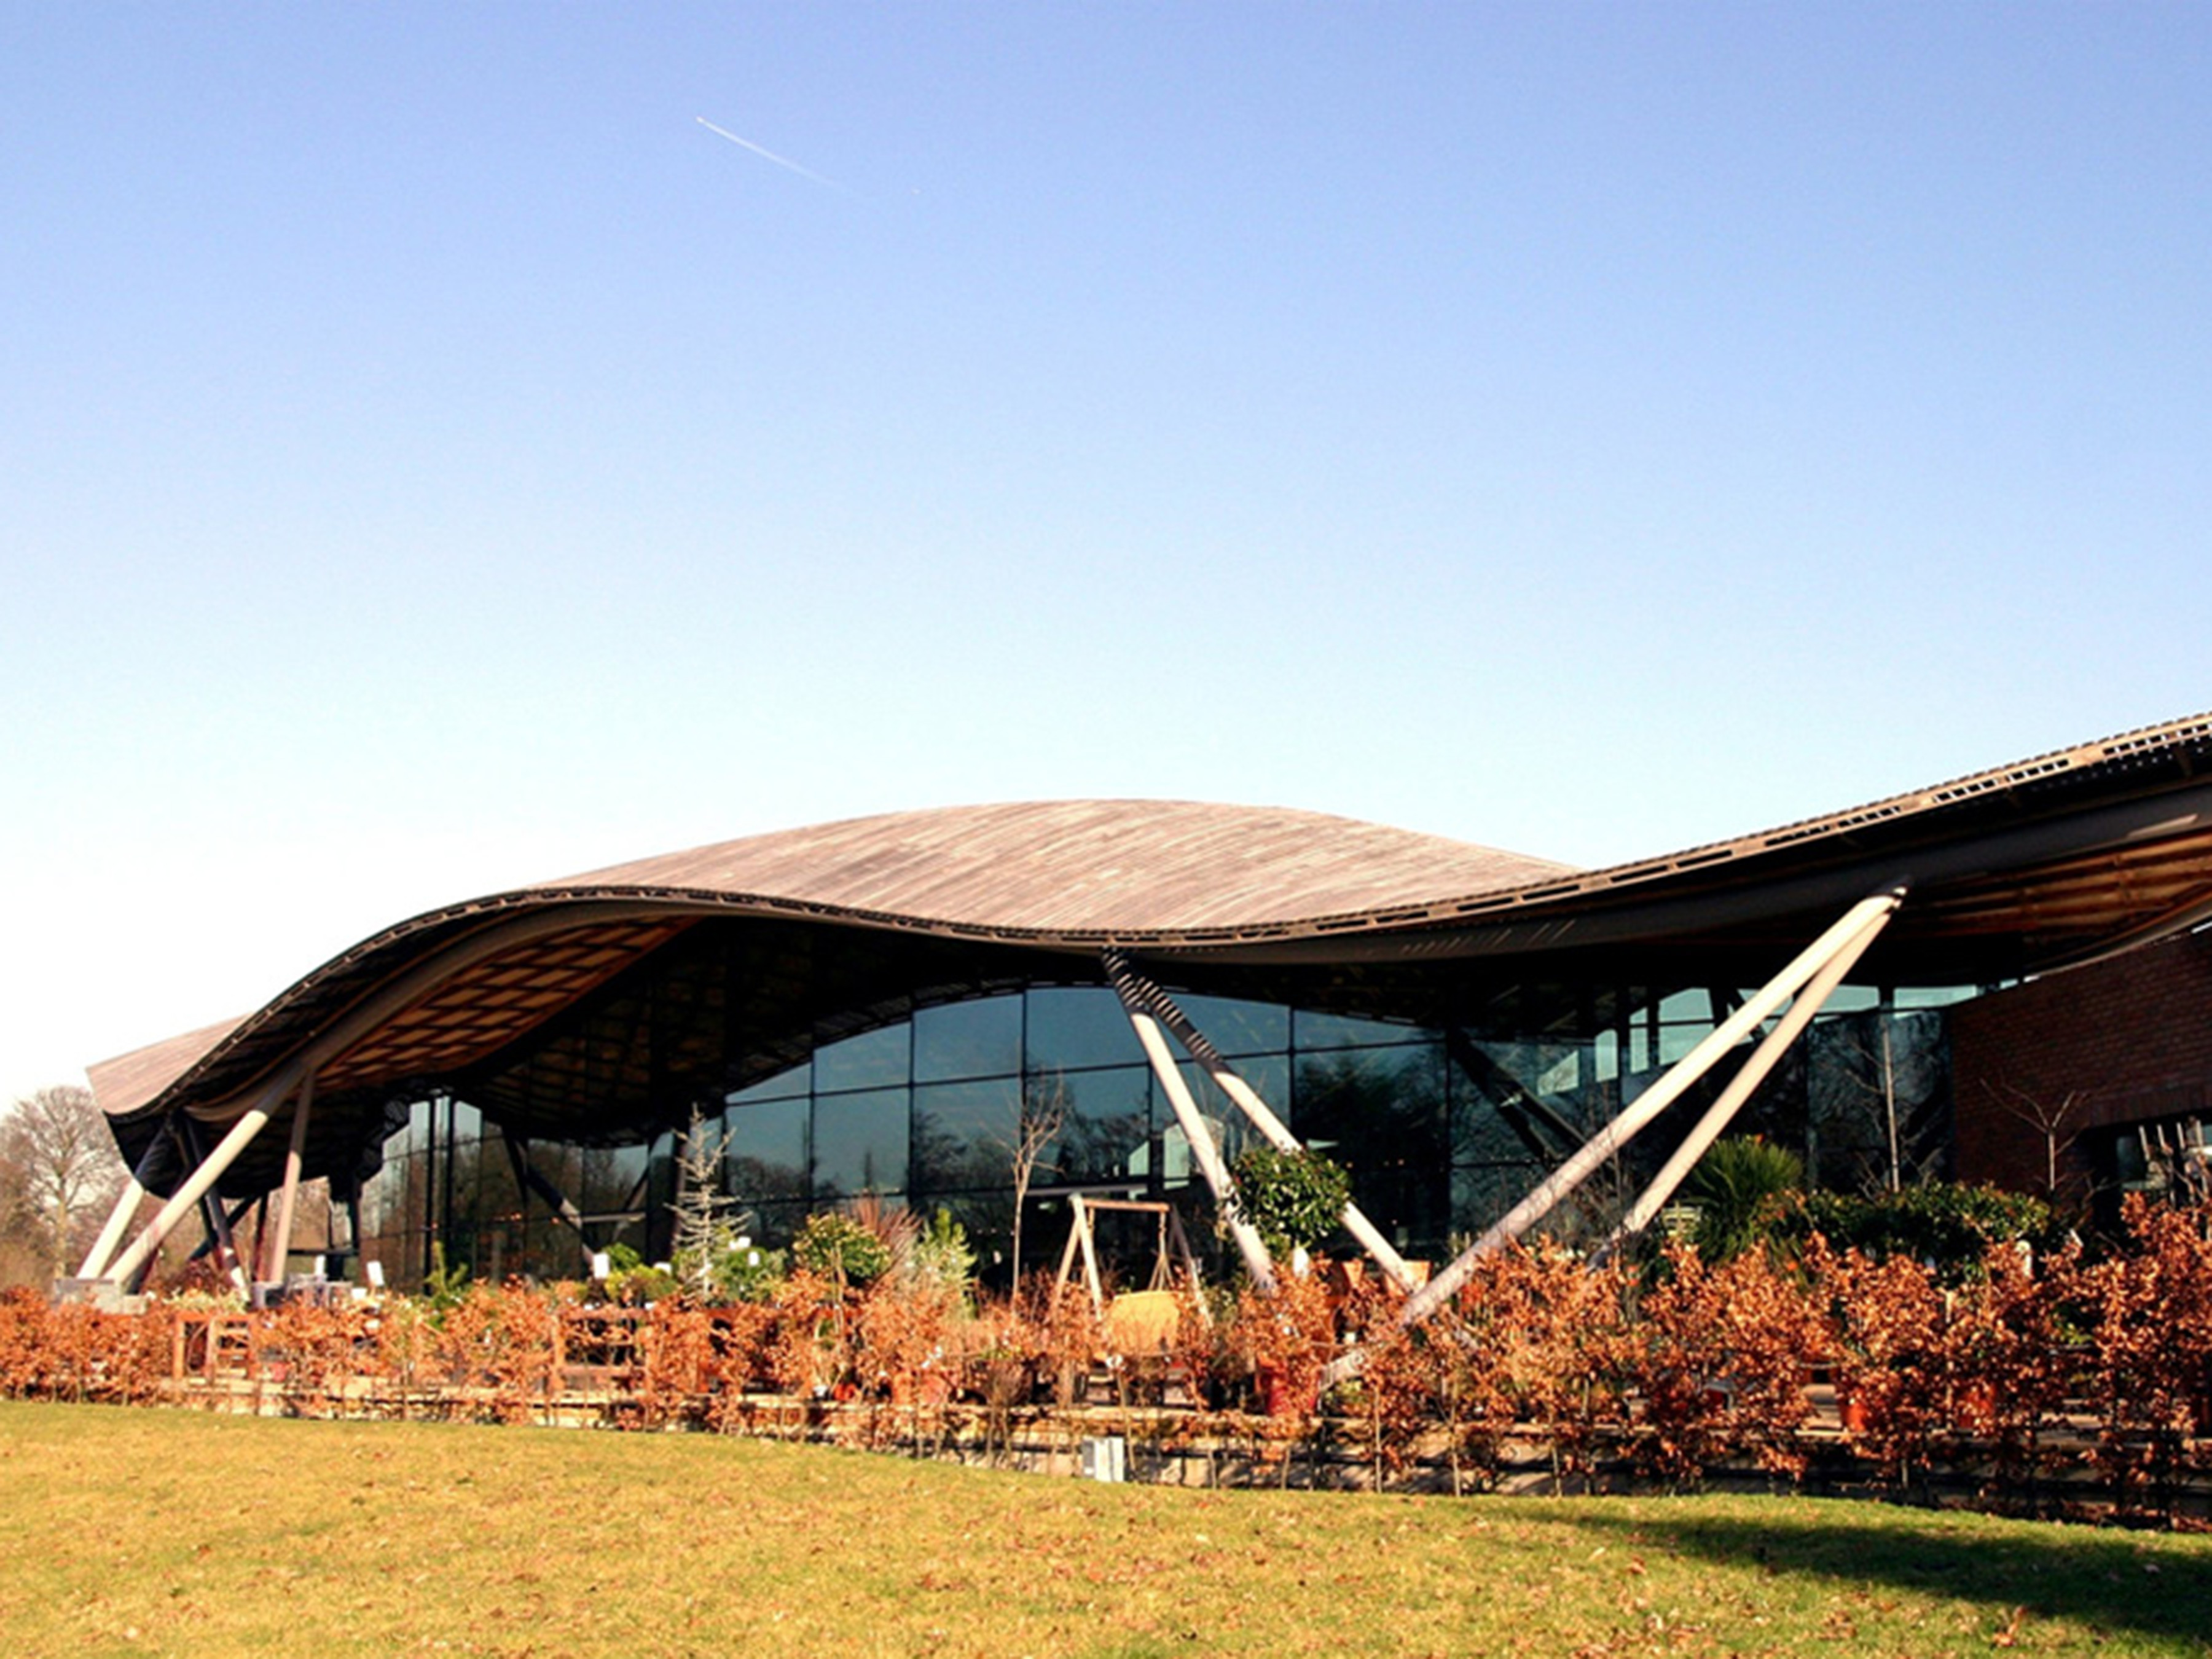
\includegraphics[width=2\paperwidth]{savill_a.jpg}};
\end{tikzpicture}
\clearpage
\begin{tikzpicture}[remember picture,overlay, inner sep=0pt]
	\node[anchor=north west, xshift=-0.5\pgflinewidth-\paperwidth, yshift=0.5\pgflinewidth] at (current page.north west){
	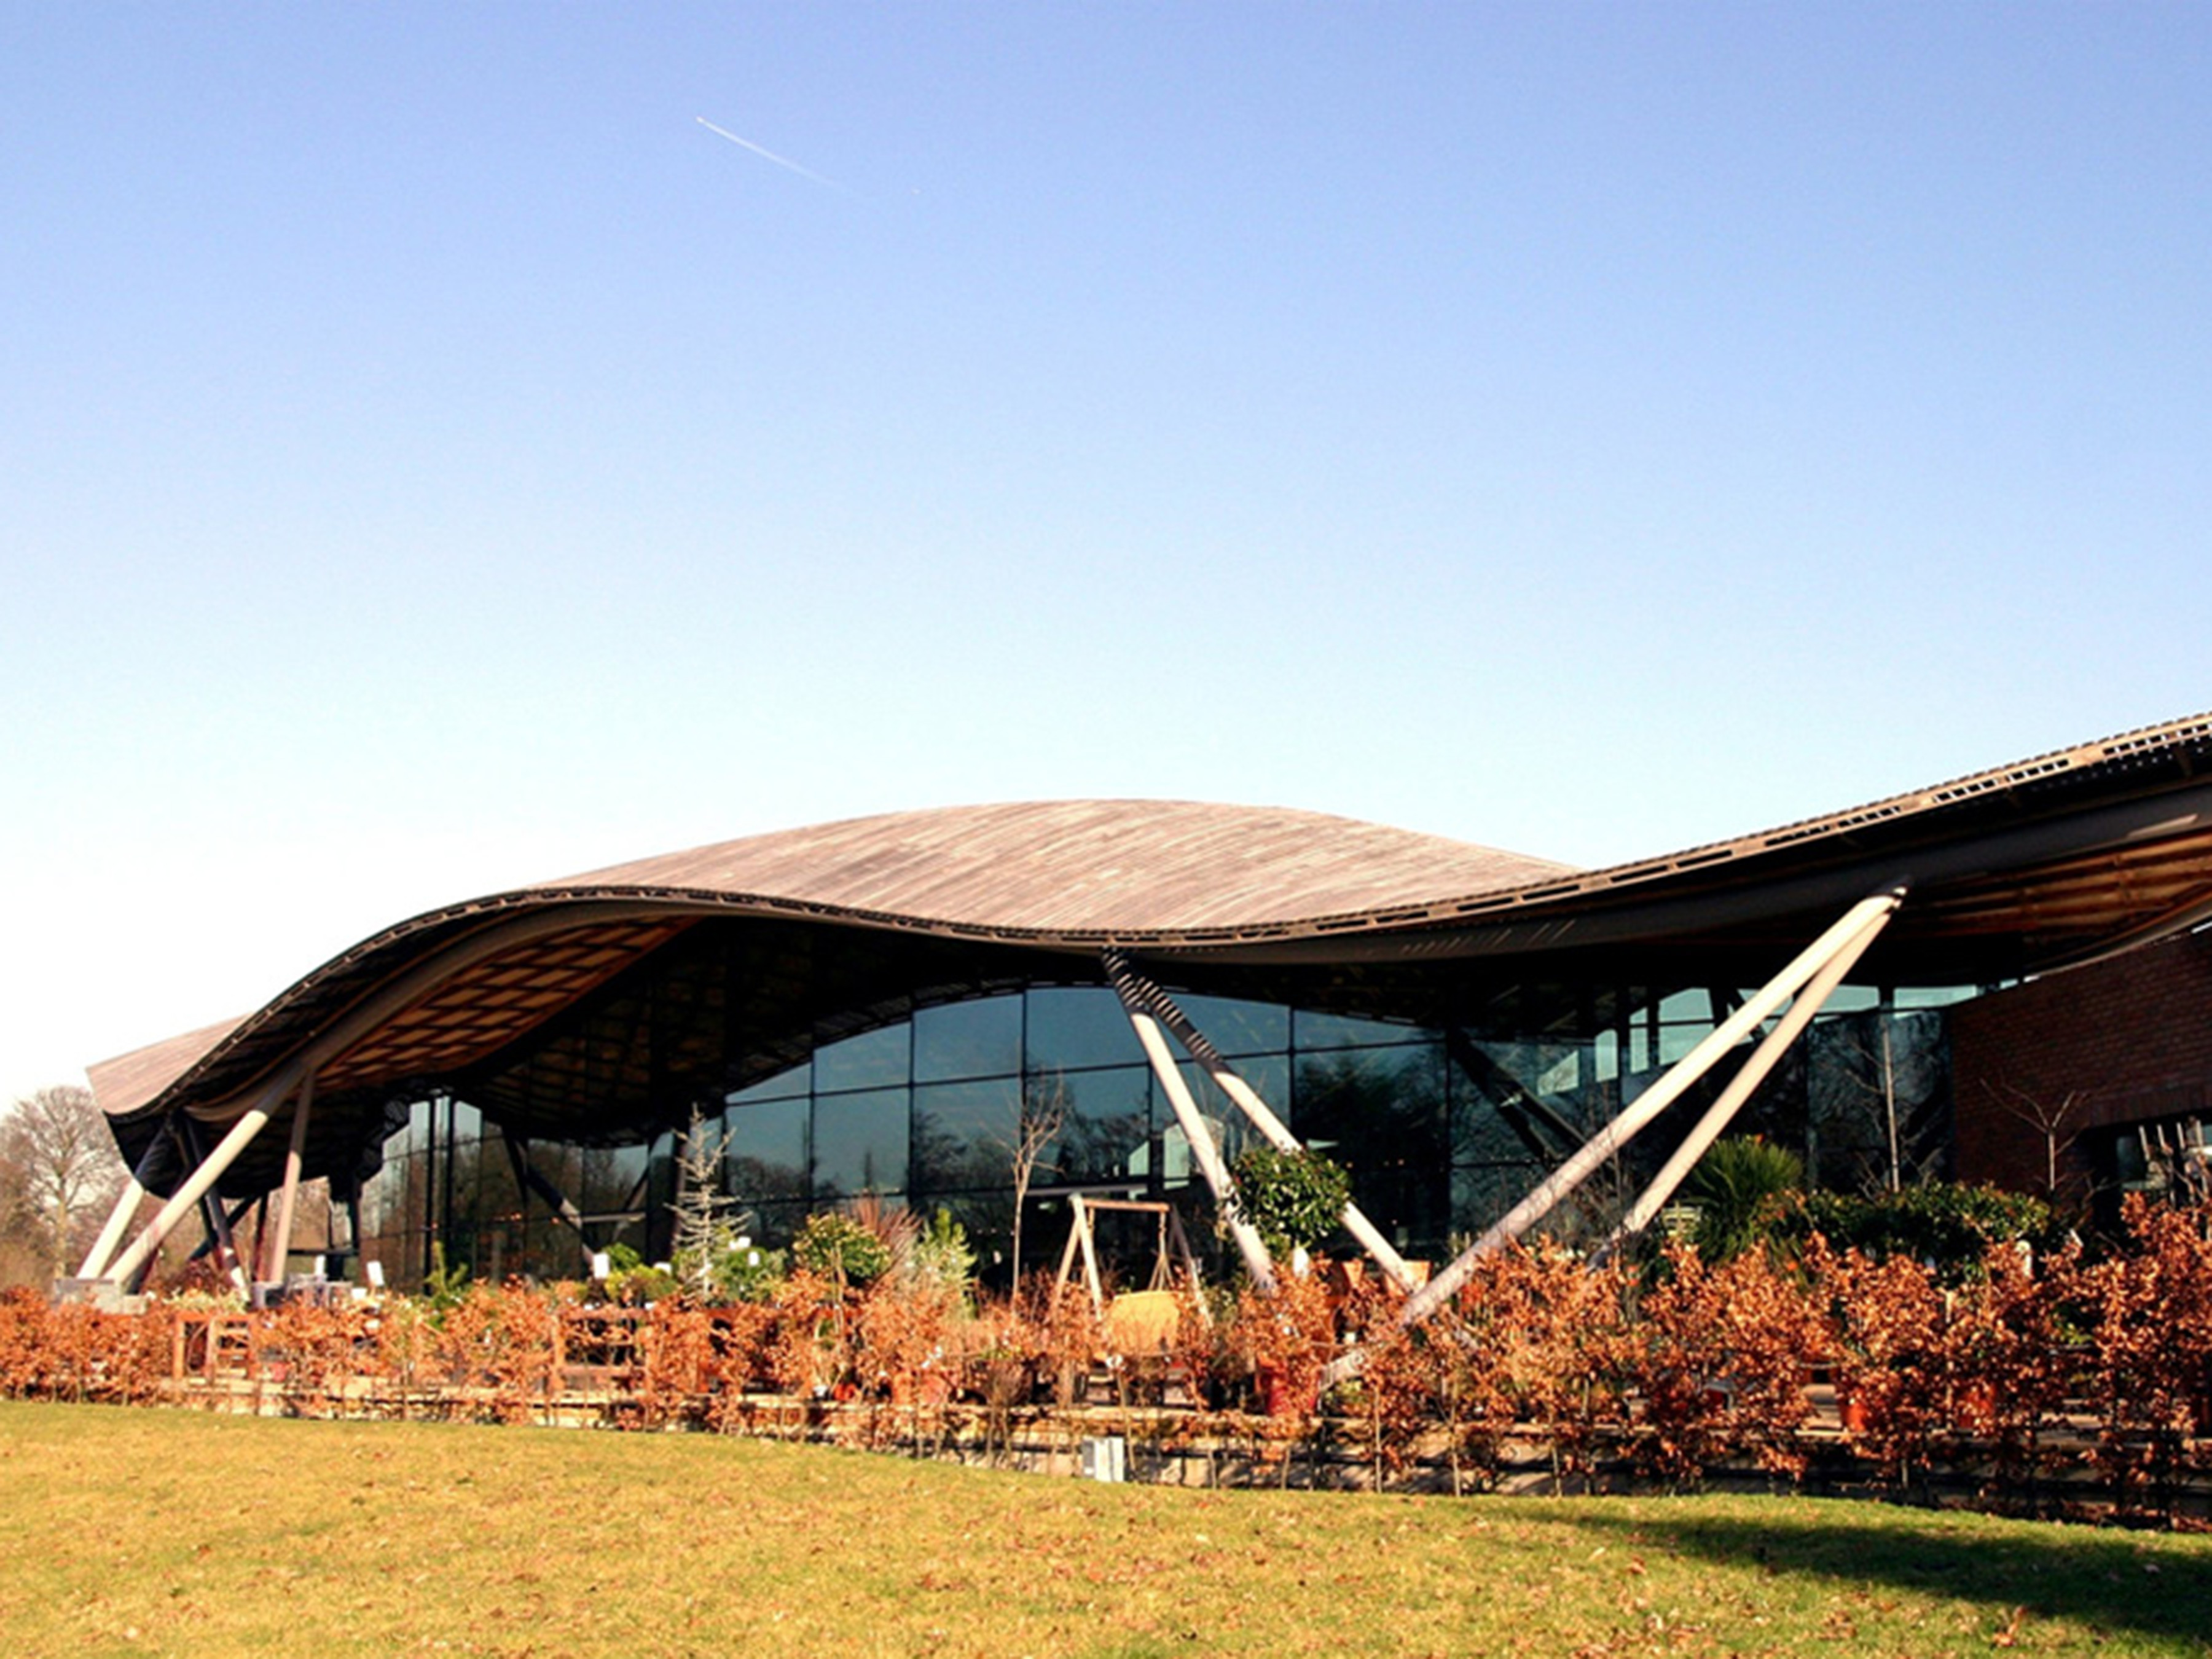
\includegraphics[width=2\paperwidth]{savill_a.jpg}};
\end{tikzpicture}


%%%%%%%%%%%%%
\clearpage
\kant[1-2]

\cleartoleftpage
\begin{textblock*}{10cm}[0,0](0cm,0cm)\noindent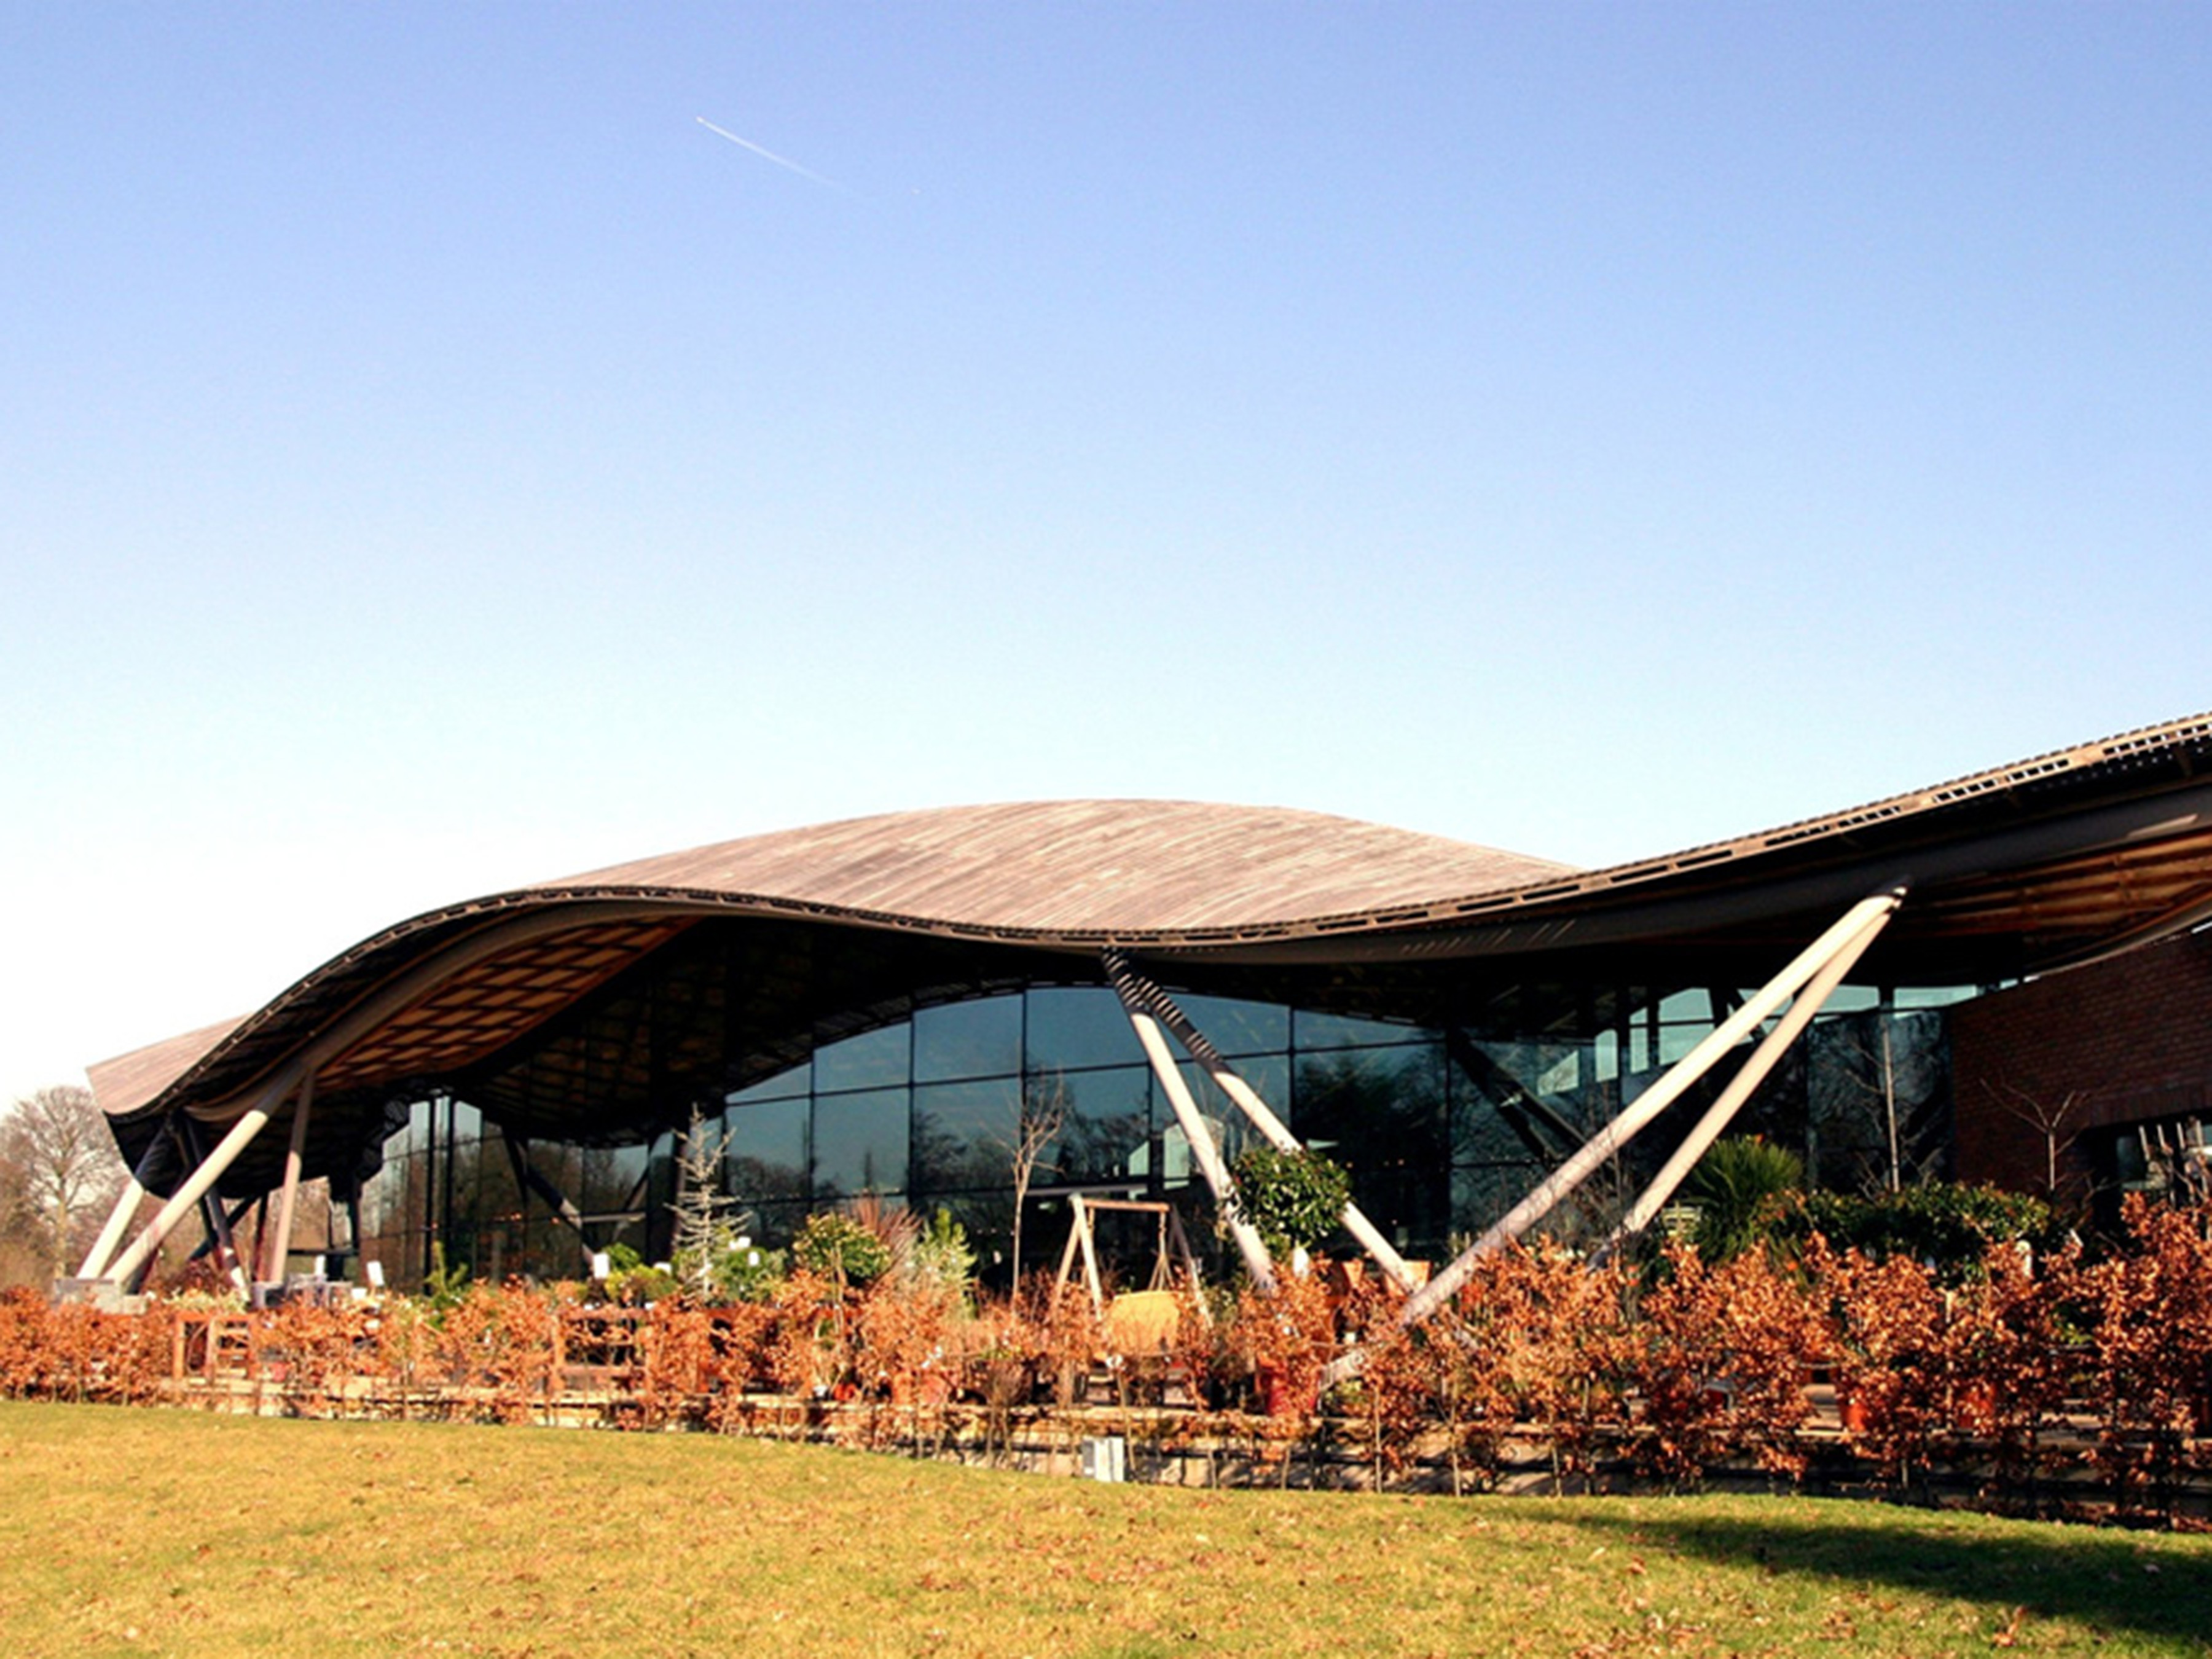
\includegraphics[width=10cm]{savill_a.jpg}\end{textblock*}


% \clearpage
% skdmlskdmslkd
% \begin{tikzpicture}[remember picture,overlay,inner sep=0pt]
% 	\node[anchor=north east,inner sep=0pt] at (current page.north east)
% 	{
% 	\begin{minipage}{\paperwidth}
% 		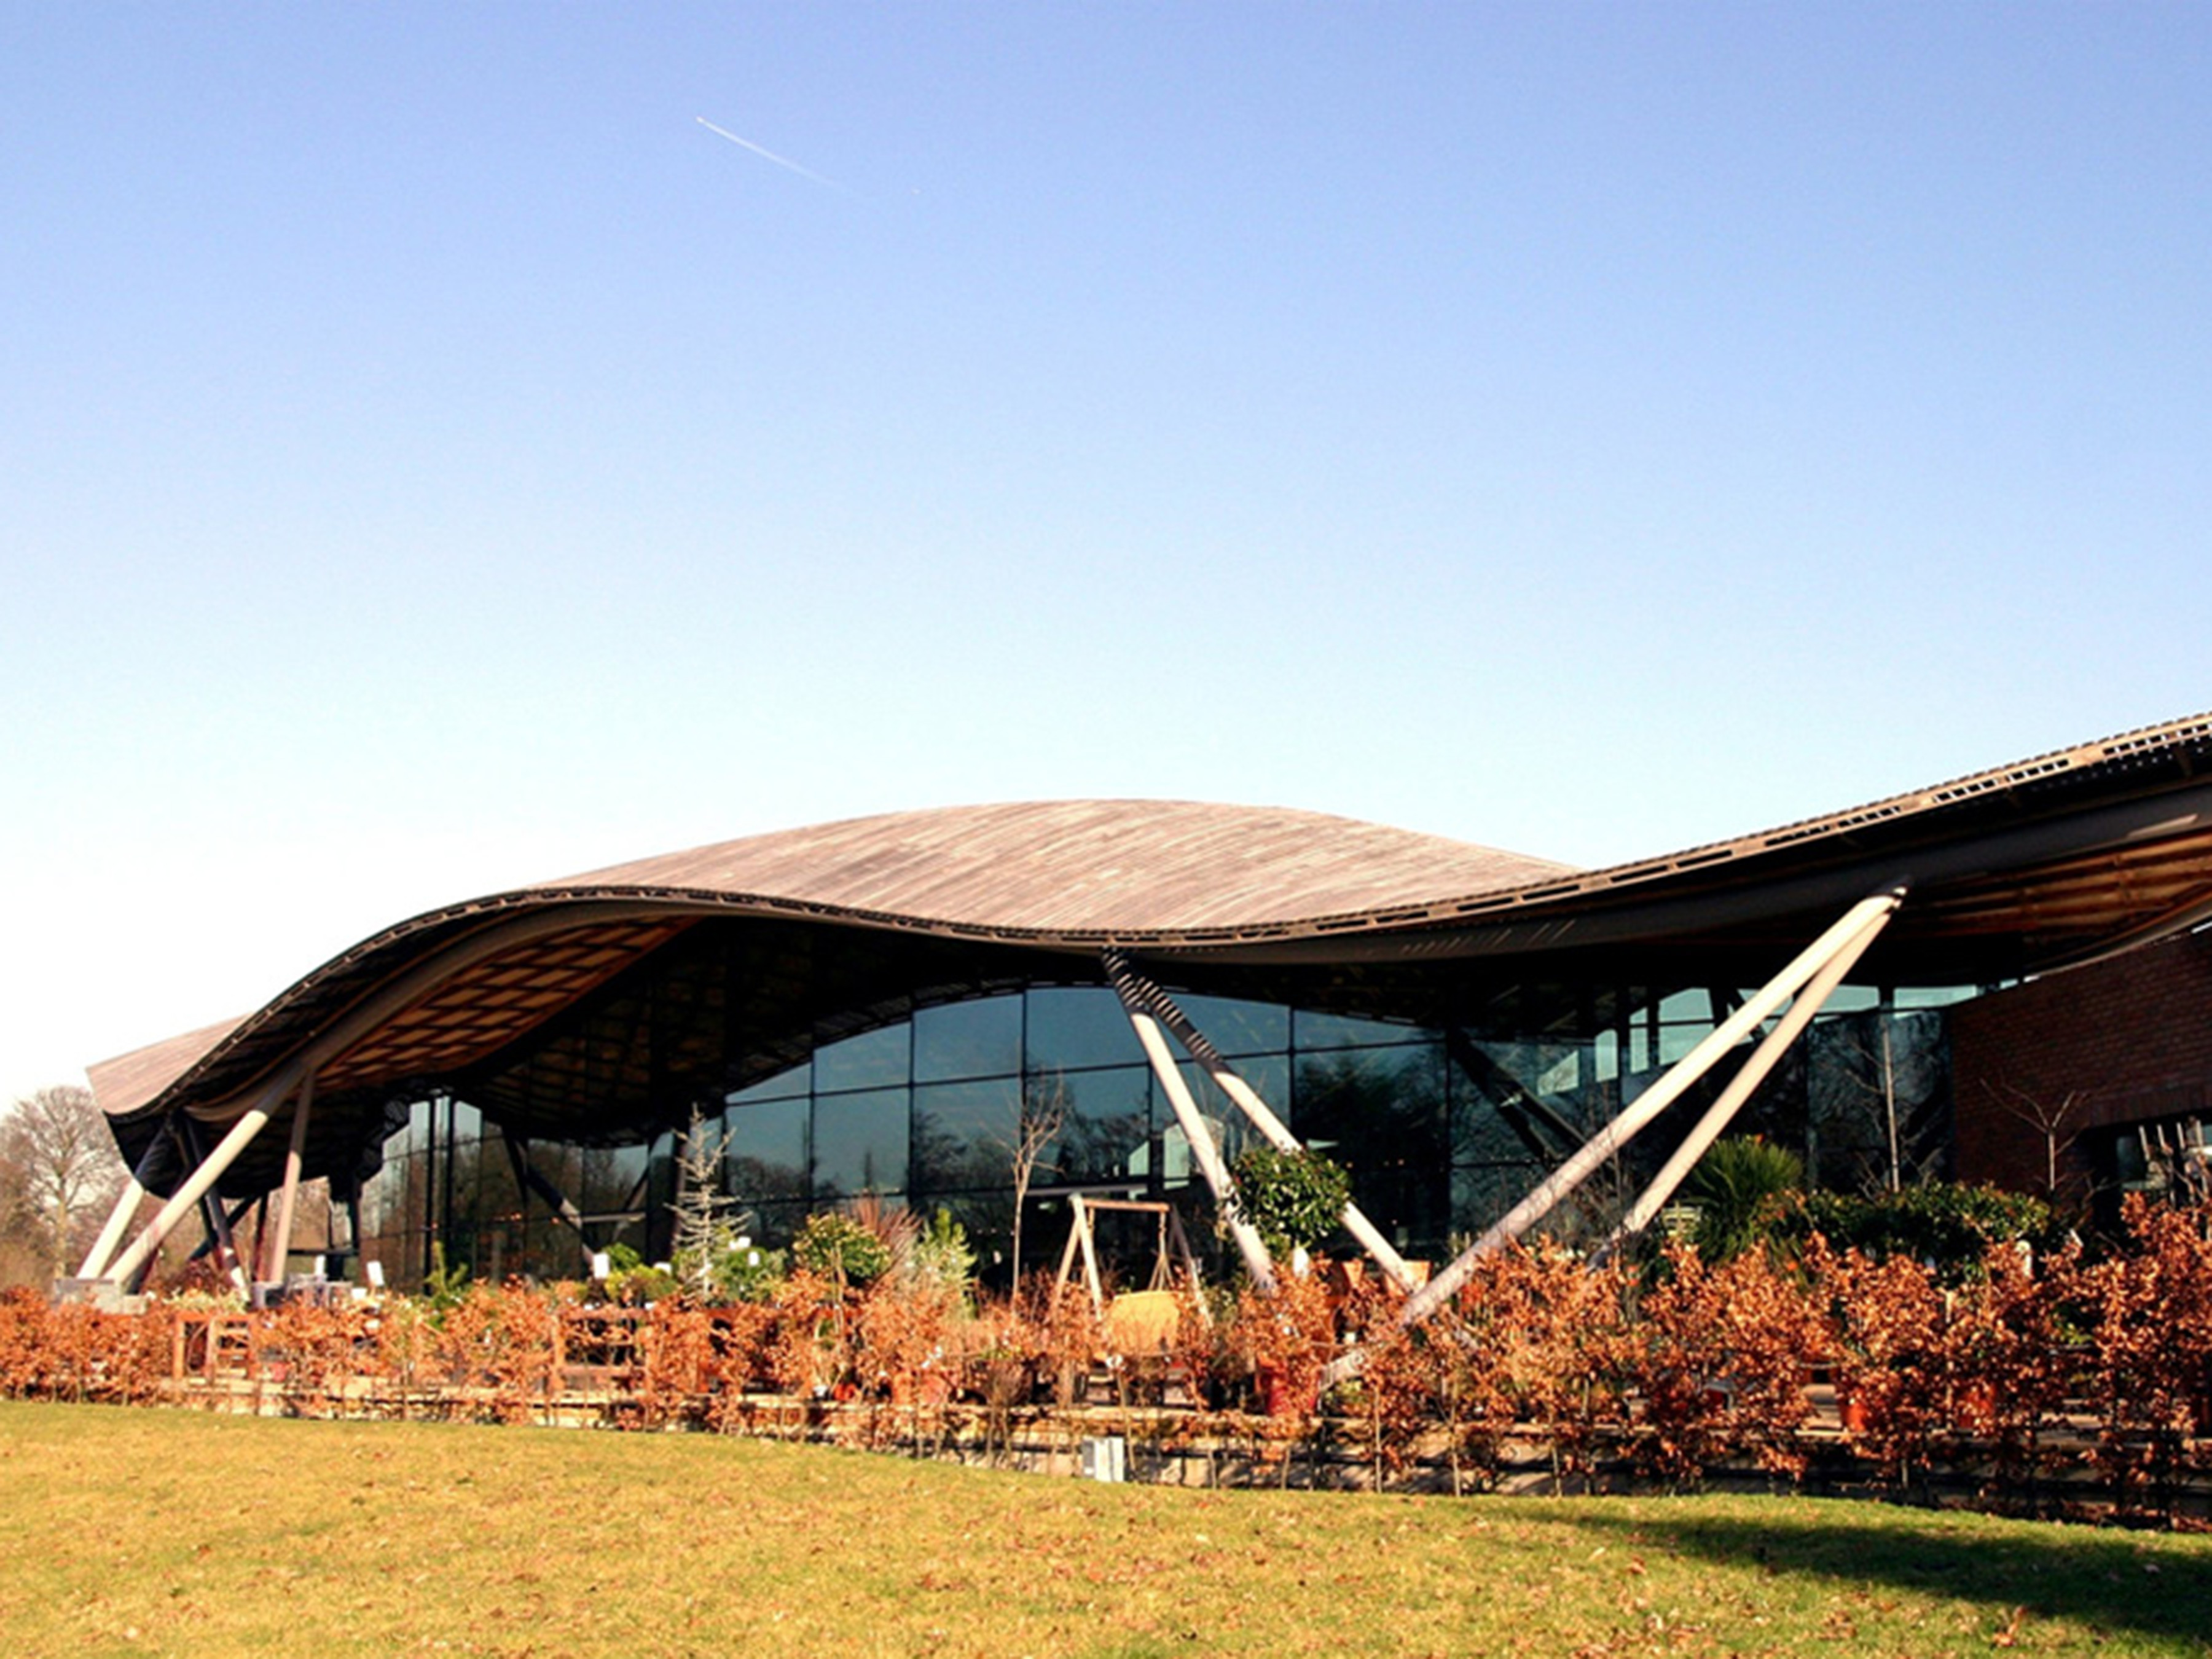
\includegraphics[width=\paperwidth]{savill_a.jpg}
% 		\captionof{figure}{sdsdksdmskdms}
% 	\end{minipage}
% 	};
% \end{tikzpicture}

% \clearpage
% \begin{tikzpicture}[remember picture,overlay]
% 	\node[anchor=north west,inner sep=0pt] at (current page.north west)
% 	{
% 	\begin{minipage}{\textwidth}
% 		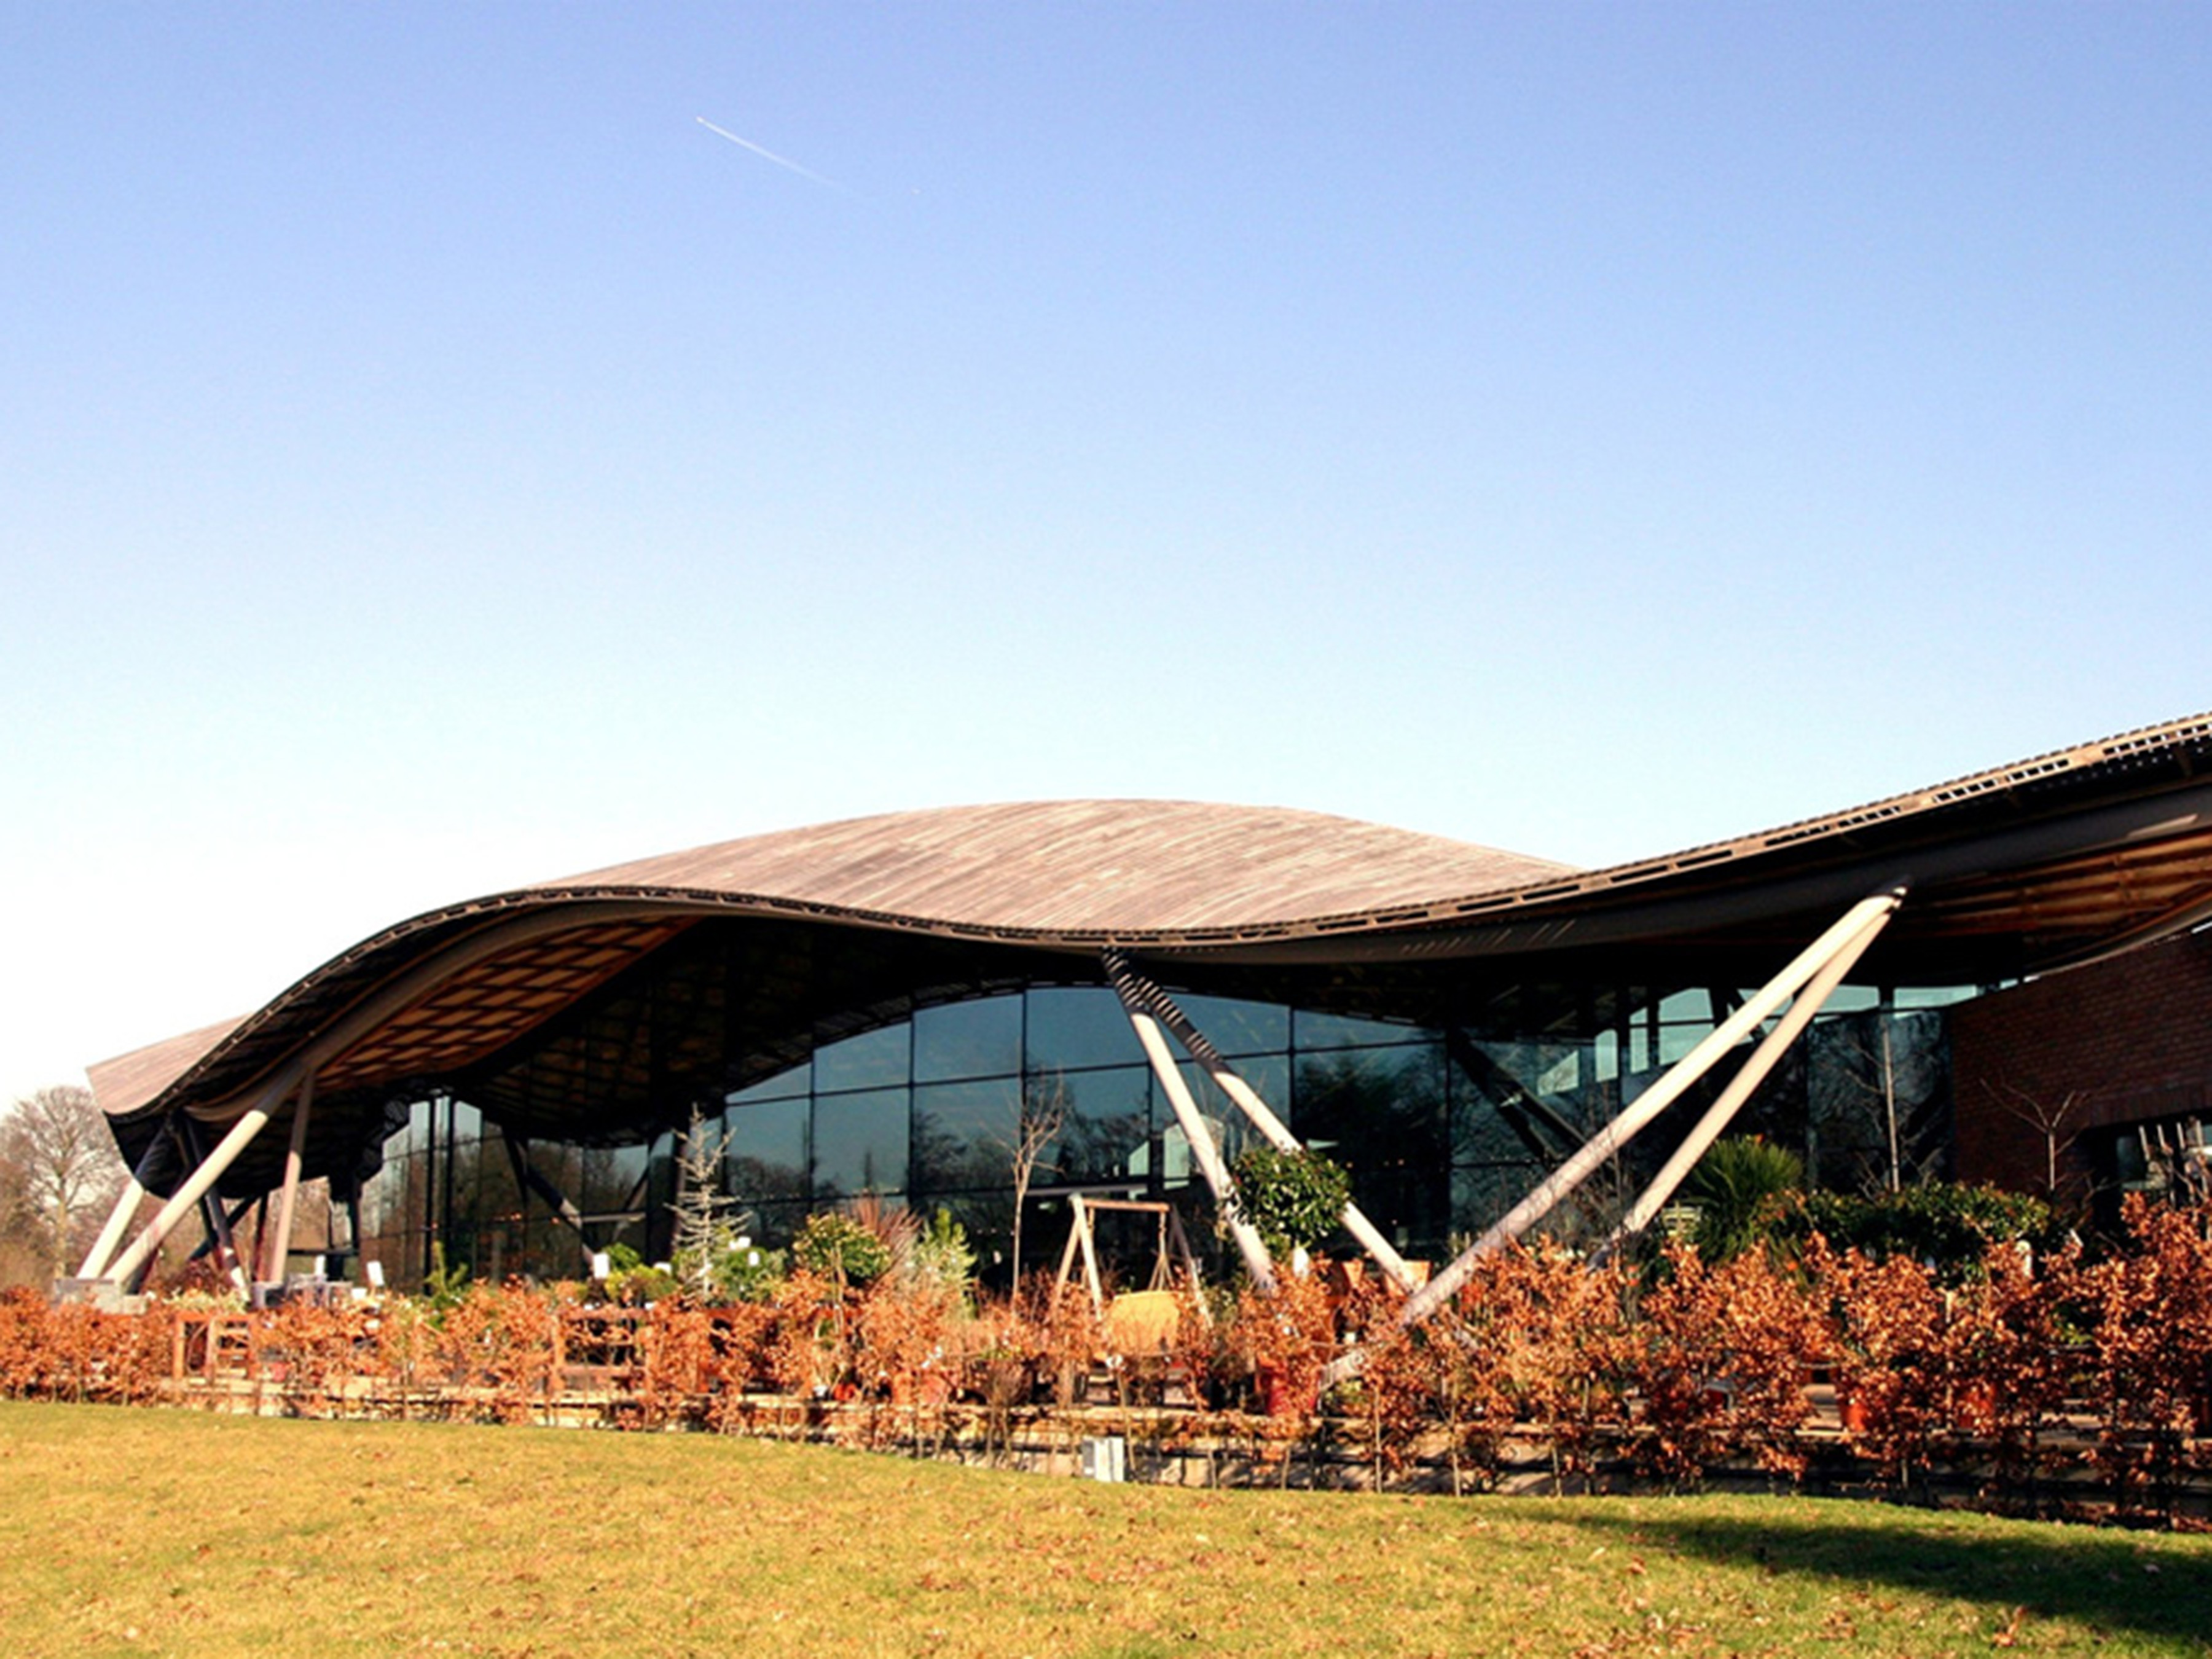
\includegraphics[width=\textwidth]{savill_a.jpg}
% 		\captionof{subfigure}{}{\label{fig:savill_d}}
% 	\end{minipage}
% 	};
% \end{tikzpicture}

% REF : \cref{fig:savill_d}


% \setlength{\unitlength}{1cm}
% % \begin{picture}(50,50)
% % 	\put(0,0){\hbox{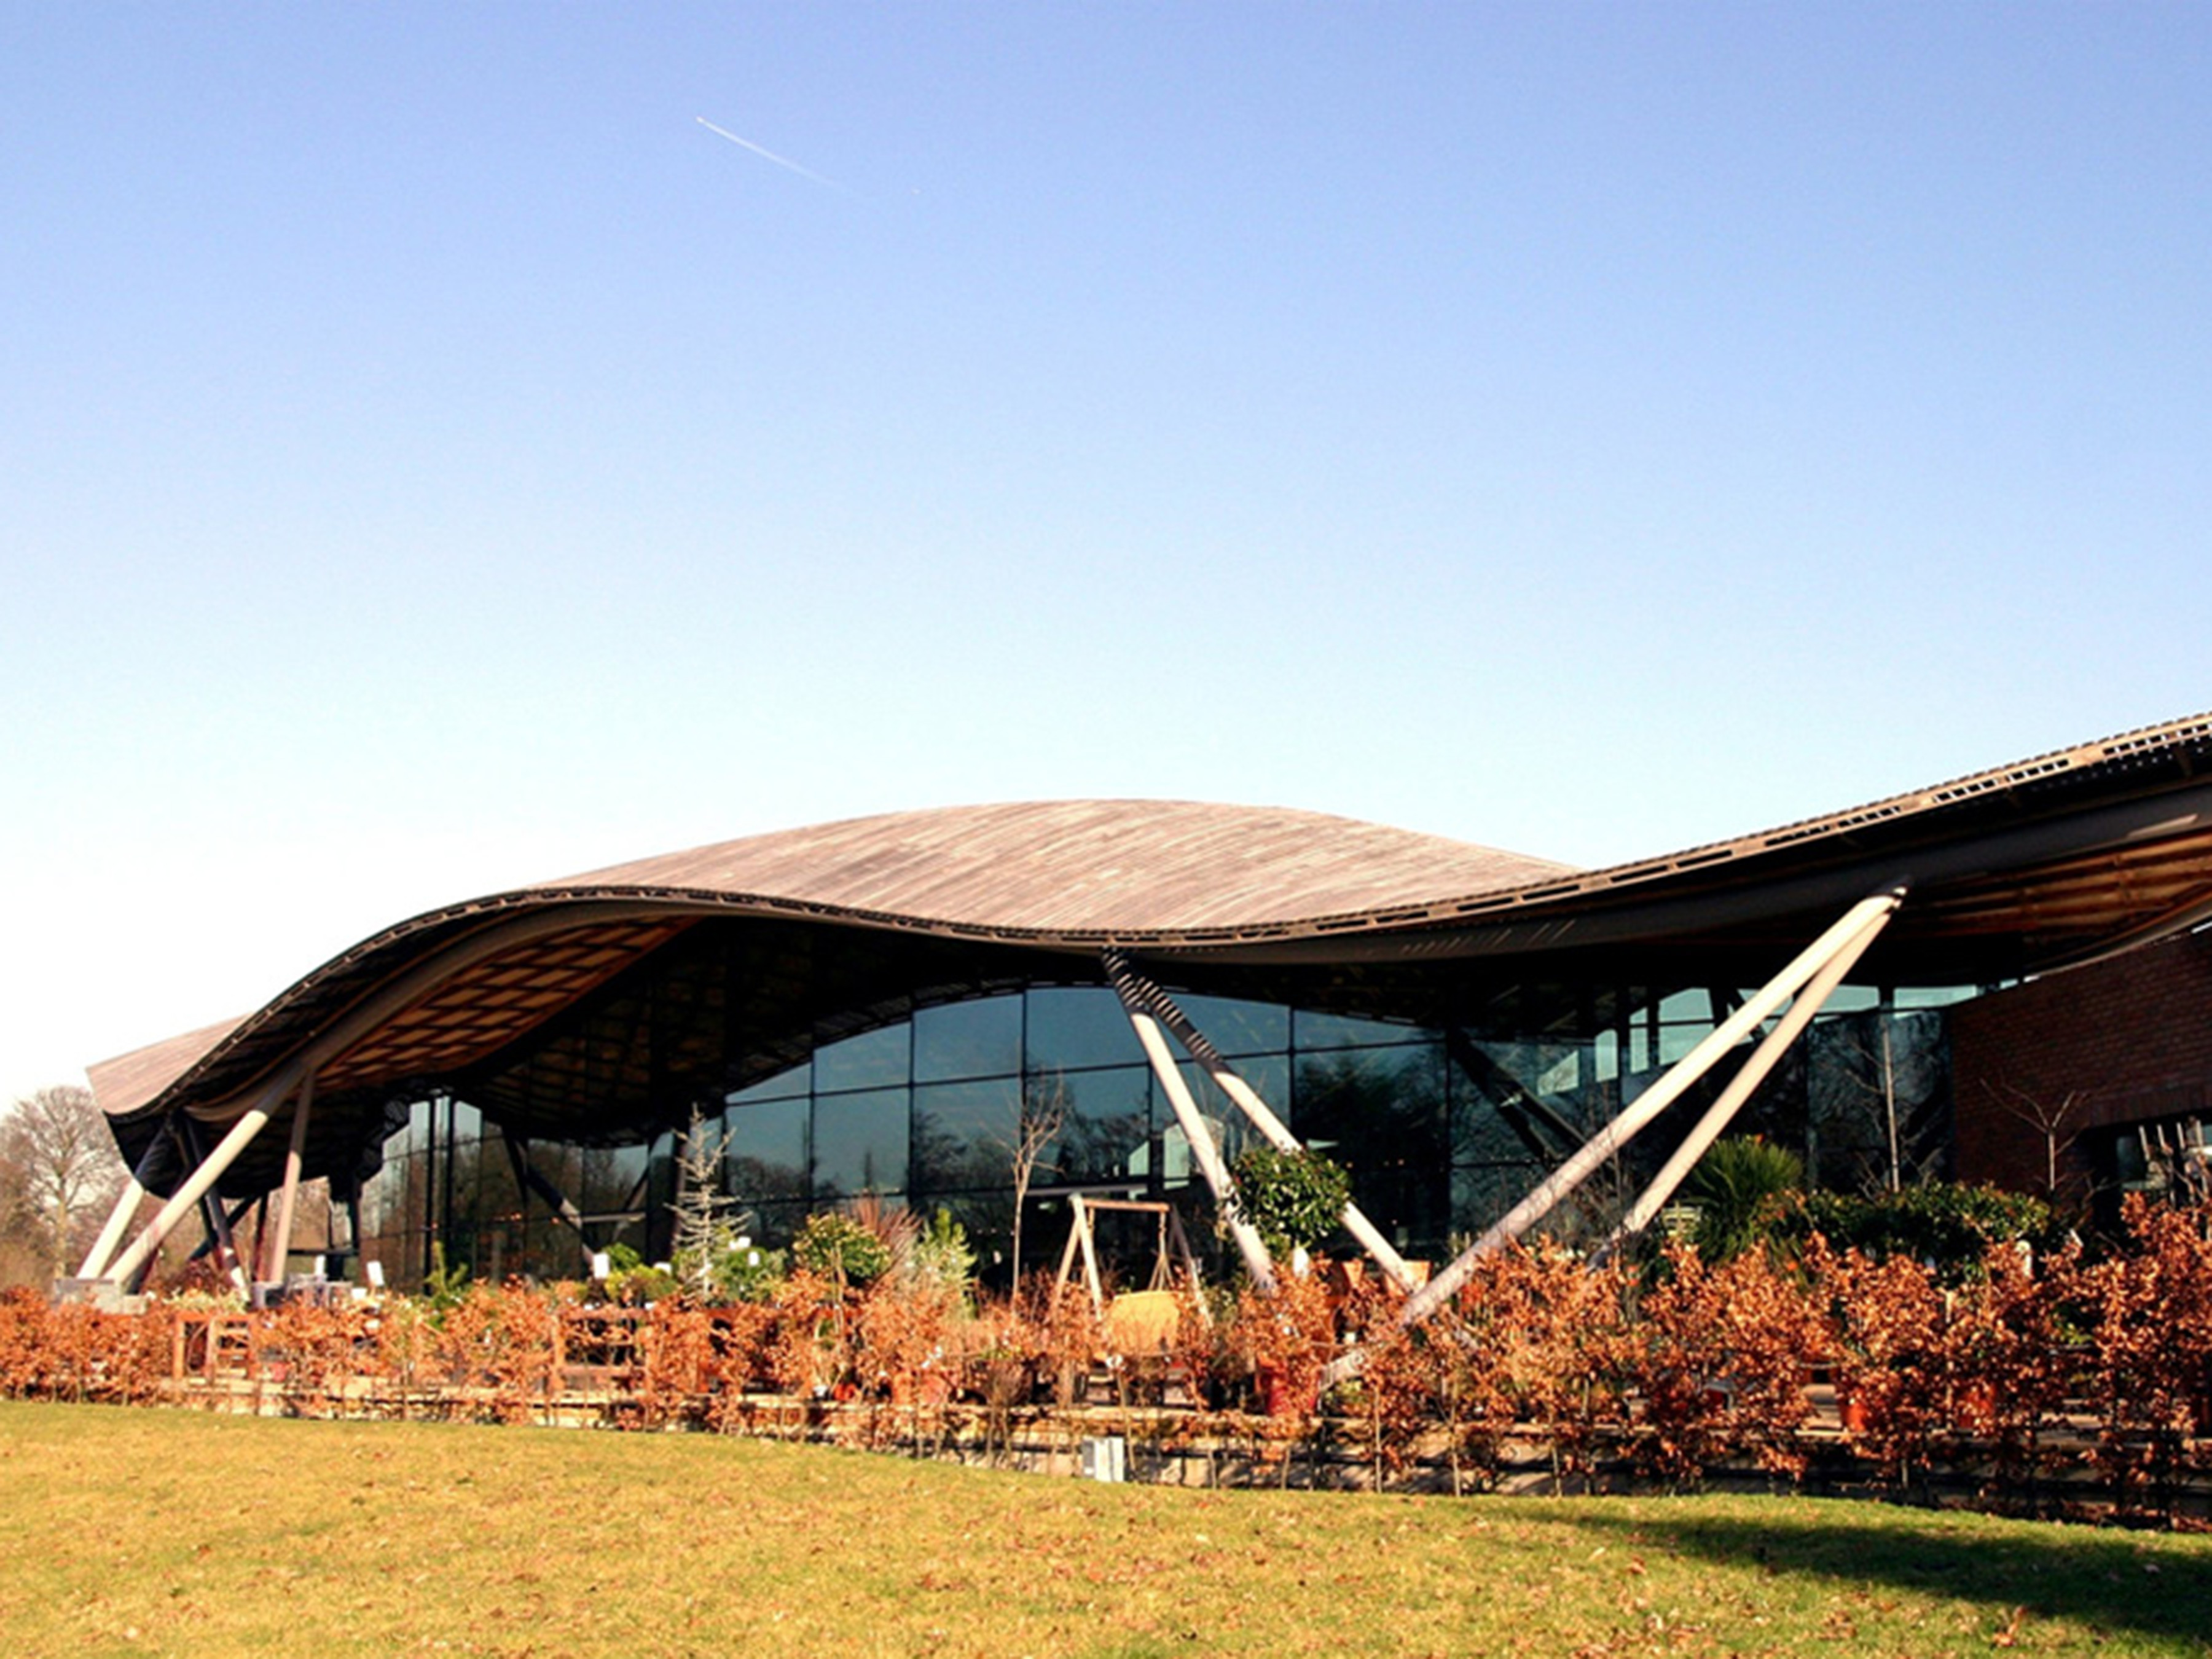
\includegraphics[width=\paperwidth]{savill_a.jpg}}}
% % \end{picture}

% \begin{picture}(0,-10)
% \put(0,0){%
% \begin{minipage}{0.48\linewidth}
% 	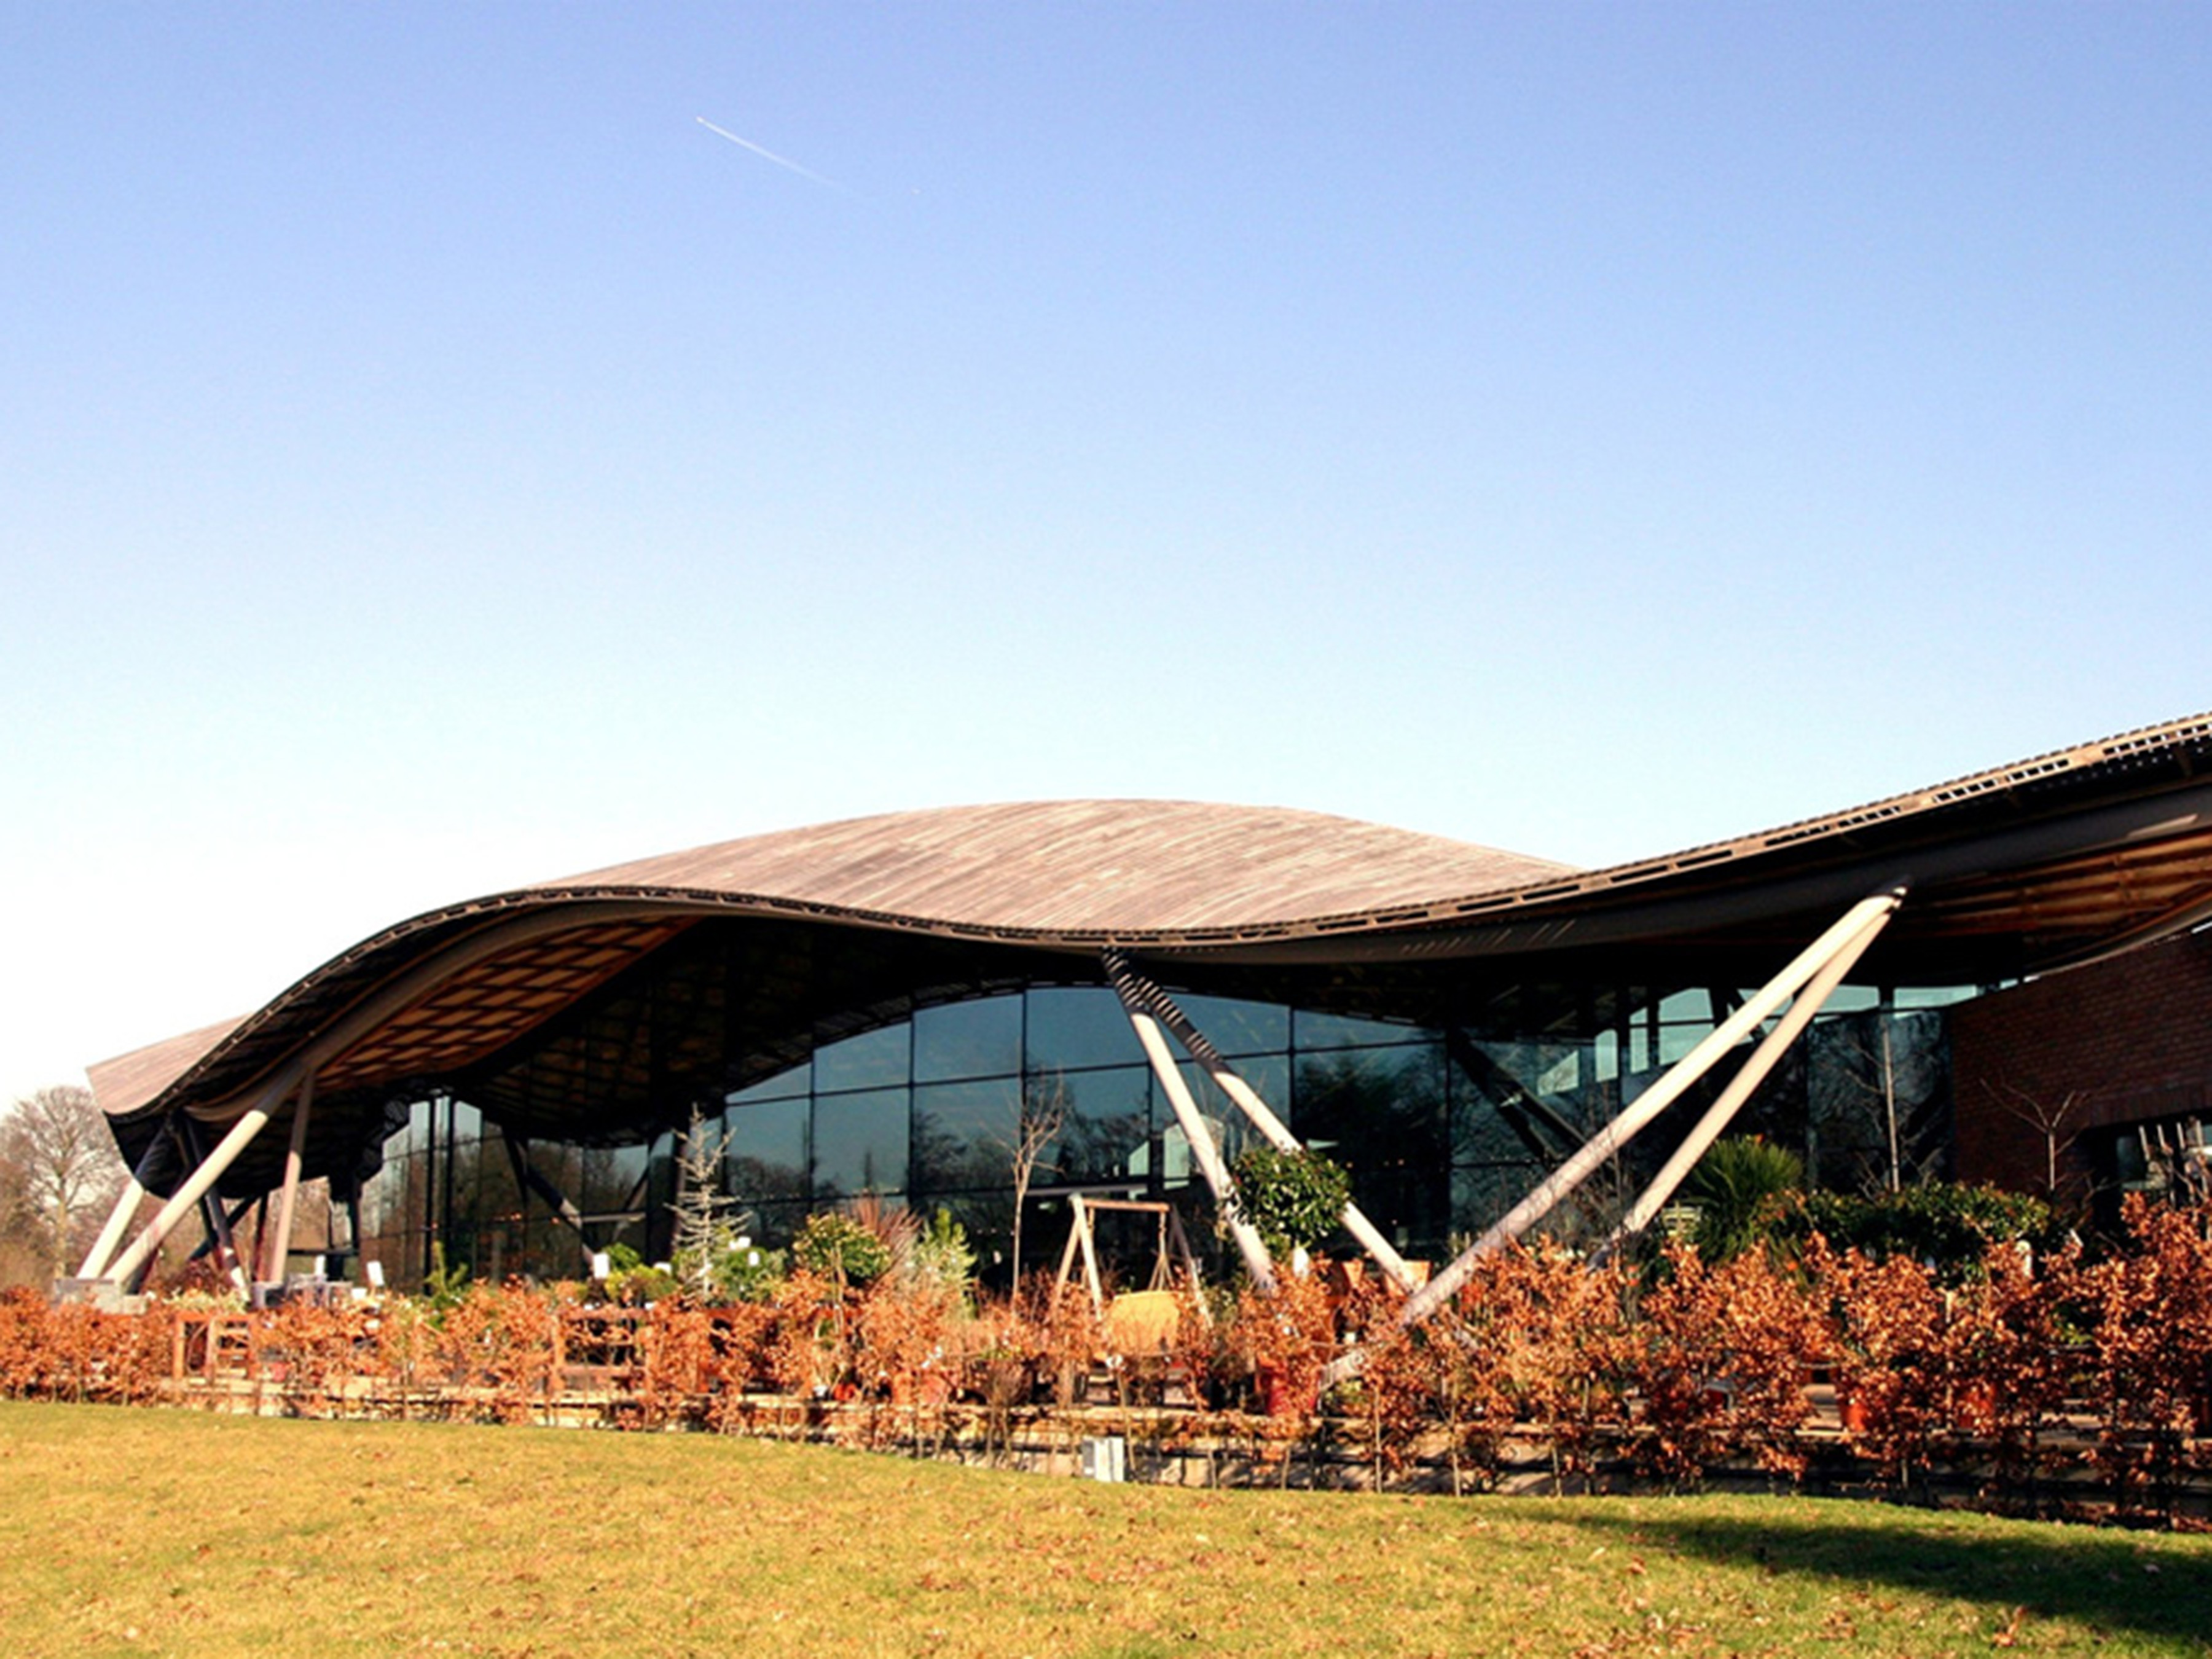
\includegraphics[width=\linewidth]{savill_a.jpg}
% 	\captionof{figure}{Some here}
% \end{minipage}%
% }
% \end{picture}

%  \begin{textblock}{2.5}(\GetX{2cm},\GetY{0cm})
% 	\raggedright
% 	Work is of two kinds: first, altering
% 	the position of matter at or near the
% 	earth’s surface relatively to other such
% 	matter; second, telling other people
% 	to do so.
% \end{textblock}

% \begin{textblock*}{10cm}[0,0](0cm,0cm)
% 	\raggedright
% 	Work is of two kinds: first, altering
% 	the position of matter at or near the
% 	earth’s surface relatively to other such
% 	matter; second, telling other people
% 	to do so.
% \end{textblock*}
\printbibliography[segment=\therefsegment,heading=subbibliography]
	% % % Author :  Lionel du Peloux
% Contact : lionel.dupeloux@gmail
% Year : 2017

\newrefsegment
\chapter{This is a very very very very very very long title}

\section{This is a very very very very very very long section}
%===================

This chapter is meant to define and introduce what elastic gridshell structures are. It develops a comprehensive but precise view of the numerous knowledge and know-how that gravitate around this concept.

\subsection{Overview}
We naturally begin this chapter by defining the notion of elastic gridshell and the context in which this technology arose (see \cref{sec=gsdef}). We briefly highlight the benefits of composite materials for this kind of structure. We then propose two thorough reviews~: the first one is dedicated to known built elastic gridshell structures (see \cref{sec=review_project}) while the second one is a literature review of the main works related  to the topic of elastic gridshells (see \cref{sec=review_research}).

\subsection{Contributions}
%Here, we summarize our contributions that are presented in this chapter~:
\begin{itemize}
\item We establish a chronological review of known built elastic gridshells, from the very beginning of this technology to the present time. We reveal the richness of this concept by exhibiting the great variety of realised projects. We discuss the specificities brought by each one of these projects.
\item We establish an up-to-date review of the existing scientific literature, crossing multiple fields of research (geometry, mechanics, material, \telp{}).
\end{itemize}

\section{Definition}\label{sec=gsdef}

The invention of the \emph{elastic gridshell} concept is commonly attributed to Frei Otto, a German architect who devoted several years to gridshells. In 1975 he achieved the famous \emph{Mannheim Multihalle} \cite{Happold1975}, a wooden shell of 7500~m\textsuperscript{2}, in collaboration with the engineer Edmund Happold (Arup).
Literally, the word \textquote{gridshell} refers to grids behaving like shells~: from a mechanical point of view that means stresses acting on the structure are mainly transmitted through compression and tension. These structures can cross large-span with very little material.

However, according to the historic evolution of the concept, to characterise a gridshell as the combination of a structural concept (a grid behaving like a shell, see \cref{sec=def_topo}) and a specific construction process (see \cref{sec=def_erec}) using the bending flexibility of the material (see \cref{sec=def_flexibility}) seems to be more accurate. The project of Mannheim -- in which a wooden regular and planar grid, lacking shear stiffness, is elastically deformed up to a targeted shape with the help of stays, and then braced and covered -- is regarded as the starting point of this new concept (see \cref{fig:multihalle}).

The project of Mannheim is regarded as the starting point of this new concept for which a wooden regular and planar grid, lacking shear stiffness, is elastically deformed up to a targeted shape with the help of stays, and then braced and covered. This type of gridshell, known as elastic gridshell, offers a very elegant manner to materialise freeform shapes from an initially flat and regular grid, which obviously has many practical benefits~: planar initial geometry, standard connection nodes, standard profiles and so on.

Note that the term \emph{rigid gridshell} is often opposed to the term \emph{elastic gridshell} to indicate reticulated structures that behave like shells but are not formed in an active-bending process.

\subsection{Structural typology}\label{sec=def_topo}
% ------------------------------------------
Their mechanical behaviour is very similar to the one of real shells even if the material is discrete and located in a grid more or less open. Moreover, gridshells benefit from the same advantages as the ones showed by an eggshell : they can cross large span using a low amount of material. Their stiffness is mainly linked to their double-curved shape.


\subsection{Material flexibility for structural rigidity}\label{sec=def_flexibility}
% ------------------------------------------
In this field of application, composite materials like glass fibre reinforced polymer (GFRP) could favourably replace wood, where both resistance and bending ability of the material is sought \cite{Douthe2010a}. The stiffness of the structure does not derive from the intrinsic material rigidity but principally from its geometric curvature. Ideally, the composite profiles are produced by pultrusion, an economic continuous moulded process. The standardisation of the process guaranties very stable material and mechanical properties. It frees designers from the painful problematic of wood joining and wood durability. The characterisation of this material is presented further in the thesis (see \cref{sec=design_gfrp}).
Because the in-plane stiffness of the grid also plays a major role in the resistance to buckling, this question was considered with care. The bracing of the grid was first achieved by preventing the nodes to turn once the grid was erected. This was done by creating some friction in the nodes when tightening the bolts linking the laths, after the grid was erected. Then, additional bracing cables were put in the grid.

Finally, the project of Mannheim was a key project in the development of modern lightweight structures. Great engineers were born in touch with Frei Otto, following his footsteps or collaborating with him. This heritage has irrigated for several decades the engineering of lightweight structures in Europe and gave birth, directly or indirectly, to several studios among which we can cite \emph{Buro Happold} and \emph{Schlaich Bergermann \& Partner}.

\subsection{The dry period : 25 years from Mannheim to Hannover}

Although the experience of Mannheim proved the feasibility and the potential of gridshell structures for large-scale projects, it also revealed that these projects were subject to an incredible complexity in terms of structural design, geometry, modelling, testing, team work, construction methods \telp{} At that time, very few people could pretend to master all the knowledge and techniques required to design and built timber gridshells and developed in the bosom of the \emph{Institute for Lightweight Structures} in Stuttgart.

This project was obviously well ahead of its time and the engineering cost to design such structures was probably prohibitive considering the tools available at that time. This certainly explains why no elastic gridshells were built during the 25 following years, despite the optimism of the pioneers of the Multihalle.\footnote{\blockcquote[]{Harris2003}{For many years after its completion, Happold promoted the benefit of the timber gridshell as a construction technique and stated that he could not understand why it had not been adopted more widely. He perceived the benefits to be in the efficiency of the construction method to enable doubly curved (shell) structures to be constructed quickly and cost effectively.}.}

Note that around 1975 small workshop and experiments lead to the construction of several but small elastic gridshells, as reported in \cite{IL10}. A non-exhaustive but quite extensive list of known executed gridshell projects is presented in \cref{fig:projectsbymaterial}. The dry period is clearly visible.

\subsection{The signs of a renewal : Dorset and Doncaster}\label{sec=signs}

It is only 20 years later that gridshells started to reappear, in the late 90's mainly in the United Kindom, and for projects that had interest in environmental problematics.

\subsubsection{Westminster Lodge, Dorset, England, 1995}
In 1995, a small student residence named \emph{Westminster Lodge} was built in Dorset, England. This dwelling was part of a larger project -- Hooke Park -- aiming at investigating how the local forest resources, in particular immature roundwood thinnings, could be better utilised. The project was lead by ABK, Frei Otto, Buro Happold and Cullinan Studio. Unlike Mannheim, the timber shell was bent and weaved rod by rod on a scaffold platform. But the structural system exhibited a double-layer gridshell pattern very similar to the one employed for the Multihalle (see \cref{fig:dorset_a}). The rods were made out of splice-jointed roundwood to form long-length poles of diameter \SI{200}{mm}. The development of this jointing technique, which could be produced directly in the forest, was part of the project's investigations \cite{Burton1998}. The grid was braced by a layer of diagonal boards nailed to the roundwood. The structure was finally cladded with a planted turf roof (see \cref{fig:dorset_b}).

\subsubsection{Earth Center, Doncaster, England, 1998}
At the same time, a project with a similar spirit arose for the \emph{Earth Center} in Doncaster, England.\footnote{\textquote{\href{http://grant-associates.uk.com/approach/earth-centre-forest-garden-grid-shells/}{The Earth Centre Forest Garden} was intended to demonstrate how managed woodland could supply the vast majority of all natural resources needed for human survival.}} The project planning started in 1994 and a series of small timber gridshells were designed by Buro Happold and then built in 1998. The landscape structures were single-layer timber gridshells made with oak laths. Once erected with a crane, the grids were braced with crossing diagonal stainless steel cables (see \cref{fig:doncaster_a}). Openings were possibly reinforced with curved timber frames (see \cref{fig:doncaster_b}).

These projects definitely trailed the technique in England and initiated the renewal period (see \cref{sec=renewal}). Although they remained small-scale projects for which modelling was achieved through physical models, they trained and restored partially the operational ability of Buro Happold to design timber gridshells as pointed by \citet{Harris2003}.



What was missing for elastic gridshells to re-emerge after the major experiment of Mannheim was probably the development of modern numeric tools to ease and speed up the design process.\footnote{\blockcquote[]{Harris2003}{The key to the modern use of timber gridshells is the development of computer methods in modelling complex three-dimensional shell structures. For the Mannheim structure, the primary method of form finding was the use of physical models. The Earth Centre structures were small and easily modelled using wire mesh, but when Buro Happold was commissioned to design the Japanese Pavilion for Expo 2000 in Hannover (Architect Shigeru Ban), it was apparent that much more sophisticated computer form finding and analysis would be necessary.}} Amongst those tools we should identify two main categories~: geometry processing softwares and structural analysis softwares. Recall that in the 70's, geometry processing was done through physical models and photographic measurements \cite[pp.~130-135]{IL10} while structural analysis was conducted through a compound of physical model testing with scaling techniques \cite[pp.~130-135]{IL13}, hand calculations and the very first numerical form-finding calculations \cite[pp.~184-193]{IL10} and finite element calculations \cite[pp.~210-217]{IL10}. In the late 90's, the rise in importance of computer methods offered new possibilities.

\subsubsection{Japan Pavilion, Hannover, Germany, 2000}
In 1997, architect Shigeru Ban began to collaborate with Frei Otto and Buro Happold to design the \emph{Japan Pavilion} for \emph{Expo 2000} in Hannover, Germany \cite{Ban2006}. This pavilion was a large-scale corrugated gridshell made out of cardboard tubes, about 75 meters long and 25 meters wide. Corrugations bring curvature, and therefore enhance the strength of the shell. The tubes were tied together with a fabric tape, a very low-tech joint (see \cref{fig:hannover_a}). The structure was covered with a paper membrane specially developed for the project to meet the requirements of the German fire regulations (see \cref{fig:hannover_b}). For the occasion, a new erection method was set up in which the grid was laid out not at the ground level but at a higher level on a hydraulic scaffold platform. From there, the grid was pushed up into position using the platform's jacks. It was found late that the cardboard tubes were subject to a high level of creep. This required the introduction of new timber arches to reinforce the gridshell and to enlarge the existing timber rafters intended to brace the grid and support the paper membrane (see \cref{fig:hannover_a}).

\subsubsection{Weald and Downland, Singelton, England, 2002}
The design of the \emph{Downland} gridshell began right after the completion of the Westminster Lodge (see \cref{sec=signs}) where architects from E. Cullinan Studio became acquainted with the engineers from Buro Happold. At Downland, the project team truly revived the technique of large-scale timber gridshells while bringing lots of improvements to the system. The building opened to the public in 2002. Its corrugated shape recalls the one of the Japan Pavilion from which it was inspired (see \cref{fig:downland_b}).

The building is 50 meters long and 12.5 to 16 meters wide, covering an area of about \SI{675}{m^2} for a height varying from 7 to 9.5 meters \cite{Harris2002}. The structure is a double-layer gridshell made of rectangular oak laths of cross-section \SI{50}{mm} x \SI{35}{mm} (see \cref{fig:downland_a}). To produce high grade timber elements, the continuous laths were re-formed from small carefully selected wood pieces, finger-jointed every \SI{60}{cm} in \SI{6.0}{m} length pieces. These pieces of lath were then scarf-jointed on site every \SI{6}{m} to obtained the desired length, up to \SI{50}{m}.
%\begin{figure}[t]
%		\hrule
%		\subfloat[][Interior view]{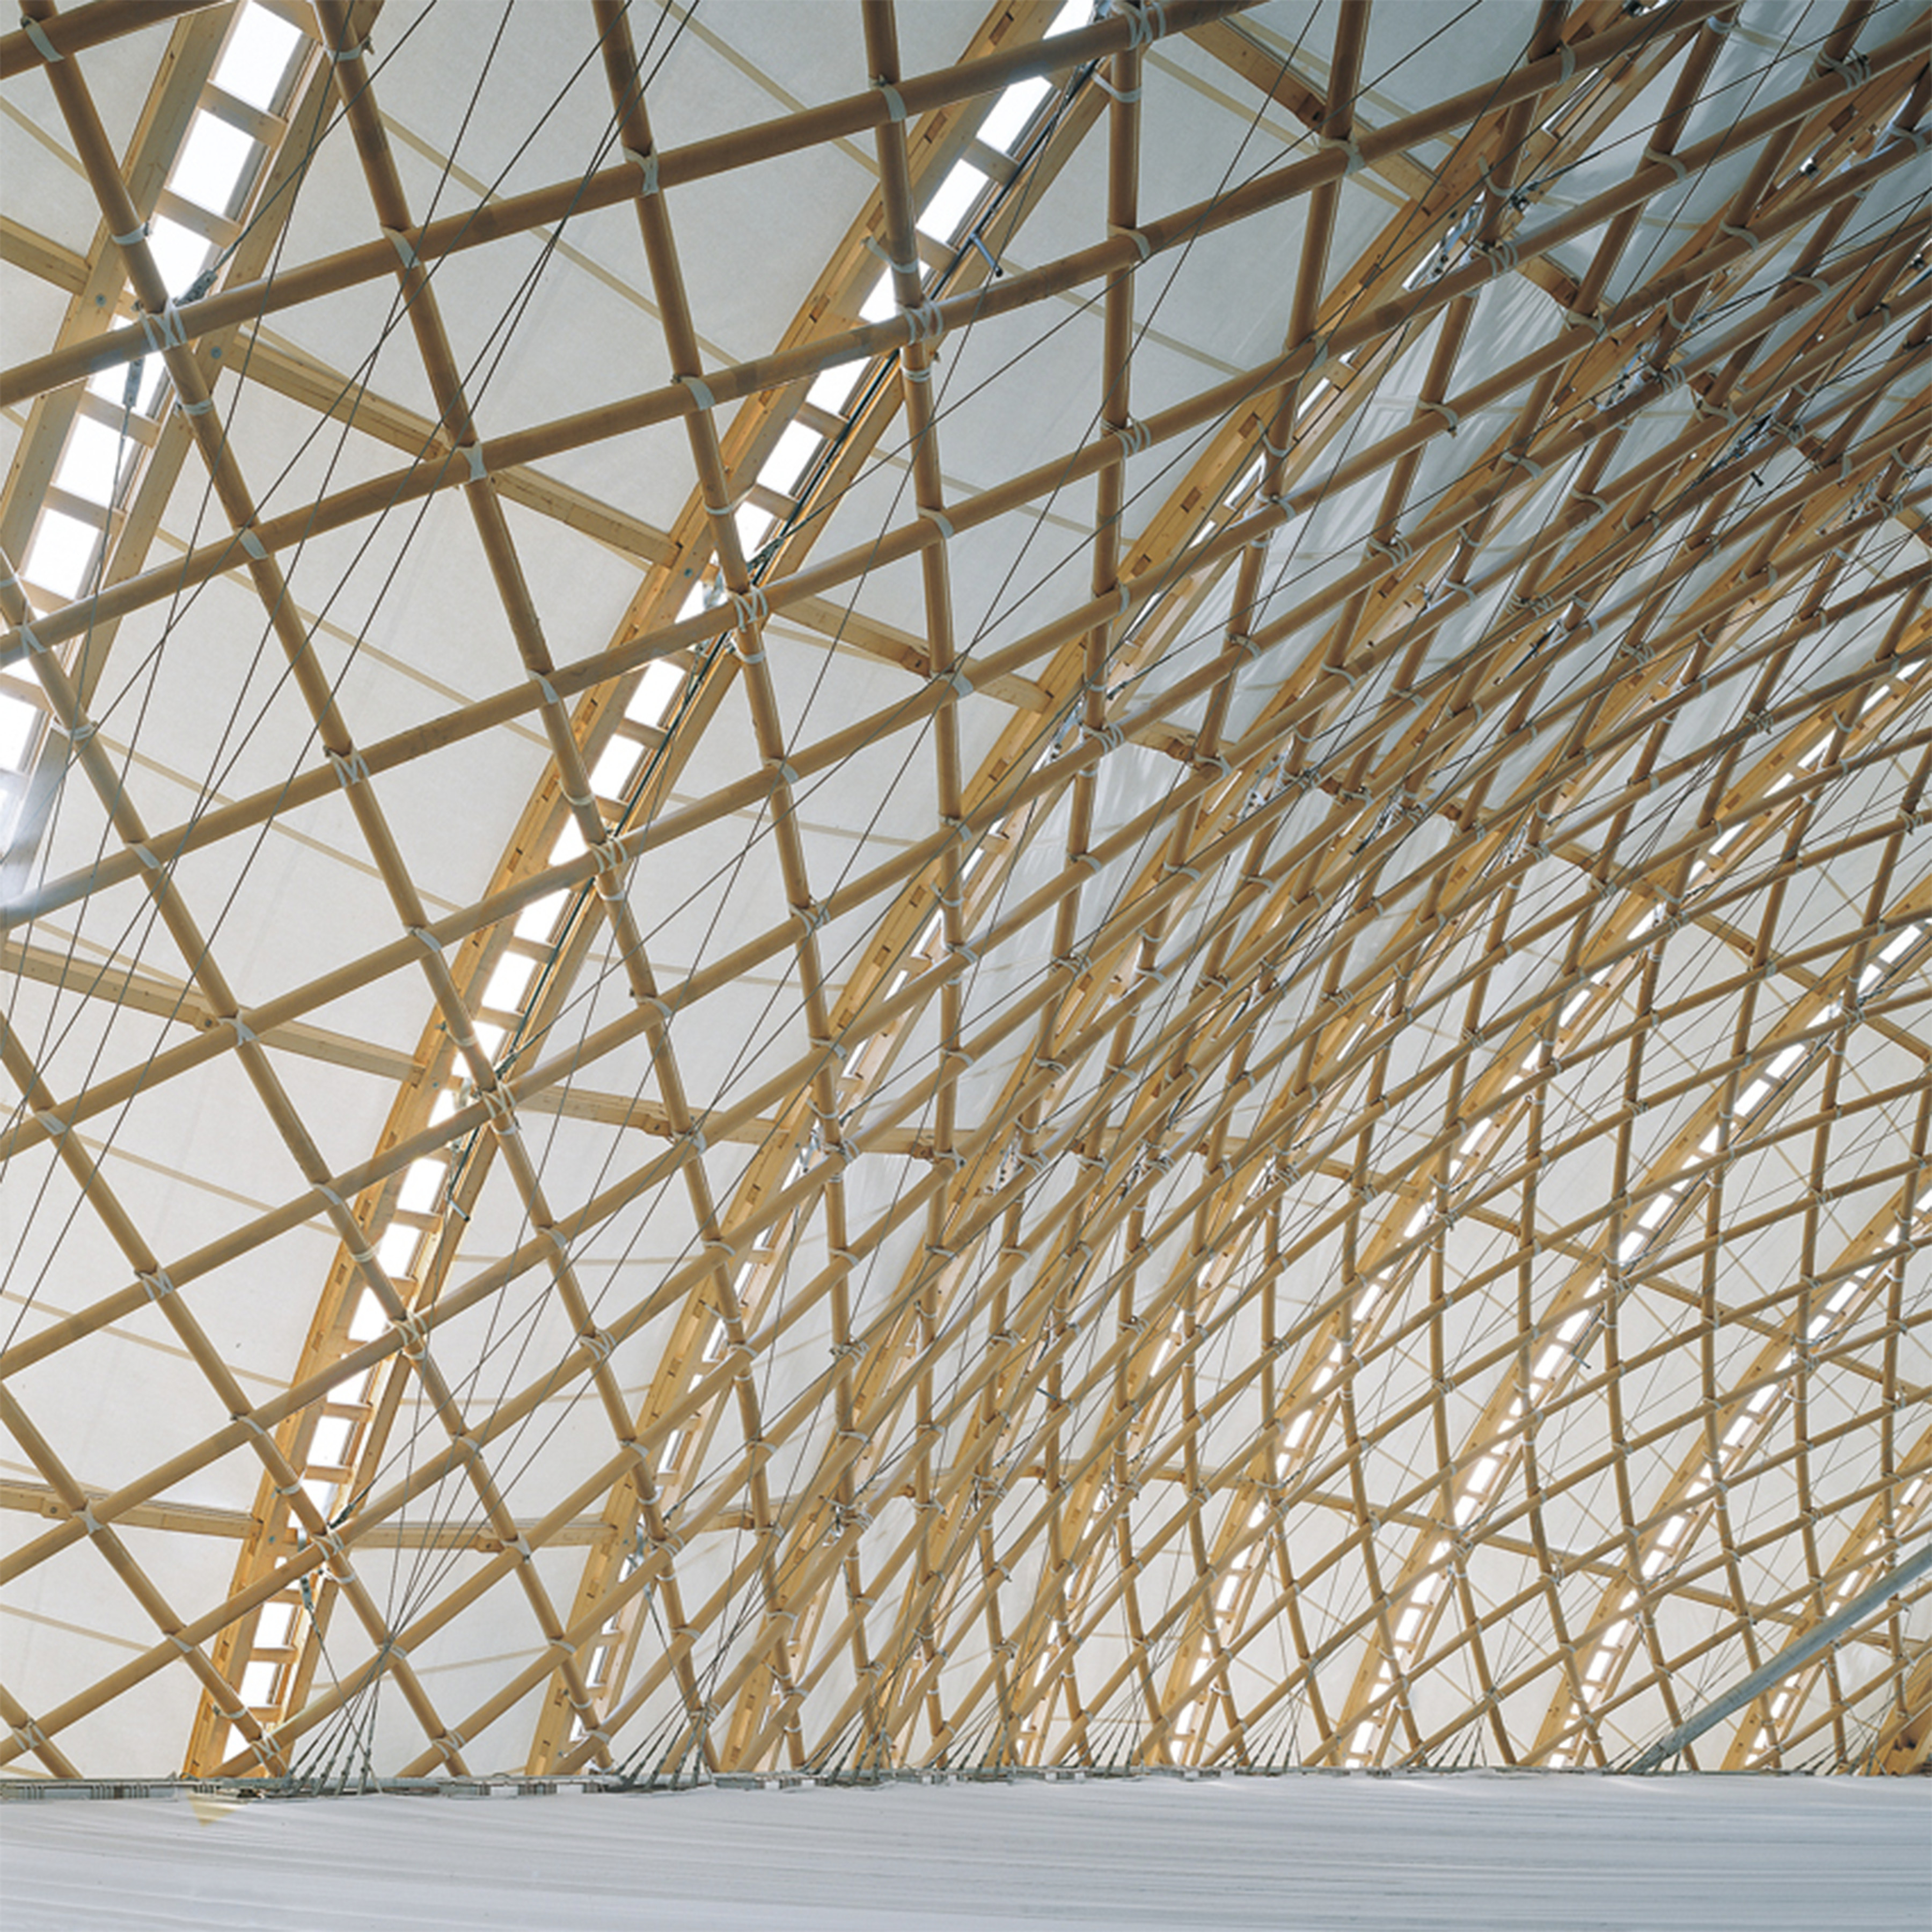
\includegraphics[width=0.32\MediaWidth]{hannover_int.jpg}\label{fig:hannover_a}}
%		\hspace*{\fill}
%		\subfloat[][Sky view]{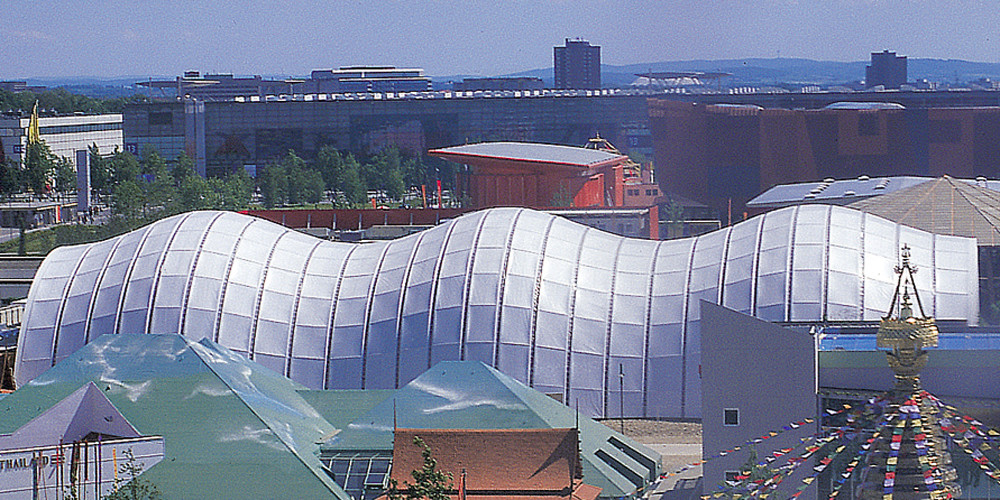
\includegraphics[width=0.64\MediaWidth]{hannover_sky.jpg}\label{fig:hannover_b}}
%%		\hrule
%		\captionof{figure}[Cardboard gridshell built in 2000 in Hannover, Germany]{Cardboard gridshell built in 2000 in Hannover, Germany.}\label{fig:hannover}
%		\hrule
%		\subfloat[][Interior view]{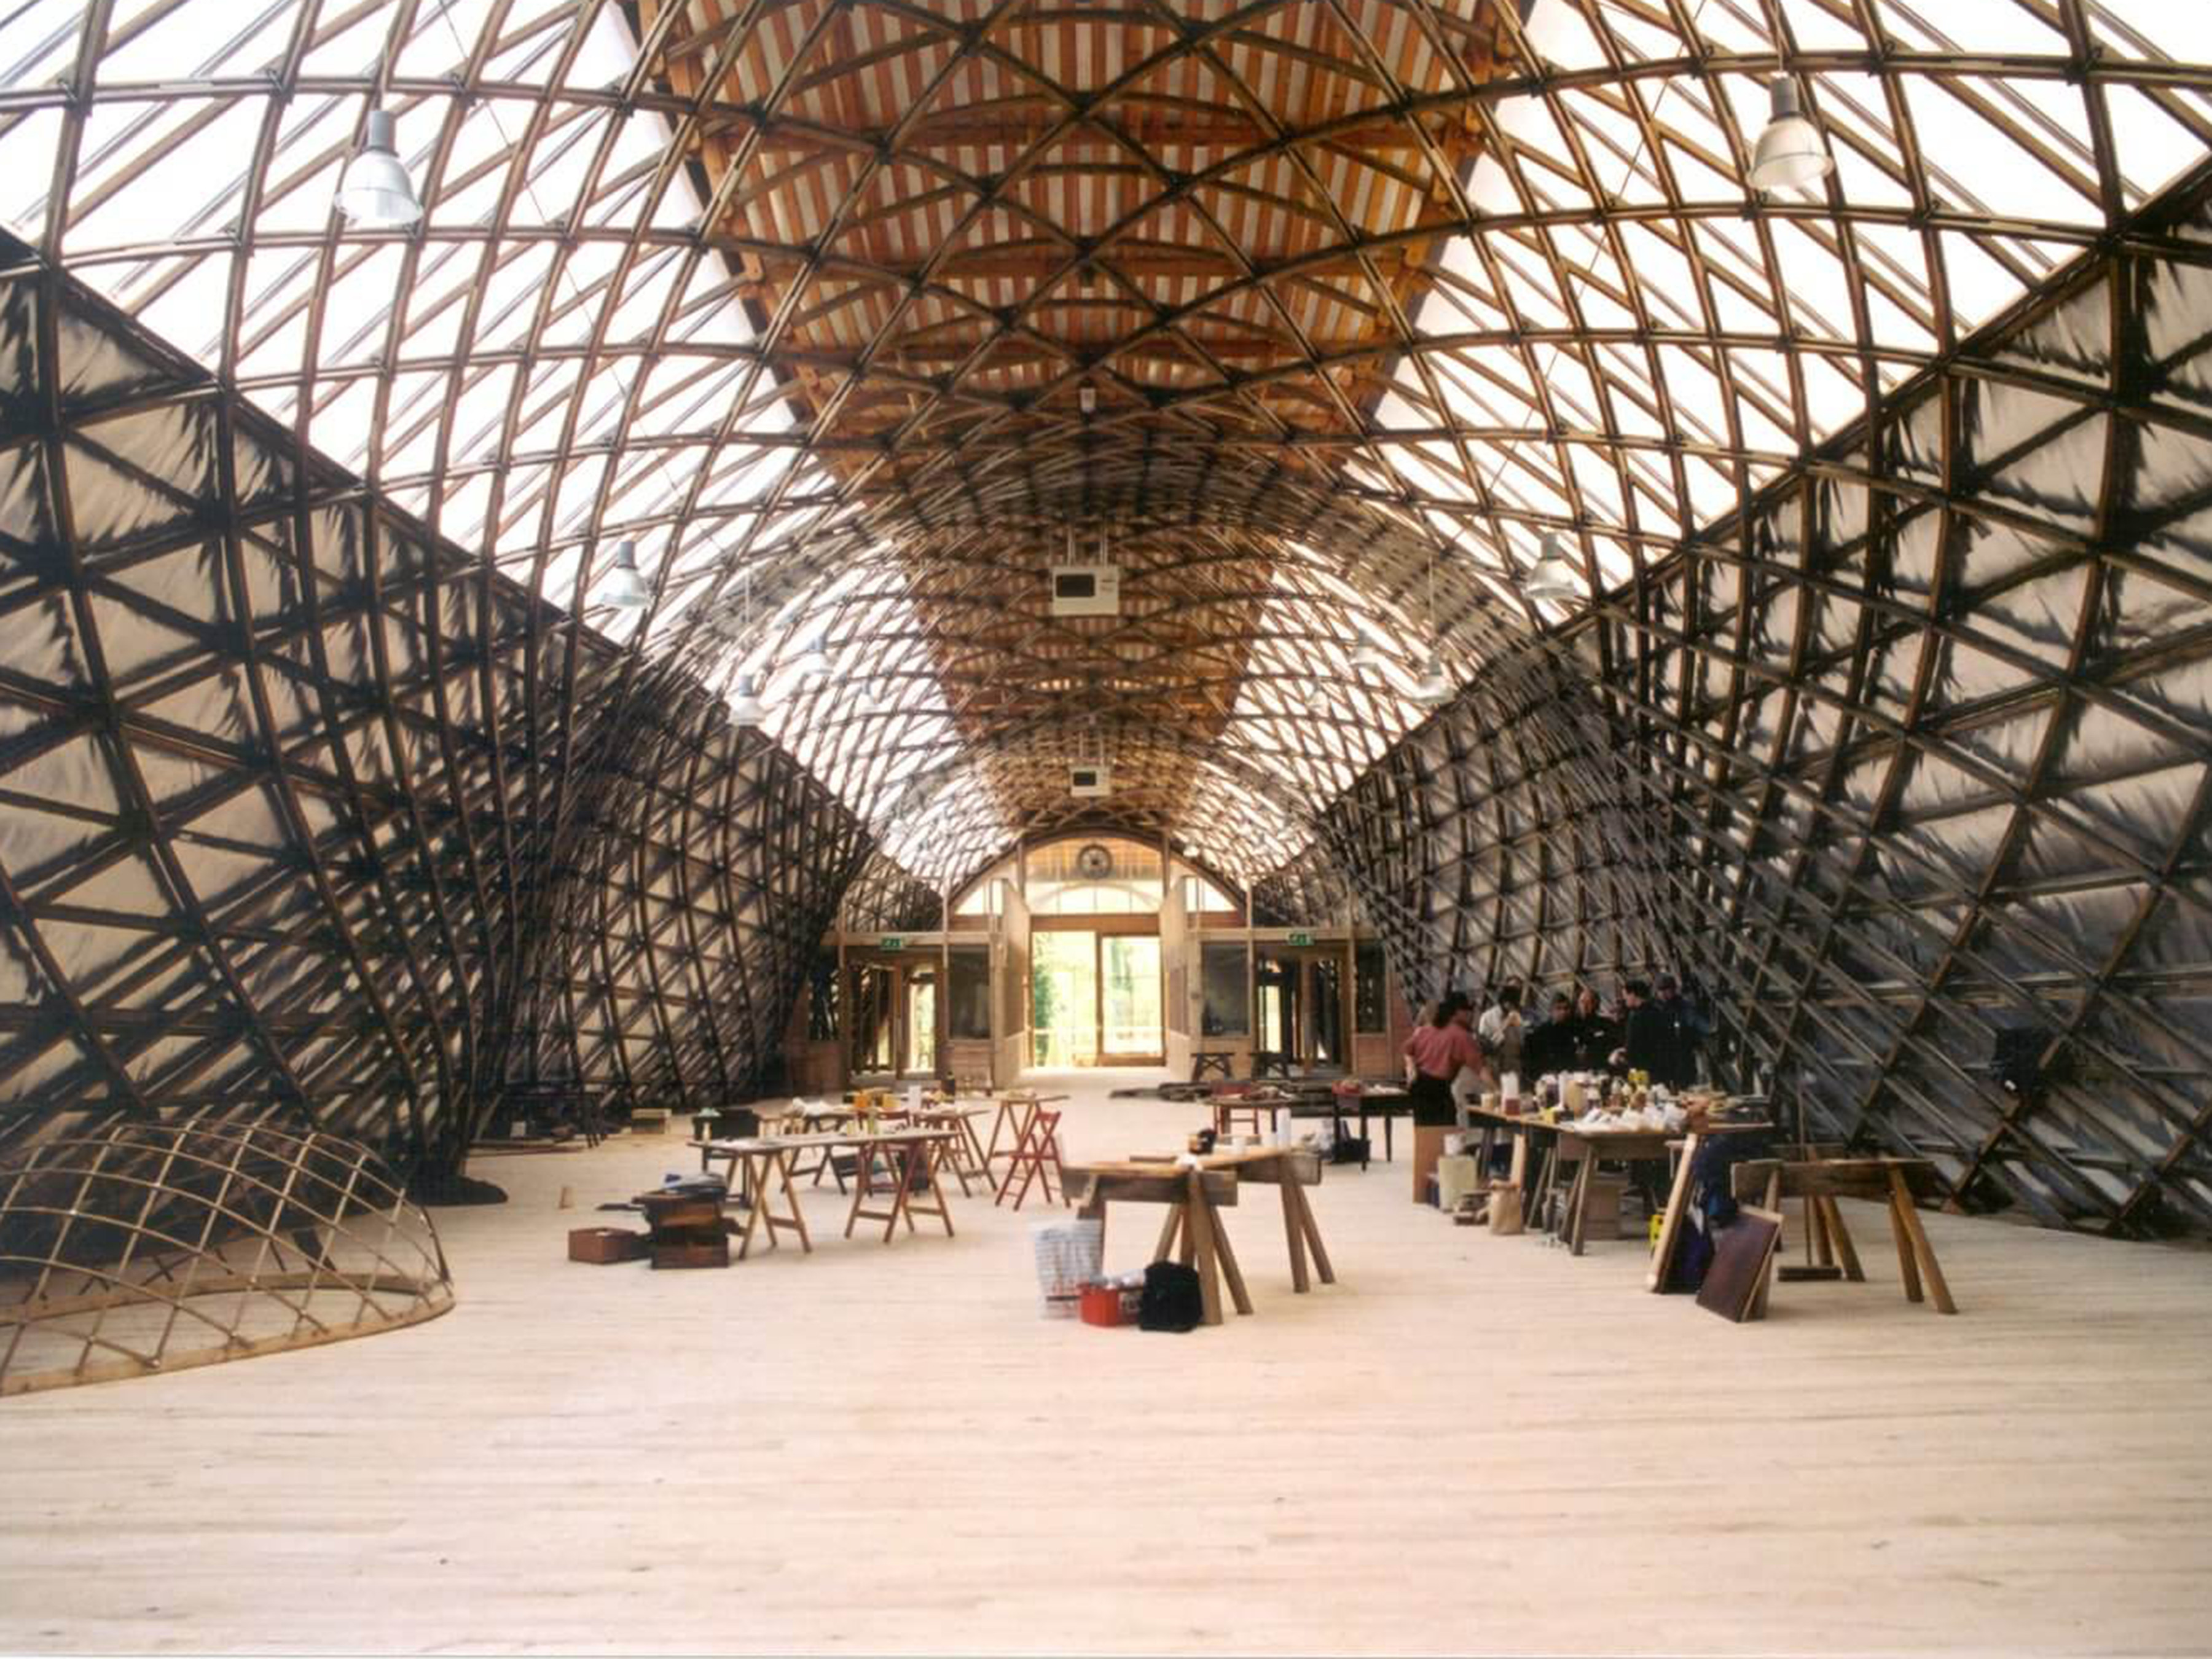
\includegraphics[width=0.48\MediaWidth]{downland_b.jpg}\label{fig:downland_a}}
%		\hspace*{\fill}
%		\subfloat[][Exterior view]{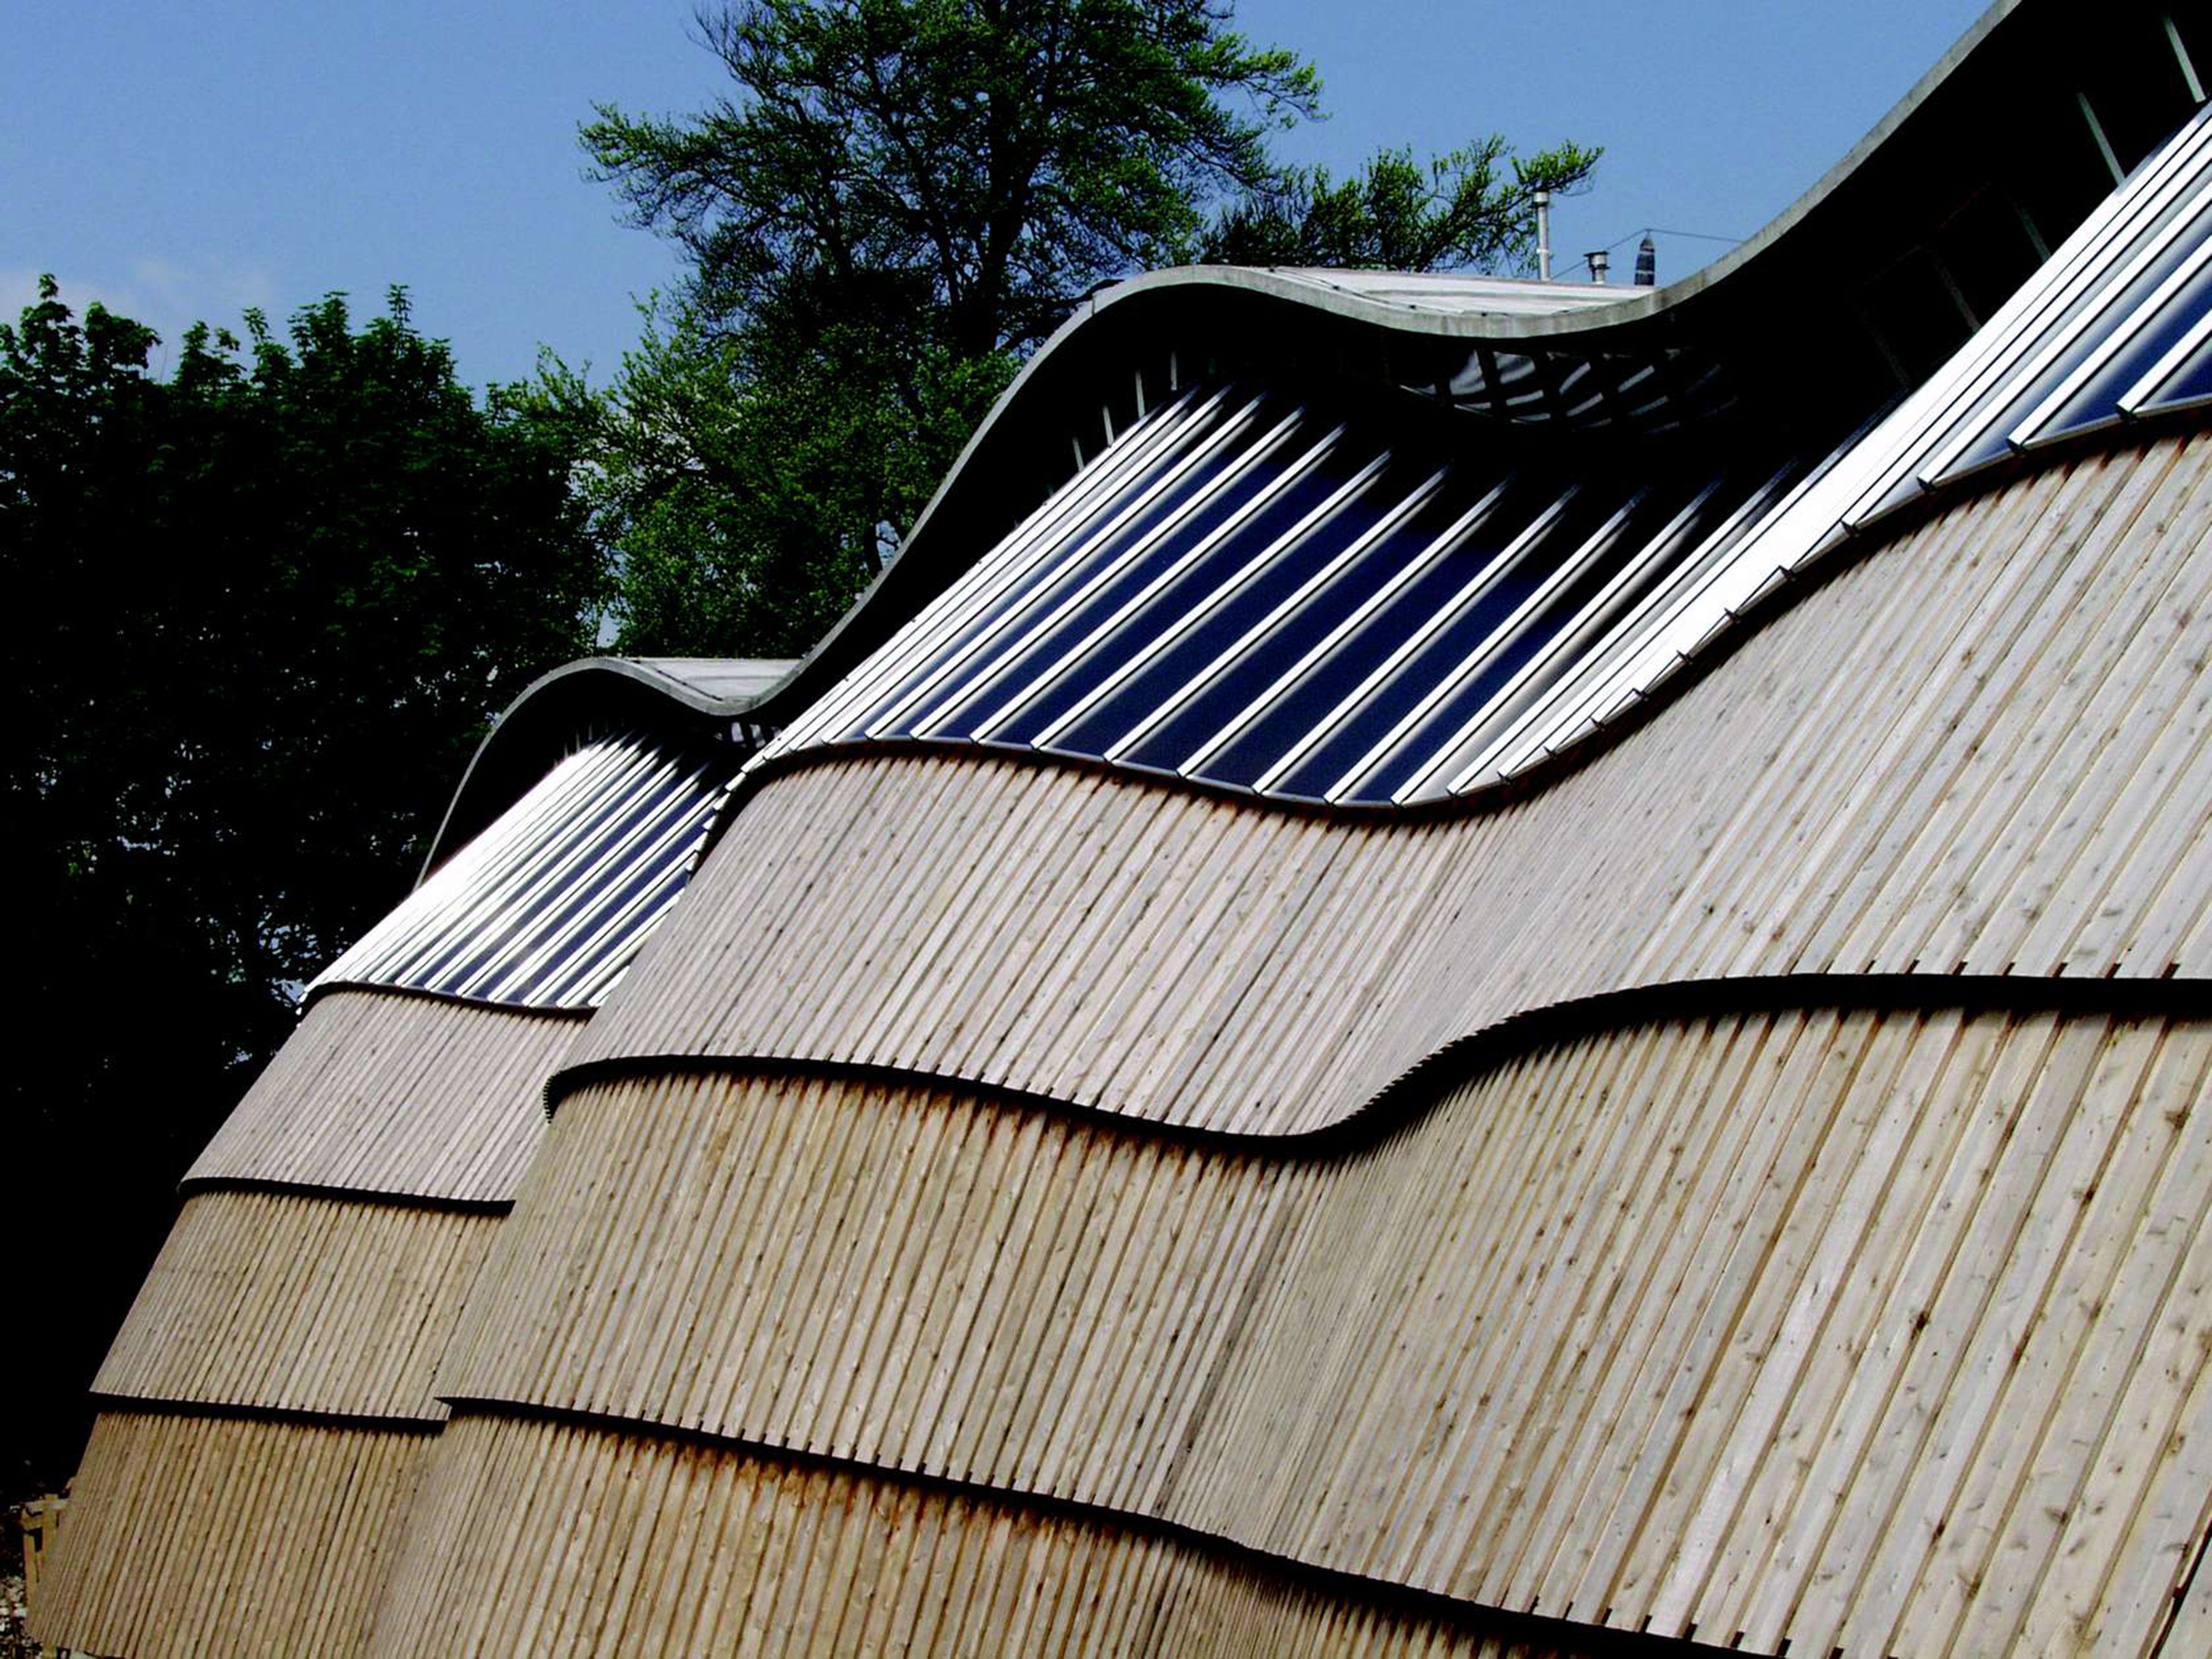
\includegraphics[width=0.48\MediaWidth]{downland_a.jpg}\label{fig:downland_b}}
%		\hrule
%		\captionof{figure}[Timber gridshell built in 2002 in Downland, England]{Timber gridshell built in 2002 in Downland, England.}\label{fig:downland}
%		\hrule
%%	\end{fullpage}
%\end{figure}

%\clearpage
%\begin{figure}[t]
%		\hrule
%		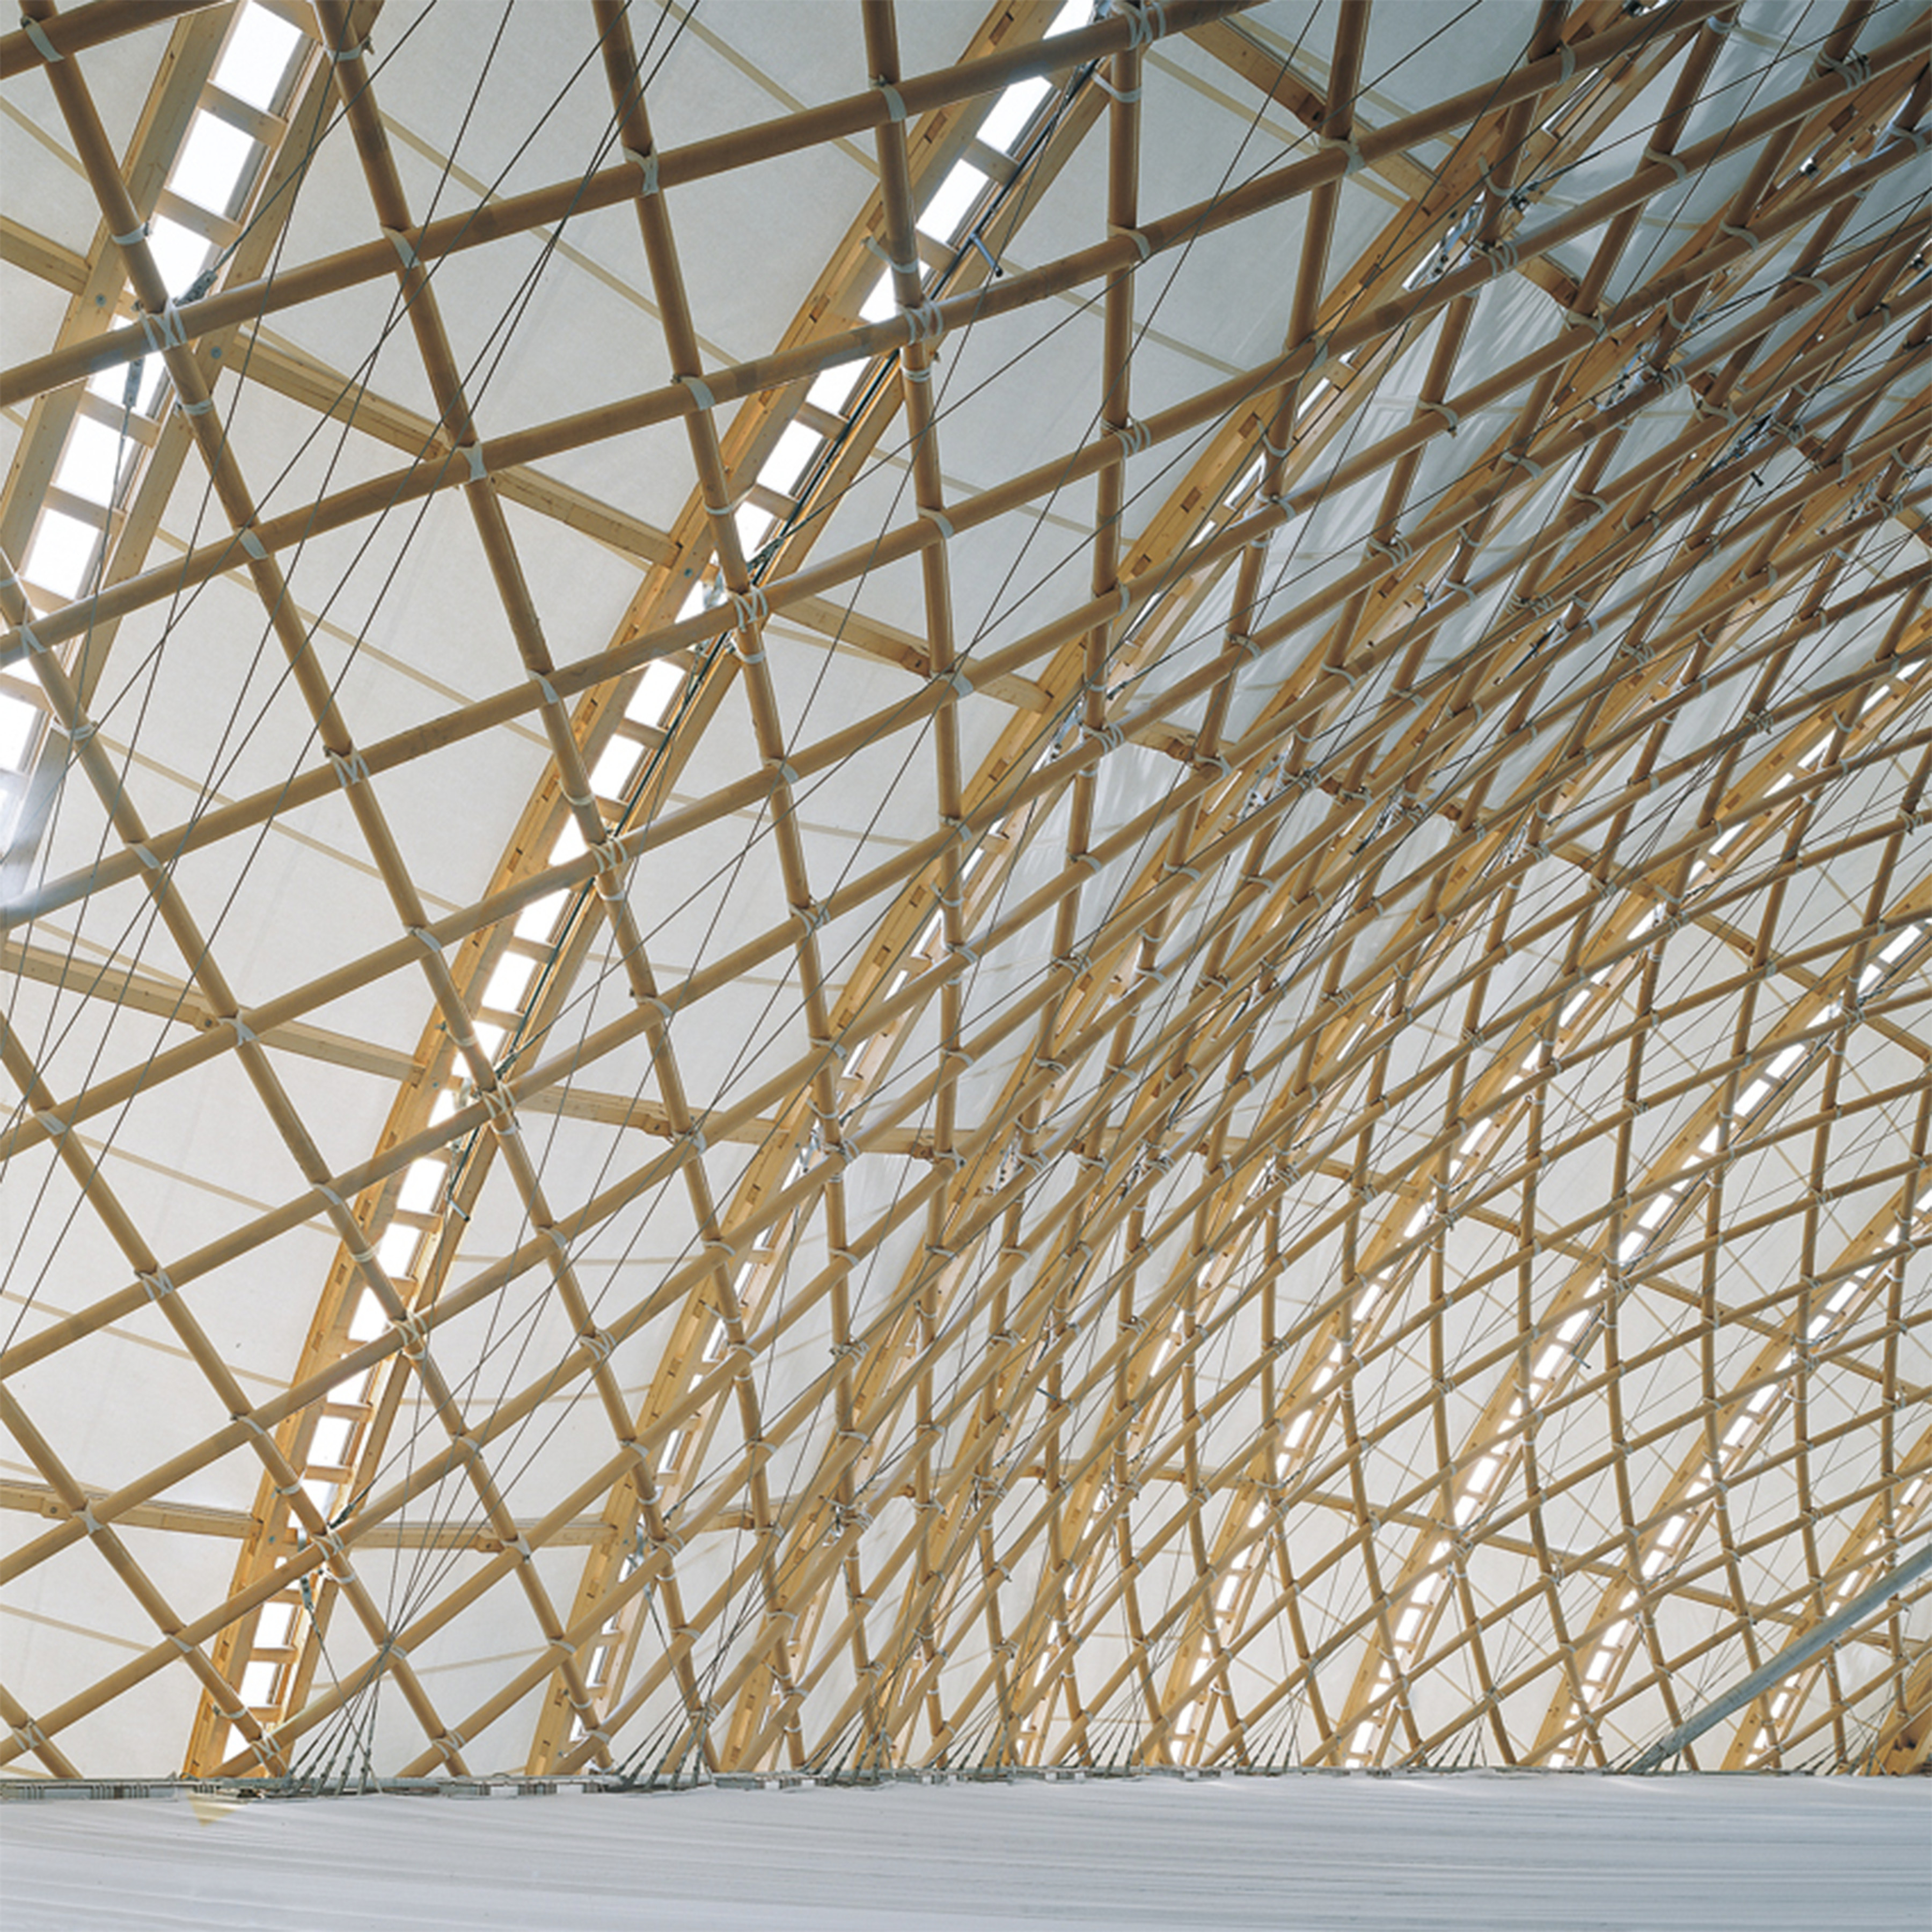
\includegraphics[width=0.32\MediaWidth]{hannover_int.jpg}
%		\hspace*{\fill}
%		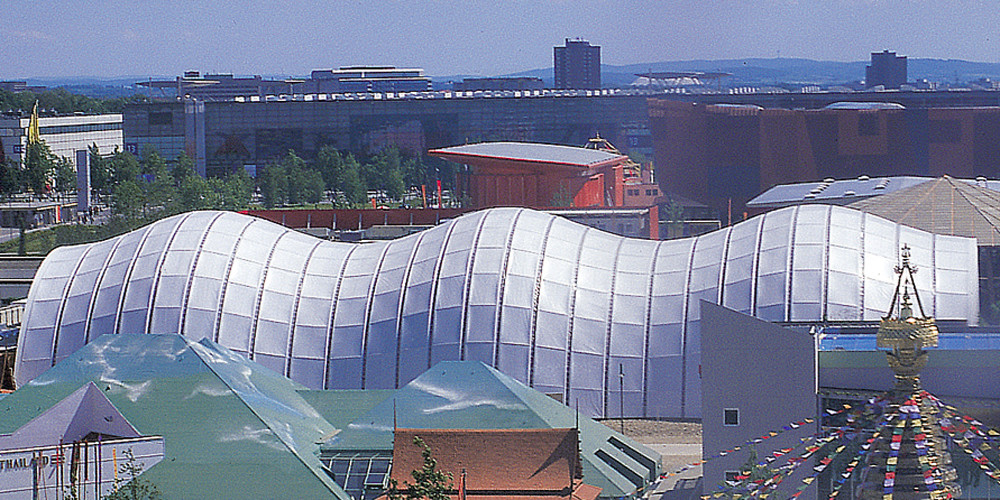
\includegraphics[width=0.64\MediaWidth]{hannover_sky.jpg}\label{fig:hannover_b}
%		\hrule
%		\captionof{figure}[Cardboard gridshell built in 2000 in Hannover, Germany]{Cardboard gridshell built in 2000 in Hannover, Germany.}
%		\hrule
%\end{figure}

%https://tex.stackexchange.com/questions/122314/figures-what-is-the-difference-between-using-subfig-or-subfigure/122329

\captionsetup{subrefformat=parens}

\begin{figure}[t]
\hrule
	\begin{subfigure}[b]{0.32\MediaWidth}
		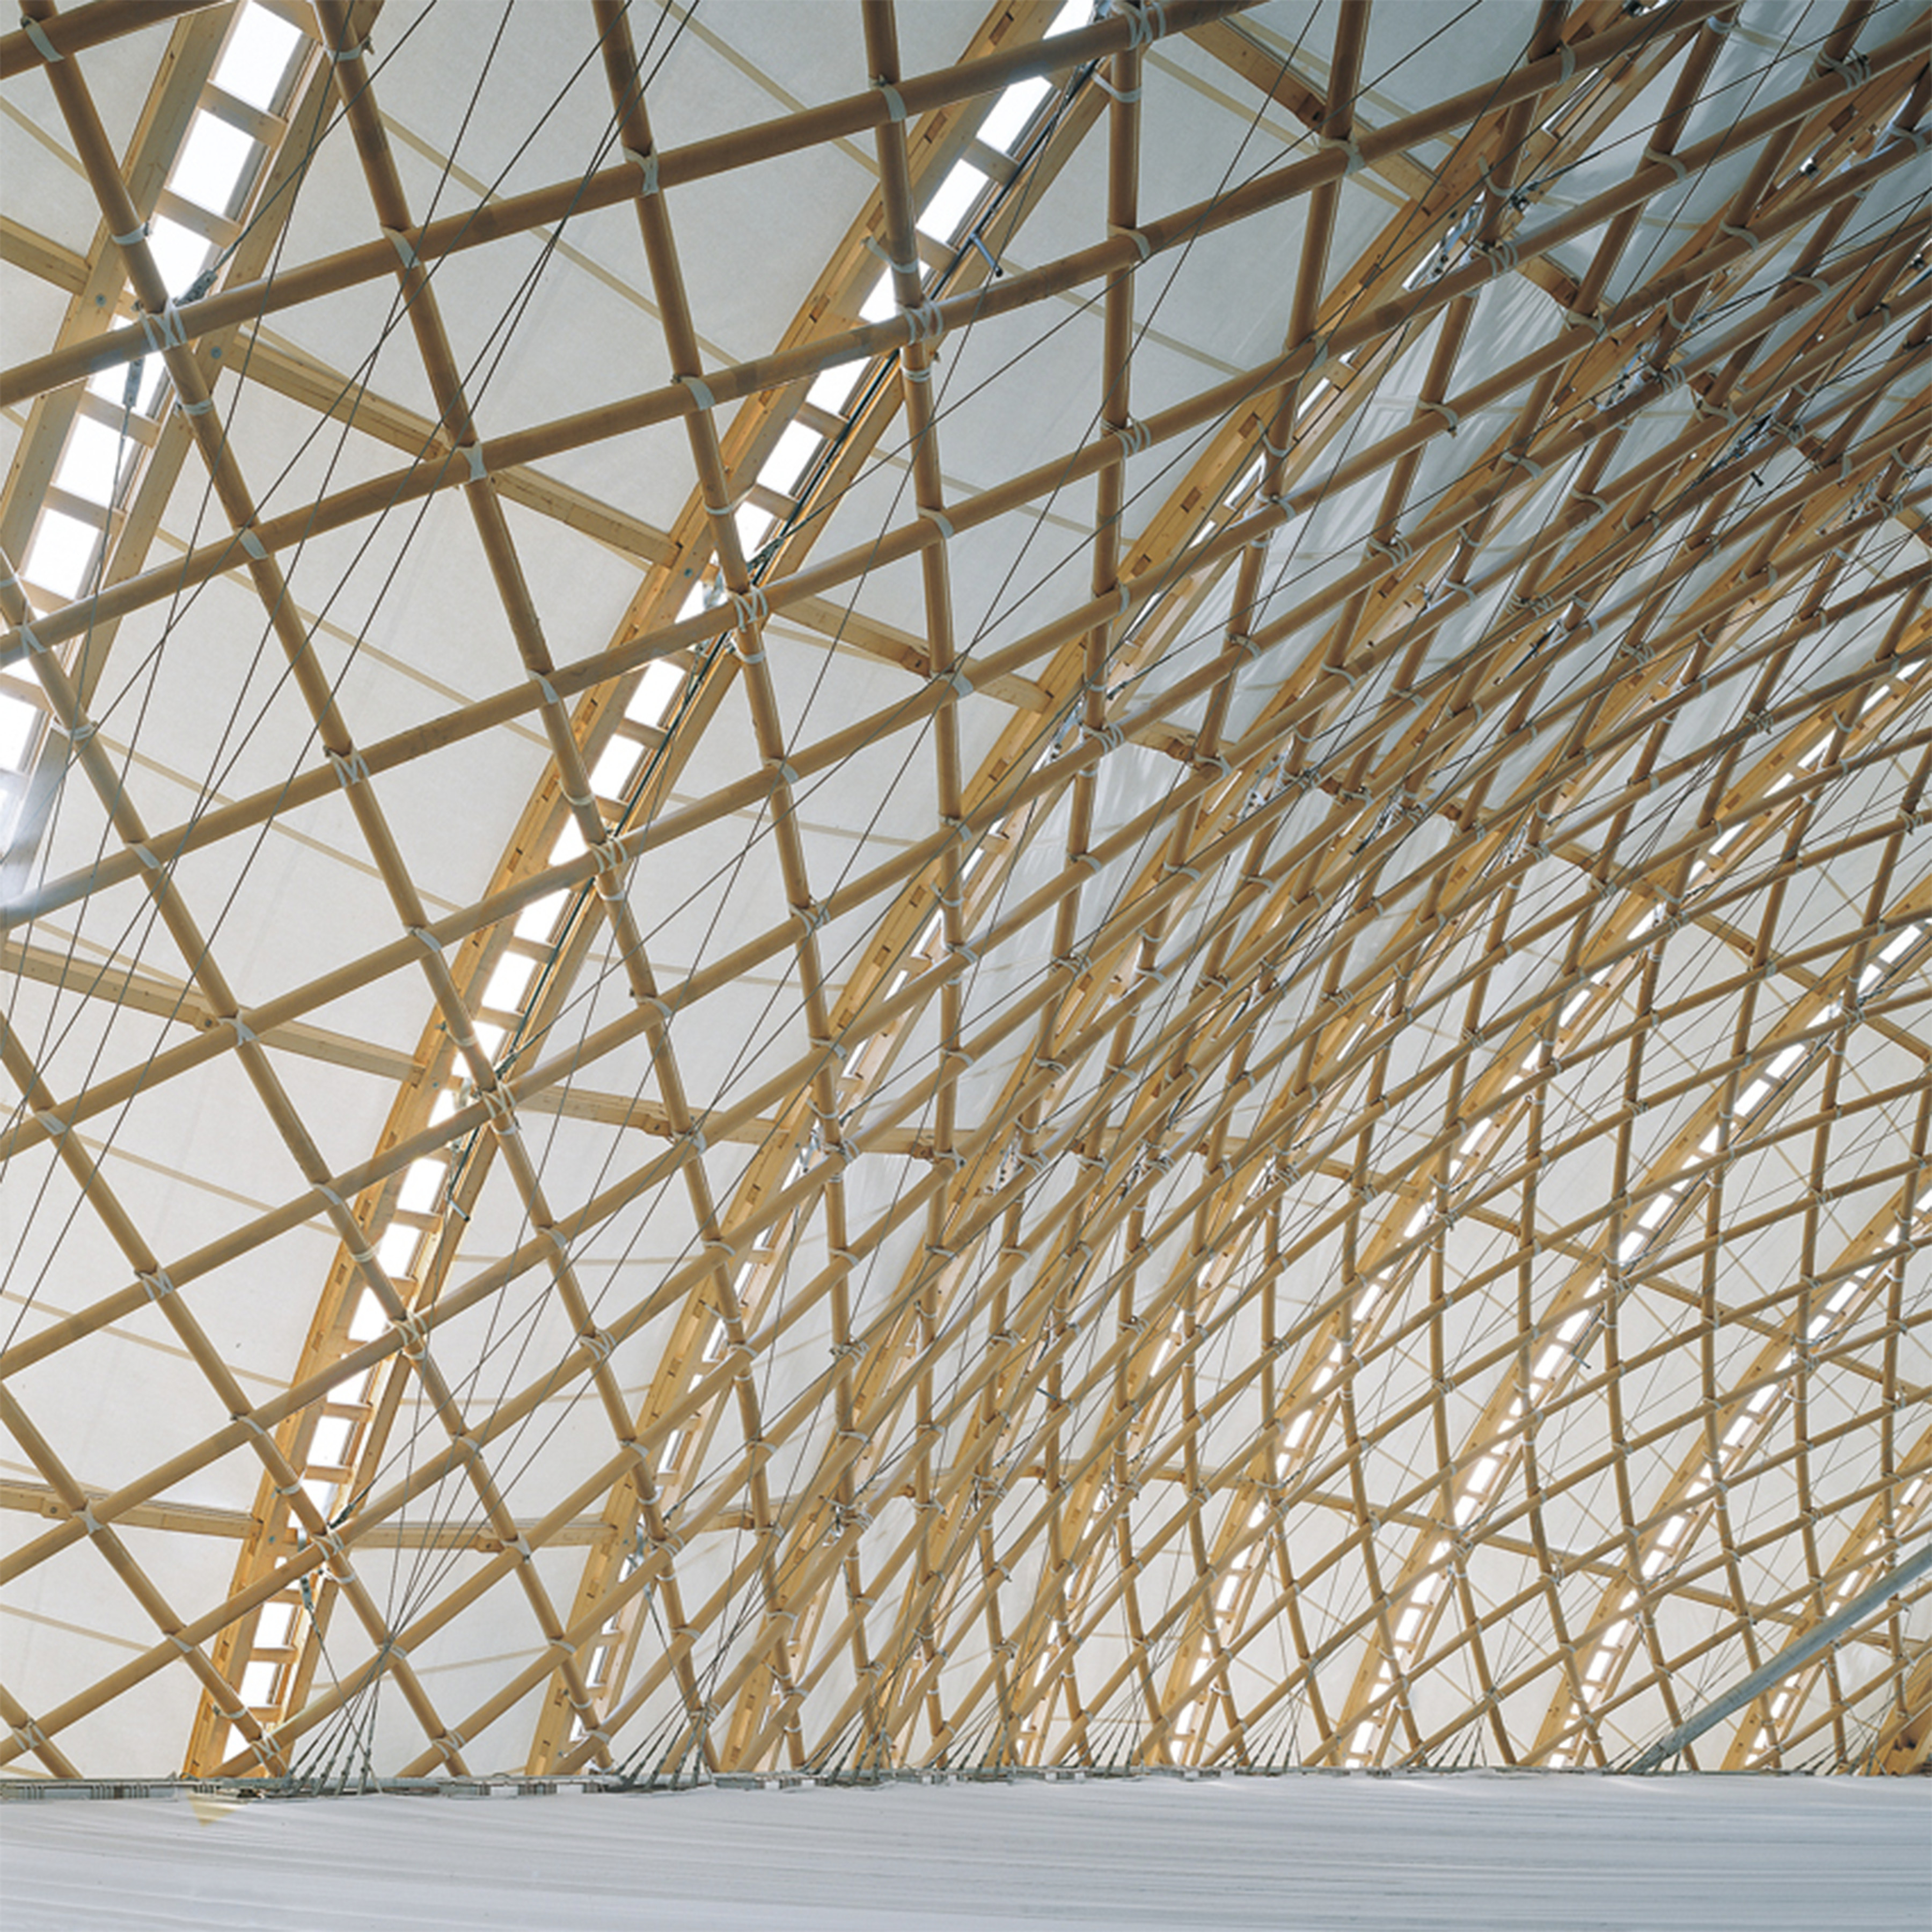
\includegraphics[width=\textwidth]{hannover_int.jpg}
		\caption{my first sub caption}
		\label{fig:hannover_a}
	\end{subfigure}
\hspace{\fill}%
	\begin{subfigure}[b]{0.64\MediaWidth}
		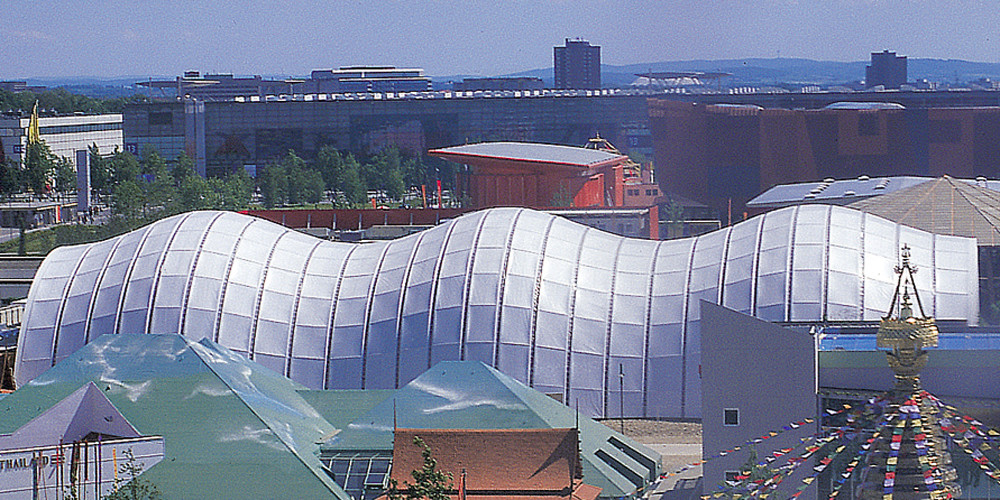
\includegraphics[width=\textwidth]{hannover_sky.jpg}
		\caption{my second sub caption}
		\label{fig:hannover_b}
	\end{subfigure}
\caption{Cardboard gridshell built in 2000 in Hannover, Germany.}
\label{fig:hannover}
\hrule
\end{figure}

smldksmldk

Main \cref{fig:hannover}, A \ref{fig:hannover_a}, B \ref{fig:hannover_b} 



The grid pitch is \SI{1.0}{m} except in weaker areas where it is \SI{0.5}{m}. There, the grid is twice denser to achieve the required buckling resistance \cite{Harris2003}. Rib-lath bracing was preferred to steel cable bracing as ribs were deemed to offer a more convenient support for the cladding and to reduce the complexity of the connection. A new connection system was developed to avoid the cost of drilling thousands of slotted holes that would, in addition, reduce the cross-section area, while maintaining the required scissor behaviour for the deformation of the timber lattice.\footnote{This detail was \href{https://patents.google.com/patent/GB2361504A/en?q=\%22A+coupling+and+a+method+of+constructing+grid+shell+buildings+using+such+a+coupling\%22&country=GB}{patented} by the design team and the client.}

The flat lattice was laid out on a scaffold platform. Unlike the Japan Pavilion, the lattice was progressively lowered down into position. This stage took 6 weeks. Once deformed, the shear blocks were introduced in the grid and bracing rib-laths were installed, giving its full strength to the shell. Finally the gridshell was cladded with a mix of polycarbonate plates (to let the light in) and timber boards on top of insulation panels and a rain screen.

It is worthwhile to mention that for the first time the form was not found by inverting some sort of hanging chain model that would produce a pure funicular shape where only compression occurred. Instead, the shape was the result of a numerical computation that took into account the bending behaviour of the laths.\footnote{This software was developed under the supervision of Chris Williams of the university of Bath.} \citet{Harris2003} argued that computer models enabled some interactivity in the form-finding process that would not be possible with physical models, leading to a better synergy between architectural and structural requirements. They also argued that physical models contributed invaluably to the development of a creative and efficient design throughout the project.

\subsubsection{Lothian Gridshell, Pishwanton, Scotland, 2002}
This project deserves some attention because the developed approach was completely different from the projects exposed until now~: \blockcquote[]{Lowenstein2002}{Previous projects have portrayed the method as a highly technical use of a low-tech resources. This, however, needs not be the case as we see with this project \belp{}}. The structure was the result of \blockcquote[]{bdonline2002}{\belp{} an unusual collaboration between sole practitioner Christopher Day, engineer David Tasker, a crowd of local volunteers and (more unusually) the philosophies of Rudolf Steiner and Johann Wolfgang Goethe}.\footnote{From the online paper \textquote{The other gridshell} : \url{http://www.bdonline.co.uk/the-other-gridshell/1020435.article}}

The single-layer gridshell was made out of local larch. Once erected by hands, the dome-like shape covered about \SI{80}{m^2} and spanned 10 meters. The grid was braced with timber boards (see \cref{fig:pishwanton_a}) and covered with a planted turf roof (see \cref{fig:pishwanton_b}). Some calculations were made but in the end, it had to carry load testing to prove its safety and gain its regulation approval.\footnote{\blockcquote[]{bdonline2002}{There were a lot of calculations but no computer-generated models to show they all added up. In fact, the form was previously established with scale models. When it came to gaining Building Regulations approval, the team needed to prove that the building would be strong enough. So Tasker arranged for the unfinished structure to be loaded with about 18 tonnes of sand from a local quarry – equivalent to the maximum predicted snow load, plus a safety factor.}}

\subsubsection{Woodland Centre, Filmwell, England, 2003}
The gridshell of the Woodland Centre was built 7 years after the project had started (see \cref{fig:flimwell_a}).\footnote{More to be found at : \href{http://www.fourthdoor.org/annular/?page_id=441}{Growing and making Flimwell’s chestnut gridshell}.} The building was designed by architect Feilden Clegg and engineers from Atelier One. It was part of a larger research and development project that aimed at developing chestnut -- a low grad wood -- as a construction material.\footnote{This projet was conducted by the \href{http://www.bre.co.uk/}{Building Research Establishment}.}

The building, still existing, is composed of 5 barrel vaults spanning 12 meters and about 5 meters wide (see \cref{fig:flimwell_b}). It covers about \SI{300}{m^2} \cite{Lowenstein2004}. Each vault module is a transportable unit composed of two curved arches. A single layer gridshell was then applied to this primary frame and braced with chestnut panels. The grid was made of laths with~\SI{75}{mm} x \SI{25}{mm} rectangular cross-section, assembled with simple bolts. On top of that, insulation materials and a membrane as rainscreen \cite{FourthDoor2003}.

\begin{figure}[t]
	% (%) required at end of lines to prevent extra space
	\hrule
	%
	%
	\begin{subfigure}[b]{\TwoMediaWidth}
		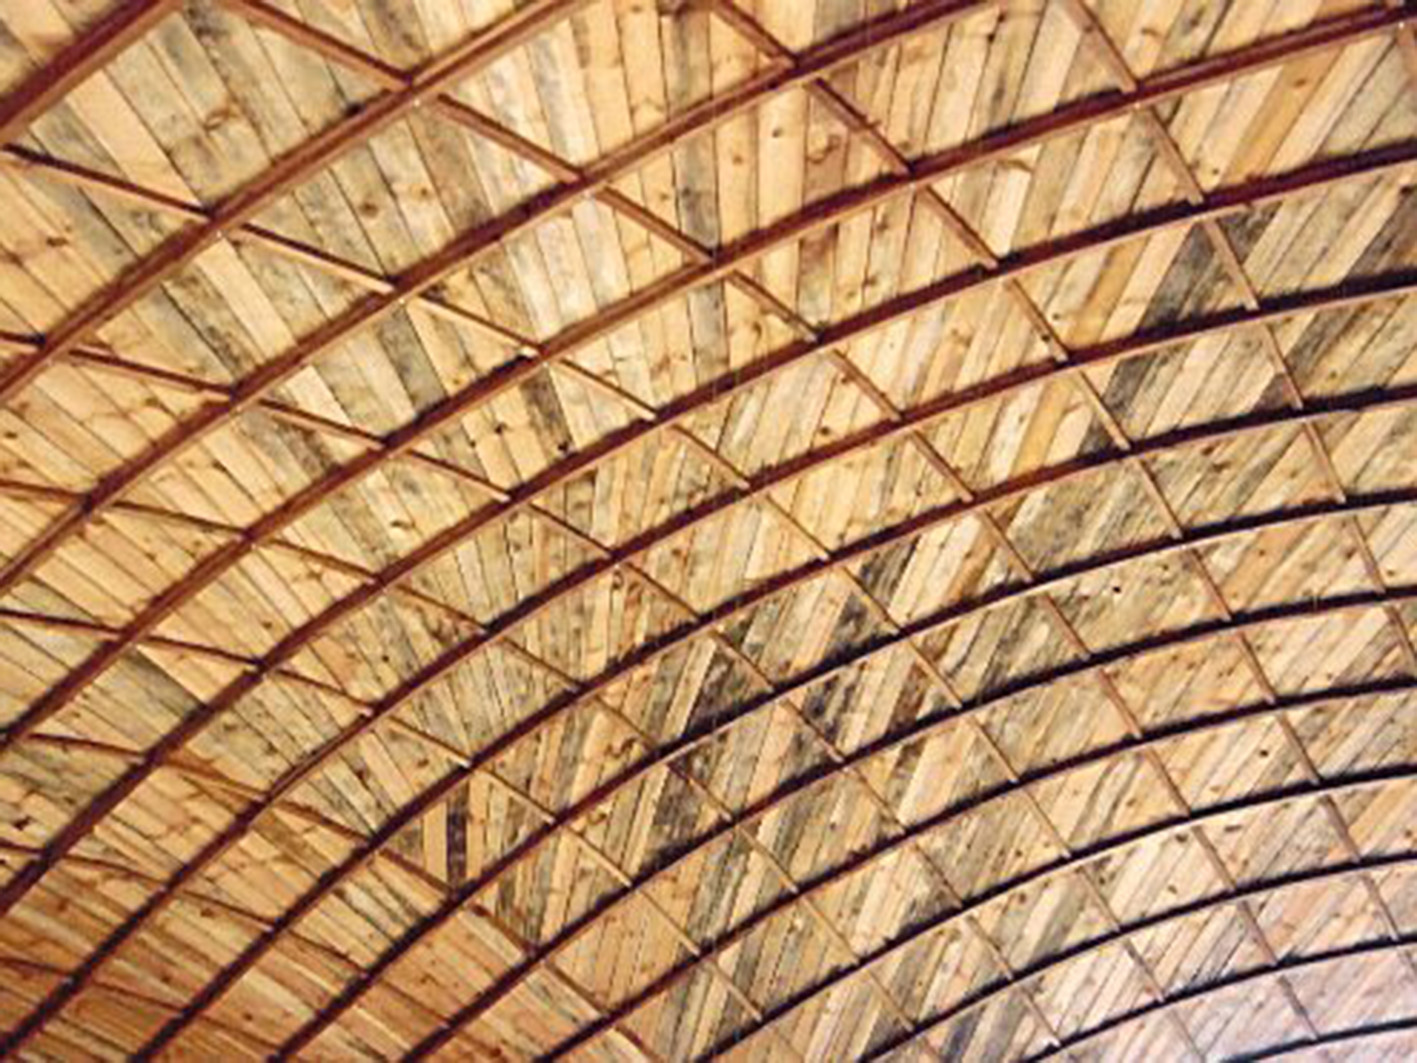
\includegraphics[width=\textwidth]{pishwanton_int.jpg}
		\caption{Interior view}
		\label{fig:pishwanton_a}
	\end{subfigure}%
	\hspace{\MediaGutterWidth}%
	\begin{subfigure}[b]{\TwoMediaWidth}
		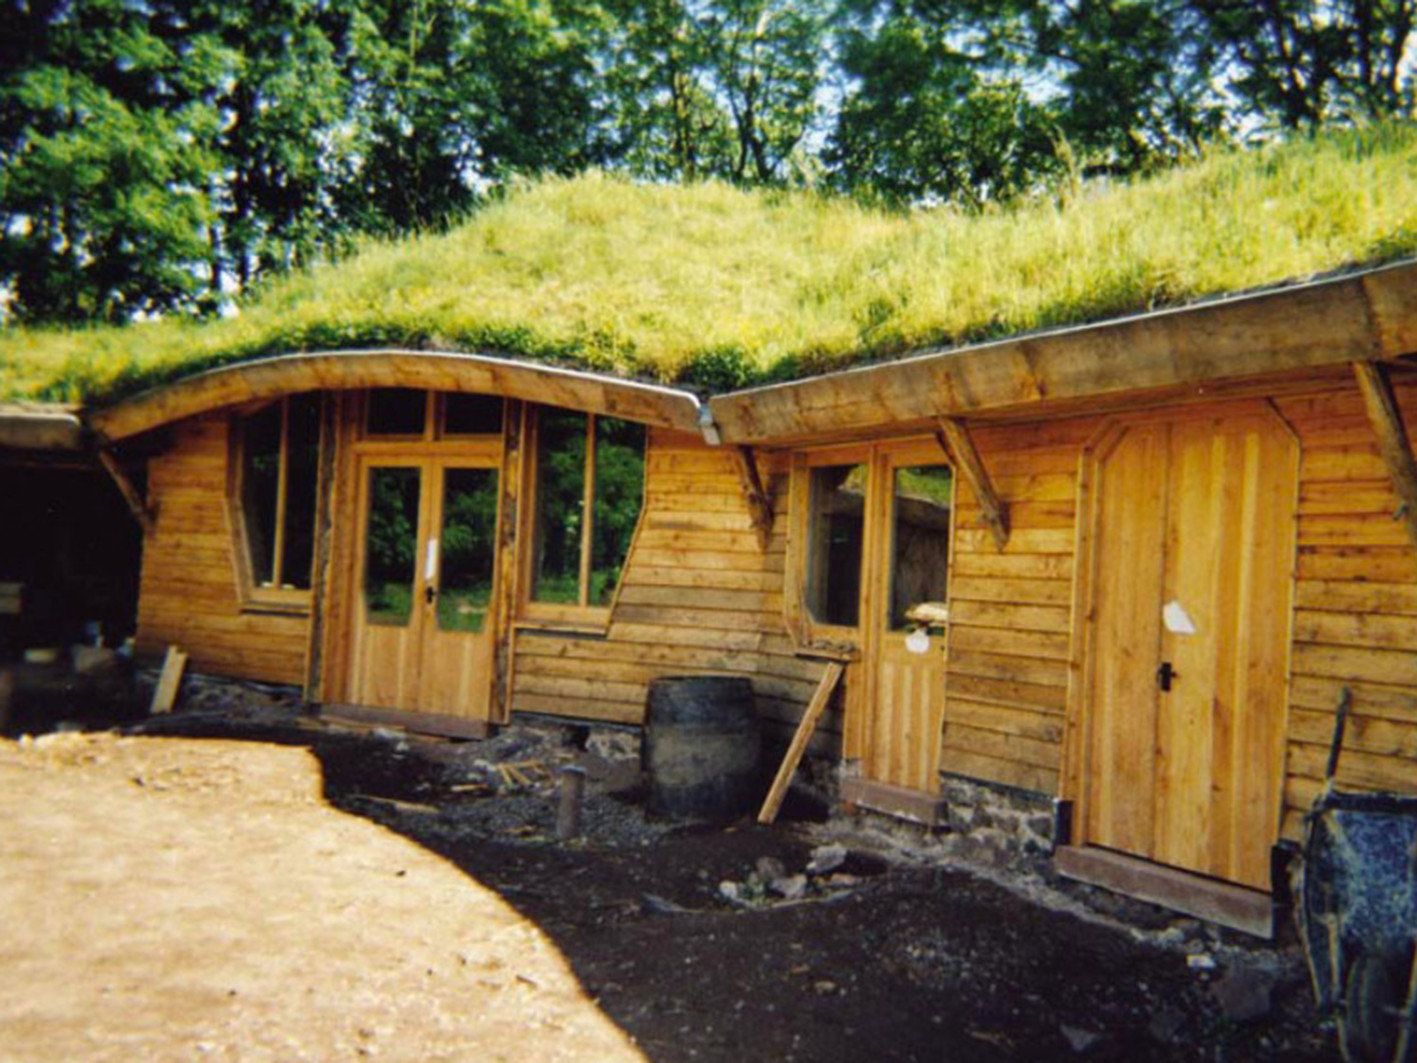
\includegraphics[width=\textwidth]{pishwanton_ext.jpg}
		\caption{Exterior view}
		\label{fig:pishwanton_b}
	\end{subfigure}
	\caption[Timber gridshell built in 2002 in Pishwanton, England]{Timber gridshell built in 2002 in Pishwanton, England.}
	\label{fig:pishwanton}
	%
	\subfigskip
	%
	\begin{subfigure}[b]{\TwoMediaWidth}
		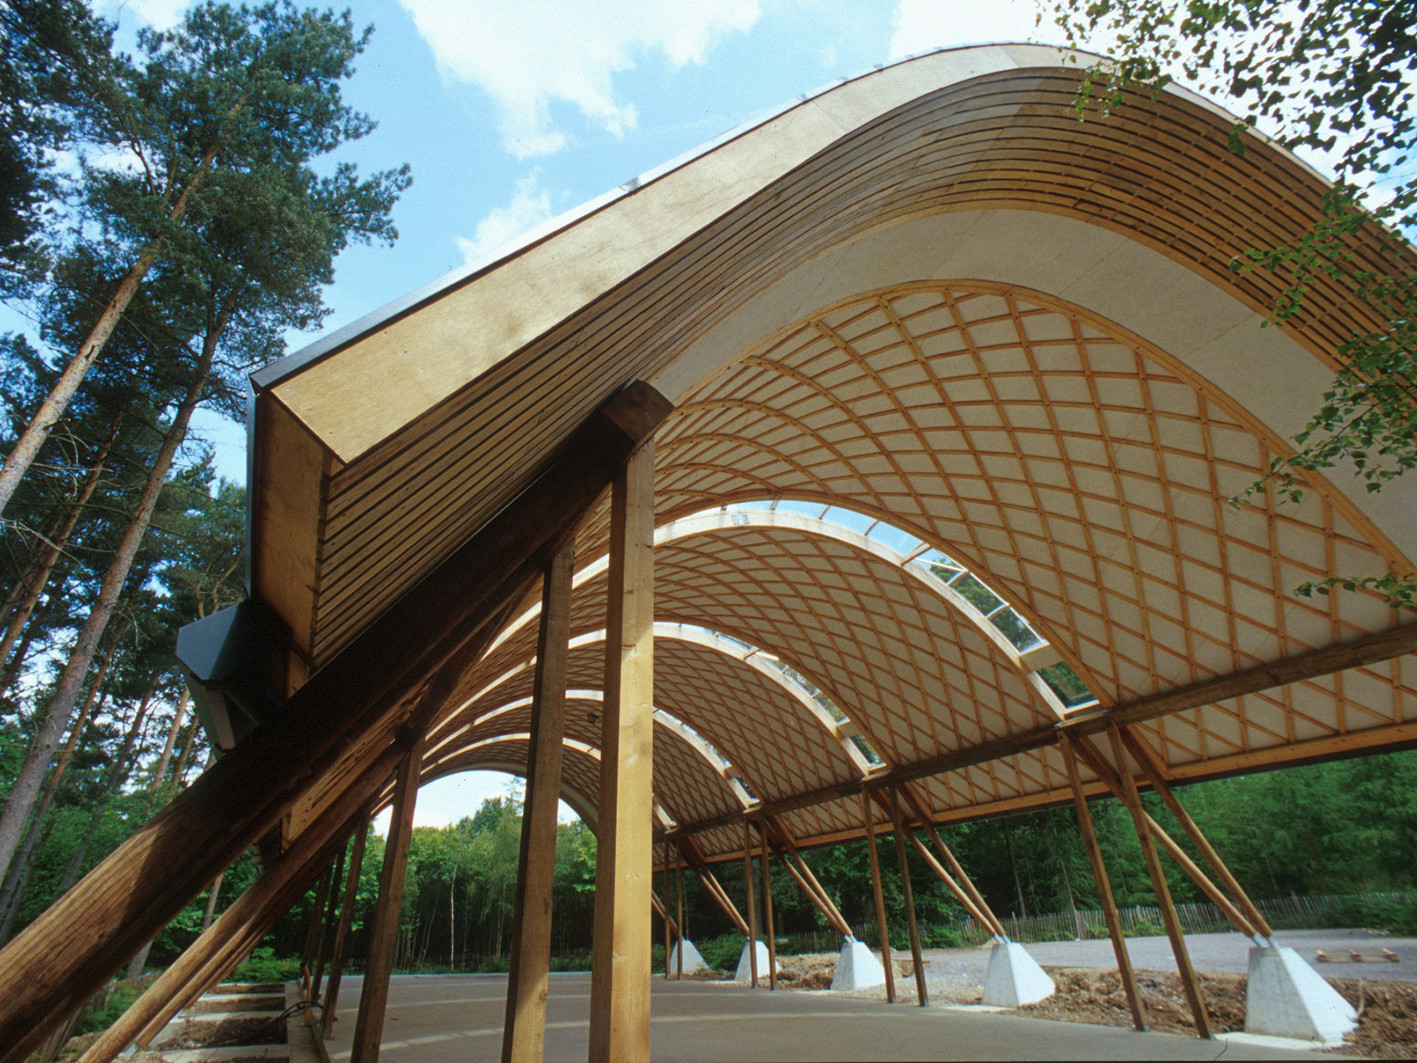
\includegraphics[width=\textwidth]{flimwell_int.jpg}
		\caption{Interior view}
		\label{fig:flimwell_a}
	\end{subfigure}%
	\hspace{\MediaGutterWidth}%
	\begin{subfigure}[b]{\TwoMediaWidth}
		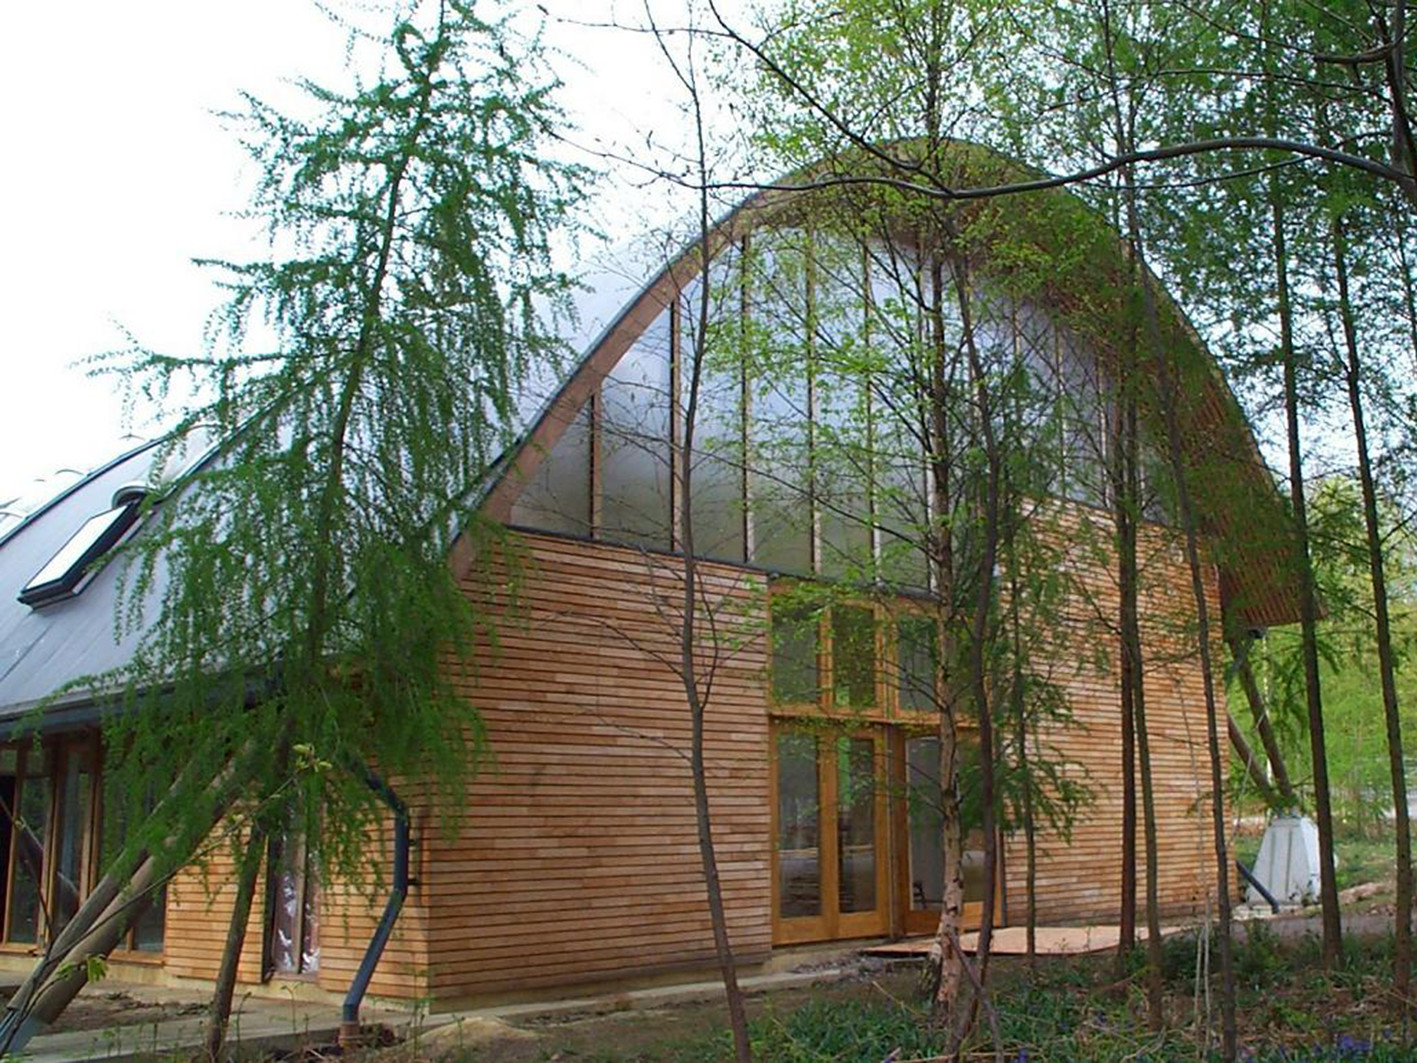
\includegraphics[width=\textwidth]{flimwell_ext.jpg}
		\caption{Exterior view}
		\label{fig:flimwell_b}
	\end{subfigure}
	\caption[Timber gridshell built in 2003 in Filmwell, England]{Timber gridshell built in 2003 in Filmwell, England.}
	\label{fig:flimwell}
	%
	\subfigskip
	%
	\begin{subfigure}[b]{\TwoMediaWidth}
		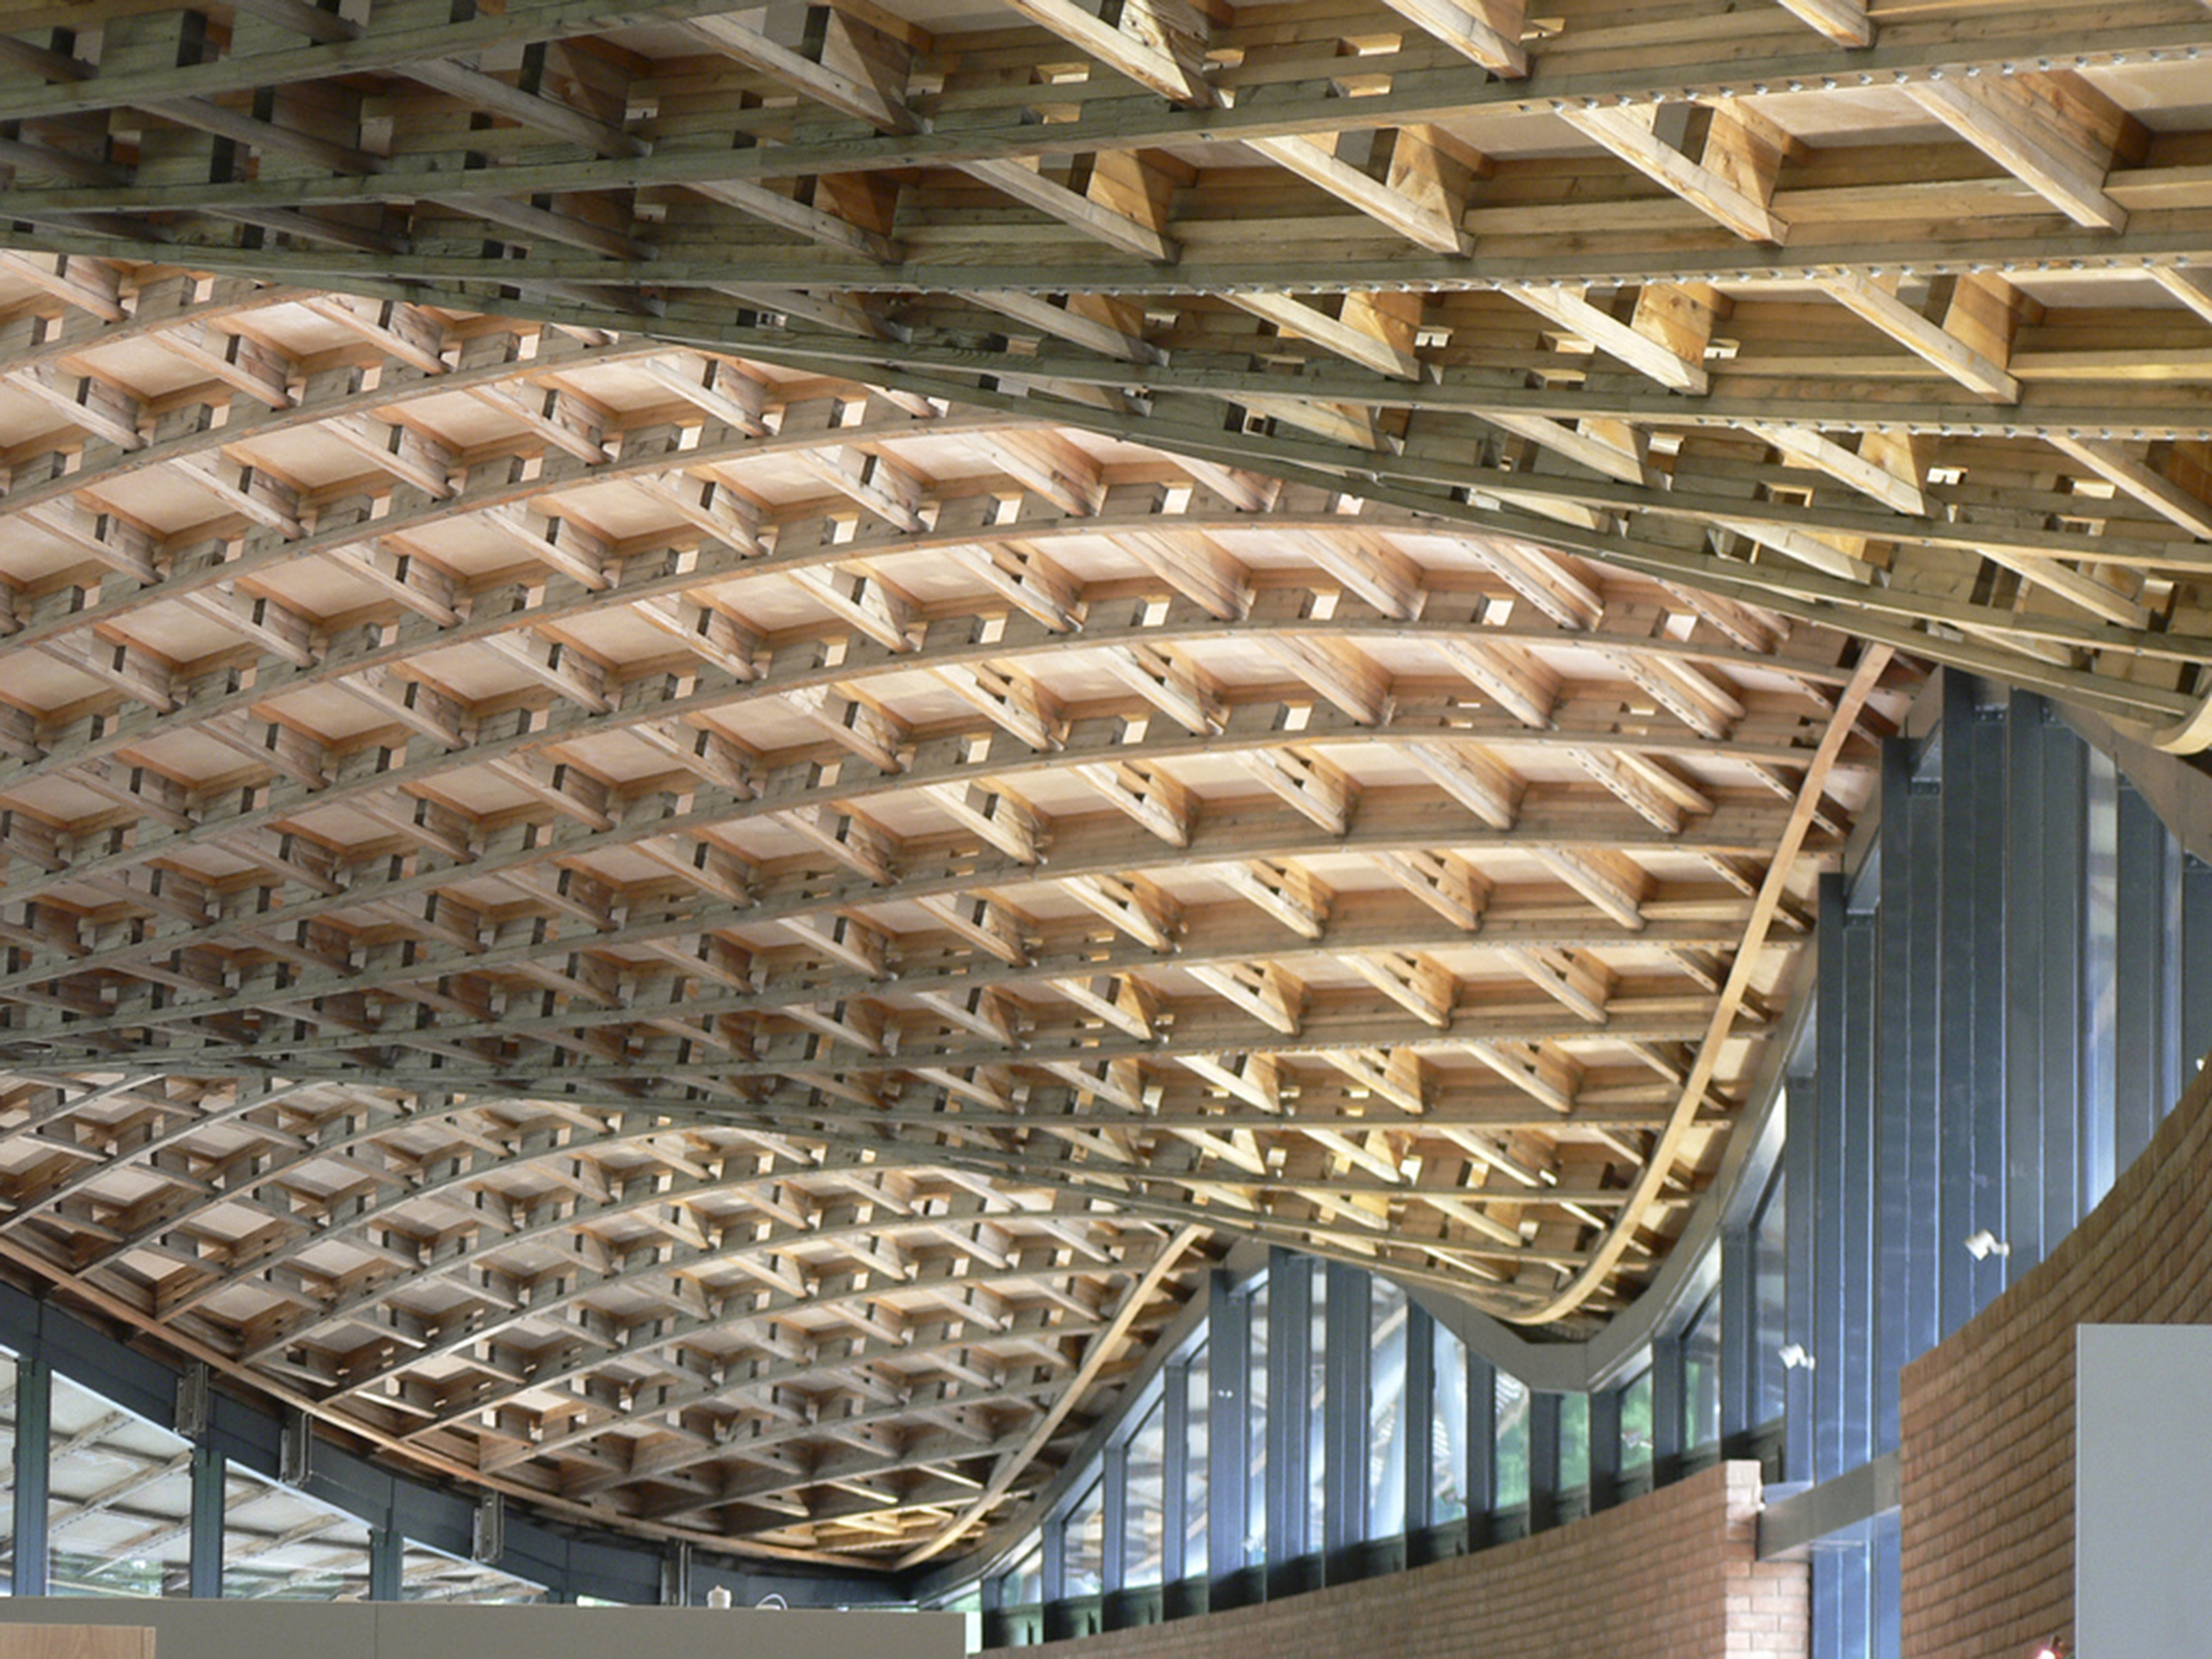
\includegraphics[width=\textwidth]{savill_b.jpg}
		\caption{Interior view}
		\label{fig:savill_a}
	\end{subfigure}%
	\hspace{\MediaGutterWidth}%
	\begin{subfigure}[b]{\TwoMediaWidth}
		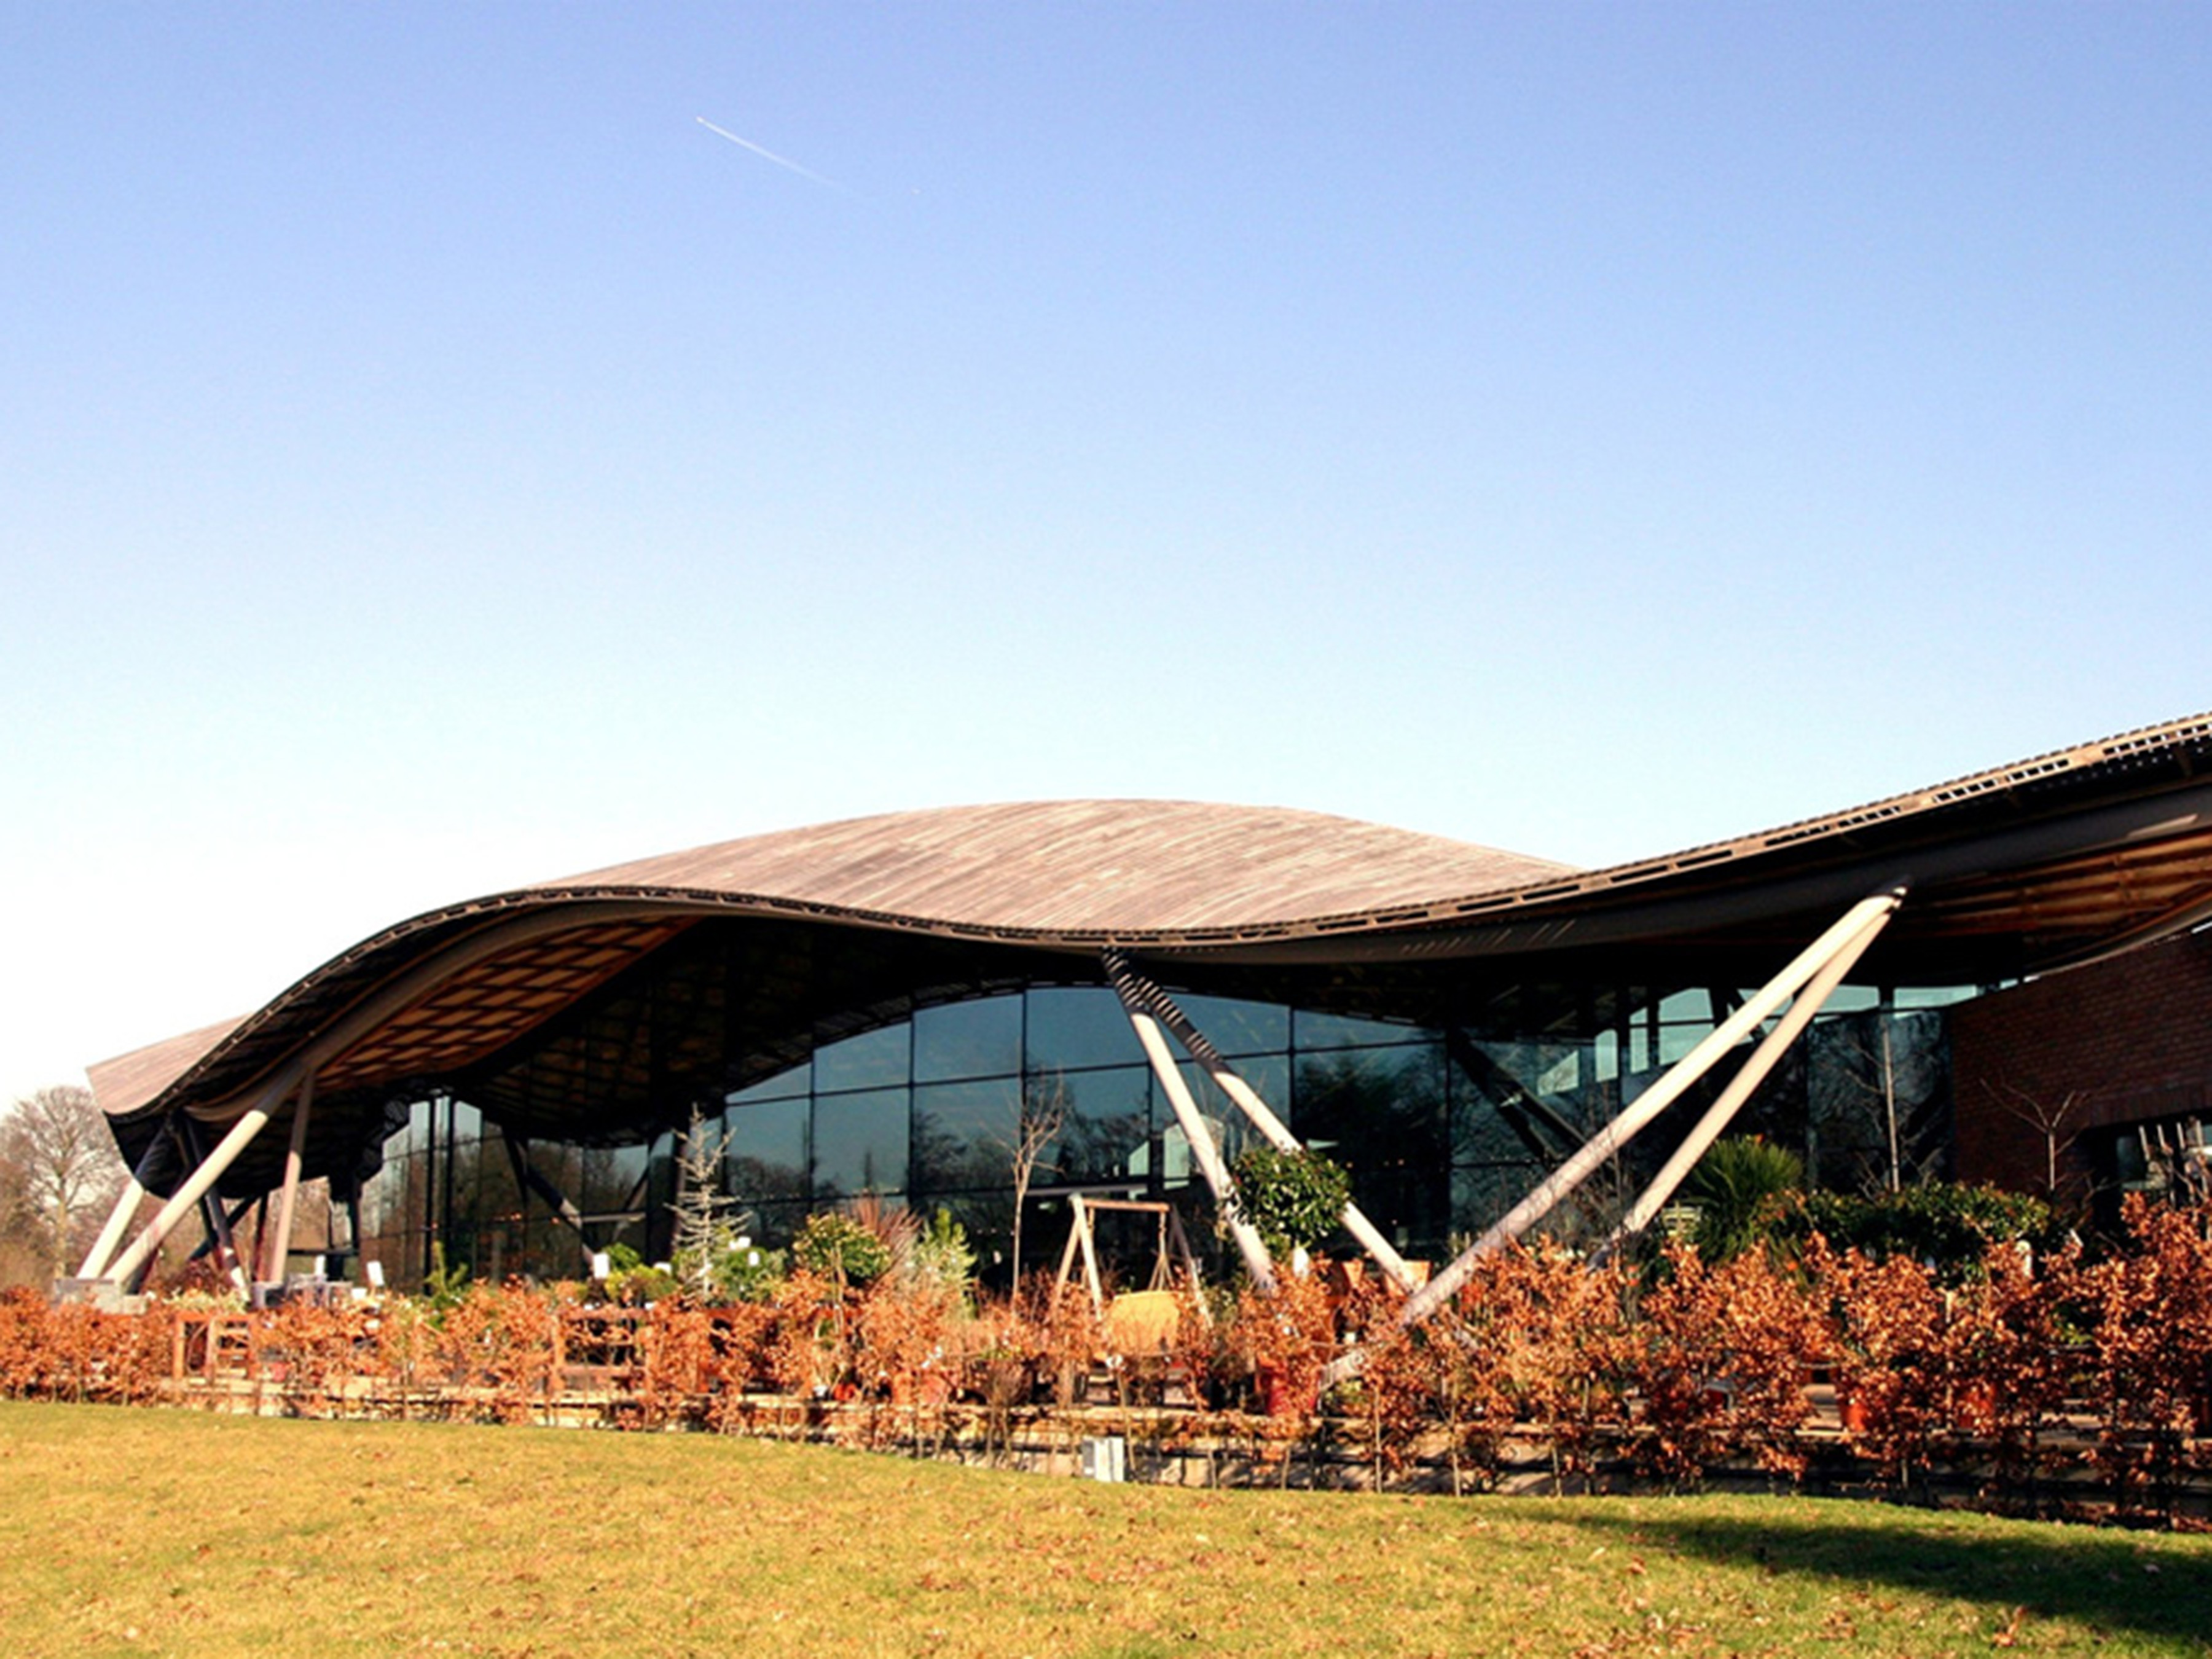
\includegraphics[width=\textwidth]{savill_a.jpg}
		\caption{Exterior view}
		\label{fig:savill_b}
	\end{subfigure}
	\caption[Timber gridshell built in 2006 in Savill, England]{Timber gridshell built in 2006 in Savill, England.}
	\label{fig:savill}
	%
	%
	% \hrule
\end{figure}

\clearpage
\begin{tikzpicture}[remember picture,overlay]
	\node[anchor=north east,inner sep=0pt] at (current page.north east)
	{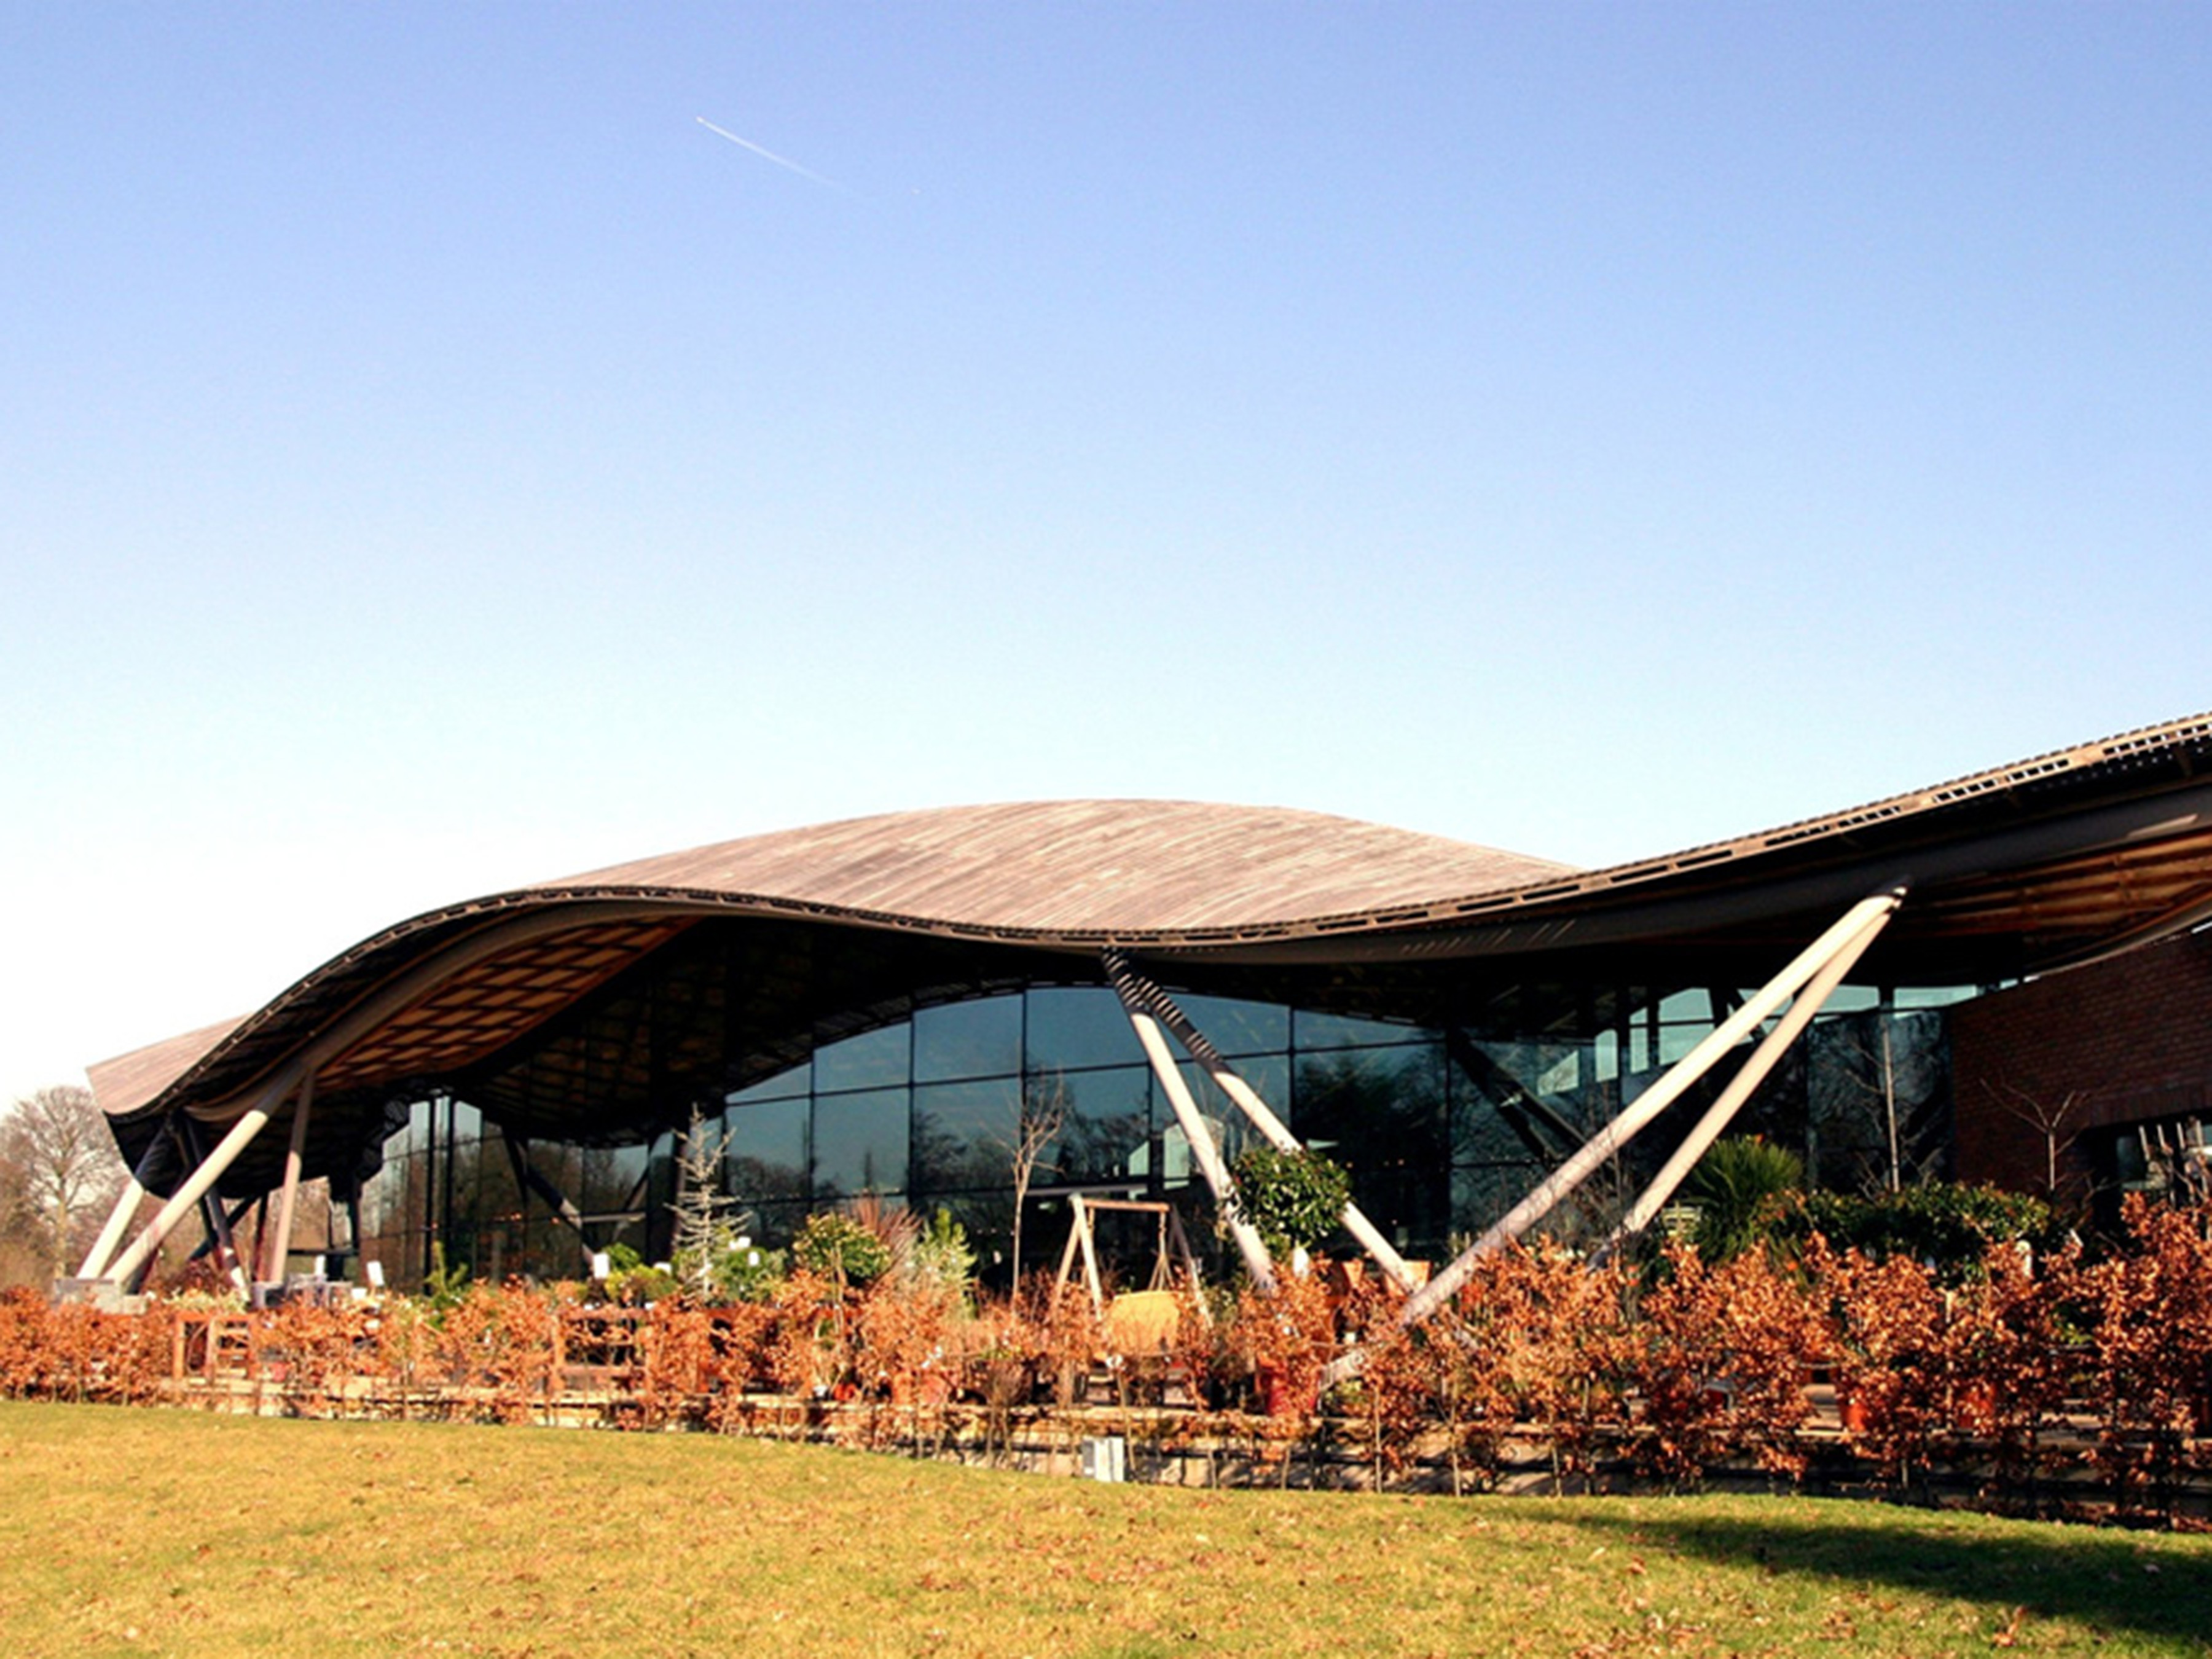
\includegraphics[width=\paperwidth]{savill_a.jpg}};
\end{tikzpicture}

\clearpage
\begin{tikzpicture}[remember picture,overlay]
	\node[anchor=north east,inner sep=0pt] at (current page.north east)
	{
	\begin{minipage}{5cm}
		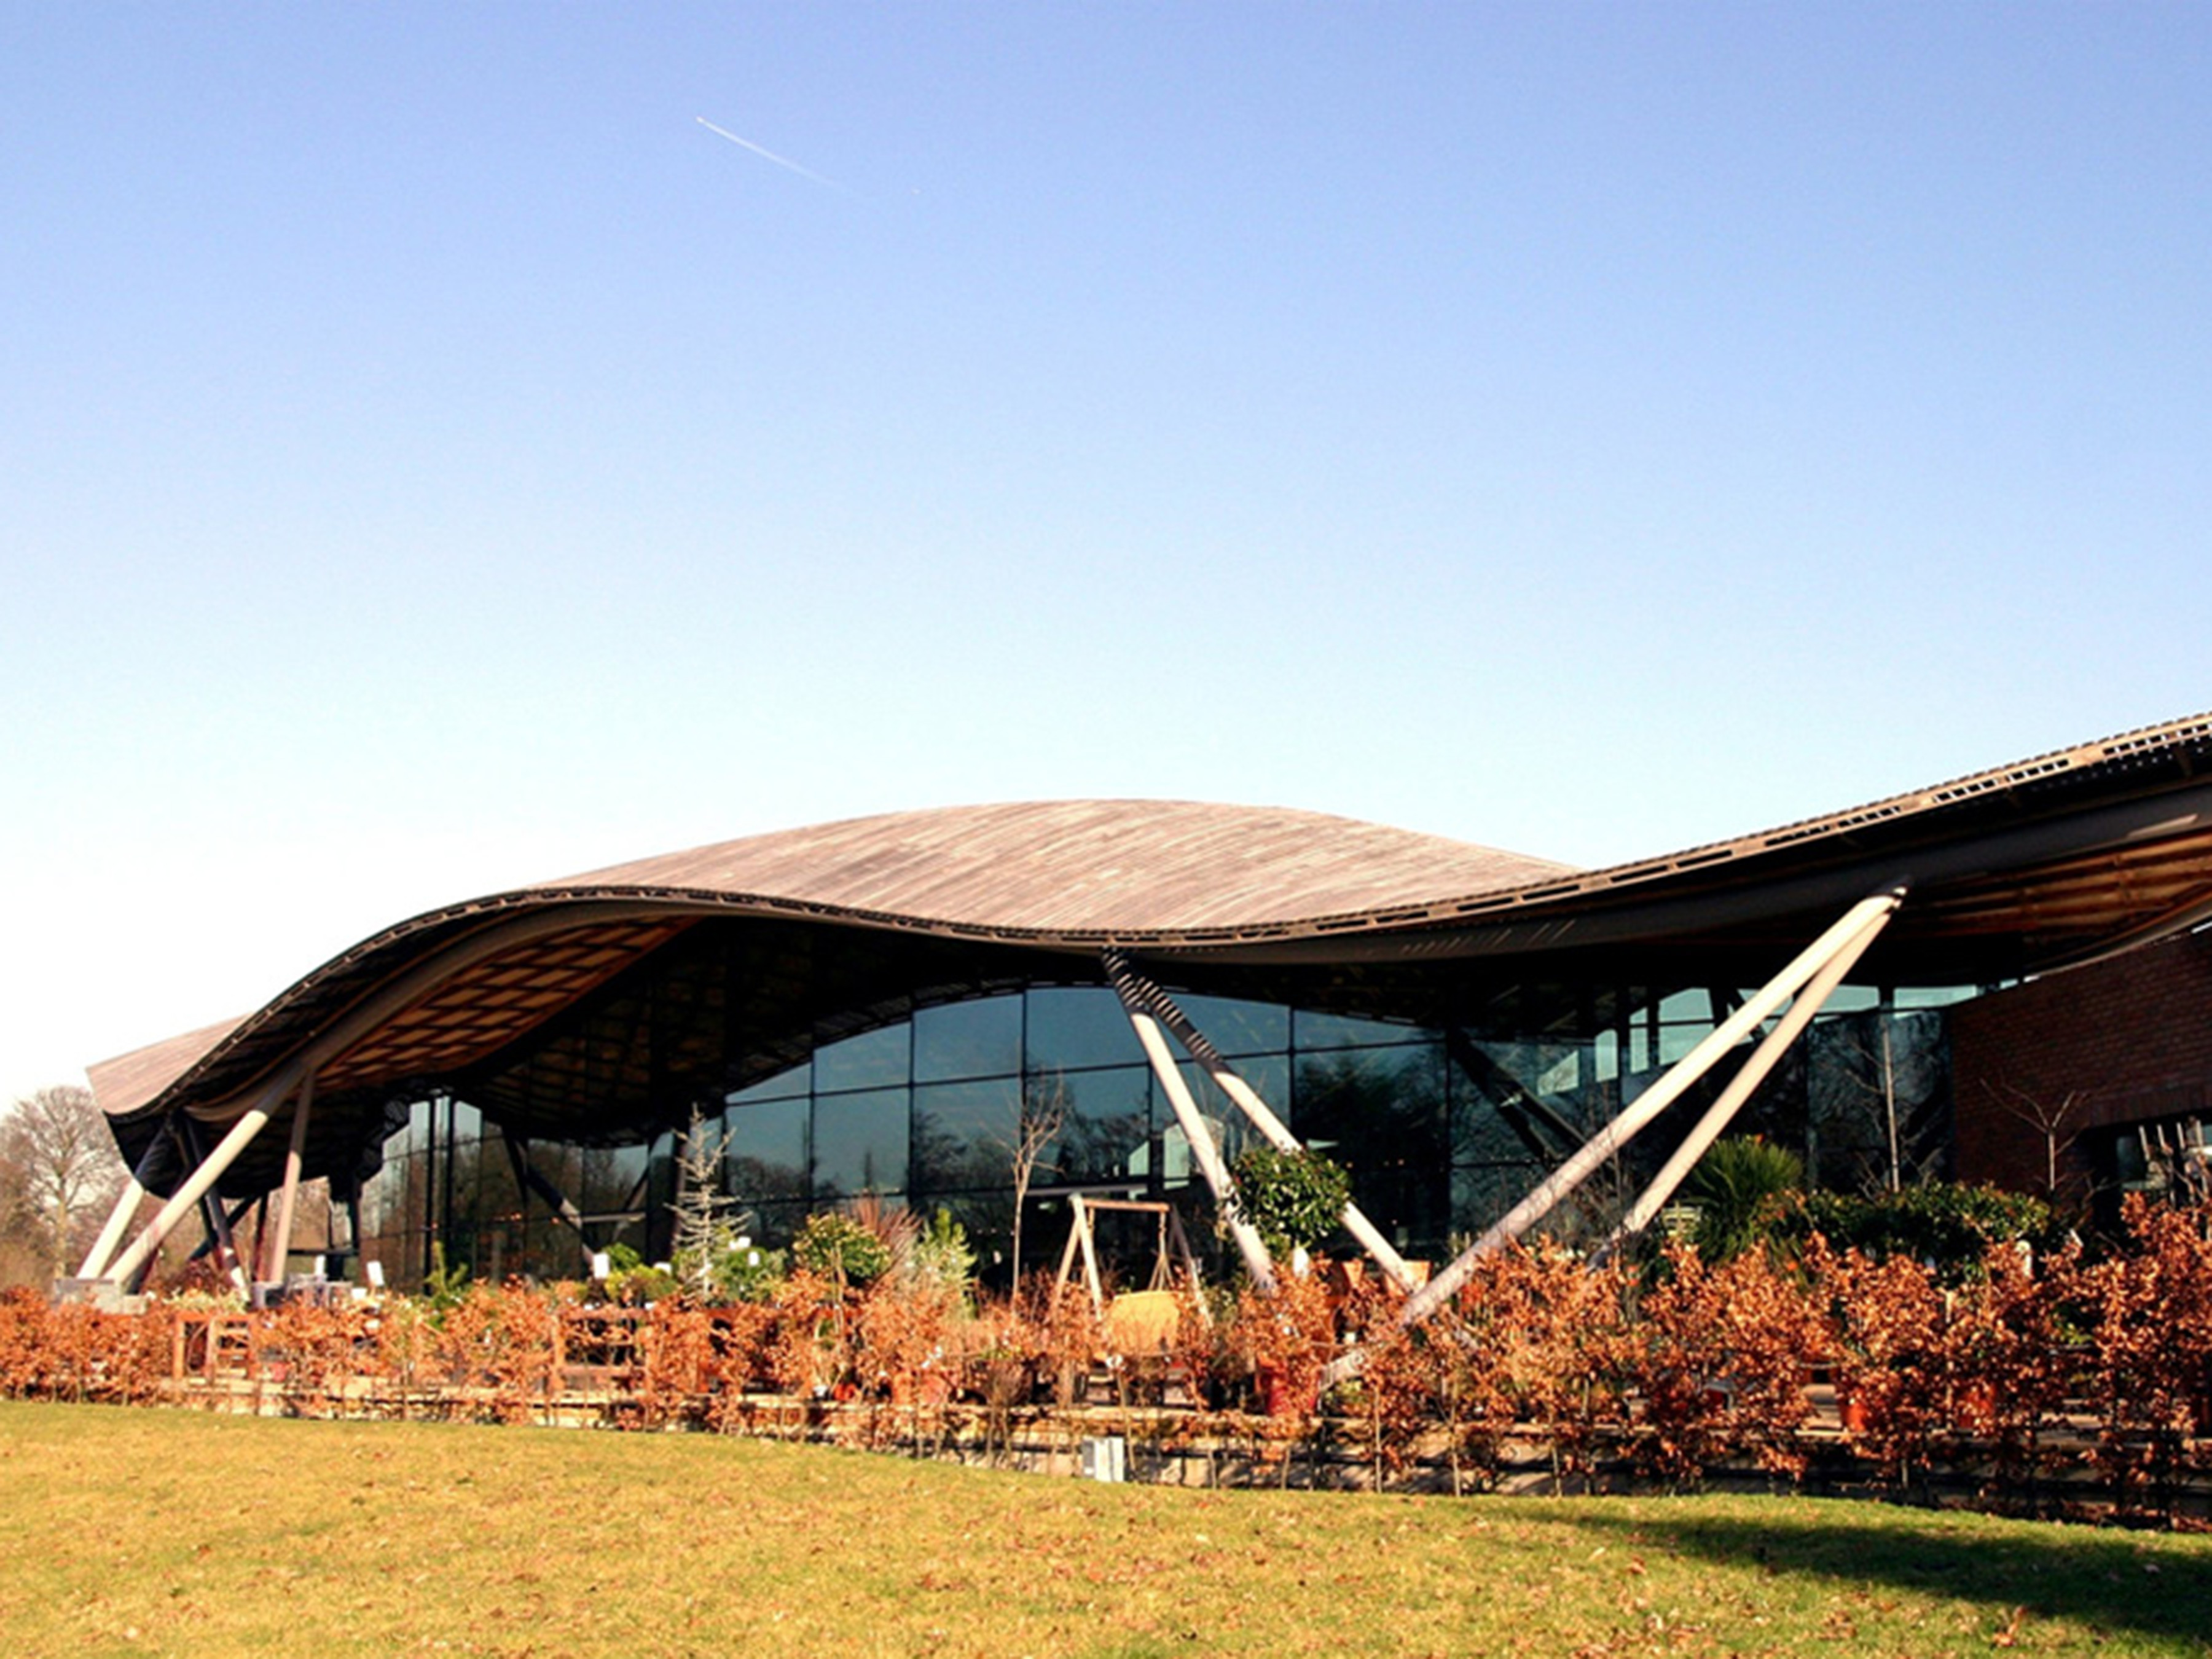
\includegraphics[width=\paperwidth]{savill_a.jpg}
		\captionof{figure}{Some here}
	\end{minipage}
	};
\end{tikzpicture}

\clearpage
\begin{tikzpicture}[remember picture,overlay]
	\node[anchor=north west,inner sep=0pt] at (current page.north west)
	{
	\begin{minipage}{\textwidth}
		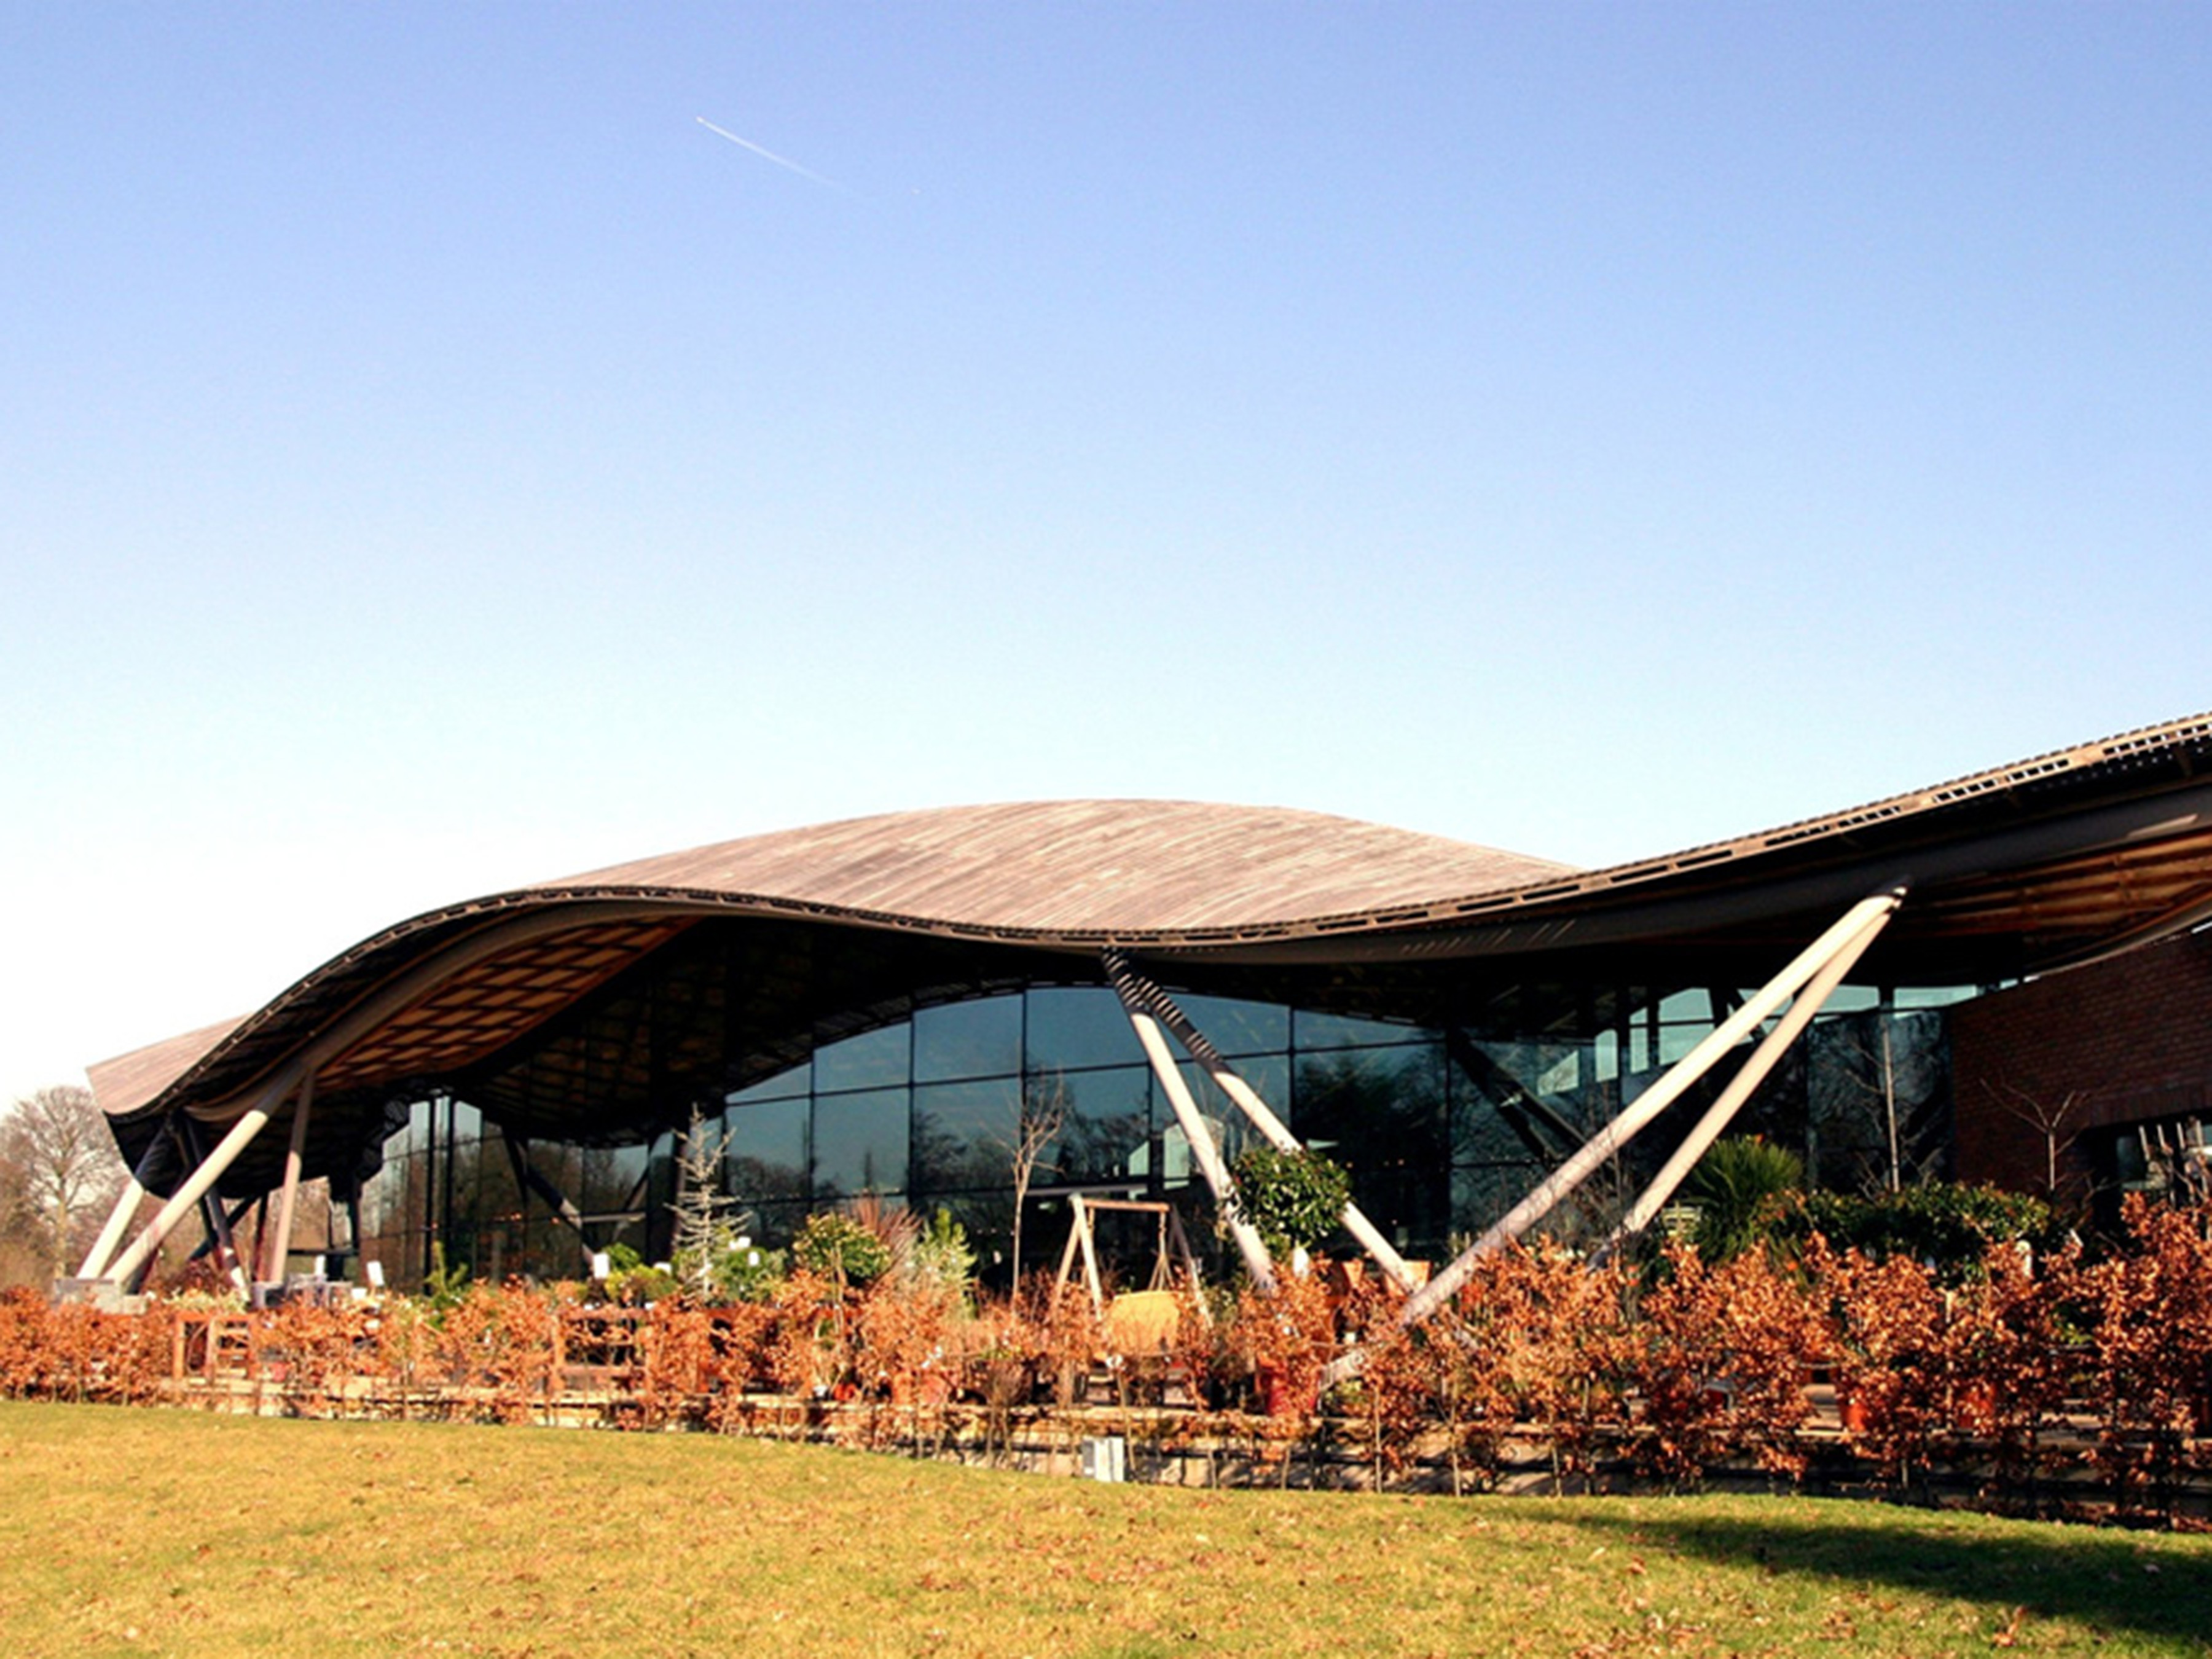
\includegraphics[width=\textwidth]{savill_a.jpg}
		\captionof{subfigure}{}{\label{fig:savill_d}}
	\end{minipage}
	};
\end{tikzpicture}

REF : \cref{fig:savill_d}


% \setlength{\unitlength}{1cm}
% % \begin{picture}(50,50)
% % 	\put(0,0){\hbox{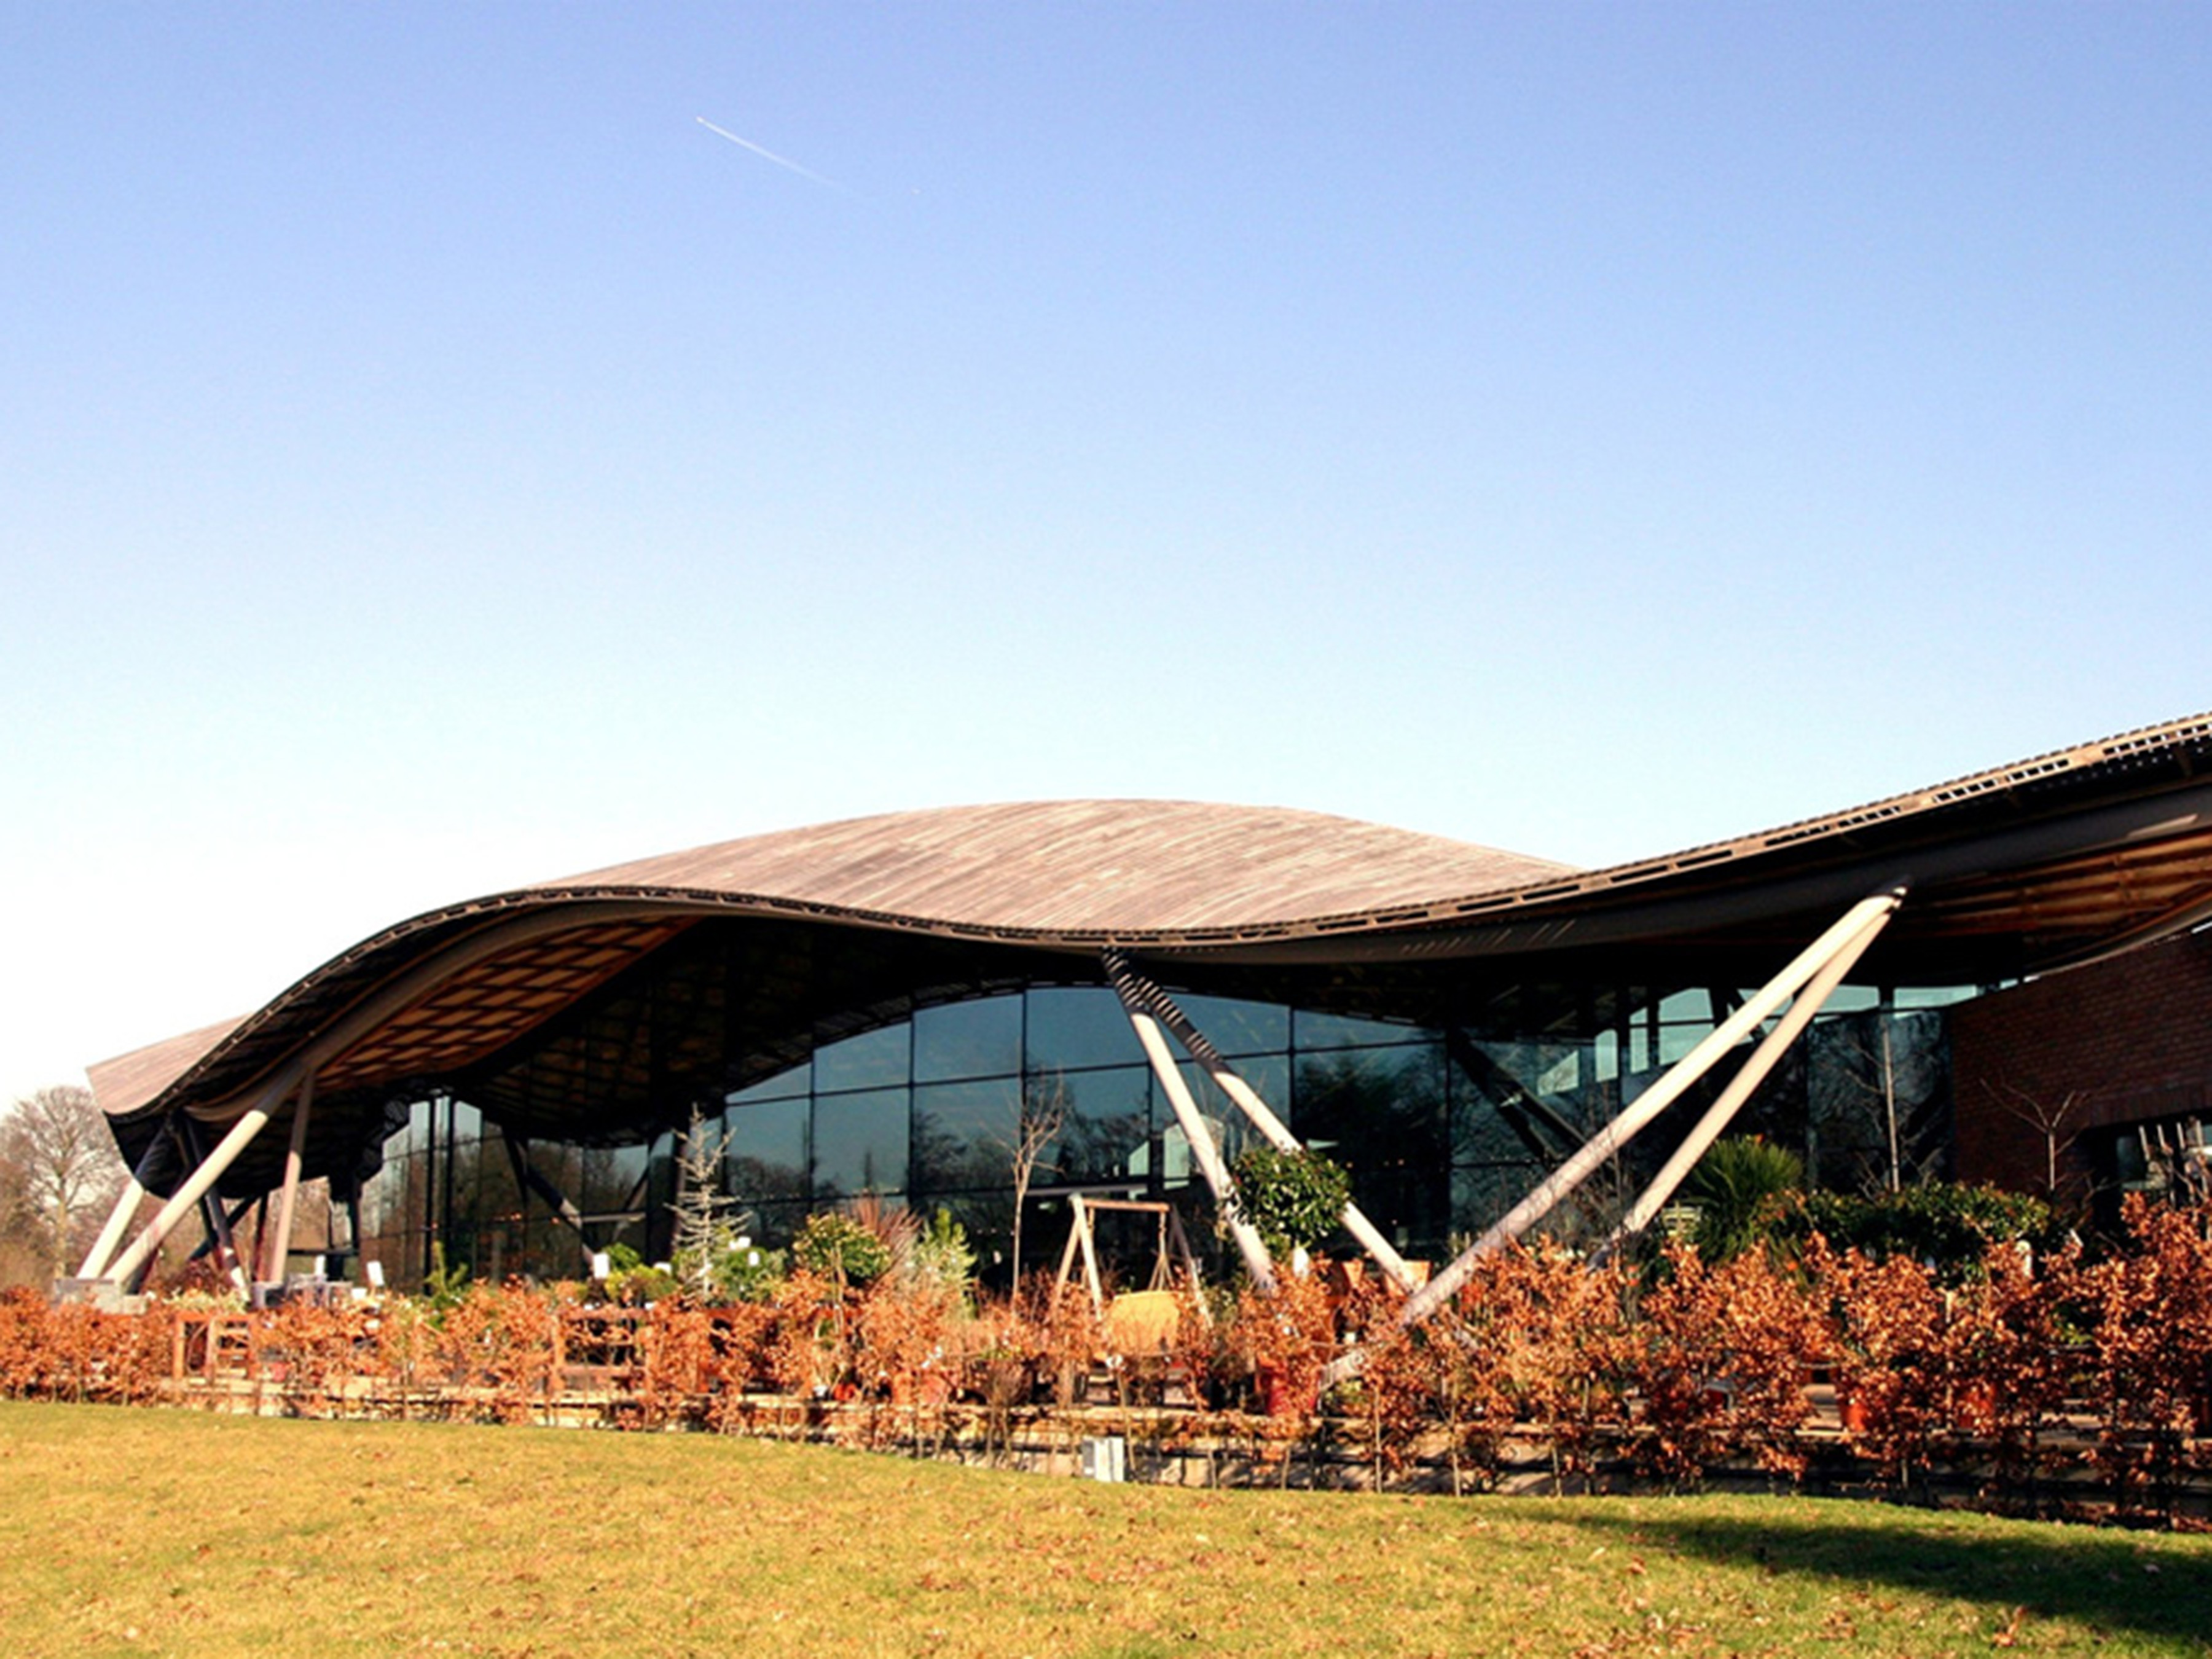
\includegraphics[width=\paperwidth]{savill_a.jpg}}}
% % \end{picture}

% \begin{picture}(0,-10)
% \put(0,0){%
% \begin{minipage}{0.48\linewidth}
% 	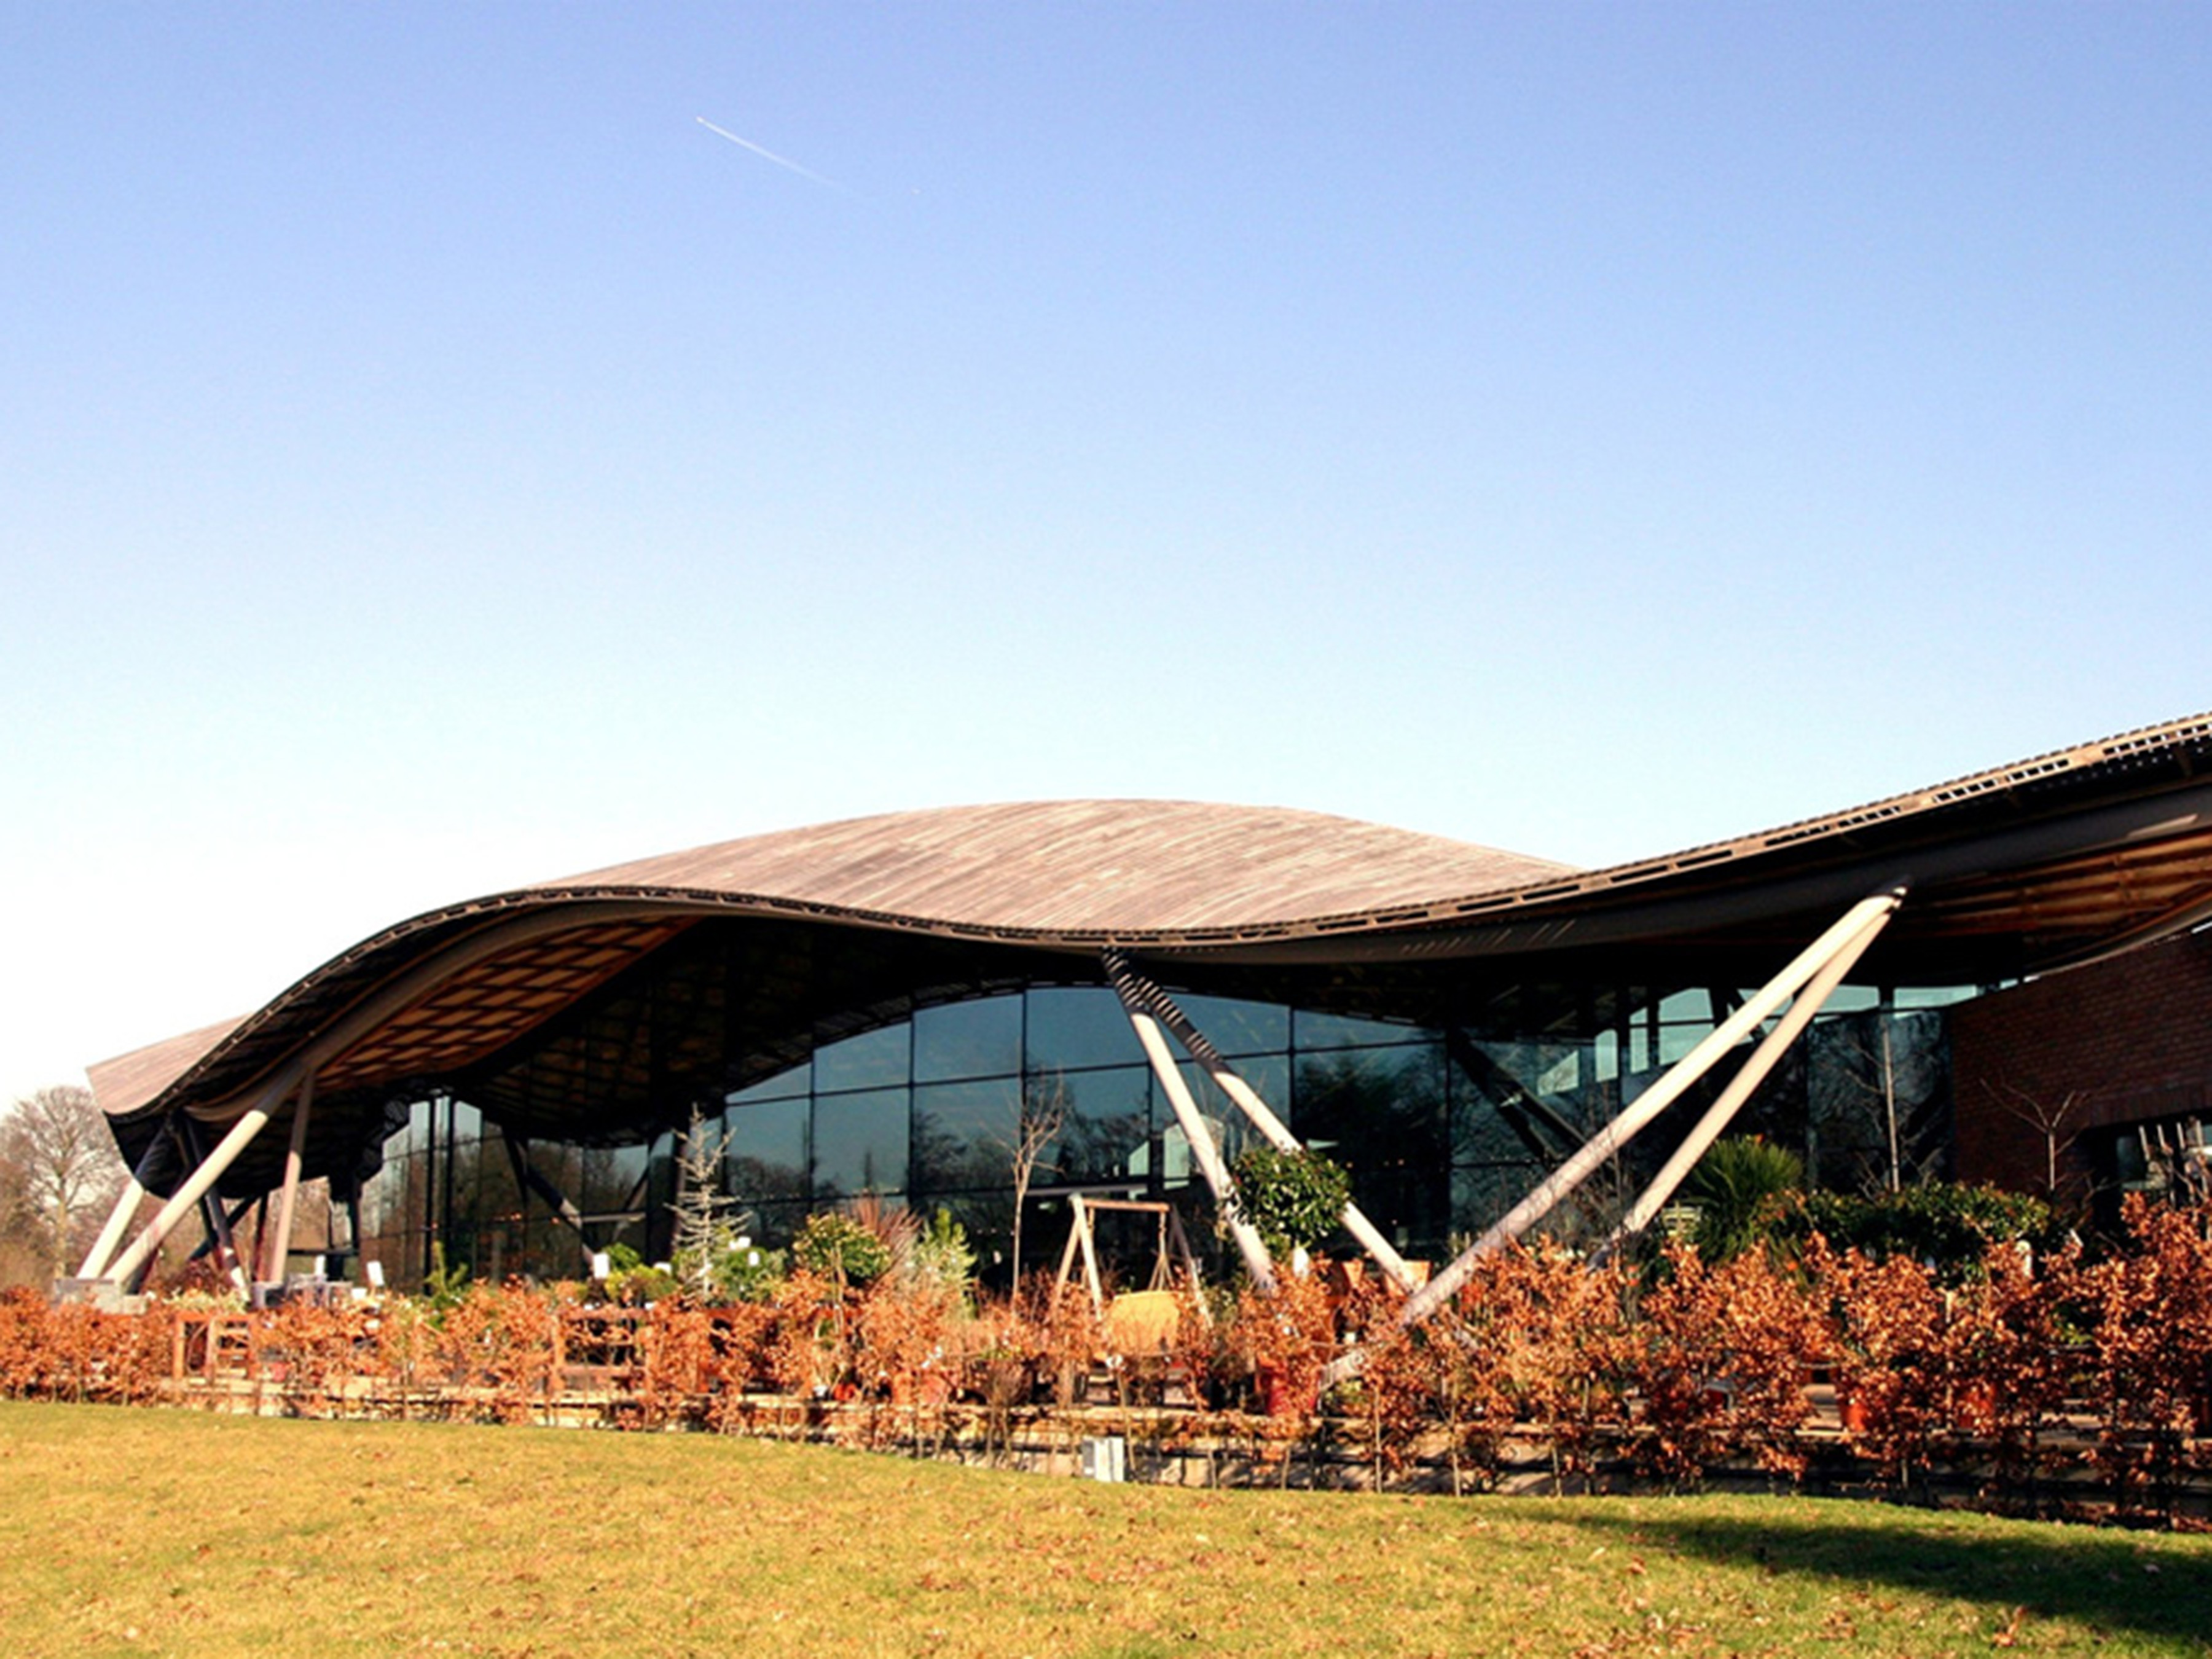
\includegraphics[width=\linewidth]{savill_a.jpg}
% 	\captionof{figure}{Some here}
% \end{minipage}%
% }
% \end{picture}

%  \begin{textblock}{2.5}(\GetX{2cm},\GetY{0cm})
% 	\raggedright
% 	Work is of two kinds: first, altering
% 	the position of matter at or near the
% 	earth’s surface relatively to other such
% 	matter; second, telling other people
% 	to do so.
% \end{textblock}

\begin{textblock*}{10cm}[0,0](0cm,0cm)
	\raggedright
	Work is of two kinds: first, altering
	the position of matter at or near the
	earth’s surface relatively to other such
	matter; second, telling other people
	to do so.
\end{textblock*}

% \begin{textblock}{2.5}[1,1](1,1)
% 	\raggedright
% 	Work is of two kinds: first, altering
% 	the position of matter at or near the
% 	earth’s surface relatively to other such
% 	matter; second, telling other people
% 	to do so.
% \end{textblock}



%
%\begin{figure}[p]
%     	\centering
%%	\begin{fullpage}
%		\subfloat[][Interior view]{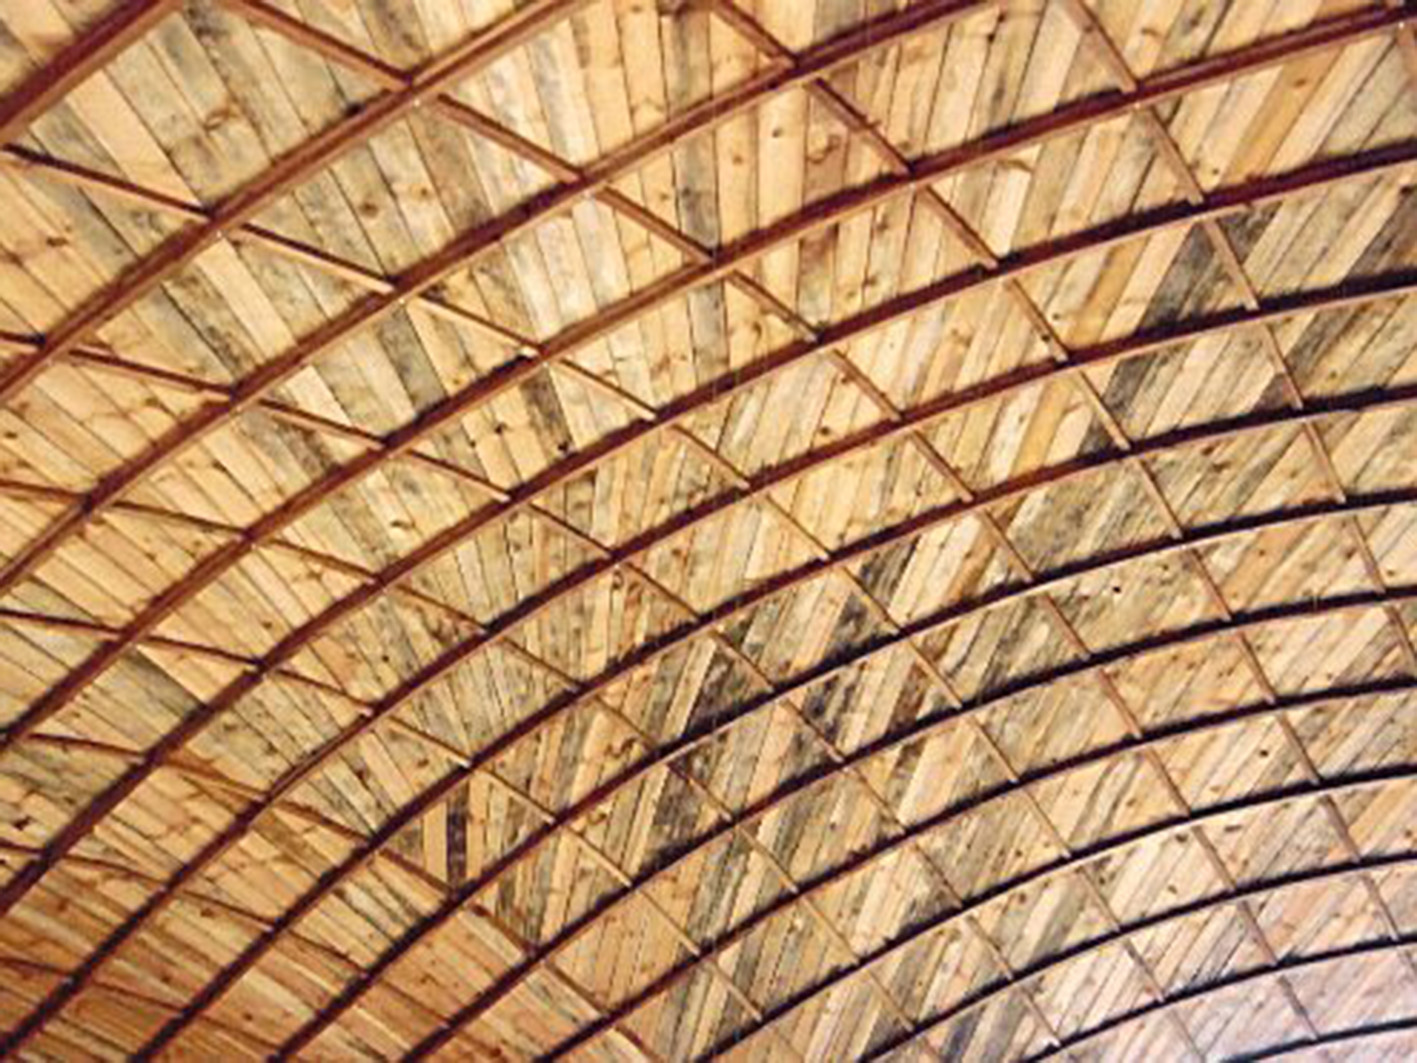
\includegraphics[width=\TwoMediaWidth]{pishwanton_int.jpg}\label{fig:pishwanton_a}}
%		\hspace{\MediaGutterWidth}% (%) required to prevent extra space
%		\subfloat[][Exterior view]{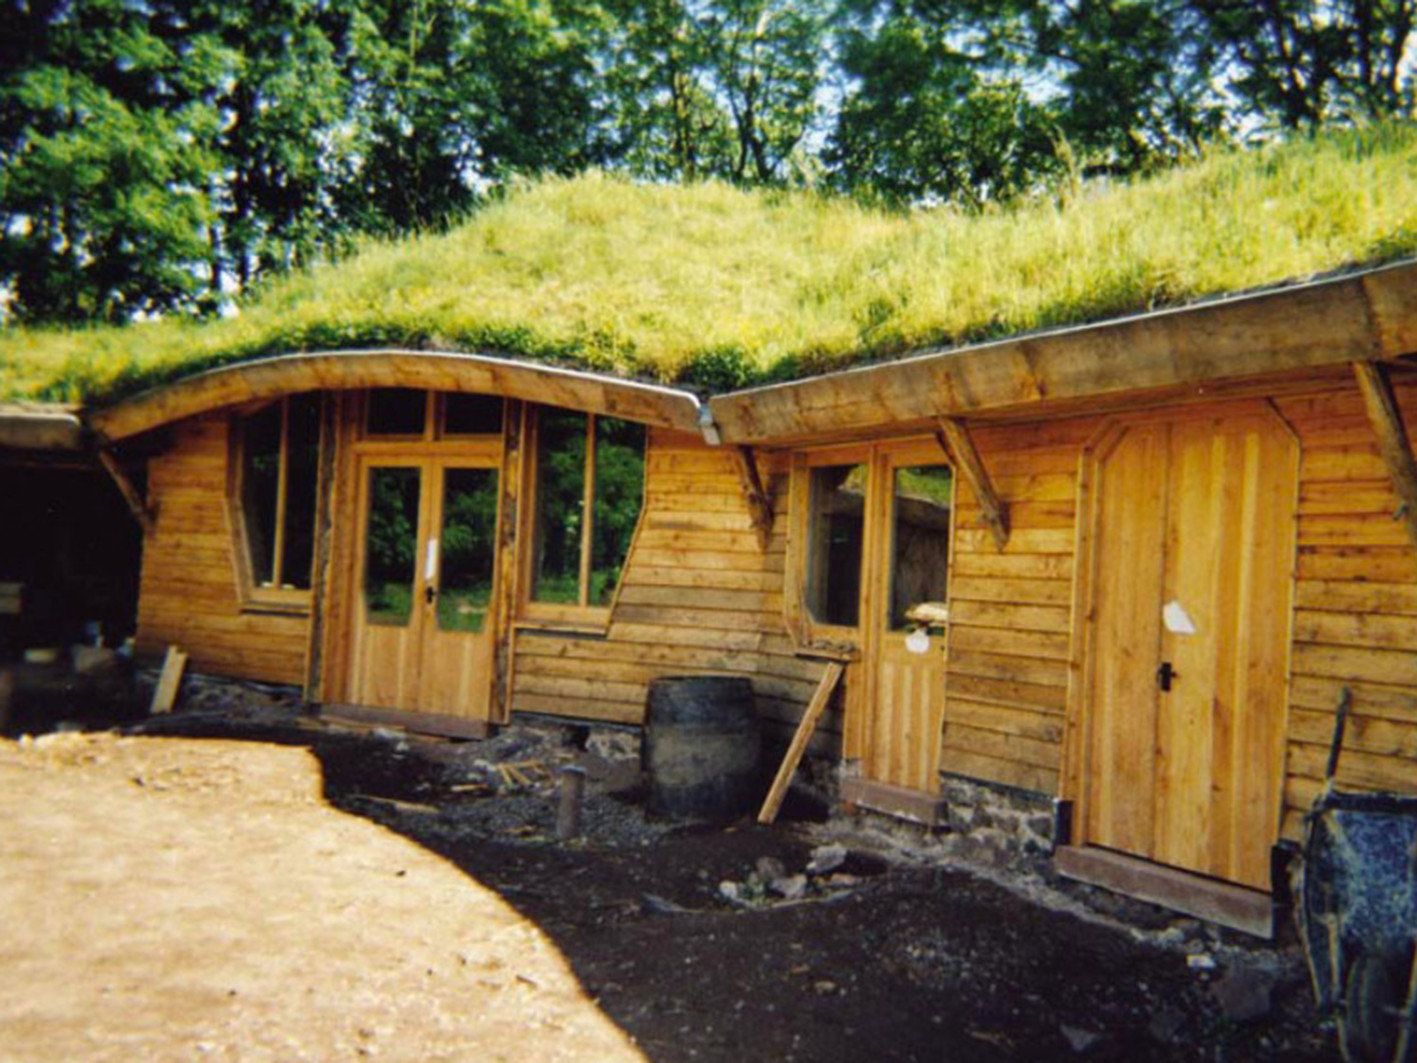
\includegraphics[width=\TwoMediaWidth]{pishwanton_ext.jpg}\label{fig:pishwanton_b}}
%%		\vspace{10pt}
%		\captionof{figure}[Timber gridshell built in 2002 in Pishwanton, England]{Timber gridshell built in 2002 in Pishwanton, England.}
%		\label{fig:pishwanton}
%		%
%		\vspace{\fill}
%		%
%		\subfloat[][Interior view]{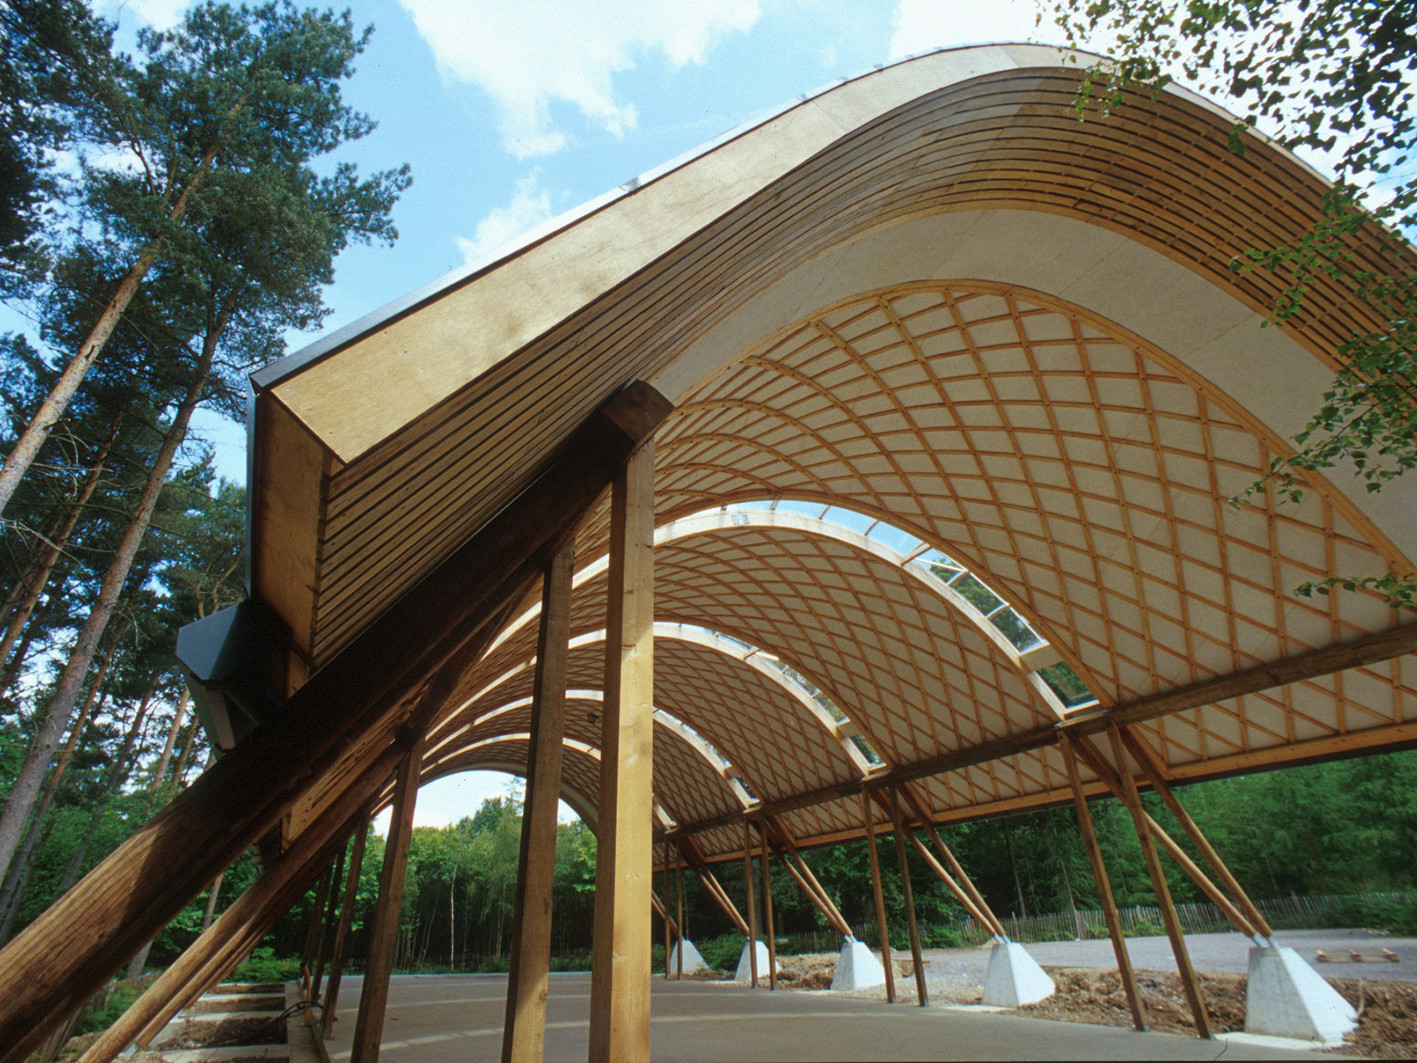
\includegraphics[width=\TwoMediaWidth]{flimwell_int.jpg}\label{fig:flimwell_a}}
%		\hspace{\MediaGutterWidth}% (%) required to prevent extra space
%		\subfloat[][Exterior view]{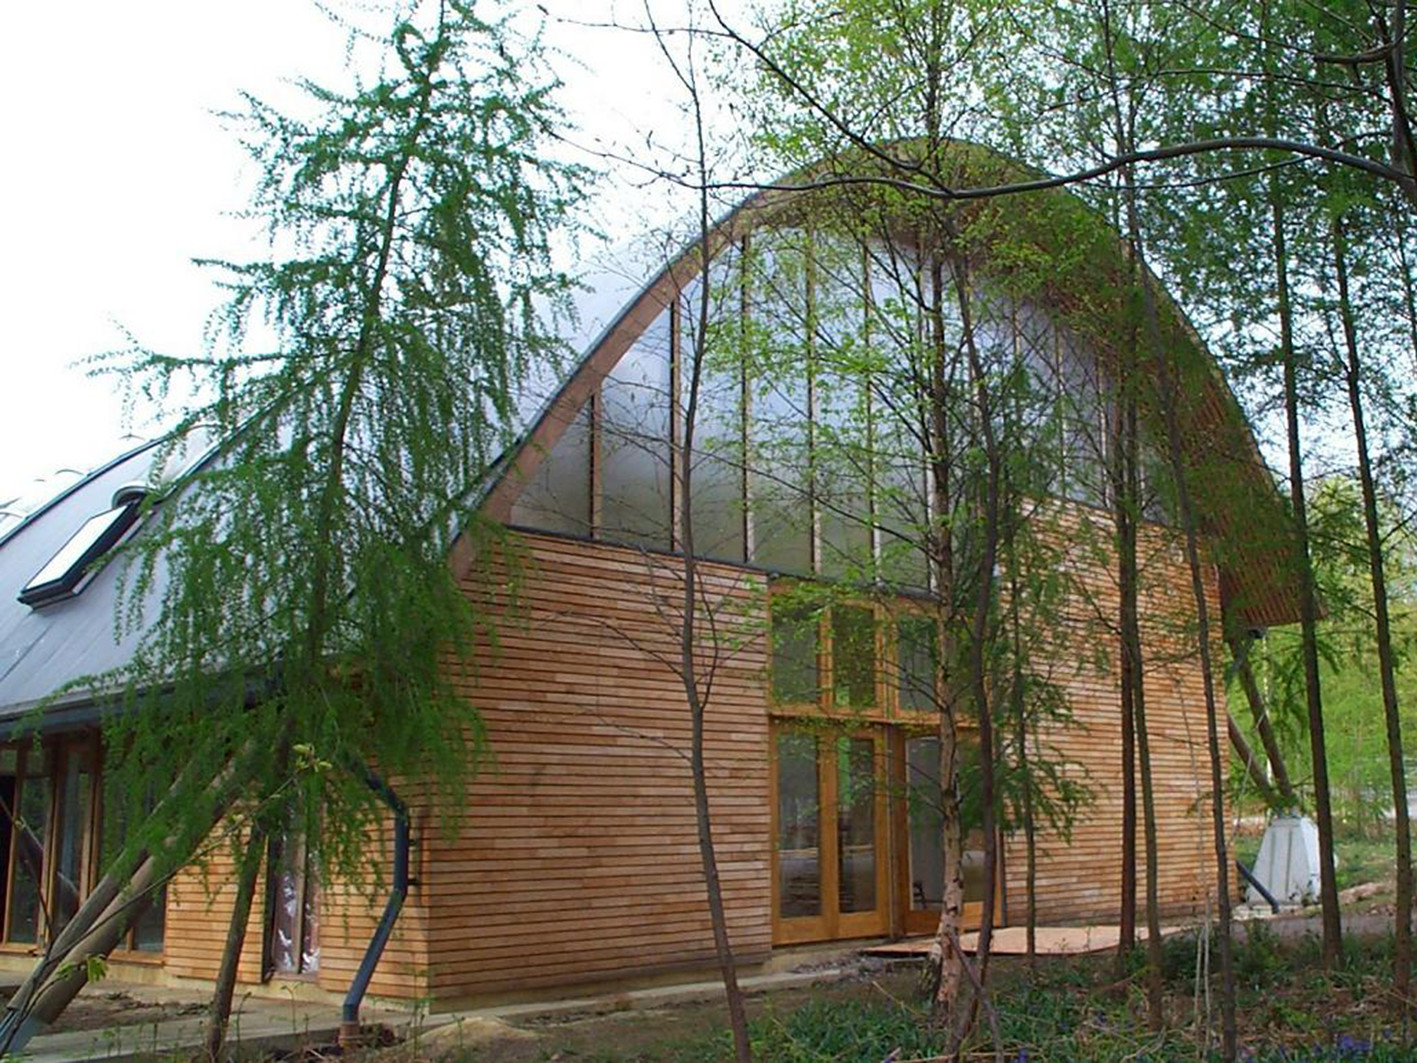
\includegraphics[width=\TwoMediaWidth]{flimwell_ext.jpg}\label{fig:flimwell_b}}
%%		\vspace{10pt}
%		\captionof{figure}[Timber gridshell built in 2003 in Filmwell, England]{Timber gridshell built in 2003 in Filmwell, England.}
%		\label{fig:flimwell}
%		%
%		\vspace{\fill}
%		%
%		\subfloat[][Interior view]{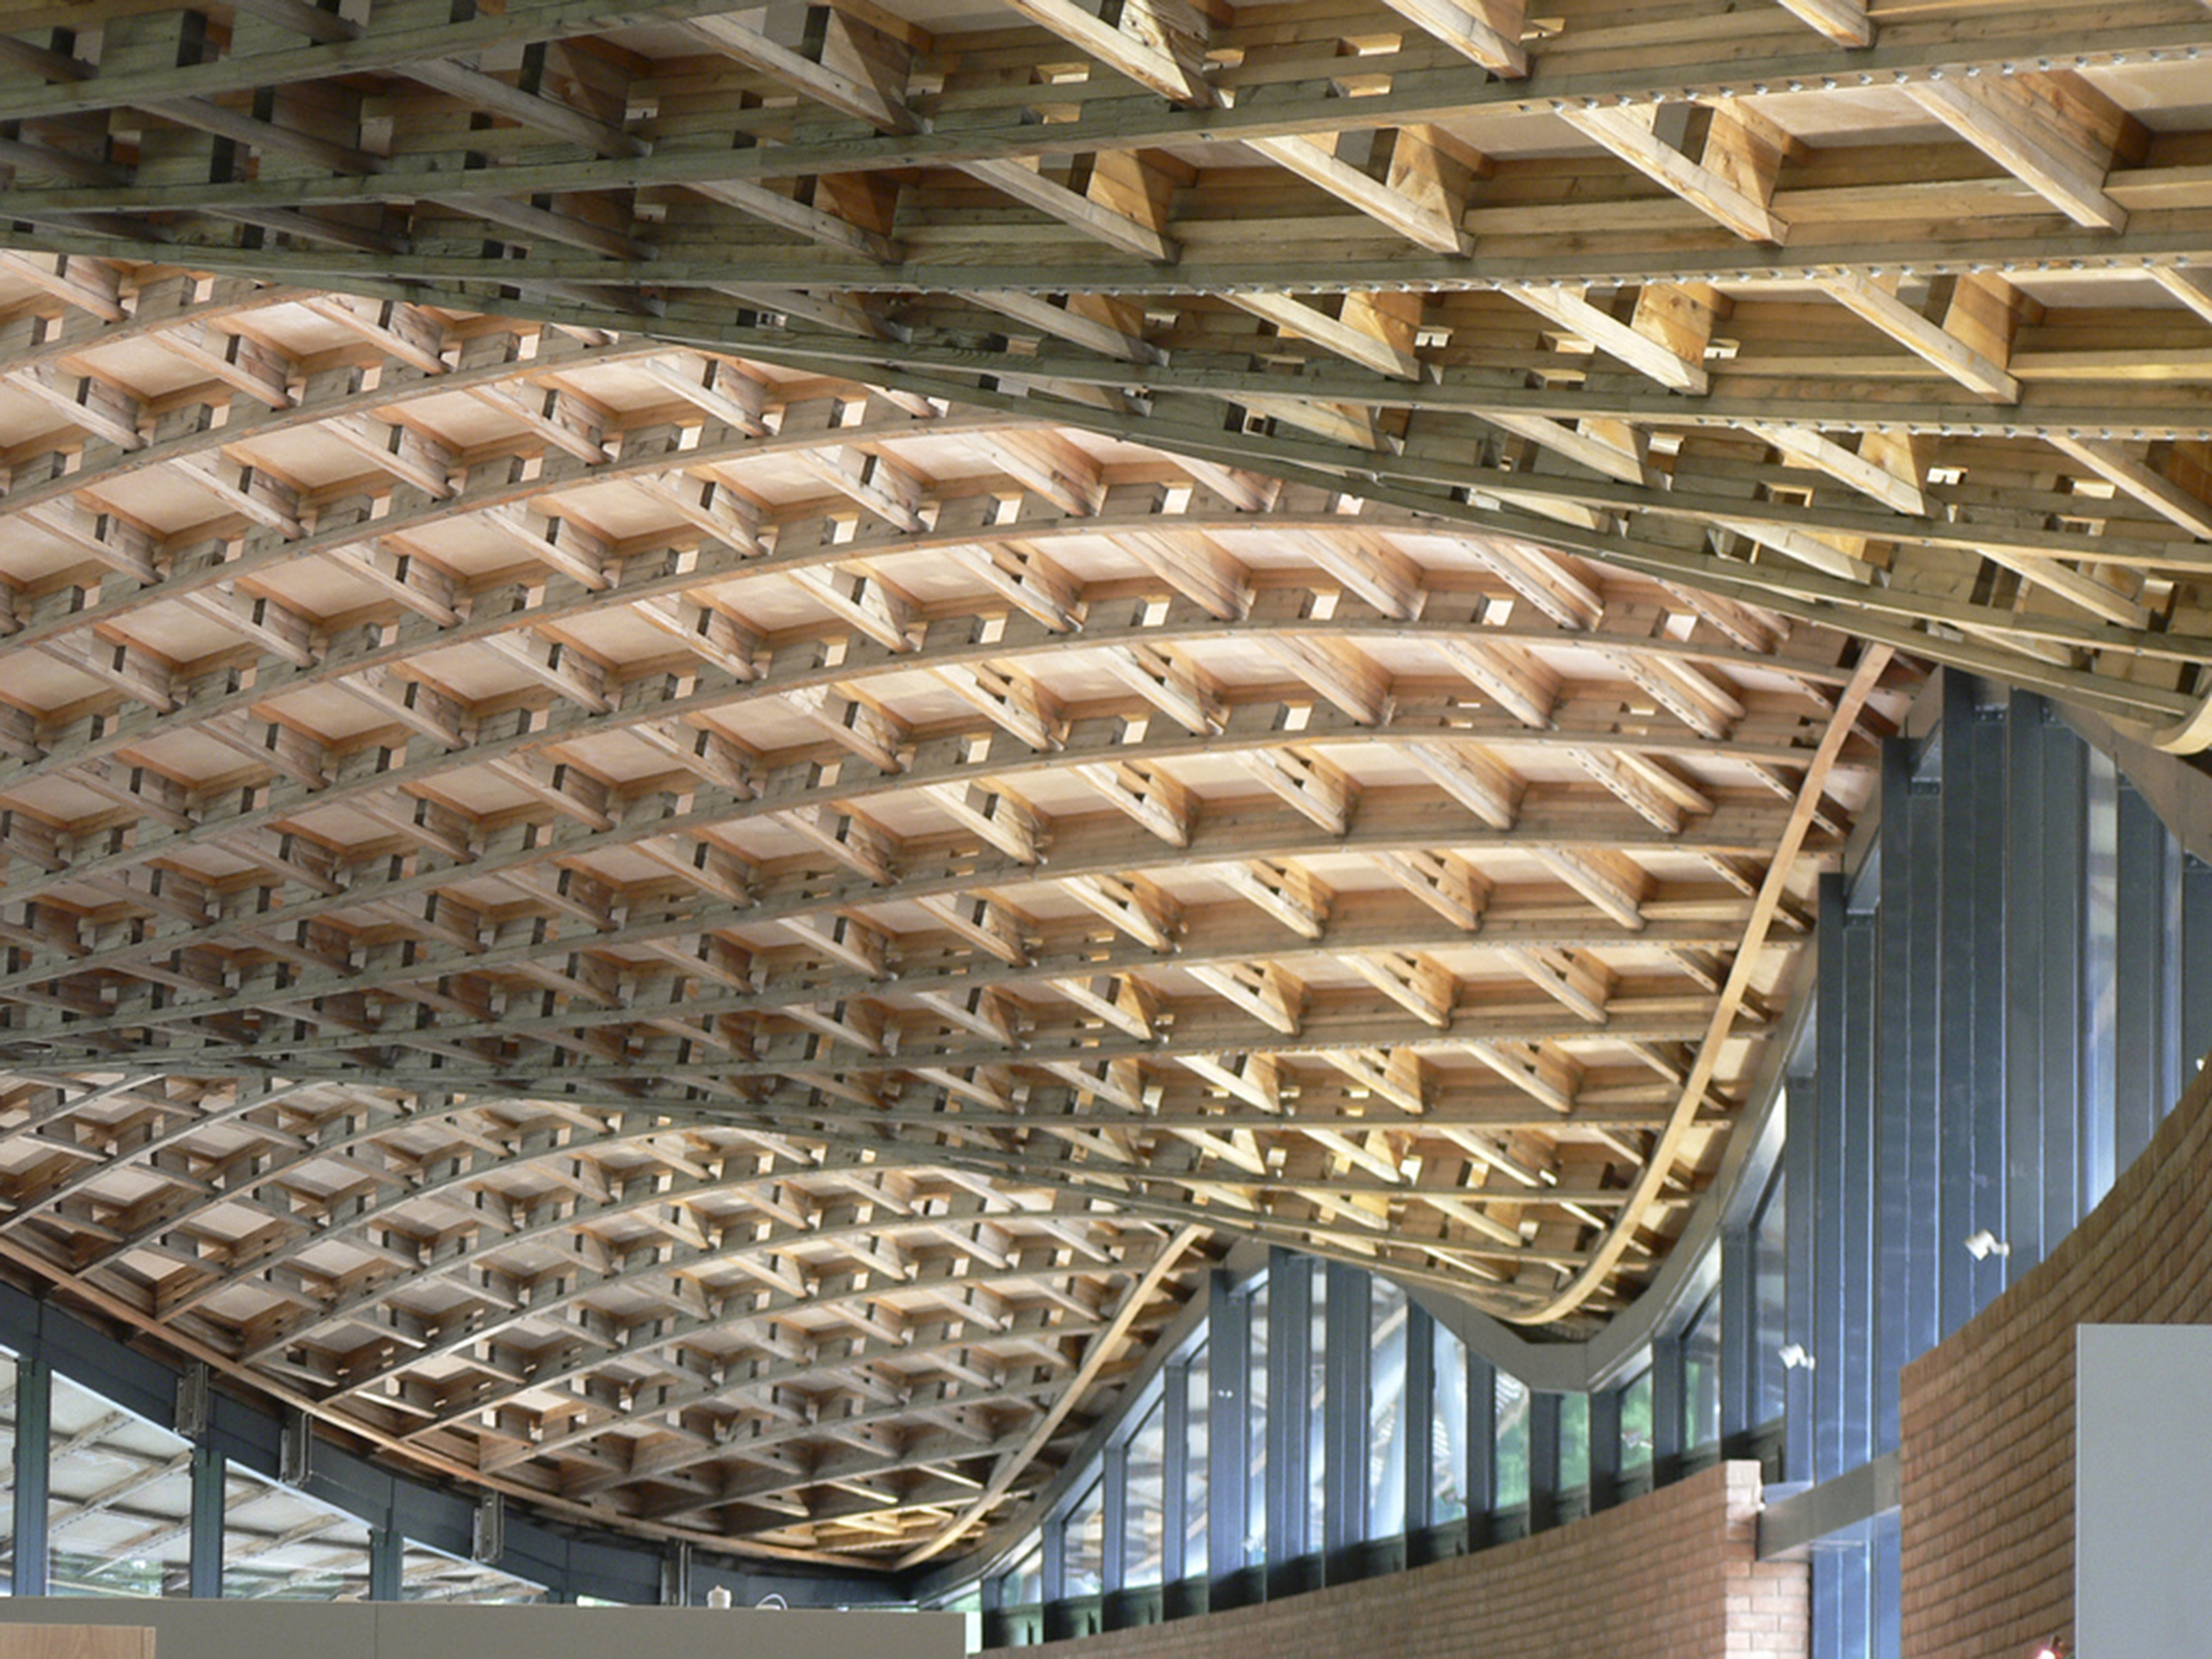
\includegraphics[width=\TwoMediaWidth]{savill_b.jpg}\label{fig:savill_a}}
%		\hspace{\MediaGutterWidth}% (%) required to prevent extra space
%		\subfloat[][Exterior view]{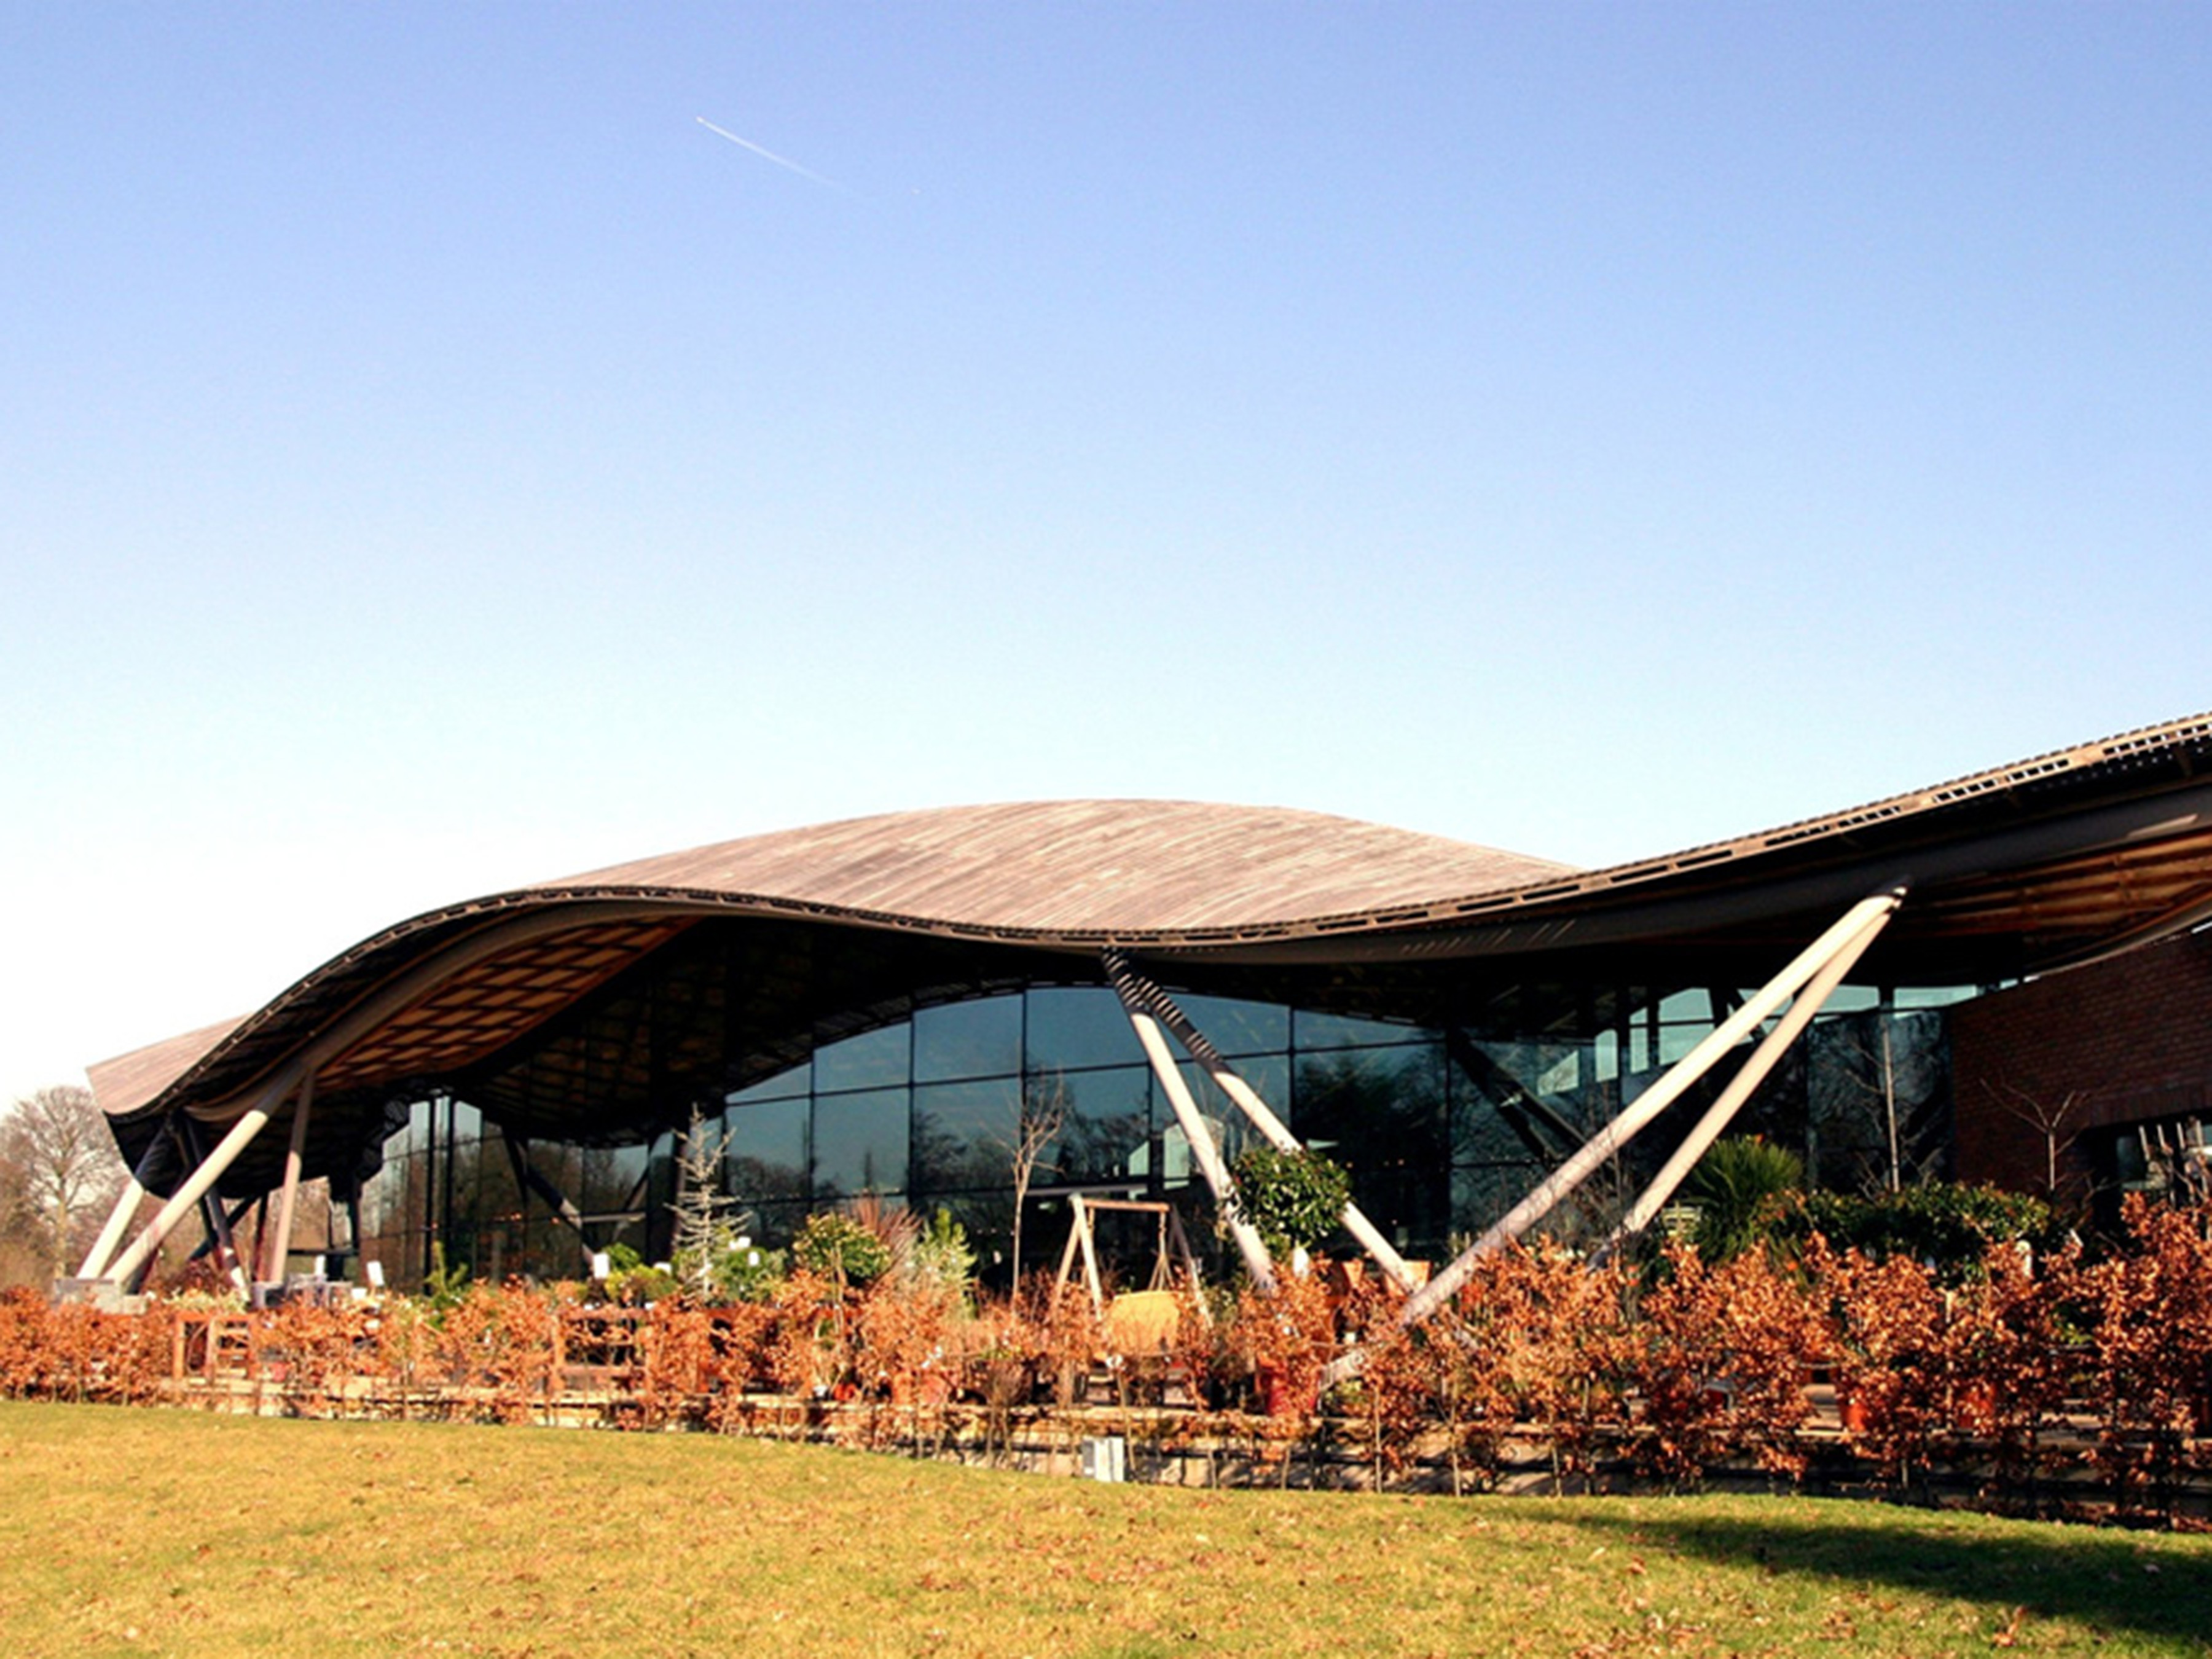
\includegraphics[width=\TwoMediaWidth]{savill_a.jpg}\label{fig:savill_b}}
%%		\vspace{10pt}
%		\captionof{figure}[Timber gridshell built in 2006 in Savill, England]{Timber gridshell built in 2006 in Savill, England.}
%		\label{fig:savill}
%%	\end{fullpage}
%\end{figure}
%%
\printbibliography[segment=\therefsegment,heading=subbibliography]

	% \part{Fake}
	% \part{Fake}
	% \part{Fake}

	% \part{This is a very long part title}
	% \chapter{With a very veru very very lonnnnnnngg premier chapitre Linel}
	% \section{Une section}
	% \kant[1-10]

	
	% \chapter{Mon premier chapitre Linel}
	% \section{Une section}
	% \kant[1-10]
	
	% \subsection{Une section}
	% \kant[1-10]
	% \subsection{Une section}
	% \kant[1-10]
	% \subsection{Une section}
	% \kant[1-10]

	% \section{Une section}
	% \kant[1-10]
	% \subsection{Une section}
	% \kant[1-10]
	% \subsection{Une section}
	% \kant[1-10]
	% \subsection{Une section}
	% \kant[1-10]

	% \part{Fake}
	% \chapter{Mon premier chapitre Linel}
	% \section{Une section}
	% \kant[1-10]
	% \section{Une deuxième section}
	% \kant[1-2]
	% \section{Une troisième section}
	% \kant[1-2]
	% \chapter{Mon premier chapitre Linel}
	% \section{Une section}
	% \kant[1-10]
	% \section{Une deuxième section}
	% \kant[1-2]
	% \section{Une troisième section}
	% \kant[1-2]
	% \chapter{Mon premier chapitre Linel}
	% \section{Une section}
	% \kant[1-10]
	% \section{Une deuxième section}
	% \kant[1-2]
	% \section{Une troisième section}
	% \kant[1-2]



	% % Author :  Lionel du Peloux
% Contact : lionel.dupeloux@gmail
% Year : 2017
% !TEX encoding = UTF-8 Unicode

\chapter{Geometry of smooth and discrete space curves}\label{chp:curve}
\section{Introduction}
In this chapter, our goal is to develop a comprehensive view of the geometry of space curves and how to frame such curves. Indeed, framed curve representations are of central importance when dealing with slender beam models, as they are often modeled using curvilinear coordinate systems. This is the kind of representation on which our beam model will be based on.

Although the theoretical beam model takes place in the smooth world, our model will be implemented in a numerical solver, hence the necessity of a discrete representation. However, the two world are intimately related to each other and this is why we chose to present them both in this chapter.\footnote{\citef[preface]{LHospital1696}~: \blockquote{Car les courbes n’étant que des polygones d’une infinité de côtés, \& ne différant
entr' elles que par la différence des angles que ces côtés infiniment petits font
entr'eux~; il n’appartient qu’à l’Analyse des infiniment petits de déterminer la
position de ces cotés pour avoir la courbure qu’ils forment \belp{}}.}

A comprehensive understanding of the geometry of discrete curves will enable to build a beam model with reduced degrees of freedom and capable of representing discontinuities in curvature. This last point is of particular interest when modeling real structures with complex boundary conditions and connexions where concentrated moments are transferred (that is jumps in curvature occur).

\subsection{Overview}
We start this chapter by recalling the fundamentals of smooth parametric curves (see \cref{sec:paramcrvs}). We introduce the \emph{Frenet frame}, a crucial tool for the local characterization of space curves (see \cref{sec:frenet_trihedron}), and we identify two geometric invariants, the curvature and the torsion of Frenet, that fully describe the geometry of a given space curve (see \cref{sec:curves_of_dc}). We then introduce the notion of moving frame which allow to define a local orientation to each material point on a curve (see \cref{sec:curve_framing}). This description will later be essential when modeling cross-section of beams. Among all the possible ways to frame a curve we look at rotation-minimizing frames. These frames are constructed thanks to the parallel transport operator, defined in the same section, which leads to the introduction of the \emph{Bishop frame}~: a torsion-free moving frame that will be at the heart of the beam model developed in the following chapters.

We then move on the discrete case and we first draw up a representation of a discrete curve as an ordered sequence of vertices linked by edges (see \cref{sec:discrete_curves}). We gather several definitions of the curvature for a discrete curve and we interpret them in terms of their osculating circle (see \cref{sec:discrete_curvature}). Among these definitions, we focus on the curvatures defined respectively by the circumscribed and the inscribed osculating circles. We extend their definition to the curve endings as this is a matter of concern when dealing with mechanical boundary conditions -- such as pinned or fixed endings. We study their behavior with respect to the turning angle -- that is the angle between two consecutive edges -- and we analyze their sensitivity to non uniform discretizations as this is a matter of concern when modeling real structures (sse \cref{sec:bench_disc}). We then compare to what extent these curvatures can represent accurately the bending energy of typical curves, namely a circular curve and an elastica curve (see \cref{sec:bench_energy}). For these two curvatures we demonstrate that a natural definition  for the tangent vector emerges and we show how to construct it all along the discrete curve. This vector will later be associated to the cross-section normal in our Kirchhoff beam model (see \cref{sec:discrete_tangent}). Finally, we recall two methods to parallel transport vectors or frames along a discrete curve (see \cref{sec:discrete_pt}). These methods will be used later to construct a twist-free reference frame from our beam model.

\subsection{Contributions}
%Here, we summarize our contributions that are presented in this chapter~: 
\begin{itemize}
\item We gather several definitions of the curvature for a a discrete curve and we interpret them in terms of their osculating circle.
\item We focus on the discrete curvatures defined respectively by the circumscribed and the inscribed osculating circles. We extend their definition to curve endings, which is crucial when modeling mechanical boundary conditions where nodes are positioned at points of interest.
\item  We study their behavior with respect to the turning angle and we analyze their sensitivity to non uniform discretization, which is likely to arise when modeling real structures.
\item We compare to what extent these curvatures can represent accurately the bending energy of typical bended shapes (circle and elastica) regarding the sharpness of the discretization. This help us to chose what curvature representation to implement in our beam model.
\item We demonstrate that a natural definition for the tangent vector at vertices emerges for these curvatures. This will lead to a model with reduced number of degrees of freedom.
\item We show how the local curvature and the tangent vector are related one to each other. This will lead to a straightforward modeling of boundary conditions and connexions. This will also allow to model discontinuities in curvature at vertices, thus enabling the modeling of applied concentrated moment and jumps in beam properties ($ES$, $EI$, $GJ$).
\end{itemize}


\subsection{Related work}

\citef{Delcourt2011} gives a thorough historical review of the study of space curves from Clairaut to Darboux. This history is paved with the nouns of illustre mathematicians such as Euler, Bernoulli, Monge, Fourier, Lagrange, Cauchy, Serret, Frenet, \telp{} It reveals that the study of curves was often related to the study of physical problems (e.g. the elastica for Bernoulli \& Euler, the helix for Pito).

In his lecture notes on discrete differential geometry of curves and curfaces, \citef{Hoffmann2008} presents three definitions for the discrete curvature. In his lecture notes on discrete differential geometry of plane curves, \citef{Vouga2014} constructs new discrete curvatures that mimic some of the interesting properties of the curvature in the smooth case. He remarks that none of the established discrete curvatures can reproduce all the properties of the curvature in the smooth case.

\citef{Bishop1975} remarks that the usual Frenet frame is not the only way to frame curve. He gives the skew-symmetric system of differential equations that any moving frame satisfies. He remarks that this system is governed by only three coefficient entries, which represent the components of the angular velocity vector of the frame expressed on the frame axes. He argues that the Frenet frame gains part of its significance because it is adapted to the curve and because one component of its angular velocity is null. Hence, he looks for other kind of moving frames that are both adapted and with one of the components of the angular velocity vector that is null. In particular, he looks at adapted frames that does not turn around the curve~: what will be called a Bishop frame hereafter.

\citef{Klok1986} makes use of the Bishop frame to produce rotation-minimizing sweeps for visualizing 3D ribbons and cylinders. He remarks that for closed trajectories the start and end frames might not align properly. \citef{Guggenheimer1989} proposes a faster method to compute Klok's frame in relation to the Frenet frame. For that, he remarks that any frame is obtained from the Frenet frame by a rotation around the tangent vector. \citef{Bloomenthal1990} introduces the rotation method to propagate reference frames along a curve. \citef{Hanson95} propose an algorithm to parallel transport frames along a curve using the rotation method. \citef{Poston1995} propose a quadratically convergent algorithm, also based on the rotation method, to find untwisted sweeping NURBS surfaces within a given error bound $\epsilon$. 

\citef{Wang2008} introduce the double reflexion method to propagate rotation minimizing frames. This method is supposed to be more stable than the rotation method
\citef{Farouki2014} investigate the use of rotation-minimizing frames that minimize the rotation around the binormal vector of the curve (compare to Bishop frame that minimize the rotation around the tangent vector of the curve).



% --------------------------------------------------------------------------------------------------------------------------------------------
% SMOOTH SPACE CURVE
% --------------------------------------------------------------------------------------------------------------------------------------------
\section{Parametric curves}\label{sec:paramcrvs}

In this section we recall some fundamental results on (smooth) parametric curves.\footnote{Definition form \href{http://mathworld.wolfram.com/SmoothCurve.html}{mathworld}~: \blockquote{A smooth curve is a curve which is a smooth function,  where the word \textquote{curve} is interpreted in the analytic geometry context. In particular, a smooth curve is a continuous map from a one-dimensional space to an n-dimensional space which on its domain has continuous derivatives up to a desired order.}.} In particular, we recall that there is more than one way to parametrize a curve. Amongst all the possible ways to parametrize a given curve, the arc length parametrization is of special interest. With this parametrization, the way a curve is described by a single parameter becomes unequivocal.\footnote{This is not rigorously exact but that is the idea. Indeed, this is true only for a given choice of orientation and to within a constant.} This parametrization is naturally related to what is commonly understood as the \textquote{length of a curve}. 

% parametric curve
\subsection{Definition}
Let $I$ be an interval of $\mathbb{R}$ and $F\colon t \mapsto F(t)$ be a map of ${\mathcal{C}}^{0}(I,{\mathbb{R}}^3)$. Then $\gamma=(I,F)$ is called a \emph{parametric curve} and~:
\begin{itemize}
	\item The 2-uplet $(I,F)$ is called a \emph{parametrization} of $\gamma$.
	\item $\gamma = F(I) = \{F(t), t \in I\}$ is called the \emph{graph} or \emph{trace} of $\gamma$.
	\item $\gamma$ is said to be ${\mathcal{C}}^{k}$ if $F \in {\mathcal{C}^{k}}^{}(I,{\mathbb{R}}^3)$.\footnote{A function $f$ is said to be of class $\mathcal{C}^{k}$ if $f,f',f'', \ldots, f^{(k)}$ exist and are continuous.}
\end{itemize}
Note that for a given graph in ${\mathbb{R}}^3$ there are different possible parameterizations. Thereafter $\gamma$ will simply refers to its graph $F(I)$. 

% regularity
\subsection{Regularity}
Let $\gamma=(I,F)$ be a parametric curve, and $t_0 \in I$ be a parameter.
\begin{itemize}
	\item A point of parameter $t_0$ is called \emph{regular} if $F'(t_0) \neq 0$.
	\\The curve $\gamma$ is called \emph{regular} if $\gamma$ is $\mathcal{C}^{1}$ and $F'(t) \neq 0, \forall t \in I$.
	\item A point of parameter $t_0$ is called \emph{biregular} if $F'(t_0)$ and $F''(t_0)$ are not collinear.
	\\The curve $\gamma$ is called \emph{biregular} if $\gamma$ is $\mathcal{C}^{2}$ and  $F'(t) \times F''(t) \neq 0, \forall t \in I$.
\end{itemize}
Here and thereafter, the prime symbol denotes the derivation with respect to the parameter and the product symbol denotes the cross product.
% reparametrization
\subsection{Reparametrization}
Let $\gamma=(I,F)$ be a parametric curve of class ${\mathcal{C}}^{k}$, $J \in {\mathbb{R}}^{3}$ an interval, and $\varphi\colon I\mapsto J$ be a ${\mathcal{C}}^{k}$ diffeomorphisme. Let's define $G=F\circ\varphi$. Then~:
\begin{itemize}
	\item $G\in{\mathcal{C}}^{k}(J,{\mathbb{R}}^3)$
	\item $G(J)=F(I)$
	\item $\varphi$ is said to be an admissible \emph{change of parameter} for $\gamma$.
	\item  $(J,G)$ is said to be another \emph{admissible parametrization} for $\gamma$.
\end{itemize}

% natural parametrization
\subsection{Natural parametrization}
Let $\gamma$ be a space curve of class ${\mathcal{C}}^{1}$. A parametrization $(I,F)$ of $\gamma$ is called \emph{natural} if $\norm{F'(t)} = 1, \forall t \in I$. Thus~:
\begin{itemize}
	\item The curve is necessarily regular.
	\item F is strictly monotonic.
\end{itemize}

% curve length
\subsection{Curve length}
Let $\gamma=(I,F)$ be a parametric curve of class ${\mathcal{C}}^{1}$. The length of $\gamma$ is define as~:
\begin{equation}
	L=\int_{I}\norm{F'(t)}dt
\end{equation}
Note that as expected, the length of $\gamma$ is invariant under reparametrization.

% arc length
\subsection{Arc length parametrization}\label{sec:arclength_param}

Let $\gamma=(I,F)$ be a regular parametric curve. Let $t_0 \in I$ be a given parameter. The following map is said to be the \emph{arc length of origin $t_0$} of $\gamma$~:
\begin{equation}
	s \colon t \mapsto \int_{t_{0}}^{t}\norm{F'(u)}du
	\quad,\quad
	s \in I \times \mathbb{R}
\end{equation}
The arc length $s \colon I\mapsto s(I)$ is an admissible change of parameter for $\gamma$. Indeed, $s$ is a ${\mathcal{C}}^{1}$ diffeomorphisme because it is bijective ($s'>0$).

Let's define $G=F\circ s^{-1}$ and $J=s(I)$. Thus $(J,G)$ is a natural reparametrization of $\gamma$ and  $\forall s \in J,\; \norm{G'(s)} = 1$. This parametrization is preferred because the natural parameter s traverses the image of $\gamma$ at unit speed ($\norm{G'} = 1$).\footnote{Regular curves are also known as \emph{unit speed} curves.}

Thereafter, for a regular curve $\gamma$, $\gamma(t)$ will denote the point $F(t)$ of parameter $t \in I$ while $\gamma(s)$ will denote the point $G(s)$ of arc length $s \in J=[0,L]$.

% --------------------------------------------------------------------------------------------------------------------------------------------
% FRENET THRIEDRON
% --------------------------------------------------------------------------------------------------------------------------------------------

\section{Frenet trihedron}\label{sec:frenet_trihedron}

%\note{From now, we will assume that the curve $\gamma$ is a regular parametric curve of class ${\mathcal{C}}^{1}$ parametrized by its arc length $s \in [0,L]$.}

The Frenet trihedron is a fundamental mathematical tool from the field of differential geometry to study the local characterization of planar and non-planar space curves. It is a direct orthonormal basis attached to any point $P$ of parameter $t \in I$ on a parametric curve $\gamma$. This basis is composed of three unit vectors $\{\vect{t}(t),\vect{n}(t),\vect{b}(t)\}$ called respectively the \emph{tangent}, the \emph{normal}, and the \emph{binormal} unit vectors.\footnote{
Strictly speaking the map $\fonction{\vect{t}}{t}{\vect{t}(t)}$ is a \emph{vector field} while $\vect{t}(t)$ is a \emph{vector} of $\mathbb{R}^3$. For the sake of simplicity, and if there is no ambiguity, these two notions will not be explicitly distinguished hereinafter.}

Introduced by Frenet in 1847 in his thesis \blockcquote[]{Frenet1852}{Courbes à Double Courbure}, it brings out intrinsic local properties of space curves~: the curvature ($\kappa$) which evaluates the deviance of $\gamma$ from being a straight line (see \cref{sec:curvature}) ; and the torsion ($\tau_f$) which evaluates the deviance of $\gamma$ from being a planar curve (see \cref{sec:torsion}).

These quantities, also known as \textquote{generalized curvatures} in modern differential geometry, are essential to understand the geometry of space curves. As stated by the \emph{Fundamental Theorem of Space Curves},\footnote{The full demonstration of this theorem is attributed to Darboux in~\cite[p.11]{Delcourt2007}.} a curve is fully determined by its curvature and torsion up to a solid movement in space (see \cref{sec:fundamental}).

% tangent vector
\subsection{Tangent vector}
The first component of the Frenet trihedron is called the \emph{unit tangent vector}. 
Let $\gamma = (I,F)$ be a regular parametric curve. Let $t \in I$ be a parameter. The \emph{unit tangent vector} is defined as~:
\begin{equation}
	\vect{t}(t) = \frac{\gamma'(t)}{\norm{\gamma'(t)}}
	\quad,\quad
	\norm{\vect{t}(t)}=1
	\label{eq:def_tangent}
\end{equation}
For a curve parametrized by arc length, this expression simply becomes~:
\begin{equation}
	\vect{t}(s) = \gamma'(s)
	\quad,\quad
	s \in [0,L]
\end{equation}
In differential geometry, the unit tangente to the curve $\gamma$ at point $P_0$ is obtained as the limit of the (normalized) vector $\overrightarrow{P_0 P}$, when $P$ approches $P_0$ on the path $\gamma$ (see \cref{fig:3_1}). For a regular curve, the left-sided and right-sided limits coïncide as $P^-$ and $P^+$ approche $P_0$ respectively from its left and right sides~:
\begin{equation}
	\vect{t}(P_0)
	= \lim_{P \to P_0}\frac{\overrightarrow{P_0 P}}{\norm{\overrightarrow{P_0 P}}}
	= \lim_{P^- \to P_0}\frac{\overrightarrow{P_0 P^-}}{\norm{\overrightarrow{P_0 P^-}}}
	= \lim_{P^+ \to P_0}\frac{\overrightarrow{P_0 P^+}}{\norm{\overrightarrow{P_0 P^+}}}
\label{eq:3_4}
\end{equation}

\begin{figure}[t]
     \centering
     \subfloat[][Curve's tangent.]{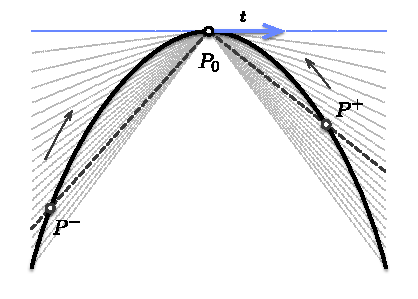
\includegraphics{frenet_tangent.pdf}\label{<figure1>}}
     \subfloat[][Curve's normal and osculating circle.]{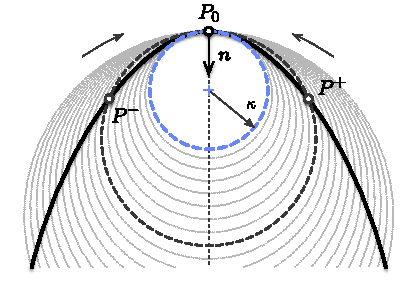
\includegraphics{frenet_normal.pdf}\label{<figure2>}}
     \captionof{figure}[Definition of the tangent vector and the osculating circle of a curve]{Definition of the tangent vector and the osculating circle of a curve.}
     \label{fig:3_1}
\end{figure}

%Normal vector
\subsection{Normal vector}
The second component of the Frenet trihedron is called the \emph{unit normal vector}. It is constructed from $\vect{t'}$ which is necessarily orthogonal to $\vect{t}$. Indeed~:
\begin{equation}
	\norm{\vect{t}}=1 \Rightarrow \vect{t^{'}} \cdot  \vect{t} = 0 \Leftrightarrow  \vect{t^{'}} \perp \vect{t}
	\label{eq:tt}
\end{equation}
Remark that for a curve parametrized by arc length \cref{eq:tt} implies that $\gamma'(s) \cdot \gamma''(s) = 0$.

Let $\gamma = (I,F)$ be a biregular parametric curve. Let $t \in I$ be a parameter. The \emph{unit normal vector} is defined as~: \footnote{Note that $\vect{n}$ exists if only $\gamma$ is biregular, that is $\vect{t}'$ never vanishes, or equivalently $\gamma$ is never locally a straight line. In that case the Frenet trihedron is undefined.}
\begin{equation}
	\vect{n}(t) = \frac{\vect{t}'(t)}{\norm{\vect{t}'(t)}} 
	\quad,\quad
	\norm{\vect{n}(t)}=1
	\label{eq:def_normal}
\end{equation}
Using \cref{eq:def_tangent} in \cref{eq:def_normal} plus the usual derivation rules leads to~: \footnote{Recall that $\gamma'(t) \times (\gamma''(t) \times \gamma'(t)) = \gamma''(t) (\gamma'(t) \cdot \gamma'(t)) - \gamma'(t) (\gamma''(t) \cdot \gamma'(t))$ and that $\norm{\gamma'(t)} = \sqrt{\gamma'(t) \cdot \gamma'(t)}$.}
\begin{equation}
	\vect{t}'(t) = \frac{\gamma'(t) \times (\gamma''(t) \times \gamma'(t))}{\norm{\gamma'(t)}^3}
	\label{eq:tangent_prime}
\end{equation}
Because $\gamma'(t)$ and $\gamma''(t) \times \gamma'(t)$ are perpendicular the following identity holds~:
\begin{equation}
	\norm{\gamma'(t) \times (\gamma''(t) \times \gamma'(t))} = \norm{\gamma'(t)}\norm{\gamma''(t) \times \gamma'(t)}
	\label{eq:identity}
\end{equation}
Thus, combining \cref{eq:tangent_prime,eq:identity} gives~:
\begin{equation}
	\vect{n}(t) = \frac{\gamma'(t) \times (\gamma''(t) \times \gamma'(t))}{\norm{\gamma'(t)}\norm{\gamma''(t) \times \gamma'(t)}}
	\label{eq:def2_normal}
\end{equation}
For a curve parametrized by arc length this expression becomes~:
\begin{equation}
	\vect{n}(s) =  \frac{\gamma''(s)}{\norm{\gamma''(s)}}
	\quad,\quad
	s \in [0,L]
\end{equation}
In differential geometry, the unit normal to the curve $\gamma$ at point $P_0$ is obtained as the limit of the (normalized) vector $\overrightarrow{P_0 P^+}-\overrightarrow{P_0 P^-}$, as $P^-$ and $P^+$ approche $P_0$ respectively from its left and right sides (\cref{fig:3_1})~:
\begin{equation}
	\vect{n}(P_0)
	= \lim_{}\frac{\overrightarrow{P_0 P^+}-\overrightarrow{P_0 P^-}}{\norm{\overrightarrow{P_0 P^+}-\overrightarrow{P_0 P^-}}}
\label{eq:3_4}
\end{equation}
Remark that the notion of \emph{normal vector} is ambiguous for non-planar curves as there is an infinite number of possible normal vectors lying in the plane orthogonal to the curve's tangent. In practice, the tangent derivative is a convenient choice as it allows to extend the notion of curvature from planar to non-planar space curves. However, we will see in \cref{sec:bishop} that other kinds of trihedron can be constructed regarding this choice and that one of them is especially suitable for the study of slender beams.

%Binormal vector and torsion
\subsection{Binormal vector}
The third vector of Frenet's trihedron is called the \emph{unit binormal vector}. It is constructed from $\vect{t}$ and $\vect{n}$ to form an orthonormal direct basis of $\mathbb{R}^{3}$. 
Let $\gamma = (I,F)$ be a biregular parametric curve. Let $t \in I$ be a parameter. The \emph{unit binormal vector} is defined as~:
\begin{equation}
	\vect{b}(t) = \vect{t}(t) \times \vect{n}(t)
	\quad,\quad
	\norm{\vect{b}(t)}=1
	\label{eq:def_binormal}
\end{equation}
Combining \cref{eq:def_tangent} and \cref{eq:def2_normal} with \cref{eq:def_binormal} leads to~:
\begin{equation}
	\vect{b}(t) = \frac{\gamma'(t) \times \gamma''(t)}{\norm{\gamma'(t) \times \gamma''(t)}}
\end{equation}
For a curve parametrized by arc length, this expression becomes~: \footnote{For an arc length parametrized curve the following identity holds : $\norm{\gamma'(s) \times \gamma''(s)} = \norm{\gamma'(s)} \norm{\gamma''(s)}$.}
\begin{equation}
	\vect{b}(s) = \vect{t}(s) \times \vect{n}(s)
	= \frac{\gamma'(s) \times \gamma''(s)}{\norm{\gamma''(s)}}
	\quad,\quad
	s \in [0,L]
\end{equation}

% Osculating plane
\subsection{Osculating plane}\label{sec:osculatingplane}
The tangent and normal unit vectors $\{\vect{t},\vect{n}\}$ form an orthonormal basis of the so-called \emph{osculating plane}, whereas the binormal vector $(\vect{b})$ is orthogonal to it. This plane is of prime importance because it is the plane in which the curve takes its curvature (see \cref{sec:curvature}).

As reported in~\cite[p.45]{Delcourt2007}, the osculating plane seems to have been first introduced by Bernoulli as the plane passing through three infinitely near points on a curve.\footnote{\blockcquote[p.113]{Bernoulli1728}{Voco autem planum osculans, quod transit per tria curvae quaesitae puncta infinite sibi invicem propinqua}.
} Likewise, in modern differential geometry, the osculating plane is defined as the limit of the plane passing through the points $P^-$, $P_0$ and $P^+$ while $P^-$ and $P^+$ approche $P_0$ respectively from its left and right side (\cref{fig:3_1}).

Note that the normal unit vector and the binormal unit vector $\{\vect{n},\vect{b}\}$ define the so-called \emph{normal plane}, while the normal tangent vector and the binormal unit vector $\{\vect{t},\vect{b}\}$ define the so-called \emph{rectifying plane}. These planes are secondary for the present study.

% --------------------------------------------------------------------------------------------------------------------------------------------
% CURVE INVARIANTS
% --------------------------------------------------------------------------------------------------------------------------------------------

\section{Curves of double curvature}\label{sec:curves_of_dc}

The study of space curves belongs to the field of differential geometry. According to~\cite[p.28]{Delcourt2007}, the terminology \emph{curve of double curvature} is attributed to Pitot around 1724.\footnote{\blockcquote[p.28]{Pitot1726}{Les Anciens ont nommé cette courbe Spirale ou Hélice~; parce que la formation sur le cylindre suit la même analogie que la formation d’une spirale ordinaire sur un plan; mais elle est bien différente de la spirale ordinaire, étant une des courbes à double courbure, ou une des lignes qu’on conçoit tracée sur la surface des Solides. Peut-être que ces sortes de courbes à double courbure, ou prises sur la surface des Solides, feront un jour l’objet des recherches des géomètres. Celle que nous venons d’examiner est, je crois, la plus simple de toutes.
}} However, as stated in~\cite[p.321]{Coolidge2013} curvature and torsion where probably first thought by Monge around 1771.\footnote{\blockcquote[p.363]{Monge1809}{On appelle point d'inflexion, dans une courbe plane, le point où cette ligne, après avoir été concave dans un sens, cesse de l'être pour devenir concave dans l'autre sens. Il est évident que dans ce point, la courbe perd sa courbure, et que les deux élémens consécutifs sont en ligne droite. Mais une courbe à double courbure peut perdre chacune de ses courbures en particulier, ou les perdre toutes deux dans le même point~; c'est-à-dire, qu'il peut arriver ou que trois élémens consécutifs d'une même courbe à double courbure se trouvent dans un même plan, ou que deux de ces élémens soient en ligne droite. Il suit de là que les courbes à double courbure peuvent avoir deux espèces d'inflexions~; la première a lieu lorsque la courbe devient plane, et nous l'appellerons simple inflexion~; la seconde, que nous appellerons double inflexion, a lieu lorsque la courbe devient droite dans un de ses points.}.} It is also interesting to note that, at that time, \textquote{curvature} was also referred to as \textquote{flexure}, reflecting that the study of physical problems (e.g. \emph{the elastica}) and the study of curves of double curvature were intimately related to each other.

Space curves were historically understood as \emph{curves of double curvature} by extension to the case of planar curves, where the curvature measures the deviance of a curve from being a straight line. The second curvature, nowadays known as the \textquote{torsion} or \textquote{second generalized curvature}, measures the deviance of a curve from being planar. 

%\note{arclength is a Euclidean invariant of the curve.}

\begin{figure}[t]
	\centering
	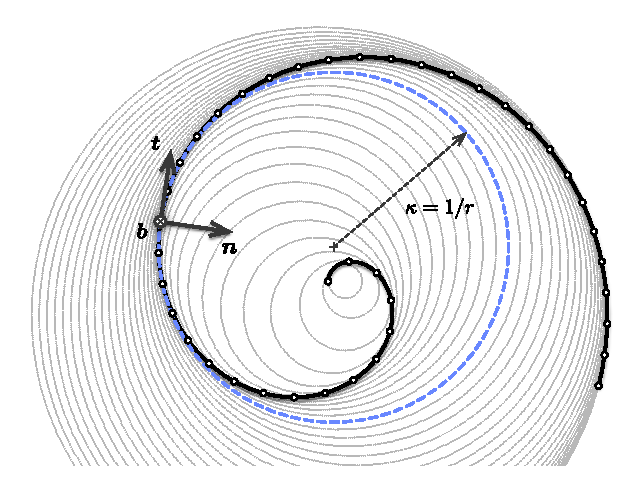
\includegraphics[]{osculating_circle.pdf}
	\captionof{figure}[Osculating circles for a spiral curve at different parameters]{Osculating circles for a spiral curve at different parameters.}
	\label{fig:3_2}
\end{figure}

%Curvature
\subsection{First invariant~: the curvature}\label{sec:curvature}
In differential geometry, the \emph{osculating circle} is defined as the limit of the circle passing through the points $P^-$, $P_0$ and $P^+$ while $P^-$ and $P^+$ approche $P_0$ (\cref{fig:3_1}). This circle lies on the osculating plane and its radius is nothing but the inverse of the local curvature of a curve.\footnote{As explained by Euler himself, at a given arc length parameter ($s$), the osculating plane is the plane in which a curve takes its curvature~: \blockcquote[p.364]{Euler1775}{in quo bina fili elementa proxima in curvantur}.} While the tangent gives the best local approximation of the curve as a straight line, the osculating circle gives the best local approximation of that curve as an arc.

The curvature is also known to be the \emph{gradient of arc length} (see~\cite[p.4]{Vouga2014}) and calculated as~: $\nabla{L} = \kappa \vect{n}$. Thus, the curvature gives the first-order variation in arc length when deforming a curve $\gamma$ into the curve $\gamma + \epsilon \delta\gamma$~:
\begin{subequations}
	\begin{alignat}{2}
		& L(\gamma + \epsilon \delta\gamma) = L(\gamma) + \epsilon (\nabla L \cdot \delta\gamma) + o(\epsilon)
		\\[0.5em]
		& \nabla L \cdot \delta\gamma = \frac{d}{d\epsilon}L(\gamma+\epsilon \delta \gamma)\Bigr|_{\epsilon = 0}
		= \int_0^L \kappa (\delta \gamma \cdot \vect{n})
	\end{alignat}
\end{subequations}
This is easily understood in the case of a circle of radius $r$ extended to a circle of radius $r+dr$, where the total arc length variation is given by~: 
$L(r + dr) - L(r) = \kappa dr L(r) $.

Note that due to the inner product with the normal vector, only the normal component of the deformation results in an effective extension of the curve. This point is worth to note as it will be related to the \emph{inextensibility assumption} made later in our beam model (see \cref{sec:}).

\subsubsection{Curvature}
Let $\gamma$ be a regular arc length parametrized curve. Let $s \in [0,L]$ be an arc length parameter. The \emph{curvature} is a positive scalar quantity defined as~:
\begin{equation}
	\kappa(s) = \norm{\vect{t}'(s)} \ge 0 
	\quad,\quad
	\vect{t}'(s) = \kappa(s) \vect{n}(s)
\label{eq:curvaturedef}
\end{equation}
The curvature is \emph{independent} regarding the choice of parametrization. This makes the curvature an \emph{intrinsic property} of a given curve and that is why it is also referred to as a \emph{geometric invariant}. Following~\cite[pp.203-204]{Gray2006} it can be computed for any parametrization $(I,F)$ of $\gamma$ as~:
\begin{equation}
	\kappa(t) = \frac{\norm{\gamma'(t) \times \gamma''(t)}}{\norm{\gamma'(t)}^3}
	\quad,\quad
	\vect{t}'(t) = \norm{\gamma'(t)} \kappa(t) \vect{n}(t)
\label{eq:curvaturedef2}
\end{equation}
Note that in \cref{eq:curvaturedef} the prime symbol denotes the derivative with respect to the natural parameter ($s$) while in \cref{eq:curvaturedef2} it denotes the derivative with respect to any parameter ($t$). Consequently, the \emph{speed} of the curve's parametrization appears in the latter equation~:
\begin{equation}
	v(t) = \frac{ds}{dt} = \norm{\gamma'(t)} = s'(t)
\end{equation}
The curvature measures how much a curve bends instantaneously in its osculating plane, that is how fast the tangent vector is rotating in the osculating plane around the binormal vector. In differential geometry this is expressed for a planar curve as~:
\begin{equation}
	\kappa(s)
	= \lim_{ds \to 0}\frac{\angle(\vect{t}(s),\vect{t}(s+ds))}{ds}
	= \lim_{ds \to 0}\frac{(\vect{t}(s+ds) - \vect{t}(s)) \cdot \vect{n}(s)}{ds}
\end{equation}
where $\angle(\vect{t}(s),\vect{t}(s+ds))$ denotes the angle between $\vect{t}(s)$ and $\vect{t}(s+ds)$. This is equivalent as measuring how fast the osculating plane itself is rotating around the binormal vector. Consequently a curve is locally a \emph{straight line} when its curvature vanishes ($\kappa(s)= 0$).

%Radius of curvature
\subsubsection{Radius of curvature}
The \emph{radius of curvature} is defined as the inverse of the curvature ($r= 1/\kappa$). From a geometric point of view, one can demonstrate that it is the radius of the osculating circle (see \cref{fig:3_2}). Remark that where the curvature vanishes the radius of curvature goes to infinity~; that is the osculating circle becomes a line, a circle of infinite radius.

%Osculating circle
\subsubsection{Center of curvature}
The \emph{center of curvature} is defined as the center of the osculating circle (see \cref{fig:3_2}). The locus of all the centers of curvature of a curve is called the \emph{evolute}.

\subsubsection{Curvature binormal vector}
\label{sec:kb}
Finally, following~\cite{Bergou2008} we define the \emph{curvature binormal vector}. Let $\gamma$ be a biregular arc length parametrized curve. Let $s\in [0,L]$ be an arc length parameter. The \emph{curvature binormal vector} is defined as~:
\begin{equation}
	\vect{\kappa b}(s) = \kappa(s)\cdot\vect{b}(s) = \vect{t}(s) \times \vect{t}'(s)
	\quad,\quad
	\norm{\vect{\kappa b}(s)}= \kappa(s)
\label{eq:kb}
\end{equation}
This vector will be useful as it embed all the necessary information on the curve's curvature. We will see in \cref{sec:bishopvelocity} that this vector is associated to the angular velocity of a specific adapted moving frame attached to the curve and called the \emph{Bishop frame}.

% Torsion
\subsection{Second invariant~: the torsion}\label{sec:torsion}
Let $\gamma$ be a biregular arc length parametrized curve. Let $s \in [0,L]$ be an arc length parameter. The \emph{torsion} is a scalar quantity defined as~:
\begin{equation}
	\tau_f(s) = \vect{n}'(s) \cdot \vect{b}(s) = - \vect{b}'(s) \cdot \vect{n}(s)
\end{equation}
The torsion is \emph{independent} regarding the choice of parametrization. This makes the torsion an \emph{intrinsic property} of a given curve and that is why it is also referred to as a \emph{geometric invariant}. Following~\cite[p.204]{Gray2006} it can be computed for any parametrization $(I,F)$ of $\gamma$ as~:
\begin{equation}
	\tau_f(t) = \frac{\gamma'(t) \cdot (\gamma''(t)) \times \gamma'''(t))}{\norm{\gamma'(t) \times \gamma''(t)}^2}
	\quad when \quad
	\kappa(t) > 0
\end{equation}
The torsion measures how much a curve goes \emph{instantaneously out of its plane}, that is to say how fast the normal or binormal vectors are rotating in the normal plane around the tangent vector. In differential geometry this is expressed as~:
\begin{equation}
	\tau_f(s) 
	= \lim_{ds \to 0}\frac{\angle(\vect{n}(s),\vect{n}(s+ds))}{ds}
	= \lim_{ds \to 0}\frac{(\vect{n}(s+ds) - \vect{n}(s)) \cdot \vect{b}(s)}{ds}
\end{equation}
This is equivalent as measuring how fast the osculating plane is rotating around the tangent vector. Consequently a curve is locally \emph{plane} when its torsion vanishes ($\tau_f(s) = 0$).

Remark that the \emph{torsion} is denoted \textquote{$\tau_f$} and not simply \textquote{$\tau$} as the latter will be reserved to denote any angular velocity of a moving adapted frame around its tangent vector. Thus, $\tau_f$ refers to the particular angular velocity of the Frenet trihedron around its tangent vector. This torsion, which is a geometric property of the curve, will be indifferently referred to as the \emph{Frenet torsion} or the \emph{geometric torsion}.

% Fundamental theorem of space curves
\subsection{Fundamental theorem of space curves}\label{sec:fundamental}
This two \emph{generalized curvatures}, respectively the curvature ($\kappa$) and the torsion ($\tau_f$), are \emph{invariant} regarding the choice of parametrization and under \emph{euclidean motions}. The \emph{Fundamental theorem of space curves} states that a curve is fully described, up to a Euclidean motion of ${\mathbb{R}}^3$, by its positive curvature ($\kappa > 0$) and torsion ($\tau_f$)~\cite[p.229]{Gray2006}.

% The Serret-Frenet formulas
\subsection{Serret-Frenet formulas}\label{sec:serret}
The \emph{Fundamental theorem of space curves} is somehow a consequence of the \emph{Serret-Frenet formulas}, which is the first-order system of differential equations satisfied by the Frenet trihedron. Let $\gamma$ be a biregular arc length parametrized curve. Let $s \in [0,L]$ be an arc length parameter. Then, the Frenet trihedron satisfies the following formulas~:
\begin{subequations}
	\begin{alignat}{2}
		&\vect{t^{'}}(s) 	&&=  \kappa_{}(s) \vect{n}(s)
		\\
		&\vect{n^{'}}(s) 	&&=  -\kappa_{}(s) \vect{t}(s) + \tau_f(s) \vect{b}(s)
		\\
		&\vect{b^{'}}(s) 	&&=  -\tau_f(s) \vect{n}(s)
	\end{alignat}
\end{subequations}
This system can be seen as the \emph{equations of motion} of the Frenet trihedron moving along the curve $\gamma$ at unit speed ($\norm{\gamma'}=1$). Indeed, introducing its \emph{angular velocity vector} also known as the \emph{Darboux vector} ($\vect{\Omega_f}$), the previous system is expressed as~:
\begin{equation}
	\begin{bmatrix}		
		\vect{t^{'}}(s) \\
		\vect{n^{'}}(s) \\
		\vect{b^{'}}(s) \\
	\end{bmatrix}
	=
	\vect{\Omega_f}(s)
	\times
	\begin{bmatrix}		
		\vect{t}(s) \\
		\vect{n}(s) \\
		\vect{b}(s) \\
	\end{bmatrix}
	\quad where \quad
	\vect{\Omega_f}(s)
	=
	\begin{bmatrix}
		\tau_f(s) \\
		0 \\
		\kappa(s)
	\end{bmatrix}
\end{equation}
Because the Frenet trihedron satisfies a first-order system of differential equations of parameters $\kappa$ and $\tau_f$ it is possible, by integration, to reconstruct the trace of the moving frame and thus the curve, up to a constant of integration (a trihedron in this case).
%For instance, those classic combinations of curvature and torsion leads to~:
%\begin{itemize}
%	\item a curve of null curvature and null torsion is a straight line ;
%	\item a curve of constant curvature and null torsion is a circle ;
%	\item a curve of constant curvature and constant torsion is a circular helix.
%\end{itemize}

Finally, those formulas can be generalized to any non unit-speed parametrization of a curve.\footnote{See~\cite[p.203]{Gray2006} for a complete proof.} Let $\gamma = (I,F)$ be a biregular parametric curve. Let $t \in I$ be a parameter. Then the following \emph{generalized Serret-Frenet formulas} hold~:
\begin{subequations}
	\begin{alignat}{2}
		&\vect{t^{'}}(t) 	&&=  v(t) \kappa_{}(t) \vect{n}(t)
		\\
		&\vect{n^{'}}(t) 	&&=  -v(t) \kappa_{}(t) \vect{t}(t) + v(t) \tau_f(s) \vect{b}(t)
		\\
		&\vect{b^{'}}(t) 	&&=  -v(t) \tau_f(t) \vect{n}(t)
	\end{alignat}
\end{subequations}
Again, this system can be seen as the \emph{equations of motion} of the Frenet trihedron moving along the curve $\gamma$ at non unit-speed ($v(t) = \norm{\gamma'(t)}$). This time the \emph{angular velocity vector} ($\vect{\Omega}$) is distinct from the \emph{Darboux vector} ($\vect{\Omega_f}$) and the previous system is expressed as~:
\begin{equation}
	\begin{bmatrix}		
		\vect{t^{'}}(t) \\
		\vect{n^{'}}(t) \\
		\vect{b^{'}}(t) \\
	\end{bmatrix}
	=
	\vect{\Omega}(t)
	\times
	\begin{bmatrix}		
		\vect{t}(t) \\
		\vect{n}(t) \\
		\vect{b}(t) \\
	\end{bmatrix}
	\quad where \quad
	\vect{\Omega}(t)
	=
	v(t)
	\begin{bmatrix}
		\tau_f(t) \\
		0 \\
		\kappa(t)
	\end{bmatrix}
\end{equation}


\begin{figure}[t]
	\centering
	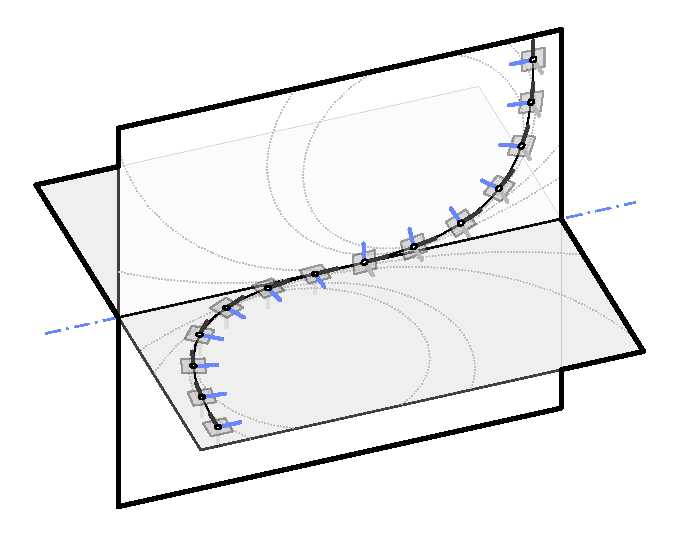
\includegraphics[]{frenet_torsion.pdf}
	\captionof{figure}[Discontinuity of the Frenet trihedron at an inflexion point]{Discontinuity of the Frenet trihedron at an inflexion point where the curvature vanishes and the orientation of the osculating plane is subject to a jump of angle $\pi/2$.}
	\label{fig:3_3}
\end{figure}

% --------------------------------------------------------------------------------------------------------------------------------------------
% CURVE FRAMING
% --------------------------------------------------------------------------------------------------------------------------------------------

\section{Curve framing}\label{sec:curve_framing}

%From now on, we consider $\gamma$ to be a biregular arc length parametrized curve.

While the Frenet trihedron \blockcquote[p.1]{Bishop1975}{has long been the standard vehicle for analysing properties of the curve invariant\footnote{Namely the curvature ($\kappa$) and the Frenet torsion ($\tau_f$).} under euclidean motions}, a curve can be potentially framed with any arbitrary \emph{moving frame}, understood as an \emph{orthonormal basis field}. Thus, the Frenet frame is not the only way to frame a curve and other frames may also exhibit some interesting properties.\footnote{Recall the title of Bishop's paper~: \blockcquote[]{Bishop1975}{There is more than one way to frame a curve}.} 

In his paper~\cite{Bishop1975} Bishop establishes the differential equation that a moving frame must satisfy and remarks that, because of the orthonormality condition, the first derivatives of the frame components can be expressed in terms of themselves through a skew-symmetric coefficient matrix. For such a frame, the understanding of its motion along the curve is thus reduced to the knowledge of only three scalar coefficient functions. He remarks that most of the interesting properties that the Frenet frame exhibits are due to the fact that one of these coefficient functions is vanishing everywhere on the curve (that is the frame is \emph{rotation-minimizing} regarding one of its components)~; and that the Frenet frame is \emph{adapted} to the curve (that is one of its components is nothing but the unit tangent vector).

In this section we introduce the notion of \emph{moving frame} and two properties of interest that such a frame can exhibit in addition, namely~: to be \emph{adapted} to the curve ; and to be \emph{rotation-minimizing} regrading a given direction. We then reconsider the case of the Frenet frame regrading this mathematical framework. Finally, we introduce the \emph{zero-twisting} frame also known as the \emph{Bishop} frame.\footnote{Named after Bishop who introduced it.} This tool will be fundamental for our futur study of slender beams.

% moving frame
\subsection{Moving frame}\label{sec:moving_frame}

Let $\gamma$ be a curve parametrized by arc length. A map $F$ which associates to each point of arc length parameter $s$ a direct orthonormal trihedron is said to be a \emph{moving frame}~:
\begin{equation}
	\fonctionL{F}{[0,L]}{\mathcal{SO}_{3}(\mathbb{R})}{s}{F(s) = \{\vect{e}_{3}(s),\vect{e}_{1}(s),\vect{e}_{2}(s)\}}
\end{equation}
Note that a direct orthonormal trihedron (or basis) is an element of the \emph{rotation group} denoted $\mathcal{SO}_{3}$.
Consequently, a moving frame $F$ attached to $\gamma$ satisfies for all $s \in [0,L]$~:
\begin{subequations}
	\begin{alignat}{2}
		& \norm{\vect{e}_i(s)} = 1 
		\\
		& \vect{e}_i(s) \cdot \vect{e}_j(s) = 0\quad , \quad i \neq j
	\end{alignat}
\end{subequations}
The term \textquote{moving frame} will refer indifferently to the map itself (denoted $F=\{\vect{e}_{3},\vect{e}_{1},\vect{e}_{2}\}$), or to a specific evaluation of the map (denoted $F(s)=\{\vect{e}_{3}(s),\vect{e}_{1}(s),\vect{e}_{2}(s)\}$). 

At first sight this indexing could seem strange but it will be convenient later in our mechanical model where $\vect{e}_{3}$ will be associated to the centerline's tangent and $\vect{e}_{1}$ and $\vect{e}_{2}$ to the two cross-section principal axes of inertia. These axes will also be called \emph{material axes}. We chose to introduce this indexing right now to maintain consistency between notations through out the chapters of this manuscript.

% governing equations
\subsubsection{Governing equations}
Computing the derivatives of the previous relationships leads to the following system of differential equations that the frame must satisfy for all $s \in [0,L]$~:
\begin{subequations}
	\begin{alignat}{2}
		&\vect{e}'_i(s) \cdot \vect{e}_i(s) = 0 
		\\
		&\vect{e}'_{i}(s) \cdot \vect{e}_{j}(s) = -\vect{e}_{i}(s) \cdot \vect{e}'_{j}(s)\quad , \quad i \neq j
	\end{alignat}
\end{subequations}
Thus, there exists 3 scalar functions ($\tau$, $k_{1}$, $k_{2}$) such that $\{\vect{e}'_{3}, \vect{e}'_{1}, \vect{e}'_{2}\}$ can be expressed in the basis $\{\vect{e}_{3}, \vect{e}_{1}, \vect{e}_{2}\}$~:
\begin{subequations}
%	\left\{
	\begin{alignat}{2}
		&\vect{e}'_{3}(s) &&= k_{2}(s)\vect{e}_{1}(s) - k_{1}(s)\vect{e}_{2}(s) \\
		&\vect{e}'_{1}(s) &&= -k_{2}(s)\vect{e}_{3}(s) + \tau(s)\vect{e}_{2}(s) \\
		&\vect{e}'_{2}(s) &&= k_{1}(s)\vect{e}_{3}(s) - \tau(s)\vect{e}_{1}(s)
	\end{alignat}
%	\right.
\end{subequations}
It is common to rewrite this first-order linear system of differential equations as a matrix equation~: \footnote{In the case of a space curve, where $\vect{e}_3$ is chosen to be the curve tangent unit vector and $\vect{e}_1$ is chosen to be the curve normal unit vector, this set of equations is known as the \emph{Serret-Frenet formulas}.}\textsuperscript{,}\footnote{In the case of a space curve drawn on a surface, where $\vect{e}_3$ is chosen to be the curve tangent unit vector and $\vect{e}_1$ is chosen to be the surface normal unit vector, this set of equations is known as the \emph{Darboux-Ribaucour formulas}.}
\begin{equation}
	\begin{bmatrix}
		\vect{e}'_{3}(s) \\
		\vect{e}'_{1}(s) \\
		\vect{e}'_{2}(s)
	\end{bmatrix}
	=
	\begin{bmatrix}
		0 & k_{2}(s) & -k_{1}(s) \\
		-k_{2}(s) & 0 & \tau(s) \\
		k_{1}(s) & -\tau(s) & 0
	\end{bmatrix}
	\begin{bmatrix}
		\vect{e}_{3}(s) \\
		\vect{e}_{1}(s) \\
		\vect{e}_{2}(s)
	\end{bmatrix}
\label{eq:movingframe}
\end{equation}
Since the progression of any moving frame along $\gamma$ is ruled by a first-order system of differential equations, a unique triplet $\{\tau, k_{1}, k_{2}\}$ leads to a set of moving frames equal to each other within a constant of integration.\footnote{This assumption reminds the \emph{Fundamental theorem of space curves} (\cref{sec:fundamental}).} Basically, with a given triplet $\{\tau, k_{1}, k_{2}\}$, one can propagate a given initial direct orthonormal trihedron (at $s=0$ for instance) through the whole curve by integrating the system of differential equations. In general, a moving frame will be fully determined by $\tau$, $k_{1}$ and $k_{2}$ together with the initial condition $\{\vect{e}_{3}(s=0),\vect{e}_{1}(s=0),\vect{e}_{2}(s=0)\}$.

\begin{figure}[t]
\centering
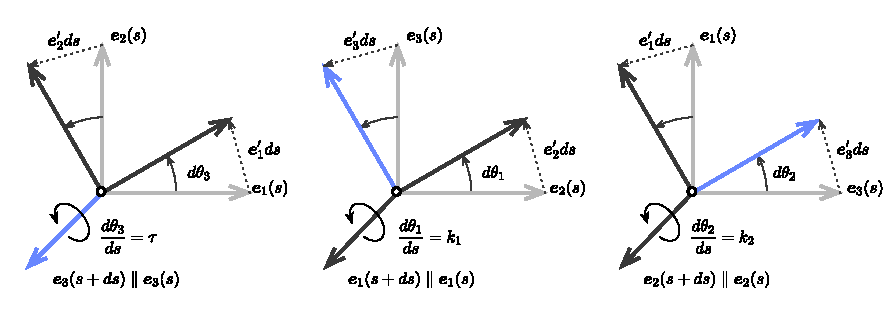
\includegraphics[]{darboux.pdf}
\captionof{figure}[Geometric interpretation of the angular velocity vector of a moving frame]{Geometric interpretation of the angular velocity vector of a moving frame.}
\label{fig:geo_interpretation}
\end{figure}

% ANGULAR VELOCITY VECTOR
\subsubsection{Angular velocity}
This system can be seen as the \emph{equations of motion} of the frame moving along the curve $\gamma$ at unit speed ($\norm{\gamma'}=1$). Indeed, introducing its \emph{angular velocity vector} ($\vect{\Omega}$), the previous system is expressed as~:
\begin{equation}
	\vect{e}'_{i}(s) = \vect{\Omega}(s) \times \vect{e}_{i}(s)
	\quad avec \quad
	\vect{\Omega}(s)
	=
	\begin{bmatrix}
		\tau(s) \\
		k_1(s) \\
		k_2(s)
	\end{bmatrix}
\end{equation}
This result is straightforward deduced from \cref{eq:movingframe}. Note that the cross product reveals the skew-symmetric nature of the system, which could already be seen in \cref{eq:movingframe}.
Geometrically, decomposing the infinitesimal rotation of the moving frame around its directors between arc length $s$ and $s+ds$ (see \cref{fig:geo_interpretation}) shows that the scalar functions $\tau$, $k_{1}$ and $k_{2}$ effectively correspond to the angular speed of the frame moving along $\gamma$, respectively around $\vect{e}_{3}$, $\vect{e}_{1}$ and $\vect{e}_{2}$~:
\begin{subequations}
	\begin{alignat}{2}
		&\frac{d\theta_3}{ds}(s) &&= \tau(s)
		\\[0.5em]
		&\frac{d\theta_1}{ds}(s) &&= k_{1}(s)
		\\[0.5em]
		&\frac{d\theta_2}{ds}(s) &&= k_{2}(s)
	\end{alignat}
\end{subequations}

\begin{figure}[t]
\centering
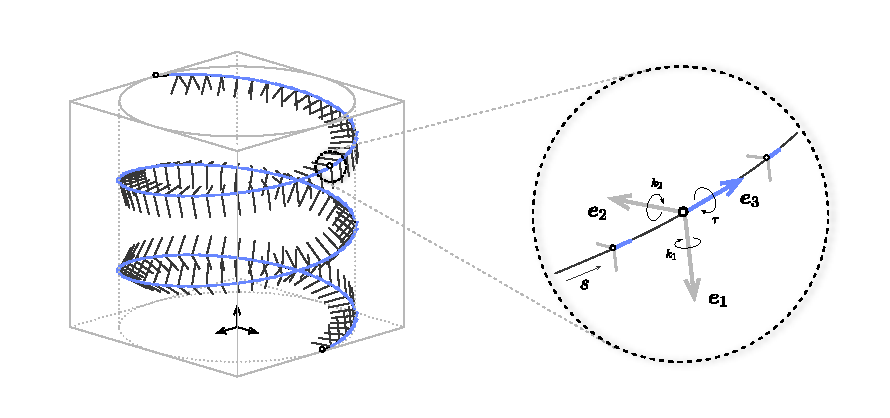
\includegraphics[]{adapted_moving_frame.pdf}
\captionof{figure}[Adapted moving frame on a circular helix]{Moving frame $F(s) =\{\vect{e}_{3}(s),\vect{e}_{1}(s),\vect{e}_{2}(s)\}$ on a circular helix. The frame is adapted as $\vect{e}_3(s) = \vect{t}(s)$.}
\label{fig:adapted}
\end{figure}

% ADAPTED FRAME
\subsection{Adapted moving frame}\label{sec:amf}

Let $F$ be a moving frame as defined in the previous section. $F$ is said to be \emph{adapted} to $\gamma$ if at each point $\gamma(s)$, $\vect{e}_{3}(s)$ is the unit tangent vector of $\gamma$ (\cref{fig:adapted})~:
\begin{equation}
	\vect{e}_{3}(s) = \vect{t}(s) = \gamma^{'}(s)
\end{equation}
For an adapted frame, the components $k_1$ and $k_2$ of the angular velocity vector are related to the curvature of $\gamma$~: \footnote{This is why for an initially straight rod with an isotropic cross-section bending and torsion are uncoupled. Indeed, in that case the bending energy does not depend on the orientation of the cross-sections anymore as it depends only on the curvature of the rod~: $\mathcal{E}_b = EI_1\kappa_1^2 + EI_2\kappa_2^2 = EI\kappa^2$.}
\begin{equation}
	\kappa(s) = \norm{\vect{e}'_{3}(s)} = \norm{k_2(s)\vect{e}_1(s) + k_1(s)\vect{e}_2(s)} = \sqrt{{k_{1}(s)}^2 + {k_{2}(s)}^2}
	\label{eq:kb_components}
\end{equation}
Moreover, recalling the definition of the curvature binormal vector ($\vect{\kappa b}$) from \cref{eq:kb}, it is easy to see that for an adapted moving frame the following relation holds~:
 \begin{equation}
	\vect{\kappa b}(s) = k_1(s) \vect{e}_1(s) +  k_2(s) \vect{e}_2(s) \label{eq:amf_kb}
\end{equation}
Consequently, the angular velocity vector of an adapted moving frame can be written as~:
 \begin{equation}
	\vect{\Omega}(s) = \vect{\kappa b}(s)  + \tau(s) \vect{t}(s)
	\label{eq:angular_velocity}
\end{equation}
This last result is very interesting as it shows that any adapted moving frame will differ from each other only by their twisting speed, as $\vect{\Omega}_{\perp} =  \vect{\kappa b}$ only depends on the curve.

% ROTATION MINIMIZING FRAME
\subsection{Rotation-minimizing frame}
Following~\cite{Farouki2014, Wang2008} we introduce the \emph{rotation-miniminzing frame} notion. A frame $\{\vect{e}_{3}$, $\vect{e}_{1}$, $\vect{e}_{2}\}$ is said to be \emph{rotation-miniminzing} regrading a given direction $\vect{d}$ if~:
\begin{equation}
	\vect{\Omega}(s) \cdot \vect{d}(s) = 0
\end{equation}

% PARALLEL TRANSPORT
\subsection{Parallel transport}\label{sec:paralleltransport}
The notion of \emph{parallel transport} is somehow a generalization of the classical notion of collinearity in flat euclidean spaces (e.g.\ $\mathbb{R}^2$ or $\mathbb{R}^3$), to spaces that exhibit some non vanishing curvature (e.g.\ spheric or hyperbolic spaces).\footnote{\url{https://www.youtube.com/watch?v=p1tfZD2Bm0w}}

\subsubsection{Relatively parallel fields}
Following~\citef{Bishop1975}, we define what is a \emph{(relatively) parallel field}. Let $\gamma$ be a regular curve parametrized by arc length. Let $\vect{p}$ be a vector field along $\gamma$. The vector field $\vect{p}$ is said to be \emph{parallel} if its derivative is purely tangential, that is~:
\begin{equation}
	\vect{p}'(s) \times \vect{t}(s) = 0
\end{equation}
Consequently, for an adapted moving frame, the \emph{normal fields} $\vect{e}_1$ and $\vect{e}_2$ are both \emph{relatively parallels} if and only if the frame angular velocity is itself a normal field, that is~: \footnote{A vector field $\vect{p}$ is said to be \emph{normal} along a curve $\gamma$ if~: $\forall s \in [0,L]$, $\vect{p}\cdot\vect{t} = 0$.}
\begin{equation}
	\vect{\Omega}(s) = \vect{\Omega}_{\perp}(s) =  \vect{\kappa b}(s) \Leftrightarrow \vect{\Omega}(s) \cdot \vect{t}(s) = 0  \Leftrightarrow \tau(s) = 0  
\end{equation}
In other words, a \emph{relatively parallel normal field}~: \blockcquote{Bishop1975}{turns, only whatever amount is necessary for it to remain normal, so it is as close to being parallel as possible without losing normality}. 
%
%In addition, relatively parallel normal vector fields exhibit some interesting properties~\cite{Hanson95}~: 
%\begin{itemize}
%	\item $\|\vect{p}\|$ is of constant length;
%	\item $\|\vect{p}\|$ is of constant length;
%\end{itemize}

\subsubsection{Parallel transport of vectors along a curve}
Reciprocally, it is possible to define the \emph{parallel transport} of a vector along a curve $\gamma$ as its propagation along $\gamma$ at angular speed $\vect{\kappa b}$. An initial vector $\vect{p}_0 = \vect{p}(s_0)$ is parallel transported at arc length parameter $s$ into the vector $\vect{p}(s)$ by integrating the following first-order differential equation along $\gamma$~:
\begin{equation}
	\vect{p}'(s) = \vect{\kappa b}(s) \times  \vect{p}(s)
\end{equation}
Consequently, the resulting vector field $\vect{p}$ is a parallel field. Note that a parallel field is not necessarily a normal field. 

From the point of view of differential geometry, this means that the next vector $\vect{p}(s+ds)$ is obtained by rotating the previous one $\vect{p}(s)$ around the curve binormal $\vect{b}(s)$ by an infinitesimal angle $d\theta(s) = \kappa(s) ds$. Note that $\vect{b}(s)$ has the same direction as $\vect{t}(s) \times \vect{t}(s+ds)$.

\subsubsection{Parallel transport of frames along a curve}
Identically, the \emph{parallel transport} of an adapted frame is defined as the parallel transport of its components along $\gamma$.

%\subsubsection{Parallel curves and inextensibility}
%Let $\vect{p}$ be a \emph{relatively parallel normal vector field}.
%
%Relatively parallel fields~\cite[p.4]{Carroll2007},~\cite{Bishop1975},~\cite{Hanson95}

% FRENET FRAME
\subsection{Frenet frame}
\label{sec:ff}

The Frenet frame is a well-known particular adapted moving frame. It is defined as the map that attach to any given point of $\gamma$ the corresponding Frenet trihedron $\{\vect{t}(s),\vect{n}(s),\vect{b}(s)\}$ where~:
\begin{subequations}
	\begin{alignat}{2}
		&\vect{t}(s) = \gamma^{'}(s)
		\\[0.5em]
		&\vect{n}(s) = \frac{\vect{t'}(s)}{\kappa(s)}
		\\[0.5em]
		&\vect{b}(s)= \vect{t}(s)\times\vect{n}(s)
	\end{alignat}
\end{subequations}

\subsubsection{Governing equations}\label{sec:serretfrenet}
The Frenet frame satisfies the \emph{Frenet-Serret formulas} (see \cref{sec:serret}), which govern the evolution of the frame along the curve $\gamma$~:
\begin{equation}
	\begin{bmatrix}
		\vect{t^{'}}(s) \\
		\vect{n^{'}}(s) \\
		\vect{b^{'}}(s)
	\end{bmatrix}
	=
	\begin{bmatrix}
		0 & \kappa_{}(s) & 0 \\
		-\kappa_{}(s) & 0 & \tau_f(s) \\
		0 & -\tau_f(s) & 0
	\end{bmatrix}
	\begin{bmatrix}
		\vect{t}(s) \\
		\vect{n}(s) \\
		\vect{b}(s)
	\end{bmatrix}
\label{eq:frenetframegoverning}
\end{equation}
Remember the generic system of differential equations of an adapted moving frame attached to a curve, established in \cref{eq:movingframe}, where $\vect{e}_{3}(s) = \vect{t}(s)$, $k_{1}(s) = 0$, $k_{2}(s) = \kappa(s)$ and $\tau(s)= \tau_{f}(s)$.

\subsubsection{Angular velocity}
Consequently, the angular velocity vector ($\vect{\Omega_{f}}$) of the Frenet frame, also known as the \emph{Darboux vector} in this particular case, is given by~:
\begin{equation}
	\vect{\Omega_f}(s)
	=
	\begin{bmatrix}
		\tau_{f}(s) \\
		0 \\
		\kappa(s)
	\end{bmatrix}
	= \vect{\kappa b}(s) +\tau_{f}(s) \vect{t}(s)
\end{equation}
Remark that the Frenet frame satisfies $\vect{\Omega_f}(s) \cdot \vect{n}(s) = 0$ and is thus a \emph{rotation-miniminzing} frame regarding the normal vector ($\vect{n}$). The motion of this frame through the curve is known as \emph{pitch-free}.

Note also that $\vect{t^{'}}(s)$ and $\vect{b^{'}}(s)$ are collinear to $\vect{n}(s)$. This means that the projection of $\vect{t}(s)$ and $\vect{b}(s)$ is conserved from one normal plane to another, that is $\vect{t}$ and $\vect{b}$ are parallel transported along the vector field $\vect{n}$.

\subsubsection{Drawbacks and benefits}\label{sec:frenetdrawbacks}
%\footnote{\note{une perturbation de la courbe dans le sens de la courbure engendre une variation de longueur de la courbe proportionnelle à l'inverse de la courbure (au premier ordre) + schéma.}}\textsuperscript{,}\footnote{\note{une perturbation de la courbe dans le sens de la binormale (en tout point) préserve la longueur de la courbe au 1er ordre~: c'est un déplacement qui conserve l'hypothèse d'inextensibilité au premier ordre.}}\textsuperscript{,}\footnote{\note{Examiner la question de la fermeture sur une boucle fermée. Schéma.}}

The Frenet frame is not continuously defined if $\gamma$ is not $\mathcal{C}^2$. This is problematic for the study of slender beams as the centerline of a beam subject to punctual external forces and moments or to material discontinuities will not be $\mathcal{C}^2$ but only picewise $\mathcal{C}^2$. In that case, the centerline tangent will be continuously defined everywhere but the curvature will be subject to discontinuities, that is $\vect{t}'$ will not be continuously defined.

Moreover, even if $\gamma$ is $\mathcal{C}^2$, the Frenet frame is not defined where the curvature vanishes, which obviously is an admissible configuration for a beam centerline. This issue can be partially addressed by parallel transporting the normal vector along the straight regions of the curve. Thus, the extended frame will still satisfy the governing equations exposed in \cref{eq:frenetframegoverning}. However, if the osculating planes are not parallels on both sides of a region of null curvature, torsion will be subject to a discontinuity and so the Frenet frame (\cref{fig:3_3}).\footnote{This is also highlighted in~\cite{Bloomenthal1990, Wang2008}.} Again, if the region of null curvature is not a point, that is the region is not an inflexion point but a locus where the curve is locally a straight line, the change in torsion on both sides of the region can be accommodated by a continuous rotation from one end to the other.

One benefit of the Frenet frame is that, when transported along a \emph{closed curve}, the frame at the end of the curve will align back with the frame at the beginning of the curve, that is the frame will returns to its initial value after a complete turn. During its trip, the frame will make a total twist of $\int_0^L \tau_f(s)ds = 0[2\pi]$ around the tangent vector.

A second benefit is that any adapted frame can be obtained by a rotation of the Frenet frame around the unit tangent vector~\cite[p.2]{Guggenheimer1989}.

% BISHOP FRAME
\subsection{Bishop frame}\label{sec:bishop}

A \emph{Bishop frame} denoted $\{\vect{t},\vect{u},\vect{v}\}$, also known as \emph{zero-twisting} or \emph{parallel-transported} frame, is an adapted moving frame that has no tangential angular velocity~: \footnote{Bishop frames were introduced as \emph{relatively parallel adapted frames} in~\cite{Bishop1975}.}
\begin{equation}
	\vect{\Omega} \cdot \vect{t} = \tau =\vect{u^{'}} \cdot \vect{v} = - \vect{u} \cdot \vect{v^{'}} = 0
	\label{eq:null_velocity}
\end{equation}
Because a Bishop frame is an adapted frame, it can be defined relatively to the Frenet frame by a rotation around the unit tangent vector. A Bishop frame is a frame that cancels out the rotational movement of the Frenet frame around the tangent vector. At arc length parameter $s$, the Frenet frame has continuously rotated around its tangent vector of a cumulative angle~: $\int_0^s \tau_f(t)dt$. Thus, any Bishop frame will be obtained, within a constant rotation angle $\theta_0$, through a rotation of the Frenet frame around the tangent vector by an angle~:
\begin{equation}
	\theta(s)  =  - \int_0^s \tau_f(t)dt + \theta_0(s)
\end{equation}
Consequently, a Bishop frame can be expressed relatively to the Frenet frame as~:
\begin{equation}
	\left\{
	\begin{aligned}
		&\vect{u} = \cos \theta \vect{n} +  \sin \theta \vect{b}\\
		&\vect{v} = -\sin \theta \vect{n} +  \cos \theta \vect{b}
	\end{aligned}
	\right.
\end{equation}
\subsubsection{Governing equations}
The Bishop frame satisfies the following system of differential equations, which governs the evolution of the frame along the curve $\gamma$~:
\begin{equation}
	\begin{bmatrix}
		\vect{t^{'}}(s) \\
		\vect{u^{'}}(s) \\
		\vect{v^{'}}(s)
	\end{bmatrix}
	=
	\begin{bmatrix}
		0 & \kappa(s) \sin \theta(s) & -\kappa(s) \cos \theta(s) \\
		-\kappa(s) \sin \theta(s) & 0 & 0 \\
		\kappa(s) \cos \theta(s) & 0 & 0
	\end{bmatrix}
	\begin{bmatrix}
		\vect{t}(s) \\
		\vect{u}(s) \\
		\vect{v}(s)
	\end{bmatrix}
\label{eq:3_12}
\end{equation}
One can remember the generic differential equations of an adapted moving frame attached to a curve, where~: \footnote{
\begin{equation*}
	\begin{aligned}
		&\tau =\vect{u^{'}} \cdot \vect{v} = (\vect{\Omega_f} \times \vect{u} + \theta^{'} \vect{v})\cdot  \vect{v} = \tau_f - \tau_f = 0\\
		&k_1 = -\vect{t^{'}} \cdot \vect{v} = -\kappa \vect{n} \cdot \vect{v} = \kappa \sin \theta \\
		&k_2 = \vect{t^{'}} \cdot \vect{u} = \kappa \vect{n} \cdot \vect{u} = \kappa \cos \theta
	\end{aligned}
\end{equation*}
}
\begin{equation}
k_{1}(s) = \kappa(s) \sin \theta(s)
\quad,\quad
k_{2}(s) = \kappa(s) \cos \theta(s)
\quad,\quad
\tau(s) = 0
\end{equation}

\subsubsection{Angular velocity}\label{sec:bishopvelocity}
Consequently, the angular velocity vector ($\vect{\Omega_{b}}$) of the Bishop frame is given by~:
\begin{equation}
	\vect{\Omega_b}(s) 
	=
	\begin{bmatrix}
		0\\
		\kappa(s) \sin \theta(s)\\
		\kappa(s) \cos \theta(s)
	\end{bmatrix}
	= \vect{\kappa b}(s) 
\end{equation}
Remark that the Bishop frame satisfies $\vect{\Omega_b}(s) \cdot \vect{t}(s) = 0$ and is thus \emph{rotation-miniminzing} regarding the tangent vector. The motion of this frame through the curve is known as \textquote{roll-free}.

Because the motion of this frame is described by an angular velocity vector that is nothing but the curvature binormal vector ($\vect{\Omega_b} = \vect{\kappa b}$), it can be interpreted in terms of \emph{parallel transport} as defined in \cref{sec:paralleltransport}. Thus, given an initial frame at arc length parameter $s=0$, the Bishop frame at any arc length parameter ($s$) is obtained by parallel transporting the initial frame $\{\vect{t}(0),\vect{u}(0), \vect{v}(0)\}$ along the curve from $0$ to $s$.

\subsubsection{Drawbacks and benefits}
One of the main benefits of the Bishop frame is that its generative method~: \blockcquote{Bloomenthal1990}{is immune to degeneracies in the curvature vector}. Although we first expressed the construction of the Bishop frame relatively to the Frenet frame (which exists wherever $\gamma$ is biregular), the existence of the Bishop frame, understood in terms of parallel transport, is guaranteed wherever the curvature binormal ($\vect{\kappa b} = \vect{t} \times \vect{t}'$) is defined. To be continuously defined over $[0,L]$, a Bishop frame only needs the curvature binormal vector to be piecewise continuously defined over  $[0,L]$, which only requires that $\gamma'$ is $\mathcal{C}^0$ and that $\gamma''$ is piecewise $\mathcal{C}^0$. Obviously, those weaker existence conditions are profitables to bypass the drawbacks of the Frenet frame regarding the modeling of slender beams listed in \cref{sec:frenetdrawbacks}.

Strictly speaking, a Bishop frame is not a reference frame as it is defined within an initial condition. However, we will see later that strains in a beam are modeled as a rate of change in the Bishop frame, and consequently the initial condition will disappear in the equations.

Unlike the Frenet frame, when transported along a \emph{closed curve}, the Bishop frame at the end of the curve will not necessarily align back with the frame at the beginning of the curve.\footnote{\blockcquote{Hanson95}{it is possible for closed curves to have parallel transport frames that do not match up after one full circuit of the curve}.} Even if the frame returns to its initial value after a complete turn, it may returns in its position after several complete turns ($2k\pi$) around the curve tangent. During its movement along the curve, the frame will make a total twist of $\int_0^L \tau_f(s)ds = \alpha[2\pi]$ around the tangent vector. This difference of angle is related to the concept of \emph{holonomy}.

Remark also that Frenet and Bishop frames coincide for planar curves ($\tau_f = 0$), within a constant rotation around the unit tangent vector.
 
 %related to mechanical torsion

%expliquer la notion de parallèle comme l'a formulé Laurent Hauswirth~: la projection de $u'$ et $v'$ dans le plan normal à la tangente $t$ est nulle, cad que d'un plan à un autre la projection de $u$ et $v$ est conservée + faire schéma.

%Laurent Hauswirth~: la complexité d'un problème est en général proportionnelle à la codimension de l'objet étudié et donc, de ce fait les courbes ($codim = 3-1 = 2$) sont des objets plus compliqués que les surfaces ($codim = 3-2=1$) ds $\mathbb{R}^3$.

\subsection{Comparison between Frenet and Bishop frames}
Let $\gamma$ be a \emph{circular helix} of parameter $a$ and $k$. In a cartesian coordinate system, it is defined as~:
\begin{equation}
	\vect{r}(t) 
	=
	\begin{bmatrix}
		a \cos t, a \sin t, k t
	\end{bmatrix}
	= a \cos t \, \vect{e}_x + a \sin t \, \vect{e}_y + k t \, \vect{e}_z
\end{equation}
The speed of this parametrization, the curvature and the geometric torsion are uniform and given by~:
\begin{subequations}
	\begin{alignat}{2}
		&v(t) &&= \sqrt{a^2+k^2}
		\\
		&\kappa(t) &&= \frac{a}{a^2 + k^2}
		\\	
		&\tau_f(t) &&= \frac{k}{a^2 + k^2}
	\end{alignat}
\end{subequations}
The Frenet frame components are given by (with $\alpha = v \kappa$ and $\beta = v \tau_f$)~:
\begin{subequations}
	\begin{alignat}{2}
		&\vect{t}(t) &&=
		\begin{bmatrix}  - \alpha \cos t, \alpha \sin t, \beta t  \end{bmatrix}
		\\
		&\vect{n}(t) &&=  \begin{bmatrix}  -\cos t, -\sin t, 0  \end{bmatrix}
		\\
		&\vect{b}(t) &&= \begin{bmatrix}  \beta \sin t, - \beta \cos t, \alpha \end{bmatrix} 	
	\end{alignat}
\end{subequations}
And the Bishop frame components are given by~:
\begin{subequations}
	\begin{alignat}{1}
		\vect{u}(t) &= \begin{bmatrix} 	
			-\cos t \cos \beta t - \beta  \sin t \sin \beta t, -\sin t \cos \beta t + \beta  \cos t \sin \beta t, - \alpha \sin \beta t
			\end{bmatrix}
		\\
		\vect{v}(t) &= \begin{bmatrix} 
			-\cos t \sin \beta t + \beta  \sin t \cos \beta t, -\sin t \sin \beta t - \beta  \cos t \cos \beta t, \alpha \cos \beta t
		\end{bmatrix}
	\end{alignat}
\end{subequations}
At $t=0$ the two frames coincide. At $t>0$ the Bishop frame is obtained from the Frenet frame by a rotation around $\vect{t}(t)$ of an angle $\theta(t) = - \tau_f \cdot (v t)$.  

The angular velocities of the Frenet and Bishop frames are respectively given by~:
\begin{subequations}
	\begin{alignat}{2}
		&\vect{\Omega}_f(t) &&= \begin{bmatrix} \tau_f , 0, \kappa \end{bmatrix}
		\\
		&\vect{\Omega}_b(t) &&= \begin{bmatrix} 0 , \kappa \sin \theta, \kappa \cos \theta \end{bmatrix}
	\end{alignat}
\end{subequations}

\begin{figure}[p]
\centering
	\vspace{-0.5cm}
	\subfloat[][Frenet frame]{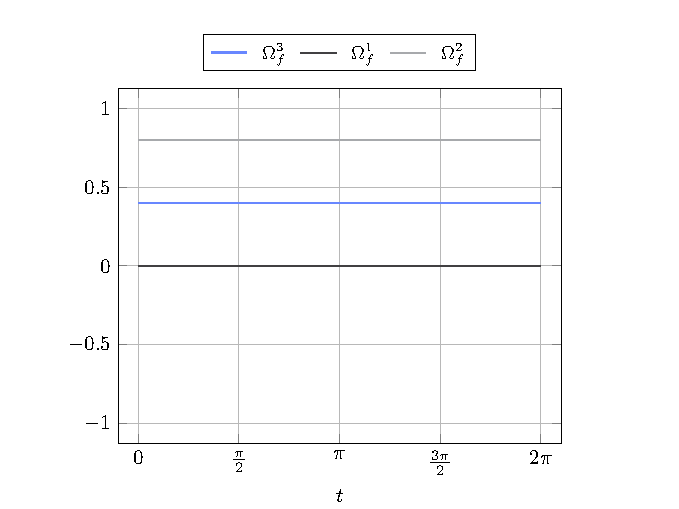
\includegraphics[]{ch4_geometry/plot/1_bench_frame/build_frenet.pdf}\label{plot:frenet}}
	\\
%  	 \hspace{0.2cm}
	\subfloat[][Bishop frame]{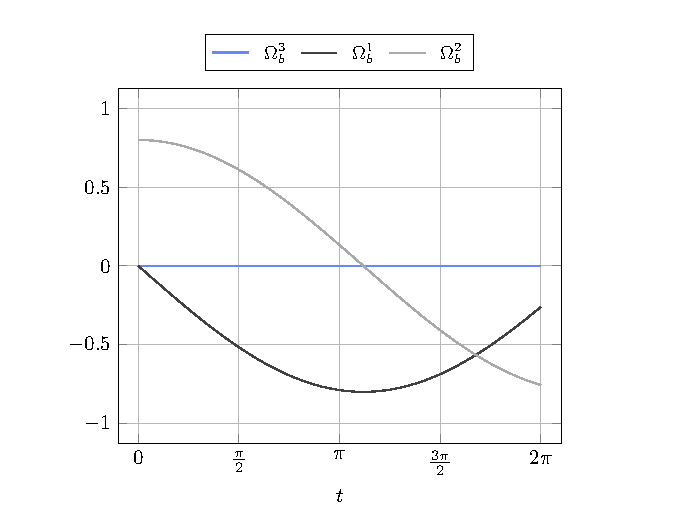
\includegraphics[]{ch4_geometry/plot/1_bench_frame/build_bishop.pdf}\label{plot:bishop}}
	\captionof{figure}[Angular velocities of Frenet and Bishop frames for a circular helix]{Angular velocities of Frenet and Bishop frames for a circular helix ($a=1.0$ and $k=0.5$).}
	\label{fig:frame_bench}
\end{figure}
The components of these angular velocities are plotted in \cref{fig:frame_bench} for a circular helix with parameter $a=1.0$ and $k=0.5$ while the parameter $t$ varies from $0$ to $2\pi$. At $t=2\pi$ the frame has made a full turn and its altitude has increased from $0$ to $\pi$. 

The components of the angular velocity of the Frenet frame are constant during the movement along the curve and the frame does not rotate around the normal vector as $\Omega_f^2 = 0$ (see \cref{plot:frenet}). The components of the angular velocity of the Bishop frame vary during the movement along the curve and the frame does not rotate around the tangent vector as $\Omega_b^3 = 0$ (see \cref{plot:bishop}).

% DISCRETE CURVES
% ================
\section{Discrete curves}\label{sec:discrete_curves}

The previous section has introduced the fundamental analytical tools to develop a solid understanding of the geometry of smooth space curves. These tools will be essentials for the construction of the beam model presented later in \cref{sec:energy} and \cref{sec:krichhoff}. In this section we look for equivalent notions in the case of discrete space curves, as the developed model will be implemented in a numerical program to solve real mechanical problems through discrete element models (see \cref{sec:discretization}).

The study of those discrete equivalent notions belong to the recent field of \emph{Discrete Differential Geometry}~: \blockcquote[p.7]{Hoffmann2008}{In some sense discrete differential geometry can be considered more fundamental than differential geometry since the later can be obtained form the former as a limit}. In particular, we will see that they are several ways to define the discrete equivalents of the curvature and the unit tangent vector. Though these various ways are equivalent and match their smooth counterpart by passing to the limit, they exhibit different capabilities at the discrete level.

 \blockcquote[p.1]{Carroll2014}{There is no general theory or methodology in the literature, despite the ubiquitous use of discrete curves in mathematics and science. There are conflicting definitions of even basic concepts such as discrete curvature $\kappa$, discrete torsion $\tau$, or discrete Frenet frame.}.

%\cite{Hoffmann2008, Carroll2014, Crane2015, Vouga2014}

% definition
% ------------
\subsection{Definition}

Let $\Gamma$ be a discrete (or polygonal) space curve. $\Gamma$ is defined as an ordered sequence $\Gamma = (\vect{x}_0,  \vect{x}_1, \ldots, \vect{x}_n) \in \mathbb{R}^{3(n+1)}$ of $n+1$ pairwise disjoint \emph{vertices} (see \cref{fig:discrete_curve}). Consecutive pairs of vertices define $n$ straight segments $(\vect{e}_0,  \vect{e}_1, \ldots, \vect{e}_{n-1})$ called \emph{edges}, pointing from one vertex to the next one~: $\vect{e}_i = \vect{x}_{i+1} - \vect{x}_{i}$. The midpoint of $\vect{e}_i$ is a vertex denoted~: $\vect{x}_{i+1/2} = \vect{x}_{i} + \frac{1}{2}\vect{e}_{i}$.

The length of $\vect{e}_i$ is denoted $l_i = \norm{\vect{e}_i}$. The total length of $\Gamma$ is denoted $L = \sum_{i=0}^{n-1} \norm{\vect{e}_i}$. Additionally, we define the vertex-based mean length \overbar{l_i} at vertex $\vect{x}_i$~: 
\begin{equation}
%\setlength{\jot}{8pt}
	\left\{
	\begin{alignedat}{4}
		\,	&\overbar{l_0} 		& = &\,	&& l_0					&\quad 	&i = 0		\\
			&\overbar{l_i}		& = &	&& \frac{1}{2}(l_{i-1} + l_i)		&		&i \in \llbracket 1, n-1 \rrbracket	\\
			&\overbar{l_n} 	\,	& = &	&& l_{n-1} 				&		&i = n		\\
	\end{alignedat}
	\right.
\end{equation}

\begin{figure}[t]
	\centering
	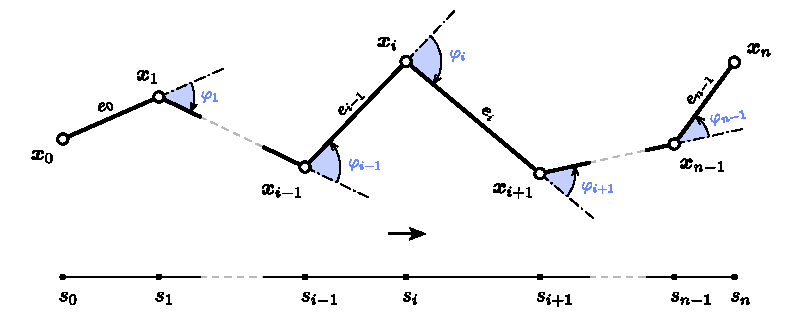
\includegraphics[]{discrete_curve_full.pdf}
	\captionof{figure}[Discrete curve representation and parametrization]{Discrete curve representation and parametrization.}
	\label{fig:discrete_curve}
\end{figure}

\subsubsection{Discrete unit tangent vector}\label{sec:tangent_edge}
Edge vectors lead to a natural definition of the \emph{discrete unit tangent vector} along each edge~: $\vect{u}_i = \vect{e}_i / l_i$. However, this definition makes no sense at vertices where all the curvature is condensed and measured by the turning angle ($\varphi_i$). This is often illustrated in terms of the Gau{\ss} map, a transformation in which edges will map to points and vertices will map to curves on the unit sphere.

\subsubsection{Discrete osculating plane}
Consecutive pairs of edges lead to a natural definition of the \emph{discrete osculating plane}, as the plane in which $\Gamma$ locally lies on. This plane is well defined by its normal vector known as the \emph{discrete unit binormal vector} ($\vect{b}_i = \frac{\vect{e}_{i-1} \times \vect{e}_{i}}{\norm{\vect{e}_{i-1} \times \vect{e}_{i}}}$) only if $\vect{e}_{i-1}$ and $\vect{e}_{i}$ are non-collinear ; that is the curve is not locally a straight line, or equivalently the curvature does not vanish.

\subsubsection{Discrete turning angle}
The \emph{turning angle} is defined as the oriented angle between to adjacent edges~: $\varphi_i=\angle(\vect{e}_{i-1},\vect{e}_i)$. It is defined only for all $i \in \llbracket1,n-1\rrbracket$. It corresponds to the angle of rotation, in the osculating plane, around the binormal vector ($\vect{b}_i$), to align $\vect{e}_{i-1}$ with $\vect{e}_{i}$. The sign of $\varphi_i$ is taken in accordance to the right-hand rule regarding the orientation of $\vect{b}_i$. Thus, $\varphi_i$ is necessarily bounded to $[0,\pi]$~:
\begin{equation}
	0 \leqslant \varphi_i \leqslant \pi
\end{equation}
The next section will highlight the central role of the turning angle in the possible measurements of the discrete curvature.

Recall that for a planar curve, where $\varphi$ denotes the angle between the tangent vector ($\vect{t} = \cos\varphi \,\vect{e}_x + \sin\varphi \,\vect{e}_y$) and the horizontal line of direction $\vect{e}_x$, the following relation holds~: $\varphi(s_1) - \varphi(s_2) = \int_{s_1}^{s_2} \frac{d \varphi}{d s} ds = \int_{s_1}^{s_2} \kappa ds$.

% parametrization
% ---------------------
\subsection{Regularity}

Let $\Gamma = (\vect{x}_0,  \vect{x}_1, \ldots, \vect{x}_n)$ be a discrete curve of edges $\vect{e}_0,  \vect{e}_1, \ldots, \vect{e}_{n-1}$. $\Gamma$ is said to be~:
\begin{itemize}
	\item  \emph{regular} if it has no kinks~: $\vect{e}_{i-1} + \vect{e}_{i} \neq 0 \Leftrightarrow \varphi_i \neq \pi \; | \; \forall i \in \llbracket 1,n-1 \rrbracket $
	\item  \emph{biregular} if no vertex is flat~: $\vect{e}_{i-1} - \vect{e}_{i} \neq 0 \Leftrightarrow \varphi_i \neq 0 \; | \; \forall i \in \llbracket 1,n-1 \rrbracket $
\end{itemize}

% parametrization
% ---------------------
\subsection{Parametrization}

In the literature, discrete curves are usually considered as maps defined on $I = \llbracket 0,n \rrbracket \in \mathbb{N}^{n+1}$. As a consequence, the discrete derivative of $\Gamma$ is an edge-based quantity defined as~: 
\begin{equation}
	\Gamma'_i = \frac{ \Gamma(t_{i+1}) -  \Gamma(t_i)}{t_{i+1} - t_i} = \vect{e}_i 
	\quad , \quad
	\vect{x}_{i} = \Gamma(t_i)
	\quad , \quad
	t_i = i
\end{equation}
Thus, as in the smooth case, a discrete curve is said to be parametrized by arc length if $\norm{\Gamma'} = 1$, that is every edges are of unit length ($\norm{\vect{e}_i} = 1$).\footnote{This assumption leads to the assertion that \blockcquote[p.10]{Hoffmann2008}{A discrete curve is parameterized by arc length or it is not}.} This constraint is sometimes relaxed to curves of constant edge length ($\norm{\vect{e}_i} = c$) that are said to be parametrized \emph{proportional} to arc length.

In the present work, to stick closer to the smooth case, we instead consider discrete curves as maps defined on $I = [t_0, t_1, \ldots, t_n] \in \mathbb{R}^{n+1}$ where $t$ denotes the discrete parametrization of $\Gamma$. As in the smooth case, the way to parametrized a curve is not unique.

\subsubsection{Arc length parameter}
By analogy with the smooth case, we define the curve arc length at vertices (see \cref{fig:discrete_curve}) as~:
\begin{equation}
	\left\{
	\begin{aligned}
		s_0 	&= 0 								& 	&i = 0		\\
		s_i 	&= \sum_{k=1}^i \norm{\vect{e}_{k-1}}		&	&i \in \llbracket 1, n-1 \rrbracket	\\
		s_n 	&=  L 								&	&i = n		\\
	\end{aligned}
	\right.
\end{equation}
This definition naturally extends to the whole domain by piecewise linear interpolation. This is not different as considering the discrete curve as a continuous polygonal curve. Indeed, for any $s \in [s_i, s_{i+1}]$ there exists a normalized parameter $t = \frac{s - s_i}{s_{i+1} - s_i} \in [0,1]$ so that~:
\begin{subequations}
	\begin{alignat}{2}
		&s(t) &= (1-t) s_i + t s_{i+1} = s_i + t l_i 
		\\
		&\vect{x}(t) &= (1-t) \vect{x}_i  + t \vect{x}_{i+1} =  \vect{x}_i + t  \vect{e}_i
	\end{alignat}
\end{subequations}
Note that this parametrization satisfies $\norm{\Gamma'}=1$ on $\bigcup_{i=1}^n ]s_{i-1}, s_i[$ but $\Gamma'$ remains undefined at vertices. This issue is the reason why defining the tangent vector at vertices can not be done unequivocally for discrete curves.

% DISCRETE CURVATURE
% ===================
\section{Discrete curvature}\label{sec:discrete_curvature}
\citef{Vouga2014} defines and compares three different definitions of the discrete curvature that does not suppose that $\norm{\vect{e}_i}$ is constant. By trying to mimic some properties of the curvature in the smooth case \citef{Carroll2014} and \citef{Bobenko2015} also define and compare three different definitions of the discrete curvature from the osculating circle. One main drawback of all the said proposals is that the question of the curvature at  start and end points is never treated. But this is of main importance when dealing with beams as the nature of the boundary conditions can make the curvature to be null or not at its ends, depending if somme moment has to be transfer or not. In this sens, the question of discrete curvature could not be treated separately with the question of the tangent vector.

\subsection{Definition from osculating circles}
Curvature is defined from the osculating circle, which is the best approximation of a curve by a circle.

\begin{figure}[p]
\centering
\renewcommand{\arraystretch}{1.5}
		\vspace{-0.5cm}
		\subfloat[][vertex-based]{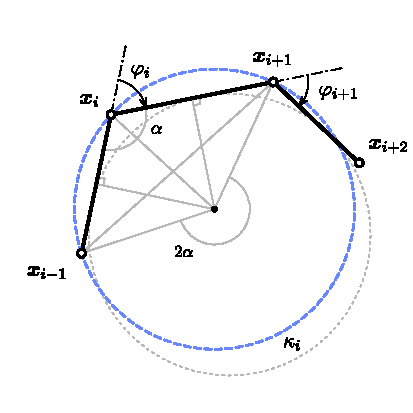
\includegraphics{kb_vertex.pdf}\label{fig:kb_vertex}}\hspace{5mm}
    		\subfloat[][edge-based]{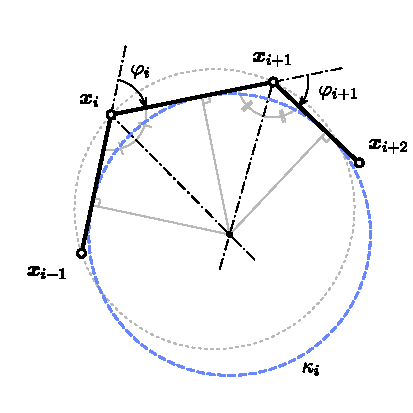
\includegraphics{kb_edge.pdf}\label{fig:kb_edge}} \\[-10pt]
		\subfloat[][bitangent with $\norm{\vect{e}_{i-1}}$]{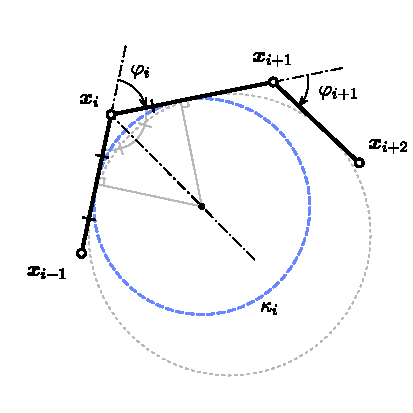
\includegraphics{kb_mixed_a.pdf}\label{fig:kb_mixed_a}}\hspace{5mm}
		\subfloat[][bitangent with $\norm{\vect{e}_{i}}$]{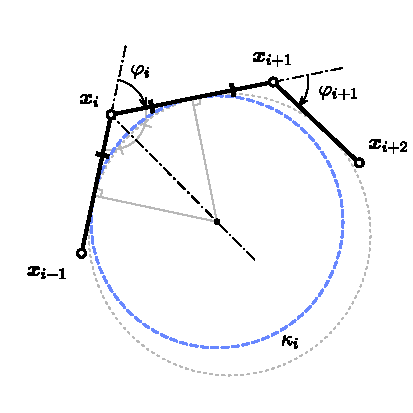
\includegraphics{kb_mixed_b.pdf}\label{fig:kb_mixed_b}}
		\vspace{10pt}
		\captionof{figure}[]{Several ways to define the osculating circle for discrete curves, leading to different notions of discrete curvature.}
		\label{fig:kb_def}
		\vspace{0.75cm}
		\ra{1.5}
 		\begin{tabularx}{0.9\textwidth}{@{} X c c c r r r @{}}
      		\toprule
		Curvature ($\kappa_i$) 										&  Locality 	&  $\varphi \mapsto 0$ 	&  $\varphi \mapsto \pi$ 		& Ends  	& Dim 	&  Fitting			\\
		\midrule
		$\kappa_1 = \frac{2\, \sin(\varphi_i)}{\norm{\vect{e}_{i-1}+\vect{e}_i}}$ 	&  $\vect{x}_i$ 	&  $0$				&  $0, 2$					&  yes	&  space	&  clothoid			\\
		$\kappa_2 = \frac{\tan(\varphi_i/2)+\tan(\varphi_{i+1}/2)}{l_i}$ 			&  $\vect{e}_i$ 	&  $0$				&  $\infty$					&  no		&  planar	&  circle			\\
 		$\kappa_3 = \frac{2\, \tan(\varphi_i / 2)}{\overbar{l_i}} $				&  $\vect{x}_i$	&  $0$ 				&  $\infty$					&  no		&  space	&  circles			\\
		\midrule
		$\kappa_4 = \frac{2\,\sin(\varphi_i / 2)}{\overbar{l_i}}$ 				&  $\vect{x}_i$	&  $0$				&  $0, 2$					&  no		&  space	&  clothoid  		\\
		$\kappa_5 = \frac{\varphi_i}{\overbar{l_i}}$ 						&  $\vect{x}_i$	&  $0$				&  $\pi/\overbar{l_i}$			&  no		&  space	&  elastica  		\\
		\bottomrule
		\end{tabularx}
		\vspace{10pt}
		\captionof{table}[Review of several discrete curvature definitions]{Review of several discrete curvature definitions mentioned in the literature.}
		\label{tab:kb_def}
\end{figure}

%
%\afterpage{%    % defer execution until the next page break occurs anyway
%	\clearpage
%   	\begin{figure}[t!] % not "pt"
%      		\centering
%		\vspace{-5mm}
%      		% remaining contents of figure environment
%		\subfloat[][vertex-based]{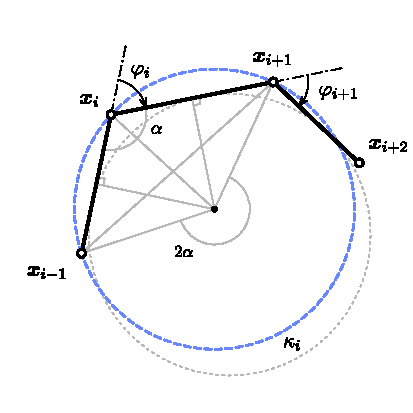
\includegraphics{kb_vertex.pdf}\label{fig:kb_vertex}}\hspace{5mm}
%    		\subfloat[][edge-based]{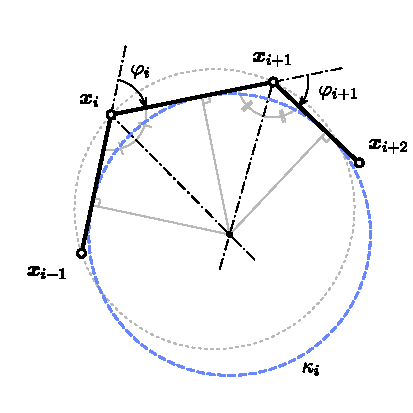
\includegraphics{kb_edge.pdf}\label{fig:kb_edge}} \\[-10pt]
%		\subfloat[][bitangent with $\norm{\vect{e}_{i-1}}$]{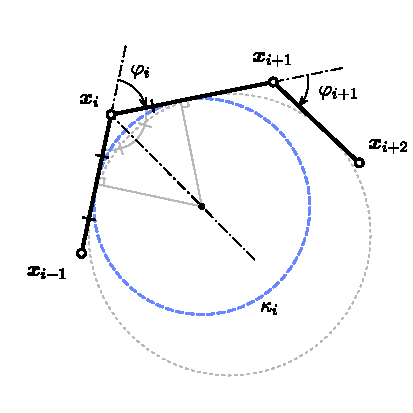
\includegraphics{kb_mixed_a.pdf}\label{fig:kb_mixed_a}}\hspace{5mm}
%		\subfloat[][bitangent with $\norm{\vect{e}_{i}}$]{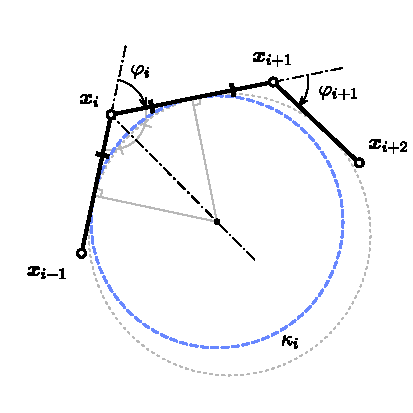
\includegraphics{kb_mixed_b.pdf}\label{fig:kb_mixed_b}}
%		\vspace{10pt}
%		\captionof{figure}[]{Several ways to define the osculating circle for discrete curves, leading to different notions of discrete curvature.}
%		\label{fig:kb_def}
%   	\end{figure}
%   	\begin{table}[h!] % not t or b or p
%		\centering
%      		% remaining contents of table environment
%      		\renewcommand{\arraystretch}{1.5}
% 		\begin{tabular}{l | c c c c c c}
%      		\hline
%		Curvature ($\kappa_i$) 										&  Locality 	&  $\varphi \mapsto 0$ 	&  $\varphi \mapsto \pi$ 		& Ends  	& Dim 	&  Fitting	\\
%		\hline
%		$\kappa_1 = \frac{2\, \sin(\varphi_i)}{\norm{\vect{e}_{i-1}+\vect{e}_i}}$ 	&  $\vect{x}_i$ 	&  $0$				&  $0, 2$					&  yes	&  space	&  clothoid		\\
%		$\kappa_2 = \frac{\tan(\varphi_i/2)+\tan(\varphi_{i+1}/2)}{l_i}$ 			&  $\vect{e}_i$ 	&  $0$				&  $\infty$					&  no		&  planar	&  circle			\\
% 		$\kappa_3 = \frac{2\, \tan(\varphi_i / 2)}{\overbar{l_i}} $				&  $\vect{x}_i$	&  $0$ 				&  $\infty$					&  no		&  space	&  circles			\\[5pt]
%	\hline
%		$\kappa_4 = \frac{2\,\sin(\varphi_i / 2)}{\overbar{l_i}}$ 				&  $\vect{x}_i$	&  $0$				&  $0, 2$					&  no		&  space	&  clothoid  		\\
%		$\kappa_5 = \frac{\varphi_i}{\overbar{l_i}}$ 						&  $\vect{x}_i$	&  $0$				&  $\pi/\overbar{l_i}$			&  no		&  space	&  elastica  		\\[5pt]
%		\hline
%		\end{tabular}
%		\captionof{figure}[]{Review of several discrete curvature definitions mentioned in the literature.}
%	\label{tab:kb_def}
%   \end{table}
%} % end of argument of `\afterpage` command
%

%\footnote{
%Curvature is defined from the osculating circle, which is the best approcximation of a curve by a circle.
%We can define such a circle and it's radius will be the curvature at that point. Problem~: there are several ways to define such a circle.
%
%Très intéressant de constater que cette vision 3 verticies  vs. 2 edges est déjà présente dès le début dans l'histoire de la compréhension de la courbure.
%
%Pour Euler, le rayon de courbure est le rapport de l’élément d’arc sur l’angle de contin-
%gence entre deux tangentes infiniment proches. Par ailleurs, la définition du plan osculateur n’est pas tout à fait lamêmeque chez Bernoulli, plan passant par trois points consécutifs, puis- qu’Euler dit que ce plan contient deux éléments successifs. Il le définit aussi en disant que c’est le plan où la courbe s’incurve. Pour le dire de façon un peu différente~: la tangente contient un élément, c’est le lieu où la courbe est droite, la plan osculateur représente l’étape suivante, c’est le lieu où la courbe est arc de cercle. Nous ne pensons pas trahir Euler en faisant cette présen- tation~: cela justifie que, pour lui, il est naturel de se placer sur le plan osculateur pour calculer le rayon de courbure.~\cite{Delcourt2007}
%
%
%The edge osculating circle.
%The vertex osculating circle.
%La localité est meilleur dans le cas du vertex-based discret osculating circle.
%Pour des anlges élevés, le edge-based discret osculating circle est plus pertinent.
%La courbure tend vers l'infini quand les 2 edges deviennent colineaires.
%
%La définition du plan osculateur est univoque dans le cas discret~: c'est localement le plan défini par 2 edges consécutifs.
%
%Ce n'est pas le cas de la courbure qui perd son côté intrinsèque.
%
%courbure discrete dans le cas général
%}

% vertex-based curvature
% -------------------------------
\subsubsection{Vertex-based osculating circle (circumscribed)}\label{sec:circumscribed}
Let $\Gamma$ be a discrete curve parametrized by arc length. The \emph{vertex-based} (or circumscribed) osculating circle at vertex $\vect{x}_{i}$ is defined as the unique circle passing through the points $\vect{x}_{i-1}$, $\vect{x}_{i}$ and $\vect{x}_{i+1}$ (see \cref{fig:kb_vertex}). This circle leads to the following definition of the curvature~:~\footnote{This curvature is also known as the \emph{Menger curvature}.}
\begin{equation}
	\vect{\kappa b}_i = \frac{2 \, \vect{e}_{i-1} \times \vect{e}_{i}}{\norm{\vect{e}_{i-1}} \norm{\vect{e}_{i}} \norm{\vect{e}_{i-1} + \vect{e}_{i}} }
	\quad , \quad
	\kappa_i = \norm{\vect{\kappa b}_i} = \frac{2 \, \sin(\varphi_i)}{\norm{\vect{e}_{i-1} + \vect{e}_{i}}}
\label{eq:def_kb_vertex}
\end{equation}
This definition shows a good locality as the curvature is attached to the vertex $\vect{x}_{i}$, right in the place where it occurs on the discret curve. In addition, this definition leads to a natural local spline interpolation by the circumscribed osculating circle itself. This interpolation has the advantage to pass exactly through three vertices, to lie on the osculating plane and to share the same curvature as $\Gamma$ at $\vect{x}_{i}$. It also leads to a natural definition of the tangent vector at $\vect{x}_{i}$ (see \cref{sec:tangent}).

Moreover, while this definition is valid only on the current portion of $\Gamma$ ($i \in[1, n-1]$), it is straightforward extended to its endings ($i=0,1$), provided that a unit tangent vector $\vect{t}_{0}$ (respectively $\vect{t}_{n}$) is given at $\vect{x}_{0}$ (resp. $\vect{x}_{n}$), as the unique circle tangent to $\vect{t}_{0}$ (resp. $\vect{t}_{n}$) passing through $\vect{x}_0$ and $\vect{x}_1$ (resp. $\vect{x}_{n-1}$ and $\vect{x}_n$)~:
\begin{equation}
	\vect{\kappa b}_0 = \frac{2 \, \vect{e}_{0} \times \vect{t}_{0}}{\norm{\vect{e}_{0}}^2} 
	\quad , \quad
	\vect{\kappa b}_n = \frac{2 \, \vect{t}_{n} \times \vect{e}_{n-1}}{\norm{\vect{e}_{n-1}}^2} 
\end{equation}
This property will be very profitable in the discrete beam model developed later in the manuscript. It is examined more in details in section \cref{sec:tangent} about the definition of the tangent vector.

However, there are some important drawbacks as the curvature is bounded to $[0,2]$ (see \cref{fig:kb_bench}). When the curve tends to kinks ($\varphi \mapsto \pi$), one would expect the curvature to diverge toward infinity, but instead it tends to a finite value equals to $0$ ($l_{i-1} \neq l_i$) or $2$ ($l_{i-1} = l_i$). This issue can be bypassed if the discretization is refined \textquote{enough}. A criterion is given in the next section (\cref{sec:bench_disc}).

%This expression can be written in a more convenient way for futur comparisons~:
%\begin{equation}
%	\kappa_1 = \frac{2}{\overbar{l_i}} \sin(\varphi_i / 2) \times \beta_i
%	\quad , \quad 
%	\beta_i = 
%%		\frac{\cos(\varphi_i/2)}{\sqrt{1 - \frac{l_{i-1} l_i}{\overbar{l_i} \overbar{l_i}}  \sin^2(\varphi_i/2)}} 
%%		\frac{1}{\sqrt{1 + (1 - \frac{l_{i-1} l_i}{\overbar{l_i} \overbar{l_i}}) \tan^2(\varphi_i/2)}} 
%		\left( 1 + (1 - \frac{l_{i-1} l_i}{\overbar{l_i} \overbar{l_i}}) \tan^2(\varphi_i/2) \right)^{-1/2}
%\end{equation}
%Note that $\beta_i = 1$ for a constant edge length curve ($l_{i-1} = l_i$).

% edge-based curvature
% ------------------------------
\subsubsection{Edge-based osculating circle (inscribed)}
Let $\Gamma$ be a discrete curve parametrized by arc length. The \emph{edge-based} osculating circle at edge $\vect{e}_{i}$ is defined as the unique circle tangent to the edges $\vect{e}_{i-1}$, $\vect{e}_{i}$ and $\vect{e}_{i+1}$ (see \cref{fig:kb_edge}).
\begin{equation}
	\kappa_i = \frac{\tan(\varphi_i/2) + \tan(\varphi_{i+1}/2)}{\norm{\vect{e}_{i}}}
\label{eq:def_kb_edge}
\end{equation}
This definition shows an appropriate behavior~: when the curve tends to kicks the radius of curvature tends to zero ($\tan \varphi/2 \mapsto \infty$), and when the curve tends to be a straight line the curvature tends to $0$ ($\tan \varphi/2 \mapsto 0$).

However, it needs $\Gamma$ to be planar which is by far too restrictive regarding our goal (the modeling of 3D slender beams). Finally, this way of defining the curvature is not as local as one would expect as it is defined relatively to the edge $\vect{e}_{i}$ but not where the turning occurs, at vertices.

% mixed approach
% ---------------------
\subsubsection{Bitangent osculating circle (inscribed)} \label{sec:inscribed}
Let $\Gamma$ be a discrete curve parametrized by arc length. Following~\cite{Vouga2014} we define the curvature regrading the mean length $\overbar{l_i}$ attached to $\vect{x}_{i}$ as~: \footnote{This definition is also presented in~\cite{Bobenko2015, Carroll2014} but in the more restrictive case of constant edge length discrete curves ($l_i = cst$).}
\begin{equation}
	\vect{\kappa b}_i = \frac{2}{\overbar{l_i}} \left( \frac{\vect{e}_{i-1} \times \vect{e}_{i}}{\norm{\vect{e}_{i-1}} \norm{\vect{e}_{i}} + \vect{e}_{i-1} \cdot \vect{e}_{i}} \right)
	\quad , \quad
	\kappa_i = \norm{\vect{\kappa b}_i} = \frac{2}{\overbar{l_i}} \tan(\varphi_i/2)
\end{equation}
This other definition combines the good locality of the vertex-based approach (see \cref{eq:def_kb_vertex}) and the proper behavior at bounds of the edge-based approach (see \cref{eq:def_kb_edge}). Given two adjacent edges $\vect{e}_{i-1}$ and $\vect{e}_{i}$, there exists  an infinite number of circles that are tangent to both edges (see \cref{fig:kb_mixed_a} and \cref{fig:kb_mixed_b} for two remarkable circles among them), which center points all lie on the $\varphi_i-\pi$ angle bisector line. The corresponding osculating circle, known as the \emph{inscribed} circle, is constructed to touch both $\vect{e}_{i-1}$ and $\vect{e}_{i}$ at distance $\overbar{l_i}$ from $\vect{x}_{i}$. In the case of a constant edge length discrete curve, this definition of the osculating circle merges to the circles proposed in \cref{fig:kb_mixed_a} and \cref{fig:kb_mixed_b}.

However, this definition still exhibits some drawbacks. Firstly, remark that there is an infinity of possible inscribed circles (defined as a circle that is bitangent to two connected edges). Indeed, this circle is unique only if the distance between the common vertex and the points of tangency are prescribed. Although it could seem natural to take the middle of the edges as points of tangency if they have the same length ($\norm{\vect{e}_i} = \norm{\vect{e}_{i+1}}$), there is no obvious choice at all for this parameter (compare \cref{fig:kb_mixed_a} with \cref{fig:kb_mixed_b}). Moreover, the lack of a natural interpolation spline that passes through the vertices and that is in correlation to the osculating circle is also detrimental in the context of our application.

% mixed approach
% ---------------------
\subsubsection{Other definitions of osculating circles}
In the literature, one can find other definitions for the discrete curvature that also correspond to the definition of an osculating circle. All these definitions are summarized in \cref{tab:kb_def}. For further informations, the reader should refer to~\cite{Carroll2014, Vouga2014, Bobenko2015, Romon2013}.

In particular,~\citet{Vouga2014} details which discrete curvature definitions parallel which property of the smooth curvature. He remarks that there is no \textquote{free-lunch} as none of the proposed definition satisfies every properties of the smooth curvature.

%\note{
%Unlike the smooth case we can not reparameterize a curve. A discrete curve is parameterized by arc length or it is not~\citep[p. 10]{Hoffmann2008}.
%
%Cette condition est extrêmement exigente $\norm{\vect{e}_{i}} = cst$. Elle est tenable pour des modèles de poutre non connectées (où le pas de disctrétisation peut-être choisi uniform) mais pour en cas de connexion. Ce point n'est pas éclairci dans les articles de Audoly.
%}

%\begin{figure}[t]
%     \subfloat[][vertex-based]{\includegraphics{kb_vertex.pdf}\label{fig:kb_vertex}}
%     \subfloat[][edge-based]{\includegraphics{kb_edge.pdf}\label{fig:kb_edge}}
%     \label{steady_state}
%     \centering
%     \captionof{figure}[]{Main definition for the definition of the discrete osculating circle.}
%\end{figure}



%\begin{figure}[H]
%\begin{center}
%\includegraphics[]{osculating_circle_edge_cst.pdf}
%\captionof{figure}[]{Another definition of the osculating circle for curve parametrized by arc lengths.}
%\label{fig:1_1}
%\end{center}
%\end{figure}



% sensitivity to non uniform discretization
% ----------------------------------------------------
\subsection{Benchmarking~: sensitivity to non uniform discretization}\label{sec:bench_disc}
In this section we compare the two main discrete curvature notions (circumscribed versus inscribed) regarding their sensibility to non uniform discretization.

\begin{figure}[!p]
	\captionsetup[subfloat]{captionskip=10pt}
	\centering
	\vspace{-5mm}
	\subfloat[][Circumscribed]{\includegraphics{kb_anim_vertex_a.pdf}\label{fig:1}}\hspace{5mm}
	\subfloat[][Circumscribed]{\includegraphics{kb_anim_vertex_b.pdf}\label{fig:2}} \\[-10mm]
	\subfloat[][Inscribed]{\includegraphics{kb_anim_edge_a.pdf}\label{fig:3}}\hspace{5mm}
	\subfloat[][Inscribed]{\includegraphics{kb_anim_edge_b.pdf}\label{fig:4}}
	\captionof{figure}[Comparison of circumscribed and inscribed osculating circles]{Comparison of circumscribed and inscribed osculating circles for different values of the turning angle ($\varphi$).}
	\label{fig:kb_animation}
	\vspace{0mm}
	\includegraphics{ch4_geometry/plot/2_bench_kb/build.pdf}
	\captionof{figure}[Sensitivity of discrete curvatures to non uniform discretization]{Sensitivity of discrete curvatures to non uniform discretization ($\alpha \in [0.5,2]$) over the whole domain of variation of the turning angle ($\varphi \in [0,\pi]$).}
	\label{fig:kb_bench}
\end{figure}

This aspect is not treated in the actual literature, in which curves parametrized by arc length are usually treated as curves of constant edge length, though it is yet an important topic when it comes to the numerical modeling of true mechanical systems. Indeed, the presence of connexions between members will compromise the ability to enforce a constant discretization through all the elements of the structure. Additionally, vertices are obviously points of interest in a discrete model as they will be used to apply loads and enforce various constraints such as joints and support conditions. Finally, the accuracy of the discretized model is proportional to the sharpness of the discretization, whereas the computing time required to solve the model will grow as the sharpness increases. Consequently, one would distribute those points in the space as cleverly as possible and try to minimize their number as they increase the overall computation cost.

Introducing the coefficient $\alpha = \frac{\norm{\vect{e}_{i-1}}}{\norm{\vect{e}_{i}}}$, we rewrite the previous formulas for $\kappa_1$ and $\kappa_3$ as~:
\begin{equation}
\begin{aligned}
	\kappa_1 &= \frac{2 \,\sin(\varphi)}{\norm{\vect{e}_{i}}(1+ \alpha^2 + 2 \alpha \, \cos(\varphi))^{1/2}} \\[10pt]
	\kappa_3 &= \frac{4 \,\tan(\varphi/2)}{\norm{\vect{e}_{i}}(1+\alpha)}
\end{aligned}
\end{equation}
These expressions lead to the following formula for the ratio $\kappa_1 / \kappa_3$, which relies only on $\alpha$ and the turning angle $\varphi$ between the edges $\vect{e}_{i-1}$ and $\vect{e}_{i}$~:
\begin{equation}
	\frac{\kappa_1}{\kappa_3}(\alpha) = \frac{\kappa_1}{\kappa_3}(1/\alpha)= \frac{(1+\alpha)\,cos^2(\varphi/2)}{((1- \alpha)^2 + 4 \alpha \, cos^2(\varphi/2))^{1/2}}
	\label{eq:ratio_inv}
\end{equation}
Discrete curvatures are plotted in \cref{fig:kb_bench} for three values of $\alpha$. The thickest line is for the case of uniform discretization ($\alpha=1$), whereas the thin lines mark the boundary cases ($\alpha=0.5,2$). The ratio $\kappa_1/\kappa_3$ is plotted in blue and leads to only one thin line (remind \cref{eq:ratio_inv}). The graph shows that $\kappa_1$ and $\kappa_3$ have a very close behavior for small turning angles. The variability regarding $\alpha$ is small when $\varphi$ remains small and gets negligible as $\varphi$ gets smaller.

Passing $\pi/4$ and increasing $\varphi$, $\kappa_3$ exhibits a good behavior~: as the discrete curves tends to kink, $\kappa_3$ diverges towards the infinity as the smooth curvature would behave when the curve kinks. Conversely, the behavior of $\kappa_1$n is not appropriate as it converges to a fixed limit. This limit equals $2$ when the edges have the same length and equals $0$ when they have different lengths.

\subsubsection{Conclusion}
It appears that the discrete curvature related to the inscribed osculating circle exhibits a better behavior -- that is a behavior closer to the smooth case -- on the whole range of possible turning angles. This would be an advantage when modeling highly nonlinear beam configurations such as the ones encountered in hair simulations. 

However, for the kind of structures we are studying here, those kind of configurations are not likely to arise. And if they do, the structure would be severely damaged and this situation is to be avoided by the designers. More over, the sharpness of the discretization could be increased to reduce the value of the turning angles and stay in the range $[0,\pi/4]$ where the circumscribed curvature gives accurate results.

%% DOUBLE PAGE SIDE BY SIDE FIGURES
\begin{figure}[p]
\centering
\captionsetup[subfloat]{captionskip=10pt}
\begin{fullpage}
%	\vspace{-5mm}
	\includegraphics[]{semicircle.pdf}
	\captionof{figure}[Discretization of a semicircle and evaluation of its bending energy]{Discretization of a semicircle and evaluation of its bending energy.}
	\label{fig:semicircle}
	\vspace{20mm}
	\pgfplotstableread{ch4_geometry/plot/3_bench_semicircle/data.txt}\Table
	\subfloat[][$| 1-\frac{\mathcal{E}_1}{\mathcal{E}}(n) |$ in \%]{\includegraphics{ch4_geometry/plot/3_bench_semicircle/build_vertex.pdf}
		\label{plot:bench_semicircle_vertex}}\hspace{5mm}
	\subfloat[][$| 1-\frac{\mathcal{E}_3}{\mathcal{E}}(n) |$ in \%]{\includegraphics{ch4_geometry/plot/3_bench_semicircle/build_edge.pdf}
		\label{plot:bench_semicircle_edge}}
	\vspace{8pt}
	\captionof{figure}[Relative error in the estimation of the bending energy of a semicircle]{Relative error in the estimation of the bending energy of a semicircle ($\mathcal{E}$) by the discrete energies $\mathcal{E}_1$ and $\mathcal{E}_3$, regarding the sharpness of the discretization.}
	\label{fig:bench_semicircle}
\end{fullpage}
\end{figure}
\begin{figure}[p]
\pgfplotstableread{ch4_geometry/plot/4_bench_elastica/elastica_1.txt}	\TableA
\pgfplotstableread{ch4_geometry/plot/4_bench_elastica/elastica_5.txt}	\TableB
\pgfplotstableread{ch4_geometry/plot/4_bench_elastica/elastica_10.txt}	\TableC
\pgfplotstableread{ch4_geometry/plot/4_bench_elastica/elastica_15.txt}	\TableD
\pgfplotstableread{ch4_geometry/plot/4_bench_elastica/elastica_20.txt}	\TableE
\pgfplotstableread{ch4_geometry/plot/4_bench_elastica/elastica_25.txt}	\TableF
\pgfplotstableread{ch4_geometry/plot/4_bench_elastica/elastica_30.txt}	\TableG
\begin{fullpage}
	\subfloat[][sequence of elastica curves]{\includegraphics{elastica.pdf}\label{fig:elastica_seq}}\\[5mm]
	\subfloat[][zoom on the discretization]{\includegraphics{elastica_zoom.pdf}\label{fig:elastica_discretization}}
	\vspace{12pt}
	\captionof{figure}[Discretization of an elastica curve and evaluation of its bending energy]{Discretization of an elastica curve and evaluation of its bending energy.}
	\label{fig:elastica}
	\vspace{10mm}
	\subfloat[][$|1-\frac{\mathcal{E}_1}{\mathcal{E}}(n) |$ in \%]{\includegraphics{ch4_geometry/plot/4_bench_elastica/build_vertex.pdf}
		\label{plot:bench_elastica_vertex}}\hspace{5mm}
	\subfloat[][$| 1-\frac{\mathcal{E}_3}{\mathcal{E}}(n) |$ in \%]{\includegraphics{ch4_geometry/plot/4_bench_elastica/build_edge.pdf}
		\label{plot:bench_elastica_vertex}}
	\vspace{8pt}
	\captionof{figure}[Relative error in the estimation of the bending energy of an elastica]{Relative error in the estimation of the bending energy of an elastica ($\mathcal{E}$) by the discrete energies $\mathcal{E}_1$ and $\mathcal{E}_3$, regarding the sharpness of the discretization. The curves (1,5,10,15,20,25,30) are chosen from \cref{fig:elastica_seq}.}
	\label{fig:bench_elastica}
\end{fullpage}
\end{figure}


% accuracy in bending energy representation
% ---------------------------------------------------------
\subsection{Benchmarking~: accuracy in bending energy representation}\label{sec:bench_energy}

In this section we compare, for three remarkable types of curves (line, semicircle and elastica), the discrete bending energies $\mathcal{E}_1$ and $\mathcal{E}_3$ of the discrete curve, respectively based on definitions $\kappa_1$ and $\kappa_3$ (see \cref{tab:kb_def}), to the bending energy $\mathcal{E}$ of the smooth curve. We study the convergence of these energies as the sharpness of the discretization increases. The smooth and discrete bending energies are defined as~:
\begin{subequations}
%	\setlength{\jot}{6pt}
	\begin{alignat}{5}
	&\mathcal{E} &&= \int_0^L \kappa^2 ds
	\\
	&\mathcal{E}_i &&= \sum_i \overbar{l_i} \kappa_i^2
	\end{alignat}
\end{subequations}
% Straight line
\subsubsection{Straight line}

Let's consider any straight line. Its smooth curvature is null. So are the discrete curvatures $\kappa_1$ and $\kappa_3$ (see \cref{tab:kb_def}). In this case, the discrete bending energies perfectly match the bending energy of the smooth curve~:
\begin{equation}
	\mathcal{E} = \mathcal{E}_1 = \mathcal{E}_3 = 0
\end{equation}

% Circle
\subsubsection{Semicircle}

Let's consider a semicircle of curvature $\kappa =1/r$ and length $L = \pi r$. This curve is discretized into $n$ edges of equal length $|\vect{e}_n| = 2r\sin (\varphi/2)$ where $\varphi = \tfrac{\pi}{n}$ (see \cref{fig:semicircle}). The total length of the discrete curve is given by~: $L_n = n |\vect{e}_n| = L \frac{\sin(\varphi/2)}{\varphi/2}$. In this simple case, the bending energies can be expressed analytically~:
\begin{subequations}
\setlength{\jot}{6pt}
\begin{alignat}{5}
	&\mathcal{E}		& = && \,	&	L \kappa^2		&	&&	&	\\
	&\mathcal{E}_1		& = && 	&	L_n  \kappa_1^2 	& = 	&& \,	&	\frac{\sin (\varphi/2)}{\varphi/2} \cdot \mathcal{E}  \\
	&\mathcal{E}_3	\,	& = && 	& 	L_n  \kappa_3^2 \, 	&= 	&&	& 	\frac{\sin (\varphi/2)}{(\varphi/2) \cos^2 (\varphi/2)} \cdot \mathcal{E} 
\end{alignat}
\end{subequations}
Note that $\kappa_1$ equals the curvature of the smooth curve. Consequently, the estimation error is only due to the estimation of the curve length ($L_n \neq L$). The ratios $\mathcal{E}_1/\mathcal{E}$ and $\mathcal{E}_3/\mathcal{E}$ are plotted in \cref{fig:bench_semicircle}. Graphs show that $\mathcal{E}_1$ converges to the smooth case faster than $\mathcal{E}_3$.

% Elastica
\subsubsection{Elastica}
Let's consider a sequence of elastica curves of fixed length $L$ and variable curvature $\kappa$ (see \cref{fig:elastica_seq}). This curves correspond to a buckled shape of a straight pinned-pinned beam that would have been forced to retract its span. These curves are discretized into $n$ edges of equal length (see \cref{fig:elastica_discretization}). This time, there is no analytical expressions available for $\mathcal{E}$, $\mathcal{E}_1$ and $\mathcal{E}_3$. Results are obtained by numerical integration and plotted in \cref{fig:bench_elastica}. Again, graphs show that $\mathcal{E}_1$ converges to the smooth case faster than $\mathcal{E}_3$ for most of the curves excepted the ones with low overall curvature (1 to 5).

% Conclusion
\subsubsection{Conclusion}
\cref{fig:bench_semicircle,fig:bench_elastica} show that for typical curves of mechanical interest -- a semicircle is the shape of a rod with constant bending moment while the elastica is the shape of a buckled rod with no end moments -- the circumscribed curvature gives a better approximation of the bending energy embedded in these curves. Hence, the circumscribed curvature seems to be a good candidate to maximize accuracy while minimizing the sampling of beam elements. This will lead to models with fewer nodes and decrease the cost of the computation.

% DISCRETE TANGENT VECTOR
% ===================
\section{Discrete tangent vector}\label{sec:discrete_tangent}

In this section we study how to define the discrete unit tangent vector relatively to a discrete curve. While a natural definition exists along the edges (see \cref{sec:tangent_edge}), there is no obvious choice at vertices were the curve kinks.

The ability to define a unique tangent vector is very important to define the normal of cross-sections, to control beam endings, and to relate it to curvature.
You would control the direction of the section (for a fixed/encastre support condition) or conversly, you would control the moment and seek the corresponding tangent direction (for a pin boundary condition, you know there is no end moments so the curvature is null and you are looking for the tangent).

\subsection{Circumscribed case}\label{sec:discrete_tangent_circumscribed}

We consider the case where the curvature is defined according to the circumscribed osculating circle (see \cref{fig:kb_vertex_tangent_a}). 

\subsubsection{Current portion}

Let $\vect{x}_i$ be a vertex in the current portion of $\Gamma$. The circumscribed osculating circle gives a smooth approximation of $\Gamma$ in the vicinity of $\vect{x}_i$ (see \cref{fig:kb_vertex_tangent_a}). It leads to a natural definition of a unit tangent vector for five remarkable vertices as the tangent to the osculating circle at those points (resp. $\vect{x}_{i-1}$, $\vect{x}_{i-1/2}$, $\vect{x}_i$,  $\vect{x}_{i+1/2}$, $\vect{x}_{i+1}$)~: 
\begin{subequations}
\setlength{\jot}{6pt}
\begin{alignat}{4}
	&\vect{t}_i^- 		& \quad 	&= 	 \quad 	&&2 (\vect{t}_{i} \cdot \vect{u}_{i-1}) \vect{u}_{i-1} - \vect{t}_{i}  				&\hspace{10mm}	& \\
	&\vect{t}_{i-1/2} 	& 		&=	 		&&\vect{u}_{i-1}  												&				& \\
	&\vect{t}_i 		& 		&=	 		&&\frac{\norm{\vect{e}_{i}}}{\norm{\vect{e}_{i-1} + \vect{e}_{i}}} \vect{u}_{i-1}	
				 					+ 	\frac{\norm{\vect{e}_{i-1}}}{\norm{\vect{e}_{i-1} + \vect{e}_{i}}} \vect{u}_{i} 		&				& \\
	&\vect{t}_{i+1/2} 	& 		&=	 		&&\vect{u}_{i}  													&				& \\
	&\vect{t}_i^+ 		& 		&= 	 		&&2 (\vect{t}_{i} \cdot \vect{u}_{i}) \vect{u}_{i} - \vect{t}_{i}					&				&
\end{alignat}
\end{subequations}
Note that $\vect{t}_i^-$ (resp. $\vect{t}_i^+$) is obtained by a reflection of $-\vect{t}_i$ across the bisecting plane of $\vect{e}_{i-1}$ (resp. $\vect{e}_{i}$).  A very important property is that the curvature binormal vector at $\vect{x}_i$ can be computed by three different ways~:
\begin{equation}
	\vect{\kappa b}_{i} =  \frac{2 \, \vect{e}_{i-1} \times \vect{e}_{i}}{\norm{\vect{e}_{i-1}} \norm{\vect{e}_{i}} \norm{\vect{e}_{i-1} + \vect{e}_{i}} }
	=
	\left \{
	\begin{aligned}	
		& \frac{2\,\vect{u}_{i-1} \times  \vect{t}_{i} }{\norm{\vect{e}_{i-1}}} 
%		= \frac{2}{\norm{\vect{e}_{i-1}}} \vect{t}_{i-1} \times  \vect{u}_{i-1}
		\\[8pt]
		& \frac{2\, \vect{t}_{i} \times  \vect{u}_{i}}{\norm{\vect{e}_{i}}}
%		= \frac{2}{\norm{\vect{e}_{i}}} \vect{u}_{i} \times  \vect{t}_{i+1} 
	\end{aligned}
	\right.
\label{eq:vertex_kbs}
\end{equation}
The first expression is interpreted as the unique circle passing through three points ($\vect{x}_{i-1}$, $\vect{x}_i$, $\vect{x}_{i+1}$) as explained in \cref{sec:circumscribed}. Equivalently, there exist a unique circle defined by two points and a tangent vector. Precisely, the last two expressions in \cref{eq:vertex_kbs} can be interpreted as the curvature binormal vector of the unique circle passing through $\vect{x}_{i-1}$, $\vect{x}_i$ (resp. $\vect{x}_{i}$, $\vect{x}_{i+1}$) and tangent to $\vect{t}_{i}$ at $\vect{x}_{i}$.

\begin{figure}[p]
	\captionsetup[subfloat]{captionskip=20pt}
	\centering
	\subfloat[][current portion]{\includegraphics{kb_vertex_tangent.pdf}\label{fig:kb_vertex_tangent_a}}\\
	\subfloat[][start]{\includegraphics{kb_vertex_start.pdf}\label{fig:kb_vertex_tangent_b}}\hspace{5mm}
	\subfloat[][end]{\includegraphics{kb_vertex_end.pdf}\label{fig:kb_vertex_tangent_c}}
	\vspace{10pt}
	\captionof{figure}[Definition of the tangent vector associated to the circumscribed curvature]{Definition of the tangent vector ($\vect{t}$) and related curvature binormal vector ($\vect{\kappa b}$) at vertices associated to the circumscribed curvature.}
	\label{fig:kb_vertex_tangent}
\end{figure}

\subsubsection{Discontinuity of curvature}
Let $\vect{t}_i^*$ be an arbitrary tangent vector at $\vect{x}_i$. Following \cref{eq:vertex_kbs} we define the \emph{left-sided} (resp. \emph{right-sided}) discrete curvatures at $\vect{x}_i$ in the circumscribed case as~:
\begin{subequations}as
\setlength{\jot}{8pt}
\begin{alignat}{2}
	&\vect{\kappa b}_{i}^-(\vect{t}_i^*) 	&&=  \frac{2\,\vect{u}_{i-1} \times  \vect{t}_{i}^* }{\norm{\vect{e}_{i-1}}} 
	\label{eq:cir_kb_m}
	\\
	&\vect{\kappa b}_{i}^+(\vect{t}_i^*)	&&=  \frac{2\, \vect{t}_{i}^* \times  \vect{u}_{i}}{\norm{\vect{e}_{i}}}
	\label{eq:cir_kb_p}
\end{alignat}
\end{subequations}
The corresponding osculating circle will be called the \emph{left-sided} (resp. \emph{right-sided}) circumscribed osculating circle. When $\vect{t}_i^* = \vect{t}_i$, the limits agree one to each other ($\vect{\kappa b}_{i}^- = \vect{\kappa b}_{i}^+ = \vect{\kappa b}_{i}$) and the osculating circles coincide. These definitions perfectly mimic the smooth case where, at a regular ($\norm{\gamma'} \neq 0$) but not biregular ($\norm{\gamma''} = 0$) point, the curvature is discontinuous while the tangent vector reminds smoothly defined.

In mechanics, this situation is likely to arise as discontinuities in material properties or punctual applied moments will necessarily lead to discontinuities in curvature (recall that $M = EI\kappa$).

\subsubsection{Curve endings}
The definition of the left and right sided curvatures given for a vertex in the current portion of $\Gamma$ are still valid for the end vertices $\vect{x}_{0}$ and $\vect{x}_{n}$. Provided that a unit tangent vector $\vect{t}_{0}^*$ (respectively $\vect{t}_{n}^*$) is given at $\vect{x}_{0}$ (resp. $\vect{x}_{n}$), the circumscribed osculating circle is defined as the unique circle passing through $\vect{x}_0$ and $\vect{x}_1$ (resp. $\vect{x}_{n-1}$ and $\vect{x}_n$) tangent to $\vect{t}_{0}^*$ (resp. $\vect{t}_{n}^*$) ; see \cref{fig:kb_vertex_tangent_b} and \cref{fig:kb_vertex_tangent_c}. It leads to the following curvature binormal vectors~:
\begin{subequations}
\setlength{\jot}{8pt}
\begin{alignat}{2}
	&\vect{\kappa b}_0 =\vect{\kappa b}_{0}^+(\vect{t}_0^*)	&&=  \frac{2\, \vect{t}_{0}^* \times \vect{e}_{0} }{\norm{\vect{e}_{0}}^2} \\
	&\vect{\kappa b}_n =\vect{\kappa b}_{n}^-(\vect{t}_n^*) 	&&=  \frac{2\, \vect{e}_{n-1} \times  \vect{t}_{n}^*}{\norm{\vect{e}_{n-1}}^2} 
\end{alignat}
\end{subequations}
Note that, contrary to the current portion, curvatures at endings are subjected to the definition of a unit tangent vector. This reflects the usual indetermination of boundary conditions. For a given beam whether the end is clamped and the tangent vector is known and one will seek the reacting moment due to the support ; whether the end is pinned and the reacting moment is null (so is the curvature) and one will seek the cross-section orientation.

\subsection{Inscribed case}\label{sec:inscribe_dc}

We now consider the case where the curvature is defined according to the inscribed osculating circle (see \cref{fig:kb_edge_tangent_a}). Remark that inscribed and circumscribed osculating circles are concentric when $l_{i-1} = l_i$.

\begin{figure}[p]
	\captionsetup[subfloat]{captionskip=20pt}
	\centering
	\subfloat[][current portion]{\includegraphics{kb_edge_tangent.pdf}\label{fig:kb_edge_tangent_a}}\\
	\subfloat[][start]{\includegraphics{kb_edge_start.pdf}\label{fig:kb_edge_tangent_b}}\hspace{5mm}
	\subfloat[][end]{\includegraphics{kb_edge_end.pdf}\label{fig:kb_edge_tangent_c}}
	\vspace{10pt}
	\captionof{figure}[Definition of the tangent vector associated to the inscribed curvature]{Definition of the tangent vector ($\vect{t}$) and related curvature binormal vector ($\vect{\kappa b}$) at vertices associated to the inscribed curvature.}
	\label{fig:kb_edge_tangent}
\end{figure}


\subsubsection{Current portion}
Let $\vect{x}_i$ be a vertex in the current portion of $\Gamma$. The inscribed osculating circle gives a smooth approximation of $\Gamma$ in the vicinity of $\vect{x}_i$ (see \cref{fig:kb_edge_tangent_a}) ; though this approximation does not pass through the vertices. It is again possible to construct some unit tangent vectors based on this circle, but the analytic expressions are less compact than in the circumscribed case (resp. at $\vect{x}_{i-1}$, $\vect{x}_i$, $\vect{x}_{i+1}$)~:
\begin{subequations}
\setlength{\jot}{6pt}
\begin{alignat}{4}
	&\vect{t}_i^- 			& \quad 	&= 	 \quad 	&& \cos(\frac{\varphi_i}{2} + \varphi_i^-) \frac{\vect{u}_{i-1} + \vect{u}_{i}}{\norm{\vect{u}_{i-1} + \vect{u}_{i}}} 
											+\sin(\frac{\varphi_i}{2} + \varphi_i^-) \frac{\vect{u}_{i-1} - \vect{u}_{i}}{\norm{\vect{u}_{i-1} - \vect{u}_{i}}}  
 	\\
	&\vect{t}_i 			& 		&=	 		&&\frac{\vect{u}_{i-1} + \vect{u}_{i}}{\norm{\vect{u}_{i-1} + \vect{u}_{i}}}  		
	\\
	&\vect{t}_i^+ 			& 		&= 	 		&& \cos(\frac{\varphi_i}{2} + \varphi_i^+) \frac{\vect{u}_{i-1} + \vect{u}_{i}}{\norm{\vect{u}_{i-1} + \vect{u}_{i}}} 
											-\sin(\frac{\varphi_i}{2} + \varphi_i^+) \frac{\vect{u}_{i-1} - \vect{u}_{i}}{\norm{\vect{u}_{i-1} - \vect{u}_{i}}}  
\end{alignat}
\end{subequations}
In this form, the expressions of $\vect{t}_i^-$ and $\vect{t}_i^+$ exhibit lots of trigonometric computations. Consequently, they will be more costly to evaluate (numerically) than the ones given for the circumscribed case that exhibit only simple addition, product and division operations.

Though these points does not generally fall into mid-edge, the tangent vector can also be identified to $\vect{u}_{i-1}$ (resp. $\vect{u}_{i}$) at point $\tilde{\vect{x}}_i^- = \vect{x}_i - \frac{1}{2}\overbar{l_i} \vect{u}_{i-1}$ (resp. $\tilde{\vect{x}}_i^+ = \vect{x}_i + \frac{1}{2}\overbar{l_i} \vect{u}_{i}$)~:
\begin{subequations}
\setlength{\jot}{6pt}
\begin{alignat}{4}
	&\tilde{\vect{t}}_i^- 	& \quad	&=	\quad 		&&\vect{u}_{i-1}		
	\\
	&\tilde{\vect{t}}_i^+ 	& 		&=	 			&&\vect{u}_{i}  												
\end{alignat}
\end{subequations}
Similarly to the circumscribed case, one can remark that the curvature binormal vector at $\vect{x}_i$ can be computed in three different manners~:
\begin{equation}
	\vect{\kappa b}_i = \frac{2}{\overbar{l_i}} \left( \frac{\vect{e}_{i-1} \times \vect{e}_{i}}{\norm{\vect{e}_{i-1}} \norm{\vect{e}_{i}} + \vect{e}_{i-1} \cdot \vect{e}_{i}} \right)
	=
	\left \{
	\begin{aligned}	
		&  \frac{2}{\overbar{l_i}} \left(\frac{\vect{e}_{i-1} \times  \vect{t}_{i}}{\vect{e}_{i-1} \cdot \vect{t}_{i}}  \right) 
%		= \frac{2}{\norm{\vect{e}_{i-1}}} \vect{t}_{i-1} \times  \vect{u}_{i-1}
		\\[8pt]
		&  \frac{2}{\overbar{l_i}} \left( \frac{\vect{t}_{i} \times  \vect{e}_{i} }{ \vect{t}_{i} \cdot \vect{e}_{i}} \right) 
%		= \frac{2}{\norm{\vect{e}_{i}}} \vect{u}_{i} \times  \vect{t}_{i+1} 
	\end{aligned}
	\right.
\label{eq:edge_kbs}
\end{equation}
The first expression is interpreted as the unique circle bitangent to $\vect{e}_{i-1}$ at $\tilde{\vect{x}}_i^-$ and $\vect{e}_{i}$ at $\tilde{\vect{x}}_i^+$, as explained in \cref{sec:inscribed}. Equivalently, the last two expressions in \cref{eq:edge_kbs} can be interpreted as the curvature binormal vector of the unique circle which center is on the line normal to $\vect{t}_{i}$ passing through $\vect{x}_i$, and that is tangent to $\vect{e}_{i-1}$ (resp. $\vect{e}_{i}$) at $\tilde{\vect{x}}_i^-$ (resp. $\tilde{\vect{x}}_i^+$).

\subsubsection{Discontinuity of curvature}
Let $\vect{t}_i^*$ be an arbitrary tangent vector at $\vect{x}_i$. Following \cref{eq:edge_kbs} we define the \emph{left-sided} (resp. \emph{right-sided}) discrete curvature at $\vect{x}_i$ in the inscribed case as~:
\begin{subequations}
\setlength{\jot}{8pt}
\begin{alignat}{2}
	&\vect{\kappa b}_{i}^-(\vect{t}_i^*) 	&&=  \frac{2}{\overbar{l_i}} \left(\frac{\vect{e}_{i-1} \times  \vect{t}_{i}^*}{\vect{e}_{i-1} \cdot \vect{t}_{i}^*} \right)
	\label{eq:ins_kb_m}
	\\
	&\vect{\kappa b}_{i}^+(\vect{t}_i^*)	&&= \frac{2}{\overbar{l_i}} \left( \frac{\vect{t}_{i}^* \times  \vect{e}_{i} }{ \vect{t}_{i}^* \cdot \vect{e}_{i}} \right)
	\label{eq:ins_kb_p}
\end{alignat}
\end{subequations}
The corresponding osculating circle will be called the \emph{left-sided} (resp. \emph{right-sided}) inscribed osculating circle. When $\vect{t}_i^* = \vect{t}_i$, the limits agree one to each other ($\vect{\kappa b}_{i}^- = \vect{\kappa b}_{i}^+ = \vect{\kappa b}_{i}$) and the osculating circles coincide. These definitions perfectly mimic the smooth case where, at a regular ($\norm{\gamma'} \neq 0$) but not biregular ($\norm{\gamma''} = 0$) point, the curvature is discontinuous while the tangent vector reminds smoothly defined.

\subsubsection{Curve endings}
The definition of the left and right sided curvatures given for a vertex in the current portion of $\Gamma$ are still valid for the end vertices $\vect{x}_{0}$ and $\vect{x}_{n}$. Provided that a unit tangent vector $\vect{t}_{0}^*$ (respectively $\vect{t}_{n}^*$) is given at $\vect{x}_{0}$ (resp. $\vect{x}_{n}$), the circumscribed osculating circle is defined as the unique circle passing through $\vect{x}_0$ and $\vect{x}_1$ (resp. $\vect{x}_{n-1}$ and $\vect{x}_n$) tangent to $\vect{t}_{0}^*$ (resp. $\vect{t}_{n}^*$) ; see \cref{fig:kb_edge_tangent_b} and \cref{fig:kb_edge_tangent_c}. It leads to the following curvature binormal vectors~:
\begin{subequations}
\setlength{\jot}{8pt}
\begin{alignat}{2}
	&\vect{\kappa b}_0 =\vect{\kappa b}_{0}^+(\vect{t}_0^*)	&&=  \frac{2}{\norm{\vect{e}_{0}}} \left( \frac{\vect{t}_{0}^* \times  \vect{e}_{0} }{ \vect{t}_{0}^* \cdot \vect{e}_{0}} \right) \\
	&\vect{\kappa b}_n =\vect{\kappa b}_{n}^-(\vect{t}_n^*) 	&&=  \frac{2}{\norm{\vect{e}_{n-1}}} \left(\frac{\vect{e}_{n-1} \times  \vect{t}_{n}^*}{\vect{e}_{n-1} \cdot \vect{t}_{n}^*} \right) 
\end{alignat}
\end{subequations}
Note that, contrary to the current portion, curvatures at endings are subjected to the definition of a unit tangent vector. This reflects the usual indetermination of boundary conditions. For a given beam whether the end is clamped, the tangent vector is known and one will seek the reacting moment due to the support ; whether the end is pinned, the reacting moment is null (so is the curvature) and one will seek the cross-section orientation.

\subsubsection{Conclusion}
We have extended the comprehension of the discrete curvature to the extremities of the curve, for both the circumscribed and inscribed definitions of the discrete curvature. We have seen that these notions lead to a natural definition of the tangent at vertices in the current portion as at the extremities. 

When the curvature is prescribed at a given vertex, \cref{eq:cir_kb_m,eq:cir_kb_p} (circumscribed) or \cref{eq:ins_kb_m,eq:ins_kb_m} (inscribed) need to be solved to determine the tangent vector. Remark that both systems are linear in $\vect{t}$.

% DISCRETE FRAMES
% =================
\section{Discrete parallel transport}\label{sec:discrete_pt}

Discrete parallel transport can be computed by analogy to the smooth case as the minimal rotation around t. However, this method gets unstable when $\vect{t}_i$ an $\vect{t}_{i+1}$ get almost collinear because of the cross product (although the rotation angle tends to zero, the rotation axis become very sensitive to numerical instabilities).

Note that while these definitions of parallel transport are illustrated to transport vectors in space from one location $\{\vect{x},\vect{t}\}(s)$ to another $\{\vect{x},\vect{t}\}(s + ds)$, it is identically transposed to parallel transport in time from one location $\{\vect{x},\vect{t}\}(t)$ to another $\{\vect{x},\vect{t}\}(t+dt)$ as suggested in~\cite{Bergou2010}.

\subsection{The rotation method}

The rotation method is given by \citef{Bloomenthal1990}. First, the frame at $\vect{x}_i$ is simply translated at vertex $\vect{x}_{i+1}$. Then, the translated frame is rotated so that $\vect{t}_i$ aligns with $\vect{t}_{i+1}$. The rotation axis is chosen to be $\vect{b} = \vect{t}_i \times \vect{t}_{i+1}$ and the angle of rotation is denoted $\alpha$ (see \cref{fig:pt_rotation}). This is analogous to the smooth case.

\begin{figure}[!p]
	\captionsetup[subfloat]{captionskip=10pt}
	\centering
	\subfloat[][rotation method]{\includegraphics{pt_rotation.pdf}\label{fig:pt_rotation}}\\
	\subfloat[][double reflection method]{\includegraphics{pt_reflection.pdf}\label{fig:pt_reflection}}
	\vspace{10pt}
	\captionof{figure}[Two methods to parallel transport a vector]{Two methods to parallel transport a vector from $\{\vect{x}_i,\vect{t}_i\}$ to $\{\vect{x}_{i+1},\vect{t}_{i+1}\}$.}
	\label{fig:pt}
\end{figure}

\subsection{The double reflexion method}
The double reflection method is given by \citef{Wang2008}. It is supposed to be of order $o(h^4)$ whereas the rotation method is only $o(h^2)$, where $h = \sup_{i\in \llbracket 0,n \rrbracket} \norm{\vect{e}_i}$ is the sharpness of the discretization. Though their computation cost is quite similar, the double reflection method is not subject to instability when $\vect{t}_i$ and $\vect{t}_{i+1}$ tend to be collinear, which is an obvious advantage.

We denote $\mathcal{R}_{\vect{x}}^{\vect{n}}$ the reflection across the plane passing through the point $\vect{x}$ and normal to the unit vector $\vect{n} = \vect{e}_i / \norm{\vect{e}_o}$. Thus, $\vect{v}$ is maped through $\mathcal{R}$ into $\vect{v}^* = \vect{v} - 2(\vect{v}\cdot\vect{n})\vect{n}$.

Let $\mathcal{R}_{1} = \mathcal{R}_{\vect{x}_{i+1/2}}^{\vect{n}_{1}}$ be the reflection across the bisecting plane of $\vect{e}_i$ ($\vect{n}_{1} = \vect{u}_i$).
Let $\vect{t}_i^* = \mathcal{R}_{1}(\vect{t}_i)$ be the image of $\vect{t}_i$ by $\mathcal{R}_{1}$.
Let $\mathcal{R}_{2} = \mathcal{R}_{\vect{x}_{i+1}}^{\vect{n}_{2}}$ be the reflection across the bisecting plane of the points $\vect{x}_{i+1} + \vect{t}_i^*$ and $\vect{x}_{i+1} + \vect{t}_{i+1}$. 
Thus, $\vect{n}_{2} = \frac{ \vect{t}_{i+1} - \vect{t}_i^*}{\norm{\vect{t}_{i+1} - \vect{t}_i^*}}$ (see \cref{fig:pt_reflection}).

Parallel transport is defined as the \emph{double reflection} through $\mathcal{R}_{1}$ and $\mathcal{R}_{2}$~:
\begin{equation}
	\mathcal{P}_{\{\vect{x}_{i}, \, \vect{t}_{i}\}}^{\{\vect{x}_{i+1}, \,\vect{t}_{i+1}\}} = \mathcal{P}_i^{i+1} = \mathcal{R}_{2} \circ \mathcal{R}_{1}
\end{equation}
Let $\mathcal{F}_i = \{ \vect{t}_i, \vect{d}_1, \vect{d}_2 \}$ be an orthonormal frame at $\vect{x}_i$. 
Let $\mathcal{F}_i^* = \mathcal{R}_{1}(\mathcal{F}_i) = \{ \vect{t}_i^*, \vect{d}_{1}^*, \vect{d}_{2}^* \}$ be the image of $\mathcal{F}_i$ by $\mathcal{R}_{1}$. 
Then~: 
\begin{subequations}
\begin{alignat}{3}
	&\vect{t}_i^* 	&&= \vect{t}_i - 2 (\vect{t}_i \cdot \vect{n}_1) \vect{n}_1 \\
	&\vect{d}_1^* 	&&= \vect{d}_1 - 2 (\vect{d}_1 \cdot \vect{n}_1) \vect{n}_1 \\
	&\vect{d}_2^* 	&& = \vect{d}_1^* \times \vect{t}_i^*
\end{alignat}
\end{subequations}
Let $\mathcal{F}_i^{\parallel} = \mathcal{R}_{2} (\mathcal{F}_i^*) = \{ \vect{t}_{i+1}, \vect{d}_1^{\parallel}, \vect{d}_2^{\parallel} \}$ be the image of $\mathcal{F}_i^*$ by $\mathcal{R}_{2}$. Then the parallel transported vectors are given by~:
\begin{subequations}
\begin{alignat}{3}
	&\vect{d}_1^{\parallel} 	&&= \vect{d}_1^* - 2 (\vect{d}_1^* \cdot \vect{n}_2) \vect{n}_2 \\
	&\vect{d}_2^{\parallel}	&& = \vect{t}_{i+1} \times \vect{d}_1^{\parallel}
\end{alignat}
\end{subequations}
The double reflection is equivalent to a rotation around the line $\mathcal{D}$ defined as the intersection of the two reflection planes, of direction $\vect{b} = \vect{n}_{1} \times \vect{n}_{2}$, by an angle $\alpha = 2\angle(\vect{n}_1, \vect{n}_2) = 2\arcsin (\norm{\vect{b}})$. 

%\note{Ici il faudrait calculer les coordonnées du centre de rotaion. Idem pour la méthode par rotation (translation + rotation = rotation ??) => trouver l'axe de rotation, l'angle et le centre la rotation équivalente. Comparer les méthodes.}

Remark that for both the circumscribed (see \cref{fig:kb_vertex_tangent_a}) and inscribed (see \cref{fig:kb_edge_tangent_a}) osculating circles~:
\begin{subequations}
\begin{alignat}{3}
	&\vect{t}_i 	&&= \mathcal{R}_{\vect{x}_{i-1/2}}^{\vect{u}_{i-1}} \circ \mathcal{R}_{\vect{x}_{i}}^{\vect{t}_{i}}  (\vect{t}_i^-) \\
	&\vect{t}_i 	&&= \mathcal{R}_{\vect{x}_{i}}^{\vect{t}_{i}} \circ \mathcal{R}_{\vect{x}_{i+1/2}}^{\vect{u}_{i}}  (\vect{t}_i^+)
\end{alignat}
\end{subequations}

% CONCLUSION
% =================
\section{Conclusion}

This chapter has established all the geometrical tools required for our future discrete beam model. Our analysis show that for the type of structures we want to model the discrete curvature defined according to the circumscribed osculating circle is the most suitable as~: 
\begin{itemize}
\item it provides an unequivocal definition of the discrete curvature in the current portion and at the extremities of the curve ;
\item it exhibits the fastest convergence when regarding the evaluation of the bending energy of typical curves ;
\item it leads to a natural local spline interpolation passing through the curve's vertices ;
\item it leads to a natural definition of the tangent vector at vertices and at midspan of edges ;
\item it enables the modeling of curvature discontinuities.
\end{itemize}



	

	\part{Elastic gridshells}\label{part=1}

	% \chapter{Elastic gridshells}
	% \section{Une section}
	% \kant[1-10]
	% \section{Une deuxième section}

	% \chapter*{Elastic gridshells}
	% \section{Une section}
	% \kant[1-10]
	% \section{Une deuxième section}

	% \chapter{EPHEMERAL CATHEDRAL : THE FIRST GFRP GRIDSHELL BUILDING}
	% \section{Une section}
	% \kant[1-10]
	% \section{Une deuxième section}

	% \chapter{Elastic gridshells}
	% \section{Une section}
	% \kant[1-10]
	% \section{Une deuxième section}

	% \chapter{Elastic gridshells}
	% \section{Une section}
	% \kant[1-10]
	% \section{Une deuxième section}

	% % Author :  Lionel du Peloux
% Contact : lionel.dupeloux@gmail
% Year : 2017
% !TEX encoding = UTF-8 Unicode

\chapter{Geometry of smooth and discrete space curves}\label{chp:curve}
\section{Introduction}
In this chapter, our goal is to develop a comprehensive view of the geometry of space curves and how to frame such curves. Indeed, framed curve representations are of central importance when dealing with slender beam models, as they are often modeled using curvilinear coordinate systems. This is the kind of representation on which our beam model will be based on.

Although the theoretical beam model takes place in the smooth world, our model will be implemented in a numerical solver, hence the necessity of a discrete representation. However, the two world are intimately related to each other and this is why we chose to present them both in this chapter.\footnote{\citef[preface]{LHospital1696}~: \blockquote{Car les courbes n’étant que des polygones d’une infinité de côtés, \& ne différant
entr' elles que par la différence des angles que ces côtés infiniment petits font
entr'eux~; il n’appartient qu’à l’Analyse des infiniment petits de déterminer la
position de ces cotés pour avoir la courbure qu’ils forment \belp{}}.}

A comprehensive understanding of the geometry of discrete curves will enable to build a beam model with reduced degrees of freedom and capable of representing discontinuities in curvature. This last point is of particular interest when modeling real structures with complex boundary conditions and connexions where concentrated moments are transferred (that is jumps in curvature occur).

\subsection{Overview}
We start this chapter by recalling the fundamentals of smooth parametric curves (see \cref{sec:paramcrvs}). We introduce the \emph{Frenet frame}, a crucial tool for the local characterization of space curves (see \cref{sec:frenet_trihedron}), and we identify two geometric invariants, the curvature and the torsion of Frenet, that fully describe the geometry of a given space curve (see \cref{sec:curves_of_dc}). We then introduce the notion of moving frame which allow to define a local orientation to each material point on a curve (see \cref{sec:curve_framing}). This description will later be essential when modeling cross-section of beams. Among all the possible ways to frame a curve we look at rotation-minimizing frames. These frames are constructed thanks to the parallel transport operator, defined in the same section, which leads to the introduction of the \emph{Bishop frame}~: a torsion-free moving frame that will be at the heart of the beam model developed in the following chapters.

We then move on the discrete case and we first draw up a representation of a discrete curve as an ordered sequence of vertices linked by edges (see \cref{sec:discrete_curves}). We gather several definitions of the curvature for a discrete curve and we interpret them in terms of their osculating circle (see \cref{sec:discrete_curvature}). Among these definitions, we focus on the curvatures defined respectively by the circumscribed and the inscribed osculating circles. We extend their definition to the curve endings as this is a matter of concern when dealing with mechanical boundary conditions -- such as pinned or fixed endings. We study their behavior with respect to the turning angle -- that is the angle between two consecutive edges -- and we analyze their sensitivity to non uniform discretizations as this is a matter of concern when modeling real structures (sse \cref{sec:bench_disc}). We then compare to what extent these curvatures can represent accurately the bending energy of typical curves, namely a circular curve and an elastica curve (see \cref{sec:bench_energy}). For these two curvatures we demonstrate that a natural definition  for the tangent vector emerges and we show how to construct it all along the discrete curve. This vector will later be associated to the cross-section normal in our Kirchhoff beam model (see \cref{sec:discrete_tangent}). Finally, we recall two methods to parallel transport vectors or frames along a discrete curve (see \cref{sec:discrete_pt}). These methods will be used later to construct a twist-free reference frame from our beam model.

\subsection{Contributions}
%Here, we summarize our contributions that are presented in this chapter~: 
\begin{itemize}
\item We gather several definitions of the curvature for a a discrete curve and we interpret them in terms of their osculating circle.
\item We focus on the discrete curvatures defined respectively by the circumscribed and the inscribed osculating circles. We extend their definition to curve endings, which is crucial when modeling mechanical boundary conditions where nodes are positioned at points of interest.
\item  We study their behavior with respect to the turning angle and we analyze their sensitivity to non uniform discretization, which is likely to arise when modeling real structures.
\item We compare to what extent these curvatures can represent accurately the bending energy of typical bended shapes (circle and elastica) regarding the sharpness of the discretization. This help us to chose what curvature representation to implement in our beam model.
\item We demonstrate that a natural definition for the tangent vector at vertices emerges for these curvatures. This will lead to a model with reduced number of degrees of freedom.
\item We show how the local curvature and the tangent vector are related one to each other. This will lead to a straightforward modeling of boundary conditions and connexions. This will also allow to model discontinuities in curvature at vertices, thus enabling the modeling of applied concentrated moment and jumps in beam properties ($ES$, $EI$, $GJ$).
\end{itemize}


\subsection{Related work}

\citef{Delcourt2011} gives a thorough historical review of the study of space curves from Clairaut to Darboux. This history is paved with the nouns of illustre mathematicians such as Euler, Bernoulli, Monge, Fourier, Lagrange, Cauchy, Serret, Frenet, \telp{} It reveals that the study of curves was often related to the study of physical problems (e.g. the elastica for Bernoulli \& Euler, the helix for Pito).

In his lecture notes on discrete differential geometry of curves and curfaces, \citef{Hoffmann2008} presents three definitions for the discrete curvature. In his lecture notes on discrete differential geometry of plane curves, \citef{Vouga2014} constructs new discrete curvatures that mimic some of the interesting properties of the curvature in the smooth case. He remarks that none of the established discrete curvatures can reproduce all the properties of the curvature in the smooth case.

\citef{Bishop1975} remarks that the usual Frenet frame is not the only way to frame curve. He gives the skew-symmetric system of differential equations that any moving frame satisfies. He remarks that this system is governed by only three coefficient entries, which represent the components of the angular velocity vector of the frame expressed on the frame axes. He argues that the Frenet frame gains part of its significance because it is adapted to the curve and because one component of its angular velocity is null. Hence, he looks for other kind of moving frames that are both adapted and with one of the components of the angular velocity vector that is null. In particular, he looks at adapted frames that does not turn around the curve~: what will be called a Bishop frame hereafter.

\citef{Klok1986} makes use of the Bishop frame to produce rotation-minimizing sweeps for visualizing 3D ribbons and cylinders. He remarks that for closed trajectories the start and end frames might not align properly. \citef{Guggenheimer1989} proposes a faster method to compute Klok's frame in relation to the Frenet frame. For that, he remarks that any frame is obtained from the Frenet frame by a rotation around the tangent vector. \citef{Bloomenthal1990} introduces the rotation method to propagate reference frames along a curve. \citef{Hanson95} propose an algorithm to parallel transport frames along a curve using the rotation method. \citef{Poston1995} propose a quadratically convergent algorithm, also based on the rotation method, to find untwisted sweeping NURBS surfaces within a given error bound $\epsilon$. 

\citef{Wang2008} introduce the double reflexion method to propagate rotation minimizing frames. This method is supposed to be more stable than the rotation method
\citef{Farouki2014} investigate the use of rotation-minimizing frames that minimize the rotation around the binormal vector of the curve (compare to Bishop frame that minimize the rotation around the tangent vector of the curve).



% --------------------------------------------------------------------------------------------------------------------------------------------
% SMOOTH SPACE CURVE
% --------------------------------------------------------------------------------------------------------------------------------------------
\section{Parametric curves}\label{sec:paramcrvs}

In this section we recall some fundamental results on (smooth) parametric curves.\footnote{Definition form \href{http://mathworld.wolfram.com/SmoothCurve.html}{mathworld}~: \blockquote{A smooth curve is a curve which is a smooth function,  where the word \textquote{curve} is interpreted in the analytic geometry context. In particular, a smooth curve is a continuous map from a one-dimensional space to an n-dimensional space which on its domain has continuous derivatives up to a desired order.}.} In particular, we recall that there is more than one way to parametrize a curve. Amongst all the possible ways to parametrize a given curve, the arc length parametrization is of special interest. With this parametrization, the way a curve is described by a single parameter becomes unequivocal.\footnote{This is not rigorously exact but that is the idea. Indeed, this is true only for a given choice of orientation and to within a constant.} This parametrization is naturally related to what is commonly understood as the \textquote{length of a curve}. 

% parametric curve
\subsection{Definition}
Let $I$ be an interval of $\mathbb{R}$ and $F\colon t \mapsto F(t)$ be a map of ${\mathcal{C}}^{0}(I,{\mathbb{R}}^3)$. Then $\gamma=(I,F)$ is called a \emph{parametric curve} and~:
\begin{itemize}
	\item The 2-uplet $(I,F)$ is called a \emph{parametrization} of $\gamma$.
	\item $\gamma = F(I) = \{F(t), t \in I\}$ is called the \emph{graph} or \emph{trace} of $\gamma$.
	\item $\gamma$ is said to be ${\mathcal{C}}^{k}$ if $F \in {\mathcal{C}^{k}}^{}(I,{\mathbb{R}}^3)$.\footnote{A function $f$ is said to be of class $\mathcal{C}^{k}$ if $f,f',f'', \ldots, f^{(k)}$ exist and are continuous.}
\end{itemize}
Note that for a given graph in ${\mathbb{R}}^3$ there are different possible parameterizations. Thereafter $\gamma$ will simply refers to its graph $F(I)$. 

% regularity
\subsection{Regularity}
Let $\gamma=(I,F)$ be a parametric curve, and $t_0 \in I$ be a parameter.
\begin{itemize}
	\item A point of parameter $t_0$ is called \emph{regular} if $F'(t_0) \neq 0$.
	\\The curve $\gamma$ is called \emph{regular} if $\gamma$ is $\mathcal{C}^{1}$ and $F'(t) \neq 0, \forall t \in I$.
	\item A point of parameter $t_0$ is called \emph{biregular} if $F'(t_0)$ and $F''(t_0)$ are not collinear.
	\\The curve $\gamma$ is called \emph{biregular} if $\gamma$ is $\mathcal{C}^{2}$ and  $F'(t) \times F''(t) \neq 0, \forall t \in I$.
\end{itemize}
Here and thereafter, the prime symbol denotes the derivation with respect to the parameter and the product symbol denotes the cross product.
% reparametrization
\subsection{Reparametrization}
Let $\gamma=(I,F)$ be a parametric curve of class ${\mathcal{C}}^{k}$, $J \in {\mathbb{R}}^{3}$ an interval, and $\varphi\colon I\mapsto J$ be a ${\mathcal{C}}^{k}$ diffeomorphisme. Let's define $G=F\circ\varphi$. Then~:
\begin{itemize}
	\item $G\in{\mathcal{C}}^{k}(J,{\mathbb{R}}^3)$
	\item $G(J)=F(I)$
	\item $\varphi$ is said to be an admissible \emph{change of parameter} for $\gamma$.
	\item  $(J,G)$ is said to be another \emph{admissible parametrization} for $\gamma$.
\end{itemize}

% natural parametrization
\subsection{Natural parametrization}
Let $\gamma$ be a space curve of class ${\mathcal{C}}^{1}$. A parametrization $(I,F)$ of $\gamma$ is called \emph{natural} if $\norm{F'(t)} = 1, \forall t \in I$. Thus~:
\begin{itemize}
	\item The curve is necessarily regular.
	\item F is strictly monotonic.
\end{itemize}

% curve length
\subsection{Curve length}
Let $\gamma=(I,F)$ be a parametric curve of class ${\mathcal{C}}^{1}$. The length of $\gamma$ is define as~:
\begin{equation}
	L=\int_{I}\norm{F'(t)}dt
\end{equation}
Note that as expected, the length of $\gamma$ is invariant under reparametrization.

% arc length
\subsection{Arc length parametrization}\label{sec:arclength_param}

Let $\gamma=(I,F)$ be a regular parametric curve. Let $t_0 \in I$ be a given parameter. The following map is said to be the \emph{arc length of origin $t_0$} of $\gamma$~:
\begin{equation}
	s \colon t \mapsto \int_{t_{0}}^{t}\norm{F'(u)}du
	\quad,\quad
	s \in I \times \mathbb{R}
\end{equation}
The arc length $s \colon I\mapsto s(I)$ is an admissible change of parameter for $\gamma$. Indeed, $s$ is a ${\mathcal{C}}^{1}$ diffeomorphisme because it is bijective ($s'>0$).

Let's define $G=F\circ s^{-1}$ and $J=s(I)$. Thus $(J,G)$ is a natural reparametrization of $\gamma$ and  $\forall s \in J,\; \norm{G'(s)} = 1$. This parametrization is preferred because the natural parameter s traverses the image of $\gamma$ at unit speed ($\norm{G'} = 1$).\footnote{Regular curves are also known as \emph{unit speed} curves.}

Thereafter, for a regular curve $\gamma$, $\gamma(t)$ will denote the point $F(t)$ of parameter $t \in I$ while $\gamma(s)$ will denote the point $G(s)$ of arc length $s \in J=[0,L]$.

% --------------------------------------------------------------------------------------------------------------------------------------------
% FRENET THRIEDRON
% --------------------------------------------------------------------------------------------------------------------------------------------

\section{Frenet trihedron}\label{sec:frenet_trihedron}

%\note{From now, we will assume that the curve $\gamma$ is a regular parametric curve of class ${\mathcal{C}}^{1}$ parametrized by its arc length $s \in [0,L]$.}

The Frenet trihedron is a fundamental mathematical tool from the field of differential geometry to study the local characterization of planar and non-planar space curves. It is a direct orthonormal basis attached to any point $P$ of parameter $t \in I$ on a parametric curve $\gamma$. This basis is composed of three unit vectors $\{\vect{t}(t),\vect{n}(t),\vect{b}(t)\}$ called respectively the \emph{tangent}, the \emph{normal}, and the \emph{binormal} unit vectors.\footnote{
Strictly speaking the map $\fonction{\vect{t}}{t}{\vect{t}(t)}$ is a \emph{vector field} while $\vect{t}(t)$ is a \emph{vector} of $\mathbb{R}^3$. For the sake of simplicity, and if there is no ambiguity, these two notions will not be explicitly distinguished hereinafter.}

Introduced by Frenet in 1847 in his thesis \blockcquote[]{Frenet1852}{Courbes à Double Courbure}, it brings out intrinsic local properties of space curves~: the curvature ($\kappa$) which evaluates the deviance of $\gamma$ from being a straight line (see \cref{sec:curvature}) ; and the torsion ($\tau_f$) which evaluates the deviance of $\gamma$ from being a planar curve (see \cref{sec:torsion}).

These quantities, also known as \textquote{generalized curvatures} in modern differential geometry, are essential to understand the geometry of space curves. As stated by the \emph{Fundamental Theorem of Space Curves},\footnote{The full demonstration of this theorem is attributed to Darboux in~\cite[p.11]{Delcourt2007}.} a curve is fully determined by its curvature and torsion up to a solid movement in space (see \cref{sec:fundamental}).

% tangent vector
\subsection{Tangent vector}
The first component of the Frenet trihedron is called the \emph{unit tangent vector}. 
Let $\gamma = (I,F)$ be a regular parametric curve. Let $t \in I$ be a parameter. The \emph{unit tangent vector} is defined as~:
\begin{equation}
	\vect{t}(t) = \frac{\gamma'(t)}{\norm{\gamma'(t)}}
	\quad,\quad
	\norm{\vect{t}(t)}=1
	\label{eq:def_tangent}
\end{equation}
For a curve parametrized by arc length, this expression simply becomes~:
\begin{equation}
	\vect{t}(s) = \gamma'(s)
	\quad,\quad
	s \in [0,L]
\end{equation}
In differential geometry, the unit tangente to the curve $\gamma$ at point $P_0$ is obtained as the limit of the (normalized) vector $\overrightarrow{P_0 P}$, when $P$ approches $P_0$ on the path $\gamma$ (see \cref{fig:3_1}). For a regular curve, the left-sided and right-sided limits coïncide as $P^-$ and $P^+$ approche $P_0$ respectively from its left and right sides~:
\begin{equation}
	\vect{t}(P_0)
	= \lim_{P \to P_0}\frac{\overrightarrow{P_0 P}}{\norm{\overrightarrow{P_0 P}}}
	= \lim_{P^- \to P_0}\frac{\overrightarrow{P_0 P^-}}{\norm{\overrightarrow{P_0 P^-}}}
	= \lim_{P^+ \to P_0}\frac{\overrightarrow{P_0 P^+}}{\norm{\overrightarrow{P_0 P^+}}}
\label{eq:3_4}
\end{equation}

\begin{figure}[t]
     \centering
     \subfloat[][Curve's tangent.]{\includegraphics{frenet_tangent.pdf}\label{<figure1>}}
     \subfloat[][Curve's normal and osculating circle.]{\includegraphics{frenet_normal.pdf}\label{<figure2>}}
     \captionof{figure}[Definition of the tangent vector and the osculating circle of a curve]{Definition of the tangent vector and the osculating circle of a curve.}
     \label{fig:3_1}
\end{figure}

%Normal vector
\subsection{Normal vector}
The second component of the Frenet trihedron is called the \emph{unit normal vector}. It is constructed from $\vect{t'}$ which is necessarily orthogonal to $\vect{t}$. Indeed~:
\begin{equation}
	\norm{\vect{t}}=1 \Rightarrow \vect{t^{'}} \cdot  \vect{t} = 0 \Leftrightarrow  \vect{t^{'}} \perp \vect{t}
	\label{eq:tt}
\end{equation}
Remark that for a curve parametrized by arc length \cref{eq:tt} implies that $\gamma'(s) \cdot \gamma''(s) = 0$.

Let $\gamma = (I,F)$ be a biregular parametric curve. Let $t \in I$ be a parameter. The \emph{unit normal vector} is defined as~: \footnote{Note that $\vect{n}$ exists if only $\gamma$ is biregular, that is $\vect{t}'$ never vanishes, or equivalently $\gamma$ is never locally a straight line. In that case the Frenet trihedron is undefined.}
\begin{equation}
	\vect{n}(t) = \frac{\vect{t}'(t)}{\norm{\vect{t}'(t)}} 
	\quad,\quad
	\norm{\vect{n}(t)}=1
	\label{eq:def_normal}
\end{equation}
Using \cref{eq:def_tangent} in \cref{eq:def_normal} plus the usual derivation rules leads to~: \footnote{Recall that $\gamma'(t) \times (\gamma''(t) \times \gamma'(t)) = \gamma''(t) (\gamma'(t) \cdot \gamma'(t)) - \gamma'(t) (\gamma''(t) \cdot \gamma'(t))$ and that $\norm{\gamma'(t)} = \sqrt{\gamma'(t) \cdot \gamma'(t)}$.}
\begin{equation}
	\vect{t}'(t) = \frac{\gamma'(t) \times (\gamma''(t) \times \gamma'(t))}{\norm{\gamma'(t)}^3}
	\label{eq:tangent_prime}
\end{equation}
Because $\gamma'(t)$ and $\gamma''(t) \times \gamma'(t)$ are perpendicular the following identity holds~:
\begin{equation}
	\norm{\gamma'(t) \times (\gamma''(t) \times \gamma'(t))} = \norm{\gamma'(t)}\norm{\gamma''(t) \times \gamma'(t)}
	\label{eq:identity}
\end{equation}
Thus, combining \cref{eq:tangent_prime,eq:identity} gives~:
\begin{equation}
	\vect{n}(t) = \frac{\gamma'(t) \times (\gamma''(t) \times \gamma'(t))}{\norm{\gamma'(t)}\norm{\gamma''(t) \times \gamma'(t)}}
	\label{eq:def2_normal}
\end{equation}
For a curve parametrized by arc length this expression becomes~:
\begin{equation}
	\vect{n}(s) =  \frac{\gamma''(s)}{\norm{\gamma''(s)}}
	\quad,\quad
	s \in [0,L]
\end{equation}
In differential geometry, the unit normal to the curve $\gamma$ at point $P_0$ is obtained as the limit of the (normalized) vector $\overrightarrow{P_0 P^+}-\overrightarrow{P_0 P^-}$, as $P^-$ and $P^+$ approche $P_0$ respectively from its left and right sides (\cref{fig:3_1})~:
\begin{equation}
	\vect{n}(P_0)
	= \lim_{}\frac{\overrightarrow{P_0 P^+}-\overrightarrow{P_0 P^-}}{\norm{\overrightarrow{P_0 P^+}-\overrightarrow{P_0 P^-}}}
\label{eq:3_4}
\end{equation}
Remark that the notion of \emph{normal vector} is ambiguous for non-planar curves as there is an infinite number of possible normal vectors lying in the plane orthogonal to the curve's tangent. In practice, the tangent derivative is a convenient choice as it allows to extend the notion of curvature from planar to non-planar space curves. However, we will see in \cref{sec:bishop} that other kinds of trihedron can be constructed regarding this choice and that one of them is especially suitable for the study of slender beams.

%Binormal vector and torsion
\subsection{Binormal vector}
The third vector of Frenet's trihedron is called the \emph{unit binormal vector}. It is constructed from $\vect{t}$ and $\vect{n}$ to form an orthonormal direct basis of $\mathbb{R}^{3}$. 
Let $\gamma = (I,F)$ be a biregular parametric curve. Let $t \in I$ be a parameter. The \emph{unit binormal vector} is defined as~:
\begin{equation}
	\vect{b}(t) = \vect{t}(t) \times \vect{n}(t)
	\quad,\quad
	\norm{\vect{b}(t)}=1
	\label{eq:def_binormal}
\end{equation}
Combining \cref{eq:def_tangent} and \cref{eq:def2_normal} with \cref{eq:def_binormal} leads to~:
\begin{equation}
	\vect{b}(t) = \frac{\gamma'(t) \times \gamma''(t)}{\norm{\gamma'(t) \times \gamma''(t)}}
\end{equation}
For a curve parametrized by arc length, this expression becomes~: \footnote{For an arc length parametrized curve the following identity holds : $\norm{\gamma'(s) \times \gamma''(s)} = \norm{\gamma'(s)} \norm{\gamma''(s)}$.}
\begin{equation}
	\vect{b}(s) = \vect{t}(s) \times \vect{n}(s)
	= \frac{\gamma'(s) \times \gamma''(s)}{\norm{\gamma''(s)}}
	\quad,\quad
	s \in [0,L]
\end{equation}

% Osculating plane
\subsection{Osculating plane}\label{sec:osculatingplane}
The tangent and normal unit vectors $\{\vect{t},\vect{n}\}$ form an orthonormal basis of the so-called \emph{osculating plane}, whereas the binormal vector $(\vect{b})$ is orthogonal to it. This plane is of prime importance because it is the plane in which the curve takes its curvature (see \cref{sec:curvature}).

As reported in~\cite[p.45]{Delcourt2007}, the osculating plane seems to have been first introduced by Bernoulli as the plane passing through three infinitely near points on a curve.\footnote{\blockcquote[p.113]{Bernoulli1728}{Voco autem planum osculans, quod transit per tria curvae quaesitae puncta infinite sibi invicem propinqua}.
} Likewise, in modern differential geometry, the osculating plane is defined as the limit of the plane passing through the points $P^-$, $P_0$ and $P^+$ while $P^-$ and $P^+$ approche $P_0$ respectively from its left and right side (\cref{fig:3_1}).

Note that the normal unit vector and the binormal unit vector $\{\vect{n},\vect{b}\}$ define the so-called \emph{normal plane}, while the normal tangent vector and the binormal unit vector $\{\vect{t},\vect{b}\}$ define the so-called \emph{rectifying plane}. These planes are secondary for the present study.

% --------------------------------------------------------------------------------------------------------------------------------------------
% CURVE INVARIANTS
% --------------------------------------------------------------------------------------------------------------------------------------------

\section{Curves of double curvature}\label{sec:curves_of_dc}

The study of space curves belongs to the field of differential geometry. According to~\cite[p.28]{Delcourt2007}, the terminology \emph{curve of double curvature} is attributed to Pitot around 1724.\footnote{\blockcquote[p.28]{Pitot1726}{Les Anciens ont nommé cette courbe Spirale ou Hélice~; parce que la formation sur le cylindre suit la même analogie que la formation d’une spirale ordinaire sur un plan; mais elle est bien différente de la spirale ordinaire, étant une des courbes à double courbure, ou une des lignes qu’on conçoit tracée sur la surface des Solides. Peut-être que ces sortes de courbes à double courbure, ou prises sur la surface des Solides, feront un jour l’objet des recherches des géomètres. Celle que nous venons d’examiner est, je crois, la plus simple de toutes.
}} However, as stated in~\cite[p.321]{Coolidge2013} curvature and torsion where probably first thought by Monge around 1771.\footnote{\blockcquote[p.363]{Monge1809}{On appelle point d'inflexion, dans une courbe plane, le point où cette ligne, après avoir été concave dans un sens, cesse de l'être pour devenir concave dans l'autre sens. Il est évident que dans ce point, la courbe perd sa courbure, et que les deux élémens consécutifs sont en ligne droite. Mais une courbe à double courbure peut perdre chacune de ses courbures en particulier, ou les perdre toutes deux dans le même point~; c'est-à-dire, qu'il peut arriver ou que trois élémens consécutifs d'une même courbe à double courbure se trouvent dans un même plan, ou que deux de ces élémens soient en ligne droite. Il suit de là que les courbes à double courbure peuvent avoir deux espèces d'inflexions~; la première a lieu lorsque la courbe devient plane, et nous l'appellerons simple inflexion~; la seconde, que nous appellerons double inflexion, a lieu lorsque la courbe devient droite dans un de ses points.}.} It is also interesting to note that, at that time, \textquote{curvature} was also referred to as \textquote{flexure}, reflecting that the study of physical problems (e.g. \emph{the elastica}) and the study of curves of double curvature were intimately related to each other.

Space curves were historically understood as \emph{curves of double curvature} by extension to the case of planar curves, where the curvature measures the deviance of a curve from being a straight line. The second curvature, nowadays known as the \textquote{torsion} or \textquote{second generalized curvature}, measures the deviance of a curve from being planar. 

%\note{arclength is a Euclidean invariant of the curve.}

\begin{figure}[t]
	\centering
	\includegraphics[]{osculating_circle.pdf}
	\captionof{figure}[Osculating circles for a spiral curve at different parameters]{Osculating circles for a spiral curve at different parameters.}
	\label{fig:3_2}
\end{figure}

%Curvature
\subsection{First invariant~: the curvature}\label{sec:curvature}
In differential geometry, the \emph{osculating circle} is defined as the limit of the circle passing through the points $P^-$, $P_0$ and $P^+$ while $P^-$ and $P^+$ approche $P_0$ (\cref{fig:3_1}). This circle lies on the osculating plane and its radius is nothing but the inverse of the local curvature of a curve.\footnote{As explained by Euler himself, at a given arc length parameter ($s$), the osculating plane is the plane in which a curve takes its curvature~: \blockcquote[p.364]{Euler1775}{in quo bina fili elementa proxima in curvantur}.} While the tangent gives the best local approximation of the curve as a straight line, the osculating circle gives the best local approximation of that curve as an arc.

The curvature is also known to be the \emph{gradient of arc length} (see~\cite[p.4]{Vouga2014}) and calculated as~: $\nabla{L} = \kappa \vect{n}$. Thus, the curvature gives the first-order variation in arc length when deforming a curve $\gamma$ into the curve $\gamma + \epsilon \delta\gamma$~:
\begin{subequations}
	\begin{alignat}{2}
		& L(\gamma + \epsilon \delta\gamma) = L(\gamma) + \epsilon (\nabla L \cdot \delta\gamma) + o(\epsilon)
		\\[0.5em]
		& \nabla L \cdot \delta\gamma = \frac{d}{d\epsilon}L(\gamma+\epsilon \delta \gamma)\Bigr|_{\epsilon = 0}
		= \int_0^L \kappa (\delta \gamma \cdot \vect{n})
	\end{alignat}
\end{subequations}
This is easily understood in the case of a circle of radius $r$ extended to a circle of radius $r+dr$, where the total arc length variation is given by~: 
$L(r + dr) - L(r) = \kappa dr L(r) $.

Note that due to the inner product with the normal vector, only the normal component of the deformation results in an effective extension of the curve. This point is worth to note as it will be related to the \emph{inextensibility assumption} made later in our beam model (see \cref{sec:}).

\subsubsection{Curvature}
Let $\gamma$ be a regular arc length parametrized curve. Let $s \in [0,L]$ be an arc length parameter. The \emph{curvature} is a positive scalar quantity defined as~:
\begin{equation}
	\kappa(s) = \norm{\vect{t}'(s)} \ge 0 
	\quad,\quad
	\vect{t}'(s) = \kappa(s) \vect{n}(s)
\label{eq:curvaturedef}
\end{equation}
The curvature is \emph{independent} regarding the choice of parametrization. This makes the curvature an \emph{intrinsic property} of a given curve and that is why it is also referred to as a \emph{geometric invariant}. Following~\cite[pp.203-204]{Gray2006} it can be computed for any parametrization $(I,F)$ of $\gamma$ as~:
\begin{equation}
	\kappa(t) = \frac{\norm{\gamma'(t) \times \gamma''(t)}}{\norm{\gamma'(t)}^3}
	\quad,\quad
	\vect{t}'(t) = \norm{\gamma'(t)} \kappa(t) \vect{n}(t)
\label{eq:curvaturedef2}
\end{equation}
Note that in \cref{eq:curvaturedef} the prime symbol denotes the derivative with respect to the natural parameter ($s$) while in \cref{eq:curvaturedef2} it denotes the derivative with respect to any parameter ($t$). Consequently, the \emph{speed} of the curve's parametrization appears in the latter equation~:
\begin{equation}
	v(t) = \frac{ds}{dt} = \norm{\gamma'(t)} = s'(t)
\end{equation}
The curvature measures how much a curve bends instantaneously in its osculating plane, that is how fast the tangent vector is rotating in the osculating plane around the binormal vector. In differential geometry this is expressed for a planar curve as~:
\begin{equation}
	\kappa(s)
	= \lim_{ds \to 0}\frac{\angle(\vect{t}(s),\vect{t}(s+ds))}{ds}
	= \lim_{ds \to 0}\frac{(\vect{t}(s+ds) - \vect{t}(s)) \cdot \vect{n}(s)}{ds}
\end{equation}
where $\angle(\vect{t}(s),\vect{t}(s+ds))$ denotes the angle between $\vect{t}(s)$ and $\vect{t}(s+ds)$. This is equivalent as measuring how fast the osculating plane itself is rotating around the binormal vector. Consequently a curve is locally a \emph{straight line} when its curvature vanishes ($\kappa(s)= 0$).

%Radius of curvature
\subsubsection{Radius of curvature}
The \emph{radius of curvature} is defined as the inverse of the curvature ($r= 1/\kappa$). From a geometric point of view, one can demonstrate that it is the radius of the osculating circle (see \cref{fig:3_2}). Remark that where the curvature vanishes the radius of curvature goes to infinity~; that is the osculating circle becomes a line, a circle of infinite radius.

%Osculating circle
\subsubsection{Center of curvature}
The \emph{center of curvature} is defined as the center of the osculating circle (see \cref{fig:3_2}). The locus of all the centers of curvature of a curve is called the \emph{evolute}.

\subsubsection{Curvature binormal vector}
\label{sec:kb}
Finally, following~\cite{Bergou2008} we define the \emph{curvature binormal vector}. Let $\gamma$ be a biregular arc length parametrized curve. Let $s\in [0,L]$ be an arc length parameter. The \emph{curvature binormal vector} is defined as~:
\begin{equation}
	\vect{\kappa b}(s) = \kappa(s)\cdot\vect{b}(s) = \vect{t}(s) \times \vect{t}'(s)
	\quad,\quad
	\norm{\vect{\kappa b}(s)}= \kappa(s)
\label{eq:kb}
\end{equation}
This vector will be useful as it embed all the necessary information on the curve's curvature. We will see in \cref{sec:bishopvelocity} that this vector is associated to the angular velocity of a specific adapted moving frame attached to the curve and called the \emph{Bishop frame}.

% Torsion
\subsection{Second invariant~: the torsion}\label{sec:torsion}
Let $\gamma$ be a biregular arc length parametrized curve. Let $s \in [0,L]$ be an arc length parameter. The \emph{torsion} is a scalar quantity defined as~:
\begin{equation}
	\tau_f(s) = \vect{n}'(s) \cdot \vect{b}(s) = - \vect{b}'(s) \cdot \vect{n}(s)
\end{equation}
The torsion is \emph{independent} regarding the choice of parametrization. This makes the torsion an \emph{intrinsic property} of a given curve and that is why it is also referred to as a \emph{geometric invariant}. Following~\cite[p.204]{Gray2006} it can be computed for any parametrization $(I,F)$ of $\gamma$ as~:
\begin{equation}
	\tau_f(t) = \frac{\gamma'(t) \cdot (\gamma''(t)) \times \gamma'''(t))}{\norm{\gamma'(t) \times \gamma''(t)}^2}
	\quad when \quad
	\kappa(t) > 0
\end{equation}
The torsion measures how much a curve goes \emph{instantaneously out of its plane}, that is to say how fast the normal or binormal vectors are rotating in the normal plane around the tangent vector. In differential geometry this is expressed as~:
\begin{equation}
	\tau_f(s) 
	= \lim_{ds \to 0}\frac{\angle(\vect{n}(s),\vect{n}(s+ds))}{ds}
	= \lim_{ds \to 0}\frac{(\vect{n}(s+ds) - \vect{n}(s)) \cdot \vect{b}(s)}{ds}
\end{equation}
This is equivalent as measuring how fast the osculating plane is rotating around the tangent vector. Consequently a curve is locally \emph{plane} when its torsion vanishes ($\tau_f(s) = 0$).

Remark that the \emph{torsion} is denoted \textquote{$\tau_f$} and not simply \textquote{$\tau$} as the latter will be reserved to denote any angular velocity of a moving adapted frame around its tangent vector. Thus, $\tau_f$ refers to the particular angular velocity of the Frenet trihedron around its tangent vector. This torsion, which is a geometric property of the curve, will be indifferently referred to as the \emph{Frenet torsion} or the \emph{geometric torsion}.

% Fundamental theorem of space curves
\subsection{Fundamental theorem of space curves}\label{sec:fundamental}
This two \emph{generalized curvatures}, respectively the curvature ($\kappa$) and the torsion ($\tau_f$), are \emph{invariant} regarding the choice of parametrization and under \emph{euclidean motions}. The \emph{Fundamental theorem of space curves} states that a curve is fully described, up to a Euclidean motion of ${\mathbb{R}}^3$, by its positive curvature ($\kappa > 0$) and torsion ($\tau_f$)~\cite[p.229]{Gray2006}.

% The Serret-Frenet formulas
\subsection{Serret-Frenet formulas}\label{sec:serret}
The \emph{Fundamental theorem of space curves} is somehow a consequence of the \emph{Serret-Frenet formulas}, which is the first-order system of differential equations satisfied by the Frenet trihedron. Let $\gamma$ be a biregular arc length parametrized curve. Let $s \in [0,L]$ be an arc length parameter. Then, the Frenet trihedron satisfies the following formulas~:
\begin{subequations}
	\begin{alignat}{2}
		&\vect{t^{'}}(s) 	&&=  \kappa_{}(s) \vect{n}(s)
		\\
		&\vect{n^{'}}(s) 	&&=  -\kappa_{}(s) \vect{t}(s) + \tau_f(s) \vect{b}(s)
		\\
		&\vect{b^{'}}(s) 	&&=  -\tau_f(s) \vect{n}(s)
	\end{alignat}
\end{subequations}
This system can be seen as the \emph{equations of motion} of the Frenet trihedron moving along the curve $\gamma$ at unit speed ($\norm{\gamma'}=1$). Indeed, introducing its \emph{angular velocity vector} also known as the \emph{Darboux vector} ($\vect{\Omega_f}$), the previous system is expressed as~:
\begin{equation}
	\begin{bmatrix}		
		\vect{t^{'}}(s) \\
		\vect{n^{'}}(s) \\
		\vect{b^{'}}(s) \\
	\end{bmatrix}
	=
	\vect{\Omega_f}(s)
	\times
	\begin{bmatrix}		
		\vect{t}(s) \\
		\vect{n}(s) \\
		\vect{b}(s) \\
	\end{bmatrix}
	\quad where \quad
	\vect{\Omega_f}(s)
	=
	\begin{bmatrix}
		\tau_f(s) \\
		0 \\
		\kappa(s)
	\end{bmatrix}
\end{equation}
Because the Frenet trihedron satisfies a first-order system of differential equations of parameters $\kappa$ and $\tau_f$ it is possible, by integration, to reconstruct the trace of the moving frame and thus the curve, up to a constant of integration (a trihedron in this case).
%For instance, those classic combinations of curvature and torsion leads to~:
%\begin{itemize}
%	\item a curve of null curvature and null torsion is a straight line ;
%	\item a curve of constant curvature and null torsion is a circle ;
%	\item a curve of constant curvature and constant torsion is a circular helix.
%\end{itemize}

Finally, those formulas can be generalized to any non unit-speed parametrization of a curve.\footnote{See~\cite[p.203]{Gray2006} for a complete proof.} Let $\gamma = (I,F)$ be a biregular parametric curve. Let $t \in I$ be a parameter. Then the following \emph{generalized Serret-Frenet formulas} hold~:
\begin{subequations}
	\begin{alignat}{2}
		&\vect{t^{'}}(t) 	&&=  v(t) \kappa_{}(t) \vect{n}(t)
		\\
		&\vect{n^{'}}(t) 	&&=  -v(t) \kappa_{}(t) \vect{t}(t) + v(t) \tau_f(s) \vect{b}(t)
		\\
		&\vect{b^{'}}(t) 	&&=  -v(t) \tau_f(t) \vect{n}(t)
	\end{alignat}
\end{subequations}
Again, this system can be seen as the \emph{equations of motion} of the Frenet trihedron moving along the curve $\gamma$ at non unit-speed ($v(t) = \norm{\gamma'(t)}$). This time the \emph{angular velocity vector} ($\vect{\Omega}$) is distinct from the \emph{Darboux vector} ($\vect{\Omega_f}$) and the previous system is expressed as~:
\begin{equation}
	\begin{bmatrix}		
		\vect{t^{'}}(t) \\
		\vect{n^{'}}(t) \\
		\vect{b^{'}}(t) \\
	\end{bmatrix}
	=
	\vect{\Omega}(t)
	\times
	\begin{bmatrix}		
		\vect{t}(t) \\
		\vect{n}(t) \\
		\vect{b}(t) \\
	\end{bmatrix}
	\quad where \quad
	\vect{\Omega}(t)
	=
	v(t)
	\begin{bmatrix}
		\tau_f(t) \\
		0 \\
		\kappa(t)
	\end{bmatrix}
\end{equation}


\begin{figure}[t]
	\centering
	\includegraphics[]{frenet_torsion.pdf}
	\captionof{figure}[Discontinuity of the Frenet trihedron at an inflexion point]{Discontinuity of the Frenet trihedron at an inflexion point where the curvature vanishes and the orientation of the osculating plane is subject to a jump of angle $\pi/2$.}
	\label{fig:3_3}
\end{figure}

% --------------------------------------------------------------------------------------------------------------------------------------------
% CURVE FRAMING
% --------------------------------------------------------------------------------------------------------------------------------------------

\section{Curve framing}\label{sec:curve_framing}

%From now on, we consider $\gamma$ to be a biregular arc length parametrized curve.

While the Frenet trihedron \blockcquote[p.1]{Bishop1975}{has long been the standard vehicle for analysing properties of the curve invariant\footnote{Namely the curvature ($\kappa$) and the Frenet torsion ($\tau_f$).} under euclidean motions}, a curve can be potentially framed with any arbitrary \emph{moving frame}, understood as an \emph{orthonormal basis field}. Thus, the Frenet frame is not the only way to frame a curve and other frames may also exhibit some interesting properties.\footnote{Recall the title of Bishop's paper~: \blockcquote[]{Bishop1975}{There is more than one way to frame a curve}.} 

In his paper~\cite{Bishop1975} Bishop establishes the differential equation that a moving frame must satisfy and remarks that, because of the orthonormality condition, the first derivatives of the frame components can be expressed in terms of themselves through a skew-symmetric coefficient matrix. For such a frame, the understanding of its motion along the curve is thus reduced to the knowledge of only three scalar coefficient functions. He remarks that most of the interesting properties that the Frenet frame exhibits are due to the fact that one of these coefficient functions is vanishing everywhere on the curve (that is the frame is \emph{rotation-minimizing} regarding one of its components)~; and that the Frenet frame is \emph{adapted} to the curve (that is one of its components is nothing but the unit tangent vector).

In this section we introduce the notion of \emph{moving frame} and two properties of interest that such a frame can exhibit in addition, namely~: to be \emph{adapted} to the curve ; and to be \emph{rotation-minimizing} regrading a given direction. We then reconsider the case of the Frenet frame regrading this mathematical framework. Finally, we introduce the \emph{zero-twisting} frame also known as the \emph{Bishop} frame.\footnote{Named after Bishop who introduced it.} This tool will be fundamental for our futur study of slender beams.

% moving frame
\subsection{Moving frame}\label{sec:moving_frame}

Let $\gamma$ be a curve parametrized by arc length. A map $F$ which associates to each point of arc length parameter $s$ a direct orthonormal trihedron is said to be a \emph{moving frame}~:
\begin{equation}
	\fonctionL{F}{[0,L]}{\mathcal{SO}_{3}(\mathbb{R})}{s}{F(s) = \{\vect{e}_{3}(s),\vect{e}_{1}(s),\vect{e}_{2}(s)\}}
\end{equation}
Note that a direct orthonormal trihedron (or basis) is an element of the \emph{rotation group} denoted $\mathcal{SO}_{3}$.
Consequently, a moving frame $F$ attached to $\gamma$ satisfies for all $s \in [0,L]$~:
\begin{subequations}
	\begin{alignat}{2}
		& \norm{\vect{e}_i(s)} = 1 
		\\
		& \vect{e}_i(s) \cdot \vect{e}_j(s) = 0\quad , \quad i \neq j
	\end{alignat}
\end{subequations}
The term \textquote{moving frame} will refer indifferently to the map itself (denoted $F=\{\vect{e}_{3},\vect{e}_{1},\vect{e}_{2}\}$), or to a specific evaluation of the map (denoted $F(s)=\{\vect{e}_{3}(s),\vect{e}_{1}(s),\vect{e}_{2}(s)\}$). 

At first sight this indexing could seem strange but it will be convenient later in our mechanical model where $\vect{e}_{3}$ will be associated to the centerline's tangent and $\vect{e}_{1}$ and $\vect{e}_{2}$ to the two cross-section principal axes of inertia. These axes will also be called \emph{material axes}. We chose to introduce this indexing right now to maintain consistency between notations through out the chapters of this manuscript.

% governing equations
\subsubsection{Governing equations}
Computing the derivatives of the previous relationships leads to the following system of differential equations that the frame must satisfy for all $s \in [0,L]$~:
\begin{subequations}
	\begin{alignat}{2}
		&\vect{e}'_i(s) \cdot \vect{e}_i(s) = 0 
		\\
		&\vect{e}'_{i}(s) \cdot \vect{e}_{j}(s) = -\vect{e}_{i}(s) \cdot \vect{e}'_{j}(s)\quad , \quad i \neq j
	\end{alignat}
\end{subequations}
Thus, there exists 3 scalar functions ($\tau$, $k_{1}$, $k_{2}$) such that $\{\vect{e}'_{3}, \vect{e}'_{1}, \vect{e}'_{2}\}$ can be expressed in the basis $\{\vect{e}_{3}, \vect{e}_{1}, \vect{e}_{2}\}$~:
\begin{subequations}
%	\left\{
	\begin{alignat}{2}
		&\vect{e}'_{3}(s) &&= k_{2}(s)\vect{e}_{1}(s) - k_{1}(s)\vect{e}_{2}(s) \\
		&\vect{e}'_{1}(s) &&= -k_{2}(s)\vect{e}_{3}(s) + \tau(s)\vect{e}_{2}(s) \\
		&\vect{e}'_{2}(s) &&= k_{1}(s)\vect{e}_{3}(s) - \tau(s)\vect{e}_{1}(s)
	\end{alignat}
%	\right.
\end{subequations}
It is common to rewrite this first-order linear system of differential equations as a matrix equation~: \footnote{In the case of a space curve, where $\vect{e}_3$ is chosen to be the curve tangent unit vector and $\vect{e}_1$ is chosen to be the curve normal unit vector, this set of equations is known as the \emph{Serret-Frenet formulas}.}\textsuperscript{,}\footnote{In the case of a space curve drawn on a surface, where $\vect{e}_3$ is chosen to be the curve tangent unit vector and $\vect{e}_1$ is chosen to be the surface normal unit vector, this set of equations is known as the \emph{Darboux-Ribaucour formulas}.}
\begin{equation}
	\begin{bmatrix}
		\vect{e}'_{3}(s) \\
		\vect{e}'_{1}(s) \\
		\vect{e}'_{2}(s)
	\end{bmatrix}
	=
	\begin{bmatrix}
		0 & k_{2}(s) & -k_{1}(s) \\
		-k_{2}(s) & 0 & \tau(s) \\
		k_{1}(s) & -\tau(s) & 0
	\end{bmatrix}
	\begin{bmatrix}
		\vect{e}_{3}(s) \\
		\vect{e}_{1}(s) \\
		\vect{e}_{2}(s)
	\end{bmatrix}
\label{eq:movingframe}
\end{equation}
Since the progression of any moving frame along $\gamma$ is ruled by a first-order system of differential equations, a unique triplet $\{\tau, k_{1}, k_{2}\}$ leads to a set of moving frames equal to each other within a constant of integration.\footnote{This assumption reminds the \emph{Fundamental theorem of space curves} (\cref{sec:fundamental}).} Basically, with a given triplet $\{\tau, k_{1}, k_{2}\}$, one can propagate a given initial direct orthonormal trihedron (at $s=0$ for instance) through the whole curve by integrating the system of differential equations. In general, a moving frame will be fully determined by $\tau$, $k_{1}$ and $k_{2}$ together with the initial condition $\{\vect{e}_{3}(s=0),\vect{e}_{1}(s=0),\vect{e}_{2}(s=0)\}$.

\begin{figure}[t]
\centering
\includegraphics[]{darboux.pdf}
\captionof{figure}[Geometric interpretation of the angular velocity vector of a moving frame]{Geometric interpretation of the angular velocity vector of a moving frame.}
\label{fig:geo_interpretation}
\end{figure}

% ANGULAR VELOCITY VECTOR
\subsubsection{Angular velocity}
This system can be seen as the \emph{equations of motion} of the frame moving along the curve $\gamma$ at unit speed ($\norm{\gamma'}=1$). Indeed, introducing its \emph{angular velocity vector} ($\vect{\Omega}$), the previous system is expressed as~:
\begin{equation}
	\vect{e}'_{i}(s) = \vect{\Omega}(s) \times \vect{e}_{i}(s)
	\quad avec \quad
	\vect{\Omega}(s)
	=
	\begin{bmatrix}
		\tau(s) \\
		k_1(s) \\
		k_2(s)
	\end{bmatrix}
\end{equation}
This result is straightforward deduced from \cref{eq:movingframe}. Note that the cross product reveals the skew-symmetric nature of the system, which could already be seen in \cref{eq:movingframe}.
Geometrically, decomposing the infinitesimal rotation of the moving frame around its directors between arc length $s$ and $s+ds$ (see \cref{fig:geo_interpretation}) shows that the scalar functions $\tau$, $k_{1}$ and $k_{2}$ effectively correspond to the angular speed of the frame moving along $\gamma$, respectively around $\vect{e}_{3}$, $\vect{e}_{1}$ and $\vect{e}_{2}$~:
\begin{subequations}
	\begin{alignat}{2}
		&\frac{d\theta_3}{ds}(s) &&= \tau(s)
		\\[0.5em]
		&\frac{d\theta_1}{ds}(s) &&= k_{1}(s)
		\\[0.5em]
		&\frac{d\theta_2}{ds}(s) &&= k_{2}(s)
	\end{alignat}
\end{subequations}

\begin{figure}[t]
\centering
\includegraphics[]{adapted_moving_frame.pdf}
\captionof{figure}[Adapted moving frame on a circular helix]{Moving frame $F(s) =\{\vect{e}_{3}(s),\vect{e}_{1}(s),\vect{e}_{2}(s)\}$ on a circular helix. The frame is adapted as $\vect{e}_3(s) = \vect{t}(s)$.}
\label{fig:adapted}
\end{figure}

% ADAPTED FRAME
\subsection{Adapted moving frame}\label{sec:amf}

Let $F$ be a moving frame as defined in the previous section. $F$ is said to be \emph{adapted} to $\gamma$ if at each point $\gamma(s)$, $\vect{e}_{3}(s)$ is the unit tangent vector of $\gamma$ (\cref{fig:adapted})~:
\begin{equation}
	\vect{e}_{3}(s) = \vect{t}(s) = \gamma^{'}(s)
\end{equation}
For an adapted frame, the components $k_1$ and $k_2$ of the angular velocity vector are related to the curvature of $\gamma$~: \footnote{This is why for an initially straight rod with an isotropic cross-section bending and torsion are uncoupled. Indeed, in that case the bending energy does not depend on the orientation of the cross-sections anymore as it depends only on the curvature of the rod~: $\mathcal{E}_b = EI_1\kappa_1^2 + EI_2\kappa_2^2 = EI\kappa^2$.}
\begin{equation}
	\kappa(s) = \norm{\vect{e}'_{3}(s)} = \norm{k_2(s)\vect{e}_1(s) + k_1(s)\vect{e}_2(s)} = \sqrt{{k_{1}(s)}^2 + {k_{2}(s)}^2}
	\label{eq:kb_components}
\end{equation}
Moreover, recalling the definition of the curvature binormal vector ($\vect{\kappa b}$) from \cref{eq:kb}, it is easy to see that for an adapted moving frame the following relation holds~:
 \begin{equation}
	\vect{\kappa b}(s) = k_1(s) \vect{e}_1(s) +  k_2(s) \vect{e}_2(s) \label{eq:amf_kb}
\end{equation}
Consequently, the angular velocity vector of an adapted moving frame can be written as~:
 \begin{equation}
	\vect{\Omega}(s) = \vect{\kappa b}(s)  + \tau(s) \vect{t}(s)
	\label{eq:angular_velocity}
\end{equation}
This last result is very interesting as it shows that any adapted moving frame will differ from each other only by their twisting speed, as $\vect{\Omega}_{\perp} =  \vect{\kappa b}$ only depends on the curve.

% ROTATION MINIMIZING FRAME
\subsection{Rotation-minimizing frame}
Following~\cite{Farouki2014, Wang2008} we introduce the \emph{rotation-miniminzing frame} notion. A frame $\{\vect{e}_{3}$, $\vect{e}_{1}$, $\vect{e}_{2}\}$ is said to be \emph{rotation-miniminzing} regrading a given direction $\vect{d}$ if~:
\begin{equation}
	\vect{\Omega}(s) \cdot \vect{d}(s) = 0
\end{equation}

% PARALLEL TRANSPORT
\subsection{Parallel transport}\label{sec:paralleltransport}
The notion of \emph{parallel transport} is somehow a generalization of the classical notion of collinearity in flat euclidean spaces (e.g.\ $\mathbb{R}^2$ or $\mathbb{R}^3$), to spaces that exhibit some non vanishing curvature (e.g.\ spheric or hyperbolic spaces).\footnote{\url{https://www.youtube.com/watch?v=p1tfZD2Bm0w}}

\subsubsection{Relatively parallel fields}
Following~\citef{Bishop1975}, we define what is a \emph{(relatively) parallel field}. Let $\gamma$ be a regular curve parametrized by arc length. Let $\vect{p}$ be a vector field along $\gamma$. The vector field $\vect{p}$ is said to be \emph{parallel} if its derivative is purely tangential, that is~:
\begin{equation}
	\vect{p}'(s) \times \vect{t}(s) = 0
\end{equation}
Consequently, for an adapted moving frame, the \emph{normal fields} $\vect{e}_1$ and $\vect{e}_2$ are both \emph{relatively parallels} if and only if the frame angular velocity is itself a normal field, that is~: \footnote{A vector field $\vect{p}$ is said to be \emph{normal} along a curve $\gamma$ if~: $\forall s \in [0,L]$, $\vect{p}\cdot\vect{t} = 0$.}
\begin{equation}
	\vect{\Omega}(s) = \vect{\Omega}_{\perp}(s) =  \vect{\kappa b}(s) \Leftrightarrow \vect{\Omega}(s) \cdot \vect{t}(s) = 0  \Leftrightarrow \tau(s) = 0  
\end{equation}
In other words, a \emph{relatively parallel normal field}~: \blockcquote{Bishop1975}{turns, only whatever amount is necessary for it to remain normal, so it is as close to being parallel as possible without losing normality}. 
%
%In addition, relatively parallel normal vector fields exhibit some interesting properties~\cite{Hanson95}~: 
%\begin{itemize}
%	\item $\|\vect{p}\|$ is of constant length;
%	\item $\|\vect{p}\|$ is of constant length;
%\end{itemize}

\subsubsection{Parallel transport of vectors along a curve}
Reciprocally, it is possible to define the \emph{parallel transport} of a vector along a curve $\gamma$ as its propagation along $\gamma$ at angular speed $\vect{\kappa b}$. An initial vector $\vect{p}_0 = \vect{p}(s_0)$ is parallel transported at arc length parameter $s$ into the vector $\vect{p}(s)$ by integrating the following first-order differential equation along $\gamma$~:
\begin{equation}
	\vect{p}'(s) = \vect{\kappa b}(s) \times  \vect{p}(s)
\end{equation}
Consequently, the resulting vector field $\vect{p}$ is a parallel field. Note that a parallel field is not necessarily a normal field. 

From the point of view of differential geometry, this means that the next vector $\vect{p}(s+ds)$ is obtained by rotating the previous one $\vect{p}(s)$ around the curve binormal $\vect{b}(s)$ by an infinitesimal angle $d\theta(s) = \kappa(s) ds$. Note that $\vect{b}(s)$ has the same direction as $\vect{t}(s) \times \vect{t}(s+ds)$.

\subsubsection{Parallel transport of frames along a curve}
Identically, the \emph{parallel transport} of an adapted frame is defined as the parallel transport of its components along $\gamma$.

%\subsubsection{Parallel curves and inextensibility}
%Let $\vect{p}$ be a \emph{relatively parallel normal vector field}.
%
%Relatively parallel fields~\cite[p.4]{Carroll2007},~\cite{Bishop1975},~\cite{Hanson95}

% FRENET FRAME
\subsection{Frenet frame}
\label{sec:ff}

The Frenet frame is a well-known particular adapted moving frame. It is defined as the map that attach to any given point of $\gamma$ the corresponding Frenet trihedron $\{\vect{t}(s),\vect{n}(s),\vect{b}(s)\}$ where~:
\begin{subequations}
	\begin{alignat}{2}
		&\vect{t}(s) = \gamma^{'}(s)
		\\[0.5em]
		&\vect{n}(s) = \frac{\vect{t'}(s)}{\kappa(s)}
		\\[0.5em]
		&\vect{b}(s)= \vect{t}(s)\times\vect{n}(s)
	\end{alignat}
\end{subequations}

\subsubsection{Governing equations}\label{sec:serretfrenet}
The Frenet frame satisfies the \emph{Frenet-Serret formulas} (see \cref{sec:serret}), which govern the evolution of the frame along the curve $\gamma$~:
\begin{equation}
	\begin{bmatrix}
		\vect{t^{'}}(s) \\
		\vect{n^{'}}(s) \\
		\vect{b^{'}}(s)
	\end{bmatrix}
	=
	\begin{bmatrix}
		0 & \kappa_{}(s) & 0 \\
		-\kappa_{}(s) & 0 & \tau_f(s) \\
		0 & -\tau_f(s) & 0
	\end{bmatrix}
	\begin{bmatrix}
		\vect{t}(s) \\
		\vect{n}(s) \\
		\vect{b}(s)
	\end{bmatrix}
\label{eq:frenetframegoverning}
\end{equation}
Remember the generic system of differential equations of an adapted moving frame attached to a curve, established in \cref{eq:movingframe}, where $\vect{e}_{3}(s) = \vect{t}(s)$, $k_{1}(s) = 0$, $k_{2}(s) = \kappa(s)$ and $\tau(s)= \tau_{f}(s)$.

\subsubsection{Angular velocity}
Consequently, the angular velocity vector ($\vect{\Omega_{f}}$) of the Frenet frame, also known as the \emph{Darboux vector} in this particular case, is given by~:
\begin{equation}
	\vect{\Omega_f}(s)
	=
	\begin{bmatrix}
		\tau_{f}(s) \\
		0 \\
		\kappa(s)
	\end{bmatrix}
	= \vect{\kappa b}(s) +\tau_{f}(s) \vect{t}(s)
\end{equation}
Remark that the Frenet frame satisfies $\vect{\Omega_f}(s) \cdot \vect{n}(s) = 0$ and is thus a \emph{rotation-miniminzing} frame regarding the normal vector ($\vect{n}$). The motion of this frame through the curve is known as \emph{pitch-free}.

Note also that $\vect{t^{'}}(s)$ and $\vect{b^{'}}(s)$ are collinear to $\vect{n}(s)$. This means that the projection of $\vect{t}(s)$ and $\vect{b}(s)$ is conserved from one normal plane to another, that is $\vect{t}$ and $\vect{b}$ are parallel transported along the vector field $\vect{n}$.

\subsubsection{Drawbacks and benefits}\label{sec:frenetdrawbacks}
%\footnote{\note{une perturbation de la courbe dans le sens de la courbure engendre une variation de longueur de la courbe proportionnelle à l'inverse de la courbure (au premier ordre) + schéma.}}\textsuperscript{,}\footnote{\note{une perturbation de la courbe dans le sens de la binormale (en tout point) préserve la longueur de la courbe au 1er ordre~: c'est un déplacement qui conserve l'hypothèse d'inextensibilité au premier ordre.}}\textsuperscript{,}\footnote{\note{Examiner la question de la fermeture sur une boucle fermée. Schéma.}}

The Frenet frame is not continuously defined if $\gamma$ is not $\mathcal{C}^2$. This is problematic for the study of slender beams as the centerline of a beam subject to punctual external forces and moments or to material discontinuities will not be $\mathcal{C}^2$ but only picewise $\mathcal{C}^2$. In that case, the centerline tangent will be continuously defined everywhere but the curvature will be subject to discontinuities, that is $\vect{t}'$ will not be continuously defined.

Moreover, even if $\gamma$ is $\mathcal{C}^2$, the Frenet frame is not defined where the curvature vanishes, which obviously is an admissible configuration for a beam centerline. This issue can be partially addressed by parallel transporting the normal vector along the straight regions of the curve. Thus, the extended frame will still satisfy the governing equations exposed in \cref{eq:frenetframegoverning}. However, if the osculating planes are not parallels on both sides of a region of null curvature, torsion will be subject to a discontinuity and so the Frenet frame (\cref{fig:3_3}).\footnote{This is also highlighted in~\cite{Bloomenthal1990, Wang2008}.} Again, if the region of null curvature is not a point, that is the region is not an inflexion point but a locus where the curve is locally a straight line, the change in torsion on both sides of the region can be accommodated by a continuous rotation from one end to the other.

One benefit of the Frenet frame is that, when transported along a \emph{closed curve}, the frame at the end of the curve will align back with the frame at the beginning of the curve, that is the frame will returns to its initial value after a complete turn. During its trip, the frame will make a total twist of $\int_0^L \tau_f(s)ds = 0[2\pi]$ around the tangent vector.

A second benefit is that any adapted frame can be obtained by a rotation of the Frenet frame around the unit tangent vector~\cite[p.2]{Guggenheimer1989}.

% BISHOP FRAME
\subsection{Bishop frame}\label{sec:bishop}

A \emph{Bishop frame} denoted $\{\vect{t},\vect{u},\vect{v}\}$, also known as \emph{zero-twisting} or \emph{parallel-transported} frame, is an adapted moving frame that has no tangential angular velocity~: \footnote{Bishop frames were introduced as \emph{relatively parallel adapted frames} in~\cite{Bishop1975}.}
\begin{equation}
	\vect{\Omega} \cdot \vect{t} = \tau =\vect{u^{'}} \cdot \vect{v} = - \vect{u} \cdot \vect{v^{'}} = 0
	\label{eq:null_velocity}
\end{equation}
Because a Bishop frame is an adapted frame, it can be defined relatively to the Frenet frame by a rotation around the unit tangent vector. A Bishop frame is a frame that cancels out the rotational movement of the Frenet frame around the tangent vector. At arc length parameter $s$, the Frenet frame has continuously rotated around its tangent vector of a cumulative angle~: $\int_0^s \tau_f(t)dt$. Thus, any Bishop frame will be obtained, within a constant rotation angle $\theta_0$, through a rotation of the Frenet frame around the tangent vector by an angle~:
\begin{equation}
	\theta(s)  =  - \int_0^s \tau_f(t)dt + \theta_0(s)
\end{equation}
Consequently, a Bishop frame can be expressed relatively to the Frenet frame as~:
\begin{equation}
	\left\{
	\begin{aligned}
		&\vect{u} = \cos \theta \vect{n} +  \sin \theta \vect{b}\\
		&\vect{v} = -\sin \theta \vect{n} +  \cos \theta \vect{b}
	\end{aligned}
	\right.
\end{equation}
\subsubsection{Governing equations}
The Bishop frame satisfies the following system of differential equations, which governs the evolution of the frame along the curve $\gamma$~:
\begin{equation}
	\begin{bmatrix}
		\vect{t^{'}}(s) \\
		\vect{u^{'}}(s) \\
		\vect{v^{'}}(s)
	\end{bmatrix}
	=
	\begin{bmatrix}
		0 & \kappa(s) \sin \theta(s) & -\kappa(s) \cos \theta(s) \\
		-\kappa(s) \sin \theta(s) & 0 & 0 \\
		\kappa(s) \cos \theta(s) & 0 & 0
	\end{bmatrix}
	\begin{bmatrix}
		\vect{t}(s) \\
		\vect{u}(s) \\
		\vect{v}(s)
	\end{bmatrix}
\label{eq:3_12}
\end{equation}
One can remember the generic differential equations of an adapted moving frame attached to a curve, where~: \footnote{
\begin{equation*}
	\begin{aligned}
		&\tau =\vect{u^{'}} \cdot \vect{v} = (\vect{\Omega_f} \times \vect{u} + \theta^{'} \vect{v})\cdot  \vect{v} = \tau_f - \tau_f = 0\\
		&k_1 = -\vect{t^{'}} \cdot \vect{v} = -\kappa \vect{n} \cdot \vect{v} = \kappa \sin \theta \\
		&k_2 = \vect{t^{'}} \cdot \vect{u} = \kappa \vect{n} \cdot \vect{u} = \kappa \cos \theta
	\end{aligned}
\end{equation*}
}
\begin{equation}
k_{1}(s) = \kappa(s) \sin \theta(s)
\quad,\quad
k_{2}(s) = \kappa(s) \cos \theta(s)
\quad,\quad
\tau(s) = 0
\end{equation}

\subsubsection{Angular velocity}\label{sec:bishopvelocity}
Consequently, the angular velocity vector ($\vect{\Omega_{b}}$) of the Bishop frame is given by~:
\begin{equation}
	\vect{\Omega_b}(s) 
	=
	\begin{bmatrix}
		0\\
		\kappa(s) \sin \theta(s)\\
		\kappa(s) \cos \theta(s)
	\end{bmatrix}
	= \vect{\kappa b}(s) 
\end{equation}
Remark that the Bishop frame satisfies $\vect{\Omega_b}(s) \cdot \vect{t}(s) = 0$ and is thus \emph{rotation-miniminzing} regarding the tangent vector. The motion of this frame through the curve is known as \textquote{roll-free}.

Because the motion of this frame is described by an angular velocity vector that is nothing but the curvature binormal vector ($\vect{\Omega_b} = \vect{\kappa b}$), it can be interpreted in terms of \emph{parallel transport} as defined in \cref{sec:paralleltransport}. Thus, given an initial frame at arc length parameter $s=0$, the Bishop frame at any arc length parameter ($s$) is obtained by parallel transporting the initial frame $\{\vect{t}(0),\vect{u}(0), \vect{v}(0)\}$ along the curve from $0$ to $s$.

\subsubsection{Drawbacks and benefits}
One of the main benefits of the Bishop frame is that its generative method~: \blockcquote{Bloomenthal1990}{is immune to degeneracies in the curvature vector}. Although we first expressed the construction of the Bishop frame relatively to the Frenet frame (which exists wherever $\gamma$ is biregular), the existence of the Bishop frame, understood in terms of parallel transport, is guaranteed wherever the curvature binormal ($\vect{\kappa b} = \vect{t} \times \vect{t}'$) is defined. To be continuously defined over $[0,L]$, a Bishop frame only needs the curvature binormal vector to be piecewise continuously defined over  $[0,L]$, which only requires that $\gamma'$ is $\mathcal{C}^0$ and that $\gamma''$ is piecewise $\mathcal{C}^0$. Obviously, those weaker existence conditions are profitables to bypass the drawbacks of the Frenet frame regarding the modeling of slender beams listed in \cref{sec:frenetdrawbacks}.

Strictly speaking, a Bishop frame is not a reference frame as it is defined within an initial condition. However, we will see later that strains in a beam are modeled as a rate of change in the Bishop frame, and consequently the initial condition will disappear in the equations.

Unlike the Frenet frame, when transported along a \emph{closed curve}, the Bishop frame at the end of the curve will not necessarily align back with the frame at the beginning of the curve.\footnote{\blockcquote{Hanson95}{it is possible for closed curves to have parallel transport frames that do not match up after one full circuit of the curve}.} Even if the frame returns to its initial value after a complete turn, it may returns in its position after several complete turns ($2k\pi$) around the curve tangent. During its movement along the curve, the frame will make a total twist of $\int_0^L \tau_f(s)ds = \alpha[2\pi]$ around the tangent vector. This difference of angle is related to the concept of \emph{holonomy}.

Remark also that Frenet and Bishop frames coincide for planar curves ($\tau_f = 0$), within a constant rotation around the unit tangent vector.
 
 %related to mechanical torsion

%expliquer la notion de parallèle comme l'a formulé Laurent Hauswirth~: la projection de $u'$ et $v'$ dans le plan normal à la tangente $t$ est nulle, cad que d'un plan à un autre la projection de $u$ et $v$ est conservée + faire schéma.

%Laurent Hauswirth~: la complexité d'un problème est en général proportionnelle à la codimension de l'objet étudié et donc, de ce fait les courbes ($codim = 3-1 = 2$) sont des objets plus compliqués que les surfaces ($codim = 3-2=1$) ds $\mathbb{R}^3$.

\subsection{Comparison between Frenet and Bishop frames}
Let $\gamma$ be a \emph{circular helix} of parameter $a$ and $k$. In a cartesian coordinate system, it is defined as~:
\begin{equation}
	\vect{r}(t) 
	=
	\begin{bmatrix}
		a \cos t, a \sin t, k t
	\end{bmatrix}
	= a \cos t \, \vect{e}_x + a \sin t \, \vect{e}_y + k t \, \vect{e}_z
\end{equation}
The speed of this parametrization, the curvature and the geometric torsion are uniform and given by~:
\begin{subequations}
	\begin{alignat}{2}
		&v(t) &&= \sqrt{a^2+k^2}
		\\
		&\kappa(t) &&= \frac{a}{a^2 + k^2}
		\\	
		&\tau_f(t) &&= \frac{k}{a^2 + k^2}
	\end{alignat}
\end{subequations}
The Frenet frame components are given by (with $\alpha = v \kappa$ and $\beta = v \tau_f$)~:
\begin{subequations}
	\begin{alignat}{2}
		&\vect{t}(t) &&=
		\begin{bmatrix}  - \alpha \cos t, \alpha \sin t, \beta t  \end{bmatrix}
		\\
		&\vect{n}(t) &&=  \begin{bmatrix}  -\cos t, -\sin t, 0  \end{bmatrix}
		\\
		&\vect{b}(t) &&= \begin{bmatrix}  \beta \sin t, - \beta \cos t, \alpha \end{bmatrix} 	
	\end{alignat}
\end{subequations}
And the Bishop frame components are given by~:
\begin{subequations}
	\begin{alignat}{1}
		\vect{u}(t) &= \begin{bmatrix} 	
			-\cos t \cos \beta t - \beta  \sin t \sin \beta t, -\sin t \cos \beta t + \beta  \cos t \sin \beta t, - \alpha \sin \beta t
			\end{bmatrix}
		\\
		\vect{v}(t) &= \begin{bmatrix} 
			-\cos t \sin \beta t + \beta  \sin t \cos \beta t, -\sin t \sin \beta t - \beta  \cos t \cos \beta t, \alpha \cos \beta t
		\end{bmatrix}
	\end{alignat}
\end{subequations}
At $t=0$ the two frames coincide. At $t>0$ the Bishop frame is obtained from the Frenet frame by a rotation around $\vect{t}(t)$ of an angle $\theta(t) = - \tau_f \cdot (v t)$.  

The angular velocities of the Frenet and Bishop frames are respectively given by~:
\begin{subequations}
	\begin{alignat}{2}
		&\vect{\Omega}_f(t) &&= \begin{bmatrix} \tau_f , 0, \kappa \end{bmatrix}
		\\
		&\vect{\Omega}_b(t) &&= \begin{bmatrix} 0 , \kappa \sin \theta, \kappa \cos \theta \end{bmatrix}
	\end{alignat}
\end{subequations}

\begin{figure}[p]
\centering
	\vspace{-0.5cm}
	\subfloat[][Frenet frame]{\includegraphics[]{ch4_geometry/plot/1_bench_frame/build_frenet.pdf}\label{plot:frenet}}
	\\
%  	 \hspace{0.2cm}
	\subfloat[][Bishop frame]{\includegraphics[]{ch4_geometry/plot/1_bench_frame/build_bishop.pdf}\label{plot:bishop}}
	\captionof{figure}[Angular velocities of Frenet and Bishop frames for a circular helix]{Angular velocities of Frenet and Bishop frames for a circular helix ($a=1.0$ and $k=0.5$).}
	\label{fig:frame_bench}
\end{figure}
The components of these angular velocities are plotted in \cref{fig:frame_bench} for a circular helix with parameter $a=1.0$ and $k=0.5$ while the parameter $t$ varies from $0$ to $2\pi$. At $t=2\pi$ the frame has made a full turn and its altitude has increased from $0$ to $\pi$. 

The components of the angular velocity of the Frenet frame are constant during the movement along the curve and the frame does not rotate around the normal vector as $\Omega_f^2 = 0$ (see \cref{plot:frenet}). The components of the angular velocity of the Bishop frame vary during the movement along the curve and the frame does not rotate around the tangent vector as $\Omega_b^3 = 0$ (see \cref{plot:bishop}).

% DISCRETE CURVES
% ================
\section{Discrete curves}\label{sec:discrete_curves}

The previous section has introduced the fundamental analytical tools to develop a solid understanding of the geometry of smooth space curves. These tools will be essentials for the construction of the beam model presented later in \cref{sec:energy} and \cref{sec:krichhoff}. In this section we look for equivalent notions in the case of discrete space curves, as the developed model will be implemented in a numerical program to solve real mechanical problems through discrete element models (see \cref{sec:discretization}).

The study of those discrete equivalent notions belong to the recent field of \emph{Discrete Differential Geometry}~: \blockcquote[p.7]{Hoffmann2008}{In some sense discrete differential geometry can be considered more fundamental than differential geometry since the later can be obtained form the former as a limit}. In particular, we will see that they are several ways to define the discrete equivalents of the curvature and the unit tangent vector. Though these various ways are equivalent and match their smooth counterpart by passing to the limit, they exhibit different capabilities at the discrete level.

 \blockcquote[p.1]{Carroll2014}{There is no general theory or methodology in the literature, despite the ubiquitous use of discrete curves in mathematics and science. There are conflicting definitions of even basic concepts such as discrete curvature $\kappa$, discrete torsion $\tau$, or discrete Frenet frame.}.

%\cite{Hoffmann2008, Carroll2014, Crane2015, Vouga2014}

% definition
% ------------
\subsection{Definition}

Let $\Gamma$ be a discrete (or polygonal) space curve. $\Gamma$ is defined as an ordered sequence $\Gamma = (\vect{x}_0,  \vect{x}_1, \ldots, \vect{x}_n) \in \mathbb{R}^{3(n+1)}$ of $n+1$ pairwise disjoint \emph{vertices} (see \cref{fig:discrete_curve}). Consecutive pairs of vertices define $n$ straight segments $(\vect{e}_0,  \vect{e}_1, \ldots, \vect{e}_{n-1})$ called \emph{edges}, pointing from one vertex to the next one~: $\vect{e}_i = \vect{x}_{i+1} - \vect{x}_{i}$. The midpoint of $\vect{e}_i$ is a vertex denoted~: $\vect{x}_{i+1/2} = \vect{x}_{i} + \frac{1}{2}\vect{e}_{i}$.

The length of $\vect{e}_i$ is denoted $l_i = \norm{\vect{e}_i}$. The total length of $\Gamma$ is denoted $L = \sum_{i=0}^{n-1} \norm{\vect{e}_i}$. Additionally, we define the vertex-based mean length \overbar{l_i} at vertex $\vect{x}_i$~: 
\begin{equation}
%\setlength{\jot}{8pt}
	\left\{
	\begin{alignedat}{4}
		\,	&\overbar{l_0} 		& = &\,	&& l_0					&\quad 	&i = 0		\\
			&\overbar{l_i}		& = &	&& \frac{1}{2}(l_{i-1} + l_i)		&		&i \in \llbracket 1, n-1 \rrbracket	\\
			&\overbar{l_n} 	\,	& = &	&& l_{n-1} 				&		&i = n		\\
	\end{alignedat}
	\right.
\end{equation}

\begin{figure}[t]
	\centering
	\includegraphics[]{discrete_curve_full.pdf}
	\captionof{figure}[Discrete curve representation and parametrization]{Discrete curve representation and parametrization.}
	\label{fig:discrete_curve}
\end{figure}

\subsubsection{Discrete unit tangent vector}\label{sec:tangent_edge}
Edge vectors lead to a natural definition of the \emph{discrete unit tangent vector} along each edge~: $\vect{u}_i = \vect{e}_i / l_i$. However, this definition makes no sense at vertices where all the curvature is condensed and measured by the turning angle ($\varphi_i$). This is often illustrated in terms of the Gau{\ss} map, a transformation in which edges will map to points and vertices will map to curves on the unit sphere.

\subsubsection{Discrete osculating plane}
Consecutive pairs of edges lead to a natural definition of the \emph{discrete osculating plane}, as the plane in which $\Gamma$ locally lies on. This plane is well defined by its normal vector known as the \emph{discrete unit binormal vector} ($\vect{b}_i = \frac{\vect{e}_{i-1} \times \vect{e}_{i}}{\norm{\vect{e}_{i-1} \times \vect{e}_{i}}}$) only if $\vect{e}_{i-1}$ and $\vect{e}_{i}$ are non-collinear ; that is the curve is not locally a straight line, or equivalently the curvature does not vanish.

\subsubsection{Discrete turning angle}
The \emph{turning angle} is defined as the oriented angle between to adjacent edges~: $\varphi_i=\angle(\vect{e}_{i-1},\vect{e}_i)$. It is defined only for all $i \in \llbracket1,n-1\rrbracket$. It corresponds to the angle of rotation, in the osculating plane, around the binormal vector ($\vect{b}_i$), to align $\vect{e}_{i-1}$ with $\vect{e}_{i}$. The sign of $\varphi_i$ is taken in accordance to the right-hand rule regarding the orientation of $\vect{b}_i$. Thus, $\varphi_i$ is necessarily bounded to $[0,\pi]$~:
\begin{equation}
	0 \leqslant \varphi_i \leqslant \pi
\end{equation}
The next section will highlight the central role of the turning angle in the possible measurements of the discrete curvature.

Recall that for a planar curve, where $\varphi$ denotes the angle between the tangent vector ($\vect{t} = \cos\varphi \,\vect{e}_x + \sin\varphi \,\vect{e}_y$) and the horizontal line of direction $\vect{e}_x$, the following relation holds~: $\varphi(s_1) - \varphi(s_2) = \int_{s_1}^{s_2} \frac{d \varphi}{d s} ds = \int_{s_1}^{s_2} \kappa ds$.

% parametrization
% ---------------------
\subsection{Regularity}

Let $\Gamma = (\vect{x}_0,  \vect{x}_1, \ldots, \vect{x}_n)$ be a discrete curve of edges $\vect{e}_0,  \vect{e}_1, \ldots, \vect{e}_{n-1}$. $\Gamma$ is said to be~:
\begin{itemize}
	\item  \emph{regular} if it has no kinks~: $\vect{e}_{i-1} + \vect{e}_{i} \neq 0 \Leftrightarrow \varphi_i \neq \pi \; | \; \forall i \in \llbracket 1,n-1 \rrbracket $
	\item  \emph{biregular} if no vertex is flat~: $\vect{e}_{i-1} - \vect{e}_{i} \neq 0 \Leftrightarrow \varphi_i \neq 0 \; | \; \forall i \in \llbracket 1,n-1 \rrbracket $
\end{itemize}

% parametrization
% ---------------------
\subsection{Parametrization}

In the literature, discrete curves are usually considered as maps defined on $I = \llbracket 0,n \rrbracket \in \mathbb{N}^{n+1}$. As a consequence, the discrete derivative of $\Gamma$ is an edge-based quantity defined as~: 
\begin{equation}
	\Gamma'_i = \frac{ \Gamma(t_{i+1}) -  \Gamma(t_i)}{t_{i+1} - t_i} = \vect{e}_i 
	\quad , \quad
	\vect{x}_{i} = \Gamma(t_i)
	\quad , \quad
	t_i = i
\end{equation}
Thus, as in the smooth case, a discrete curve is said to be parametrized by arc length if $\norm{\Gamma'} = 1$, that is every edges are of unit length ($\norm{\vect{e}_i} = 1$).\footnote{This assumption leads to the assertion that \blockcquote[p.10]{Hoffmann2008}{A discrete curve is parameterized by arc length or it is not}.} This constraint is sometimes relaxed to curves of constant edge length ($\norm{\vect{e}_i} = c$) that are said to be parametrized \emph{proportional} to arc length.

In the present work, to stick closer to the smooth case, we instead consider discrete curves as maps defined on $I = [t_0, t_1, \ldots, t_n] \in \mathbb{R}^{n+1}$ where $t$ denotes the discrete parametrization of $\Gamma$. As in the smooth case, the way to parametrized a curve is not unique.

\subsubsection{Arc length parameter}
By analogy with the smooth case, we define the curve arc length at vertices (see \cref{fig:discrete_curve}) as~:
\begin{equation}
	\left\{
	\begin{aligned}
		s_0 	&= 0 								& 	&i = 0		\\
		s_i 	&= \sum_{k=1}^i \norm{\vect{e}_{k-1}}		&	&i \in \llbracket 1, n-1 \rrbracket	\\
		s_n 	&=  L 								&	&i = n		\\
	\end{aligned}
	\right.
\end{equation}
This definition naturally extends to the whole domain by piecewise linear interpolation. This is not different as considering the discrete curve as a continuous polygonal curve. Indeed, for any $s \in [s_i, s_{i+1}]$ there exists a normalized parameter $t = \frac{s - s_i}{s_{i+1} - s_i} \in [0,1]$ so that~:
\begin{subequations}
	\begin{alignat}{2}
		&s(t) &= (1-t) s_i + t s_{i+1} = s_i + t l_i 
		\\
		&\vect{x}(t) &= (1-t) \vect{x}_i  + t \vect{x}_{i+1} =  \vect{x}_i + t  \vect{e}_i
	\end{alignat}
\end{subequations}
Note that this parametrization satisfies $\norm{\Gamma'}=1$ on $\bigcup_{i=1}^n ]s_{i-1}, s_i[$ but $\Gamma'$ remains undefined at vertices. This issue is the reason why defining the tangent vector at vertices can not be done unequivocally for discrete curves.

% DISCRETE CURVATURE
% ===================
\section{Discrete curvature}\label{sec:discrete_curvature}
\citef{Vouga2014} defines and compares three different definitions of the discrete curvature that does not suppose that $\norm{\vect{e}_i}$ is constant. By trying to mimic some properties of the curvature in the smooth case \citef{Carroll2014} and \citef{Bobenko2015} also define and compare three different definitions of the discrete curvature from the osculating circle. One main drawback of all the said proposals is that the question of the curvature at  start and end points is never treated. But this is of main importance when dealing with beams as the nature of the boundary conditions can make the curvature to be null or not at its ends, depending if somme moment has to be transfer or not. In this sens, the question of discrete curvature could not be treated separately with the question of the tangent vector.

\subsection{Definition from osculating circles}
Curvature is defined from the osculating circle, which is the best approximation of a curve by a circle.

\begin{figure}[p]
\centering
\renewcommand{\arraystretch}{1.5}
		\vspace{-0.5cm}
		\subfloat[][vertex-based]{\includegraphics{kb_vertex.pdf}\label{fig:kb_vertex}}\hspace{5mm}
    		\subfloat[][edge-based]{\includegraphics{kb_edge.pdf}\label{fig:kb_edge}} \\[-10pt]
		\subfloat[][bitangent with $\norm{\vect{e}_{i-1}}$]{\includegraphics{kb_mixed_a.pdf}\label{fig:kb_mixed_a}}\hspace{5mm}
		\subfloat[][bitangent with $\norm{\vect{e}_{i}}$]{\includegraphics{kb_mixed_b.pdf}\label{fig:kb_mixed_b}}
		\vspace{10pt}
		\captionof{figure}[]{Several ways to define the osculating circle for discrete curves, leading to different notions of discrete curvature.}
		\label{fig:kb_def}
		\vspace{0.75cm}
		\ra{1.5}
 		\begin{tabularx}{0.9\textwidth}{@{} X c c c r r r @{}}
      		\toprule
		Curvature ($\kappa_i$) 										&  Locality 	&  $\varphi \mapsto 0$ 	&  $\varphi \mapsto \pi$ 		& Ends  	& Dim 	&  Fitting			\\
		\midrule
		$\kappa_1 = \frac{2\, \sin(\varphi_i)}{\norm{\vect{e}_{i-1}+\vect{e}_i}}$ 	&  $\vect{x}_i$ 	&  $0$				&  $0, 2$					&  yes	&  space	&  clothoid			\\
		$\kappa_2 = \frac{\tan(\varphi_i/2)+\tan(\varphi_{i+1}/2)}{l_i}$ 			&  $\vect{e}_i$ 	&  $0$				&  $\infty$					&  no		&  planar	&  circle			\\
 		$\kappa_3 = \frac{2\, \tan(\varphi_i / 2)}{\overbar{l_i}} $				&  $\vect{x}_i$	&  $0$ 				&  $\infty$					&  no		&  space	&  circles			\\
		\midrule
		$\kappa_4 = \frac{2\,\sin(\varphi_i / 2)}{\overbar{l_i}}$ 				&  $\vect{x}_i$	&  $0$				&  $0, 2$					&  no		&  space	&  clothoid  		\\
		$\kappa_5 = \frac{\varphi_i}{\overbar{l_i}}$ 						&  $\vect{x}_i$	&  $0$				&  $\pi/\overbar{l_i}$			&  no		&  space	&  elastica  		\\
		\bottomrule
		\end{tabularx}
		\vspace{10pt}
		\captionof{table}[Review of several discrete curvature definitions]{Review of several discrete curvature definitions mentioned in the literature.}
		\label{tab:kb_def}
\end{figure}

%
%\afterpage{%    % defer execution until the next page break occurs anyway
%	\clearpage
%   	\begin{figure}[t!] % not "pt"
%      		\centering
%		\vspace{-5mm}
%      		% remaining contents of figure environment
%		\subfloat[][vertex-based]{\includegraphics{kb_vertex.pdf}\label{fig:kb_vertex}}\hspace{5mm}
%    		\subfloat[][edge-based]{\includegraphics{kb_edge.pdf}\label{fig:kb_edge}} \\[-10pt]
%		\subfloat[][bitangent with $\norm{\vect{e}_{i-1}}$]{\includegraphics{kb_mixed_a.pdf}\label{fig:kb_mixed_a}}\hspace{5mm}
%		\subfloat[][bitangent with $\norm{\vect{e}_{i}}$]{\includegraphics{kb_mixed_b.pdf}\label{fig:kb_mixed_b}}
%		\vspace{10pt}
%		\captionof{figure}[]{Several ways to define the osculating circle for discrete curves, leading to different notions of discrete curvature.}
%		\label{fig:kb_def}
%   	\end{figure}
%   	\begin{table}[h!] % not t or b or p
%		\centering
%      		% remaining contents of table environment
%      		\renewcommand{\arraystretch}{1.5}
% 		\begin{tabular}{l | c c c c c c}
%      		\hline
%		Curvature ($\kappa_i$) 										&  Locality 	&  $\varphi \mapsto 0$ 	&  $\varphi \mapsto \pi$ 		& Ends  	& Dim 	&  Fitting	\\
%		\hline
%		$\kappa_1 = \frac{2\, \sin(\varphi_i)}{\norm{\vect{e}_{i-1}+\vect{e}_i}}$ 	&  $\vect{x}_i$ 	&  $0$				&  $0, 2$					&  yes	&  space	&  clothoid		\\
%		$\kappa_2 = \frac{\tan(\varphi_i/2)+\tan(\varphi_{i+1}/2)}{l_i}$ 			&  $\vect{e}_i$ 	&  $0$				&  $\infty$					&  no		&  planar	&  circle			\\
% 		$\kappa_3 = \frac{2\, \tan(\varphi_i / 2)}{\overbar{l_i}} $				&  $\vect{x}_i$	&  $0$ 				&  $\infty$					&  no		&  space	&  circles			\\[5pt]
%	\hline
%		$\kappa_4 = \frac{2\,\sin(\varphi_i / 2)}{\overbar{l_i}}$ 				&  $\vect{x}_i$	&  $0$				&  $0, 2$					&  no		&  space	&  clothoid  		\\
%		$\kappa_5 = \frac{\varphi_i}{\overbar{l_i}}$ 						&  $\vect{x}_i$	&  $0$				&  $\pi/\overbar{l_i}$			&  no		&  space	&  elastica  		\\[5pt]
%		\hline
%		\end{tabular}
%		\captionof{figure}[]{Review of several discrete curvature definitions mentioned in the literature.}
%	\label{tab:kb_def}
%   \end{table}
%} % end of argument of `\afterpage` command
%

%\footnote{
%Curvature is defined from the osculating circle, which is the best approcximation of a curve by a circle.
%We can define such a circle and it's radius will be the curvature at that point. Problem~: there are several ways to define such a circle.
%
%Très intéressant de constater que cette vision 3 verticies  vs. 2 edges est déjà présente dès le début dans l'histoire de la compréhension de la courbure.
%
%Pour Euler, le rayon de courbure est le rapport de l’élément d’arc sur l’angle de contin-
%gence entre deux tangentes infiniment proches. Par ailleurs, la définition du plan osculateur n’est pas tout à fait lamêmeque chez Bernoulli, plan passant par trois points consécutifs, puis- qu’Euler dit que ce plan contient deux éléments successifs. Il le définit aussi en disant que c’est le plan où la courbe s’incurve. Pour le dire de façon un peu différente~: la tangente contient un élément, c’est le lieu où la courbe est droite, la plan osculateur représente l’étape suivante, c’est le lieu où la courbe est arc de cercle. Nous ne pensons pas trahir Euler en faisant cette présen- tation~: cela justifie que, pour lui, il est naturel de se placer sur le plan osculateur pour calculer le rayon de courbure.~\cite{Delcourt2007}
%
%
%The edge osculating circle.
%The vertex osculating circle.
%La localité est meilleur dans le cas du vertex-based discret osculating circle.
%Pour des anlges élevés, le edge-based discret osculating circle est plus pertinent.
%La courbure tend vers l'infini quand les 2 edges deviennent colineaires.
%
%La définition du plan osculateur est univoque dans le cas discret~: c'est localement le plan défini par 2 edges consécutifs.
%
%Ce n'est pas le cas de la courbure qui perd son côté intrinsèque.
%
%courbure discrete dans le cas général
%}

% vertex-based curvature
% -------------------------------
\subsubsection{Vertex-based osculating circle (circumscribed)}\label{sec:circumscribed}
Let $\Gamma$ be a discrete curve parametrized by arc length. The \emph{vertex-based} (or circumscribed) osculating circle at vertex $\vect{x}_{i}$ is defined as the unique circle passing through the points $\vect{x}_{i-1}$, $\vect{x}_{i}$ and $\vect{x}_{i+1}$ (see \cref{fig:kb_vertex}). This circle leads to the following definition of the curvature~:~\footnote{This curvature is also known as the \emph{Menger curvature}.}
\begin{equation}
	\vect{\kappa b}_i = \frac{2 \, \vect{e}_{i-1} \times \vect{e}_{i}}{\norm{\vect{e}_{i-1}} \norm{\vect{e}_{i}} \norm{\vect{e}_{i-1} + \vect{e}_{i}} }
	\quad , \quad
	\kappa_i = \norm{\vect{\kappa b}_i} = \frac{2 \, \sin(\varphi_i)}{\norm{\vect{e}_{i-1} + \vect{e}_{i}}}
\label{eq:def_kb_vertex}
\end{equation}
This definition shows a good locality as the curvature is attached to the vertex $\vect{x}_{i}$, right in the place where it occurs on the discret curve. In addition, this definition leads to a natural local spline interpolation by the circumscribed osculating circle itself. This interpolation has the advantage to pass exactly through three vertices, to lie on the osculating plane and to share the same curvature as $\Gamma$ at $\vect{x}_{i}$. It also leads to a natural definition of the tangent vector at $\vect{x}_{i}$ (see \cref{sec:tangent}).

Moreover, while this definition is valid only on the current portion of $\Gamma$ ($i \in[1, n-1]$), it is straightforward extended to its endings ($i=0,1$), provided that a unit tangent vector $\vect{t}_{0}$ (respectively $\vect{t}_{n}$) is given at $\vect{x}_{0}$ (resp. $\vect{x}_{n}$), as the unique circle tangent to $\vect{t}_{0}$ (resp. $\vect{t}_{n}$) passing through $\vect{x}_0$ and $\vect{x}_1$ (resp. $\vect{x}_{n-1}$ and $\vect{x}_n$)~:
\begin{equation}
	\vect{\kappa b}_0 = \frac{2 \, \vect{e}_{0} \times \vect{t}_{0}}{\norm{\vect{e}_{0}}^2} 
	\quad , \quad
	\vect{\kappa b}_n = \frac{2 \, \vect{t}_{n} \times \vect{e}_{n-1}}{\norm{\vect{e}_{n-1}}^2} 
\end{equation}
This property will be very profitable in the discrete beam model developed later in the manuscript. It is examined more in details in section \cref{sec:tangent} about the definition of the tangent vector.

However, there are some important drawbacks as the curvature is bounded to $[0,2]$ (see \cref{fig:kb_bench}). When the curve tends to kinks ($\varphi \mapsto \pi$), one would expect the curvature to diverge toward infinity, but instead it tends to a finite value equals to $0$ ($l_{i-1} \neq l_i$) or $2$ ($l_{i-1} = l_i$). This issue can be bypassed if the discretization is refined \textquote{enough}. A criterion is given in the next section (\cref{sec:bench_disc}).

%This expression can be written in a more convenient way for futur comparisons~:
%\begin{equation}
%	\kappa_1 = \frac{2}{\overbar{l_i}} \sin(\varphi_i / 2) \times \beta_i
%	\quad , \quad 
%	\beta_i = 
%%		\frac{\cos(\varphi_i/2)}{\sqrt{1 - \frac{l_{i-1} l_i}{\overbar{l_i} \overbar{l_i}}  \sin^2(\varphi_i/2)}} 
%%		\frac{1}{\sqrt{1 + (1 - \frac{l_{i-1} l_i}{\overbar{l_i} \overbar{l_i}}) \tan^2(\varphi_i/2)}} 
%		\left( 1 + (1 - \frac{l_{i-1} l_i}{\overbar{l_i} \overbar{l_i}}) \tan^2(\varphi_i/2) \right)^{-1/2}
%\end{equation}
%Note that $\beta_i = 1$ for a constant edge length curve ($l_{i-1} = l_i$).

% edge-based curvature
% ------------------------------
\subsubsection{Edge-based osculating circle (inscribed)}
Let $\Gamma$ be a discrete curve parametrized by arc length. The \emph{edge-based} osculating circle at edge $\vect{e}_{i}$ is defined as the unique circle tangent to the edges $\vect{e}_{i-1}$, $\vect{e}_{i}$ and $\vect{e}_{i+1}$ (see \cref{fig:kb_edge}).
\begin{equation}
	\kappa_i = \frac{\tan(\varphi_i/2) + \tan(\varphi_{i+1}/2)}{\norm{\vect{e}_{i}}}
\label{eq:def_kb_edge}
\end{equation}
This definition shows an appropriate behavior~: when the curve tends to kicks the radius of curvature tends to zero ($\tan \varphi/2 \mapsto \infty$), and when the curve tends to be a straight line the curvature tends to $0$ ($\tan \varphi/2 \mapsto 0$).

However, it needs $\Gamma$ to be planar which is by far too restrictive regarding our goal (the modeling of 3D slender beams). Finally, this way of defining the curvature is not as local as one would expect as it is defined relatively to the edge $\vect{e}_{i}$ but not where the turning occurs, at vertices.

% mixed approach
% ---------------------
\subsubsection{Bitangent osculating circle (inscribed)} \label{sec:inscribed}
Let $\Gamma$ be a discrete curve parametrized by arc length. Following~\cite{Vouga2014} we define the curvature regrading the mean length $\overbar{l_i}$ attached to $\vect{x}_{i}$ as~: \footnote{This definition is also presented in~\cite{Bobenko2015, Carroll2014} but in the more restrictive case of constant edge length discrete curves ($l_i = cst$).}
\begin{equation}
	\vect{\kappa b}_i = \frac{2}{\overbar{l_i}} \left( \frac{\vect{e}_{i-1} \times \vect{e}_{i}}{\norm{\vect{e}_{i-1}} \norm{\vect{e}_{i}} + \vect{e}_{i-1} \cdot \vect{e}_{i}} \right)
	\quad , \quad
	\kappa_i = \norm{\vect{\kappa b}_i} = \frac{2}{\overbar{l_i}} \tan(\varphi_i/2)
\end{equation}
This other definition combines the good locality of the vertex-based approach (see \cref{eq:def_kb_vertex}) and the proper behavior at bounds of the edge-based approach (see \cref{eq:def_kb_edge}). Given two adjacent edges $\vect{e}_{i-1}$ and $\vect{e}_{i}$, there exists  an infinite number of circles that are tangent to both edges (see \cref{fig:kb_mixed_a} and \cref{fig:kb_mixed_b} for two remarkable circles among them), which center points all lie on the $\varphi_i-\pi$ angle bisector line. The corresponding osculating circle, known as the \emph{inscribed} circle, is constructed to touch both $\vect{e}_{i-1}$ and $\vect{e}_{i}$ at distance $\overbar{l_i}$ from $\vect{x}_{i}$. In the case of a constant edge length discrete curve, this definition of the osculating circle merges to the circles proposed in \cref{fig:kb_mixed_a} and \cref{fig:kb_mixed_b}.

However, this definition still exhibits some drawbacks. Firstly, remark that there is an infinity of possible inscribed circles (defined as a circle that is bitangent to two connected edges). Indeed, this circle is unique only if the distance between the common vertex and the points of tangency are prescribed. Although it could seem natural to take the middle of the edges as points of tangency if they have the same length ($\norm{\vect{e}_i} = \norm{\vect{e}_{i+1}}$), there is no obvious choice at all for this parameter (compare \cref{fig:kb_mixed_a} with \cref{fig:kb_mixed_b}). Moreover, the lack of a natural interpolation spline that passes through the vertices and that is in correlation to the osculating circle is also detrimental in the context of our application.

% mixed approach
% ---------------------
\subsubsection{Other definitions of osculating circles}
In the literature, one can find other definitions for the discrete curvature that also correspond to the definition of an osculating circle. All these definitions are summarized in \cref{tab:kb_def}. For further informations, the reader should refer to~\cite{Carroll2014, Vouga2014, Bobenko2015, Romon2013}.

In particular,~\citet{Vouga2014} details which discrete curvature definitions parallel which property of the smooth curvature. He remarks that there is no \textquote{free-lunch} as none of the proposed definition satisfies every properties of the smooth curvature.

%\note{
%Unlike the smooth case we can not reparameterize a curve. A discrete curve is parameterized by arc length or it is not~\citep[p. 10]{Hoffmann2008}.
%
%Cette condition est extrêmement exigente $\norm{\vect{e}_{i}} = cst$. Elle est tenable pour des modèles de poutre non connectées (où le pas de disctrétisation peut-être choisi uniform) mais pour en cas de connexion. Ce point n'est pas éclairci dans les articles de Audoly.
%}

%\begin{figure}[t]
%     \subfloat[][vertex-based]{\includegraphics{kb_vertex.pdf}\label{fig:kb_vertex}}
%     \subfloat[][edge-based]{\includegraphics{kb_edge.pdf}\label{fig:kb_edge}}
%     \label{steady_state}
%     \centering
%     \captionof{figure}[]{Main definition for the definition of the discrete osculating circle.}
%\end{figure}



%\begin{figure}[H]
%\begin{center}
%\includegraphics[]{osculating_circle_edge_cst.pdf}
%\captionof{figure}[]{Another definition of the osculating circle for curve parametrized by arc lengths.}
%\label{fig:1_1}
%\end{center}
%\end{figure}



% sensitivity to non uniform discretization
% ----------------------------------------------------
\subsection{Benchmarking~: sensitivity to non uniform discretization}\label{sec:bench_disc}
In this section we compare the two main discrete curvature notions (circumscribed versus inscribed) regarding their sensibility to non uniform discretization.

\begin{figure}[!p]
	\captionsetup[subfloat]{captionskip=10pt}
	\centering
	\vspace{-5mm}
	\subfloat[][Circumscribed]{\includegraphics{kb_anim_vertex_a.pdf}\label{fig:1}}\hspace{5mm}
	\subfloat[][Circumscribed]{\includegraphics{kb_anim_vertex_b.pdf}\label{fig:2}} \\[-10mm]
	\subfloat[][Inscribed]{\includegraphics{kb_anim_edge_a.pdf}\label{fig:3}}\hspace{5mm}
	\subfloat[][Inscribed]{\includegraphics{kb_anim_edge_b.pdf}\label{fig:4}}
	\captionof{figure}[Comparison of circumscribed and inscribed osculating circles]{Comparison of circumscribed and inscribed osculating circles for different values of the turning angle ($\varphi$).}
	\label{fig:kb_animation}
	\vspace{0mm}
	\includegraphics{ch4_geometry/plot/2_bench_kb/build.pdf}
	\captionof{figure}[Sensitivity of discrete curvatures to non uniform discretization]{Sensitivity of discrete curvatures to non uniform discretization ($\alpha \in [0.5,2]$) over the whole domain of variation of the turning angle ($\varphi \in [0,\pi]$).}
	\label{fig:kb_bench}
\end{figure}

This aspect is not treated in the actual literature, in which curves parametrized by arc length are usually treated as curves of constant edge length, though it is yet an important topic when it comes to the numerical modeling of true mechanical systems. Indeed, the presence of connexions between members will compromise the ability to enforce a constant discretization through all the elements of the structure. Additionally, vertices are obviously points of interest in a discrete model as they will be used to apply loads and enforce various constraints such as joints and support conditions. Finally, the accuracy of the discretized model is proportional to the sharpness of the discretization, whereas the computing time required to solve the model will grow as the sharpness increases. Consequently, one would distribute those points in the space as cleverly as possible and try to minimize their number as they increase the overall computation cost.

Introducing the coefficient $\alpha = \frac{\norm{\vect{e}_{i-1}}}{\norm{\vect{e}_{i}}}$, we rewrite the previous formulas for $\kappa_1$ and $\kappa_3$ as~:
\begin{equation}
\begin{aligned}
	\kappa_1 &= \frac{2 \,\sin(\varphi)}{\norm{\vect{e}_{i}}(1+ \alpha^2 + 2 \alpha \, \cos(\varphi))^{1/2}} \\[10pt]
	\kappa_3 &= \frac{4 \,\tan(\varphi/2)}{\norm{\vect{e}_{i}}(1+\alpha)}
\end{aligned}
\end{equation}
These expressions lead to the following formula for the ratio $\kappa_1 / \kappa_3$, which relies only on $\alpha$ and the turning angle $\varphi$ between the edges $\vect{e}_{i-1}$ and $\vect{e}_{i}$~:
\begin{equation}
	\frac{\kappa_1}{\kappa_3}(\alpha) = \frac{\kappa_1}{\kappa_3}(1/\alpha)= \frac{(1+\alpha)\,cos^2(\varphi/2)}{((1- \alpha)^2 + 4 \alpha \, cos^2(\varphi/2))^{1/2}}
	\label{eq:ratio_inv}
\end{equation}
Discrete curvatures are plotted in \cref{fig:kb_bench} for three values of $\alpha$. The thickest line is for the case of uniform discretization ($\alpha=1$), whereas the thin lines mark the boundary cases ($\alpha=0.5,2$). The ratio $\kappa_1/\kappa_3$ is plotted in blue and leads to only one thin line (remind \cref{eq:ratio_inv}). The graph shows that $\kappa_1$ and $\kappa_3$ have a very close behavior for small turning angles. The variability regarding $\alpha$ is small when $\varphi$ remains small and gets negligible as $\varphi$ gets smaller.

Passing $\pi/4$ and increasing $\varphi$, $\kappa_3$ exhibits a good behavior~: as the discrete curves tends to kink, $\kappa_3$ diverges towards the infinity as the smooth curvature would behave when the curve kinks. Conversely, the behavior of $\kappa_1$n is not appropriate as it converges to a fixed limit. This limit equals $2$ when the edges have the same length and equals $0$ when they have different lengths.

\subsubsection{Conclusion}
It appears that the discrete curvature related to the inscribed osculating circle exhibits a better behavior -- that is a behavior closer to the smooth case -- on the whole range of possible turning angles. This would be an advantage when modeling highly nonlinear beam configurations such as the ones encountered in hair simulations. 

However, for the kind of structures we are studying here, those kind of configurations are not likely to arise. And if they do, the structure would be severely damaged and this situation is to be avoided by the designers. More over, the sharpness of the discretization could be increased to reduce the value of the turning angles and stay in the range $[0,\pi/4]$ where the circumscribed curvature gives accurate results.

%% DOUBLE PAGE SIDE BY SIDE FIGURES
\begin{figure}[p]
\centering
\captionsetup[subfloat]{captionskip=10pt}
\begin{fullpage}
%	\vspace{-5mm}
	\includegraphics[]{semicircle.pdf}
	\captionof{figure}[Discretization of a semicircle and evaluation of its bending energy]{Discretization of a semicircle and evaluation of its bending energy.}
	\label{fig:semicircle}
	\vspace{20mm}
	\pgfplotstableread{ch4_geometry/plot/3_bench_semicircle/data.txt}\Table
	\subfloat[][$| 1-\frac{\mathcal{E}_1}{\mathcal{E}}(n) |$ in \%]{\includegraphics{ch4_geometry/plot/3_bench_semicircle/build_vertex.pdf}
		\label{plot:bench_semicircle_vertex}}\hspace{5mm}
	\subfloat[][$| 1-\frac{\mathcal{E}_3}{\mathcal{E}}(n) |$ in \%]{\includegraphics{ch4_geometry/plot/3_bench_semicircle/build_edge.pdf}
		\label{plot:bench_semicircle_edge}}
	\vspace{8pt}
	\captionof{figure}[Relative error in the estimation of the bending energy of a semicircle]{Relative error in the estimation of the bending energy of a semicircle ($\mathcal{E}$) by the discrete energies $\mathcal{E}_1$ and $\mathcal{E}_3$, regarding the sharpness of the discretization.}
	\label{fig:bench_semicircle}
\end{fullpage}
\end{figure}
\begin{figure}[p]
\pgfplotstableread{ch4_geometry/plot/4_bench_elastica/elastica_1.txt}	\TableA
\pgfplotstableread{ch4_geometry/plot/4_bench_elastica/elastica_5.txt}	\TableB
\pgfplotstableread{ch4_geometry/plot/4_bench_elastica/elastica_10.txt}	\TableC
\pgfplotstableread{ch4_geometry/plot/4_bench_elastica/elastica_15.txt}	\TableD
\pgfplotstableread{ch4_geometry/plot/4_bench_elastica/elastica_20.txt}	\TableE
\pgfplotstableread{ch4_geometry/plot/4_bench_elastica/elastica_25.txt}	\TableF
\pgfplotstableread{ch4_geometry/plot/4_bench_elastica/elastica_30.txt}	\TableG
\begin{fullpage}
	\subfloat[][sequence of elastica curves]{\includegraphics{elastica.pdf}\label{fig:elastica_seq}}\\[5mm]
	\subfloat[][zoom on the discretization]{\includegraphics{elastica_zoom.pdf}\label{fig:elastica_discretization}}
	\vspace{12pt}
	\captionof{figure}[Discretization of an elastica curve and evaluation of its bending energy]{Discretization of an elastica curve and evaluation of its bending energy.}
	\label{fig:elastica}
	\vspace{10mm}
	\subfloat[][$|1-\frac{\mathcal{E}_1}{\mathcal{E}}(n) |$ in \%]{\includegraphics{ch4_geometry/plot/4_bench_elastica/build_vertex.pdf}
		\label{plot:bench_elastica_vertex}}\hspace{5mm}
	\subfloat[][$| 1-\frac{\mathcal{E}_3}{\mathcal{E}}(n) |$ in \%]{\includegraphics{ch4_geometry/plot/4_bench_elastica/build_edge.pdf}
		\label{plot:bench_elastica_vertex}}
	\vspace{8pt}
	\captionof{figure}[Relative error in the estimation of the bending energy of an elastica]{Relative error in the estimation of the bending energy of an elastica ($\mathcal{E}$) by the discrete energies $\mathcal{E}_1$ and $\mathcal{E}_3$, regarding the sharpness of the discretization. The curves (1,5,10,15,20,25,30) are chosen from \cref{fig:elastica_seq}.}
	\label{fig:bench_elastica}
\end{fullpage}
\end{figure}


% accuracy in bending energy representation
% ---------------------------------------------------------
\subsection{Benchmarking~: accuracy in bending energy representation}\label{sec:bench_energy}

In this section we compare, for three remarkable types of curves (line, semicircle and elastica), the discrete bending energies $\mathcal{E}_1$ and $\mathcal{E}_3$ of the discrete curve, respectively based on definitions $\kappa_1$ and $\kappa_3$ (see \cref{tab:kb_def}), to the bending energy $\mathcal{E}$ of the smooth curve. We study the convergence of these energies as the sharpness of the discretization increases. The smooth and discrete bending energies are defined as~:
\begin{subequations}
%	\setlength{\jot}{6pt}
	\begin{alignat}{5}
	&\mathcal{E} &&= \int_0^L \kappa^2 ds
	\\
	&\mathcal{E}_i &&= \sum_i \overbar{l_i} \kappa_i^2
	\end{alignat}
\end{subequations}
% Straight line
\subsubsection{Straight line}

Let's consider any straight line. Its smooth curvature is null. So are the discrete curvatures $\kappa_1$ and $\kappa_3$ (see \cref{tab:kb_def}). In this case, the discrete bending energies perfectly match the bending energy of the smooth curve~:
\begin{equation}
	\mathcal{E} = \mathcal{E}_1 = \mathcal{E}_3 = 0
\end{equation}

% Circle
\subsubsection{Semicircle}

Let's consider a semicircle of curvature $\kappa =1/r$ and length $L = \pi r$. This curve is discretized into $n$ edges of equal length $|\vect{e}_n| = 2r\sin (\varphi/2)$ where $\varphi = \tfrac{\pi}{n}$ (see \cref{fig:semicircle}). The total length of the discrete curve is given by~: $L_n = n |\vect{e}_n| = L \frac{\sin(\varphi/2)}{\varphi/2}$. In this simple case, the bending energies can be expressed analytically~:
\begin{subequations}
\setlength{\jot}{6pt}
\begin{alignat}{5}
	&\mathcal{E}		& = && \,	&	L \kappa^2		&	&&	&	\\
	&\mathcal{E}_1		& = && 	&	L_n  \kappa_1^2 	& = 	&& \,	&	\frac{\sin (\varphi/2)}{\varphi/2} \cdot \mathcal{E}  \\
	&\mathcal{E}_3	\,	& = && 	& 	L_n  \kappa_3^2 \, 	&= 	&&	& 	\frac{\sin (\varphi/2)}{(\varphi/2) \cos^2 (\varphi/2)} \cdot \mathcal{E} 
\end{alignat}
\end{subequations}
Note that $\kappa_1$ equals the curvature of the smooth curve. Consequently, the estimation error is only due to the estimation of the curve length ($L_n \neq L$). The ratios $\mathcal{E}_1/\mathcal{E}$ and $\mathcal{E}_3/\mathcal{E}$ are plotted in \cref{fig:bench_semicircle}. Graphs show that $\mathcal{E}_1$ converges to the smooth case faster than $\mathcal{E}_3$.

% Elastica
\subsubsection{Elastica}
Let's consider a sequence of elastica curves of fixed length $L$ and variable curvature $\kappa$ (see \cref{fig:elastica_seq}). This curves correspond to a buckled shape of a straight pinned-pinned beam that would have been forced to retract its span. These curves are discretized into $n$ edges of equal length (see \cref{fig:elastica_discretization}). This time, there is no analytical expressions available for $\mathcal{E}$, $\mathcal{E}_1$ and $\mathcal{E}_3$. Results are obtained by numerical integration and plotted in \cref{fig:bench_elastica}. Again, graphs show that $\mathcal{E}_1$ converges to the smooth case faster than $\mathcal{E}_3$ for most of the curves excepted the ones with low overall curvature (1 to 5).

% Conclusion
\subsubsection{Conclusion}
\cref{fig:bench_semicircle,fig:bench_elastica} show that for typical curves of mechanical interest -- a semicircle is the shape of a rod with constant bending moment while the elastica is the shape of a buckled rod with no end moments -- the circumscribed curvature gives a better approximation of the bending energy embedded in these curves. Hence, the circumscribed curvature seems to be a good candidate to maximize accuracy while minimizing the sampling of beam elements. This will lead to models with fewer nodes and decrease the cost of the computation.

% DISCRETE TANGENT VECTOR
% ===================
\section{Discrete tangent vector}\label{sec:discrete_tangent}

In this section we study how to define the discrete unit tangent vector relatively to a discrete curve. While a natural definition exists along the edges (see \cref{sec:tangent_edge}), there is no obvious choice at vertices were the curve kinks.

The ability to define a unique tangent vector is very important to define the normal of cross-sections, to control beam endings, and to relate it to curvature.
You would control the direction of the section (for a fixed/encastre support condition) or conversly, you would control the moment and seek the corresponding tangent direction (for a pin boundary condition, you know there is no end moments so the curvature is null and you are looking for the tangent).

\subsection{Circumscribed case}\label{sec:discrete_tangent_circumscribed}

We consider the case where the curvature is defined according to the circumscribed osculating circle (see \cref{fig:kb_vertex_tangent_a}). 

\subsubsection{Current portion}

Let $\vect{x}_i$ be a vertex in the current portion of $\Gamma$. The circumscribed osculating circle gives a smooth approximation of $\Gamma$ in the vicinity of $\vect{x}_i$ (see \cref{fig:kb_vertex_tangent_a}). It leads to a natural definition of a unit tangent vector for five remarkable vertices as the tangent to the osculating circle at those points (resp. $\vect{x}_{i-1}$, $\vect{x}_{i-1/2}$, $\vect{x}_i$,  $\vect{x}_{i+1/2}$, $\vect{x}_{i+1}$)~: 
\begin{subequations}
\setlength{\jot}{6pt}
\begin{alignat}{4}
	&\vect{t}_i^- 		& \quad 	&= 	 \quad 	&&2 (\vect{t}_{i} \cdot \vect{u}_{i-1}) \vect{u}_{i-1} - \vect{t}_{i}  				&\hspace{10mm}	& \\
	&\vect{t}_{i-1/2} 	& 		&=	 		&&\vect{u}_{i-1}  												&				& \\
	&\vect{t}_i 		& 		&=	 		&&\frac{\norm{\vect{e}_{i}}}{\norm{\vect{e}_{i-1} + \vect{e}_{i}}} \vect{u}_{i-1}	
				 					+ 	\frac{\norm{\vect{e}_{i-1}}}{\norm{\vect{e}_{i-1} + \vect{e}_{i}}} \vect{u}_{i} 		&				& \\
	&\vect{t}_{i+1/2} 	& 		&=	 		&&\vect{u}_{i}  													&				& \\
	&\vect{t}_i^+ 		& 		&= 	 		&&2 (\vect{t}_{i} \cdot \vect{u}_{i}) \vect{u}_{i} - \vect{t}_{i}					&				&
\end{alignat}
\end{subequations}
Note that $\vect{t}_i^-$ (resp. $\vect{t}_i^+$) is obtained by a reflection of $-\vect{t}_i$ across the bisecting plane of $\vect{e}_{i-1}$ (resp. $\vect{e}_{i}$).  A very important property is that the curvature binormal vector at $\vect{x}_i$ can be computed by three different ways~:
\begin{equation}
	\vect{\kappa b}_{i} =  \frac{2 \, \vect{e}_{i-1} \times \vect{e}_{i}}{\norm{\vect{e}_{i-1}} \norm{\vect{e}_{i}} \norm{\vect{e}_{i-1} + \vect{e}_{i}} }
	=
	\left \{
	\begin{aligned}	
		& \frac{2\,\vect{u}_{i-1} \times  \vect{t}_{i} }{\norm{\vect{e}_{i-1}}} 
%		= \frac{2}{\norm{\vect{e}_{i-1}}} \vect{t}_{i-1} \times  \vect{u}_{i-1}
		\\[8pt]
		& \frac{2\, \vect{t}_{i} \times  \vect{u}_{i}}{\norm{\vect{e}_{i}}}
%		= \frac{2}{\norm{\vect{e}_{i}}} \vect{u}_{i} \times  \vect{t}_{i+1} 
	\end{aligned}
	\right.
\label{eq:vertex_kbs}
\end{equation}
The first expression is interpreted as the unique circle passing through three points ($\vect{x}_{i-1}$, $\vect{x}_i$, $\vect{x}_{i+1}$) as explained in \cref{sec:circumscribed}. Equivalently, there exist a unique circle defined by two points and a tangent vector. Precisely, the last two expressions in \cref{eq:vertex_kbs} can be interpreted as the curvature binormal vector of the unique circle passing through $\vect{x}_{i-1}$, $\vect{x}_i$ (resp. $\vect{x}_{i}$, $\vect{x}_{i+1}$) and tangent to $\vect{t}_{i}$ at $\vect{x}_{i}$.

\begin{figure}[p]
	\captionsetup[subfloat]{captionskip=20pt}
	\centering
	\subfloat[][current portion]{\includegraphics{kb_vertex_tangent.pdf}\label{fig:kb_vertex_tangent_a}}\\
	\subfloat[][start]{\includegraphics{kb_vertex_start.pdf}\label{fig:kb_vertex_tangent_b}}\hspace{5mm}
	\subfloat[][end]{\includegraphics{kb_vertex_end.pdf}\label{fig:kb_vertex_tangent_c}}
	\vspace{10pt}
	\captionof{figure}[Definition of the tangent vector associated to the circumscribed curvature]{Definition of the tangent vector ($\vect{t}$) and related curvature binormal vector ($\vect{\kappa b}$) at vertices associated to the circumscribed curvature.}
	\label{fig:kb_vertex_tangent}
\end{figure}

\subsubsection{Discontinuity of curvature}
Let $\vect{t}_i^*$ be an arbitrary tangent vector at $\vect{x}_i$. Following \cref{eq:vertex_kbs} we define the \emph{left-sided} (resp. \emph{right-sided}) discrete curvatures at $\vect{x}_i$ in the circumscribed case as~:
\begin{subequations}as
\setlength{\jot}{8pt}
\begin{alignat}{2}
	&\vect{\kappa b}_{i}^-(\vect{t}_i^*) 	&&=  \frac{2\,\vect{u}_{i-1} \times  \vect{t}_{i}^* }{\norm{\vect{e}_{i-1}}} 
	\label{eq:cir_kb_m}
	\\
	&\vect{\kappa b}_{i}^+(\vect{t}_i^*)	&&=  \frac{2\, \vect{t}_{i}^* \times  \vect{u}_{i}}{\norm{\vect{e}_{i}}}
	\label{eq:cir_kb_p}
\end{alignat}
\end{subequations}
The corresponding osculating circle will be called the \emph{left-sided} (resp. \emph{right-sided}) circumscribed osculating circle. When $\vect{t}_i^* = \vect{t}_i$, the limits agree one to each other ($\vect{\kappa b}_{i}^- = \vect{\kappa b}_{i}^+ = \vect{\kappa b}_{i}$) and the osculating circles coincide. These definitions perfectly mimic the smooth case where, at a regular ($\norm{\gamma'} \neq 0$) but not biregular ($\norm{\gamma''} = 0$) point, the curvature is discontinuous while the tangent vector reminds smoothly defined.

In mechanics, this situation is likely to arise as discontinuities in material properties or punctual applied moments will necessarily lead to discontinuities in curvature (recall that $M = EI\kappa$).

\subsubsection{Curve endings}
The definition of the left and right sided curvatures given for a vertex in the current portion of $\Gamma$ are still valid for the end vertices $\vect{x}_{0}$ and $\vect{x}_{n}$. Provided that a unit tangent vector $\vect{t}_{0}^*$ (respectively $\vect{t}_{n}^*$) is given at $\vect{x}_{0}$ (resp. $\vect{x}_{n}$), the circumscribed osculating circle is defined as the unique circle passing through $\vect{x}_0$ and $\vect{x}_1$ (resp. $\vect{x}_{n-1}$ and $\vect{x}_n$) tangent to $\vect{t}_{0}^*$ (resp. $\vect{t}_{n}^*$) ; see \cref{fig:kb_vertex_tangent_b} and \cref{fig:kb_vertex_tangent_c}. It leads to the following curvature binormal vectors~:
\begin{subequations}
\setlength{\jot}{8pt}
\begin{alignat}{2}
	&\vect{\kappa b}_0 =\vect{\kappa b}_{0}^+(\vect{t}_0^*)	&&=  \frac{2\, \vect{t}_{0}^* \times \vect{e}_{0} }{\norm{\vect{e}_{0}}^2} \\
	&\vect{\kappa b}_n =\vect{\kappa b}_{n}^-(\vect{t}_n^*) 	&&=  \frac{2\, \vect{e}_{n-1} \times  \vect{t}_{n}^*}{\norm{\vect{e}_{n-1}}^2} 
\end{alignat}
\end{subequations}
Note that, contrary to the current portion, curvatures at endings are subjected to the definition of a unit tangent vector. This reflects the usual indetermination of boundary conditions. For a given beam whether the end is clamped and the tangent vector is known and one will seek the reacting moment due to the support ; whether the end is pinned and the reacting moment is null (so is the curvature) and one will seek the cross-section orientation.

\subsection{Inscribed case}\label{sec:inscribe_dc}

We now consider the case where the curvature is defined according to the inscribed osculating circle (see \cref{fig:kb_edge_tangent_a}). Remark that inscribed and circumscribed osculating circles are concentric when $l_{i-1} = l_i$.

\begin{figure}[p]
	\captionsetup[subfloat]{captionskip=20pt}
	\centering
	\subfloat[][current portion]{\includegraphics{kb_edge_tangent.pdf}\label{fig:kb_edge_tangent_a}}\\
	\subfloat[][start]{\includegraphics{kb_edge_start.pdf}\label{fig:kb_edge_tangent_b}}\hspace{5mm}
	\subfloat[][end]{\includegraphics{kb_edge_end.pdf}\label{fig:kb_edge_tangent_c}}
	\vspace{10pt}
	\captionof{figure}[Definition of the tangent vector associated to the inscribed curvature]{Definition of the tangent vector ($\vect{t}$) and related curvature binormal vector ($\vect{\kappa b}$) at vertices associated to the inscribed curvature.}
	\label{fig:kb_edge_tangent}
\end{figure}


\subsubsection{Current portion}
Let $\vect{x}_i$ be a vertex in the current portion of $\Gamma$. The inscribed osculating circle gives a smooth approximation of $\Gamma$ in the vicinity of $\vect{x}_i$ (see \cref{fig:kb_edge_tangent_a}) ; though this approximation does not pass through the vertices. It is again possible to construct some unit tangent vectors based on this circle, but the analytic expressions are less compact than in the circumscribed case (resp. at $\vect{x}_{i-1}$, $\vect{x}_i$, $\vect{x}_{i+1}$)~:
\begin{subequations}
\setlength{\jot}{6pt}
\begin{alignat}{4}
	&\vect{t}_i^- 			& \quad 	&= 	 \quad 	&& \cos(\frac{\varphi_i}{2} + \varphi_i^-) \frac{\vect{u}_{i-1} + \vect{u}_{i}}{\norm{\vect{u}_{i-1} + \vect{u}_{i}}} 
											+\sin(\frac{\varphi_i}{2} + \varphi_i^-) \frac{\vect{u}_{i-1} - \vect{u}_{i}}{\norm{\vect{u}_{i-1} - \vect{u}_{i}}}  
 	\\
	&\vect{t}_i 			& 		&=	 		&&\frac{\vect{u}_{i-1} + \vect{u}_{i}}{\norm{\vect{u}_{i-1} + \vect{u}_{i}}}  		
	\\
	&\vect{t}_i^+ 			& 		&= 	 		&& \cos(\frac{\varphi_i}{2} + \varphi_i^+) \frac{\vect{u}_{i-1} + \vect{u}_{i}}{\norm{\vect{u}_{i-1} + \vect{u}_{i}}} 
											-\sin(\frac{\varphi_i}{2} + \varphi_i^+) \frac{\vect{u}_{i-1} - \vect{u}_{i}}{\norm{\vect{u}_{i-1} - \vect{u}_{i}}}  
\end{alignat}
\end{subequations}
In this form, the expressions of $\vect{t}_i^-$ and $\vect{t}_i^+$ exhibit lots of trigonometric computations. Consequently, they will be more costly to evaluate (numerically) than the ones given for the circumscribed case that exhibit only simple addition, product and division operations.

Though these points does not generally fall into mid-edge, the tangent vector can also be identified to $\vect{u}_{i-1}$ (resp. $\vect{u}_{i}$) at point $\tilde{\vect{x}}_i^- = \vect{x}_i - \frac{1}{2}\overbar{l_i} \vect{u}_{i-1}$ (resp. $\tilde{\vect{x}}_i^+ = \vect{x}_i + \frac{1}{2}\overbar{l_i} \vect{u}_{i}$)~:
\begin{subequations}
\setlength{\jot}{6pt}
\begin{alignat}{4}
	&\tilde{\vect{t}}_i^- 	& \quad	&=	\quad 		&&\vect{u}_{i-1}		
	\\
	&\tilde{\vect{t}}_i^+ 	& 		&=	 			&&\vect{u}_{i}  												
\end{alignat}
\end{subequations}
Similarly to the circumscribed case, one can remark that the curvature binormal vector at $\vect{x}_i$ can be computed in three different manners~:
\begin{equation}
	\vect{\kappa b}_i = \frac{2}{\overbar{l_i}} \left( \frac{\vect{e}_{i-1} \times \vect{e}_{i}}{\norm{\vect{e}_{i-1}} \norm{\vect{e}_{i}} + \vect{e}_{i-1} \cdot \vect{e}_{i}} \right)
	=
	\left \{
	\begin{aligned}	
		&  \frac{2}{\overbar{l_i}} \left(\frac{\vect{e}_{i-1} \times  \vect{t}_{i}}{\vect{e}_{i-1} \cdot \vect{t}_{i}}  \right) 
%		= \frac{2}{\norm{\vect{e}_{i-1}}} \vect{t}_{i-1} \times  \vect{u}_{i-1}
		\\[8pt]
		&  \frac{2}{\overbar{l_i}} \left( \frac{\vect{t}_{i} \times  \vect{e}_{i} }{ \vect{t}_{i} \cdot \vect{e}_{i}} \right) 
%		= \frac{2}{\norm{\vect{e}_{i}}} \vect{u}_{i} \times  \vect{t}_{i+1} 
	\end{aligned}
	\right.
\label{eq:edge_kbs}
\end{equation}
The first expression is interpreted as the unique circle bitangent to $\vect{e}_{i-1}$ at $\tilde{\vect{x}}_i^-$ and $\vect{e}_{i}$ at $\tilde{\vect{x}}_i^+$, as explained in \cref{sec:inscribed}. Equivalently, the last two expressions in \cref{eq:edge_kbs} can be interpreted as the curvature binormal vector of the unique circle which center is on the line normal to $\vect{t}_{i}$ passing through $\vect{x}_i$, and that is tangent to $\vect{e}_{i-1}$ (resp. $\vect{e}_{i}$) at $\tilde{\vect{x}}_i^-$ (resp. $\tilde{\vect{x}}_i^+$).

\subsubsection{Discontinuity of curvature}
Let $\vect{t}_i^*$ be an arbitrary tangent vector at $\vect{x}_i$. Following \cref{eq:edge_kbs} we define the \emph{left-sided} (resp. \emph{right-sided}) discrete curvature at $\vect{x}_i$ in the inscribed case as~:
\begin{subequations}
\setlength{\jot}{8pt}
\begin{alignat}{2}
	&\vect{\kappa b}_{i}^-(\vect{t}_i^*) 	&&=  \frac{2}{\overbar{l_i}} \left(\frac{\vect{e}_{i-1} \times  \vect{t}_{i}^*}{\vect{e}_{i-1} \cdot \vect{t}_{i}^*} \right)
	\label{eq:ins_kb_m}
	\\
	&\vect{\kappa b}_{i}^+(\vect{t}_i^*)	&&= \frac{2}{\overbar{l_i}} \left( \frac{\vect{t}_{i}^* \times  \vect{e}_{i} }{ \vect{t}_{i}^* \cdot \vect{e}_{i}} \right)
	\label{eq:ins_kb_p}
\end{alignat}
\end{subequations}
The corresponding osculating circle will be called the \emph{left-sided} (resp. \emph{right-sided}) inscribed osculating circle. When $\vect{t}_i^* = \vect{t}_i$, the limits agree one to each other ($\vect{\kappa b}_{i}^- = \vect{\kappa b}_{i}^+ = \vect{\kappa b}_{i}$) and the osculating circles coincide. These definitions perfectly mimic the smooth case where, at a regular ($\norm{\gamma'} \neq 0$) but not biregular ($\norm{\gamma''} = 0$) point, the curvature is discontinuous while the tangent vector reminds smoothly defined.

\subsubsection{Curve endings}
The definition of the left and right sided curvatures given for a vertex in the current portion of $\Gamma$ are still valid for the end vertices $\vect{x}_{0}$ and $\vect{x}_{n}$. Provided that a unit tangent vector $\vect{t}_{0}^*$ (respectively $\vect{t}_{n}^*$) is given at $\vect{x}_{0}$ (resp. $\vect{x}_{n}$), the circumscribed osculating circle is defined as the unique circle passing through $\vect{x}_0$ and $\vect{x}_1$ (resp. $\vect{x}_{n-1}$ and $\vect{x}_n$) tangent to $\vect{t}_{0}^*$ (resp. $\vect{t}_{n}^*$) ; see \cref{fig:kb_edge_tangent_b} and \cref{fig:kb_edge_tangent_c}. It leads to the following curvature binormal vectors~:
\begin{subequations}
\setlength{\jot}{8pt}
\begin{alignat}{2}
	&\vect{\kappa b}_0 =\vect{\kappa b}_{0}^+(\vect{t}_0^*)	&&=  \frac{2}{\norm{\vect{e}_{0}}} \left( \frac{\vect{t}_{0}^* \times  \vect{e}_{0} }{ \vect{t}_{0}^* \cdot \vect{e}_{0}} \right) \\
	&\vect{\kappa b}_n =\vect{\kappa b}_{n}^-(\vect{t}_n^*) 	&&=  \frac{2}{\norm{\vect{e}_{n-1}}} \left(\frac{\vect{e}_{n-1} \times  \vect{t}_{n}^*}{\vect{e}_{n-1} \cdot \vect{t}_{n}^*} \right) 
\end{alignat}
\end{subequations}
Note that, contrary to the current portion, curvatures at endings are subjected to the definition of a unit tangent vector. This reflects the usual indetermination of boundary conditions. For a given beam whether the end is clamped, the tangent vector is known and one will seek the reacting moment due to the support ; whether the end is pinned, the reacting moment is null (so is the curvature) and one will seek the cross-section orientation.

\subsubsection{Conclusion}
We have extended the comprehension of the discrete curvature to the extremities of the curve, for both the circumscribed and inscribed definitions of the discrete curvature. We have seen that these notions lead to a natural definition of the tangent at vertices in the current portion as at the extremities. 

When the curvature is prescribed at a given vertex, \cref{eq:cir_kb_m,eq:cir_kb_p} (circumscribed) or \cref{eq:ins_kb_m,eq:ins_kb_m} (inscribed) need to be solved to determine the tangent vector. Remark that both systems are linear in $\vect{t}$.

% DISCRETE FRAMES
% =================
\section{Discrete parallel transport}\label{sec:discrete_pt}

Discrete parallel transport can be computed by analogy to the smooth case as the minimal rotation around t. However, this method gets unstable when $\vect{t}_i$ an $\vect{t}_{i+1}$ get almost collinear because of the cross product (although the rotation angle tends to zero, the rotation axis become very sensitive to numerical instabilities).

Note that while these definitions of parallel transport are illustrated to transport vectors in space from one location $\{\vect{x},\vect{t}\}(s)$ to another $\{\vect{x},\vect{t}\}(s + ds)$, it is identically transposed to parallel transport in time from one location $\{\vect{x},\vect{t}\}(t)$ to another $\{\vect{x},\vect{t}\}(t+dt)$ as suggested in~\cite{Bergou2010}.

\subsection{The rotation method}

The rotation method is given by \citef{Bloomenthal1990}. First, the frame at $\vect{x}_i$ is simply translated at vertex $\vect{x}_{i+1}$. Then, the translated frame is rotated so that $\vect{t}_i$ aligns with $\vect{t}_{i+1}$. The rotation axis is chosen to be $\vect{b} = \vect{t}_i \times \vect{t}_{i+1}$ and the angle of rotation is denoted $\alpha$ (see \cref{fig:pt_rotation}). This is analogous to the smooth case.

\begin{figure}[!p]
	\captionsetup[subfloat]{captionskip=10pt}
	\centering
	\subfloat[][rotation method]{\includegraphics{pt_rotation.pdf}\label{fig:pt_rotation}}\\
	\subfloat[][double reflection method]{\includegraphics{pt_reflection.pdf}\label{fig:pt_reflection}}
	\vspace{10pt}
	\captionof{figure}[Two methods to parallel transport a vector]{Two methods to parallel transport a vector from $\{\vect{x}_i,\vect{t}_i\}$ to $\{\vect{x}_{i+1},\vect{t}_{i+1}\}$.}
	\label{fig:pt}
\end{figure}

\subsection{The double reflexion method}
The double reflection method is given by \citef{Wang2008}. It is supposed to be of order $o(h^4)$ whereas the rotation method is only $o(h^2)$, where $h = \sup_{i\in \llbracket 0,n \rrbracket} \norm{\vect{e}_i}$ is the sharpness of the discretization. Though their computation cost is quite similar, the double reflection method is not subject to instability when $\vect{t}_i$ and $\vect{t}_{i+1}$ tend to be collinear, which is an obvious advantage.

We denote $\mathcal{R}_{\vect{x}}^{\vect{n}}$ the reflection across the plane passing through the point $\vect{x}$ and normal to the unit vector $\vect{n} = \vect{e}_i / \norm{\vect{e}_o}$. Thus, $\vect{v}$ is maped through $\mathcal{R}$ into $\vect{v}^* = \vect{v} - 2(\vect{v}\cdot\vect{n})\vect{n}$.

Let $\mathcal{R}_{1} = \mathcal{R}_{\vect{x}_{i+1/2}}^{\vect{n}_{1}}$ be the reflection across the bisecting plane of $\vect{e}_i$ ($\vect{n}_{1} = \vect{u}_i$).
Let $\vect{t}_i^* = \mathcal{R}_{1}(\vect{t}_i)$ be the image of $\vect{t}_i$ by $\mathcal{R}_{1}$.
Let $\mathcal{R}_{2} = \mathcal{R}_{\vect{x}_{i+1}}^{\vect{n}_{2}}$ be the reflection across the bisecting plane of the points $\vect{x}_{i+1} + \vect{t}_i^*$ and $\vect{x}_{i+1} + \vect{t}_{i+1}$. 
Thus, $\vect{n}_{2} = \frac{ \vect{t}_{i+1} - \vect{t}_i^*}{\norm{\vect{t}_{i+1} - \vect{t}_i^*}}$ (see \cref{fig:pt_reflection}).

Parallel transport is defined as the \emph{double reflection} through $\mathcal{R}_{1}$ and $\mathcal{R}_{2}$~:
\begin{equation}
	\mathcal{P}_{\{\vect{x}_{i}, \, \vect{t}_{i}\}}^{\{\vect{x}_{i+1}, \,\vect{t}_{i+1}\}} = \mathcal{P}_i^{i+1} = \mathcal{R}_{2} \circ \mathcal{R}_{1}
\end{equation}
Let $\mathcal{F}_i = \{ \vect{t}_i, \vect{d}_1, \vect{d}_2 \}$ be an orthonormal frame at $\vect{x}_i$. 
Let $\mathcal{F}_i^* = \mathcal{R}_{1}(\mathcal{F}_i) = \{ \vect{t}_i^*, \vect{d}_{1}^*, \vect{d}_{2}^* \}$ be the image of $\mathcal{F}_i$ by $\mathcal{R}_{1}$. 
Then~: 
\begin{subequations}
\begin{alignat}{3}
	&\vect{t}_i^* 	&&= \vect{t}_i - 2 (\vect{t}_i \cdot \vect{n}_1) \vect{n}_1 \\
	&\vect{d}_1^* 	&&= \vect{d}_1 - 2 (\vect{d}_1 \cdot \vect{n}_1) \vect{n}_1 \\
	&\vect{d}_2^* 	&& = \vect{d}_1^* \times \vect{t}_i^*
\end{alignat}
\end{subequations}
Let $\mathcal{F}_i^{\parallel} = \mathcal{R}_{2} (\mathcal{F}_i^*) = \{ \vect{t}_{i+1}, \vect{d}_1^{\parallel}, \vect{d}_2^{\parallel} \}$ be the image of $\mathcal{F}_i^*$ by $\mathcal{R}_{2}$. Then the parallel transported vectors are given by~:
\begin{subequations}
\begin{alignat}{3}
	&\vect{d}_1^{\parallel} 	&&= \vect{d}_1^* - 2 (\vect{d}_1^* \cdot \vect{n}_2) \vect{n}_2 \\
	&\vect{d}_2^{\parallel}	&& = \vect{t}_{i+1} \times \vect{d}_1^{\parallel}
\end{alignat}
\end{subequations}
The double reflection is equivalent to a rotation around the line $\mathcal{D}$ defined as the intersection of the two reflection planes, of direction $\vect{b} = \vect{n}_{1} \times \vect{n}_{2}$, by an angle $\alpha = 2\angle(\vect{n}_1, \vect{n}_2) = 2\arcsin (\norm{\vect{b}})$. 

%\note{Ici il faudrait calculer les coordonnées du centre de rotaion. Idem pour la méthode par rotation (translation + rotation = rotation ??) => trouver l'axe de rotation, l'angle et le centre la rotation équivalente. Comparer les méthodes.}

Remark that for both the circumscribed (see \cref{fig:kb_vertex_tangent_a}) and inscribed (see \cref{fig:kb_edge_tangent_a}) osculating circles~:
\begin{subequations}
\begin{alignat}{3}
	&\vect{t}_i 	&&= \mathcal{R}_{\vect{x}_{i-1/2}}^{\vect{u}_{i-1}} \circ \mathcal{R}_{\vect{x}_{i}}^{\vect{t}_{i}}  (\vect{t}_i^-) \\
	&\vect{t}_i 	&&= \mathcal{R}_{\vect{x}_{i}}^{\vect{t}_{i}} \circ \mathcal{R}_{\vect{x}_{i+1/2}}^{\vect{u}_{i}}  (\vect{t}_i^+)
\end{alignat}
\end{subequations}

% CONCLUSION
% =================
\section{Conclusion}

This chapter has established all the geometrical tools required for our future discrete beam model. Our analysis show that for the type of structures we want to model the discrete curvature defined according to the circumscribed osculating circle is the most suitable as~: 
\begin{itemize}
\item it provides an unequivocal definition of the discrete curvature in the current portion and at the extremities of the curve ;
\item it exhibits the fastest convergence when regarding the evaluation of the bending energy of typical curves ;
\item it leads to a natural local spline interpolation passing through the curve's vertices ;
\item it leads to a natural definition of the tangent vector at vertices and at midspan of edges ;
\item it enables the modeling of curvature discontinuities.
\end{itemize}


\printbibliography[segment=\therefsegment,heading=subbibliography]
	% % Author :  Lionel du Peloux
% Contact : lionel.dupeloux@gmail
% Year : 2017
% !TEX encoding = UTF-8 Unicode

\chapter{Geometry of smooth and discrete space curves}\label{chp:curve}
\section{Introduction}
In this chapter, our goal is to develop a comprehensive view of the geometry of space curves and how to frame such curves. Indeed, framed curve representations are of central importance when dealing with slender beam models, as they are often modeled using curvilinear coordinate systems. This is the kind of representation on which our beam model will be based on.

Although the theoretical beam model takes place in the smooth world, our model will be implemented in a numerical solver, hence the necessity of a discrete representation. However, the two world are intimately related to each other and this is why we chose to present them both in this chapter.\footnote{\citef[preface]{LHospital1696}~: \blockquote{Car les courbes n’étant que des polygones d’une infinité de côtés, \& ne différant
entr' elles que par la différence des angles que ces côtés infiniment petits font
entr'eux~; il n’appartient qu’à l’Analyse des infiniment petits de déterminer la
position de ces cotés pour avoir la courbure qu’ils forment \belp{}}.}

A comprehensive understanding of the geometry of discrete curves will enable to build a beam model with reduced degrees of freedom and capable of representing discontinuities in curvature. This last point is of particular interest when modeling real structures with complex boundary conditions and connexions where concentrated moments are transferred (that is jumps in curvature occur).

\subsection{Overview}
We start this chapter by recalling the fundamentals of smooth parametric curves (see \cref{sec:paramcrvs}). We introduce the \emph{Frenet frame}, a crucial tool for the local characterization of space curves (see \cref{sec:frenet_trihedron}), and we identify two geometric invariants, the curvature and the torsion of Frenet, that fully describe the geometry of a given space curve (see \cref{sec:curves_of_dc}). We then introduce the notion of moving frame which allow to define a local orientation to each material point on a curve (see \cref{sec:curve_framing}). This description will later be essential when modeling cross-section of beams. Among all the possible ways to frame a curve we look at rotation-minimizing frames. These frames are constructed thanks to the parallel transport operator, defined in the same section, which leads to the introduction of the \emph{Bishop frame}~: a torsion-free moving frame that will be at the heart of the beam model developed in the following chapters.

We then move on the discrete case and we first draw up a representation of a discrete curve as an ordered sequence of vertices linked by edges (see \cref{sec:discrete_curves}). We gather several definitions of the curvature for a discrete curve and we interpret them in terms of their osculating circle (see \cref{sec:discrete_curvature}). Among these definitions, we focus on the curvatures defined respectively by the circumscribed and the inscribed osculating circles. We extend their definition to the curve endings as this is a matter of concern when dealing with mechanical boundary conditions -- such as pinned or fixed endings. We study their behavior with respect to the turning angle -- that is the angle between two consecutive edges -- and we analyze their sensitivity to non uniform discretizations as this is a matter of concern when modeling real structures (sse \cref{sec:bench_disc}). We then compare to what extent these curvatures can represent accurately the bending energy of typical curves, namely a circular curve and an elastica curve (see \cref{sec:bench_energy}). For these two curvatures we demonstrate that a natural definition  for the tangent vector emerges and we show how to construct it all along the discrete curve. This vector will later be associated to the cross-section normal in our Kirchhoff beam model (see \cref{sec:discrete_tangent}). Finally, we recall two methods to parallel transport vectors or frames along a discrete curve (see \cref{sec:discrete_pt}). These methods will be used later to construct a twist-free reference frame from our beam model.

\subsection{Contributions}
%Here, we summarize our contributions that are presented in this chapter~: 
\begin{itemize}
\item We gather several definitions of the curvature for a a discrete curve and we interpret them in terms of their osculating circle.
\item We focus on the discrete curvatures defined respectively by the circumscribed and the inscribed osculating circles. We extend their definition to curve endings, which is crucial when modeling mechanical boundary conditions where nodes are positioned at points of interest.
\item  We study their behavior with respect to the turning angle and we analyze their sensitivity to non uniform discretization, which is likely to arise when modeling real structures.
\item We compare to what extent these curvatures can represent accurately the bending energy of typical bended shapes (circle and elastica) regarding the sharpness of the discretization. This help us to chose what curvature representation to implement in our beam model.
\item We demonstrate that a natural definition for the tangent vector at vertices emerges for these curvatures. This will lead to a model with reduced number of degrees of freedom.
\item We show how the local curvature and the tangent vector are related one to each other. This will lead to a straightforward modeling of boundary conditions and connexions. This will also allow to model discontinuities in curvature at vertices, thus enabling the modeling of applied concentrated moment and jumps in beam properties ($ES$, $EI$, $GJ$).
\end{itemize}


\subsection{Related work}

\citef{Delcourt2011} gives a thorough historical review of the study of space curves from Clairaut to Darboux. This history is paved with the nouns of illustre mathematicians such as Euler, Bernoulli, Monge, Fourier, Lagrange, Cauchy, Serret, Frenet, \telp{} It reveals that the study of curves was often related to the study of physical problems (e.g. the elastica for Bernoulli \& Euler, the helix for Pito).

In his lecture notes on discrete differential geometry of curves and curfaces, \citef{Hoffmann2008} presents three definitions for the discrete curvature. In his lecture notes on discrete differential geometry of plane curves, \citef{Vouga2014} constructs new discrete curvatures that mimic some of the interesting properties of the curvature in the smooth case. He remarks that none of the established discrete curvatures can reproduce all the properties of the curvature in the smooth case.

\citef{Bishop1975} remarks that the usual Frenet frame is not the only way to frame curve. He gives the skew-symmetric system of differential equations that any moving frame satisfies. He remarks that this system is governed by only three coefficient entries, which represent the components of the angular velocity vector of the frame expressed on the frame axes. He argues that the Frenet frame gains part of its significance because it is adapted to the curve and because one component of its angular velocity is null. Hence, he looks for other kind of moving frames that are both adapted and with one of the components of the angular velocity vector that is null. In particular, he looks at adapted frames that does not turn around the curve~: what will be called a Bishop frame hereafter.

\citef{Klok1986} makes use of the Bishop frame to produce rotation-minimizing sweeps for visualizing 3D ribbons and cylinders. He remarks that for closed trajectories the start and end frames might not align properly. \citef{Guggenheimer1989} proposes a faster method to compute Klok's frame in relation to the Frenet frame. For that, he remarks that any frame is obtained from the Frenet frame by a rotation around the tangent vector. \citef{Bloomenthal1990} introduces the rotation method to propagate reference frames along a curve. \citef{Hanson95} propose an algorithm to parallel transport frames along a curve using the rotation method. \citef{Poston1995} propose a quadratically convergent algorithm, also based on the rotation method, to find untwisted sweeping NURBS surfaces within a given error bound $\epsilon$. 

\citef{Wang2008} introduce the double reflexion method to propagate rotation minimizing frames. This method is supposed to be more stable than the rotation method
\citef{Farouki2014} investigate the use of rotation-minimizing frames that minimize the rotation around the binormal vector of the curve (compare to Bishop frame that minimize the rotation around the tangent vector of the curve).



% --------------------------------------------------------------------------------------------------------------------------------------------
% SMOOTH SPACE CURVE
% --------------------------------------------------------------------------------------------------------------------------------------------
\section{Parametric curves}\label{sec:paramcrvs}

In this section we recall some fundamental results on (smooth) parametric curves.\footnote{Definition form \href{http://mathworld.wolfram.com/SmoothCurve.html}{mathworld}~: \blockquote{A smooth curve is a curve which is a smooth function,  where the word \textquote{curve} is interpreted in the analytic geometry context. In particular, a smooth curve is a continuous map from a one-dimensional space to an n-dimensional space which on its domain has continuous derivatives up to a desired order.}.} In particular, we recall that there is more than one way to parametrize a curve. Amongst all the possible ways to parametrize a given curve, the arc length parametrization is of special interest. With this parametrization, the way a curve is described by a single parameter becomes unequivocal.\footnote{This is not rigorously exact but that is the idea. Indeed, this is true only for a given choice of orientation and to within a constant.} This parametrization is naturally related to what is commonly understood as the \textquote{length of a curve}. 

% parametric curve
\subsection{Definition}
Let $I$ be an interval of $\mathbb{R}$ and $F\colon t \mapsto F(t)$ be a map of ${\mathcal{C}}^{0}(I,{\mathbb{R}}^3)$. Then $\gamma=(I,F)$ is called a \emph{parametric curve} and~:
\begin{itemize}
	\item The 2-uplet $(I,F)$ is called a \emph{parametrization} of $\gamma$.
	\item $\gamma = F(I) = \{F(t), t \in I\}$ is called the \emph{graph} or \emph{trace} of $\gamma$.
	\item $\gamma$ is said to be ${\mathcal{C}}^{k}$ if $F \in {\mathcal{C}^{k}}^{}(I,{\mathbb{R}}^3)$.\footnote{A function $f$ is said to be of class $\mathcal{C}^{k}$ if $f,f',f'', \ldots, f^{(k)}$ exist and are continuous.}
\end{itemize}
Note that for a given graph in ${\mathbb{R}}^3$ there are different possible parameterizations. Thereafter $\gamma$ will simply refers to its graph $F(I)$. 

% regularity
\subsection{Regularity}
Let $\gamma=(I,F)$ be a parametric curve, and $t_0 \in I$ be a parameter.
\begin{itemize}
	\item A point of parameter $t_0$ is called \emph{regular} if $F'(t_0) \neq 0$.
	\\The curve $\gamma$ is called \emph{regular} if $\gamma$ is $\mathcal{C}^{1}$ and $F'(t) \neq 0, \forall t \in I$.
	\item A point of parameter $t_0$ is called \emph{biregular} if $F'(t_0)$ and $F''(t_0)$ are not collinear.
	\\The curve $\gamma$ is called \emph{biregular} if $\gamma$ is $\mathcal{C}^{2}$ and  $F'(t) \times F''(t) \neq 0, \forall t \in I$.
\end{itemize}
Here and thereafter, the prime symbol denotes the derivation with respect to the parameter and the product symbol denotes the cross product.
% reparametrization
\subsection{Reparametrization}
Let $\gamma=(I,F)$ be a parametric curve of class ${\mathcal{C}}^{k}$, $J \in {\mathbb{R}}^{3}$ an interval, and $\varphi\colon I\mapsto J$ be a ${\mathcal{C}}^{k}$ diffeomorphisme. Let's define $G=F\circ\varphi$. Then~:
\begin{itemize}
	\item $G\in{\mathcal{C}}^{k}(J,{\mathbb{R}}^3)$
	\item $G(J)=F(I)$
	\item $\varphi$ is said to be an admissible \emph{change of parameter} for $\gamma$.
	\item  $(J,G)$ is said to be another \emph{admissible parametrization} for $\gamma$.
\end{itemize}

% natural parametrization
\subsection{Natural parametrization}
Let $\gamma$ be a space curve of class ${\mathcal{C}}^{1}$. A parametrization $(I,F)$ of $\gamma$ is called \emph{natural} if $\norm{F'(t)} = 1, \forall t \in I$. Thus~:
\begin{itemize}
	\item The curve is necessarily regular.
	\item F is strictly monotonic.
\end{itemize}

% curve length
\subsection{Curve length}
Let $\gamma=(I,F)$ be a parametric curve of class ${\mathcal{C}}^{1}$. The length of $\gamma$ is define as~:
\begin{equation}
	L=\int_{I}\norm{F'(t)}dt
\end{equation}
Note that as expected, the length of $\gamma$ is invariant under reparametrization.

% arc length
\subsection{Arc length parametrization}\label{sec:arclength_param}

Let $\gamma=(I,F)$ be a regular parametric curve. Let $t_0 \in I$ be a given parameter. The following map is said to be the \emph{arc length of origin $t_0$} of $\gamma$~:
\begin{equation}
	s \colon t \mapsto \int_{t_{0}}^{t}\norm{F'(u)}du
	\quad,\quad
	s \in I \times \mathbb{R}
\end{equation}
The arc length $s \colon I\mapsto s(I)$ is an admissible change of parameter for $\gamma$. Indeed, $s$ is a ${\mathcal{C}}^{1}$ diffeomorphisme because it is bijective ($s'>0$).

Let's define $G=F\circ s^{-1}$ and $J=s(I)$. Thus $(J,G)$ is a natural reparametrization of $\gamma$ and  $\forall s \in J,\; \norm{G'(s)} = 1$. This parametrization is preferred because the natural parameter s traverses the image of $\gamma$ at unit speed ($\norm{G'} = 1$).\footnote{Regular curves are also known as \emph{unit speed} curves.}

Thereafter, for a regular curve $\gamma$, $\gamma(t)$ will denote the point $F(t)$ of parameter $t \in I$ while $\gamma(s)$ will denote the point $G(s)$ of arc length $s \in J=[0,L]$.

% --------------------------------------------------------------------------------------------------------------------------------------------
% FRENET THRIEDRON
% --------------------------------------------------------------------------------------------------------------------------------------------

\section{Frenet trihedron}\label{sec:frenet_trihedron}

%\note{From now, we will assume that the curve $\gamma$ is a regular parametric curve of class ${\mathcal{C}}^{1}$ parametrized by its arc length $s \in [0,L]$.}

The Frenet trihedron is a fundamental mathematical tool from the field of differential geometry to study the local characterization of planar and non-planar space curves. It is a direct orthonormal basis attached to any point $P$ of parameter $t \in I$ on a parametric curve $\gamma$. This basis is composed of three unit vectors $\{\vect{t}(t),\vect{n}(t),\vect{b}(t)\}$ called respectively the \emph{tangent}, the \emph{normal}, and the \emph{binormal} unit vectors.\footnote{
Strictly speaking the map $\fonction{\vect{t}}{t}{\vect{t}(t)}$ is a \emph{vector field} while $\vect{t}(t)$ is a \emph{vector} of $\mathbb{R}^3$. For the sake of simplicity, and if there is no ambiguity, these two notions will not be explicitly distinguished hereinafter.}

Introduced by Frenet in 1847 in his thesis \blockcquote[]{Frenet1852}{Courbes à Double Courbure}, it brings out intrinsic local properties of space curves~: the curvature ($\kappa$) which evaluates the deviance of $\gamma$ from being a straight line (see \cref{sec:curvature}) ; and the torsion ($\tau_f$) which evaluates the deviance of $\gamma$ from being a planar curve (see \cref{sec:torsion}).

These quantities, also known as \textquote{generalized curvatures} in modern differential geometry, are essential to understand the geometry of space curves. As stated by the \emph{Fundamental Theorem of Space Curves},\footnote{The full demonstration of this theorem is attributed to Darboux in~\cite[p.11]{Delcourt2007}.} a curve is fully determined by its curvature and torsion up to a solid movement in space (see \cref{sec:fundamental}).

% tangent vector
\subsection{Tangent vector}
The first component of the Frenet trihedron is called the \emph{unit tangent vector}. 
Let $\gamma = (I,F)$ be a regular parametric curve. Let $t \in I$ be a parameter. The \emph{unit tangent vector} is defined as~:
\begin{equation}
	\vect{t}(t) = \frac{\gamma'(t)}{\norm{\gamma'(t)}}
	\quad,\quad
	\norm{\vect{t}(t)}=1
	\label{eq:def_tangent}
\end{equation}
For a curve parametrized by arc length, this expression simply becomes~:
\begin{equation}
	\vect{t}(s) = \gamma'(s)
	\quad,\quad
	s \in [0,L]
\end{equation}
In differential geometry, the unit tangente to the curve $\gamma$ at point $P_0$ is obtained as the limit of the (normalized) vector $\overrightarrow{P_0 P}$, when $P$ approches $P_0$ on the path $\gamma$ (see \cref{fig:3_1}). For a regular curve, the left-sided and right-sided limits coïncide as $P^-$ and $P^+$ approche $P_0$ respectively from its left and right sides~:
\begin{equation}
	\vect{t}(P_0)
	= \lim_{P \to P_0}\frac{\overrightarrow{P_0 P}}{\norm{\overrightarrow{P_0 P}}}
	= \lim_{P^- \to P_0}\frac{\overrightarrow{P_0 P^-}}{\norm{\overrightarrow{P_0 P^-}}}
	= \lim_{P^+ \to P_0}\frac{\overrightarrow{P_0 P^+}}{\norm{\overrightarrow{P_0 P^+}}}
\label{eq:3_4}
\end{equation}

\begin{figure}[t]
     \centering
     \subfloat[][Curve's tangent.]{\includegraphics{frenet_tangent.pdf}\label{<figure1>}}
     \subfloat[][Curve's normal and osculating circle.]{\includegraphics{frenet_normal.pdf}\label{<figure2>}}
     \captionof{figure}[Definition of the tangent vector and the osculating circle of a curve]{Definition of the tangent vector and the osculating circle of a curve.}
     \label{fig:3_1}
\end{figure}

%Normal vector
\subsection{Normal vector}
The second component of the Frenet trihedron is called the \emph{unit normal vector}. It is constructed from $\vect{t'}$ which is necessarily orthogonal to $\vect{t}$. Indeed~:
\begin{equation}
	\norm{\vect{t}}=1 \Rightarrow \vect{t^{'}} \cdot  \vect{t} = 0 \Leftrightarrow  \vect{t^{'}} \perp \vect{t}
	\label{eq:tt}
\end{equation}
Remark that for a curve parametrized by arc length \cref{eq:tt} implies that $\gamma'(s) \cdot \gamma''(s) = 0$.

Let $\gamma = (I,F)$ be a biregular parametric curve. Let $t \in I$ be a parameter. The \emph{unit normal vector} is defined as~: \footnote{Note that $\vect{n}$ exists if only $\gamma$ is biregular, that is $\vect{t}'$ never vanishes, or equivalently $\gamma$ is never locally a straight line. In that case the Frenet trihedron is undefined.}
\begin{equation}
	\vect{n}(t) = \frac{\vect{t}'(t)}{\norm{\vect{t}'(t)}} 
	\quad,\quad
	\norm{\vect{n}(t)}=1
	\label{eq:def_normal}
\end{equation}
Using \cref{eq:def_tangent} in \cref{eq:def_normal} plus the usual derivation rules leads to~: \footnote{Recall that $\gamma'(t) \times (\gamma''(t) \times \gamma'(t)) = \gamma''(t) (\gamma'(t) \cdot \gamma'(t)) - \gamma'(t) (\gamma''(t) \cdot \gamma'(t))$ and that $\norm{\gamma'(t)} = \sqrt{\gamma'(t) \cdot \gamma'(t)}$.}
\begin{equation}
	\vect{t}'(t) = \frac{\gamma'(t) \times (\gamma''(t) \times \gamma'(t))}{\norm{\gamma'(t)}^3}
	\label{eq:tangent_prime}
\end{equation}
Because $\gamma'(t)$ and $\gamma''(t) \times \gamma'(t)$ are perpendicular the following identity holds~:
\begin{equation}
	\norm{\gamma'(t) \times (\gamma''(t) \times \gamma'(t))} = \norm{\gamma'(t)}\norm{\gamma''(t) \times \gamma'(t)}
	\label{eq:identity}
\end{equation}
Thus, combining \cref{eq:tangent_prime,eq:identity} gives~:
\begin{equation}
	\vect{n}(t) = \frac{\gamma'(t) \times (\gamma''(t) \times \gamma'(t))}{\norm{\gamma'(t)}\norm{\gamma''(t) \times \gamma'(t)}}
	\label{eq:def2_normal}
\end{equation}
For a curve parametrized by arc length this expression becomes~:
\begin{equation}
	\vect{n}(s) =  \frac{\gamma''(s)}{\norm{\gamma''(s)}}
	\quad,\quad
	s \in [0,L]
\end{equation}
In differential geometry, the unit normal to the curve $\gamma$ at point $P_0$ is obtained as the limit of the (normalized) vector $\overrightarrow{P_0 P^+}-\overrightarrow{P_0 P^-}$, as $P^-$ and $P^+$ approche $P_0$ respectively from its left and right sides (\cref{fig:3_1})~:
\begin{equation}
	\vect{n}(P_0)
	= \lim_{}\frac{\overrightarrow{P_0 P^+}-\overrightarrow{P_0 P^-}}{\norm{\overrightarrow{P_0 P^+}-\overrightarrow{P_0 P^-}}}
\label{eq:3_4}
\end{equation}
Remark that the notion of \emph{normal vector} is ambiguous for non-planar curves as there is an infinite number of possible normal vectors lying in the plane orthogonal to the curve's tangent. In practice, the tangent derivative is a convenient choice as it allows to extend the notion of curvature from planar to non-planar space curves. However, we will see in \cref{sec:bishop} that other kinds of trihedron can be constructed regarding this choice and that one of them is especially suitable for the study of slender beams.

%Binormal vector and torsion
\subsection{Binormal vector}
The third vector of Frenet's trihedron is called the \emph{unit binormal vector}. It is constructed from $\vect{t}$ and $\vect{n}$ to form an orthonormal direct basis of $\mathbb{R}^{3}$. 
Let $\gamma = (I,F)$ be a biregular parametric curve. Let $t \in I$ be a parameter. The \emph{unit binormal vector} is defined as~:
\begin{equation}
	\vect{b}(t) = \vect{t}(t) \times \vect{n}(t)
	\quad,\quad
	\norm{\vect{b}(t)}=1
	\label{eq:def_binormal}
\end{equation}
Combining \cref{eq:def_tangent} and \cref{eq:def2_normal} with \cref{eq:def_binormal} leads to~:
\begin{equation}
	\vect{b}(t) = \frac{\gamma'(t) \times \gamma''(t)}{\norm{\gamma'(t) \times \gamma''(t)}}
\end{equation}
For a curve parametrized by arc length, this expression becomes~: \footnote{For an arc length parametrized curve the following identity holds : $\norm{\gamma'(s) \times \gamma''(s)} = \norm{\gamma'(s)} \norm{\gamma''(s)}$.}
\begin{equation}
	\vect{b}(s) = \vect{t}(s) \times \vect{n}(s)
	= \frac{\gamma'(s) \times \gamma''(s)}{\norm{\gamma''(s)}}
	\quad,\quad
	s \in [0,L]
\end{equation}

% Osculating plane
\subsection{Osculating plane}\label{sec:osculatingplane}
The tangent and normal unit vectors $\{\vect{t},\vect{n}\}$ form an orthonormal basis of the so-called \emph{osculating plane}, whereas the binormal vector $(\vect{b})$ is orthogonal to it. This plane is of prime importance because it is the plane in which the curve takes its curvature (see \cref{sec:curvature}).

As reported in~\cite[p.45]{Delcourt2007}, the osculating plane seems to have been first introduced by Bernoulli as the plane passing through three infinitely near points on a curve.\footnote{\blockcquote[p.113]{Bernoulli1728}{Voco autem planum osculans, quod transit per tria curvae quaesitae puncta infinite sibi invicem propinqua}.
} Likewise, in modern differential geometry, the osculating plane is defined as the limit of the plane passing through the points $P^-$, $P_0$ and $P^+$ while $P^-$ and $P^+$ approche $P_0$ respectively from its left and right side (\cref{fig:3_1}).

Note that the normal unit vector and the binormal unit vector $\{\vect{n},\vect{b}\}$ define the so-called \emph{normal plane}, while the normal tangent vector and the binormal unit vector $\{\vect{t},\vect{b}\}$ define the so-called \emph{rectifying plane}. These planes are secondary for the present study.

% --------------------------------------------------------------------------------------------------------------------------------------------
% CURVE INVARIANTS
% --------------------------------------------------------------------------------------------------------------------------------------------

\section{Curves of double curvature}\label{sec:curves_of_dc}

The study of space curves belongs to the field of differential geometry. According to~\cite[p.28]{Delcourt2007}, the terminology \emph{curve of double curvature} is attributed to Pitot around 1724.\footnote{\blockcquote[p.28]{Pitot1726}{Les Anciens ont nommé cette courbe Spirale ou Hélice~; parce que la formation sur le cylindre suit la même analogie que la formation d’une spirale ordinaire sur un plan; mais elle est bien différente de la spirale ordinaire, étant une des courbes à double courbure, ou une des lignes qu’on conçoit tracée sur la surface des Solides. Peut-être que ces sortes de courbes à double courbure, ou prises sur la surface des Solides, feront un jour l’objet des recherches des géomètres. Celle que nous venons d’examiner est, je crois, la plus simple de toutes.
}} However, as stated in~\cite[p.321]{Coolidge2013} curvature and torsion where probably first thought by Monge around 1771.\footnote{\blockcquote[p.363]{Monge1809}{On appelle point d'inflexion, dans une courbe plane, le point où cette ligne, après avoir été concave dans un sens, cesse de l'être pour devenir concave dans l'autre sens. Il est évident que dans ce point, la courbe perd sa courbure, et que les deux élémens consécutifs sont en ligne droite. Mais une courbe à double courbure peut perdre chacune de ses courbures en particulier, ou les perdre toutes deux dans le même point~; c'est-à-dire, qu'il peut arriver ou que trois élémens consécutifs d'une même courbe à double courbure se trouvent dans un même plan, ou que deux de ces élémens soient en ligne droite. Il suit de là que les courbes à double courbure peuvent avoir deux espèces d'inflexions~; la première a lieu lorsque la courbe devient plane, et nous l'appellerons simple inflexion~; la seconde, que nous appellerons double inflexion, a lieu lorsque la courbe devient droite dans un de ses points.}.} It is also interesting to note that, at that time, \textquote{curvature} was also referred to as \textquote{flexure}, reflecting that the study of physical problems (e.g. \emph{the elastica}) and the study of curves of double curvature were intimately related to each other.

Space curves were historically understood as \emph{curves of double curvature} by extension to the case of planar curves, where the curvature measures the deviance of a curve from being a straight line. The second curvature, nowadays known as the \textquote{torsion} or \textquote{second generalized curvature}, measures the deviance of a curve from being planar. 

%\note{arclength is a Euclidean invariant of the curve.}

\begin{figure}[t]
	\centering
	\includegraphics[]{osculating_circle.pdf}
	\captionof{figure}[Osculating circles for a spiral curve at different parameters]{Osculating circles for a spiral curve at different parameters.}
	\label{fig:3_2}
\end{figure}

%Curvature
\subsection{First invariant~: the curvature}\label{sec:curvature}
In differential geometry, the \emph{osculating circle} is defined as the limit of the circle passing through the points $P^-$, $P_0$ and $P^+$ while $P^-$ and $P^+$ approche $P_0$ (\cref{fig:3_1}). This circle lies on the osculating plane and its radius is nothing but the inverse of the local curvature of a curve.\footnote{As explained by Euler himself, at a given arc length parameter ($s$), the osculating plane is the plane in which a curve takes its curvature~: \blockcquote[p.364]{Euler1775}{in quo bina fili elementa proxima in curvantur}.} While the tangent gives the best local approximation of the curve as a straight line, the osculating circle gives the best local approximation of that curve as an arc.

The curvature is also known to be the \emph{gradient of arc length} (see~\cite[p.4]{Vouga2014}) and calculated as~: $\nabla{L} = \kappa \vect{n}$. Thus, the curvature gives the first-order variation in arc length when deforming a curve $\gamma$ into the curve $\gamma + \epsilon \delta\gamma$~:
\begin{subequations}
	\begin{alignat}{2}
		& L(\gamma + \epsilon \delta\gamma) = L(\gamma) + \epsilon (\nabla L \cdot \delta\gamma) + o(\epsilon)
		\\[0.5em]
		& \nabla L \cdot \delta\gamma = \frac{d}{d\epsilon}L(\gamma+\epsilon \delta \gamma)\Bigr|_{\epsilon = 0}
		= \int_0^L \kappa (\delta \gamma \cdot \vect{n})
	\end{alignat}
\end{subequations}
This is easily understood in the case of a circle of radius $r$ extended to a circle of radius $r+dr$, where the total arc length variation is given by~: 
$L(r + dr) - L(r) = \kappa dr L(r) $.

Note that due to the inner product with the normal vector, only the normal component of the deformation results in an effective extension of the curve. This point is worth to note as it will be related to the \emph{inextensibility assumption} made later in our beam model (see \cref{sec:}).

\subsubsection{Curvature}
Let $\gamma$ be a regular arc length parametrized curve. Let $s \in [0,L]$ be an arc length parameter. The \emph{curvature} is a positive scalar quantity defined as~:
\begin{equation}
	\kappa(s) = \norm{\vect{t}'(s)} \ge 0 
	\quad,\quad
	\vect{t}'(s) = \kappa(s) \vect{n}(s)
\label{eq:curvaturedef}
\end{equation}
The curvature is \emph{independent} regarding the choice of parametrization. This makes the curvature an \emph{intrinsic property} of a given curve and that is why it is also referred to as a \emph{geometric invariant}. Following~\cite[pp.203-204]{Gray2006} it can be computed for any parametrization $(I,F)$ of $\gamma$ as~:
\begin{equation}
	\kappa(t) = \frac{\norm{\gamma'(t) \times \gamma''(t)}}{\norm{\gamma'(t)}^3}
	\quad,\quad
	\vect{t}'(t) = \norm{\gamma'(t)} \kappa(t) \vect{n}(t)
\label{eq:curvaturedef2}
\end{equation}
Note that in \cref{eq:curvaturedef} the prime symbol denotes the derivative with respect to the natural parameter ($s$) while in \cref{eq:curvaturedef2} it denotes the derivative with respect to any parameter ($t$). Consequently, the \emph{speed} of the curve's parametrization appears in the latter equation~:
\begin{equation}
	v(t) = \frac{ds}{dt} = \norm{\gamma'(t)} = s'(t)
\end{equation}
The curvature measures how much a curve bends instantaneously in its osculating plane, that is how fast the tangent vector is rotating in the osculating plane around the binormal vector. In differential geometry this is expressed for a planar curve as~:
\begin{equation}
	\kappa(s)
	= \lim_{ds \to 0}\frac{\angle(\vect{t}(s),\vect{t}(s+ds))}{ds}
	= \lim_{ds \to 0}\frac{(\vect{t}(s+ds) - \vect{t}(s)) \cdot \vect{n}(s)}{ds}
\end{equation}
where $\angle(\vect{t}(s),\vect{t}(s+ds))$ denotes the angle between $\vect{t}(s)$ and $\vect{t}(s+ds)$. This is equivalent as measuring how fast the osculating plane itself is rotating around the binormal vector. Consequently a curve is locally a \emph{straight line} when its curvature vanishes ($\kappa(s)= 0$).

%Radius of curvature
\subsubsection{Radius of curvature}
The \emph{radius of curvature} is defined as the inverse of the curvature ($r= 1/\kappa$). From a geometric point of view, one can demonstrate that it is the radius of the osculating circle (see \cref{fig:3_2}). Remark that where the curvature vanishes the radius of curvature goes to infinity~; that is the osculating circle becomes a line, a circle of infinite radius.

%Osculating circle
\subsubsection{Center of curvature}
The \emph{center of curvature} is defined as the center of the osculating circle (see \cref{fig:3_2}). The locus of all the centers of curvature of a curve is called the \emph{evolute}.

\subsubsection{Curvature binormal vector}
\label{sec:kb}
Finally, following~\cite{Bergou2008} we define the \emph{curvature binormal vector}. Let $\gamma$ be a biregular arc length parametrized curve. Let $s\in [0,L]$ be an arc length parameter. The \emph{curvature binormal vector} is defined as~:
\begin{equation}
	\vect{\kappa b}(s) = \kappa(s)\cdot\vect{b}(s) = \vect{t}(s) \times \vect{t}'(s)
	\quad,\quad
	\norm{\vect{\kappa b}(s)}= \kappa(s)
\label{eq:kb}
\end{equation}
This vector will be useful as it embed all the necessary information on the curve's curvature. We will see in \cref{sec:bishopvelocity} that this vector is associated to the angular velocity of a specific adapted moving frame attached to the curve and called the \emph{Bishop frame}.

% Torsion
\subsection{Second invariant~: the torsion}\label{sec:torsion}
Let $\gamma$ be a biregular arc length parametrized curve. Let $s \in [0,L]$ be an arc length parameter. The \emph{torsion} is a scalar quantity defined as~:
\begin{equation}
	\tau_f(s) = \vect{n}'(s) \cdot \vect{b}(s) = - \vect{b}'(s) \cdot \vect{n}(s)
\end{equation}
The torsion is \emph{independent} regarding the choice of parametrization. This makes the torsion an \emph{intrinsic property} of a given curve and that is why it is also referred to as a \emph{geometric invariant}. Following~\cite[p.204]{Gray2006} it can be computed for any parametrization $(I,F)$ of $\gamma$ as~:
\begin{equation}
	\tau_f(t) = \frac{\gamma'(t) \cdot (\gamma''(t)) \times \gamma'''(t))}{\norm{\gamma'(t) \times \gamma''(t)}^2}
	\quad when \quad
	\kappa(t) > 0
\end{equation}
The torsion measures how much a curve goes \emph{instantaneously out of its plane}, that is to say how fast the normal or binormal vectors are rotating in the normal plane around the tangent vector. In differential geometry this is expressed as~:
\begin{equation}
	\tau_f(s) 
	= \lim_{ds \to 0}\frac{\angle(\vect{n}(s),\vect{n}(s+ds))}{ds}
	= \lim_{ds \to 0}\frac{(\vect{n}(s+ds) - \vect{n}(s)) \cdot \vect{b}(s)}{ds}
\end{equation}
This is equivalent as measuring how fast the osculating plane is rotating around the tangent vector. Consequently a curve is locally \emph{plane} when its torsion vanishes ($\tau_f(s) = 0$).

Remark that the \emph{torsion} is denoted \textquote{$\tau_f$} and not simply \textquote{$\tau$} as the latter will be reserved to denote any angular velocity of a moving adapted frame around its tangent vector. Thus, $\tau_f$ refers to the particular angular velocity of the Frenet trihedron around its tangent vector. This torsion, which is a geometric property of the curve, will be indifferently referred to as the \emph{Frenet torsion} or the \emph{geometric torsion}.

% Fundamental theorem of space curves
\subsection{Fundamental theorem of space curves}\label{sec:fundamental}
This two \emph{generalized curvatures}, respectively the curvature ($\kappa$) and the torsion ($\tau_f$), are \emph{invariant} regarding the choice of parametrization and under \emph{euclidean motions}. The \emph{Fundamental theorem of space curves} states that a curve is fully described, up to a Euclidean motion of ${\mathbb{R}}^3$, by its positive curvature ($\kappa > 0$) and torsion ($\tau_f$)~\cite[p.229]{Gray2006}.

% The Serret-Frenet formulas
\subsection{Serret-Frenet formulas}\label{sec:serret}
The \emph{Fundamental theorem of space curves} is somehow a consequence of the \emph{Serret-Frenet formulas}, which is the first-order system of differential equations satisfied by the Frenet trihedron. Let $\gamma$ be a biregular arc length parametrized curve. Let $s \in [0,L]$ be an arc length parameter. Then, the Frenet trihedron satisfies the following formulas~:
\begin{subequations}
	\begin{alignat}{2}
		&\vect{t^{'}}(s) 	&&=  \kappa_{}(s) \vect{n}(s)
		\\
		&\vect{n^{'}}(s) 	&&=  -\kappa_{}(s) \vect{t}(s) + \tau_f(s) \vect{b}(s)
		\\
		&\vect{b^{'}}(s) 	&&=  -\tau_f(s) \vect{n}(s)
	\end{alignat}
\end{subequations}
This system can be seen as the \emph{equations of motion} of the Frenet trihedron moving along the curve $\gamma$ at unit speed ($\norm{\gamma'}=1$). Indeed, introducing its \emph{angular velocity vector} also known as the \emph{Darboux vector} ($\vect{\Omega_f}$), the previous system is expressed as~:
\begin{equation}
	\begin{bmatrix}		
		\vect{t^{'}}(s) \\
		\vect{n^{'}}(s) \\
		\vect{b^{'}}(s) \\
	\end{bmatrix}
	=
	\vect{\Omega_f}(s)
	\times
	\begin{bmatrix}		
		\vect{t}(s) \\
		\vect{n}(s) \\
		\vect{b}(s) \\
	\end{bmatrix}
	\quad where \quad
	\vect{\Omega_f}(s)
	=
	\begin{bmatrix}
		\tau_f(s) \\
		0 \\
		\kappa(s)
	\end{bmatrix}
\end{equation}
Because the Frenet trihedron satisfies a first-order system of differential equations of parameters $\kappa$ and $\tau_f$ it is possible, by integration, to reconstruct the trace of the moving frame and thus the curve, up to a constant of integration (a trihedron in this case).
%For instance, those classic combinations of curvature and torsion leads to~:
%\begin{itemize}
%	\item a curve of null curvature and null torsion is a straight line ;
%	\item a curve of constant curvature and null torsion is a circle ;
%	\item a curve of constant curvature and constant torsion is a circular helix.
%\end{itemize}

Finally, those formulas can be generalized to any non unit-speed parametrization of a curve.\footnote{See~\cite[p.203]{Gray2006} for a complete proof.} Let $\gamma = (I,F)$ be a biregular parametric curve. Let $t \in I$ be a parameter. Then the following \emph{generalized Serret-Frenet formulas} hold~:
\begin{subequations}
	\begin{alignat}{2}
		&\vect{t^{'}}(t) 	&&=  v(t) \kappa_{}(t) \vect{n}(t)
		\\
		&\vect{n^{'}}(t) 	&&=  -v(t) \kappa_{}(t) \vect{t}(t) + v(t) \tau_f(s) \vect{b}(t)
		\\
		&\vect{b^{'}}(t) 	&&=  -v(t) \tau_f(t) \vect{n}(t)
	\end{alignat}
\end{subequations}
Again, this system can be seen as the \emph{equations of motion} of the Frenet trihedron moving along the curve $\gamma$ at non unit-speed ($v(t) = \norm{\gamma'(t)}$). This time the \emph{angular velocity vector} ($\vect{\Omega}$) is distinct from the \emph{Darboux vector} ($\vect{\Omega_f}$) and the previous system is expressed as~:
\begin{equation}
	\begin{bmatrix}		
		\vect{t^{'}}(t) \\
		\vect{n^{'}}(t) \\
		\vect{b^{'}}(t) \\
	\end{bmatrix}
	=
	\vect{\Omega}(t)
	\times
	\begin{bmatrix}		
		\vect{t}(t) \\
		\vect{n}(t) \\
		\vect{b}(t) \\
	\end{bmatrix}
	\quad where \quad
	\vect{\Omega}(t)
	=
	v(t)
	\begin{bmatrix}
		\tau_f(t) \\
		0 \\
		\kappa(t)
	\end{bmatrix}
\end{equation}


\begin{figure}[t]
	\centering
	\includegraphics[]{frenet_torsion.pdf}
	\captionof{figure}[Discontinuity of the Frenet trihedron at an inflexion point]{Discontinuity of the Frenet trihedron at an inflexion point where the curvature vanishes and the orientation of the osculating plane is subject to a jump of angle $\pi/2$.}
	\label{fig:3_3}
\end{figure}

% --------------------------------------------------------------------------------------------------------------------------------------------
% CURVE FRAMING
% --------------------------------------------------------------------------------------------------------------------------------------------

\section{Curve framing}\label{sec:curve_framing}

%From now on, we consider $\gamma$ to be a biregular arc length parametrized curve.

While the Frenet trihedron \blockcquote[p.1]{Bishop1975}{has long been the standard vehicle for analysing properties of the curve invariant\footnote{Namely the curvature ($\kappa$) and the Frenet torsion ($\tau_f$).} under euclidean motions}, a curve can be potentially framed with any arbitrary \emph{moving frame}, understood as an \emph{orthonormal basis field}. Thus, the Frenet frame is not the only way to frame a curve and other frames may also exhibit some interesting properties.\footnote{Recall the title of Bishop's paper~: \blockcquote[]{Bishop1975}{There is more than one way to frame a curve}.} 

In his paper~\cite{Bishop1975} Bishop establishes the differential equation that a moving frame must satisfy and remarks that, because of the orthonormality condition, the first derivatives of the frame components can be expressed in terms of themselves through a skew-symmetric coefficient matrix. For such a frame, the understanding of its motion along the curve is thus reduced to the knowledge of only three scalar coefficient functions. He remarks that most of the interesting properties that the Frenet frame exhibits are due to the fact that one of these coefficient functions is vanishing everywhere on the curve (that is the frame is \emph{rotation-minimizing} regarding one of its components)~; and that the Frenet frame is \emph{adapted} to the curve (that is one of its components is nothing but the unit tangent vector).

In this section we introduce the notion of \emph{moving frame} and two properties of interest that such a frame can exhibit in addition, namely~: to be \emph{adapted} to the curve ; and to be \emph{rotation-minimizing} regrading a given direction. We then reconsider the case of the Frenet frame regrading this mathematical framework. Finally, we introduce the \emph{zero-twisting} frame also known as the \emph{Bishop} frame.\footnote{Named after Bishop who introduced it.} This tool will be fundamental for our futur study of slender beams.

% moving frame
\subsection{Moving frame}\label{sec:moving_frame}

Let $\gamma$ be a curve parametrized by arc length. A map $F$ which associates to each point of arc length parameter $s$ a direct orthonormal trihedron is said to be a \emph{moving frame}~:
\begin{equation}
	\fonctionL{F}{[0,L]}{\mathcal{SO}_{3}(\mathbb{R})}{s}{F(s) = \{\vect{e}_{3}(s),\vect{e}_{1}(s),\vect{e}_{2}(s)\}}
\end{equation}
Note that a direct orthonormal trihedron (or basis) is an element of the \emph{rotation group} denoted $\mathcal{SO}_{3}$.
Consequently, a moving frame $F$ attached to $\gamma$ satisfies for all $s \in [0,L]$~:
\begin{subequations}
	\begin{alignat}{2}
		& \norm{\vect{e}_i(s)} = 1 
		\\
		& \vect{e}_i(s) \cdot \vect{e}_j(s) = 0\quad , \quad i \neq j
	\end{alignat}
\end{subequations}
The term \textquote{moving frame} will refer indifferently to the map itself (denoted $F=\{\vect{e}_{3},\vect{e}_{1},\vect{e}_{2}\}$), or to a specific evaluation of the map (denoted $F(s)=\{\vect{e}_{3}(s),\vect{e}_{1}(s),\vect{e}_{2}(s)\}$). 

At first sight this indexing could seem strange but it will be convenient later in our mechanical model where $\vect{e}_{3}$ will be associated to the centerline's tangent and $\vect{e}_{1}$ and $\vect{e}_{2}$ to the two cross-section principal axes of inertia. These axes will also be called \emph{material axes}. We chose to introduce this indexing right now to maintain consistency between notations through out the chapters of this manuscript.

% governing equations
\subsubsection{Governing equations}
Computing the derivatives of the previous relationships leads to the following system of differential equations that the frame must satisfy for all $s \in [0,L]$~:
\begin{subequations}
	\begin{alignat}{2}
		&\vect{e}'_i(s) \cdot \vect{e}_i(s) = 0 
		\\
		&\vect{e}'_{i}(s) \cdot \vect{e}_{j}(s) = -\vect{e}_{i}(s) \cdot \vect{e}'_{j}(s)\quad , \quad i \neq j
	\end{alignat}
\end{subequations}
Thus, there exists 3 scalar functions ($\tau$, $k_{1}$, $k_{2}$) such that $\{\vect{e}'_{3}, \vect{e}'_{1}, \vect{e}'_{2}\}$ can be expressed in the basis $\{\vect{e}_{3}, \vect{e}_{1}, \vect{e}_{2}\}$~:
\begin{subequations}
%	\left\{
	\begin{alignat}{2}
		&\vect{e}'_{3}(s) &&= k_{2}(s)\vect{e}_{1}(s) - k_{1}(s)\vect{e}_{2}(s) \\
		&\vect{e}'_{1}(s) &&= -k_{2}(s)\vect{e}_{3}(s) + \tau(s)\vect{e}_{2}(s) \\
		&\vect{e}'_{2}(s) &&= k_{1}(s)\vect{e}_{3}(s) - \tau(s)\vect{e}_{1}(s)
	\end{alignat}
%	\right.
\end{subequations}
It is common to rewrite this first-order linear system of differential equations as a matrix equation~: \footnote{In the case of a space curve, where $\vect{e}_3$ is chosen to be the curve tangent unit vector and $\vect{e}_1$ is chosen to be the curve normal unit vector, this set of equations is known as the \emph{Serret-Frenet formulas}.}\textsuperscript{,}\footnote{In the case of a space curve drawn on a surface, where $\vect{e}_3$ is chosen to be the curve tangent unit vector and $\vect{e}_1$ is chosen to be the surface normal unit vector, this set of equations is known as the \emph{Darboux-Ribaucour formulas}.}
\begin{equation}
	\begin{bmatrix}
		\vect{e}'_{3}(s) \\
		\vect{e}'_{1}(s) \\
		\vect{e}'_{2}(s)
	\end{bmatrix}
	=
	\begin{bmatrix}
		0 & k_{2}(s) & -k_{1}(s) \\
		-k_{2}(s) & 0 & \tau(s) \\
		k_{1}(s) & -\tau(s) & 0
	\end{bmatrix}
	\begin{bmatrix}
		\vect{e}_{3}(s) \\
		\vect{e}_{1}(s) \\
		\vect{e}_{2}(s)
	\end{bmatrix}
\label{eq:movingframe}
\end{equation}
Since the progression of any moving frame along $\gamma$ is ruled by a first-order system of differential equations, a unique triplet $\{\tau, k_{1}, k_{2}\}$ leads to a set of moving frames equal to each other within a constant of integration.\footnote{This assumption reminds the \emph{Fundamental theorem of space curves} (\cref{sec:fundamental}).} Basically, with a given triplet $\{\tau, k_{1}, k_{2}\}$, one can propagate a given initial direct orthonormal trihedron (at $s=0$ for instance) through the whole curve by integrating the system of differential equations. In general, a moving frame will be fully determined by $\tau$, $k_{1}$ and $k_{2}$ together with the initial condition $\{\vect{e}_{3}(s=0),\vect{e}_{1}(s=0),\vect{e}_{2}(s=0)\}$.

\begin{figure}[t]
\centering
\includegraphics[]{darboux.pdf}
\captionof{figure}[Geometric interpretation of the angular velocity vector of a moving frame]{Geometric interpretation of the angular velocity vector of a moving frame.}
\label{fig:geo_interpretation}
\end{figure}

% ANGULAR VELOCITY VECTOR
\subsubsection{Angular velocity}
This system can be seen as the \emph{equations of motion} of the frame moving along the curve $\gamma$ at unit speed ($\norm{\gamma'}=1$). Indeed, introducing its \emph{angular velocity vector} ($\vect{\Omega}$), the previous system is expressed as~:
\begin{equation}
	\vect{e}'_{i}(s) = \vect{\Omega}(s) \times \vect{e}_{i}(s)
	\quad avec \quad
	\vect{\Omega}(s)
	=
	\begin{bmatrix}
		\tau(s) \\
		k_1(s) \\
		k_2(s)
	\end{bmatrix}
\end{equation}
This result is straightforward deduced from \cref{eq:movingframe}. Note that the cross product reveals the skew-symmetric nature of the system, which could already be seen in \cref{eq:movingframe}.
Geometrically, decomposing the infinitesimal rotation of the moving frame around its directors between arc length $s$ and $s+ds$ (see \cref{fig:geo_interpretation}) shows that the scalar functions $\tau$, $k_{1}$ and $k_{2}$ effectively correspond to the angular speed of the frame moving along $\gamma$, respectively around $\vect{e}_{3}$, $\vect{e}_{1}$ and $\vect{e}_{2}$~:
\begin{subequations}
	\begin{alignat}{2}
		&\frac{d\theta_3}{ds}(s) &&= \tau(s)
		\\[0.5em]
		&\frac{d\theta_1}{ds}(s) &&= k_{1}(s)
		\\[0.5em]
		&\frac{d\theta_2}{ds}(s) &&= k_{2}(s)
	\end{alignat}
\end{subequations}

\begin{figure}[t]
\centering
\includegraphics[]{adapted_moving_frame.pdf}
\captionof{figure}[Adapted moving frame on a circular helix]{Moving frame $F(s) =\{\vect{e}_{3}(s),\vect{e}_{1}(s),\vect{e}_{2}(s)\}$ on a circular helix. The frame is adapted as $\vect{e}_3(s) = \vect{t}(s)$.}
\label{fig:adapted}
\end{figure}

% ADAPTED FRAME
\subsection{Adapted moving frame}\label{sec:amf}

Let $F$ be a moving frame as defined in the previous section. $F$ is said to be \emph{adapted} to $\gamma$ if at each point $\gamma(s)$, $\vect{e}_{3}(s)$ is the unit tangent vector of $\gamma$ (\cref{fig:adapted})~:
\begin{equation}
	\vect{e}_{3}(s) = \vect{t}(s) = \gamma^{'}(s)
\end{equation}
For an adapted frame, the components $k_1$ and $k_2$ of the angular velocity vector are related to the curvature of $\gamma$~: \footnote{This is why for an initially straight rod with an isotropic cross-section bending and torsion are uncoupled. Indeed, in that case the bending energy does not depend on the orientation of the cross-sections anymore as it depends only on the curvature of the rod~: $\mathcal{E}_b = EI_1\kappa_1^2 + EI_2\kappa_2^2 = EI\kappa^2$.}
\begin{equation}
	\kappa(s) = \norm{\vect{e}'_{3}(s)} = \norm{k_2(s)\vect{e}_1(s) + k_1(s)\vect{e}_2(s)} = \sqrt{{k_{1}(s)}^2 + {k_{2}(s)}^2}
	\label{eq:kb_components}
\end{equation}
Moreover, recalling the definition of the curvature binormal vector ($\vect{\kappa b}$) from \cref{eq:kb}, it is easy to see that for an adapted moving frame the following relation holds~:
 \begin{equation}
	\vect{\kappa b}(s) = k_1(s) \vect{e}_1(s) +  k_2(s) \vect{e}_2(s) \label{eq:amf_kb}
\end{equation}
Consequently, the angular velocity vector of an adapted moving frame can be written as~:
 \begin{equation}
	\vect{\Omega}(s) = \vect{\kappa b}(s)  + \tau(s) \vect{t}(s)
	\label{eq:angular_velocity}
\end{equation}
This last result is very interesting as it shows that any adapted moving frame will differ from each other only by their twisting speed, as $\vect{\Omega}_{\perp} =  \vect{\kappa b}$ only depends on the curve.

% ROTATION MINIMIZING FRAME
\subsection{Rotation-minimizing frame}
Following~\cite{Farouki2014, Wang2008} we introduce the \emph{rotation-miniminzing frame} notion. A frame $\{\vect{e}_{3}$, $\vect{e}_{1}$, $\vect{e}_{2}\}$ is said to be \emph{rotation-miniminzing} regrading a given direction $\vect{d}$ if~:
\begin{equation}
	\vect{\Omega}(s) \cdot \vect{d}(s) = 0
\end{equation}

% PARALLEL TRANSPORT
\subsection{Parallel transport}\label{sec:paralleltransport}
The notion of \emph{parallel transport} is somehow a generalization of the classical notion of collinearity in flat euclidean spaces (e.g.\ $\mathbb{R}^2$ or $\mathbb{R}^3$), to spaces that exhibit some non vanishing curvature (e.g.\ spheric or hyperbolic spaces).\footnote{\url{https://www.youtube.com/watch?v=p1tfZD2Bm0w}}

\subsubsection{Relatively parallel fields}
Following~\citef{Bishop1975}, we define what is a \emph{(relatively) parallel field}. Let $\gamma$ be a regular curve parametrized by arc length. Let $\vect{p}$ be a vector field along $\gamma$. The vector field $\vect{p}$ is said to be \emph{parallel} if its derivative is purely tangential, that is~:
\begin{equation}
	\vect{p}'(s) \times \vect{t}(s) = 0
\end{equation}
Consequently, for an adapted moving frame, the \emph{normal fields} $\vect{e}_1$ and $\vect{e}_2$ are both \emph{relatively parallels} if and only if the frame angular velocity is itself a normal field, that is~: \footnote{A vector field $\vect{p}$ is said to be \emph{normal} along a curve $\gamma$ if~: $\forall s \in [0,L]$, $\vect{p}\cdot\vect{t} = 0$.}
\begin{equation}
	\vect{\Omega}(s) = \vect{\Omega}_{\perp}(s) =  \vect{\kappa b}(s) \Leftrightarrow \vect{\Omega}(s) \cdot \vect{t}(s) = 0  \Leftrightarrow \tau(s) = 0  
\end{equation}
In other words, a \emph{relatively parallel normal field}~: \blockcquote{Bishop1975}{turns, only whatever amount is necessary for it to remain normal, so it is as close to being parallel as possible without losing normality}. 
%
%In addition, relatively parallel normal vector fields exhibit some interesting properties~\cite{Hanson95}~: 
%\begin{itemize}
%	\item $\|\vect{p}\|$ is of constant length;
%	\item $\|\vect{p}\|$ is of constant length;
%\end{itemize}

\subsubsection{Parallel transport of vectors along a curve}
Reciprocally, it is possible to define the \emph{parallel transport} of a vector along a curve $\gamma$ as its propagation along $\gamma$ at angular speed $\vect{\kappa b}$. An initial vector $\vect{p}_0 = \vect{p}(s_0)$ is parallel transported at arc length parameter $s$ into the vector $\vect{p}(s)$ by integrating the following first-order differential equation along $\gamma$~:
\begin{equation}
	\vect{p}'(s) = \vect{\kappa b}(s) \times  \vect{p}(s)
\end{equation}
Consequently, the resulting vector field $\vect{p}$ is a parallel field. Note that a parallel field is not necessarily a normal field. 

From the point of view of differential geometry, this means that the next vector $\vect{p}(s+ds)$ is obtained by rotating the previous one $\vect{p}(s)$ around the curve binormal $\vect{b}(s)$ by an infinitesimal angle $d\theta(s) = \kappa(s) ds$. Note that $\vect{b}(s)$ has the same direction as $\vect{t}(s) \times \vect{t}(s+ds)$.

\subsubsection{Parallel transport of frames along a curve}
Identically, the \emph{parallel transport} of an adapted frame is defined as the parallel transport of its components along $\gamma$.

%\subsubsection{Parallel curves and inextensibility}
%Let $\vect{p}$ be a \emph{relatively parallel normal vector field}.
%
%Relatively parallel fields~\cite[p.4]{Carroll2007},~\cite{Bishop1975},~\cite{Hanson95}

% FRENET FRAME
\subsection{Frenet frame}
\label{sec:ff}

The Frenet frame is a well-known particular adapted moving frame. It is defined as the map that attach to any given point of $\gamma$ the corresponding Frenet trihedron $\{\vect{t}(s),\vect{n}(s),\vect{b}(s)\}$ where~:
\begin{subequations}
	\begin{alignat}{2}
		&\vect{t}(s) = \gamma^{'}(s)
		\\[0.5em]
		&\vect{n}(s) = \frac{\vect{t'}(s)}{\kappa(s)}
		\\[0.5em]
		&\vect{b}(s)= \vect{t}(s)\times\vect{n}(s)
	\end{alignat}
\end{subequations}

\subsubsection{Governing equations}\label{sec:serretfrenet}
The Frenet frame satisfies the \emph{Frenet-Serret formulas} (see \cref{sec:serret}), which govern the evolution of the frame along the curve $\gamma$~:
\begin{equation}
	\begin{bmatrix}
		\vect{t^{'}}(s) \\
		\vect{n^{'}}(s) \\
		\vect{b^{'}}(s)
	\end{bmatrix}
	=
	\begin{bmatrix}
		0 & \kappa_{}(s) & 0 \\
		-\kappa_{}(s) & 0 & \tau_f(s) \\
		0 & -\tau_f(s) & 0
	\end{bmatrix}
	\begin{bmatrix}
		\vect{t}(s) \\
		\vect{n}(s) \\
		\vect{b}(s)
	\end{bmatrix}
\label{eq:frenetframegoverning}
\end{equation}
Remember the generic system of differential equations of an adapted moving frame attached to a curve, established in \cref{eq:movingframe}, where $\vect{e}_{3}(s) = \vect{t}(s)$, $k_{1}(s) = 0$, $k_{2}(s) = \kappa(s)$ and $\tau(s)= \tau_{f}(s)$.

\subsubsection{Angular velocity}
Consequently, the angular velocity vector ($\vect{\Omega_{f}}$) of the Frenet frame, also known as the \emph{Darboux vector} in this particular case, is given by~:
\begin{equation}
	\vect{\Omega_f}(s)
	=
	\begin{bmatrix}
		\tau_{f}(s) \\
		0 \\
		\kappa(s)
	\end{bmatrix}
	= \vect{\kappa b}(s) +\tau_{f}(s) \vect{t}(s)
\end{equation}
Remark that the Frenet frame satisfies $\vect{\Omega_f}(s) \cdot \vect{n}(s) = 0$ and is thus a \emph{rotation-miniminzing} frame regarding the normal vector ($\vect{n}$). The motion of this frame through the curve is known as \emph{pitch-free}.

Note also that $\vect{t^{'}}(s)$ and $\vect{b^{'}}(s)$ are collinear to $\vect{n}(s)$. This means that the projection of $\vect{t}(s)$ and $\vect{b}(s)$ is conserved from one normal plane to another, that is $\vect{t}$ and $\vect{b}$ are parallel transported along the vector field $\vect{n}$.

\subsubsection{Drawbacks and benefits}\label{sec:frenetdrawbacks}
%\footnote{\note{une perturbation de la courbe dans le sens de la courbure engendre une variation de longueur de la courbe proportionnelle à l'inverse de la courbure (au premier ordre) + schéma.}}\textsuperscript{,}\footnote{\note{une perturbation de la courbe dans le sens de la binormale (en tout point) préserve la longueur de la courbe au 1er ordre~: c'est un déplacement qui conserve l'hypothèse d'inextensibilité au premier ordre.}}\textsuperscript{,}\footnote{\note{Examiner la question de la fermeture sur une boucle fermée. Schéma.}}

The Frenet frame is not continuously defined if $\gamma$ is not $\mathcal{C}^2$. This is problematic for the study of slender beams as the centerline of a beam subject to punctual external forces and moments or to material discontinuities will not be $\mathcal{C}^2$ but only picewise $\mathcal{C}^2$. In that case, the centerline tangent will be continuously defined everywhere but the curvature will be subject to discontinuities, that is $\vect{t}'$ will not be continuously defined.

Moreover, even if $\gamma$ is $\mathcal{C}^2$, the Frenet frame is not defined where the curvature vanishes, which obviously is an admissible configuration for a beam centerline. This issue can be partially addressed by parallel transporting the normal vector along the straight regions of the curve. Thus, the extended frame will still satisfy the governing equations exposed in \cref{eq:frenetframegoverning}. However, if the osculating planes are not parallels on both sides of a region of null curvature, torsion will be subject to a discontinuity and so the Frenet frame (\cref{fig:3_3}).\footnote{This is also highlighted in~\cite{Bloomenthal1990, Wang2008}.} Again, if the region of null curvature is not a point, that is the region is not an inflexion point but a locus where the curve is locally a straight line, the change in torsion on both sides of the region can be accommodated by a continuous rotation from one end to the other.

One benefit of the Frenet frame is that, when transported along a \emph{closed curve}, the frame at the end of the curve will align back with the frame at the beginning of the curve, that is the frame will returns to its initial value after a complete turn. During its trip, the frame will make a total twist of $\int_0^L \tau_f(s)ds = 0[2\pi]$ around the tangent vector.

A second benefit is that any adapted frame can be obtained by a rotation of the Frenet frame around the unit tangent vector~\cite[p.2]{Guggenheimer1989}.

% BISHOP FRAME
\subsection{Bishop frame}\label{sec:bishop}

A \emph{Bishop frame} denoted $\{\vect{t},\vect{u},\vect{v}\}$, also known as \emph{zero-twisting} or \emph{parallel-transported} frame, is an adapted moving frame that has no tangential angular velocity~: \footnote{Bishop frames were introduced as \emph{relatively parallel adapted frames} in~\cite{Bishop1975}.}
\begin{equation}
	\vect{\Omega} \cdot \vect{t} = \tau =\vect{u^{'}} \cdot \vect{v} = - \vect{u} \cdot \vect{v^{'}} = 0
	\label{eq:null_velocity}
\end{equation}
Because a Bishop frame is an adapted frame, it can be defined relatively to the Frenet frame by a rotation around the unit tangent vector. A Bishop frame is a frame that cancels out the rotational movement of the Frenet frame around the tangent vector. At arc length parameter $s$, the Frenet frame has continuously rotated around its tangent vector of a cumulative angle~: $\int_0^s \tau_f(t)dt$. Thus, any Bishop frame will be obtained, within a constant rotation angle $\theta_0$, through a rotation of the Frenet frame around the tangent vector by an angle~:
\begin{equation}
	\theta(s)  =  - \int_0^s \tau_f(t)dt + \theta_0(s)
\end{equation}
Consequently, a Bishop frame can be expressed relatively to the Frenet frame as~:
\begin{equation}
	\left\{
	\begin{aligned}
		&\vect{u} = \cos \theta \vect{n} +  \sin \theta \vect{b}\\
		&\vect{v} = -\sin \theta \vect{n} +  \cos \theta \vect{b}
	\end{aligned}
	\right.
\end{equation}
\subsubsection{Governing equations}
The Bishop frame satisfies the following system of differential equations, which governs the evolution of the frame along the curve $\gamma$~:
\begin{equation}
	\begin{bmatrix}
		\vect{t^{'}}(s) \\
		\vect{u^{'}}(s) \\
		\vect{v^{'}}(s)
	\end{bmatrix}
	=
	\begin{bmatrix}
		0 & \kappa(s) \sin \theta(s) & -\kappa(s) \cos \theta(s) \\
		-\kappa(s) \sin \theta(s) & 0 & 0 \\
		\kappa(s) \cos \theta(s) & 0 & 0
	\end{bmatrix}
	\begin{bmatrix}
		\vect{t}(s) \\
		\vect{u}(s) \\
		\vect{v}(s)
	\end{bmatrix}
\label{eq:3_12}
\end{equation}
One can remember the generic differential equations of an adapted moving frame attached to a curve, where~: \footnote{
\begin{equation*}
	\begin{aligned}
		&\tau =\vect{u^{'}} \cdot \vect{v} = (\vect{\Omega_f} \times \vect{u} + \theta^{'} \vect{v})\cdot  \vect{v} = \tau_f - \tau_f = 0\\
		&k_1 = -\vect{t^{'}} \cdot \vect{v} = -\kappa \vect{n} \cdot \vect{v} = \kappa \sin \theta \\
		&k_2 = \vect{t^{'}} \cdot \vect{u} = \kappa \vect{n} \cdot \vect{u} = \kappa \cos \theta
	\end{aligned}
\end{equation*}
}
\begin{equation}
k_{1}(s) = \kappa(s) \sin \theta(s)
\quad,\quad
k_{2}(s) = \kappa(s) \cos \theta(s)
\quad,\quad
\tau(s) = 0
\end{equation}

\subsubsection{Angular velocity}\label{sec:bishopvelocity}
Consequently, the angular velocity vector ($\vect{\Omega_{b}}$) of the Bishop frame is given by~:
\begin{equation}
	\vect{\Omega_b}(s) 
	=
	\begin{bmatrix}
		0\\
		\kappa(s) \sin \theta(s)\\
		\kappa(s) \cos \theta(s)
	\end{bmatrix}
	= \vect{\kappa b}(s) 
\end{equation}
Remark that the Bishop frame satisfies $\vect{\Omega_b}(s) \cdot \vect{t}(s) = 0$ and is thus \emph{rotation-miniminzing} regarding the tangent vector. The motion of this frame through the curve is known as \textquote{roll-free}.

Because the motion of this frame is described by an angular velocity vector that is nothing but the curvature binormal vector ($\vect{\Omega_b} = \vect{\kappa b}$), it can be interpreted in terms of \emph{parallel transport} as defined in \cref{sec:paralleltransport}. Thus, given an initial frame at arc length parameter $s=0$, the Bishop frame at any arc length parameter ($s$) is obtained by parallel transporting the initial frame $\{\vect{t}(0),\vect{u}(0), \vect{v}(0)\}$ along the curve from $0$ to $s$.

\subsubsection{Drawbacks and benefits}
One of the main benefits of the Bishop frame is that its generative method~: \blockcquote{Bloomenthal1990}{is immune to degeneracies in the curvature vector}. Although we first expressed the construction of the Bishop frame relatively to the Frenet frame (which exists wherever $\gamma$ is biregular), the existence of the Bishop frame, understood in terms of parallel transport, is guaranteed wherever the curvature binormal ($\vect{\kappa b} = \vect{t} \times \vect{t}'$) is defined. To be continuously defined over $[0,L]$, a Bishop frame only needs the curvature binormal vector to be piecewise continuously defined over  $[0,L]$, which only requires that $\gamma'$ is $\mathcal{C}^0$ and that $\gamma''$ is piecewise $\mathcal{C}^0$. Obviously, those weaker existence conditions are profitables to bypass the drawbacks of the Frenet frame regarding the modeling of slender beams listed in \cref{sec:frenetdrawbacks}.

Strictly speaking, a Bishop frame is not a reference frame as it is defined within an initial condition. However, we will see later that strains in a beam are modeled as a rate of change in the Bishop frame, and consequently the initial condition will disappear in the equations.

Unlike the Frenet frame, when transported along a \emph{closed curve}, the Bishop frame at the end of the curve will not necessarily align back with the frame at the beginning of the curve.\footnote{\blockcquote{Hanson95}{it is possible for closed curves to have parallel transport frames that do not match up after one full circuit of the curve}.} Even if the frame returns to its initial value after a complete turn, it may returns in its position after several complete turns ($2k\pi$) around the curve tangent. During its movement along the curve, the frame will make a total twist of $\int_0^L \tau_f(s)ds = \alpha[2\pi]$ around the tangent vector. This difference of angle is related to the concept of \emph{holonomy}.

Remark also that Frenet and Bishop frames coincide for planar curves ($\tau_f = 0$), within a constant rotation around the unit tangent vector.
 
 %related to mechanical torsion

%expliquer la notion de parallèle comme l'a formulé Laurent Hauswirth~: la projection de $u'$ et $v'$ dans le plan normal à la tangente $t$ est nulle, cad que d'un plan à un autre la projection de $u$ et $v$ est conservée + faire schéma.

%Laurent Hauswirth~: la complexité d'un problème est en général proportionnelle à la codimension de l'objet étudié et donc, de ce fait les courbes ($codim = 3-1 = 2$) sont des objets plus compliqués que les surfaces ($codim = 3-2=1$) ds $\mathbb{R}^3$.

\subsection{Comparison between Frenet and Bishop frames}
Let $\gamma$ be a \emph{circular helix} of parameter $a$ and $k$. In a cartesian coordinate system, it is defined as~:
\begin{equation}
	\vect{r}(t) 
	=
	\begin{bmatrix}
		a \cos t, a \sin t, k t
	\end{bmatrix}
	= a \cos t \, \vect{e}_x + a \sin t \, \vect{e}_y + k t \, \vect{e}_z
\end{equation}
The speed of this parametrization, the curvature and the geometric torsion are uniform and given by~:
\begin{subequations}
	\begin{alignat}{2}
		&v(t) &&= \sqrt{a^2+k^2}
		\\
		&\kappa(t) &&= \frac{a}{a^2 + k^2}
		\\	
		&\tau_f(t) &&= \frac{k}{a^2 + k^2}
	\end{alignat}
\end{subequations}
The Frenet frame components are given by (with $\alpha = v \kappa$ and $\beta = v \tau_f$)~:
\begin{subequations}
	\begin{alignat}{2}
		&\vect{t}(t) &&=
		\begin{bmatrix}  - \alpha \cos t, \alpha \sin t, \beta t  \end{bmatrix}
		\\
		&\vect{n}(t) &&=  \begin{bmatrix}  -\cos t, -\sin t, 0  \end{bmatrix}
		\\
		&\vect{b}(t) &&= \begin{bmatrix}  \beta \sin t, - \beta \cos t, \alpha \end{bmatrix} 	
	\end{alignat}
\end{subequations}
And the Bishop frame components are given by~:
\begin{subequations}
	\begin{alignat}{1}
		\vect{u}(t) &= \begin{bmatrix} 	
			-\cos t \cos \beta t - \beta  \sin t \sin \beta t, -\sin t \cos \beta t + \beta  \cos t \sin \beta t, - \alpha \sin \beta t
			\end{bmatrix}
		\\
		\vect{v}(t) &= \begin{bmatrix} 
			-\cos t \sin \beta t + \beta  \sin t \cos \beta t, -\sin t \sin \beta t - \beta  \cos t \cos \beta t, \alpha \cos \beta t
		\end{bmatrix}
	\end{alignat}
\end{subequations}
At $t=0$ the two frames coincide. At $t>0$ the Bishop frame is obtained from the Frenet frame by a rotation around $\vect{t}(t)$ of an angle $\theta(t) = - \tau_f \cdot (v t)$.  

The angular velocities of the Frenet and Bishop frames are respectively given by~:
\begin{subequations}
	\begin{alignat}{2}
		&\vect{\Omega}_f(t) &&= \begin{bmatrix} \tau_f , 0, \kappa \end{bmatrix}
		\\
		&\vect{\Omega}_b(t) &&= \begin{bmatrix} 0 , \kappa \sin \theta, \kappa \cos \theta \end{bmatrix}
	\end{alignat}
\end{subequations}

\begin{figure}[p]
\centering
	\vspace{-0.5cm}
	\subfloat[][Frenet frame]{\includegraphics[]{ch4_geometry/plot/1_bench_frame/build_frenet.pdf}\label{plot:frenet}}
	\\
%  	 \hspace{0.2cm}
	\subfloat[][Bishop frame]{\includegraphics[]{ch4_geometry/plot/1_bench_frame/build_bishop.pdf}\label{plot:bishop}}
	\captionof{figure}[Angular velocities of Frenet and Bishop frames for a circular helix]{Angular velocities of Frenet and Bishop frames for a circular helix ($a=1.0$ and $k=0.5$).}
	\label{fig:frame_bench}
\end{figure}
The components of these angular velocities are plotted in \cref{fig:frame_bench} for a circular helix with parameter $a=1.0$ and $k=0.5$ while the parameter $t$ varies from $0$ to $2\pi$. At $t=2\pi$ the frame has made a full turn and its altitude has increased from $0$ to $\pi$. 

The components of the angular velocity of the Frenet frame are constant during the movement along the curve and the frame does not rotate around the normal vector as $\Omega_f^2 = 0$ (see \cref{plot:frenet}). The components of the angular velocity of the Bishop frame vary during the movement along the curve and the frame does not rotate around the tangent vector as $\Omega_b^3 = 0$ (see \cref{plot:bishop}).

% DISCRETE CURVES
% ================
\section{Discrete curves}\label{sec:discrete_curves}

The previous section has introduced the fundamental analytical tools to develop a solid understanding of the geometry of smooth space curves. These tools will be essentials for the construction of the beam model presented later in \cref{sec:energy} and \cref{sec:krichhoff}. In this section we look for equivalent notions in the case of discrete space curves, as the developed model will be implemented in a numerical program to solve real mechanical problems through discrete element models (see \cref{sec:discretization}).

The study of those discrete equivalent notions belong to the recent field of \emph{Discrete Differential Geometry}~: \blockcquote[p.7]{Hoffmann2008}{In some sense discrete differential geometry can be considered more fundamental than differential geometry since the later can be obtained form the former as a limit}. In particular, we will see that they are several ways to define the discrete equivalents of the curvature and the unit tangent vector. Though these various ways are equivalent and match their smooth counterpart by passing to the limit, they exhibit different capabilities at the discrete level.

 \blockcquote[p.1]{Carroll2014}{There is no general theory or methodology in the literature, despite the ubiquitous use of discrete curves in mathematics and science. There are conflicting definitions of even basic concepts such as discrete curvature $\kappa$, discrete torsion $\tau$, or discrete Frenet frame.}.

%\cite{Hoffmann2008, Carroll2014, Crane2015, Vouga2014}

% definition
% ------------
\subsection{Definition}

Let $\Gamma$ be a discrete (or polygonal) space curve. $\Gamma$ is defined as an ordered sequence $\Gamma = (\vect{x}_0,  \vect{x}_1, \ldots, \vect{x}_n) \in \mathbb{R}^{3(n+1)}$ of $n+1$ pairwise disjoint \emph{vertices} (see \cref{fig:discrete_curve}). Consecutive pairs of vertices define $n$ straight segments $(\vect{e}_0,  \vect{e}_1, \ldots, \vect{e}_{n-1})$ called \emph{edges}, pointing from one vertex to the next one~: $\vect{e}_i = \vect{x}_{i+1} - \vect{x}_{i}$. The midpoint of $\vect{e}_i$ is a vertex denoted~: $\vect{x}_{i+1/2} = \vect{x}_{i} + \frac{1}{2}\vect{e}_{i}$.

The length of $\vect{e}_i$ is denoted $l_i = \norm{\vect{e}_i}$. The total length of $\Gamma$ is denoted $L = \sum_{i=0}^{n-1} \norm{\vect{e}_i}$. Additionally, we define the vertex-based mean length \overbar{l_i} at vertex $\vect{x}_i$~: 
\begin{equation}
%\setlength{\jot}{8pt}
	\left\{
	\begin{alignedat}{4}
		\,	&\overbar{l_0} 		& = &\,	&& l_0					&\quad 	&i = 0		\\
			&\overbar{l_i}		& = &	&& \frac{1}{2}(l_{i-1} + l_i)		&		&i \in \llbracket 1, n-1 \rrbracket	\\
			&\overbar{l_n} 	\,	& = &	&& l_{n-1} 				&		&i = n		\\
	\end{alignedat}
	\right.
\end{equation}

\begin{figure}[t]
	\centering
	\includegraphics[]{discrete_curve_full.pdf}
	\captionof{figure}[Discrete curve representation and parametrization]{Discrete curve representation and parametrization.}
	\label{fig:discrete_curve}
\end{figure}

\subsubsection{Discrete unit tangent vector}\label{sec:tangent_edge}
Edge vectors lead to a natural definition of the \emph{discrete unit tangent vector} along each edge~: $\vect{u}_i = \vect{e}_i / l_i$. However, this definition makes no sense at vertices where all the curvature is condensed and measured by the turning angle ($\varphi_i$). This is often illustrated in terms of the Gau{\ss} map, a transformation in which edges will map to points and vertices will map to curves on the unit sphere.

\subsubsection{Discrete osculating plane}
Consecutive pairs of edges lead to a natural definition of the \emph{discrete osculating plane}, as the plane in which $\Gamma$ locally lies on. This plane is well defined by its normal vector known as the \emph{discrete unit binormal vector} ($\vect{b}_i = \frac{\vect{e}_{i-1} \times \vect{e}_{i}}{\norm{\vect{e}_{i-1} \times \vect{e}_{i}}}$) only if $\vect{e}_{i-1}$ and $\vect{e}_{i}$ are non-collinear ; that is the curve is not locally a straight line, or equivalently the curvature does not vanish.

\subsubsection{Discrete turning angle}
The \emph{turning angle} is defined as the oriented angle between to adjacent edges~: $\varphi_i=\angle(\vect{e}_{i-1},\vect{e}_i)$. It is defined only for all $i \in \llbracket1,n-1\rrbracket$. It corresponds to the angle of rotation, in the osculating plane, around the binormal vector ($\vect{b}_i$), to align $\vect{e}_{i-1}$ with $\vect{e}_{i}$. The sign of $\varphi_i$ is taken in accordance to the right-hand rule regarding the orientation of $\vect{b}_i$. Thus, $\varphi_i$ is necessarily bounded to $[0,\pi]$~:
\begin{equation}
	0 \leqslant \varphi_i \leqslant \pi
\end{equation}
The next section will highlight the central role of the turning angle in the possible measurements of the discrete curvature.

Recall that for a planar curve, where $\varphi$ denotes the angle between the tangent vector ($\vect{t} = \cos\varphi \,\vect{e}_x + \sin\varphi \,\vect{e}_y$) and the horizontal line of direction $\vect{e}_x$, the following relation holds~: $\varphi(s_1) - \varphi(s_2) = \int_{s_1}^{s_2} \frac{d \varphi}{d s} ds = \int_{s_1}^{s_2} \kappa ds$.

% parametrization
% ---------------------
\subsection{Regularity}

Let $\Gamma = (\vect{x}_0,  \vect{x}_1, \ldots, \vect{x}_n)$ be a discrete curve of edges $\vect{e}_0,  \vect{e}_1, \ldots, \vect{e}_{n-1}$. $\Gamma$ is said to be~:
\begin{itemize}
	\item  \emph{regular} if it has no kinks~: $\vect{e}_{i-1} + \vect{e}_{i} \neq 0 \Leftrightarrow \varphi_i \neq \pi \; | \; \forall i \in \llbracket 1,n-1 \rrbracket $
	\item  \emph{biregular} if no vertex is flat~: $\vect{e}_{i-1} - \vect{e}_{i} \neq 0 \Leftrightarrow \varphi_i \neq 0 \; | \; \forall i \in \llbracket 1,n-1 \rrbracket $
\end{itemize}

% parametrization
% ---------------------
\subsection{Parametrization}

In the literature, discrete curves are usually considered as maps defined on $I = \llbracket 0,n \rrbracket \in \mathbb{N}^{n+1}$. As a consequence, the discrete derivative of $\Gamma$ is an edge-based quantity defined as~: 
\begin{equation}
	\Gamma'_i = \frac{ \Gamma(t_{i+1}) -  \Gamma(t_i)}{t_{i+1} - t_i} = \vect{e}_i 
	\quad , \quad
	\vect{x}_{i} = \Gamma(t_i)
	\quad , \quad
	t_i = i
\end{equation}
Thus, as in the smooth case, a discrete curve is said to be parametrized by arc length if $\norm{\Gamma'} = 1$, that is every edges are of unit length ($\norm{\vect{e}_i} = 1$).\footnote{This assumption leads to the assertion that \blockcquote[p.10]{Hoffmann2008}{A discrete curve is parameterized by arc length or it is not}.} This constraint is sometimes relaxed to curves of constant edge length ($\norm{\vect{e}_i} = c$) that are said to be parametrized \emph{proportional} to arc length.

In the present work, to stick closer to the smooth case, we instead consider discrete curves as maps defined on $I = [t_0, t_1, \ldots, t_n] \in \mathbb{R}^{n+1}$ where $t$ denotes the discrete parametrization of $\Gamma$. As in the smooth case, the way to parametrized a curve is not unique.

\subsubsection{Arc length parameter}
By analogy with the smooth case, we define the curve arc length at vertices (see \cref{fig:discrete_curve}) as~:
\begin{equation}
	\left\{
	\begin{aligned}
		s_0 	&= 0 								& 	&i = 0		\\
		s_i 	&= \sum_{k=1}^i \norm{\vect{e}_{k-1}}		&	&i \in \llbracket 1, n-1 \rrbracket	\\
		s_n 	&=  L 								&	&i = n		\\
	\end{aligned}
	\right.
\end{equation}
This definition naturally extends to the whole domain by piecewise linear interpolation. This is not different as considering the discrete curve as a continuous polygonal curve. Indeed, for any $s \in [s_i, s_{i+1}]$ there exists a normalized parameter $t = \frac{s - s_i}{s_{i+1} - s_i} \in [0,1]$ so that~:
\begin{subequations}
	\begin{alignat}{2}
		&s(t) &= (1-t) s_i + t s_{i+1} = s_i + t l_i 
		\\
		&\vect{x}(t) &= (1-t) \vect{x}_i  + t \vect{x}_{i+1} =  \vect{x}_i + t  \vect{e}_i
	\end{alignat}
\end{subequations}
Note that this parametrization satisfies $\norm{\Gamma'}=1$ on $\bigcup_{i=1}^n ]s_{i-1}, s_i[$ but $\Gamma'$ remains undefined at vertices. This issue is the reason why defining the tangent vector at vertices can not be done unequivocally for discrete curves.

% DISCRETE CURVATURE
% ===================
\section{Discrete curvature}\label{sec:discrete_curvature}
\citef{Vouga2014} defines and compares three different definitions of the discrete curvature that does not suppose that $\norm{\vect{e}_i}$ is constant. By trying to mimic some properties of the curvature in the smooth case \citef{Carroll2014} and \citef{Bobenko2015} also define and compare three different definitions of the discrete curvature from the osculating circle. One main drawback of all the said proposals is that the question of the curvature at  start and end points is never treated. But this is of main importance when dealing with beams as the nature of the boundary conditions can make the curvature to be null or not at its ends, depending if somme moment has to be transfer or not. In this sens, the question of discrete curvature could not be treated separately with the question of the tangent vector.

\subsection{Definition from osculating circles}
Curvature is defined from the osculating circle, which is the best approximation of a curve by a circle.

\begin{figure}[p]
\centering
\renewcommand{\arraystretch}{1.5}
		\vspace{-0.5cm}
		\subfloat[][vertex-based]{\includegraphics{kb_vertex.pdf}\label{fig:kb_vertex}}\hspace{5mm}
    		\subfloat[][edge-based]{\includegraphics{kb_edge.pdf}\label{fig:kb_edge}} \\[-10pt]
		\subfloat[][bitangent with $\norm{\vect{e}_{i-1}}$]{\includegraphics{kb_mixed_a.pdf}\label{fig:kb_mixed_a}}\hspace{5mm}
		\subfloat[][bitangent with $\norm{\vect{e}_{i}}$]{\includegraphics{kb_mixed_b.pdf}\label{fig:kb_mixed_b}}
		\vspace{10pt}
		\captionof{figure}[]{Several ways to define the osculating circle for discrete curves, leading to different notions of discrete curvature.}
		\label{fig:kb_def}
		\vspace{0.75cm}
		\ra{1.5}
 		\begin{tabularx}{0.9\textwidth}{@{} X c c c r r r @{}}
      		\toprule
		Curvature ($\kappa_i$) 										&  Locality 	&  $\varphi \mapsto 0$ 	&  $\varphi \mapsto \pi$ 		& Ends  	& Dim 	&  Fitting			\\
		\midrule
		$\kappa_1 = \frac{2\, \sin(\varphi_i)}{\norm{\vect{e}_{i-1}+\vect{e}_i}}$ 	&  $\vect{x}_i$ 	&  $0$				&  $0, 2$					&  yes	&  space	&  clothoid			\\
		$\kappa_2 = \frac{\tan(\varphi_i/2)+\tan(\varphi_{i+1}/2)}{l_i}$ 			&  $\vect{e}_i$ 	&  $0$				&  $\infty$					&  no		&  planar	&  circle			\\
 		$\kappa_3 = \frac{2\, \tan(\varphi_i / 2)}{\overbar{l_i}} $				&  $\vect{x}_i$	&  $0$ 				&  $\infty$					&  no		&  space	&  circles			\\
		\midrule
		$\kappa_4 = \frac{2\,\sin(\varphi_i / 2)}{\overbar{l_i}}$ 				&  $\vect{x}_i$	&  $0$				&  $0, 2$					&  no		&  space	&  clothoid  		\\
		$\kappa_5 = \frac{\varphi_i}{\overbar{l_i}}$ 						&  $\vect{x}_i$	&  $0$				&  $\pi/\overbar{l_i}$			&  no		&  space	&  elastica  		\\
		\bottomrule
		\end{tabularx}
		\vspace{10pt}
		\captionof{table}[Review of several discrete curvature definitions]{Review of several discrete curvature definitions mentioned in the literature.}
		\label{tab:kb_def}
\end{figure}

%
%\afterpage{%    % defer execution until the next page break occurs anyway
%	\clearpage
%   	\begin{figure}[t!] % not "pt"
%      		\centering
%		\vspace{-5mm}
%      		% remaining contents of figure environment
%		\subfloat[][vertex-based]{\includegraphics{kb_vertex.pdf}\label{fig:kb_vertex}}\hspace{5mm}
%    		\subfloat[][edge-based]{\includegraphics{kb_edge.pdf}\label{fig:kb_edge}} \\[-10pt]
%		\subfloat[][bitangent with $\norm{\vect{e}_{i-1}}$]{\includegraphics{kb_mixed_a.pdf}\label{fig:kb_mixed_a}}\hspace{5mm}
%		\subfloat[][bitangent with $\norm{\vect{e}_{i}}$]{\includegraphics{kb_mixed_b.pdf}\label{fig:kb_mixed_b}}
%		\vspace{10pt}
%		\captionof{figure}[]{Several ways to define the osculating circle for discrete curves, leading to different notions of discrete curvature.}
%		\label{fig:kb_def}
%   	\end{figure}
%   	\begin{table}[h!] % not t or b or p
%		\centering
%      		% remaining contents of table environment
%      		\renewcommand{\arraystretch}{1.5}
% 		\begin{tabular}{l | c c c c c c}
%      		\hline
%		Curvature ($\kappa_i$) 										&  Locality 	&  $\varphi \mapsto 0$ 	&  $\varphi \mapsto \pi$ 		& Ends  	& Dim 	&  Fitting	\\
%		\hline
%		$\kappa_1 = \frac{2\, \sin(\varphi_i)}{\norm{\vect{e}_{i-1}+\vect{e}_i}}$ 	&  $\vect{x}_i$ 	&  $0$				&  $0, 2$					&  yes	&  space	&  clothoid		\\
%		$\kappa_2 = \frac{\tan(\varphi_i/2)+\tan(\varphi_{i+1}/2)}{l_i}$ 			&  $\vect{e}_i$ 	&  $0$				&  $\infty$					&  no		&  planar	&  circle			\\
% 		$\kappa_3 = \frac{2\, \tan(\varphi_i / 2)}{\overbar{l_i}} $				&  $\vect{x}_i$	&  $0$ 				&  $\infty$					&  no		&  space	&  circles			\\[5pt]
%	\hline
%		$\kappa_4 = \frac{2\,\sin(\varphi_i / 2)}{\overbar{l_i}}$ 				&  $\vect{x}_i$	&  $0$				&  $0, 2$					&  no		&  space	&  clothoid  		\\
%		$\kappa_5 = \frac{\varphi_i}{\overbar{l_i}}$ 						&  $\vect{x}_i$	&  $0$				&  $\pi/\overbar{l_i}$			&  no		&  space	&  elastica  		\\[5pt]
%		\hline
%		\end{tabular}
%		\captionof{figure}[]{Review of several discrete curvature definitions mentioned in the literature.}
%	\label{tab:kb_def}
%   \end{table}
%} % end of argument of `\afterpage` command
%

%\footnote{
%Curvature is defined from the osculating circle, which is the best approcximation of a curve by a circle.
%We can define such a circle and it's radius will be the curvature at that point. Problem~: there are several ways to define such a circle.
%
%Très intéressant de constater que cette vision 3 verticies  vs. 2 edges est déjà présente dès le début dans l'histoire de la compréhension de la courbure.
%
%Pour Euler, le rayon de courbure est le rapport de l’élément d’arc sur l’angle de contin-
%gence entre deux tangentes infiniment proches. Par ailleurs, la définition du plan osculateur n’est pas tout à fait lamêmeque chez Bernoulli, plan passant par trois points consécutifs, puis- qu’Euler dit que ce plan contient deux éléments successifs. Il le définit aussi en disant que c’est le plan où la courbe s’incurve. Pour le dire de façon un peu différente~: la tangente contient un élément, c’est le lieu où la courbe est droite, la plan osculateur représente l’étape suivante, c’est le lieu où la courbe est arc de cercle. Nous ne pensons pas trahir Euler en faisant cette présen- tation~: cela justifie que, pour lui, il est naturel de se placer sur le plan osculateur pour calculer le rayon de courbure.~\cite{Delcourt2007}
%
%
%The edge osculating circle.
%The vertex osculating circle.
%La localité est meilleur dans le cas du vertex-based discret osculating circle.
%Pour des anlges élevés, le edge-based discret osculating circle est plus pertinent.
%La courbure tend vers l'infini quand les 2 edges deviennent colineaires.
%
%La définition du plan osculateur est univoque dans le cas discret~: c'est localement le plan défini par 2 edges consécutifs.
%
%Ce n'est pas le cas de la courbure qui perd son côté intrinsèque.
%
%courbure discrete dans le cas général
%}

% vertex-based curvature
% -------------------------------
\subsubsection{Vertex-based osculating circle (circumscribed)}\label{sec:circumscribed}
Let $\Gamma$ be a discrete curve parametrized by arc length. The \emph{vertex-based} (or circumscribed) osculating circle at vertex $\vect{x}_{i}$ is defined as the unique circle passing through the points $\vect{x}_{i-1}$, $\vect{x}_{i}$ and $\vect{x}_{i+1}$ (see \cref{fig:kb_vertex}). This circle leads to the following definition of the curvature~:~\footnote{This curvature is also known as the \emph{Menger curvature}.}
\begin{equation}
	\vect{\kappa b}_i = \frac{2 \, \vect{e}_{i-1} \times \vect{e}_{i}}{\norm{\vect{e}_{i-1}} \norm{\vect{e}_{i}} \norm{\vect{e}_{i-1} + \vect{e}_{i}} }
	\quad , \quad
	\kappa_i = \norm{\vect{\kappa b}_i} = \frac{2 \, \sin(\varphi_i)}{\norm{\vect{e}_{i-1} + \vect{e}_{i}}}
\label{eq:def_kb_vertex}
\end{equation}
This definition shows a good locality as the curvature is attached to the vertex $\vect{x}_{i}$, right in the place where it occurs on the discret curve. In addition, this definition leads to a natural local spline interpolation by the circumscribed osculating circle itself. This interpolation has the advantage to pass exactly through three vertices, to lie on the osculating plane and to share the same curvature as $\Gamma$ at $\vect{x}_{i}$. It also leads to a natural definition of the tangent vector at $\vect{x}_{i}$ (see \cref{sec:tangent}).

Moreover, while this definition is valid only on the current portion of $\Gamma$ ($i \in[1, n-1]$), it is straightforward extended to its endings ($i=0,1$), provided that a unit tangent vector $\vect{t}_{0}$ (respectively $\vect{t}_{n}$) is given at $\vect{x}_{0}$ (resp. $\vect{x}_{n}$), as the unique circle tangent to $\vect{t}_{0}$ (resp. $\vect{t}_{n}$) passing through $\vect{x}_0$ and $\vect{x}_1$ (resp. $\vect{x}_{n-1}$ and $\vect{x}_n$)~:
\begin{equation}
	\vect{\kappa b}_0 = \frac{2 \, \vect{e}_{0} \times \vect{t}_{0}}{\norm{\vect{e}_{0}}^2} 
	\quad , \quad
	\vect{\kappa b}_n = \frac{2 \, \vect{t}_{n} \times \vect{e}_{n-1}}{\norm{\vect{e}_{n-1}}^2} 
\end{equation}
This property will be very profitable in the discrete beam model developed later in the manuscript. It is examined more in details in section \cref{sec:tangent} about the definition of the tangent vector.

However, there are some important drawbacks as the curvature is bounded to $[0,2]$ (see \cref{fig:kb_bench}). When the curve tends to kinks ($\varphi \mapsto \pi$), one would expect the curvature to diverge toward infinity, but instead it tends to a finite value equals to $0$ ($l_{i-1} \neq l_i$) or $2$ ($l_{i-1} = l_i$). This issue can be bypassed if the discretization is refined \textquote{enough}. A criterion is given in the next section (\cref{sec:bench_disc}).

%This expression can be written in a more convenient way for futur comparisons~:
%\begin{equation}
%	\kappa_1 = \frac{2}{\overbar{l_i}} \sin(\varphi_i / 2) \times \beta_i
%	\quad , \quad 
%	\beta_i = 
%%		\frac{\cos(\varphi_i/2)}{\sqrt{1 - \frac{l_{i-1} l_i}{\overbar{l_i} \overbar{l_i}}  \sin^2(\varphi_i/2)}} 
%%		\frac{1}{\sqrt{1 + (1 - \frac{l_{i-1} l_i}{\overbar{l_i} \overbar{l_i}}) \tan^2(\varphi_i/2)}} 
%		\left( 1 + (1 - \frac{l_{i-1} l_i}{\overbar{l_i} \overbar{l_i}}) \tan^2(\varphi_i/2) \right)^{-1/2}
%\end{equation}
%Note that $\beta_i = 1$ for a constant edge length curve ($l_{i-1} = l_i$).

% edge-based curvature
% ------------------------------
\subsubsection{Edge-based osculating circle (inscribed)}
Let $\Gamma$ be a discrete curve parametrized by arc length. The \emph{edge-based} osculating circle at edge $\vect{e}_{i}$ is defined as the unique circle tangent to the edges $\vect{e}_{i-1}$, $\vect{e}_{i}$ and $\vect{e}_{i+1}$ (see \cref{fig:kb_edge}).
\begin{equation}
	\kappa_i = \frac{\tan(\varphi_i/2) + \tan(\varphi_{i+1}/2)}{\norm{\vect{e}_{i}}}
\label{eq:def_kb_edge}
\end{equation}
This definition shows an appropriate behavior~: when the curve tends to kicks the radius of curvature tends to zero ($\tan \varphi/2 \mapsto \infty$), and when the curve tends to be a straight line the curvature tends to $0$ ($\tan \varphi/2 \mapsto 0$).

However, it needs $\Gamma$ to be planar which is by far too restrictive regarding our goal (the modeling of 3D slender beams). Finally, this way of defining the curvature is not as local as one would expect as it is defined relatively to the edge $\vect{e}_{i}$ but not where the turning occurs, at vertices.

% mixed approach
% ---------------------
\subsubsection{Bitangent osculating circle (inscribed)} \label{sec:inscribed}
Let $\Gamma$ be a discrete curve parametrized by arc length. Following~\cite{Vouga2014} we define the curvature regrading the mean length $\overbar{l_i}$ attached to $\vect{x}_{i}$ as~: \footnote{This definition is also presented in~\cite{Bobenko2015, Carroll2014} but in the more restrictive case of constant edge length discrete curves ($l_i = cst$).}
\begin{equation}
	\vect{\kappa b}_i = \frac{2}{\overbar{l_i}} \left( \frac{\vect{e}_{i-1} \times \vect{e}_{i}}{\norm{\vect{e}_{i-1}} \norm{\vect{e}_{i}} + \vect{e}_{i-1} \cdot \vect{e}_{i}} \right)
	\quad , \quad
	\kappa_i = \norm{\vect{\kappa b}_i} = \frac{2}{\overbar{l_i}} \tan(\varphi_i/2)
\end{equation}
This other definition combines the good locality of the vertex-based approach (see \cref{eq:def_kb_vertex}) and the proper behavior at bounds of the edge-based approach (see \cref{eq:def_kb_edge}). Given two adjacent edges $\vect{e}_{i-1}$ and $\vect{e}_{i}$, there exists  an infinite number of circles that are tangent to both edges (see \cref{fig:kb_mixed_a} and \cref{fig:kb_mixed_b} for two remarkable circles among them), which center points all lie on the $\varphi_i-\pi$ angle bisector line. The corresponding osculating circle, known as the \emph{inscribed} circle, is constructed to touch both $\vect{e}_{i-1}$ and $\vect{e}_{i}$ at distance $\overbar{l_i}$ from $\vect{x}_{i}$. In the case of a constant edge length discrete curve, this definition of the osculating circle merges to the circles proposed in \cref{fig:kb_mixed_a} and \cref{fig:kb_mixed_b}.

However, this definition still exhibits some drawbacks. Firstly, remark that there is an infinity of possible inscribed circles (defined as a circle that is bitangent to two connected edges). Indeed, this circle is unique only if the distance between the common vertex and the points of tangency are prescribed. Although it could seem natural to take the middle of the edges as points of tangency if they have the same length ($\norm{\vect{e}_i} = \norm{\vect{e}_{i+1}}$), there is no obvious choice at all for this parameter (compare \cref{fig:kb_mixed_a} with \cref{fig:kb_mixed_b}). Moreover, the lack of a natural interpolation spline that passes through the vertices and that is in correlation to the osculating circle is also detrimental in the context of our application.

% mixed approach
% ---------------------
\subsubsection{Other definitions of osculating circles}
In the literature, one can find other definitions for the discrete curvature that also correspond to the definition of an osculating circle. All these definitions are summarized in \cref{tab:kb_def}. For further informations, the reader should refer to~\cite{Carroll2014, Vouga2014, Bobenko2015, Romon2013}.

In particular,~\citet{Vouga2014} details which discrete curvature definitions parallel which property of the smooth curvature. He remarks that there is no \textquote{free-lunch} as none of the proposed definition satisfies every properties of the smooth curvature.

%\note{
%Unlike the smooth case we can not reparameterize a curve. A discrete curve is parameterized by arc length or it is not~\citep[p. 10]{Hoffmann2008}.
%
%Cette condition est extrêmement exigente $\norm{\vect{e}_{i}} = cst$. Elle est tenable pour des modèles de poutre non connectées (où le pas de disctrétisation peut-être choisi uniform) mais pour en cas de connexion. Ce point n'est pas éclairci dans les articles de Audoly.
%}

%\begin{figure}[t]
%     \subfloat[][vertex-based]{\includegraphics{kb_vertex.pdf}\label{fig:kb_vertex}}
%     \subfloat[][edge-based]{\includegraphics{kb_edge.pdf}\label{fig:kb_edge}}
%     \label{steady_state}
%     \centering
%     \captionof{figure}[]{Main definition for the definition of the discrete osculating circle.}
%\end{figure}



%\begin{figure}[H]
%\begin{center}
%\includegraphics[]{osculating_circle_edge_cst.pdf}
%\captionof{figure}[]{Another definition of the osculating circle for curve parametrized by arc lengths.}
%\label{fig:1_1}
%\end{center}
%\end{figure}



% sensitivity to non uniform discretization
% ----------------------------------------------------
\subsection{Benchmarking~: sensitivity to non uniform discretization}\label{sec:bench_disc}
In this section we compare the two main discrete curvature notions (circumscribed versus inscribed) regarding their sensibility to non uniform discretization.

\begin{figure}[!p]
	\captionsetup[subfloat]{captionskip=10pt}
	\centering
	\vspace{-5mm}
	\subfloat[][Circumscribed]{\includegraphics{kb_anim_vertex_a.pdf}\label{fig:1}}\hspace{5mm}
	\subfloat[][Circumscribed]{\includegraphics{kb_anim_vertex_b.pdf}\label{fig:2}} \\[-10mm]
	\subfloat[][Inscribed]{\includegraphics{kb_anim_edge_a.pdf}\label{fig:3}}\hspace{5mm}
	\subfloat[][Inscribed]{\includegraphics{kb_anim_edge_b.pdf}\label{fig:4}}
	\captionof{figure}[Comparison of circumscribed and inscribed osculating circles]{Comparison of circumscribed and inscribed osculating circles for different values of the turning angle ($\varphi$).}
	\label{fig:kb_animation}
	\vspace{0mm}
	\includegraphics{ch4_geometry/plot/2_bench_kb/build.pdf}
	\captionof{figure}[Sensitivity of discrete curvatures to non uniform discretization]{Sensitivity of discrete curvatures to non uniform discretization ($\alpha \in [0.5,2]$) over the whole domain of variation of the turning angle ($\varphi \in [0,\pi]$).}
	\label{fig:kb_bench}
\end{figure}

This aspect is not treated in the actual literature, in which curves parametrized by arc length are usually treated as curves of constant edge length, though it is yet an important topic when it comes to the numerical modeling of true mechanical systems. Indeed, the presence of connexions between members will compromise the ability to enforce a constant discretization through all the elements of the structure. Additionally, vertices are obviously points of interest in a discrete model as they will be used to apply loads and enforce various constraints such as joints and support conditions. Finally, the accuracy of the discretized model is proportional to the sharpness of the discretization, whereas the computing time required to solve the model will grow as the sharpness increases. Consequently, one would distribute those points in the space as cleverly as possible and try to minimize their number as they increase the overall computation cost.

Introducing the coefficient $\alpha = \frac{\norm{\vect{e}_{i-1}}}{\norm{\vect{e}_{i}}}$, we rewrite the previous formulas for $\kappa_1$ and $\kappa_3$ as~:
\begin{equation}
\begin{aligned}
	\kappa_1 &= \frac{2 \,\sin(\varphi)}{\norm{\vect{e}_{i}}(1+ \alpha^2 + 2 \alpha \, \cos(\varphi))^{1/2}} \\[10pt]
	\kappa_3 &= \frac{4 \,\tan(\varphi/2)}{\norm{\vect{e}_{i}}(1+\alpha)}
\end{aligned}
\end{equation}
These expressions lead to the following formula for the ratio $\kappa_1 / \kappa_3$, which relies only on $\alpha$ and the turning angle $\varphi$ between the edges $\vect{e}_{i-1}$ and $\vect{e}_{i}$~:
\begin{equation}
	\frac{\kappa_1}{\kappa_3}(\alpha) = \frac{\kappa_1}{\kappa_3}(1/\alpha)= \frac{(1+\alpha)\,cos^2(\varphi/2)}{((1- \alpha)^2 + 4 \alpha \, cos^2(\varphi/2))^{1/2}}
	\label{eq:ratio_inv}
\end{equation}
Discrete curvatures are plotted in \cref{fig:kb_bench} for three values of $\alpha$. The thickest line is for the case of uniform discretization ($\alpha=1$), whereas the thin lines mark the boundary cases ($\alpha=0.5,2$). The ratio $\kappa_1/\kappa_3$ is plotted in blue and leads to only one thin line (remind \cref{eq:ratio_inv}). The graph shows that $\kappa_1$ and $\kappa_3$ have a very close behavior for small turning angles. The variability regarding $\alpha$ is small when $\varphi$ remains small and gets negligible as $\varphi$ gets smaller.

Passing $\pi/4$ and increasing $\varphi$, $\kappa_3$ exhibits a good behavior~: as the discrete curves tends to kink, $\kappa_3$ diverges towards the infinity as the smooth curvature would behave when the curve kinks. Conversely, the behavior of $\kappa_1$n is not appropriate as it converges to a fixed limit. This limit equals $2$ when the edges have the same length and equals $0$ when they have different lengths.

\subsubsection{Conclusion}
It appears that the discrete curvature related to the inscribed osculating circle exhibits a better behavior -- that is a behavior closer to the smooth case -- on the whole range of possible turning angles. This would be an advantage when modeling highly nonlinear beam configurations such as the ones encountered in hair simulations. 

However, for the kind of structures we are studying here, those kind of configurations are not likely to arise. And if they do, the structure would be severely damaged and this situation is to be avoided by the designers. More over, the sharpness of the discretization could be increased to reduce the value of the turning angles and stay in the range $[0,\pi/4]$ where the circumscribed curvature gives accurate results.

%% DOUBLE PAGE SIDE BY SIDE FIGURES
\begin{figure}[p]
\centering
\captionsetup[subfloat]{captionskip=10pt}
\begin{fullpage}
%	\vspace{-5mm}
	\includegraphics[]{semicircle.pdf}
	\captionof{figure}[Discretization of a semicircle and evaluation of its bending energy]{Discretization of a semicircle and evaluation of its bending energy.}
	\label{fig:semicircle}
	\vspace{20mm}
	\pgfplotstableread{ch4_geometry/plot/3_bench_semicircle/data.txt}\Table
	\subfloat[][$| 1-\frac{\mathcal{E}_1}{\mathcal{E}}(n) |$ in \%]{\includegraphics{ch4_geometry/plot/3_bench_semicircle/build_vertex.pdf}
		\label{plot:bench_semicircle_vertex}}\hspace{5mm}
	\subfloat[][$| 1-\frac{\mathcal{E}_3}{\mathcal{E}}(n) |$ in \%]{\includegraphics{ch4_geometry/plot/3_bench_semicircle/build_edge.pdf}
		\label{plot:bench_semicircle_edge}}
	\vspace{8pt}
	\captionof{figure}[Relative error in the estimation of the bending energy of a semicircle]{Relative error in the estimation of the bending energy of a semicircle ($\mathcal{E}$) by the discrete energies $\mathcal{E}_1$ and $\mathcal{E}_3$, regarding the sharpness of the discretization.}
	\label{fig:bench_semicircle}
\end{fullpage}
\end{figure}
\begin{figure}[p]
\pgfplotstableread{ch4_geometry/plot/4_bench_elastica/elastica_1.txt}	\TableA
\pgfplotstableread{ch4_geometry/plot/4_bench_elastica/elastica_5.txt}	\TableB
\pgfplotstableread{ch4_geometry/plot/4_bench_elastica/elastica_10.txt}	\TableC
\pgfplotstableread{ch4_geometry/plot/4_bench_elastica/elastica_15.txt}	\TableD
\pgfplotstableread{ch4_geometry/plot/4_bench_elastica/elastica_20.txt}	\TableE
\pgfplotstableread{ch4_geometry/plot/4_bench_elastica/elastica_25.txt}	\TableF
\pgfplotstableread{ch4_geometry/plot/4_bench_elastica/elastica_30.txt}	\TableG
\begin{fullpage}
	\subfloat[][sequence of elastica curves]{\includegraphics{elastica.pdf}\label{fig:elastica_seq}}\\[5mm]
	\subfloat[][zoom on the discretization]{\includegraphics{elastica_zoom.pdf}\label{fig:elastica_discretization}}
	\vspace{12pt}
	\captionof{figure}[Discretization of an elastica curve and evaluation of its bending energy]{Discretization of an elastica curve and evaluation of its bending energy.}
	\label{fig:elastica}
	\vspace{10mm}
	\subfloat[][$|1-\frac{\mathcal{E}_1}{\mathcal{E}}(n) |$ in \%]{\includegraphics{ch4_geometry/plot/4_bench_elastica/build_vertex.pdf}
		\label{plot:bench_elastica_vertex}}\hspace{5mm}
	\subfloat[][$| 1-\frac{\mathcal{E}_3}{\mathcal{E}}(n) |$ in \%]{\includegraphics{ch4_geometry/plot/4_bench_elastica/build_edge.pdf}
		\label{plot:bench_elastica_vertex}}
	\vspace{8pt}
	\captionof{figure}[Relative error in the estimation of the bending energy of an elastica]{Relative error in the estimation of the bending energy of an elastica ($\mathcal{E}$) by the discrete energies $\mathcal{E}_1$ and $\mathcal{E}_3$, regarding the sharpness of the discretization. The curves (1,5,10,15,20,25,30) are chosen from \cref{fig:elastica_seq}.}
	\label{fig:bench_elastica}
\end{fullpage}
\end{figure}


% accuracy in bending energy representation
% ---------------------------------------------------------
\subsection{Benchmarking~: accuracy in bending energy representation}\label{sec:bench_energy}

In this section we compare, for three remarkable types of curves (line, semicircle and elastica), the discrete bending energies $\mathcal{E}_1$ and $\mathcal{E}_3$ of the discrete curve, respectively based on definitions $\kappa_1$ and $\kappa_3$ (see \cref{tab:kb_def}), to the bending energy $\mathcal{E}$ of the smooth curve. We study the convergence of these energies as the sharpness of the discretization increases. The smooth and discrete bending energies are defined as~:
\begin{subequations}
%	\setlength{\jot}{6pt}
	\begin{alignat}{5}
	&\mathcal{E} &&= \int_0^L \kappa^2 ds
	\\
	&\mathcal{E}_i &&= \sum_i \overbar{l_i} \kappa_i^2
	\end{alignat}
\end{subequations}
% Straight line
\subsubsection{Straight line}

Let's consider any straight line. Its smooth curvature is null. So are the discrete curvatures $\kappa_1$ and $\kappa_3$ (see \cref{tab:kb_def}). In this case, the discrete bending energies perfectly match the bending energy of the smooth curve~:
\begin{equation}
	\mathcal{E} = \mathcal{E}_1 = \mathcal{E}_3 = 0
\end{equation}

% Circle
\subsubsection{Semicircle}

Let's consider a semicircle of curvature $\kappa =1/r$ and length $L = \pi r$. This curve is discretized into $n$ edges of equal length $|\vect{e}_n| = 2r\sin (\varphi/2)$ where $\varphi = \tfrac{\pi}{n}$ (see \cref{fig:semicircle}). The total length of the discrete curve is given by~: $L_n = n |\vect{e}_n| = L \frac{\sin(\varphi/2)}{\varphi/2}$. In this simple case, the bending energies can be expressed analytically~:
\begin{subequations}
\setlength{\jot}{6pt}
\begin{alignat}{5}
	&\mathcal{E}		& = && \,	&	L \kappa^2		&	&&	&	\\
	&\mathcal{E}_1		& = && 	&	L_n  \kappa_1^2 	& = 	&& \,	&	\frac{\sin (\varphi/2)}{\varphi/2} \cdot \mathcal{E}  \\
	&\mathcal{E}_3	\,	& = && 	& 	L_n  \kappa_3^2 \, 	&= 	&&	& 	\frac{\sin (\varphi/2)}{(\varphi/2) \cos^2 (\varphi/2)} \cdot \mathcal{E} 
\end{alignat}
\end{subequations}
Note that $\kappa_1$ equals the curvature of the smooth curve. Consequently, the estimation error is only due to the estimation of the curve length ($L_n \neq L$). The ratios $\mathcal{E}_1/\mathcal{E}$ and $\mathcal{E}_3/\mathcal{E}$ are plotted in \cref{fig:bench_semicircle}. Graphs show that $\mathcal{E}_1$ converges to the smooth case faster than $\mathcal{E}_3$.

% Elastica
\subsubsection{Elastica}
Let's consider a sequence of elastica curves of fixed length $L$ and variable curvature $\kappa$ (see \cref{fig:elastica_seq}). This curves correspond to a buckled shape of a straight pinned-pinned beam that would have been forced to retract its span. These curves are discretized into $n$ edges of equal length (see \cref{fig:elastica_discretization}). This time, there is no analytical expressions available for $\mathcal{E}$, $\mathcal{E}_1$ and $\mathcal{E}_3$. Results are obtained by numerical integration and plotted in \cref{fig:bench_elastica}. Again, graphs show that $\mathcal{E}_1$ converges to the smooth case faster than $\mathcal{E}_3$ for most of the curves excepted the ones with low overall curvature (1 to 5).

% Conclusion
\subsubsection{Conclusion}
\cref{fig:bench_semicircle,fig:bench_elastica} show that for typical curves of mechanical interest -- a semicircle is the shape of a rod with constant bending moment while the elastica is the shape of a buckled rod with no end moments -- the circumscribed curvature gives a better approximation of the bending energy embedded in these curves. Hence, the circumscribed curvature seems to be a good candidate to maximize accuracy while minimizing the sampling of beam elements. This will lead to models with fewer nodes and decrease the cost of the computation.

% DISCRETE TANGENT VECTOR
% ===================
\section{Discrete tangent vector}\label{sec:discrete_tangent}

In this section we study how to define the discrete unit tangent vector relatively to a discrete curve. While a natural definition exists along the edges (see \cref{sec:tangent_edge}), there is no obvious choice at vertices were the curve kinks.

The ability to define a unique tangent vector is very important to define the normal of cross-sections, to control beam endings, and to relate it to curvature.
You would control the direction of the section (for a fixed/encastre support condition) or conversly, you would control the moment and seek the corresponding tangent direction (for a pin boundary condition, you know there is no end moments so the curvature is null and you are looking for the tangent).

\subsection{Circumscribed case}\label{sec:discrete_tangent_circumscribed}

We consider the case where the curvature is defined according to the circumscribed osculating circle (see \cref{fig:kb_vertex_tangent_a}). 

\subsubsection{Current portion}

Let $\vect{x}_i$ be a vertex in the current portion of $\Gamma$. The circumscribed osculating circle gives a smooth approximation of $\Gamma$ in the vicinity of $\vect{x}_i$ (see \cref{fig:kb_vertex_tangent_a}). It leads to a natural definition of a unit tangent vector for five remarkable vertices as the tangent to the osculating circle at those points (resp. $\vect{x}_{i-1}$, $\vect{x}_{i-1/2}$, $\vect{x}_i$,  $\vect{x}_{i+1/2}$, $\vect{x}_{i+1}$)~: 
\begin{subequations}
\setlength{\jot}{6pt}
\begin{alignat}{4}
	&\vect{t}_i^- 		& \quad 	&= 	 \quad 	&&2 (\vect{t}_{i} \cdot \vect{u}_{i-1}) \vect{u}_{i-1} - \vect{t}_{i}  				&\hspace{10mm}	& \\
	&\vect{t}_{i-1/2} 	& 		&=	 		&&\vect{u}_{i-1}  												&				& \\
	&\vect{t}_i 		& 		&=	 		&&\frac{\norm{\vect{e}_{i}}}{\norm{\vect{e}_{i-1} + \vect{e}_{i}}} \vect{u}_{i-1}	
				 					+ 	\frac{\norm{\vect{e}_{i-1}}}{\norm{\vect{e}_{i-1} + \vect{e}_{i}}} \vect{u}_{i} 		&				& \\
	&\vect{t}_{i+1/2} 	& 		&=	 		&&\vect{u}_{i}  													&				& \\
	&\vect{t}_i^+ 		& 		&= 	 		&&2 (\vect{t}_{i} \cdot \vect{u}_{i}) \vect{u}_{i} - \vect{t}_{i}					&				&
\end{alignat}
\end{subequations}
Note that $\vect{t}_i^-$ (resp. $\vect{t}_i^+$) is obtained by a reflection of $-\vect{t}_i$ across the bisecting plane of $\vect{e}_{i-1}$ (resp. $\vect{e}_{i}$).  A very important property is that the curvature binormal vector at $\vect{x}_i$ can be computed by three different ways~:
\begin{equation}
	\vect{\kappa b}_{i} =  \frac{2 \, \vect{e}_{i-1} \times \vect{e}_{i}}{\norm{\vect{e}_{i-1}} \norm{\vect{e}_{i}} \norm{\vect{e}_{i-1} + \vect{e}_{i}} }
	=
	\left \{
	\begin{aligned}	
		& \frac{2\,\vect{u}_{i-1} \times  \vect{t}_{i} }{\norm{\vect{e}_{i-1}}} 
%		= \frac{2}{\norm{\vect{e}_{i-1}}} \vect{t}_{i-1} \times  \vect{u}_{i-1}
		\\[8pt]
		& \frac{2\, \vect{t}_{i} \times  \vect{u}_{i}}{\norm{\vect{e}_{i}}}
%		= \frac{2}{\norm{\vect{e}_{i}}} \vect{u}_{i} \times  \vect{t}_{i+1} 
	\end{aligned}
	\right.
\label{eq:vertex_kbs}
\end{equation}
The first expression is interpreted as the unique circle passing through three points ($\vect{x}_{i-1}$, $\vect{x}_i$, $\vect{x}_{i+1}$) as explained in \cref{sec:circumscribed}. Equivalently, there exist a unique circle defined by two points and a tangent vector. Precisely, the last two expressions in \cref{eq:vertex_kbs} can be interpreted as the curvature binormal vector of the unique circle passing through $\vect{x}_{i-1}$, $\vect{x}_i$ (resp. $\vect{x}_{i}$, $\vect{x}_{i+1}$) and tangent to $\vect{t}_{i}$ at $\vect{x}_{i}$.

\begin{figure}[p]
	\captionsetup[subfloat]{captionskip=20pt}
	\centering
	\subfloat[][current portion]{\includegraphics{kb_vertex_tangent.pdf}\label{fig:kb_vertex_tangent_a}}\\
	\subfloat[][start]{\includegraphics{kb_vertex_start.pdf}\label{fig:kb_vertex_tangent_b}}\hspace{5mm}
	\subfloat[][end]{\includegraphics{kb_vertex_end.pdf}\label{fig:kb_vertex_tangent_c}}
	\vspace{10pt}
	\captionof{figure}[Definition of the tangent vector associated to the circumscribed curvature]{Definition of the tangent vector ($\vect{t}$) and related curvature binormal vector ($\vect{\kappa b}$) at vertices associated to the circumscribed curvature.}
	\label{fig:kb_vertex_tangent}
\end{figure}

\subsubsection{Discontinuity of curvature}
Let $\vect{t}_i^*$ be an arbitrary tangent vector at $\vect{x}_i$. Following \cref{eq:vertex_kbs} we define the \emph{left-sided} (resp. \emph{right-sided}) discrete curvatures at $\vect{x}_i$ in the circumscribed case as~:
\begin{subequations}as
\setlength{\jot}{8pt}
\begin{alignat}{2}
	&\vect{\kappa b}_{i}^-(\vect{t}_i^*) 	&&=  \frac{2\,\vect{u}_{i-1} \times  \vect{t}_{i}^* }{\norm{\vect{e}_{i-1}}} 
	\label{eq:cir_kb_m}
	\\
	&\vect{\kappa b}_{i}^+(\vect{t}_i^*)	&&=  \frac{2\, \vect{t}_{i}^* \times  \vect{u}_{i}}{\norm{\vect{e}_{i}}}
	\label{eq:cir_kb_p}
\end{alignat}
\end{subequations}
The corresponding osculating circle will be called the \emph{left-sided} (resp. \emph{right-sided}) circumscribed osculating circle. When $\vect{t}_i^* = \vect{t}_i$, the limits agree one to each other ($\vect{\kappa b}_{i}^- = \vect{\kappa b}_{i}^+ = \vect{\kappa b}_{i}$) and the osculating circles coincide. These definitions perfectly mimic the smooth case where, at a regular ($\norm{\gamma'} \neq 0$) but not biregular ($\norm{\gamma''} = 0$) point, the curvature is discontinuous while the tangent vector reminds smoothly defined.

In mechanics, this situation is likely to arise as discontinuities in material properties or punctual applied moments will necessarily lead to discontinuities in curvature (recall that $M = EI\kappa$).

\subsubsection{Curve endings}
The definition of the left and right sided curvatures given for a vertex in the current portion of $\Gamma$ are still valid for the end vertices $\vect{x}_{0}$ and $\vect{x}_{n}$. Provided that a unit tangent vector $\vect{t}_{0}^*$ (respectively $\vect{t}_{n}^*$) is given at $\vect{x}_{0}$ (resp. $\vect{x}_{n}$), the circumscribed osculating circle is defined as the unique circle passing through $\vect{x}_0$ and $\vect{x}_1$ (resp. $\vect{x}_{n-1}$ and $\vect{x}_n$) tangent to $\vect{t}_{0}^*$ (resp. $\vect{t}_{n}^*$) ; see \cref{fig:kb_vertex_tangent_b} and \cref{fig:kb_vertex_tangent_c}. It leads to the following curvature binormal vectors~:
\begin{subequations}
\setlength{\jot}{8pt}
\begin{alignat}{2}
	&\vect{\kappa b}_0 =\vect{\kappa b}_{0}^+(\vect{t}_0^*)	&&=  \frac{2\, \vect{t}_{0}^* \times \vect{e}_{0} }{\norm{\vect{e}_{0}}^2} \\
	&\vect{\kappa b}_n =\vect{\kappa b}_{n}^-(\vect{t}_n^*) 	&&=  \frac{2\, \vect{e}_{n-1} \times  \vect{t}_{n}^*}{\norm{\vect{e}_{n-1}}^2} 
\end{alignat}
\end{subequations}
Note that, contrary to the current portion, curvatures at endings are subjected to the definition of a unit tangent vector. This reflects the usual indetermination of boundary conditions. For a given beam whether the end is clamped and the tangent vector is known and one will seek the reacting moment due to the support ; whether the end is pinned and the reacting moment is null (so is the curvature) and one will seek the cross-section orientation.

\subsection{Inscribed case}\label{sec:inscribe_dc}

We now consider the case where the curvature is defined according to the inscribed osculating circle (see \cref{fig:kb_edge_tangent_a}). Remark that inscribed and circumscribed osculating circles are concentric when $l_{i-1} = l_i$.

\begin{figure}[p]
	\captionsetup[subfloat]{captionskip=20pt}
	\centering
	\subfloat[][current portion]{\includegraphics{kb_edge_tangent.pdf}\label{fig:kb_edge_tangent_a}}\\
	\subfloat[][start]{\includegraphics{kb_edge_start.pdf}\label{fig:kb_edge_tangent_b}}\hspace{5mm}
	\subfloat[][end]{\includegraphics{kb_edge_end.pdf}\label{fig:kb_edge_tangent_c}}
	\vspace{10pt}
	\captionof{figure}[Definition of the tangent vector associated to the inscribed curvature]{Definition of the tangent vector ($\vect{t}$) and related curvature binormal vector ($\vect{\kappa b}$) at vertices associated to the inscribed curvature.}
	\label{fig:kb_edge_tangent}
\end{figure}


\subsubsection{Current portion}
Let $\vect{x}_i$ be a vertex in the current portion of $\Gamma$. The inscribed osculating circle gives a smooth approximation of $\Gamma$ in the vicinity of $\vect{x}_i$ (see \cref{fig:kb_edge_tangent_a}) ; though this approximation does not pass through the vertices. It is again possible to construct some unit tangent vectors based on this circle, but the analytic expressions are less compact than in the circumscribed case (resp. at $\vect{x}_{i-1}$, $\vect{x}_i$, $\vect{x}_{i+1}$)~:
\begin{subequations}
\setlength{\jot}{6pt}
\begin{alignat}{4}
	&\vect{t}_i^- 			& \quad 	&= 	 \quad 	&& \cos(\frac{\varphi_i}{2} + \varphi_i^-) \frac{\vect{u}_{i-1} + \vect{u}_{i}}{\norm{\vect{u}_{i-1} + \vect{u}_{i}}} 
											+\sin(\frac{\varphi_i}{2} + \varphi_i^-) \frac{\vect{u}_{i-1} - \vect{u}_{i}}{\norm{\vect{u}_{i-1} - \vect{u}_{i}}}  
 	\\
	&\vect{t}_i 			& 		&=	 		&&\frac{\vect{u}_{i-1} + \vect{u}_{i}}{\norm{\vect{u}_{i-1} + \vect{u}_{i}}}  		
	\\
	&\vect{t}_i^+ 			& 		&= 	 		&& \cos(\frac{\varphi_i}{2} + \varphi_i^+) \frac{\vect{u}_{i-1} + \vect{u}_{i}}{\norm{\vect{u}_{i-1} + \vect{u}_{i}}} 
											-\sin(\frac{\varphi_i}{2} + \varphi_i^+) \frac{\vect{u}_{i-1} - \vect{u}_{i}}{\norm{\vect{u}_{i-1} - \vect{u}_{i}}}  
\end{alignat}
\end{subequations}
In this form, the expressions of $\vect{t}_i^-$ and $\vect{t}_i^+$ exhibit lots of trigonometric computations. Consequently, they will be more costly to evaluate (numerically) than the ones given for the circumscribed case that exhibit only simple addition, product and division operations.

Though these points does not generally fall into mid-edge, the tangent vector can also be identified to $\vect{u}_{i-1}$ (resp. $\vect{u}_{i}$) at point $\tilde{\vect{x}}_i^- = \vect{x}_i - \frac{1}{2}\overbar{l_i} \vect{u}_{i-1}$ (resp. $\tilde{\vect{x}}_i^+ = \vect{x}_i + \frac{1}{2}\overbar{l_i} \vect{u}_{i}$)~:
\begin{subequations}
\setlength{\jot}{6pt}
\begin{alignat}{4}
	&\tilde{\vect{t}}_i^- 	& \quad	&=	\quad 		&&\vect{u}_{i-1}		
	\\
	&\tilde{\vect{t}}_i^+ 	& 		&=	 			&&\vect{u}_{i}  												
\end{alignat}
\end{subequations}
Similarly to the circumscribed case, one can remark that the curvature binormal vector at $\vect{x}_i$ can be computed in three different manners~:
\begin{equation}
	\vect{\kappa b}_i = \frac{2}{\overbar{l_i}} \left( \frac{\vect{e}_{i-1} \times \vect{e}_{i}}{\norm{\vect{e}_{i-1}} \norm{\vect{e}_{i}} + \vect{e}_{i-1} \cdot \vect{e}_{i}} \right)
	=
	\left \{
	\begin{aligned}	
		&  \frac{2}{\overbar{l_i}} \left(\frac{\vect{e}_{i-1} \times  \vect{t}_{i}}{\vect{e}_{i-1} \cdot \vect{t}_{i}}  \right) 
%		= \frac{2}{\norm{\vect{e}_{i-1}}} \vect{t}_{i-1} \times  \vect{u}_{i-1}
		\\[8pt]
		&  \frac{2}{\overbar{l_i}} \left( \frac{\vect{t}_{i} \times  \vect{e}_{i} }{ \vect{t}_{i} \cdot \vect{e}_{i}} \right) 
%		= \frac{2}{\norm{\vect{e}_{i}}} \vect{u}_{i} \times  \vect{t}_{i+1} 
	\end{aligned}
	\right.
\label{eq:edge_kbs}
\end{equation}
The first expression is interpreted as the unique circle bitangent to $\vect{e}_{i-1}$ at $\tilde{\vect{x}}_i^-$ and $\vect{e}_{i}$ at $\tilde{\vect{x}}_i^+$, as explained in \cref{sec:inscribed}. Equivalently, the last two expressions in \cref{eq:edge_kbs} can be interpreted as the curvature binormal vector of the unique circle which center is on the line normal to $\vect{t}_{i}$ passing through $\vect{x}_i$, and that is tangent to $\vect{e}_{i-1}$ (resp. $\vect{e}_{i}$) at $\tilde{\vect{x}}_i^-$ (resp. $\tilde{\vect{x}}_i^+$).

\subsubsection{Discontinuity of curvature}
Let $\vect{t}_i^*$ be an arbitrary tangent vector at $\vect{x}_i$. Following \cref{eq:edge_kbs} we define the \emph{left-sided} (resp. \emph{right-sided}) discrete curvature at $\vect{x}_i$ in the inscribed case as~:
\begin{subequations}
\setlength{\jot}{8pt}
\begin{alignat}{2}
	&\vect{\kappa b}_{i}^-(\vect{t}_i^*) 	&&=  \frac{2}{\overbar{l_i}} \left(\frac{\vect{e}_{i-1} \times  \vect{t}_{i}^*}{\vect{e}_{i-1} \cdot \vect{t}_{i}^*} \right)
	\label{eq:ins_kb_m}
	\\
	&\vect{\kappa b}_{i}^+(\vect{t}_i^*)	&&= \frac{2}{\overbar{l_i}} \left( \frac{\vect{t}_{i}^* \times  \vect{e}_{i} }{ \vect{t}_{i}^* \cdot \vect{e}_{i}} \right)
	\label{eq:ins_kb_p}
\end{alignat}
\end{subequations}
The corresponding osculating circle will be called the \emph{left-sided} (resp. \emph{right-sided}) inscribed osculating circle. When $\vect{t}_i^* = \vect{t}_i$, the limits agree one to each other ($\vect{\kappa b}_{i}^- = \vect{\kappa b}_{i}^+ = \vect{\kappa b}_{i}$) and the osculating circles coincide. These definitions perfectly mimic the smooth case where, at a regular ($\norm{\gamma'} \neq 0$) but not biregular ($\norm{\gamma''} = 0$) point, the curvature is discontinuous while the tangent vector reminds smoothly defined.

\subsubsection{Curve endings}
The definition of the left and right sided curvatures given for a vertex in the current portion of $\Gamma$ are still valid for the end vertices $\vect{x}_{0}$ and $\vect{x}_{n}$. Provided that a unit tangent vector $\vect{t}_{0}^*$ (respectively $\vect{t}_{n}^*$) is given at $\vect{x}_{0}$ (resp. $\vect{x}_{n}$), the circumscribed osculating circle is defined as the unique circle passing through $\vect{x}_0$ and $\vect{x}_1$ (resp. $\vect{x}_{n-1}$ and $\vect{x}_n$) tangent to $\vect{t}_{0}^*$ (resp. $\vect{t}_{n}^*$) ; see \cref{fig:kb_edge_tangent_b} and \cref{fig:kb_edge_tangent_c}. It leads to the following curvature binormal vectors~:
\begin{subequations}
\setlength{\jot}{8pt}
\begin{alignat}{2}
	&\vect{\kappa b}_0 =\vect{\kappa b}_{0}^+(\vect{t}_0^*)	&&=  \frac{2}{\norm{\vect{e}_{0}}} \left( \frac{\vect{t}_{0}^* \times  \vect{e}_{0} }{ \vect{t}_{0}^* \cdot \vect{e}_{0}} \right) \\
	&\vect{\kappa b}_n =\vect{\kappa b}_{n}^-(\vect{t}_n^*) 	&&=  \frac{2}{\norm{\vect{e}_{n-1}}} \left(\frac{\vect{e}_{n-1} \times  \vect{t}_{n}^*}{\vect{e}_{n-1} \cdot \vect{t}_{n}^*} \right) 
\end{alignat}
\end{subequations}
Note that, contrary to the current portion, curvatures at endings are subjected to the definition of a unit tangent vector. This reflects the usual indetermination of boundary conditions. For a given beam whether the end is clamped, the tangent vector is known and one will seek the reacting moment due to the support ; whether the end is pinned, the reacting moment is null (so is the curvature) and one will seek the cross-section orientation.

\subsubsection{Conclusion}
We have extended the comprehension of the discrete curvature to the extremities of the curve, for both the circumscribed and inscribed definitions of the discrete curvature. We have seen that these notions lead to a natural definition of the tangent at vertices in the current portion as at the extremities. 

When the curvature is prescribed at a given vertex, \cref{eq:cir_kb_m,eq:cir_kb_p} (circumscribed) or \cref{eq:ins_kb_m,eq:ins_kb_m} (inscribed) need to be solved to determine the tangent vector. Remark that both systems are linear in $\vect{t}$.

% DISCRETE FRAMES
% =================
\section{Discrete parallel transport}\label{sec:discrete_pt}

Discrete parallel transport can be computed by analogy to the smooth case as the minimal rotation around t. However, this method gets unstable when $\vect{t}_i$ an $\vect{t}_{i+1}$ get almost collinear because of the cross product (although the rotation angle tends to zero, the rotation axis become very sensitive to numerical instabilities).

Note that while these definitions of parallel transport are illustrated to transport vectors in space from one location $\{\vect{x},\vect{t}\}(s)$ to another $\{\vect{x},\vect{t}\}(s + ds)$, it is identically transposed to parallel transport in time from one location $\{\vect{x},\vect{t}\}(t)$ to another $\{\vect{x},\vect{t}\}(t+dt)$ as suggested in~\cite{Bergou2010}.

\subsection{The rotation method}

The rotation method is given by \citef{Bloomenthal1990}. First, the frame at $\vect{x}_i$ is simply translated at vertex $\vect{x}_{i+1}$. Then, the translated frame is rotated so that $\vect{t}_i$ aligns with $\vect{t}_{i+1}$. The rotation axis is chosen to be $\vect{b} = \vect{t}_i \times \vect{t}_{i+1}$ and the angle of rotation is denoted $\alpha$ (see \cref{fig:pt_rotation}). This is analogous to the smooth case.

\begin{figure}[!p]
	\captionsetup[subfloat]{captionskip=10pt}
	\centering
	\subfloat[][rotation method]{\includegraphics{pt_rotation.pdf}\label{fig:pt_rotation}}\\
	\subfloat[][double reflection method]{\includegraphics{pt_reflection.pdf}\label{fig:pt_reflection}}
	\vspace{10pt}
	\captionof{figure}[Two methods to parallel transport a vector]{Two methods to parallel transport a vector from $\{\vect{x}_i,\vect{t}_i\}$ to $\{\vect{x}_{i+1},\vect{t}_{i+1}\}$.}
	\label{fig:pt}
\end{figure}

\subsection{The double reflexion method}
The double reflection method is given by \citef{Wang2008}. It is supposed to be of order $o(h^4)$ whereas the rotation method is only $o(h^2)$, where $h = \sup_{i\in \llbracket 0,n \rrbracket} \norm{\vect{e}_i}$ is the sharpness of the discretization. Though their computation cost is quite similar, the double reflection method is not subject to instability when $\vect{t}_i$ and $\vect{t}_{i+1}$ tend to be collinear, which is an obvious advantage.

We denote $\mathcal{R}_{\vect{x}}^{\vect{n}}$ the reflection across the plane passing through the point $\vect{x}$ and normal to the unit vector $\vect{n} = \vect{e}_i / \norm{\vect{e}_o}$. Thus, $\vect{v}$ is maped through $\mathcal{R}$ into $\vect{v}^* = \vect{v} - 2(\vect{v}\cdot\vect{n})\vect{n}$.

Let $\mathcal{R}_{1} = \mathcal{R}_{\vect{x}_{i+1/2}}^{\vect{n}_{1}}$ be the reflection across the bisecting plane of $\vect{e}_i$ ($\vect{n}_{1} = \vect{u}_i$).
Let $\vect{t}_i^* = \mathcal{R}_{1}(\vect{t}_i)$ be the image of $\vect{t}_i$ by $\mathcal{R}_{1}$.
Let $\mathcal{R}_{2} = \mathcal{R}_{\vect{x}_{i+1}}^{\vect{n}_{2}}$ be the reflection across the bisecting plane of the points $\vect{x}_{i+1} + \vect{t}_i^*$ and $\vect{x}_{i+1} + \vect{t}_{i+1}$. 
Thus, $\vect{n}_{2} = \frac{ \vect{t}_{i+1} - \vect{t}_i^*}{\norm{\vect{t}_{i+1} - \vect{t}_i^*}}$ (see \cref{fig:pt_reflection}).

Parallel transport is defined as the \emph{double reflection} through $\mathcal{R}_{1}$ and $\mathcal{R}_{2}$~:
\begin{equation}
	\mathcal{P}_{\{\vect{x}_{i}, \, \vect{t}_{i}\}}^{\{\vect{x}_{i+1}, \,\vect{t}_{i+1}\}} = \mathcal{P}_i^{i+1} = \mathcal{R}_{2} \circ \mathcal{R}_{1}
\end{equation}
Let $\mathcal{F}_i = \{ \vect{t}_i, \vect{d}_1, \vect{d}_2 \}$ be an orthonormal frame at $\vect{x}_i$. 
Let $\mathcal{F}_i^* = \mathcal{R}_{1}(\mathcal{F}_i) = \{ \vect{t}_i^*, \vect{d}_{1}^*, \vect{d}_{2}^* \}$ be the image of $\mathcal{F}_i$ by $\mathcal{R}_{1}$. 
Then~: 
\begin{subequations}
\begin{alignat}{3}
	&\vect{t}_i^* 	&&= \vect{t}_i - 2 (\vect{t}_i \cdot \vect{n}_1) \vect{n}_1 \\
	&\vect{d}_1^* 	&&= \vect{d}_1 - 2 (\vect{d}_1 \cdot \vect{n}_1) \vect{n}_1 \\
	&\vect{d}_2^* 	&& = \vect{d}_1^* \times \vect{t}_i^*
\end{alignat}
\end{subequations}
Let $\mathcal{F}_i^{\parallel} = \mathcal{R}_{2} (\mathcal{F}_i^*) = \{ \vect{t}_{i+1}, \vect{d}_1^{\parallel}, \vect{d}_2^{\parallel} \}$ be the image of $\mathcal{F}_i^*$ by $\mathcal{R}_{2}$. Then the parallel transported vectors are given by~:
\begin{subequations}
\begin{alignat}{3}
	&\vect{d}_1^{\parallel} 	&&= \vect{d}_1^* - 2 (\vect{d}_1^* \cdot \vect{n}_2) \vect{n}_2 \\
	&\vect{d}_2^{\parallel}	&& = \vect{t}_{i+1} \times \vect{d}_1^{\parallel}
\end{alignat}
\end{subequations}
The double reflection is equivalent to a rotation around the line $\mathcal{D}$ defined as the intersection of the two reflection planes, of direction $\vect{b} = \vect{n}_{1} \times \vect{n}_{2}$, by an angle $\alpha = 2\angle(\vect{n}_1, \vect{n}_2) = 2\arcsin (\norm{\vect{b}})$. 

%\note{Ici il faudrait calculer les coordonnées du centre de rotaion. Idem pour la méthode par rotation (translation + rotation = rotation ??) => trouver l'axe de rotation, l'angle et le centre la rotation équivalente. Comparer les méthodes.}

Remark that for both the circumscribed (see \cref{fig:kb_vertex_tangent_a}) and inscribed (see \cref{fig:kb_edge_tangent_a}) osculating circles~:
\begin{subequations}
\begin{alignat}{3}
	&\vect{t}_i 	&&= \mathcal{R}_{\vect{x}_{i-1/2}}^{\vect{u}_{i-1}} \circ \mathcal{R}_{\vect{x}_{i}}^{\vect{t}_{i}}  (\vect{t}_i^-) \\
	&\vect{t}_i 	&&= \mathcal{R}_{\vect{x}_{i}}^{\vect{t}_{i}} \circ \mathcal{R}_{\vect{x}_{i+1/2}}^{\vect{u}_{i}}  (\vect{t}_i^+)
\end{alignat}
\end{subequations}

% CONCLUSION
% =================
\section{Conclusion}

This chapter has established all the geometrical tools required for our future discrete beam model. Our analysis show that for the type of structures we want to model the discrete curvature defined according to the circumscribed osculating circle is the most suitable as~: 
\begin{itemize}
\item it provides an unequivocal definition of the discrete curvature in the current portion and at the extremities of the curve ;
\item it exhibits the fastest convergence when regarding the evaluation of the bending energy of typical curves ;
\item it leads to a natural local spline interpolation passing through the curve's vertices ;
\item it leads to a natural definition of the tangent vector at vertices and at midspan of edges ;
\item it enables the modeling of curvature discontinuities.
\end{itemize}


\printbibliography[segment=\therefsegment,heading=subbibliography]

	\part{Rich Kirchhoff beam model}\label{part=2}
	% % Author :  Lionel du Peloux
% Contact : lionel.dupeloux@gmail
% Year : 2017
% !TEX encoding = UTF-8 Unicode

\chapter{Geometry of smooth and discrete space curves}\label{chp:curve}
\section{Introduction}
In this chapter, our goal is to develop a comprehensive view of the geometry of space curves and how to frame such curves. Indeed, framed curve representations are of central importance when dealing with slender beam models, as they are often modeled using curvilinear coordinate systems. This is the kind of representation on which our beam model will be based on.

Although the theoretical beam model takes place in the smooth world, our model will be implemented in a numerical solver, hence the necessity of a discrete representation. However, the two world are intimately related to each other and this is why we chose to present them both in this chapter.\footnote{\citef[preface]{LHospital1696}~: \blockquote{Car les courbes n’étant que des polygones d’une infinité de côtés, \& ne différant
entr' elles que par la différence des angles que ces côtés infiniment petits font
entr'eux~; il n’appartient qu’à l’Analyse des infiniment petits de déterminer la
position de ces cotés pour avoir la courbure qu’ils forment \belp{}}.}

A comprehensive understanding of the geometry of discrete curves will enable to build a beam model with reduced degrees of freedom and capable of representing discontinuities in curvature. This last point is of particular interest when modeling real structures with complex boundary conditions and connexions where concentrated moments are transferred (that is jumps in curvature occur).

\subsection{Overview}
We start this chapter by recalling the fundamentals of smooth parametric curves (see \cref{sec:paramcrvs}). We introduce the \emph{Frenet frame}, a crucial tool for the local characterization of space curves (see \cref{sec:frenet_trihedron}), and we identify two geometric invariants, the curvature and the torsion of Frenet, that fully describe the geometry of a given space curve (see \cref{sec:curves_of_dc}). We then introduce the notion of moving frame which allow to define a local orientation to each material point on a curve (see \cref{sec:curve_framing}). This description will later be essential when modeling cross-section of beams. Among all the possible ways to frame a curve we look at rotation-minimizing frames. These frames are constructed thanks to the parallel transport operator, defined in the same section, which leads to the introduction of the \emph{Bishop frame}~: a torsion-free moving frame that will be at the heart of the beam model developed in the following chapters.

We then move on the discrete case and we first draw up a representation of a discrete curve as an ordered sequence of vertices linked by edges (see \cref{sec:discrete_curves}). We gather several definitions of the curvature for a discrete curve and we interpret them in terms of their osculating circle (see \cref{sec:discrete_curvature}). Among these definitions, we focus on the curvatures defined respectively by the circumscribed and the inscribed osculating circles. We extend their definition to the curve endings as this is a matter of concern when dealing with mechanical boundary conditions -- such as pinned or fixed endings. We study their behavior with respect to the turning angle -- that is the angle between two consecutive edges -- and we analyze their sensitivity to non uniform discretizations as this is a matter of concern when modeling real structures (sse \cref{sec:bench_disc}). We then compare to what extent these curvatures can represent accurately the bending energy of typical curves, namely a circular curve and an elastica curve (see \cref{sec:bench_energy}). For these two curvatures we demonstrate that a natural definition  for the tangent vector emerges and we show how to construct it all along the discrete curve. This vector will later be associated to the cross-section normal in our Kirchhoff beam model (see \cref{sec:discrete_tangent}). Finally, we recall two methods to parallel transport vectors or frames along a discrete curve (see \cref{sec:discrete_pt}). These methods will be used later to construct a twist-free reference frame from our beam model.

\subsection{Contributions}
%Here, we summarize our contributions that are presented in this chapter~: 
\begin{itemize}
\item We gather several definitions of the curvature for a a discrete curve and we interpret them in terms of their osculating circle.
\item We focus on the discrete curvatures defined respectively by the circumscribed and the inscribed osculating circles. We extend their definition to curve endings, which is crucial when modeling mechanical boundary conditions where nodes are positioned at points of interest.
\item  We study their behavior with respect to the turning angle and we analyze their sensitivity to non uniform discretization, which is likely to arise when modeling real structures.
\item We compare to what extent these curvatures can represent accurately the bending energy of typical bended shapes (circle and elastica) regarding the sharpness of the discretization. This help us to chose what curvature representation to implement in our beam model.
\item We demonstrate that a natural definition for the tangent vector at vertices emerges for these curvatures. This will lead to a model with reduced number of degrees of freedom.
\item We show how the local curvature and the tangent vector are related one to each other. This will lead to a straightforward modeling of boundary conditions and connexions. This will also allow to model discontinuities in curvature at vertices, thus enabling the modeling of applied concentrated moment and jumps in beam properties ($ES$, $EI$, $GJ$).
\end{itemize}


\subsection{Related work}

\citef{Delcourt2011} gives a thorough historical review of the study of space curves from Clairaut to Darboux. This history is paved with the nouns of illustre mathematicians such as Euler, Bernoulli, Monge, Fourier, Lagrange, Cauchy, Serret, Frenet, \telp{} It reveals that the study of curves was often related to the study of physical problems (e.g. the elastica for Bernoulli \& Euler, the helix for Pito).

In his lecture notes on discrete differential geometry of curves and curfaces, \citef{Hoffmann2008} presents three definitions for the discrete curvature. In his lecture notes on discrete differential geometry of plane curves, \citef{Vouga2014} constructs new discrete curvatures that mimic some of the interesting properties of the curvature in the smooth case. He remarks that none of the established discrete curvatures can reproduce all the properties of the curvature in the smooth case.

\citef{Bishop1975} remarks that the usual Frenet frame is not the only way to frame curve. He gives the skew-symmetric system of differential equations that any moving frame satisfies. He remarks that this system is governed by only three coefficient entries, which represent the components of the angular velocity vector of the frame expressed on the frame axes. He argues that the Frenet frame gains part of its significance because it is adapted to the curve and because one component of its angular velocity is null. Hence, he looks for other kind of moving frames that are both adapted and with one of the components of the angular velocity vector that is null. In particular, he looks at adapted frames that does not turn around the curve~: what will be called a Bishop frame hereafter.

\citef{Klok1986} makes use of the Bishop frame to produce rotation-minimizing sweeps for visualizing 3D ribbons and cylinders. He remarks that for closed trajectories the start and end frames might not align properly. \citef{Guggenheimer1989} proposes a faster method to compute Klok's frame in relation to the Frenet frame. For that, he remarks that any frame is obtained from the Frenet frame by a rotation around the tangent vector. \citef{Bloomenthal1990} introduces the rotation method to propagate reference frames along a curve. \citef{Hanson95} propose an algorithm to parallel transport frames along a curve using the rotation method. \citef{Poston1995} propose a quadratically convergent algorithm, also based on the rotation method, to find untwisted sweeping NURBS surfaces within a given error bound $\epsilon$. 

\citef{Wang2008} introduce the double reflexion method to propagate rotation minimizing frames. This method is supposed to be more stable than the rotation method
\citef{Farouki2014} investigate the use of rotation-minimizing frames that minimize the rotation around the binormal vector of the curve (compare to Bishop frame that minimize the rotation around the tangent vector of the curve).



% --------------------------------------------------------------------------------------------------------------------------------------------
% SMOOTH SPACE CURVE
% --------------------------------------------------------------------------------------------------------------------------------------------
\section{Parametric curves}\label{sec:paramcrvs}

In this section we recall some fundamental results on (smooth) parametric curves.\footnote{Definition form \href{http://mathworld.wolfram.com/SmoothCurve.html}{mathworld}~: \blockquote{A smooth curve is a curve which is a smooth function,  where the word \textquote{curve} is interpreted in the analytic geometry context. In particular, a smooth curve is a continuous map from a one-dimensional space to an n-dimensional space which on its domain has continuous derivatives up to a desired order.}.} In particular, we recall that there is more than one way to parametrize a curve. Amongst all the possible ways to parametrize a given curve, the arc length parametrization is of special interest. With this parametrization, the way a curve is described by a single parameter becomes unequivocal.\footnote{This is not rigorously exact but that is the idea. Indeed, this is true only for a given choice of orientation and to within a constant.} This parametrization is naturally related to what is commonly understood as the \textquote{length of a curve}. 

% parametric curve
\subsection{Definition}
Let $I$ be an interval of $\mathbb{R}$ and $F\colon t \mapsto F(t)$ be a map of ${\mathcal{C}}^{0}(I,{\mathbb{R}}^3)$. Then $\gamma=(I,F)$ is called a \emph{parametric curve} and~:
\begin{itemize}
	\item The 2-uplet $(I,F)$ is called a \emph{parametrization} of $\gamma$.
	\item $\gamma = F(I) = \{F(t), t \in I\}$ is called the \emph{graph} or \emph{trace} of $\gamma$.
	\item $\gamma$ is said to be ${\mathcal{C}}^{k}$ if $F \in {\mathcal{C}^{k}}^{}(I,{\mathbb{R}}^3)$.\footnote{A function $f$ is said to be of class $\mathcal{C}^{k}$ if $f,f',f'', \ldots, f^{(k)}$ exist and are continuous.}
\end{itemize}
Note that for a given graph in ${\mathbb{R}}^3$ there are different possible parameterizations. Thereafter $\gamma$ will simply refers to its graph $F(I)$. 

% regularity
\subsection{Regularity}
Let $\gamma=(I,F)$ be a parametric curve, and $t_0 \in I$ be a parameter.
\begin{itemize}
	\item A point of parameter $t_0$ is called \emph{regular} if $F'(t_0) \neq 0$.
	\\The curve $\gamma$ is called \emph{regular} if $\gamma$ is $\mathcal{C}^{1}$ and $F'(t) \neq 0, \forall t \in I$.
	\item A point of parameter $t_0$ is called \emph{biregular} if $F'(t_0)$ and $F''(t_0)$ are not collinear.
	\\The curve $\gamma$ is called \emph{biregular} if $\gamma$ is $\mathcal{C}^{2}$ and  $F'(t) \times F''(t) \neq 0, \forall t \in I$.
\end{itemize}
Here and thereafter, the prime symbol denotes the derivation with respect to the parameter and the product symbol denotes the cross product.
% reparametrization
\subsection{Reparametrization}
Let $\gamma=(I,F)$ be a parametric curve of class ${\mathcal{C}}^{k}$, $J \in {\mathbb{R}}^{3}$ an interval, and $\varphi\colon I\mapsto J$ be a ${\mathcal{C}}^{k}$ diffeomorphisme. Let's define $G=F\circ\varphi$. Then~:
\begin{itemize}
	\item $G\in{\mathcal{C}}^{k}(J,{\mathbb{R}}^3)$
	\item $G(J)=F(I)$
	\item $\varphi$ is said to be an admissible \emph{change of parameter} for $\gamma$.
	\item  $(J,G)$ is said to be another \emph{admissible parametrization} for $\gamma$.
\end{itemize}

% natural parametrization
\subsection{Natural parametrization}
Let $\gamma$ be a space curve of class ${\mathcal{C}}^{1}$. A parametrization $(I,F)$ of $\gamma$ is called \emph{natural} if $\norm{F'(t)} = 1, \forall t \in I$. Thus~:
\begin{itemize}
	\item The curve is necessarily regular.
	\item F is strictly monotonic.
\end{itemize}

% curve length
\subsection{Curve length}
Let $\gamma=(I,F)$ be a parametric curve of class ${\mathcal{C}}^{1}$. The length of $\gamma$ is define as~:
\begin{equation}
	L=\int_{I}\norm{F'(t)}dt
\end{equation}
Note that as expected, the length of $\gamma$ is invariant under reparametrization.

% arc length
\subsection{Arc length parametrization}\label{sec:arclength_param}

Let $\gamma=(I,F)$ be a regular parametric curve. Let $t_0 \in I$ be a given parameter. The following map is said to be the \emph{arc length of origin $t_0$} of $\gamma$~:
\begin{equation}
	s \colon t \mapsto \int_{t_{0}}^{t}\norm{F'(u)}du
	\quad,\quad
	s \in I \times \mathbb{R}
\end{equation}
The arc length $s \colon I\mapsto s(I)$ is an admissible change of parameter for $\gamma$. Indeed, $s$ is a ${\mathcal{C}}^{1}$ diffeomorphisme because it is bijective ($s'>0$).

Let's define $G=F\circ s^{-1}$ and $J=s(I)$. Thus $(J,G)$ is a natural reparametrization of $\gamma$ and  $\forall s \in J,\; \norm{G'(s)} = 1$. This parametrization is preferred because the natural parameter s traverses the image of $\gamma$ at unit speed ($\norm{G'} = 1$).\footnote{Regular curves are also known as \emph{unit speed} curves.}

Thereafter, for a regular curve $\gamma$, $\gamma(t)$ will denote the point $F(t)$ of parameter $t \in I$ while $\gamma(s)$ will denote the point $G(s)$ of arc length $s \in J=[0,L]$.

% --------------------------------------------------------------------------------------------------------------------------------------------
% FRENET THRIEDRON
% --------------------------------------------------------------------------------------------------------------------------------------------

\section{Frenet trihedron}\label{sec:frenet_trihedron}

%\note{From now, we will assume that the curve $\gamma$ is a regular parametric curve of class ${\mathcal{C}}^{1}$ parametrized by its arc length $s \in [0,L]$.}

The Frenet trihedron is a fundamental mathematical tool from the field of differential geometry to study the local characterization of planar and non-planar space curves. It is a direct orthonormal basis attached to any point $P$ of parameter $t \in I$ on a parametric curve $\gamma$. This basis is composed of three unit vectors $\{\vect{t}(t),\vect{n}(t),\vect{b}(t)\}$ called respectively the \emph{tangent}, the \emph{normal}, and the \emph{binormal} unit vectors.\footnote{
Strictly speaking the map $\fonction{\vect{t}}{t}{\vect{t}(t)}$ is a \emph{vector field} while $\vect{t}(t)$ is a \emph{vector} of $\mathbb{R}^3$. For the sake of simplicity, and if there is no ambiguity, these two notions will not be explicitly distinguished hereinafter.}

Introduced by Frenet in 1847 in his thesis \blockcquote[]{Frenet1852}{Courbes à Double Courbure}, it brings out intrinsic local properties of space curves~: the curvature ($\kappa$) which evaluates the deviance of $\gamma$ from being a straight line (see \cref{sec:curvature}) ; and the torsion ($\tau_f$) which evaluates the deviance of $\gamma$ from being a planar curve (see \cref{sec:torsion}).

These quantities, also known as \textquote{generalized curvatures} in modern differential geometry, are essential to understand the geometry of space curves. As stated by the \emph{Fundamental Theorem of Space Curves},\footnote{The full demonstration of this theorem is attributed to Darboux in~\cite[p.11]{Delcourt2007}.} a curve is fully determined by its curvature and torsion up to a solid movement in space (see \cref{sec:fundamental}).

% tangent vector
\subsection{Tangent vector}
The first component of the Frenet trihedron is called the \emph{unit tangent vector}. 
Let $\gamma = (I,F)$ be a regular parametric curve. Let $t \in I$ be a parameter. The \emph{unit tangent vector} is defined as~:
\begin{equation}
	\vect{t}(t) = \frac{\gamma'(t)}{\norm{\gamma'(t)}}
	\quad,\quad
	\norm{\vect{t}(t)}=1
	\label{eq:def_tangent}
\end{equation}
For a curve parametrized by arc length, this expression simply becomes~:
\begin{equation}
	\vect{t}(s) = \gamma'(s)
	\quad,\quad
	s \in [0,L]
\end{equation}
In differential geometry, the unit tangente to the curve $\gamma$ at point $P_0$ is obtained as the limit of the (normalized) vector $\overrightarrow{P_0 P}$, when $P$ approches $P_0$ on the path $\gamma$ (see \cref{fig:3_1}). For a regular curve, the left-sided and right-sided limits coïncide as $P^-$ and $P^+$ approche $P_0$ respectively from its left and right sides~:
\begin{equation}
	\vect{t}(P_0)
	= \lim_{P \to P_0}\frac{\overrightarrow{P_0 P}}{\norm{\overrightarrow{P_0 P}}}
	= \lim_{P^- \to P_0}\frac{\overrightarrow{P_0 P^-}}{\norm{\overrightarrow{P_0 P^-}}}
	= \lim_{P^+ \to P_0}\frac{\overrightarrow{P_0 P^+}}{\norm{\overrightarrow{P_0 P^+}}}
\label{eq:3_4}
\end{equation}

\begin{figure}[t]
     \centering
     \subfloat[][Curve's tangent.]{\includegraphics{frenet_tangent.pdf}\label{<figure1>}}
     \subfloat[][Curve's normal and osculating circle.]{\includegraphics{frenet_normal.pdf}\label{<figure2>}}
     \captionof{figure}[Definition of the tangent vector and the osculating circle of a curve]{Definition of the tangent vector and the osculating circle of a curve.}
     \label{fig:3_1}
\end{figure}

%Normal vector
\subsection{Normal vector}
The second component of the Frenet trihedron is called the \emph{unit normal vector}. It is constructed from $\vect{t'}$ which is necessarily orthogonal to $\vect{t}$. Indeed~:
\begin{equation}
	\norm{\vect{t}}=1 \Rightarrow \vect{t^{'}} \cdot  \vect{t} = 0 \Leftrightarrow  \vect{t^{'}} \perp \vect{t}
	\label{eq:tt}
\end{equation}
Remark that for a curve parametrized by arc length \cref{eq:tt} implies that $\gamma'(s) \cdot \gamma''(s) = 0$.

Let $\gamma = (I,F)$ be a biregular parametric curve. Let $t \in I$ be a parameter. The \emph{unit normal vector} is defined as~: \footnote{Note that $\vect{n}$ exists if only $\gamma$ is biregular, that is $\vect{t}'$ never vanishes, or equivalently $\gamma$ is never locally a straight line. In that case the Frenet trihedron is undefined.}
\begin{equation}
	\vect{n}(t) = \frac{\vect{t}'(t)}{\norm{\vect{t}'(t)}} 
	\quad,\quad
	\norm{\vect{n}(t)}=1
	\label{eq:def_normal}
\end{equation}
Using \cref{eq:def_tangent} in \cref{eq:def_normal} plus the usual derivation rules leads to~: \footnote{Recall that $\gamma'(t) \times (\gamma''(t) \times \gamma'(t)) = \gamma''(t) (\gamma'(t) \cdot \gamma'(t)) - \gamma'(t) (\gamma''(t) \cdot \gamma'(t))$ and that $\norm{\gamma'(t)} = \sqrt{\gamma'(t) \cdot \gamma'(t)}$.}
\begin{equation}
	\vect{t}'(t) = \frac{\gamma'(t) \times (\gamma''(t) \times \gamma'(t))}{\norm{\gamma'(t)}^3}
	\label{eq:tangent_prime}
\end{equation}
Because $\gamma'(t)$ and $\gamma''(t) \times \gamma'(t)$ are perpendicular the following identity holds~:
\begin{equation}
	\norm{\gamma'(t) \times (\gamma''(t) \times \gamma'(t))} = \norm{\gamma'(t)}\norm{\gamma''(t) \times \gamma'(t)}
	\label{eq:identity}
\end{equation}
Thus, combining \cref{eq:tangent_prime,eq:identity} gives~:
\begin{equation}
	\vect{n}(t) = \frac{\gamma'(t) \times (\gamma''(t) \times \gamma'(t))}{\norm{\gamma'(t)}\norm{\gamma''(t) \times \gamma'(t)}}
	\label{eq:def2_normal}
\end{equation}
For a curve parametrized by arc length this expression becomes~:
\begin{equation}
	\vect{n}(s) =  \frac{\gamma''(s)}{\norm{\gamma''(s)}}
	\quad,\quad
	s \in [0,L]
\end{equation}
In differential geometry, the unit normal to the curve $\gamma$ at point $P_0$ is obtained as the limit of the (normalized) vector $\overrightarrow{P_0 P^+}-\overrightarrow{P_0 P^-}$, as $P^-$ and $P^+$ approche $P_0$ respectively from its left and right sides (\cref{fig:3_1})~:
\begin{equation}
	\vect{n}(P_0)
	= \lim_{}\frac{\overrightarrow{P_0 P^+}-\overrightarrow{P_0 P^-}}{\norm{\overrightarrow{P_0 P^+}-\overrightarrow{P_0 P^-}}}
\label{eq:3_4}
\end{equation}
Remark that the notion of \emph{normal vector} is ambiguous for non-planar curves as there is an infinite number of possible normal vectors lying in the plane orthogonal to the curve's tangent. In practice, the tangent derivative is a convenient choice as it allows to extend the notion of curvature from planar to non-planar space curves. However, we will see in \cref{sec:bishop} that other kinds of trihedron can be constructed regarding this choice and that one of them is especially suitable for the study of slender beams.

%Binormal vector and torsion
\subsection{Binormal vector}
The third vector of Frenet's trihedron is called the \emph{unit binormal vector}. It is constructed from $\vect{t}$ and $\vect{n}$ to form an orthonormal direct basis of $\mathbb{R}^{3}$. 
Let $\gamma = (I,F)$ be a biregular parametric curve. Let $t \in I$ be a parameter. The \emph{unit binormal vector} is defined as~:
\begin{equation}
	\vect{b}(t) = \vect{t}(t) \times \vect{n}(t)
	\quad,\quad
	\norm{\vect{b}(t)}=1
	\label{eq:def_binormal}
\end{equation}
Combining \cref{eq:def_tangent} and \cref{eq:def2_normal} with \cref{eq:def_binormal} leads to~:
\begin{equation}
	\vect{b}(t) = \frac{\gamma'(t) \times \gamma''(t)}{\norm{\gamma'(t) \times \gamma''(t)}}
\end{equation}
For a curve parametrized by arc length, this expression becomes~: \footnote{For an arc length parametrized curve the following identity holds : $\norm{\gamma'(s) \times \gamma''(s)} = \norm{\gamma'(s)} \norm{\gamma''(s)}$.}
\begin{equation}
	\vect{b}(s) = \vect{t}(s) \times \vect{n}(s)
	= \frac{\gamma'(s) \times \gamma''(s)}{\norm{\gamma''(s)}}
	\quad,\quad
	s \in [0,L]
\end{equation}

% Osculating plane
\subsection{Osculating plane}\label{sec:osculatingplane}
The tangent and normal unit vectors $\{\vect{t},\vect{n}\}$ form an orthonormal basis of the so-called \emph{osculating plane}, whereas the binormal vector $(\vect{b})$ is orthogonal to it. This plane is of prime importance because it is the plane in which the curve takes its curvature (see \cref{sec:curvature}).

As reported in~\cite[p.45]{Delcourt2007}, the osculating plane seems to have been first introduced by Bernoulli as the plane passing through three infinitely near points on a curve.\footnote{\blockcquote[p.113]{Bernoulli1728}{Voco autem planum osculans, quod transit per tria curvae quaesitae puncta infinite sibi invicem propinqua}.
} Likewise, in modern differential geometry, the osculating plane is defined as the limit of the plane passing through the points $P^-$, $P_0$ and $P^+$ while $P^-$ and $P^+$ approche $P_0$ respectively from its left and right side (\cref{fig:3_1}).

Note that the normal unit vector and the binormal unit vector $\{\vect{n},\vect{b}\}$ define the so-called \emph{normal plane}, while the normal tangent vector and the binormal unit vector $\{\vect{t},\vect{b}\}$ define the so-called \emph{rectifying plane}. These planes are secondary for the present study.

% --------------------------------------------------------------------------------------------------------------------------------------------
% CURVE INVARIANTS
% --------------------------------------------------------------------------------------------------------------------------------------------

\section{Curves of double curvature}\label{sec:curves_of_dc}

The study of space curves belongs to the field of differential geometry. According to~\cite[p.28]{Delcourt2007}, the terminology \emph{curve of double curvature} is attributed to Pitot around 1724.\footnote{\blockcquote[p.28]{Pitot1726}{Les Anciens ont nommé cette courbe Spirale ou Hélice~; parce que la formation sur le cylindre suit la même analogie que la formation d’une spirale ordinaire sur un plan; mais elle est bien différente de la spirale ordinaire, étant une des courbes à double courbure, ou une des lignes qu’on conçoit tracée sur la surface des Solides. Peut-être que ces sortes de courbes à double courbure, ou prises sur la surface des Solides, feront un jour l’objet des recherches des géomètres. Celle que nous venons d’examiner est, je crois, la plus simple de toutes.
}} However, as stated in~\cite[p.321]{Coolidge2013} curvature and torsion where probably first thought by Monge around 1771.\footnote{\blockcquote[p.363]{Monge1809}{On appelle point d'inflexion, dans une courbe plane, le point où cette ligne, après avoir été concave dans un sens, cesse de l'être pour devenir concave dans l'autre sens. Il est évident que dans ce point, la courbe perd sa courbure, et que les deux élémens consécutifs sont en ligne droite. Mais une courbe à double courbure peut perdre chacune de ses courbures en particulier, ou les perdre toutes deux dans le même point~; c'est-à-dire, qu'il peut arriver ou que trois élémens consécutifs d'une même courbe à double courbure se trouvent dans un même plan, ou que deux de ces élémens soient en ligne droite. Il suit de là que les courbes à double courbure peuvent avoir deux espèces d'inflexions~; la première a lieu lorsque la courbe devient plane, et nous l'appellerons simple inflexion~; la seconde, que nous appellerons double inflexion, a lieu lorsque la courbe devient droite dans un de ses points.}.} It is also interesting to note that, at that time, \textquote{curvature} was also referred to as \textquote{flexure}, reflecting that the study of physical problems (e.g. \emph{the elastica}) and the study of curves of double curvature were intimately related to each other.

Space curves were historically understood as \emph{curves of double curvature} by extension to the case of planar curves, where the curvature measures the deviance of a curve from being a straight line. The second curvature, nowadays known as the \textquote{torsion} or \textquote{second generalized curvature}, measures the deviance of a curve from being planar. 

%\note{arclength is a Euclidean invariant of the curve.}

\begin{figure}[t]
	\centering
	\includegraphics[]{osculating_circle.pdf}
	\captionof{figure}[Osculating circles for a spiral curve at different parameters]{Osculating circles for a spiral curve at different parameters.}
	\label{fig:3_2}
\end{figure}

%Curvature
\subsection{First invariant~: the curvature}\label{sec:curvature}
In differential geometry, the \emph{osculating circle} is defined as the limit of the circle passing through the points $P^-$, $P_0$ and $P^+$ while $P^-$ and $P^+$ approche $P_0$ (\cref{fig:3_1}). This circle lies on the osculating plane and its radius is nothing but the inverse of the local curvature of a curve.\footnote{As explained by Euler himself, at a given arc length parameter ($s$), the osculating plane is the plane in which a curve takes its curvature~: \blockcquote[p.364]{Euler1775}{in quo bina fili elementa proxima in curvantur}.} While the tangent gives the best local approximation of the curve as a straight line, the osculating circle gives the best local approximation of that curve as an arc.

The curvature is also known to be the \emph{gradient of arc length} (see~\cite[p.4]{Vouga2014}) and calculated as~: $\nabla{L} = \kappa \vect{n}$. Thus, the curvature gives the first-order variation in arc length when deforming a curve $\gamma$ into the curve $\gamma + \epsilon \delta\gamma$~:
\begin{subequations}
	\begin{alignat}{2}
		& L(\gamma + \epsilon \delta\gamma) = L(\gamma) + \epsilon (\nabla L \cdot \delta\gamma) + o(\epsilon)
		\\[0.5em]
		& \nabla L \cdot \delta\gamma = \frac{d}{d\epsilon}L(\gamma+\epsilon \delta \gamma)\Bigr|_{\epsilon = 0}
		= \int_0^L \kappa (\delta \gamma \cdot \vect{n})
	\end{alignat}
\end{subequations}
This is easily understood in the case of a circle of radius $r$ extended to a circle of radius $r+dr$, where the total arc length variation is given by~: 
$L(r + dr) - L(r) = \kappa dr L(r) $.

Note that due to the inner product with the normal vector, only the normal component of the deformation results in an effective extension of the curve. This point is worth to note as it will be related to the \emph{inextensibility assumption} made later in our beam model (see \cref{sec:}).

\subsubsection{Curvature}
Let $\gamma$ be a regular arc length parametrized curve. Let $s \in [0,L]$ be an arc length parameter. The \emph{curvature} is a positive scalar quantity defined as~:
\begin{equation}
	\kappa(s) = \norm{\vect{t}'(s)} \ge 0 
	\quad,\quad
	\vect{t}'(s) = \kappa(s) \vect{n}(s)
\label{eq:curvaturedef}
\end{equation}
The curvature is \emph{independent} regarding the choice of parametrization. This makes the curvature an \emph{intrinsic property} of a given curve and that is why it is also referred to as a \emph{geometric invariant}. Following~\cite[pp.203-204]{Gray2006} it can be computed for any parametrization $(I,F)$ of $\gamma$ as~:
\begin{equation}
	\kappa(t) = \frac{\norm{\gamma'(t) \times \gamma''(t)}}{\norm{\gamma'(t)}^3}
	\quad,\quad
	\vect{t}'(t) = \norm{\gamma'(t)} \kappa(t) \vect{n}(t)
\label{eq:curvaturedef2}
\end{equation}
Note that in \cref{eq:curvaturedef} the prime symbol denotes the derivative with respect to the natural parameter ($s$) while in \cref{eq:curvaturedef2} it denotes the derivative with respect to any parameter ($t$). Consequently, the \emph{speed} of the curve's parametrization appears in the latter equation~:
\begin{equation}
	v(t) = \frac{ds}{dt} = \norm{\gamma'(t)} = s'(t)
\end{equation}
The curvature measures how much a curve bends instantaneously in its osculating plane, that is how fast the tangent vector is rotating in the osculating plane around the binormal vector. In differential geometry this is expressed for a planar curve as~:
\begin{equation}
	\kappa(s)
	= \lim_{ds \to 0}\frac{\angle(\vect{t}(s),\vect{t}(s+ds))}{ds}
	= \lim_{ds \to 0}\frac{(\vect{t}(s+ds) - \vect{t}(s)) \cdot \vect{n}(s)}{ds}
\end{equation}
where $\angle(\vect{t}(s),\vect{t}(s+ds))$ denotes the angle between $\vect{t}(s)$ and $\vect{t}(s+ds)$. This is equivalent as measuring how fast the osculating plane itself is rotating around the binormal vector. Consequently a curve is locally a \emph{straight line} when its curvature vanishes ($\kappa(s)= 0$).

%Radius of curvature
\subsubsection{Radius of curvature}
The \emph{radius of curvature} is defined as the inverse of the curvature ($r= 1/\kappa$). From a geometric point of view, one can demonstrate that it is the radius of the osculating circle (see \cref{fig:3_2}). Remark that where the curvature vanishes the radius of curvature goes to infinity~; that is the osculating circle becomes a line, a circle of infinite radius.

%Osculating circle
\subsubsection{Center of curvature}
The \emph{center of curvature} is defined as the center of the osculating circle (see \cref{fig:3_2}). The locus of all the centers of curvature of a curve is called the \emph{evolute}.

\subsubsection{Curvature binormal vector}
\label{sec:kb}
Finally, following~\cite{Bergou2008} we define the \emph{curvature binormal vector}. Let $\gamma$ be a biregular arc length parametrized curve. Let $s\in [0,L]$ be an arc length parameter. The \emph{curvature binormal vector} is defined as~:
\begin{equation}
	\vect{\kappa b}(s) = \kappa(s)\cdot\vect{b}(s) = \vect{t}(s) \times \vect{t}'(s)
	\quad,\quad
	\norm{\vect{\kappa b}(s)}= \kappa(s)
\label{eq:kb}
\end{equation}
This vector will be useful as it embed all the necessary information on the curve's curvature. We will see in \cref{sec:bishopvelocity} that this vector is associated to the angular velocity of a specific adapted moving frame attached to the curve and called the \emph{Bishop frame}.

% Torsion
\subsection{Second invariant~: the torsion}\label{sec:torsion}
Let $\gamma$ be a biregular arc length parametrized curve. Let $s \in [0,L]$ be an arc length parameter. The \emph{torsion} is a scalar quantity defined as~:
\begin{equation}
	\tau_f(s) = \vect{n}'(s) \cdot \vect{b}(s) = - \vect{b}'(s) \cdot \vect{n}(s)
\end{equation}
The torsion is \emph{independent} regarding the choice of parametrization. This makes the torsion an \emph{intrinsic property} of a given curve and that is why it is also referred to as a \emph{geometric invariant}. Following~\cite[p.204]{Gray2006} it can be computed for any parametrization $(I,F)$ of $\gamma$ as~:
\begin{equation}
	\tau_f(t) = \frac{\gamma'(t) \cdot (\gamma''(t)) \times \gamma'''(t))}{\norm{\gamma'(t) \times \gamma''(t)}^2}
	\quad when \quad
	\kappa(t) > 0
\end{equation}
The torsion measures how much a curve goes \emph{instantaneously out of its plane}, that is to say how fast the normal or binormal vectors are rotating in the normal plane around the tangent vector. In differential geometry this is expressed as~:
\begin{equation}
	\tau_f(s) 
	= \lim_{ds \to 0}\frac{\angle(\vect{n}(s),\vect{n}(s+ds))}{ds}
	= \lim_{ds \to 0}\frac{(\vect{n}(s+ds) - \vect{n}(s)) \cdot \vect{b}(s)}{ds}
\end{equation}
This is equivalent as measuring how fast the osculating plane is rotating around the tangent vector. Consequently a curve is locally \emph{plane} when its torsion vanishes ($\tau_f(s) = 0$).

Remark that the \emph{torsion} is denoted \textquote{$\tau_f$} and not simply \textquote{$\tau$} as the latter will be reserved to denote any angular velocity of a moving adapted frame around its tangent vector. Thus, $\tau_f$ refers to the particular angular velocity of the Frenet trihedron around its tangent vector. This torsion, which is a geometric property of the curve, will be indifferently referred to as the \emph{Frenet torsion} or the \emph{geometric torsion}.

% Fundamental theorem of space curves
\subsection{Fundamental theorem of space curves}\label{sec:fundamental}
This two \emph{generalized curvatures}, respectively the curvature ($\kappa$) and the torsion ($\tau_f$), are \emph{invariant} regarding the choice of parametrization and under \emph{euclidean motions}. The \emph{Fundamental theorem of space curves} states that a curve is fully described, up to a Euclidean motion of ${\mathbb{R}}^3$, by its positive curvature ($\kappa > 0$) and torsion ($\tau_f$)~\cite[p.229]{Gray2006}.

% The Serret-Frenet formulas
\subsection{Serret-Frenet formulas}\label{sec:serret}
The \emph{Fundamental theorem of space curves} is somehow a consequence of the \emph{Serret-Frenet formulas}, which is the first-order system of differential equations satisfied by the Frenet trihedron. Let $\gamma$ be a biregular arc length parametrized curve. Let $s \in [0,L]$ be an arc length parameter. Then, the Frenet trihedron satisfies the following formulas~:
\begin{subequations}
	\begin{alignat}{2}
		&\vect{t^{'}}(s) 	&&=  \kappa_{}(s) \vect{n}(s)
		\\
		&\vect{n^{'}}(s) 	&&=  -\kappa_{}(s) \vect{t}(s) + \tau_f(s) \vect{b}(s)
		\\
		&\vect{b^{'}}(s) 	&&=  -\tau_f(s) \vect{n}(s)
	\end{alignat}
\end{subequations}
This system can be seen as the \emph{equations of motion} of the Frenet trihedron moving along the curve $\gamma$ at unit speed ($\norm{\gamma'}=1$). Indeed, introducing its \emph{angular velocity vector} also known as the \emph{Darboux vector} ($\vect{\Omega_f}$), the previous system is expressed as~:
\begin{equation}
	\begin{bmatrix}		
		\vect{t^{'}}(s) \\
		\vect{n^{'}}(s) \\
		\vect{b^{'}}(s) \\
	\end{bmatrix}
	=
	\vect{\Omega_f}(s)
	\times
	\begin{bmatrix}		
		\vect{t}(s) \\
		\vect{n}(s) \\
		\vect{b}(s) \\
	\end{bmatrix}
	\quad where \quad
	\vect{\Omega_f}(s)
	=
	\begin{bmatrix}
		\tau_f(s) \\
		0 \\
		\kappa(s)
	\end{bmatrix}
\end{equation}
Because the Frenet trihedron satisfies a first-order system of differential equations of parameters $\kappa$ and $\tau_f$ it is possible, by integration, to reconstruct the trace of the moving frame and thus the curve, up to a constant of integration (a trihedron in this case).
%For instance, those classic combinations of curvature and torsion leads to~:
%\begin{itemize}
%	\item a curve of null curvature and null torsion is a straight line ;
%	\item a curve of constant curvature and null torsion is a circle ;
%	\item a curve of constant curvature and constant torsion is a circular helix.
%\end{itemize}

Finally, those formulas can be generalized to any non unit-speed parametrization of a curve.\footnote{See~\cite[p.203]{Gray2006} for a complete proof.} Let $\gamma = (I,F)$ be a biregular parametric curve. Let $t \in I$ be a parameter. Then the following \emph{generalized Serret-Frenet formulas} hold~:
\begin{subequations}
	\begin{alignat}{2}
		&\vect{t^{'}}(t) 	&&=  v(t) \kappa_{}(t) \vect{n}(t)
		\\
		&\vect{n^{'}}(t) 	&&=  -v(t) \kappa_{}(t) \vect{t}(t) + v(t) \tau_f(s) \vect{b}(t)
		\\
		&\vect{b^{'}}(t) 	&&=  -v(t) \tau_f(t) \vect{n}(t)
	\end{alignat}
\end{subequations}
Again, this system can be seen as the \emph{equations of motion} of the Frenet trihedron moving along the curve $\gamma$ at non unit-speed ($v(t) = \norm{\gamma'(t)}$). This time the \emph{angular velocity vector} ($\vect{\Omega}$) is distinct from the \emph{Darboux vector} ($\vect{\Omega_f}$) and the previous system is expressed as~:
\begin{equation}
	\begin{bmatrix}		
		\vect{t^{'}}(t) \\
		\vect{n^{'}}(t) \\
		\vect{b^{'}}(t) \\
	\end{bmatrix}
	=
	\vect{\Omega}(t)
	\times
	\begin{bmatrix}		
		\vect{t}(t) \\
		\vect{n}(t) \\
		\vect{b}(t) \\
	\end{bmatrix}
	\quad where \quad
	\vect{\Omega}(t)
	=
	v(t)
	\begin{bmatrix}
		\tau_f(t) \\
		0 \\
		\kappa(t)
	\end{bmatrix}
\end{equation}


\begin{figure}[t]
	\centering
	\includegraphics[]{frenet_torsion.pdf}
	\captionof{figure}[Discontinuity of the Frenet trihedron at an inflexion point]{Discontinuity of the Frenet trihedron at an inflexion point where the curvature vanishes and the orientation of the osculating plane is subject to a jump of angle $\pi/2$.}
	\label{fig:3_3}
\end{figure}

% --------------------------------------------------------------------------------------------------------------------------------------------
% CURVE FRAMING
% --------------------------------------------------------------------------------------------------------------------------------------------

\section{Curve framing}\label{sec:curve_framing}

%From now on, we consider $\gamma$ to be a biregular arc length parametrized curve.

While the Frenet trihedron \blockcquote[p.1]{Bishop1975}{has long been the standard vehicle for analysing properties of the curve invariant\footnote{Namely the curvature ($\kappa$) and the Frenet torsion ($\tau_f$).} under euclidean motions}, a curve can be potentially framed with any arbitrary \emph{moving frame}, understood as an \emph{orthonormal basis field}. Thus, the Frenet frame is not the only way to frame a curve and other frames may also exhibit some interesting properties.\footnote{Recall the title of Bishop's paper~: \blockcquote[]{Bishop1975}{There is more than one way to frame a curve}.} 

In his paper~\cite{Bishop1975} Bishop establishes the differential equation that a moving frame must satisfy and remarks that, because of the orthonormality condition, the first derivatives of the frame components can be expressed in terms of themselves through a skew-symmetric coefficient matrix. For such a frame, the understanding of its motion along the curve is thus reduced to the knowledge of only three scalar coefficient functions. He remarks that most of the interesting properties that the Frenet frame exhibits are due to the fact that one of these coefficient functions is vanishing everywhere on the curve (that is the frame is \emph{rotation-minimizing} regarding one of its components)~; and that the Frenet frame is \emph{adapted} to the curve (that is one of its components is nothing but the unit tangent vector).

In this section we introduce the notion of \emph{moving frame} and two properties of interest that such a frame can exhibit in addition, namely~: to be \emph{adapted} to the curve ; and to be \emph{rotation-minimizing} regrading a given direction. We then reconsider the case of the Frenet frame regrading this mathematical framework. Finally, we introduce the \emph{zero-twisting} frame also known as the \emph{Bishop} frame.\footnote{Named after Bishop who introduced it.} This tool will be fundamental for our futur study of slender beams.

% moving frame
\subsection{Moving frame}\label{sec:moving_frame}

Let $\gamma$ be a curve parametrized by arc length. A map $F$ which associates to each point of arc length parameter $s$ a direct orthonormal trihedron is said to be a \emph{moving frame}~:
\begin{equation}
	\fonctionL{F}{[0,L]}{\mathcal{SO}_{3}(\mathbb{R})}{s}{F(s) = \{\vect{e}_{3}(s),\vect{e}_{1}(s),\vect{e}_{2}(s)\}}
\end{equation}
Note that a direct orthonormal trihedron (or basis) is an element of the \emph{rotation group} denoted $\mathcal{SO}_{3}$.
Consequently, a moving frame $F$ attached to $\gamma$ satisfies for all $s \in [0,L]$~:
\begin{subequations}
	\begin{alignat}{2}
		& \norm{\vect{e}_i(s)} = 1 
		\\
		& \vect{e}_i(s) \cdot \vect{e}_j(s) = 0\quad , \quad i \neq j
	\end{alignat}
\end{subequations}
The term \textquote{moving frame} will refer indifferently to the map itself (denoted $F=\{\vect{e}_{3},\vect{e}_{1},\vect{e}_{2}\}$), or to a specific evaluation of the map (denoted $F(s)=\{\vect{e}_{3}(s),\vect{e}_{1}(s),\vect{e}_{2}(s)\}$). 

At first sight this indexing could seem strange but it will be convenient later in our mechanical model where $\vect{e}_{3}$ will be associated to the centerline's tangent and $\vect{e}_{1}$ and $\vect{e}_{2}$ to the two cross-section principal axes of inertia. These axes will also be called \emph{material axes}. We chose to introduce this indexing right now to maintain consistency between notations through out the chapters of this manuscript.

% governing equations
\subsubsection{Governing equations}
Computing the derivatives of the previous relationships leads to the following system of differential equations that the frame must satisfy for all $s \in [0,L]$~:
\begin{subequations}
	\begin{alignat}{2}
		&\vect{e}'_i(s) \cdot \vect{e}_i(s) = 0 
		\\
		&\vect{e}'_{i}(s) \cdot \vect{e}_{j}(s) = -\vect{e}_{i}(s) \cdot \vect{e}'_{j}(s)\quad , \quad i \neq j
	\end{alignat}
\end{subequations}
Thus, there exists 3 scalar functions ($\tau$, $k_{1}$, $k_{2}$) such that $\{\vect{e}'_{3}, \vect{e}'_{1}, \vect{e}'_{2}\}$ can be expressed in the basis $\{\vect{e}_{3}, \vect{e}_{1}, \vect{e}_{2}\}$~:
\begin{subequations}
%	\left\{
	\begin{alignat}{2}
		&\vect{e}'_{3}(s) &&= k_{2}(s)\vect{e}_{1}(s) - k_{1}(s)\vect{e}_{2}(s) \\
		&\vect{e}'_{1}(s) &&= -k_{2}(s)\vect{e}_{3}(s) + \tau(s)\vect{e}_{2}(s) \\
		&\vect{e}'_{2}(s) &&= k_{1}(s)\vect{e}_{3}(s) - \tau(s)\vect{e}_{1}(s)
	\end{alignat}
%	\right.
\end{subequations}
It is common to rewrite this first-order linear system of differential equations as a matrix equation~: \footnote{In the case of a space curve, where $\vect{e}_3$ is chosen to be the curve tangent unit vector and $\vect{e}_1$ is chosen to be the curve normal unit vector, this set of equations is known as the \emph{Serret-Frenet formulas}.}\textsuperscript{,}\footnote{In the case of a space curve drawn on a surface, where $\vect{e}_3$ is chosen to be the curve tangent unit vector and $\vect{e}_1$ is chosen to be the surface normal unit vector, this set of equations is known as the \emph{Darboux-Ribaucour formulas}.}
\begin{equation}
	\begin{bmatrix}
		\vect{e}'_{3}(s) \\
		\vect{e}'_{1}(s) \\
		\vect{e}'_{2}(s)
	\end{bmatrix}
	=
	\begin{bmatrix}
		0 & k_{2}(s) & -k_{1}(s) \\
		-k_{2}(s) & 0 & \tau(s) \\
		k_{1}(s) & -\tau(s) & 0
	\end{bmatrix}
	\begin{bmatrix}
		\vect{e}_{3}(s) \\
		\vect{e}_{1}(s) \\
		\vect{e}_{2}(s)
	\end{bmatrix}
\label{eq:movingframe}
\end{equation}
Since the progression of any moving frame along $\gamma$ is ruled by a first-order system of differential equations, a unique triplet $\{\tau, k_{1}, k_{2}\}$ leads to a set of moving frames equal to each other within a constant of integration.\footnote{This assumption reminds the \emph{Fundamental theorem of space curves} (\cref{sec:fundamental}).} Basically, with a given triplet $\{\tau, k_{1}, k_{2}\}$, one can propagate a given initial direct orthonormal trihedron (at $s=0$ for instance) through the whole curve by integrating the system of differential equations. In general, a moving frame will be fully determined by $\tau$, $k_{1}$ and $k_{2}$ together with the initial condition $\{\vect{e}_{3}(s=0),\vect{e}_{1}(s=0),\vect{e}_{2}(s=0)\}$.

\begin{figure}[t]
\centering
\includegraphics[]{darboux.pdf}
\captionof{figure}[Geometric interpretation of the angular velocity vector of a moving frame]{Geometric interpretation of the angular velocity vector of a moving frame.}
\label{fig:geo_interpretation}
\end{figure}

% ANGULAR VELOCITY VECTOR
\subsubsection{Angular velocity}
This system can be seen as the \emph{equations of motion} of the frame moving along the curve $\gamma$ at unit speed ($\norm{\gamma'}=1$). Indeed, introducing its \emph{angular velocity vector} ($\vect{\Omega}$), the previous system is expressed as~:
\begin{equation}
	\vect{e}'_{i}(s) = \vect{\Omega}(s) \times \vect{e}_{i}(s)
	\quad avec \quad
	\vect{\Omega}(s)
	=
	\begin{bmatrix}
		\tau(s) \\
		k_1(s) \\
		k_2(s)
	\end{bmatrix}
\end{equation}
This result is straightforward deduced from \cref{eq:movingframe}. Note that the cross product reveals the skew-symmetric nature of the system, which could already be seen in \cref{eq:movingframe}.
Geometrically, decomposing the infinitesimal rotation of the moving frame around its directors between arc length $s$ and $s+ds$ (see \cref{fig:geo_interpretation}) shows that the scalar functions $\tau$, $k_{1}$ and $k_{2}$ effectively correspond to the angular speed of the frame moving along $\gamma$, respectively around $\vect{e}_{3}$, $\vect{e}_{1}$ and $\vect{e}_{2}$~:
\begin{subequations}
	\begin{alignat}{2}
		&\frac{d\theta_3}{ds}(s) &&= \tau(s)
		\\[0.5em]
		&\frac{d\theta_1}{ds}(s) &&= k_{1}(s)
		\\[0.5em]
		&\frac{d\theta_2}{ds}(s) &&= k_{2}(s)
	\end{alignat}
\end{subequations}

\begin{figure}[t]
\centering
\includegraphics[]{adapted_moving_frame.pdf}
\captionof{figure}[Adapted moving frame on a circular helix]{Moving frame $F(s) =\{\vect{e}_{3}(s),\vect{e}_{1}(s),\vect{e}_{2}(s)\}$ on a circular helix. The frame is adapted as $\vect{e}_3(s) = \vect{t}(s)$.}
\label{fig:adapted}
\end{figure}

% ADAPTED FRAME
\subsection{Adapted moving frame}\label{sec:amf}

Let $F$ be a moving frame as defined in the previous section. $F$ is said to be \emph{adapted} to $\gamma$ if at each point $\gamma(s)$, $\vect{e}_{3}(s)$ is the unit tangent vector of $\gamma$ (\cref{fig:adapted})~:
\begin{equation}
	\vect{e}_{3}(s) = \vect{t}(s) = \gamma^{'}(s)
\end{equation}
For an adapted frame, the components $k_1$ and $k_2$ of the angular velocity vector are related to the curvature of $\gamma$~: \footnote{This is why for an initially straight rod with an isotropic cross-section bending and torsion are uncoupled. Indeed, in that case the bending energy does not depend on the orientation of the cross-sections anymore as it depends only on the curvature of the rod~: $\mathcal{E}_b = EI_1\kappa_1^2 + EI_2\kappa_2^2 = EI\kappa^2$.}
\begin{equation}
	\kappa(s) = \norm{\vect{e}'_{3}(s)} = \norm{k_2(s)\vect{e}_1(s) + k_1(s)\vect{e}_2(s)} = \sqrt{{k_{1}(s)}^2 + {k_{2}(s)}^2}
	\label{eq:kb_components}
\end{equation}
Moreover, recalling the definition of the curvature binormal vector ($\vect{\kappa b}$) from \cref{eq:kb}, it is easy to see that for an adapted moving frame the following relation holds~:
 \begin{equation}
	\vect{\kappa b}(s) = k_1(s) \vect{e}_1(s) +  k_2(s) \vect{e}_2(s) \label{eq:amf_kb}
\end{equation}
Consequently, the angular velocity vector of an adapted moving frame can be written as~:
 \begin{equation}
	\vect{\Omega}(s) = \vect{\kappa b}(s)  + \tau(s) \vect{t}(s)
	\label{eq:angular_velocity}
\end{equation}
This last result is very interesting as it shows that any adapted moving frame will differ from each other only by their twisting speed, as $\vect{\Omega}_{\perp} =  \vect{\kappa b}$ only depends on the curve.

% ROTATION MINIMIZING FRAME
\subsection{Rotation-minimizing frame}
Following~\cite{Farouki2014, Wang2008} we introduce the \emph{rotation-miniminzing frame} notion. A frame $\{\vect{e}_{3}$, $\vect{e}_{1}$, $\vect{e}_{2}\}$ is said to be \emph{rotation-miniminzing} regrading a given direction $\vect{d}$ if~:
\begin{equation}
	\vect{\Omega}(s) \cdot \vect{d}(s) = 0
\end{equation}

% PARALLEL TRANSPORT
\subsection{Parallel transport}\label{sec:paralleltransport}
The notion of \emph{parallel transport} is somehow a generalization of the classical notion of collinearity in flat euclidean spaces (e.g.\ $\mathbb{R}^2$ or $\mathbb{R}^3$), to spaces that exhibit some non vanishing curvature (e.g.\ spheric or hyperbolic spaces).\footnote{\url{https://www.youtube.com/watch?v=p1tfZD2Bm0w}}

\subsubsection{Relatively parallel fields}
Following~\citef{Bishop1975}, we define what is a \emph{(relatively) parallel field}. Let $\gamma$ be a regular curve parametrized by arc length. Let $\vect{p}$ be a vector field along $\gamma$. The vector field $\vect{p}$ is said to be \emph{parallel} if its derivative is purely tangential, that is~:
\begin{equation}
	\vect{p}'(s) \times \vect{t}(s) = 0
\end{equation}
Consequently, for an adapted moving frame, the \emph{normal fields} $\vect{e}_1$ and $\vect{e}_2$ are both \emph{relatively parallels} if and only if the frame angular velocity is itself a normal field, that is~: \footnote{A vector field $\vect{p}$ is said to be \emph{normal} along a curve $\gamma$ if~: $\forall s \in [0,L]$, $\vect{p}\cdot\vect{t} = 0$.}
\begin{equation}
	\vect{\Omega}(s) = \vect{\Omega}_{\perp}(s) =  \vect{\kappa b}(s) \Leftrightarrow \vect{\Omega}(s) \cdot \vect{t}(s) = 0  \Leftrightarrow \tau(s) = 0  
\end{equation}
In other words, a \emph{relatively parallel normal field}~: \blockcquote{Bishop1975}{turns, only whatever amount is necessary for it to remain normal, so it is as close to being parallel as possible without losing normality}. 
%
%In addition, relatively parallel normal vector fields exhibit some interesting properties~\cite{Hanson95}~: 
%\begin{itemize}
%	\item $\|\vect{p}\|$ is of constant length;
%	\item $\|\vect{p}\|$ is of constant length;
%\end{itemize}

\subsubsection{Parallel transport of vectors along a curve}
Reciprocally, it is possible to define the \emph{parallel transport} of a vector along a curve $\gamma$ as its propagation along $\gamma$ at angular speed $\vect{\kappa b}$. An initial vector $\vect{p}_0 = \vect{p}(s_0)$ is parallel transported at arc length parameter $s$ into the vector $\vect{p}(s)$ by integrating the following first-order differential equation along $\gamma$~:
\begin{equation}
	\vect{p}'(s) = \vect{\kappa b}(s) \times  \vect{p}(s)
\end{equation}
Consequently, the resulting vector field $\vect{p}$ is a parallel field. Note that a parallel field is not necessarily a normal field. 

From the point of view of differential geometry, this means that the next vector $\vect{p}(s+ds)$ is obtained by rotating the previous one $\vect{p}(s)$ around the curve binormal $\vect{b}(s)$ by an infinitesimal angle $d\theta(s) = \kappa(s) ds$. Note that $\vect{b}(s)$ has the same direction as $\vect{t}(s) \times \vect{t}(s+ds)$.

\subsubsection{Parallel transport of frames along a curve}
Identically, the \emph{parallel transport} of an adapted frame is defined as the parallel transport of its components along $\gamma$.

%\subsubsection{Parallel curves and inextensibility}
%Let $\vect{p}$ be a \emph{relatively parallel normal vector field}.
%
%Relatively parallel fields~\cite[p.4]{Carroll2007},~\cite{Bishop1975},~\cite{Hanson95}

% FRENET FRAME
\subsection{Frenet frame}
\label{sec:ff}

The Frenet frame is a well-known particular adapted moving frame. It is defined as the map that attach to any given point of $\gamma$ the corresponding Frenet trihedron $\{\vect{t}(s),\vect{n}(s),\vect{b}(s)\}$ where~:
\begin{subequations}
	\begin{alignat}{2}
		&\vect{t}(s) = \gamma^{'}(s)
		\\[0.5em]
		&\vect{n}(s) = \frac{\vect{t'}(s)}{\kappa(s)}
		\\[0.5em]
		&\vect{b}(s)= \vect{t}(s)\times\vect{n}(s)
	\end{alignat}
\end{subequations}

\subsubsection{Governing equations}\label{sec:serretfrenet}
The Frenet frame satisfies the \emph{Frenet-Serret formulas} (see \cref{sec:serret}), which govern the evolution of the frame along the curve $\gamma$~:
\begin{equation}
	\begin{bmatrix}
		\vect{t^{'}}(s) \\
		\vect{n^{'}}(s) \\
		\vect{b^{'}}(s)
	\end{bmatrix}
	=
	\begin{bmatrix}
		0 & \kappa_{}(s) & 0 \\
		-\kappa_{}(s) & 0 & \tau_f(s) \\
		0 & -\tau_f(s) & 0
	\end{bmatrix}
	\begin{bmatrix}
		\vect{t}(s) \\
		\vect{n}(s) \\
		\vect{b}(s)
	\end{bmatrix}
\label{eq:frenetframegoverning}
\end{equation}
Remember the generic system of differential equations of an adapted moving frame attached to a curve, established in \cref{eq:movingframe}, where $\vect{e}_{3}(s) = \vect{t}(s)$, $k_{1}(s) = 0$, $k_{2}(s) = \kappa(s)$ and $\tau(s)= \tau_{f}(s)$.

\subsubsection{Angular velocity}
Consequently, the angular velocity vector ($\vect{\Omega_{f}}$) of the Frenet frame, also known as the \emph{Darboux vector} in this particular case, is given by~:
\begin{equation}
	\vect{\Omega_f}(s)
	=
	\begin{bmatrix}
		\tau_{f}(s) \\
		0 \\
		\kappa(s)
	\end{bmatrix}
	= \vect{\kappa b}(s) +\tau_{f}(s) \vect{t}(s)
\end{equation}
Remark that the Frenet frame satisfies $\vect{\Omega_f}(s) \cdot \vect{n}(s) = 0$ and is thus a \emph{rotation-miniminzing} frame regarding the normal vector ($\vect{n}$). The motion of this frame through the curve is known as \emph{pitch-free}.

Note also that $\vect{t^{'}}(s)$ and $\vect{b^{'}}(s)$ are collinear to $\vect{n}(s)$. This means that the projection of $\vect{t}(s)$ and $\vect{b}(s)$ is conserved from one normal plane to another, that is $\vect{t}$ and $\vect{b}$ are parallel transported along the vector field $\vect{n}$.

\subsubsection{Drawbacks and benefits}\label{sec:frenetdrawbacks}
%\footnote{\note{une perturbation de la courbe dans le sens de la courbure engendre une variation de longueur de la courbe proportionnelle à l'inverse de la courbure (au premier ordre) + schéma.}}\textsuperscript{,}\footnote{\note{une perturbation de la courbe dans le sens de la binormale (en tout point) préserve la longueur de la courbe au 1er ordre~: c'est un déplacement qui conserve l'hypothèse d'inextensibilité au premier ordre.}}\textsuperscript{,}\footnote{\note{Examiner la question de la fermeture sur une boucle fermée. Schéma.}}

The Frenet frame is not continuously defined if $\gamma$ is not $\mathcal{C}^2$. This is problematic for the study of slender beams as the centerline of a beam subject to punctual external forces and moments or to material discontinuities will not be $\mathcal{C}^2$ but only picewise $\mathcal{C}^2$. In that case, the centerline tangent will be continuously defined everywhere but the curvature will be subject to discontinuities, that is $\vect{t}'$ will not be continuously defined.

Moreover, even if $\gamma$ is $\mathcal{C}^2$, the Frenet frame is not defined where the curvature vanishes, which obviously is an admissible configuration for a beam centerline. This issue can be partially addressed by parallel transporting the normal vector along the straight regions of the curve. Thus, the extended frame will still satisfy the governing equations exposed in \cref{eq:frenetframegoverning}. However, if the osculating planes are not parallels on both sides of a region of null curvature, torsion will be subject to a discontinuity and so the Frenet frame (\cref{fig:3_3}).\footnote{This is also highlighted in~\cite{Bloomenthal1990, Wang2008}.} Again, if the region of null curvature is not a point, that is the region is not an inflexion point but a locus where the curve is locally a straight line, the change in torsion on both sides of the region can be accommodated by a continuous rotation from one end to the other.

One benefit of the Frenet frame is that, when transported along a \emph{closed curve}, the frame at the end of the curve will align back with the frame at the beginning of the curve, that is the frame will returns to its initial value after a complete turn. During its trip, the frame will make a total twist of $\int_0^L \tau_f(s)ds = 0[2\pi]$ around the tangent vector.

A second benefit is that any adapted frame can be obtained by a rotation of the Frenet frame around the unit tangent vector~\cite[p.2]{Guggenheimer1989}.

% BISHOP FRAME
\subsection{Bishop frame}\label{sec:bishop}

A \emph{Bishop frame} denoted $\{\vect{t},\vect{u},\vect{v}\}$, also known as \emph{zero-twisting} or \emph{parallel-transported} frame, is an adapted moving frame that has no tangential angular velocity~: \footnote{Bishop frames were introduced as \emph{relatively parallel adapted frames} in~\cite{Bishop1975}.}
\begin{equation}
	\vect{\Omega} \cdot \vect{t} = \tau =\vect{u^{'}} \cdot \vect{v} = - \vect{u} \cdot \vect{v^{'}} = 0
	\label{eq:null_velocity}
\end{equation}
Because a Bishop frame is an adapted frame, it can be defined relatively to the Frenet frame by a rotation around the unit tangent vector. A Bishop frame is a frame that cancels out the rotational movement of the Frenet frame around the tangent vector. At arc length parameter $s$, the Frenet frame has continuously rotated around its tangent vector of a cumulative angle~: $\int_0^s \tau_f(t)dt$. Thus, any Bishop frame will be obtained, within a constant rotation angle $\theta_0$, through a rotation of the Frenet frame around the tangent vector by an angle~:
\begin{equation}
	\theta(s)  =  - \int_0^s \tau_f(t)dt + \theta_0(s)
\end{equation}
Consequently, a Bishop frame can be expressed relatively to the Frenet frame as~:
\begin{equation}
	\left\{
	\begin{aligned}
		&\vect{u} = \cos \theta \vect{n} +  \sin \theta \vect{b}\\
		&\vect{v} = -\sin \theta \vect{n} +  \cos \theta \vect{b}
	\end{aligned}
	\right.
\end{equation}
\subsubsection{Governing equations}
The Bishop frame satisfies the following system of differential equations, which governs the evolution of the frame along the curve $\gamma$~:
\begin{equation}
	\begin{bmatrix}
		\vect{t^{'}}(s) \\
		\vect{u^{'}}(s) \\
		\vect{v^{'}}(s)
	\end{bmatrix}
	=
	\begin{bmatrix}
		0 & \kappa(s) \sin \theta(s) & -\kappa(s) \cos \theta(s) \\
		-\kappa(s) \sin \theta(s) & 0 & 0 \\
		\kappa(s) \cos \theta(s) & 0 & 0
	\end{bmatrix}
	\begin{bmatrix}
		\vect{t}(s) \\
		\vect{u}(s) \\
		\vect{v}(s)
	\end{bmatrix}
\label{eq:3_12}
\end{equation}
One can remember the generic differential equations of an adapted moving frame attached to a curve, where~: \footnote{
\begin{equation*}
	\begin{aligned}
		&\tau =\vect{u^{'}} \cdot \vect{v} = (\vect{\Omega_f} \times \vect{u} + \theta^{'} \vect{v})\cdot  \vect{v} = \tau_f - \tau_f = 0\\
		&k_1 = -\vect{t^{'}} \cdot \vect{v} = -\kappa \vect{n} \cdot \vect{v} = \kappa \sin \theta \\
		&k_2 = \vect{t^{'}} \cdot \vect{u} = \kappa \vect{n} \cdot \vect{u} = \kappa \cos \theta
	\end{aligned}
\end{equation*}
}
\begin{equation}
k_{1}(s) = \kappa(s) \sin \theta(s)
\quad,\quad
k_{2}(s) = \kappa(s) \cos \theta(s)
\quad,\quad
\tau(s) = 0
\end{equation}

\subsubsection{Angular velocity}\label{sec:bishopvelocity}
Consequently, the angular velocity vector ($\vect{\Omega_{b}}$) of the Bishop frame is given by~:
\begin{equation}
	\vect{\Omega_b}(s) 
	=
	\begin{bmatrix}
		0\\
		\kappa(s) \sin \theta(s)\\
		\kappa(s) \cos \theta(s)
	\end{bmatrix}
	= \vect{\kappa b}(s) 
\end{equation}
Remark that the Bishop frame satisfies $\vect{\Omega_b}(s) \cdot \vect{t}(s) = 0$ and is thus \emph{rotation-miniminzing} regarding the tangent vector. The motion of this frame through the curve is known as \textquote{roll-free}.

Because the motion of this frame is described by an angular velocity vector that is nothing but the curvature binormal vector ($\vect{\Omega_b} = \vect{\kappa b}$), it can be interpreted in terms of \emph{parallel transport} as defined in \cref{sec:paralleltransport}. Thus, given an initial frame at arc length parameter $s=0$, the Bishop frame at any arc length parameter ($s$) is obtained by parallel transporting the initial frame $\{\vect{t}(0),\vect{u}(0), \vect{v}(0)\}$ along the curve from $0$ to $s$.

\subsubsection{Drawbacks and benefits}
One of the main benefits of the Bishop frame is that its generative method~: \blockcquote{Bloomenthal1990}{is immune to degeneracies in the curvature vector}. Although we first expressed the construction of the Bishop frame relatively to the Frenet frame (which exists wherever $\gamma$ is biregular), the existence of the Bishop frame, understood in terms of parallel transport, is guaranteed wherever the curvature binormal ($\vect{\kappa b} = \vect{t} \times \vect{t}'$) is defined. To be continuously defined over $[0,L]$, a Bishop frame only needs the curvature binormal vector to be piecewise continuously defined over  $[0,L]$, which only requires that $\gamma'$ is $\mathcal{C}^0$ and that $\gamma''$ is piecewise $\mathcal{C}^0$. Obviously, those weaker existence conditions are profitables to bypass the drawbacks of the Frenet frame regarding the modeling of slender beams listed in \cref{sec:frenetdrawbacks}.

Strictly speaking, a Bishop frame is not a reference frame as it is defined within an initial condition. However, we will see later that strains in a beam are modeled as a rate of change in the Bishop frame, and consequently the initial condition will disappear in the equations.

Unlike the Frenet frame, when transported along a \emph{closed curve}, the Bishop frame at the end of the curve will not necessarily align back with the frame at the beginning of the curve.\footnote{\blockcquote{Hanson95}{it is possible for closed curves to have parallel transport frames that do not match up after one full circuit of the curve}.} Even if the frame returns to its initial value after a complete turn, it may returns in its position after several complete turns ($2k\pi$) around the curve tangent. During its movement along the curve, the frame will make a total twist of $\int_0^L \tau_f(s)ds = \alpha[2\pi]$ around the tangent vector. This difference of angle is related to the concept of \emph{holonomy}.

Remark also that Frenet and Bishop frames coincide for planar curves ($\tau_f = 0$), within a constant rotation around the unit tangent vector.
 
 %related to mechanical torsion

%expliquer la notion de parallèle comme l'a formulé Laurent Hauswirth~: la projection de $u'$ et $v'$ dans le plan normal à la tangente $t$ est nulle, cad que d'un plan à un autre la projection de $u$ et $v$ est conservée + faire schéma.

%Laurent Hauswirth~: la complexité d'un problème est en général proportionnelle à la codimension de l'objet étudié et donc, de ce fait les courbes ($codim = 3-1 = 2$) sont des objets plus compliqués que les surfaces ($codim = 3-2=1$) ds $\mathbb{R}^3$.

\subsection{Comparison between Frenet and Bishop frames}
Let $\gamma$ be a \emph{circular helix} of parameter $a$ and $k$. In a cartesian coordinate system, it is defined as~:
\begin{equation}
	\vect{r}(t) 
	=
	\begin{bmatrix}
		a \cos t, a \sin t, k t
	\end{bmatrix}
	= a \cos t \, \vect{e}_x + a \sin t \, \vect{e}_y + k t \, \vect{e}_z
\end{equation}
The speed of this parametrization, the curvature and the geometric torsion are uniform and given by~:
\begin{subequations}
	\begin{alignat}{2}
		&v(t) &&= \sqrt{a^2+k^2}
		\\
		&\kappa(t) &&= \frac{a}{a^2 + k^2}
		\\	
		&\tau_f(t) &&= \frac{k}{a^2 + k^2}
	\end{alignat}
\end{subequations}
The Frenet frame components are given by (with $\alpha = v \kappa$ and $\beta = v \tau_f$)~:
\begin{subequations}
	\begin{alignat}{2}
		&\vect{t}(t) &&=
		\begin{bmatrix}  - \alpha \cos t, \alpha \sin t, \beta t  \end{bmatrix}
		\\
		&\vect{n}(t) &&=  \begin{bmatrix}  -\cos t, -\sin t, 0  \end{bmatrix}
		\\
		&\vect{b}(t) &&= \begin{bmatrix}  \beta \sin t, - \beta \cos t, \alpha \end{bmatrix} 	
	\end{alignat}
\end{subequations}
And the Bishop frame components are given by~:
\begin{subequations}
	\begin{alignat}{1}
		\vect{u}(t) &= \begin{bmatrix} 	
			-\cos t \cos \beta t - \beta  \sin t \sin \beta t, -\sin t \cos \beta t + \beta  \cos t \sin \beta t, - \alpha \sin \beta t
			\end{bmatrix}
		\\
		\vect{v}(t) &= \begin{bmatrix} 
			-\cos t \sin \beta t + \beta  \sin t \cos \beta t, -\sin t \sin \beta t - \beta  \cos t \cos \beta t, \alpha \cos \beta t
		\end{bmatrix}
	\end{alignat}
\end{subequations}
At $t=0$ the two frames coincide. At $t>0$ the Bishop frame is obtained from the Frenet frame by a rotation around $\vect{t}(t)$ of an angle $\theta(t) = - \tau_f \cdot (v t)$.  

The angular velocities of the Frenet and Bishop frames are respectively given by~:
\begin{subequations}
	\begin{alignat}{2}
		&\vect{\Omega}_f(t) &&= \begin{bmatrix} \tau_f , 0, \kappa \end{bmatrix}
		\\
		&\vect{\Omega}_b(t) &&= \begin{bmatrix} 0 , \kappa \sin \theta, \kappa \cos \theta \end{bmatrix}
	\end{alignat}
\end{subequations}

\begin{figure}[p]
\centering
	\vspace{-0.5cm}
	\subfloat[][Frenet frame]{\includegraphics[]{ch4_geometry/plot/1_bench_frame/build_frenet.pdf}\label{plot:frenet}}
	\\
%  	 \hspace{0.2cm}
	\subfloat[][Bishop frame]{\includegraphics[]{ch4_geometry/plot/1_bench_frame/build_bishop.pdf}\label{plot:bishop}}
	\captionof{figure}[Angular velocities of Frenet and Bishop frames for a circular helix]{Angular velocities of Frenet and Bishop frames for a circular helix ($a=1.0$ and $k=0.5$).}
	\label{fig:frame_bench}
\end{figure}
The components of these angular velocities are plotted in \cref{fig:frame_bench} for a circular helix with parameter $a=1.0$ and $k=0.5$ while the parameter $t$ varies from $0$ to $2\pi$. At $t=2\pi$ the frame has made a full turn and its altitude has increased from $0$ to $\pi$. 

The components of the angular velocity of the Frenet frame are constant during the movement along the curve and the frame does not rotate around the normal vector as $\Omega_f^2 = 0$ (see \cref{plot:frenet}). The components of the angular velocity of the Bishop frame vary during the movement along the curve and the frame does not rotate around the tangent vector as $\Omega_b^3 = 0$ (see \cref{plot:bishop}).

% DISCRETE CURVES
% ================
\section{Discrete curves}\label{sec:discrete_curves}

The previous section has introduced the fundamental analytical tools to develop a solid understanding of the geometry of smooth space curves. These tools will be essentials for the construction of the beam model presented later in \cref{sec:energy} and \cref{sec:krichhoff}. In this section we look for equivalent notions in the case of discrete space curves, as the developed model will be implemented in a numerical program to solve real mechanical problems through discrete element models (see \cref{sec:discretization}).

The study of those discrete equivalent notions belong to the recent field of \emph{Discrete Differential Geometry}~: \blockcquote[p.7]{Hoffmann2008}{In some sense discrete differential geometry can be considered more fundamental than differential geometry since the later can be obtained form the former as a limit}. In particular, we will see that they are several ways to define the discrete equivalents of the curvature and the unit tangent vector. Though these various ways are equivalent and match their smooth counterpart by passing to the limit, they exhibit different capabilities at the discrete level.

 \blockcquote[p.1]{Carroll2014}{There is no general theory or methodology in the literature, despite the ubiquitous use of discrete curves in mathematics and science. There are conflicting definitions of even basic concepts such as discrete curvature $\kappa$, discrete torsion $\tau$, or discrete Frenet frame.}.

%\cite{Hoffmann2008, Carroll2014, Crane2015, Vouga2014}

% definition
% ------------
\subsection{Definition}

Let $\Gamma$ be a discrete (or polygonal) space curve. $\Gamma$ is defined as an ordered sequence $\Gamma = (\vect{x}_0,  \vect{x}_1, \ldots, \vect{x}_n) \in \mathbb{R}^{3(n+1)}$ of $n+1$ pairwise disjoint \emph{vertices} (see \cref{fig:discrete_curve}). Consecutive pairs of vertices define $n$ straight segments $(\vect{e}_0,  \vect{e}_1, \ldots, \vect{e}_{n-1})$ called \emph{edges}, pointing from one vertex to the next one~: $\vect{e}_i = \vect{x}_{i+1} - \vect{x}_{i}$. The midpoint of $\vect{e}_i$ is a vertex denoted~: $\vect{x}_{i+1/2} = \vect{x}_{i} + \frac{1}{2}\vect{e}_{i}$.

The length of $\vect{e}_i$ is denoted $l_i = \norm{\vect{e}_i}$. The total length of $\Gamma$ is denoted $L = \sum_{i=0}^{n-1} \norm{\vect{e}_i}$. Additionally, we define the vertex-based mean length \overbar{l_i} at vertex $\vect{x}_i$~: 
\begin{equation}
%\setlength{\jot}{8pt}
	\left\{
	\begin{alignedat}{4}
		\,	&\overbar{l_0} 		& = &\,	&& l_0					&\quad 	&i = 0		\\
			&\overbar{l_i}		& = &	&& \frac{1}{2}(l_{i-1} + l_i)		&		&i \in \llbracket 1, n-1 \rrbracket	\\
			&\overbar{l_n} 	\,	& = &	&& l_{n-1} 				&		&i = n		\\
	\end{alignedat}
	\right.
\end{equation}

\begin{figure}[t]
	\centering
	\includegraphics[]{discrete_curve_full.pdf}
	\captionof{figure}[Discrete curve representation and parametrization]{Discrete curve representation and parametrization.}
	\label{fig:discrete_curve}
\end{figure}

\subsubsection{Discrete unit tangent vector}\label{sec:tangent_edge}
Edge vectors lead to a natural definition of the \emph{discrete unit tangent vector} along each edge~: $\vect{u}_i = \vect{e}_i / l_i$. However, this definition makes no sense at vertices where all the curvature is condensed and measured by the turning angle ($\varphi_i$). This is often illustrated in terms of the Gau{\ss} map, a transformation in which edges will map to points and vertices will map to curves on the unit sphere.

\subsubsection{Discrete osculating plane}
Consecutive pairs of edges lead to a natural definition of the \emph{discrete osculating plane}, as the plane in which $\Gamma$ locally lies on. This plane is well defined by its normal vector known as the \emph{discrete unit binormal vector} ($\vect{b}_i = \frac{\vect{e}_{i-1} \times \vect{e}_{i}}{\norm{\vect{e}_{i-1} \times \vect{e}_{i}}}$) only if $\vect{e}_{i-1}$ and $\vect{e}_{i}$ are non-collinear ; that is the curve is not locally a straight line, or equivalently the curvature does not vanish.

\subsubsection{Discrete turning angle}
The \emph{turning angle} is defined as the oriented angle between to adjacent edges~: $\varphi_i=\angle(\vect{e}_{i-1},\vect{e}_i)$. It is defined only for all $i \in \llbracket1,n-1\rrbracket$. It corresponds to the angle of rotation, in the osculating plane, around the binormal vector ($\vect{b}_i$), to align $\vect{e}_{i-1}$ with $\vect{e}_{i}$. The sign of $\varphi_i$ is taken in accordance to the right-hand rule regarding the orientation of $\vect{b}_i$. Thus, $\varphi_i$ is necessarily bounded to $[0,\pi]$~:
\begin{equation}
	0 \leqslant \varphi_i \leqslant \pi
\end{equation}
The next section will highlight the central role of the turning angle in the possible measurements of the discrete curvature.

Recall that for a planar curve, where $\varphi$ denotes the angle between the tangent vector ($\vect{t} = \cos\varphi \,\vect{e}_x + \sin\varphi \,\vect{e}_y$) and the horizontal line of direction $\vect{e}_x$, the following relation holds~: $\varphi(s_1) - \varphi(s_2) = \int_{s_1}^{s_2} \frac{d \varphi}{d s} ds = \int_{s_1}^{s_2} \kappa ds$.

% parametrization
% ---------------------
\subsection{Regularity}

Let $\Gamma = (\vect{x}_0,  \vect{x}_1, \ldots, \vect{x}_n)$ be a discrete curve of edges $\vect{e}_0,  \vect{e}_1, \ldots, \vect{e}_{n-1}$. $\Gamma$ is said to be~:
\begin{itemize}
	\item  \emph{regular} if it has no kinks~: $\vect{e}_{i-1} + \vect{e}_{i} \neq 0 \Leftrightarrow \varphi_i \neq \pi \; | \; \forall i \in \llbracket 1,n-1 \rrbracket $
	\item  \emph{biregular} if no vertex is flat~: $\vect{e}_{i-1} - \vect{e}_{i} \neq 0 \Leftrightarrow \varphi_i \neq 0 \; | \; \forall i \in \llbracket 1,n-1 \rrbracket $
\end{itemize}

% parametrization
% ---------------------
\subsection{Parametrization}

In the literature, discrete curves are usually considered as maps defined on $I = \llbracket 0,n \rrbracket \in \mathbb{N}^{n+1}$. As a consequence, the discrete derivative of $\Gamma$ is an edge-based quantity defined as~: 
\begin{equation}
	\Gamma'_i = \frac{ \Gamma(t_{i+1}) -  \Gamma(t_i)}{t_{i+1} - t_i} = \vect{e}_i 
	\quad , \quad
	\vect{x}_{i} = \Gamma(t_i)
	\quad , \quad
	t_i = i
\end{equation}
Thus, as in the smooth case, a discrete curve is said to be parametrized by arc length if $\norm{\Gamma'} = 1$, that is every edges are of unit length ($\norm{\vect{e}_i} = 1$).\footnote{This assumption leads to the assertion that \blockcquote[p.10]{Hoffmann2008}{A discrete curve is parameterized by arc length or it is not}.} This constraint is sometimes relaxed to curves of constant edge length ($\norm{\vect{e}_i} = c$) that are said to be parametrized \emph{proportional} to arc length.

In the present work, to stick closer to the smooth case, we instead consider discrete curves as maps defined on $I = [t_0, t_1, \ldots, t_n] \in \mathbb{R}^{n+1}$ where $t$ denotes the discrete parametrization of $\Gamma$. As in the smooth case, the way to parametrized a curve is not unique.

\subsubsection{Arc length parameter}
By analogy with the smooth case, we define the curve arc length at vertices (see \cref{fig:discrete_curve}) as~:
\begin{equation}
	\left\{
	\begin{aligned}
		s_0 	&= 0 								& 	&i = 0		\\
		s_i 	&= \sum_{k=1}^i \norm{\vect{e}_{k-1}}		&	&i \in \llbracket 1, n-1 \rrbracket	\\
		s_n 	&=  L 								&	&i = n		\\
	\end{aligned}
	\right.
\end{equation}
This definition naturally extends to the whole domain by piecewise linear interpolation. This is not different as considering the discrete curve as a continuous polygonal curve. Indeed, for any $s \in [s_i, s_{i+1}]$ there exists a normalized parameter $t = \frac{s - s_i}{s_{i+1} - s_i} \in [0,1]$ so that~:
\begin{subequations}
	\begin{alignat}{2}
		&s(t) &= (1-t) s_i + t s_{i+1} = s_i + t l_i 
		\\
		&\vect{x}(t) &= (1-t) \vect{x}_i  + t \vect{x}_{i+1} =  \vect{x}_i + t  \vect{e}_i
	\end{alignat}
\end{subequations}
Note that this parametrization satisfies $\norm{\Gamma'}=1$ on $\bigcup_{i=1}^n ]s_{i-1}, s_i[$ but $\Gamma'$ remains undefined at vertices. This issue is the reason why defining the tangent vector at vertices can not be done unequivocally for discrete curves.

% DISCRETE CURVATURE
% ===================
\section{Discrete curvature}\label{sec:discrete_curvature}
\citef{Vouga2014} defines and compares three different definitions of the discrete curvature that does not suppose that $\norm{\vect{e}_i}$ is constant. By trying to mimic some properties of the curvature in the smooth case \citef{Carroll2014} and \citef{Bobenko2015} also define and compare three different definitions of the discrete curvature from the osculating circle. One main drawback of all the said proposals is that the question of the curvature at  start and end points is never treated. But this is of main importance when dealing with beams as the nature of the boundary conditions can make the curvature to be null or not at its ends, depending if somme moment has to be transfer or not. In this sens, the question of discrete curvature could not be treated separately with the question of the tangent vector.

\subsection{Definition from osculating circles}
Curvature is defined from the osculating circle, which is the best approximation of a curve by a circle.

\begin{figure}[p]
\centering
\renewcommand{\arraystretch}{1.5}
		\vspace{-0.5cm}
		\subfloat[][vertex-based]{\includegraphics{kb_vertex.pdf}\label{fig:kb_vertex}}\hspace{5mm}
    		\subfloat[][edge-based]{\includegraphics{kb_edge.pdf}\label{fig:kb_edge}} \\[-10pt]
		\subfloat[][bitangent with $\norm{\vect{e}_{i-1}}$]{\includegraphics{kb_mixed_a.pdf}\label{fig:kb_mixed_a}}\hspace{5mm}
		\subfloat[][bitangent with $\norm{\vect{e}_{i}}$]{\includegraphics{kb_mixed_b.pdf}\label{fig:kb_mixed_b}}
		\vspace{10pt}
		\captionof{figure}[]{Several ways to define the osculating circle for discrete curves, leading to different notions of discrete curvature.}
		\label{fig:kb_def}
		\vspace{0.75cm}
		\ra{1.5}
 		\begin{tabularx}{0.9\textwidth}{@{} X c c c r r r @{}}
      		\toprule
		Curvature ($\kappa_i$) 										&  Locality 	&  $\varphi \mapsto 0$ 	&  $\varphi \mapsto \pi$ 		& Ends  	& Dim 	&  Fitting			\\
		\midrule
		$\kappa_1 = \frac{2\, \sin(\varphi_i)}{\norm{\vect{e}_{i-1}+\vect{e}_i}}$ 	&  $\vect{x}_i$ 	&  $0$				&  $0, 2$					&  yes	&  space	&  clothoid			\\
		$\kappa_2 = \frac{\tan(\varphi_i/2)+\tan(\varphi_{i+1}/2)}{l_i}$ 			&  $\vect{e}_i$ 	&  $0$				&  $\infty$					&  no		&  planar	&  circle			\\
 		$\kappa_3 = \frac{2\, \tan(\varphi_i / 2)}{\overbar{l_i}} $				&  $\vect{x}_i$	&  $0$ 				&  $\infty$					&  no		&  space	&  circles			\\
		\midrule
		$\kappa_4 = \frac{2\,\sin(\varphi_i / 2)}{\overbar{l_i}}$ 				&  $\vect{x}_i$	&  $0$				&  $0, 2$					&  no		&  space	&  clothoid  		\\
		$\kappa_5 = \frac{\varphi_i}{\overbar{l_i}}$ 						&  $\vect{x}_i$	&  $0$				&  $\pi/\overbar{l_i}$			&  no		&  space	&  elastica  		\\
		\bottomrule
		\end{tabularx}
		\vspace{10pt}
		\captionof{table}[Review of several discrete curvature definitions]{Review of several discrete curvature definitions mentioned in the literature.}
		\label{tab:kb_def}
\end{figure}

%
%\afterpage{%    % defer execution until the next page break occurs anyway
%	\clearpage
%   	\begin{figure}[t!] % not "pt"
%      		\centering
%		\vspace{-5mm}
%      		% remaining contents of figure environment
%		\subfloat[][vertex-based]{\includegraphics{kb_vertex.pdf}\label{fig:kb_vertex}}\hspace{5mm}
%    		\subfloat[][edge-based]{\includegraphics{kb_edge.pdf}\label{fig:kb_edge}} \\[-10pt]
%		\subfloat[][bitangent with $\norm{\vect{e}_{i-1}}$]{\includegraphics{kb_mixed_a.pdf}\label{fig:kb_mixed_a}}\hspace{5mm}
%		\subfloat[][bitangent with $\norm{\vect{e}_{i}}$]{\includegraphics{kb_mixed_b.pdf}\label{fig:kb_mixed_b}}
%		\vspace{10pt}
%		\captionof{figure}[]{Several ways to define the osculating circle for discrete curves, leading to different notions of discrete curvature.}
%		\label{fig:kb_def}
%   	\end{figure}
%   	\begin{table}[h!] % not t or b or p
%		\centering
%      		% remaining contents of table environment
%      		\renewcommand{\arraystretch}{1.5}
% 		\begin{tabular}{l | c c c c c c}
%      		\hline
%		Curvature ($\kappa_i$) 										&  Locality 	&  $\varphi \mapsto 0$ 	&  $\varphi \mapsto \pi$ 		& Ends  	& Dim 	&  Fitting	\\
%		\hline
%		$\kappa_1 = \frac{2\, \sin(\varphi_i)}{\norm{\vect{e}_{i-1}+\vect{e}_i}}$ 	&  $\vect{x}_i$ 	&  $0$				&  $0, 2$					&  yes	&  space	&  clothoid		\\
%		$\kappa_2 = \frac{\tan(\varphi_i/2)+\tan(\varphi_{i+1}/2)}{l_i}$ 			&  $\vect{e}_i$ 	&  $0$				&  $\infty$					&  no		&  planar	&  circle			\\
% 		$\kappa_3 = \frac{2\, \tan(\varphi_i / 2)}{\overbar{l_i}} $				&  $\vect{x}_i$	&  $0$ 				&  $\infty$					&  no		&  space	&  circles			\\[5pt]
%	\hline
%		$\kappa_4 = \frac{2\,\sin(\varphi_i / 2)}{\overbar{l_i}}$ 				&  $\vect{x}_i$	&  $0$				&  $0, 2$					&  no		&  space	&  clothoid  		\\
%		$\kappa_5 = \frac{\varphi_i}{\overbar{l_i}}$ 						&  $\vect{x}_i$	&  $0$				&  $\pi/\overbar{l_i}$			&  no		&  space	&  elastica  		\\[5pt]
%		\hline
%		\end{tabular}
%		\captionof{figure}[]{Review of several discrete curvature definitions mentioned in the literature.}
%	\label{tab:kb_def}
%   \end{table}
%} % end of argument of `\afterpage` command
%

%\footnote{
%Curvature is defined from the osculating circle, which is the best approcximation of a curve by a circle.
%We can define such a circle and it's radius will be the curvature at that point. Problem~: there are several ways to define such a circle.
%
%Très intéressant de constater que cette vision 3 verticies  vs. 2 edges est déjà présente dès le début dans l'histoire de la compréhension de la courbure.
%
%Pour Euler, le rayon de courbure est le rapport de l’élément d’arc sur l’angle de contin-
%gence entre deux tangentes infiniment proches. Par ailleurs, la définition du plan osculateur n’est pas tout à fait lamêmeque chez Bernoulli, plan passant par trois points consécutifs, puis- qu’Euler dit que ce plan contient deux éléments successifs. Il le définit aussi en disant que c’est le plan où la courbe s’incurve. Pour le dire de façon un peu différente~: la tangente contient un élément, c’est le lieu où la courbe est droite, la plan osculateur représente l’étape suivante, c’est le lieu où la courbe est arc de cercle. Nous ne pensons pas trahir Euler en faisant cette présen- tation~: cela justifie que, pour lui, il est naturel de se placer sur le plan osculateur pour calculer le rayon de courbure.~\cite{Delcourt2007}
%
%
%The edge osculating circle.
%The vertex osculating circle.
%La localité est meilleur dans le cas du vertex-based discret osculating circle.
%Pour des anlges élevés, le edge-based discret osculating circle est plus pertinent.
%La courbure tend vers l'infini quand les 2 edges deviennent colineaires.
%
%La définition du plan osculateur est univoque dans le cas discret~: c'est localement le plan défini par 2 edges consécutifs.
%
%Ce n'est pas le cas de la courbure qui perd son côté intrinsèque.
%
%courbure discrete dans le cas général
%}

% vertex-based curvature
% -------------------------------
\subsubsection{Vertex-based osculating circle (circumscribed)}\label{sec:circumscribed}
Let $\Gamma$ be a discrete curve parametrized by arc length. The \emph{vertex-based} (or circumscribed) osculating circle at vertex $\vect{x}_{i}$ is defined as the unique circle passing through the points $\vect{x}_{i-1}$, $\vect{x}_{i}$ and $\vect{x}_{i+1}$ (see \cref{fig:kb_vertex}). This circle leads to the following definition of the curvature~:~\footnote{This curvature is also known as the \emph{Menger curvature}.}
\begin{equation}
	\vect{\kappa b}_i = \frac{2 \, \vect{e}_{i-1} \times \vect{e}_{i}}{\norm{\vect{e}_{i-1}} \norm{\vect{e}_{i}} \norm{\vect{e}_{i-1} + \vect{e}_{i}} }
	\quad , \quad
	\kappa_i = \norm{\vect{\kappa b}_i} = \frac{2 \, \sin(\varphi_i)}{\norm{\vect{e}_{i-1} + \vect{e}_{i}}}
\label{eq:def_kb_vertex}
\end{equation}
This definition shows a good locality as the curvature is attached to the vertex $\vect{x}_{i}$, right in the place where it occurs on the discret curve. In addition, this definition leads to a natural local spline interpolation by the circumscribed osculating circle itself. This interpolation has the advantage to pass exactly through three vertices, to lie on the osculating plane and to share the same curvature as $\Gamma$ at $\vect{x}_{i}$. It also leads to a natural definition of the tangent vector at $\vect{x}_{i}$ (see \cref{sec:tangent}).

Moreover, while this definition is valid only on the current portion of $\Gamma$ ($i \in[1, n-1]$), it is straightforward extended to its endings ($i=0,1$), provided that a unit tangent vector $\vect{t}_{0}$ (respectively $\vect{t}_{n}$) is given at $\vect{x}_{0}$ (resp. $\vect{x}_{n}$), as the unique circle tangent to $\vect{t}_{0}$ (resp. $\vect{t}_{n}$) passing through $\vect{x}_0$ and $\vect{x}_1$ (resp. $\vect{x}_{n-1}$ and $\vect{x}_n$)~:
\begin{equation}
	\vect{\kappa b}_0 = \frac{2 \, \vect{e}_{0} \times \vect{t}_{0}}{\norm{\vect{e}_{0}}^2} 
	\quad , \quad
	\vect{\kappa b}_n = \frac{2 \, \vect{t}_{n} \times \vect{e}_{n-1}}{\norm{\vect{e}_{n-1}}^2} 
\end{equation}
This property will be very profitable in the discrete beam model developed later in the manuscript. It is examined more in details in section \cref{sec:tangent} about the definition of the tangent vector.

However, there are some important drawbacks as the curvature is bounded to $[0,2]$ (see \cref{fig:kb_bench}). When the curve tends to kinks ($\varphi \mapsto \pi$), one would expect the curvature to diverge toward infinity, but instead it tends to a finite value equals to $0$ ($l_{i-1} \neq l_i$) or $2$ ($l_{i-1} = l_i$). This issue can be bypassed if the discretization is refined \textquote{enough}. A criterion is given in the next section (\cref{sec:bench_disc}).

%This expression can be written in a more convenient way for futur comparisons~:
%\begin{equation}
%	\kappa_1 = \frac{2}{\overbar{l_i}} \sin(\varphi_i / 2) \times \beta_i
%	\quad , \quad 
%	\beta_i = 
%%		\frac{\cos(\varphi_i/2)}{\sqrt{1 - \frac{l_{i-1} l_i}{\overbar{l_i} \overbar{l_i}}  \sin^2(\varphi_i/2)}} 
%%		\frac{1}{\sqrt{1 + (1 - \frac{l_{i-1} l_i}{\overbar{l_i} \overbar{l_i}}) \tan^2(\varphi_i/2)}} 
%		\left( 1 + (1 - \frac{l_{i-1} l_i}{\overbar{l_i} \overbar{l_i}}) \tan^2(\varphi_i/2) \right)^{-1/2}
%\end{equation}
%Note that $\beta_i = 1$ for a constant edge length curve ($l_{i-1} = l_i$).

% edge-based curvature
% ------------------------------
\subsubsection{Edge-based osculating circle (inscribed)}
Let $\Gamma$ be a discrete curve parametrized by arc length. The \emph{edge-based} osculating circle at edge $\vect{e}_{i}$ is defined as the unique circle tangent to the edges $\vect{e}_{i-1}$, $\vect{e}_{i}$ and $\vect{e}_{i+1}$ (see \cref{fig:kb_edge}).
\begin{equation}
	\kappa_i = \frac{\tan(\varphi_i/2) + \tan(\varphi_{i+1}/2)}{\norm{\vect{e}_{i}}}
\label{eq:def_kb_edge}
\end{equation}
This definition shows an appropriate behavior~: when the curve tends to kicks the radius of curvature tends to zero ($\tan \varphi/2 \mapsto \infty$), and when the curve tends to be a straight line the curvature tends to $0$ ($\tan \varphi/2 \mapsto 0$).

However, it needs $\Gamma$ to be planar which is by far too restrictive regarding our goal (the modeling of 3D slender beams). Finally, this way of defining the curvature is not as local as one would expect as it is defined relatively to the edge $\vect{e}_{i}$ but not where the turning occurs, at vertices.

% mixed approach
% ---------------------
\subsubsection{Bitangent osculating circle (inscribed)} \label{sec:inscribed}
Let $\Gamma$ be a discrete curve parametrized by arc length. Following~\cite{Vouga2014} we define the curvature regrading the mean length $\overbar{l_i}$ attached to $\vect{x}_{i}$ as~: \footnote{This definition is also presented in~\cite{Bobenko2015, Carroll2014} but in the more restrictive case of constant edge length discrete curves ($l_i = cst$).}
\begin{equation}
	\vect{\kappa b}_i = \frac{2}{\overbar{l_i}} \left( \frac{\vect{e}_{i-1} \times \vect{e}_{i}}{\norm{\vect{e}_{i-1}} \norm{\vect{e}_{i}} + \vect{e}_{i-1} \cdot \vect{e}_{i}} \right)
	\quad , \quad
	\kappa_i = \norm{\vect{\kappa b}_i} = \frac{2}{\overbar{l_i}} \tan(\varphi_i/2)
\end{equation}
This other definition combines the good locality of the vertex-based approach (see \cref{eq:def_kb_vertex}) and the proper behavior at bounds of the edge-based approach (see \cref{eq:def_kb_edge}). Given two adjacent edges $\vect{e}_{i-1}$ and $\vect{e}_{i}$, there exists  an infinite number of circles that are tangent to both edges (see \cref{fig:kb_mixed_a} and \cref{fig:kb_mixed_b} for two remarkable circles among them), which center points all lie on the $\varphi_i-\pi$ angle bisector line. The corresponding osculating circle, known as the \emph{inscribed} circle, is constructed to touch both $\vect{e}_{i-1}$ and $\vect{e}_{i}$ at distance $\overbar{l_i}$ from $\vect{x}_{i}$. In the case of a constant edge length discrete curve, this definition of the osculating circle merges to the circles proposed in \cref{fig:kb_mixed_a} and \cref{fig:kb_mixed_b}.

However, this definition still exhibits some drawbacks. Firstly, remark that there is an infinity of possible inscribed circles (defined as a circle that is bitangent to two connected edges). Indeed, this circle is unique only if the distance between the common vertex and the points of tangency are prescribed. Although it could seem natural to take the middle of the edges as points of tangency if they have the same length ($\norm{\vect{e}_i} = \norm{\vect{e}_{i+1}}$), there is no obvious choice at all for this parameter (compare \cref{fig:kb_mixed_a} with \cref{fig:kb_mixed_b}). Moreover, the lack of a natural interpolation spline that passes through the vertices and that is in correlation to the osculating circle is also detrimental in the context of our application.

% mixed approach
% ---------------------
\subsubsection{Other definitions of osculating circles}
In the literature, one can find other definitions for the discrete curvature that also correspond to the definition of an osculating circle. All these definitions are summarized in \cref{tab:kb_def}. For further informations, the reader should refer to~\cite{Carroll2014, Vouga2014, Bobenko2015, Romon2013}.

In particular,~\citet{Vouga2014} details which discrete curvature definitions parallel which property of the smooth curvature. He remarks that there is no \textquote{free-lunch} as none of the proposed definition satisfies every properties of the smooth curvature.

%\note{
%Unlike the smooth case we can not reparameterize a curve. A discrete curve is parameterized by arc length or it is not~\citep[p. 10]{Hoffmann2008}.
%
%Cette condition est extrêmement exigente $\norm{\vect{e}_{i}} = cst$. Elle est tenable pour des modèles de poutre non connectées (où le pas de disctrétisation peut-être choisi uniform) mais pour en cas de connexion. Ce point n'est pas éclairci dans les articles de Audoly.
%}

%\begin{figure}[t]
%     \subfloat[][vertex-based]{\includegraphics{kb_vertex.pdf}\label{fig:kb_vertex}}
%     \subfloat[][edge-based]{\includegraphics{kb_edge.pdf}\label{fig:kb_edge}}
%     \label{steady_state}
%     \centering
%     \captionof{figure}[]{Main definition for the definition of the discrete osculating circle.}
%\end{figure}



%\begin{figure}[H]
%\begin{center}
%\includegraphics[]{osculating_circle_edge_cst.pdf}
%\captionof{figure}[]{Another definition of the osculating circle for curve parametrized by arc lengths.}
%\label{fig:1_1}
%\end{center}
%\end{figure}



% sensitivity to non uniform discretization
% ----------------------------------------------------
\subsection{Benchmarking~: sensitivity to non uniform discretization}\label{sec:bench_disc}
In this section we compare the two main discrete curvature notions (circumscribed versus inscribed) regarding their sensibility to non uniform discretization.

\begin{figure}[!p]
	\captionsetup[subfloat]{captionskip=10pt}
	\centering
	\vspace{-5mm}
	\subfloat[][Circumscribed]{\includegraphics{kb_anim_vertex_a.pdf}\label{fig:1}}\hspace{5mm}
	\subfloat[][Circumscribed]{\includegraphics{kb_anim_vertex_b.pdf}\label{fig:2}} \\[-10mm]
	\subfloat[][Inscribed]{\includegraphics{kb_anim_edge_a.pdf}\label{fig:3}}\hspace{5mm}
	\subfloat[][Inscribed]{\includegraphics{kb_anim_edge_b.pdf}\label{fig:4}}
	\captionof{figure}[Comparison of circumscribed and inscribed osculating circles]{Comparison of circumscribed and inscribed osculating circles for different values of the turning angle ($\varphi$).}
	\label{fig:kb_animation}
	\vspace{0mm}
	\includegraphics{ch4_geometry/plot/2_bench_kb/build.pdf}
	\captionof{figure}[Sensitivity of discrete curvatures to non uniform discretization]{Sensitivity of discrete curvatures to non uniform discretization ($\alpha \in [0.5,2]$) over the whole domain of variation of the turning angle ($\varphi \in [0,\pi]$).}
	\label{fig:kb_bench}
\end{figure}

This aspect is not treated in the actual literature, in which curves parametrized by arc length are usually treated as curves of constant edge length, though it is yet an important topic when it comes to the numerical modeling of true mechanical systems. Indeed, the presence of connexions between members will compromise the ability to enforce a constant discretization through all the elements of the structure. Additionally, vertices are obviously points of interest in a discrete model as they will be used to apply loads and enforce various constraints such as joints and support conditions. Finally, the accuracy of the discretized model is proportional to the sharpness of the discretization, whereas the computing time required to solve the model will grow as the sharpness increases. Consequently, one would distribute those points in the space as cleverly as possible and try to minimize their number as they increase the overall computation cost.

Introducing the coefficient $\alpha = \frac{\norm{\vect{e}_{i-1}}}{\norm{\vect{e}_{i}}}$, we rewrite the previous formulas for $\kappa_1$ and $\kappa_3$ as~:
\begin{equation}
\begin{aligned}
	\kappa_1 &= \frac{2 \,\sin(\varphi)}{\norm{\vect{e}_{i}}(1+ \alpha^2 + 2 \alpha \, \cos(\varphi))^{1/2}} \\[10pt]
	\kappa_3 &= \frac{4 \,\tan(\varphi/2)}{\norm{\vect{e}_{i}}(1+\alpha)}
\end{aligned}
\end{equation}
These expressions lead to the following formula for the ratio $\kappa_1 / \kappa_3$, which relies only on $\alpha$ and the turning angle $\varphi$ between the edges $\vect{e}_{i-1}$ and $\vect{e}_{i}$~:
\begin{equation}
	\frac{\kappa_1}{\kappa_3}(\alpha) = \frac{\kappa_1}{\kappa_3}(1/\alpha)= \frac{(1+\alpha)\,cos^2(\varphi/2)}{((1- \alpha)^2 + 4 \alpha \, cos^2(\varphi/2))^{1/2}}
	\label{eq:ratio_inv}
\end{equation}
Discrete curvatures are plotted in \cref{fig:kb_bench} for three values of $\alpha$. The thickest line is for the case of uniform discretization ($\alpha=1$), whereas the thin lines mark the boundary cases ($\alpha=0.5,2$). The ratio $\kappa_1/\kappa_3$ is plotted in blue and leads to only one thin line (remind \cref{eq:ratio_inv}). The graph shows that $\kappa_1$ and $\kappa_3$ have a very close behavior for small turning angles. The variability regarding $\alpha$ is small when $\varphi$ remains small and gets negligible as $\varphi$ gets smaller.

Passing $\pi/4$ and increasing $\varphi$, $\kappa_3$ exhibits a good behavior~: as the discrete curves tends to kink, $\kappa_3$ diverges towards the infinity as the smooth curvature would behave when the curve kinks. Conversely, the behavior of $\kappa_1$n is not appropriate as it converges to a fixed limit. This limit equals $2$ when the edges have the same length and equals $0$ when they have different lengths.

\subsubsection{Conclusion}
It appears that the discrete curvature related to the inscribed osculating circle exhibits a better behavior -- that is a behavior closer to the smooth case -- on the whole range of possible turning angles. This would be an advantage when modeling highly nonlinear beam configurations such as the ones encountered in hair simulations. 

However, for the kind of structures we are studying here, those kind of configurations are not likely to arise. And if they do, the structure would be severely damaged and this situation is to be avoided by the designers. More over, the sharpness of the discretization could be increased to reduce the value of the turning angles and stay in the range $[0,\pi/4]$ where the circumscribed curvature gives accurate results.

%% DOUBLE PAGE SIDE BY SIDE FIGURES
\begin{figure}[p]
\centering
\captionsetup[subfloat]{captionskip=10pt}
\begin{fullpage}
%	\vspace{-5mm}
	\includegraphics[]{semicircle.pdf}
	\captionof{figure}[Discretization of a semicircle and evaluation of its bending energy]{Discretization of a semicircle and evaluation of its bending energy.}
	\label{fig:semicircle}
	\vspace{20mm}
	\pgfplotstableread{ch4_geometry/plot/3_bench_semicircle/data.txt}\Table
	\subfloat[][$| 1-\frac{\mathcal{E}_1}{\mathcal{E}}(n) |$ in \%]{\includegraphics{ch4_geometry/plot/3_bench_semicircle/build_vertex.pdf}
		\label{plot:bench_semicircle_vertex}}\hspace{5mm}
	\subfloat[][$| 1-\frac{\mathcal{E}_3}{\mathcal{E}}(n) |$ in \%]{\includegraphics{ch4_geometry/plot/3_bench_semicircle/build_edge.pdf}
		\label{plot:bench_semicircle_edge}}
	\vspace{8pt}
	\captionof{figure}[Relative error in the estimation of the bending energy of a semicircle]{Relative error in the estimation of the bending energy of a semicircle ($\mathcal{E}$) by the discrete energies $\mathcal{E}_1$ and $\mathcal{E}_3$, regarding the sharpness of the discretization.}
	\label{fig:bench_semicircle}
\end{fullpage}
\end{figure}
\begin{figure}[p]
\pgfplotstableread{ch4_geometry/plot/4_bench_elastica/elastica_1.txt}	\TableA
\pgfplotstableread{ch4_geometry/plot/4_bench_elastica/elastica_5.txt}	\TableB
\pgfplotstableread{ch4_geometry/plot/4_bench_elastica/elastica_10.txt}	\TableC
\pgfplotstableread{ch4_geometry/plot/4_bench_elastica/elastica_15.txt}	\TableD
\pgfplotstableread{ch4_geometry/plot/4_bench_elastica/elastica_20.txt}	\TableE
\pgfplotstableread{ch4_geometry/plot/4_bench_elastica/elastica_25.txt}	\TableF
\pgfplotstableread{ch4_geometry/plot/4_bench_elastica/elastica_30.txt}	\TableG
\begin{fullpage}
	\subfloat[][sequence of elastica curves]{\includegraphics{elastica.pdf}\label{fig:elastica_seq}}\\[5mm]
	\subfloat[][zoom on the discretization]{\includegraphics{elastica_zoom.pdf}\label{fig:elastica_discretization}}
	\vspace{12pt}
	\captionof{figure}[Discretization of an elastica curve and evaluation of its bending energy]{Discretization of an elastica curve and evaluation of its bending energy.}
	\label{fig:elastica}
	\vspace{10mm}
	\subfloat[][$|1-\frac{\mathcal{E}_1}{\mathcal{E}}(n) |$ in \%]{\includegraphics{ch4_geometry/plot/4_bench_elastica/build_vertex.pdf}
		\label{plot:bench_elastica_vertex}}\hspace{5mm}
	\subfloat[][$| 1-\frac{\mathcal{E}_3}{\mathcal{E}}(n) |$ in \%]{\includegraphics{ch4_geometry/plot/4_bench_elastica/build_edge.pdf}
		\label{plot:bench_elastica_vertex}}
	\vspace{8pt}
	\captionof{figure}[Relative error in the estimation of the bending energy of an elastica]{Relative error in the estimation of the bending energy of an elastica ($\mathcal{E}$) by the discrete energies $\mathcal{E}_1$ and $\mathcal{E}_3$, regarding the sharpness of the discretization. The curves (1,5,10,15,20,25,30) are chosen from \cref{fig:elastica_seq}.}
	\label{fig:bench_elastica}
\end{fullpage}
\end{figure}


% accuracy in bending energy representation
% ---------------------------------------------------------
\subsection{Benchmarking~: accuracy in bending energy representation}\label{sec:bench_energy}

In this section we compare, for three remarkable types of curves (line, semicircle and elastica), the discrete bending energies $\mathcal{E}_1$ and $\mathcal{E}_3$ of the discrete curve, respectively based on definitions $\kappa_1$ and $\kappa_3$ (see \cref{tab:kb_def}), to the bending energy $\mathcal{E}$ of the smooth curve. We study the convergence of these energies as the sharpness of the discretization increases. The smooth and discrete bending energies are defined as~:
\begin{subequations}
%	\setlength{\jot}{6pt}
	\begin{alignat}{5}
	&\mathcal{E} &&= \int_0^L \kappa^2 ds
	\\
	&\mathcal{E}_i &&= \sum_i \overbar{l_i} \kappa_i^2
	\end{alignat}
\end{subequations}
% Straight line
\subsubsection{Straight line}

Let's consider any straight line. Its smooth curvature is null. So are the discrete curvatures $\kappa_1$ and $\kappa_3$ (see \cref{tab:kb_def}). In this case, the discrete bending energies perfectly match the bending energy of the smooth curve~:
\begin{equation}
	\mathcal{E} = \mathcal{E}_1 = \mathcal{E}_3 = 0
\end{equation}

% Circle
\subsubsection{Semicircle}

Let's consider a semicircle of curvature $\kappa =1/r$ and length $L = \pi r$. This curve is discretized into $n$ edges of equal length $|\vect{e}_n| = 2r\sin (\varphi/2)$ where $\varphi = \tfrac{\pi}{n}$ (see \cref{fig:semicircle}). The total length of the discrete curve is given by~: $L_n = n |\vect{e}_n| = L \frac{\sin(\varphi/2)}{\varphi/2}$. In this simple case, the bending energies can be expressed analytically~:
\begin{subequations}
\setlength{\jot}{6pt}
\begin{alignat}{5}
	&\mathcal{E}		& = && \,	&	L \kappa^2		&	&&	&	\\
	&\mathcal{E}_1		& = && 	&	L_n  \kappa_1^2 	& = 	&& \,	&	\frac{\sin (\varphi/2)}{\varphi/2} \cdot \mathcal{E}  \\
	&\mathcal{E}_3	\,	& = && 	& 	L_n  \kappa_3^2 \, 	&= 	&&	& 	\frac{\sin (\varphi/2)}{(\varphi/2) \cos^2 (\varphi/2)} \cdot \mathcal{E} 
\end{alignat}
\end{subequations}
Note that $\kappa_1$ equals the curvature of the smooth curve. Consequently, the estimation error is only due to the estimation of the curve length ($L_n \neq L$). The ratios $\mathcal{E}_1/\mathcal{E}$ and $\mathcal{E}_3/\mathcal{E}$ are plotted in \cref{fig:bench_semicircle}. Graphs show that $\mathcal{E}_1$ converges to the smooth case faster than $\mathcal{E}_3$.

% Elastica
\subsubsection{Elastica}
Let's consider a sequence of elastica curves of fixed length $L$ and variable curvature $\kappa$ (see \cref{fig:elastica_seq}). This curves correspond to a buckled shape of a straight pinned-pinned beam that would have been forced to retract its span. These curves are discretized into $n$ edges of equal length (see \cref{fig:elastica_discretization}). This time, there is no analytical expressions available for $\mathcal{E}$, $\mathcal{E}_1$ and $\mathcal{E}_3$. Results are obtained by numerical integration and plotted in \cref{fig:bench_elastica}. Again, graphs show that $\mathcal{E}_1$ converges to the smooth case faster than $\mathcal{E}_3$ for most of the curves excepted the ones with low overall curvature (1 to 5).

% Conclusion
\subsubsection{Conclusion}
\cref{fig:bench_semicircle,fig:bench_elastica} show that for typical curves of mechanical interest -- a semicircle is the shape of a rod with constant bending moment while the elastica is the shape of a buckled rod with no end moments -- the circumscribed curvature gives a better approximation of the bending energy embedded in these curves. Hence, the circumscribed curvature seems to be a good candidate to maximize accuracy while minimizing the sampling of beam elements. This will lead to models with fewer nodes and decrease the cost of the computation.

% DISCRETE TANGENT VECTOR
% ===================
\section{Discrete tangent vector}\label{sec:discrete_tangent}

In this section we study how to define the discrete unit tangent vector relatively to a discrete curve. While a natural definition exists along the edges (see \cref{sec:tangent_edge}), there is no obvious choice at vertices were the curve kinks.

The ability to define a unique tangent vector is very important to define the normal of cross-sections, to control beam endings, and to relate it to curvature.
You would control the direction of the section (for a fixed/encastre support condition) or conversly, you would control the moment and seek the corresponding tangent direction (for a pin boundary condition, you know there is no end moments so the curvature is null and you are looking for the tangent).

\subsection{Circumscribed case}\label{sec:discrete_tangent_circumscribed}

We consider the case where the curvature is defined according to the circumscribed osculating circle (see \cref{fig:kb_vertex_tangent_a}). 

\subsubsection{Current portion}

Let $\vect{x}_i$ be a vertex in the current portion of $\Gamma$. The circumscribed osculating circle gives a smooth approximation of $\Gamma$ in the vicinity of $\vect{x}_i$ (see \cref{fig:kb_vertex_tangent_a}). It leads to a natural definition of a unit tangent vector for five remarkable vertices as the tangent to the osculating circle at those points (resp. $\vect{x}_{i-1}$, $\vect{x}_{i-1/2}$, $\vect{x}_i$,  $\vect{x}_{i+1/2}$, $\vect{x}_{i+1}$)~: 
\begin{subequations}
\setlength{\jot}{6pt}
\begin{alignat}{4}
	&\vect{t}_i^- 		& \quad 	&= 	 \quad 	&&2 (\vect{t}_{i} \cdot \vect{u}_{i-1}) \vect{u}_{i-1} - \vect{t}_{i}  				&\hspace{10mm}	& \\
	&\vect{t}_{i-1/2} 	& 		&=	 		&&\vect{u}_{i-1}  												&				& \\
	&\vect{t}_i 		& 		&=	 		&&\frac{\norm{\vect{e}_{i}}}{\norm{\vect{e}_{i-1} + \vect{e}_{i}}} \vect{u}_{i-1}	
				 					+ 	\frac{\norm{\vect{e}_{i-1}}}{\norm{\vect{e}_{i-1} + \vect{e}_{i}}} \vect{u}_{i} 		&				& \\
	&\vect{t}_{i+1/2} 	& 		&=	 		&&\vect{u}_{i}  													&				& \\
	&\vect{t}_i^+ 		& 		&= 	 		&&2 (\vect{t}_{i} \cdot \vect{u}_{i}) \vect{u}_{i} - \vect{t}_{i}					&				&
\end{alignat}
\end{subequations}
Note that $\vect{t}_i^-$ (resp. $\vect{t}_i^+$) is obtained by a reflection of $-\vect{t}_i$ across the bisecting plane of $\vect{e}_{i-1}$ (resp. $\vect{e}_{i}$).  A very important property is that the curvature binormal vector at $\vect{x}_i$ can be computed by three different ways~:
\begin{equation}
	\vect{\kappa b}_{i} =  \frac{2 \, \vect{e}_{i-1} \times \vect{e}_{i}}{\norm{\vect{e}_{i-1}} \norm{\vect{e}_{i}} \norm{\vect{e}_{i-1} + \vect{e}_{i}} }
	=
	\left \{
	\begin{aligned}	
		& \frac{2\,\vect{u}_{i-1} \times  \vect{t}_{i} }{\norm{\vect{e}_{i-1}}} 
%		= \frac{2}{\norm{\vect{e}_{i-1}}} \vect{t}_{i-1} \times  \vect{u}_{i-1}
		\\[8pt]
		& \frac{2\, \vect{t}_{i} \times  \vect{u}_{i}}{\norm{\vect{e}_{i}}}
%		= \frac{2}{\norm{\vect{e}_{i}}} \vect{u}_{i} \times  \vect{t}_{i+1} 
	\end{aligned}
	\right.
\label{eq:vertex_kbs}
\end{equation}
The first expression is interpreted as the unique circle passing through three points ($\vect{x}_{i-1}$, $\vect{x}_i$, $\vect{x}_{i+1}$) as explained in \cref{sec:circumscribed}. Equivalently, there exist a unique circle defined by two points and a tangent vector. Precisely, the last two expressions in \cref{eq:vertex_kbs} can be interpreted as the curvature binormal vector of the unique circle passing through $\vect{x}_{i-1}$, $\vect{x}_i$ (resp. $\vect{x}_{i}$, $\vect{x}_{i+1}$) and tangent to $\vect{t}_{i}$ at $\vect{x}_{i}$.

\begin{figure}[p]
	\captionsetup[subfloat]{captionskip=20pt}
	\centering
	\subfloat[][current portion]{\includegraphics{kb_vertex_tangent.pdf}\label{fig:kb_vertex_tangent_a}}\\
	\subfloat[][start]{\includegraphics{kb_vertex_start.pdf}\label{fig:kb_vertex_tangent_b}}\hspace{5mm}
	\subfloat[][end]{\includegraphics{kb_vertex_end.pdf}\label{fig:kb_vertex_tangent_c}}
	\vspace{10pt}
	\captionof{figure}[Definition of the tangent vector associated to the circumscribed curvature]{Definition of the tangent vector ($\vect{t}$) and related curvature binormal vector ($\vect{\kappa b}$) at vertices associated to the circumscribed curvature.}
	\label{fig:kb_vertex_tangent}
\end{figure}

\subsubsection{Discontinuity of curvature}
Let $\vect{t}_i^*$ be an arbitrary tangent vector at $\vect{x}_i$. Following \cref{eq:vertex_kbs} we define the \emph{left-sided} (resp. \emph{right-sided}) discrete curvatures at $\vect{x}_i$ in the circumscribed case as~:
\begin{subequations}as
\setlength{\jot}{8pt}
\begin{alignat}{2}
	&\vect{\kappa b}_{i}^-(\vect{t}_i^*) 	&&=  \frac{2\,\vect{u}_{i-1} \times  \vect{t}_{i}^* }{\norm{\vect{e}_{i-1}}} 
	\label{eq:cir_kb_m}
	\\
	&\vect{\kappa b}_{i}^+(\vect{t}_i^*)	&&=  \frac{2\, \vect{t}_{i}^* \times  \vect{u}_{i}}{\norm{\vect{e}_{i}}}
	\label{eq:cir_kb_p}
\end{alignat}
\end{subequations}
The corresponding osculating circle will be called the \emph{left-sided} (resp. \emph{right-sided}) circumscribed osculating circle. When $\vect{t}_i^* = \vect{t}_i$, the limits agree one to each other ($\vect{\kappa b}_{i}^- = \vect{\kappa b}_{i}^+ = \vect{\kappa b}_{i}$) and the osculating circles coincide. These definitions perfectly mimic the smooth case where, at a regular ($\norm{\gamma'} \neq 0$) but not biregular ($\norm{\gamma''} = 0$) point, the curvature is discontinuous while the tangent vector reminds smoothly defined.

In mechanics, this situation is likely to arise as discontinuities in material properties or punctual applied moments will necessarily lead to discontinuities in curvature (recall that $M = EI\kappa$).

\subsubsection{Curve endings}
The definition of the left and right sided curvatures given for a vertex in the current portion of $\Gamma$ are still valid for the end vertices $\vect{x}_{0}$ and $\vect{x}_{n}$. Provided that a unit tangent vector $\vect{t}_{0}^*$ (respectively $\vect{t}_{n}^*$) is given at $\vect{x}_{0}$ (resp. $\vect{x}_{n}$), the circumscribed osculating circle is defined as the unique circle passing through $\vect{x}_0$ and $\vect{x}_1$ (resp. $\vect{x}_{n-1}$ and $\vect{x}_n$) tangent to $\vect{t}_{0}^*$ (resp. $\vect{t}_{n}^*$) ; see \cref{fig:kb_vertex_tangent_b} and \cref{fig:kb_vertex_tangent_c}. It leads to the following curvature binormal vectors~:
\begin{subequations}
\setlength{\jot}{8pt}
\begin{alignat}{2}
	&\vect{\kappa b}_0 =\vect{\kappa b}_{0}^+(\vect{t}_0^*)	&&=  \frac{2\, \vect{t}_{0}^* \times \vect{e}_{0} }{\norm{\vect{e}_{0}}^2} \\
	&\vect{\kappa b}_n =\vect{\kappa b}_{n}^-(\vect{t}_n^*) 	&&=  \frac{2\, \vect{e}_{n-1} \times  \vect{t}_{n}^*}{\norm{\vect{e}_{n-1}}^2} 
\end{alignat}
\end{subequations}
Note that, contrary to the current portion, curvatures at endings are subjected to the definition of a unit tangent vector. This reflects the usual indetermination of boundary conditions. For a given beam whether the end is clamped and the tangent vector is known and one will seek the reacting moment due to the support ; whether the end is pinned and the reacting moment is null (so is the curvature) and one will seek the cross-section orientation.

\subsection{Inscribed case}\label{sec:inscribe_dc}

We now consider the case where the curvature is defined according to the inscribed osculating circle (see \cref{fig:kb_edge_tangent_a}). Remark that inscribed and circumscribed osculating circles are concentric when $l_{i-1} = l_i$.

\begin{figure}[p]
	\captionsetup[subfloat]{captionskip=20pt}
	\centering
	\subfloat[][current portion]{\includegraphics{kb_edge_tangent.pdf}\label{fig:kb_edge_tangent_a}}\\
	\subfloat[][start]{\includegraphics{kb_edge_start.pdf}\label{fig:kb_edge_tangent_b}}\hspace{5mm}
	\subfloat[][end]{\includegraphics{kb_edge_end.pdf}\label{fig:kb_edge_tangent_c}}
	\vspace{10pt}
	\captionof{figure}[Definition of the tangent vector associated to the inscribed curvature]{Definition of the tangent vector ($\vect{t}$) and related curvature binormal vector ($\vect{\kappa b}$) at vertices associated to the inscribed curvature.}
	\label{fig:kb_edge_tangent}
\end{figure}


\subsubsection{Current portion}
Let $\vect{x}_i$ be a vertex in the current portion of $\Gamma$. The inscribed osculating circle gives a smooth approximation of $\Gamma$ in the vicinity of $\vect{x}_i$ (see \cref{fig:kb_edge_tangent_a}) ; though this approximation does not pass through the vertices. It is again possible to construct some unit tangent vectors based on this circle, but the analytic expressions are less compact than in the circumscribed case (resp. at $\vect{x}_{i-1}$, $\vect{x}_i$, $\vect{x}_{i+1}$)~:
\begin{subequations}
\setlength{\jot}{6pt}
\begin{alignat}{4}
	&\vect{t}_i^- 			& \quad 	&= 	 \quad 	&& \cos(\frac{\varphi_i}{2} + \varphi_i^-) \frac{\vect{u}_{i-1} + \vect{u}_{i}}{\norm{\vect{u}_{i-1} + \vect{u}_{i}}} 
											+\sin(\frac{\varphi_i}{2} + \varphi_i^-) \frac{\vect{u}_{i-1} - \vect{u}_{i}}{\norm{\vect{u}_{i-1} - \vect{u}_{i}}}  
 	\\
	&\vect{t}_i 			& 		&=	 		&&\frac{\vect{u}_{i-1} + \vect{u}_{i}}{\norm{\vect{u}_{i-1} + \vect{u}_{i}}}  		
	\\
	&\vect{t}_i^+ 			& 		&= 	 		&& \cos(\frac{\varphi_i}{2} + \varphi_i^+) \frac{\vect{u}_{i-1} + \vect{u}_{i}}{\norm{\vect{u}_{i-1} + \vect{u}_{i}}} 
											-\sin(\frac{\varphi_i}{2} + \varphi_i^+) \frac{\vect{u}_{i-1} - \vect{u}_{i}}{\norm{\vect{u}_{i-1} - \vect{u}_{i}}}  
\end{alignat}
\end{subequations}
In this form, the expressions of $\vect{t}_i^-$ and $\vect{t}_i^+$ exhibit lots of trigonometric computations. Consequently, they will be more costly to evaluate (numerically) than the ones given for the circumscribed case that exhibit only simple addition, product and division operations.

Though these points does not generally fall into mid-edge, the tangent vector can also be identified to $\vect{u}_{i-1}$ (resp. $\vect{u}_{i}$) at point $\tilde{\vect{x}}_i^- = \vect{x}_i - \frac{1}{2}\overbar{l_i} \vect{u}_{i-1}$ (resp. $\tilde{\vect{x}}_i^+ = \vect{x}_i + \frac{1}{2}\overbar{l_i} \vect{u}_{i}$)~:
\begin{subequations}
\setlength{\jot}{6pt}
\begin{alignat}{4}
	&\tilde{\vect{t}}_i^- 	& \quad	&=	\quad 		&&\vect{u}_{i-1}		
	\\
	&\tilde{\vect{t}}_i^+ 	& 		&=	 			&&\vect{u}_{i}  												
\end{alignat}
\end{subequations}
Similarly to the circumscribed case, one can remark that the curvature binormal vector at $\vect{x}_i$ can be computed in three different manners~:
\begin{equation}
	\vect{\kappa b}_i = \frac{2}{\overbar{l_i}} \left( \frac{\vect{e}_{i-1} \times \vect{e}_{i}}{\norm{\vect{e}_{i-1}} \norm{\vect{e}_{i}} + \vect{e}_{i-1} \cdot \vect{e}_{i}} \right)
	=
	\left \{
	\begin{aligned}	
		&  \frac{2}{\overbar{l_i}} \left(\frac{\vect{e}_{i-1} \times  \vect{t}_{i}}{\vect{e}_{i-1} \cdot \vect{t}_{i}}  \right) 
%		= \frac{2}{\norm{\vect{e}_{i-1}}} \vect{t}_{i-1} \times  \vect{u}_{i-1}
		\\[8pt]
		&  \frac{2}{\overbar{l_i}} \left( \frac{\vect{t}_{i} \times  \vect{e}_{i} }{ \vect{t}_{i} \cdot \vect{e}_{i}} \right) 
%		= \frac{2}{\norm{\vect{e}_{i}}} \vect{u}_{i} \times  \vect{t}_{i+1} 
	\end{aligned}
	\right.
\label{eq:edge_kbs}
\end{equation}
The first expression is interpreted as the unique circle bitangent to $\vect{e}_{i-1}$ at $\tilde{\vect{x}}_i^-$ and $\vect{e}_{i}$ at $\tilde{\vect{x}}_i^+$, as explained in \cref{sec:inscribed}. Equivalently, the last two expressions in \cref{eq:edge_kbs} can be interpreted as the curvature binormal vector of the unique circle which center is on the line normal to $\vect{t}_{i}$ passing through $\vect{x}_i$, and that is tangent to $\vect{e}_{i-1}$ (resp. $\vect{e}_{i}$) at $\tilde{\vect{x}}_i^-$ (resp. $\tilde{\vect{x}}_i^+$).

\subsubsection{Discontinuity of curvature}
Let $\vect{t}_i^*$ be an arbitrary tangent vector at $\vect{x}_i$. Following \cref{eq:edge_kbs} we define the \emph{left-sided} (resp. \emph{right-sided}) discrete curvature at $\vect{x}_i$ in the inscribed case as~:
\begin{subequations}
\setlength{\jot}{8pt}
\begin{alignat}{2}
	&\vect{\kappa b}_{i}^-(\vect{t}_i^*) 	&&=  \frac{2}{\overbar{l_i}} \left(\frac{\vect{e}_{i-1} \times  \vect{t}_{i}^*}{\vect{e}_{i-1} \cdot \vect{t}_{i}^*} \right)
	\label{eq:ins_kb_m}
	\\
	&\vect{\kappa b}_{i}^+(\vect{t}_i^*)	&&= \frac{2}{\overbar{l_i}} \left( \frac{\vect{t}_{i}^* \times  \vect{e}_{i} }{ \vect{t}_{i}^* \cdot \vect{e}_{i}} \right)
	\label{eq:ins_kb_p}
\end{alignat}
\end{subequations}
The corresponding osculating circle will be called the \emph{left-sided} (resp. \emph{right-sided}) inscribed osculating circle. When $\vect{t}_i^* = \vect{t}_i$, the limits agree one to each other ($\vect{\kappa b}_{i}^- = \vect{\kappa b}_{i}^+ = \vect{\kappa b}_{i}$) and the osculating circles coincide. These definitions perfectly mimic the smooth case where, at a regular ($\norm{\gamma'} \neq 0$) but not biregular ($\norm{\gamma''} = 0$) point, the curvature is discontinuous while the tangent vector reminds smoothly defined.

\subsubsection{Curve endings}
The definition of the left and right sided curvatures given for a vertex in the current portion of $\Gamma$ are still valid for the end vertices $\vect{x}_{0}$ and $\vect{x}_{n}$. Provided that a unit tangent vector $\vect{t}_{0}^*$ (respectively $\vect{t}_{n}^*$) is given at $\vect{x}_{0}$ (resp. $\vect{x}_{n}$), the circumscribed osculating circle is defined as the unique circle passing through $\vect{x}_0$ and $\vect{x}_1$ (resp. $\vect{x}_{n-1}$ and $\vect{x}_n$) tangent to $\vect{t}_{0}^*$ (resp. $\vect{t}_{n}^*$) ; see \cref{fig:kb_edge_tangent_b} and \cref{fig:kb_edge_tangent_c}. It leads to the following curvature binormal vectors~:
\begin{subequations}
\setlength{\jot}{8pt}
\begin{alignat}{2}
	&\vect{\kappa b}_0 =\vect{\kappa b}_{0}^+(\vect{t}_0^*)	&&=  \frac{2}{\norm{\vect{e}_{0}}} \left( \frac{\vect{t}_{0}^* \times  \vect{e}_{0} }{ \vect{t}_{0}^* \cdot \vect{e}_{0}} \right) \\
	&\vect{\kappa b}_n =\vect{\kappa b}_{n}^-(\vect{t}_n^*) 	&&=  \frac{2}{\norm{\vect{e}_{n-1}}} \left(\frac{\vect{e}_{n-1} \times  \vect{t}_{n}^*}{\vect{e}_{n-1} \cdot \vect{t}_{n}^*} \right) 
\end{alignat}
\end{subequations}
Note that, contrary to the current portion, curvatures at endings are subjected to the definition of a unit tangent vector. This reflects the usual indetermination of boundary conditions. For a given beam whether the end is clamped, the tangent vector is known and one will seek the reacting moment due to the support ; whether the end is pinned, the reacting moment is null (so is the curvature) and one will seek the cross-section orientation.

\subsubsection{Conclusion}
We have extended the comprehension of the discrete curvature to the extremities of the curve, for both the circumscribed and inscribed definitions of the discrete curvature. We have seen that these notions lead to a natural definition of the tangent at vertices in the current portion as at the extremities. 

When the curvature is prescribed at a given vertex, \cref{eq:cir_kb_m,eq:cir_kb_p} (circumscribed) or \cref{eq:ins_kb_m,eq:ins_kb_m} (inscribed) need to be solved to determine the tangent vector. Remark that both systems are linear in $\vect{t}$.

% DISCRETE FRAMES
% =================
\section{Discrete parallel transport}\label{sec:discrete_pt}

Discrete parallel transport can be computed by analogy to the smooth case as the minimal rotation around t. However, this method gets unstable when $\vect{t}_i$ an $\vect{t}_{i+1}$ get almost collinear because of the cross product (although the rotation angle tends to zero, the rotation axis become very sensitive to numerical instabilities).

Note that while these definitions of parallel transport are illustrated to transport vectors in space from one location $\{\vect{x},\vect{t}\}(s)$ to another $\{\vect{x},\vect{t}\}(s + ds)$, it is identically transposed to parallel transport in time from one location $\{\vect{x},\vect{t}\}(t)$ to another $\{\vect{x},\vect{t}\}(t+dt)$ as suggested in~\cite{Bergou2010}.

\subsection{The rotation method}

The rotation method is given by \citef{Bloomenthal1990}. First, the frame at $\vect{x}_i$ is simply translated at vertex $\vect{x}_{i+1}$. Then, the translated frame is rotated so that $\vect{t}_i$ aligns with $\vect{t}_{i+1}$. The rotation axis is chosen to be $\vect{b} = \vect{t}_i \times \vect{t}_{i+1}$ and the angle of rotation is denoted $\alpha$ (see \cref{fig:pt_rotation}). This is analogous to the smooth case.

\begin{figure}[!p]
	\captionsetup[subfloat]{captionskip=10pt}
	\centering
	\subfloat[][rotation method]{\includegraphics{pt_rotation.pdf}\label{fig:pt_rotation}}\\
	\subfloat[][double reflection method]{\includegraphics{pt_reflection.pdf}\label{fig:pt_reflection}}
	\vspace{10pt}
	\captionof{figure}[Two methods to parallel transport a vector]{Two methods to parallel transport a vector from $\{\vect{x}_i,\vect{t}_i\}$ to $\{\vect{x}_{i+1},\vect{t}_{i+1}\}$.}
	\label{fig:pt}
\end{figure}

\subsection{The double reflexion method}
The double reflection method is given by \citef{Wang2008}. It is supposed to be of order $o(h^4)$ whereas the rotation method is only $o(h^2)$, where $h = \sup_{i\in \llbracket 0,n \rrbracket} \norm{\vect{e}_i}$ is the sharpness of the discretization. Though their computation cost is quite similar, the double reflection method is not subject to instability when $\vect{t}_i$ and $\vect{t}_{i+1}$ tend to be collinear, which is an obvious advantage.

We denote $\mathcal{R}_{\vect{x}}^{\vect{n}}$ the reflection across the plane passing through the point $\vect{x}$ and normal to the unit vector $\vect{n} = \vect{e}_i / \norm{\vect{e}_o}$. Thus, $\vect{v}$ is maped through $\mathcal{R}$ into $\vect{v}^* = \vect{v} - 2(\vect{v}\cdot\vect{n})\vect{n}$.

Let $\mathcal{R}_{1} = \mathcal{R}_{\vect{x}_{i+1/2}}^{\vect{n}_{1}}$ be the reflection across the bisecting plane of $\vect{e}_i$ ($\vect{n}_{1} = \vect{u}_i$).
Let $\vect{t}_i^* = \mathcal{R}_{1}(\vect{t}_i)$ be the image of $\vect{t}_i$ by $\mathcal{R}_{1}$.
Let $\mathcal{R}_{2} = \mathcal{R}_{\vect{x}_{i+1}}^{\vect{n}_{2}}$ be the reflection across the bisecting plane of the points $\vect{x}_{i+1} + \vect{t}_i^*$ and $\vect{x}_{i+1} + \vect{t}_{i+1}$. 
Thus, $\vect{n}_{2} = \frac{ \vect{t}_{i+1} - \vect{t}_i^*}{\norm{\vect{t}_{i+1} - \vect{t}_i^*}}$ (see \cref{fig:pt_reflection}).

Parallel transport is defined as the \emph{double reflection} through $\mathcal{R}_{1}$ and $\mathcal{R}_{2}$~:
\begin{equation}
	\mathcal{P}_{\{\vect{x}_{i}, \, \vect{t}_{i}\}}^{\{\vect{x}_{i+1}, \,\vect{t}_{i+1}\}} = \mathcal{P}_i^{i+1} = \mathcal{R}_{2} \circ \mathcal{R}_{1}
\end{equation}
Let $\mathcal{F}_i = \{ \vect{t}_i, \vect{d}_1, \vect{d}_2 \}$ be an orthonormal frame at $\vect{x}_i$. 
Let $\mathcal{F}_i^* = \mathcal{R}_{1}(\mathcal{F}_i) = \{ \vect{t}_i^*, \vect{d}_{1}^*, \vect{d}_{2}^* \}$ be the image of $\mathcal{F}_i$ by $\mathcal{R}_{1}$. 
Then~: 
\begin{subequations}
\begin{alignat}{3}
	&\vect{t}_i^* 	&&= \vect{t}_i - 2 (\vect{t}_i \cdot \vect{n}_1) \vect{n}_1 \\
	&\vect{d}_1^* 	&&= \vect{d}_1 - 2 (\vect{d}_1 \cdot \vect{n}_1) \vect{n}_1 \\
	&\vect{d}_2^* 	&& = \vect{d}_1^* \times \vect{t}_i^*
\end{alignat}
\end{subequations}
Let $\mathcal{F}_i^{\parallel} = \mathcal{R}_{2} (\mathcal{F}_i^*) = \{ \vect{t}_{i+1}, \vect{d}_1^{\parallel}, \vect{d}_2^{\parallel} \}$ be the image of $\mathcal{F}_i^*$ by $\mathcal{R}_{2}$. Then the parallel transported vectors are given by~:
\begin{subequations}
\begin{alignat}{3}
	&\vect{d}_1^{\parallel} 	&&= \vect{d}_1^* - 2 (\vect{d}_1^* \cdot \vect{n}_2) \vect{n}_2 \\
	&\vect{d}_2^{\parallel}	&& = \vect{t}_{i+1} \times \vect{d}_1^{\parallel}
\end{alignat}
\end{subequations}
The double reflection is equivalent to a rotation around the line $\mathcal{D}$ defined as the intersection of the two reflection planes, of direction $\vect{b} = \vect{n}_{1} \times \vect{n}_{2}$, by an angle $\alpha = 2\angle(\vect{n}_1, \vect{n}_2) = 2\arcsin (\norm{\vect{b}})$. 

%\note{Ici il faudrait calculer les coordonnées du centre de rotaion. Idem pour la méthode par rotation (translation + rotation = rotation ??) => trouver l'axe de rotation, l'angle et le centre la rotation équivalente. Comparer les méthodes.}

Remark that for both the circumscribed (see \cref{fig:kb_vertex_tangent_a}) and inscribed (see \cref{fig:kb_edge_tangent_a}) osculating circles~:
\begin{subequations}
\begin{alignat}{3}
	&\vect{t}_i 	&&= \mathcal{R}_{\vect{x}_{i-1/2}}^{\vect{u}_{i-1}} \circ \mathcal{R}_{\vect{x}_{i}}^{\vect{t}_{i}}  (\vect{t}_i^-) \\
	&\vect{t}_i 	&&= \mathcal{R}_{\vect{x}_{i}}^{\vect{t}_{i}} \circ \mathcal{R}_{\vect{x}_{i+1/2}}^{\vect{u}_{i}}  (\vect{t}_i^+)
\end{alignat}
\end{subequations}

% CONCLUSION
% =================
\section{Conclusion}

This chapter has established all the geometrical tools required for our future discrete beam model. Our analysis show that for the type of structures we want to model the discrete curvature defined according to the circumscribed osculating circle is the most suitable as~: 
\begin{itemize}
\item it provides an unequivocal definition of the discrete curvature in the current portion and at the extremities of the curve ;
\item it exhibits the fastest convergence when regarding the evaluation of the bending energy of typical curves ;
\item it leads to a natural local spline interpolation passing through the curve's vertices ;
\item it leads to a natural definition of the tangent vector at vertices and at midspan of edges ;
\item it enables the modeling of curvature discontinuities.
\end{itemize}


\printbibliography[segment=\therefsegment,heading=subbibliography]
	% % Author :  Lionel du Peloux
% Contact : lionel.dupeloux@gmail
% Year : 2017
% !TEX encoding = UTF-8 Unicode

\chapter{Geometry of smooth and discrete space curves}\label{chp:curve}
\section{Introduction}
In this chapter, our goal is to develop a comprehensive view of the geometry of space curves and how to frame such curves. Indeed, framed curve representations are of central importance when dealing with slender beam models, as they are often modeled using curvilinear coordinate systems. This is the kind of representation on which our beam model will be based on.

Although the theoretical beam model takes place in the smooth world, our model will be implemented in a numerical solver, hence the necessity of a discrete representation. However, the two world are intimately related to each other and this is why we chose to present them both in this chapter.\footnote{\citef[preface]{LHospital1696}~: \blockquote{Car les courbes n’étant que des polygones d’une infinité de côtés, \& ne différant
entr' elles que par la différence des angles que ces côtés infiniment petits font
entr'eux~; il n’appartient qu’à l’Analyse des infiniment petits de déterminer la
position de ces cotés pour avoir la courbure qu’ils forment \belp{}}.}

A comprehensive understanding of the geometry of discrete curves will enable to build a beam model with reduced degrees of freedom and capable of representing discontinuities in curvature. This last point is of particular interest when modeling real structures with complex boundary conditions and connexions where concentrated moments are transferred (that is jumps in curvature occur).

\subsection{Overview}
We start this chapter by recalling the fundamentals of smooth parametric curves (see \cref{sec:paramcrvs}). We introduce the \emph{Frenet frame}, a crucial tool for the local characterization of space curves (see \cref{sec:frenet_trihedron}), and we identify two geometric invariants, the curvature and the torsion of Frenet, that fully describe the geometry of a given space curve (see \cref{sec:curves_of_dc}). We then introduce the notion of moving frame which allow to define a local orientation to each material point on a curve (see \cref{sec:curve_framing}). This description will later be essential when modeling cross-section of beams. Among all the possible ways to frame a curve we look at rotation-minimizing frames. These frames are constructed thanks to the parallel transport operator, defined in the same section, which leads to the introduction of the \emph{Bishop frame}~: a torsion-free moving frame that will be at the heart of the beam model developed in the following chapters.

We then move on the discrete case and we first draw up a representation of a discrete curve as an ordered sequence of vertices linked by edges (see \cref{sec:discrete_curves}). We gather several definitions of the curvature for a discrete curve and we interpret them in terms of their osculating circle (see \cref{sec:discrete_curvature}). Among these definitions, we focus on the curvatures defined respectively by the circumscribed and the inscribed osculating circles. We extend their definition to the curve endings as this is a matter of concern when dealing with mechanical boundary conditions -- such as pinned or fixed endings. We study their behavior with respect to the turning angle -- that is the angle between two consecutive edges -- and we analyze their sensitivity to non uniform discretizations as this is a matter of concern when modeling real structures (sse \cref{sec:bench_disc}). We then compare to what extent these curvatures can represent accurately the bending energy of typical curves, namely a circular curve and an elastica curve (see \cref{sec:bench_energy}). For these two curvatures we demonstrate that a natural definition  for the tangent vector emerges and we show how to construct it all along the discrete curve. This vector will later be associated to the cross-section normal in our Kirchhoff beam model (see \cref{sec:discrete_tangent}). Finally, we recall two methods to parallel transport vectors or frames along a discrete curve (see \cref{sec:discrete_pt}). These methods will be used later to construct a twist-free reference frame from our beam model.

\subsection{Contributions}
%Here, we summarize our contributions that are presented in this chapter~: 
\begin{itemize}
\item We gather several definitions of the curvature for a a discrete curve and we interpret them in terms of their osculating circle.
\item We focus on the discrete curvatures defined respectively by the circumscribed and the inscribed osculating circles. We extend their definition to curve endings, which is crucial when modeling mechanical boundary conditions where nodes are positioned at points of interest.
\item  We study their behavior with respect to the turning angle and we analyze their sensitivity to non uniform discretization, which is likely to arise when modeling real structures.
\item We compare to what extent these curvatures can represent accurately the bending energy of typical bended shapes (circle and elastica) regarding the sharpness of the discretization. This help us to chose what curvature representation to implement in our beam model.
\item We demonstrate that a natural definition for the tangent vector at vertices emerges for these curvatures. This will lead to a model with reduced number of degrees of freedom.
\item We show how the local curvature and the tangent vector are related one to each other. This will lead to a straightforward modeling of boundary conditions and connexions. This will also allow to model discontinuities in curvature at vertices, thus enabling the modeling of applied concentrated moment and jumps in beam properties ($ES$, $EI$, $GJ$).
\end{itemize}


\subsection{Related work}

\citef{Delcourt2011} gives a thorough historical review of the study of space curves from Clairaut to Darboux. This history is paved with the nouns of illustre mathematicians such as Euler, Bernoulli, Monge, Fourier, Lagrange, Cauchy, Serret, Frenet, \telp{} It reveals that the study of curves was often related to the study of physical problems (e.g. the elastica for Bernoulli \& Euler, the helix for Pito).

In his lecture notes on discrete differential geometry of curves and curfaces, \citef{Hoffmann2008} presents three definitions for the discrete curvature. In his lecture notes on discrete differential geometry of plane curves, \citef{Vouga2014} constructs new discrete curvatures that mimic some of the interesting properties of the curvature in the smooth case. He remarks that none of the established discrete curvatures can reproduce all the properties of the curvature in the smooth case.

\citef{Bishop1975} remarks that the usual Frenet frame is not the only way to frame curve. He gives the skew-symmetric system of differential equations that any moving frame satisfies. He remarks that this system is governed by only three coefficient entries, which represent the components of the angular velocity vector of the frame expressed on the frame axes. He argues that the Frenet frame gains part of its significance because it is adapted to the curve and because one component of its angular velocity is null. Hence, he looks for other kind of moving frames that are both adapted and with one of the components of the angular velocity vector that is null. In particular, he looks at adapted frames that does not turn around the curve~: what will be called a Bishop frame hereafter.

\citef{Klok1986} makes use of the Bishop frame to produce rotation-minimizing sweeps for visualizing 3D ribbons and cylinders. He remarks that for closed trajectories the start and end frames might not align properly. \citef{Guggenheimer1989} proposes a faster method to compute Klok's frame in relation to the Frenet frame. For that, he remarks that any frame is obtained from the Frenet frame by a rotation around the tangent vector. \citef{Bloomenthal1990} introduces the rotation method to propagate reference frames along a curve. \citef{Hanson95} propose an algorithm to parallel transport frames along a curve using the rotation method. \citef{Poston1995} propose a quadratically convergent algorithm, also based on the rotation method, to find untwisted sweeping NURBS surfaces within a given error bound $\epsilon$. 

\citef{Wang2008} introduce the double reflexion method to propagate rotation minimizing frames. This method is supposed to be more stable than the rotation method
\citef{Farouki2014} investigate the use of rotation-minimizing frames that minimize the rotation around the binormal vector of the curve (compare to Bishop frame that minimize the rotation around the tangent vector of the curve).



% --------------------------------------------------------------------------------------------------------------------------------------------
% SMOOTH SPACE CURVE
% --------------------------------------------------------------------------------------------------------------------------------------------
\section{Parametric curves}\label{sec:paramcrvs}

In this section we recall some fundamental results on (smooth) parametric curves.\footnote{Definition form \href{http://mathworld.wolfram.com/SmoothCurve.html}{mathworld}~: \blockquote{A smooth curve is a curve which is a smooth function,  where the word \textquote{curve} is interpreted in the analytic geometry context. In particular, a smooth curve is a continuous map from a one-dimensional space to an n-dimensional space which on its domain has continuous derivatives up to a desired order.}.} In particular, we recall that there is more than one way to parametrize a curve. Amongst all the possible ways to parametrize a given curve, the arc length parametrization is of special interest. With this parametrization, the way a curve is described by a single parameter becomes unequivocal.\footnote{This is not rigorously exact but that is the idea. Indeed, this is true only for a given choice of orientation and to within a constant.} This parametrization is naturally related to what is commonly understood as the \textquote{length of a curve}. 

% parametric curve
\subsection{Definition}
Let $I$ be an interval of $\mathbb{R}$ and $F\colon t \mapsto F(t)$ be a map of ${\mathcal{C}}^{0}(I,{\mathbb{R}}^3)$. Then $\gamma=(I,F)$ is called a \emph{parametric curve} and~:
\begin{itemize}
	\item The 2-uplet $(I,F)$ is called a \emph{parametrization} of $\gamma$.
	\item $\gamma = F(I) = \{F(t), t \in I\}$ is called the \emph{graph} or \emph{trace} of $\gamma$.
	\item $\gamma$ is said to be ${\mathcal{C}}^{k}$ if $F \in {\mathcal{C}^{k}}^{}(I,{\mathbb{R}}^3)$.\footnote{A function $f$ is said to be of class $\mathcal{C}^{k}$ if $f,f',f'', \ldots, f^{(k)}$ exist and are continuous.}
\end{itemize}
Note that for a given graph in ${\mathbb{R}}^3$ there are different possible parameterizations. Thereafter $\gamma$ will simply refers to its graph $F(I)$. 

% regularity
\subsection{Regularity}
Let $\gamma=(I,F)$ be a parametric curve, and $t_0 \in I$ be a parameter.
\begin{itemize}
	\item A point of parameter $t_0$ is called \emph{regular} if $F'(t_0) \neq 0$.
	\\The curve $\gamma$ is called \emph{regular} if $\gamma$ is $\mathcal{C}^{1}$ and $F'(t) \neq 0, \forall t \in I$.
	\item A point of parameter $t_0$ is called \emph{biregular} if $F'(t_0)$ and $F''(t_0)$ are not collinear.
	\\The curve $\gamma$ is called \emph{biregular} if $\gamma$ is $\mathcal{C}^{2}$ and  $F'(t) \times F''(t) \neq 0, \forall t \in I$.
\end{itemize}
Here and thereafter, the prime symbol denotes the derivation with respect to the parameter and the product symbol denotes the cross product.
% reparametrization
\subsection{Reparametrization}
Let $\gamma=(I,F)$ be a parametric curve of class ${\mathcal{C}}^{k}$, $J \in {\mathbb{R}}^{3}$ an interval, and $\varphi\colon I\mapsto J$ be a ${\mathcal{C}}^{k}$ diffeomorphisme. Let's define $G=F\circ\varphi$. Then~:
\begin{itemize}
	\item $G\in{\mathcal{C}}^{k}(J,{\mathbb{R}}^3)$
	\item $G(J)=F(I)$
	\item $\varphi$ is said to be an admissible \emph{change of parameter} for $\gamma$.
	\item  $(J,G)$ is said to be another \emph{admissible parametrization} for $\gamma$.
\end{itemize}

% natural parametrization
\subsection{Natural parametrization}
Let $\gamma$ be a space curve of class ${\mathcal{C}}^{1}$. A parametrization $(I,F)$ of $\gamma$ is called \emph{natural} if $\norm{F'(t)} = 1, \forall t \in I$. Thus~:
\begin{itemize}
	\item The curve is necessarily regular.
	\item F is strictly monotonic.
\end{itemize}

% curve length
\subsection{Curve length}
Let $\gamma=(I,F)$ be a parametric curve of class ${\mathcal{C}}^{1}$. The length of $\gamma$ is define as~:
\begin{equation}
	L=\int_{I}\norm{F'(t)}dt
\end{equation}
Note that as expected, the length of $\gamma$ is invariant under reparametrization.

% arc length
\subsection{Arc length parametrization}\label{sec:arclength_param}

Let $\gamma=(I,F)$ be a regular parametric curve. Let $t_0 \in I$ be a given parameter. The following map is said to be the \emph{arc length of origin $t_0$} of $\gamma$~:
\begin{equation}
	s \colon t \mapsto \int_{t_{0}}^{t}\norm{F'(u)}du
	\quad,\quad
	s \in I \times \mathbb{R}
\end{equation}
The arc length $s \colon I\mapsto s(I)$ is an admissible change of parameter for $\gamma$. Indeed, $s$ is a ${\mathcal{C}}^{1}$ diffeomorphisme because it is bijective ($s'>0$).

Let's define $G=F\circ s^{-1}$ and $J=s(I)$. Thus $(J,G)$ is a natural reparametrization of $\gamma$ and  $\forall s \in J,\; \norm{G'(s)} = 1$. This parametrization is preferred because the natural parameter s traverses the image of $\gamma$ at unit speed ($\norm{G'} = 1$).\footnote{Regular curves are also known as \emph{unit speed} curves.}

Thereafter, for a regular curve $\gamma$, $\gamma(t)$ will denote the point $F(t)$ of parameter $t \in I$ while $\gamma(s)$ will denote the point $G(s)$ of arc length $s \in J=[0,L]$.

% --------------------------------------------------------------------------------------------------------------------------------------------
% FRENET THRIEDRON
% --------------------------------------------------------------------------------------------------------------------------------------------

\section{Frenet trihedron}\label{sec:frenet_trihedron}

%\note{From now, we will assume that the curve $\gamma$ is a regular parametric curve of class ${\mathcal{C}}^{1}$ parametrized by its arc length $s \in [0,L]$.}

The Frenet trihedron is a fundamental mathematical tool from the field of differential geometry to study the local characterization of planar and non-planar space curves. It is a direct orthonormal basis attached to any point $P$ of parameter $t \in I$ on a parametric curve $\gamma$. This basis is composed of three unit vectors $\{\vect{t}(t),\vect{n}(t),\vect{b}(t)\}$ called respectively the \emph{tangent}, the \emph{normal}, and the \emph{binormal} unit vectors.\footnote{
Strictly speaking the map $\fonction{\vect{t}}{t}{\vect{t}(t)}$ is a \emph{vector field} while $\vect{t}(t)$ is a \emph{vector} of $\mathbb{R}^3$. For the sake of simplicity, and if there is no ambiguity, these two notions will not be explicitly distinguished hereinafter.}

Introduced by Frenet in 1847 in his thesis \blockcquote[]{Frenet1852}{Courbes à Double Courbure}, it brings out intrinsic local properties of space curves~: the curvature ($\kappa$) which evaluates the deviance of $\gamma$ from being a straight line (see \cref{sec:curvature}) ; and the torsion ($\tau_f$) which evaluates the deviance of $\gamma$ from being a planar curve (see \cref{sec:torsion}).

These quantities, also known as \textquote{generalized curvatures} in modern differential geometry, are essential to understand the geometry of space curves. As stated by the \emph{Fundamental Theorem of Space Curves},\footnote{The full demonstration of this theorem is attributed to Darboux in~\cite[p.11]{Delcourt2007}.} a curve is fully determined by its curvature and torsion up to a solid movement in space (see \cref{sec:fundamental}).

% tangent vector
\subsection{Tangent vector}
The first component of the Frenet trihedron is called the \emph{unit tangent vector}. 
Let $\gamma = (I,F)$ be a regular parametric curve. Let $t \in I$ be a parameter. The \emph{unit tangent vector} is defined as~:
\begin{equation}
	\vect{t}(t) = \frac{\gamma'(t)}{\norm{\gamma'(t)}}
	\quad,\quad
	\norm{\vect{t}(t)}=1
	\label{eq:def_tangent}
\end{equation}
For a curve parametrized by arc length, this expression simply becomes~:
\begin{equation}
	\vect{t}(s) = \gamma'(s)
	\quad,\quad
	s \in [0,L]
\end{equation}
In differential geometry, the unit tangente to the curve $\gamma$ at point $P_0$ is obtained as the limit of the (normalized) vector $\overrightarrow{P_0 P}$, when $P$ approches $P_0$ on the path $\gamma$ (see \cref{fig:3_1}). For a regular curve, the left-sided and right-sided limits coïncide as $P^-$ and $P^+$ approche $P_0$ respectively from its left and right sides~:
\begin{equation}
	\vect{t}(P_0)
	= \lim_{P \to P_0}\frac{\overrightarrow{P_0 P}}{\norm{\overrightarrow{P_0 P}}}
	= \lim_{P^- \to P_0}\frac{\overrightarrow{P_0 P^-}}{\norm{\overrightarrow{P_0 P^-}}}
	= \lim_{P^+ \to P_0}\frac{\overrightarrow{P_0 P^+}}{\norm{\overrightarrow{P_0 P^+}}}
\label{eq:3_4}
\end{equation}

\begin{figure}[t]
     \centering
     \subfloat[][Curve's tangent.]{\includegraphics{frenet_tangent.pdf}\label{<figure1>}}
     \subfloat[][Curve's normal and osculating circle.]{\includegraphics{frenet_normal.pdf}\label{<figure2>}}
     \captionof{figure}[Definition of the tangent vector and the osculating circle of a curve]{Definition of the tangent vector and the osculating circle of a curve.}
     \label{fig:3_1}
\end{figure}

%Normal vector
\subsection{Normal vector}
The second component of the Frenet trihedron is called the \emph{unit normal vector}. It is constructed from $\vect{t'}$ which is necessarily orthogonal to $\vect{t}$. Indeed~:
\begin{equation}
	\norm{\vect{t}}=1 \Rightarrow \vect{t^{'}} \cdot  \vect{t} = 0 \Leftrightarrow  \vect{t^{'}} \perp \vect{t}
	\label{eq:tt}
\end{equation}
Remark that for a curve parametrized by arc length \cref{eq:tt} implies that $\gamma'(s) \cdot \gamma''(s) = 0$.

Let $\gamma = (I,F)$ be a biregular parametric curve. Let $t \in I$ be a parameter. The \emph{unit normal vector} is defined as~: \footnote{Note that $\vect{n}$ exists if only $\gamma$ is biregular, that is $\vect{t}'$ never vanishes, or equivalently $\gamma$ is never locally a straight line. In that case the Frenet trihedron is undefined.}
\begin{equation}
	\vect{n}(t) = \frac{\vect{t}'(t)}{\norm{\vect{t}'(t)}} 
	\quad,\quad
	\norm{\vect{n}(t)}=1
	\label{eq:def_normal}
\end{equation}
Using \cref{eq:def_tangent} in \cref{eq:def_normal} plus the usual derivation rules leads to~: \footnote{Recall that $\gamma'(t) \times (\gamma''(t) \times \gamma'(t)) = \gamma''(t) (\gamma'(t) \cdot \gamma'(t)) - \gamma'(t) (\gamma''(t) \cdot \gamma'(t))$ and that $\norm{\gamma'(t)} = \sqrt{\gamma'(t) \cdot \gamma'(t)}$.}
\begin{equation}
	\vect{t}'(t) = \frac{\gamma'(t) \times (\gamma''(t) \times \gamma'(t))}{\norm{\gamma'(t)}^3}
	\label{eq:tangent_prime}
\end{equation}
Because $\gamma'(t)$ and $\gamma''(t) \times \gamma'(t)$ are perpendicular the following identity holds~:
\begin{equation}
	\norm{\gamma'(t) \times (\gamma''(t) \times \gamma'(t))} = \norm{\gamma'(t)}\norm{\gamma''(t) \times \gamma'(t)}
	\label{eq:identity}
\end{equation}
Thus, combining \cref{eq:tangent_prime,eq:identity} gives~:
\begin{equation}
	\vect{n}(t) = \frac{\gamma'(t) \times (\gamma''(t) \times \gamma'(t))}{\norm{\gamma'(t)}\norm{\gamma''(t) \times \gamma'(t)}}
	\label{eq:def2_normal}
\end{equation}
For a curve parametrized by arc length this expression becomes~:
\begin{equation}
	\vect{n}(s) =  \frac{\gamma''(s)}{\norm{\gamma''(s)}}
	\quad,\quad
	s \in [0,L]
\end{equation}
In differential geometry, the unit normal to the curve $\gamma$ at point $P_0$ is obtained as the limit of the (normalized) vector $\overrightarrow{P_0 P^+}-\overrightarrow{P_0 P^-}$, as $P^-$ and $P^+$ approche $P_0$ respectively from its left and right sides (\cref{fig:3_1})~:
\begin{equation}
	\vect{n}(P_0)
	= \lim_{}\frac{\overrightarrow{P_0 P^+}-\overrightarrow{P_0 P^-}}{\norm{\overrightarrow{P_0 P^+}-\overrightarrow{P_0 P^-}}}
\label{eq:3_4}
\end{equation}
Remark that the notion of \emph{normal vector} is ambiguous for non-planar curves as there is an infinite number of possible normal vectors lying in the plane orthogonal to the curve's tangent. In practice, the tangent derivative is a convenient choice as it allows to extend the notion of curvature from planar to non-planar space curves. However, we will see in \cref{sec:bishop} that other kinds of trihedron can be constructed regarding this choice and that one of them is especially suitable for the study of slender beams.

%Binormal vector and torsion
\subsection{Binormal vector}
The third vector of Frenet's trihedron is called the \emph{unit binormal vector}. It is constructed from $\vect{t}$ and $\vect{n}$ to form an orthonormal direct basis of $\mathbb{R}^{3}$. 
Let $\gamma = (I,F)$ be a biregular parametric curve. Let $t \in I$ be a parameter. The \emph{unit binormal vector} is defined as~:
\begin{equation}
	\vect{b}(t) = \vect{t}(t) \times \vect{n}(t)
	\quad,\quad
	\norm{\vect{b}(t)}=1
	\label{eq:def_binormal}
\end{equation}
Combining \cref{eq:def_tangent} and \cref{eq:def2_normal} with \cref{eq:def_binormal} leads to~:
\begin{equation}
	\vect{b}(t) = \frac{\gamma'(t) \times \gamma''(t)}{\norm{\gamma'(t) \times \gamma''(t)}}
\end{equation}
For a curve parametrized by arc length, this expression becomes~: \footnote{For an arc length parametrized curve the following identity holds : $\norm{\gamma'(s) \times \gamma''(s)} = \norm{\gamma'(s)} \norm{\gamma''(s)}$.}
\begin{equation}
	\vect{b}(s) = \vect{t}(s) \times \vect{n}(s)
	= \frac{\gamma'(s) \times \gamma''(s)}{\norm{\gamma''(s)}}
	\quad,\quad
	s \in [0,L]
\end{equation}

% Osculating plane
\subsection{Osculating plane}\label{sec:osculatingplane}
The tangent and normal unit vectors $\{\vect{t},\vect{n}\}$ form an orthonormal basis of the so-called \emph{osculating plane}, whereas the binormal vector $(\vect{b})$ is orthogonal to it. This plane is of prime importance because it is the plane in which the curve takes its curvature (see \cref{sec:curvature}).

As reported in~\cite[p.45]{Delcourt2007}, the osculating plane seems to have been first introduced by Bernoulli as the plane passing through three infinitely near points on a curve.\footnote{\blockcquote[p.113]{Bernoulli1728}{Voco autem planum osculans, quod transit per tria curvae quaesitae puncta infinite sibi invicem propinqua}.
} Likewise, in modern differential geometry, the osculating plane is defined as the limit of the plane passing through the points $P^-$, $P_0$ and $P^+$ while $P^-$ and $P^+$ approche $P_0$ respectively from its left and right side (\cref{fig:3_1}).

Note that the normal unit vector and the binormal unit vector $\{\vect{n},\vect{b}\}$ define the so-called \emph{normal plane}, while the normal tangent vector and the binormal unit vector $\{\vect{t},\vect{b}\}$ define the so-called \emph{rectifying plane}. These planes are secondary for the present study.

% --------------------------------------------------------------------------------------------------------------------------------------------
% CURVE INVARIANTS
% --------------------------------------------------------------------------------------------------------------------------------------------

\section{Curves of double curvature}\label{sec:curves_of_dc}

The study of space curves belongs to the field of differential geometry. According to~\cite[p.28]{Delcourt2007}, the terminology \emph{curve of double curvature} is attributed to Pitot around 1724.\footnote{\blockcquote[p.28]{Pitot1726}{Les Anciens ont nommé cette courbe Spirale ou Hélice~; parce que la formation sur le cylindre suit la même analogie que la formation d’une spirale ordinaire sur un plan; mais elle est bien différente de la spirale ordinaire, étant une des courbes à double courbure, ou une des lignes qu’on conçoit tracée sur la surface des Solides. Peut-être que ces sortes de courbes à double courbure, ou prises sur la surface des Solides, feront un jour l’objet des recherches des géomètres. Celle que nous venons d’examiner est, je crois, la plus simple de toutes.
}} However, as stated in~\cite[p.321]{Coolidge2013} curvature and torsion where probably first thought by Monge around 1771.\footnote{\blockcquote[p.363]{Monge1809}{On appelle point d'inflexion, dans une courbe plane, le point où cette ligne, après avoir été concave dans un sens, cesse de l'être pour devenir concave dans l'autre sens. Il est évident que dans ce point, la courbe perd sa courbure, et que les deux élémens consécutifs sont en ligne droite. Mais une courbe à double courbure peut perdre chacune de ses courbures en particulier, ou les perdre toutes deux dans le même point~; c'est-à-dire, qu'il peut arriver ou que trois élémens consécutifs d'une même courbe à double courbure se trouvent dans un même plan, ou que deux de ces élémens soient en ligne droite. Il suit de là que les courbes à double courbure peuvent avoir deux espèces d'inflexions~; la première a lieu lorsque la courbe devient plane, et nous l'appellerons simple inflexion~; la seconde, que nous appellerons double inflexion, a lieu lorsque la courbe devient droite dans un de ses points.}.} It is also interesting to note that, at that time, \textquote{curvature} was also referred to as \textquote{flexure}, reflecting that the study of physical problems (e.g. \emph{the elastica}) and the study of curves of double curvature were intimately related to each other.

Space curves were historically understood as \emph{curves of double curvature} by extension to the case of planar curves, where the curvature measures the deviance of a curve from being a straight line. The second curvature, nowadays known as the \textquote{torsion} or \textquote{second generalized curvature}, measures the deviance of a curve from being planar. 

%\note{arclength is a Euclidean invariant of the curve.}

\begin{figure}[t]
	\centering
	\includegraphics[]{osculating_circle.pdf}
	\captionof{figure}[Osculating circles for a spiral curve at different parameters]{Osculating circles for a spiral curve at different parameters.}
	\label{fig:3_2}
\end{figure}

%Curvature
\subsection{First invariant~: the curvature}\label{sec:curvature}
In differential geometry, the \emph{osculating circle} is defined as the limit of the circle passing through the points $P^-$, $P_0$ and $P^+$ while $P^-$ and $P^+$ approche $P_0$ (\cref{fig:3_1}). This circle lies on the osculating plane and its radius is nothing but the inverse of the local curvature of a curve.\footnote{As explained by Euler himself, at a given arc length parameter ($s$), the osculating plane is the plane in which a curve takes its curvature~: \blockcquote[p.364]{Euler1775}{in quo bina fili elementa proxima in curvantur}.} While the tangent gives the best local approximation of the curve as a straight line, the osculating circle gives the best local approximation of that curve as an arc.

The curvature is also known to be the \emph{gradient of arc length} (see~\cite[p.4]{Vouga2014}) and calculated as~: $\nabla{L} = \kappa \vect{n}$. Thus, the curvature gives the first-order variation in arc length when deforming a curve $\gamma$ into the curve $\gamma + \epsilon \delta\gamma$~:
\begin{subequations}
	\begin{alignat}{2}
		& L(\gamma + \epsilon \delta\gamma) = L(\gamma) + \epsilon (\nabla L \cdot \delta\gamma) + o(\epsilon)
		\\[0.5em]
		& \nabla L \cdot \delta\gamma = \frac{d}{d\epsilon}L(\gamma+\epsilon \delta \gamma)\Bigr|_{\epsilon = 0}
		= \int_0^L \kappa (\delta \gamma \cdot \vect{n})
	\end{alignat}
\end{subequations}
This is easily understood in the case of a circle of radius $r$ extended to a circle of radius $r+dr$, where the total arc length variation is given by~: 
$L(r + dr) - L(r) = \kappa dr L(r) $.

Note that due to the inner product with the normal vector, only the normal component of the deformation results in an effective extension of the curve. This point is worth to note as it will be related to the \emph{inextensibility assumption} made later in our beam model (see \cref{sec:}).

\subsubsection{Curvature}
Let $\gamma$ be a regular arc length parametrized curve. Let $s \in [0,L]$ be an arc length parameter. The \emph{curvature} is a positive scalar quantity defined as~:
\begin{equation}
	\kappa(s) = \norm{\vect{t}'(s)} \ge 0 
	\quad,\quad
	\vect{t}'(s) = \kappa(s) \vect{n}(s)
\label{eq:curvaturedef}
\end{equation}
The curvature is \emph{independent} regarding the choice of parametrization. This makes the curvature an \emph{intrinsic property} of a given curve and that is why it is also referred to as a \emph{geometric invariant}. Following~\cite[pp.203-204]{Gray2006} it can be computed for any parametrization $(I,F)$ of $\gamma$ as~:
\begin{equation}
	\kappa(t) = \frac{\norm{\gamma'(t) \times \gamma''(t)}}{\norm{\gamma'(t)}^3}
	\quad,\quad
	\vect{t}'(t) = \norm{\gamma'(t)} \kappa(t) \vect{n}(t)
\label{eq:curvaturedef2}
\end{equation}
Note that in \cref{eq:curvaturedef} the prime symbol denotes the derivative with respect to the natural parameter ($s$) while in \cref{eq:curvaturedef2} it denotes the derivative with respect to any parameter ($t$). Consequently, the \emph{speed} of the curve's parametrization appears in the latter equation~:
\begin{equation}
	v(t) = \frac{ds}{dt} = \norm{\gamma'(t)} = s'(t)
\end{equation}
The curvature measures how much a curve bends instantaneously in its osculating plane, that is how fast the tangent vector is rotating in the osculating plane around the binormal vector. In differential geometry this is expressed for a planar curve as~:
\begin{equation}
	\kappa(s)
	= \lim_{ds \to 0}\frac{\angle(\vect{t}(s),\vect{t}(s+ds))}{ds}
	= \lim_{ds \to 0}\frac{(\vect{t}(s+ds) - \vect{t}(s)) \cdot \vect{n}(s)}{ds}
\end{equation}
where $\angle(\vect{t}(s),\vect{t}(s+ds))$ denotes the angle between $\vect{t}(s)$ and $\vect{t}(s+ds)$. This is equivalent as measuring how fast the osculating plane itself is rotating around the binormal vector. Consequently a curve is locally a \emph{straight line} when its curvature vanishes ($\kappa(s)= 0$).

%Radius of curvature
\subsubsection{Radius of curvature}
The \emph{radius of curvature} is defined as the inverse of the curvature ($r= 1/\kappa$). From a geometric point of view, one can demonstrate that it is the radius of the osculating circle (see \cref{fig:3_2}). Remark that where the curvature vanishes the radius of curvature goes to infinity~; that is the osculating circle becomes a line, a circle of infinite radius.

%Osculating circle
\subsubsection{Center of curvature}
The \emph{center of curvature} is defined as the center of the osculating circle (see \cref{fig:3_2}). The locus of all the centers of curvature of a curve is called the \emph{evolute}.

\subsubsection{Curvature binormal vector}
\label{sec:kb}
Finally, following~\cite{Bergou2008} we define the \emph{curvature binormal vector}. Let $\gamma$ be a biregular arc length parametrized curve. Let $s\in [0,L]$ be an arc length parameter. The \emph{curvature binormal vector} is defined as~:
\begin{equation}
	\vect{\kappa b}(s) = \kappa(s)\cdot\vect{b}(s) = \vect{t}(s) \times \vect{t}'(s)
	\quad,\quad
	\norm{\vect{\kappa b}(s)}= \kappa(s)
\label{eq:kb}
\end{equation}
This vector will be useful as it embed all the necessary information on the curve's curvature. We will see in \cref{sec:bishopvelocity} that this vector is associated to the angular velocity of a specific adapted moving frame attached to the curve and called the \emph{Bishop frame}.

% Torsion
\subsection{Second invariant~: the torsion}\label{sec:torsion}
Let $\gamma$ be a biregular arc length parametrized curve. Let $s \in [0,L]$ be an arc length parameter. The \emph{torsion} is a scalar quantity defined as~:
\begin{equation}
	\tau_f(s) = \vect{n}'(s) \cdot \vect{b}(s) = - \vect{b}'(s) \cdot \vect{n}(s)
\end{equation}
The torsion is \emph{independent} regarding the choice of parametrization. This makes the torsion an \emph{intrinsic property} of a given curve and that is why it is also referred to as a \emph{geometric invariant}. Following~\cite[p.204]{Gray2006} it can be computed for any parametrization $(I,F)$ of $\gamma$ as~:
\begin{equation}
	\tau_f(t) = \frac{\gamma'(t) \cdot (\gamma''(t)) \times \gamma'''(t))}{\norm{\gamma'(t) \times \gamma''(t)}^2}
	\quad when \quad
	\kappa(t) > 0
\end{equation}
The torsion measures how much a curve goes \emph{instantaneously out of its plane}, that is to say how fast the normal or binormal vectors are rotating in the normal plane around the tangent vector. In differential geometry this is expressed as~:
\begin{equation}
	\tau_f(s) 
	= \lim_{ds \to 0}\frac{\angle(\vect{n}(s),\vect{n}(s+ds))}{ds}
	= \lim_{ds \to 0}\frac{(\vect{n}(s+ds) - \vect{n}(s)) \cdot \vect{b}(s)}{ds}
\end{equation}
This is equivalent as measuring how fast the osculating plane is rotating around the tangent vector. Consequently a curve is locally \emph{plane} when its torsion vanishes ($\tau_f(s) = 0$).

Remark that the \emph{torsion} is denoted \textquote{$\tau_f$} and not simply \textquote{$\tau$} as the latter will be reserved to denote any angular velocity of a moving adapted frame around its tangent vector. Thus, $\tau_f$ refers to the particular angular velocity of the Frenet trihedron around its tangent vector. This torsion, which is a geometric property of the curve, will be indifferently referred to as the \emph{Frenet torsion} or the \emph{geometric torsion}.

% Fundamental theorem of space curves
\subsection{Fundamental theorem of space curves}\label{sec:fundamental}
This two \emph{generalized curvatures}, respectively the curvature ($\kappa$) and the torsion ($\tau_f$), are \emph{invariant} regarding the choice of parametrization and under \emph{euclidean motions}. The \emph{Fundamental theorem of space curves} states that a curve is fully described, up to a Euclidean motion of ${\mathbb{R}}^3$, by its positive curvature ($\kappa > 0$) and torsion ($\tau_f$)~\cite[p.229]{Gray2006}.

% The Serret-Frenet formulas
\subsection{Serret-Frenet formulas}\label{sec:serret}
The \emph{Fundamental theorem of space curves} is somehow a consequence of the \emph{Serret-Frenet formulas}, which is the first-order system of differential equations satisfied by the Frenet trihedron. Let $\gamma$ be a biregular arc length parametrized curve. Let $s \in [0,L]$ be an arc length parameter. Then, the Frenet trihedron satisfies the following formulas~:
\begin{subequations}
	\begin{alignat}{2}
		&\vect{t^{'}}(s) 	&&=  \kappa_{}(s) \vect{n}(s)
		\\
		&\vect{n^{'}}(s) 	&&=  -\kappa_{}(s) \vect{t}(s) + \tau_f(s) \vect{b}(s)
		\\
		&\vect{b^{'}}(s) 	&&=  -\tau_f(s) \vect{n}(s)
	\end{alignat}
\end{subequations}
This system can be seen as the \emph{equations of motion} of the Frenet trihedron moving along the curve $\gamma$ at unit speed ($\norm{\gamma'}=1$). Indeed, introducing its \emph{angular velocity vector} also known as the \emph{Darboux vector} ($\vect{\Omega_f}$), the previous system is expressed as~:
\begin{equation}
	\begin{bmatrix}		
		\vect{t^{'}}(s) \\
		\vect{n^{'}}(s) \\
		\vect{b^{'}}(s) \\
	\end{bmatrix}
	=
	\vect{\Omega_f}(s)
	\times
	\begin{bmatrix}		
		\vect{t}(s) \\
		\vect{n}(s) \\
		\vect{b}(s) \\
	\end{bmatrix}
	\quad where \quad
	\vect{\Omega_f}(s)
	=
	\begin{bmatrix}
		\tau_f(s) \\
		0 \\
		\kappa(s)
	\end{bmatrix}
\end{equation}
Because the Frenet trihedron satisfies a first-order system of differential equations of parameters $\kappa$ and $\tau_f$ it is possible, by integration, to reconstruct the trace of the moving frame and thus the curve, up to a constant of integration (a trihedron in this case).
%For instance, those classic combinations of curvature and torsion leads to~:
%\begin{itemize}
%	\item a curve of null curvature and null torsion is a straight line ;
%	\item a curve of constant curvature and null torsion is a circle ;
%	\item a curve of constant curvature and constant torsion is a circular helix.
%\end{itemize}

Finally, those formulas can be generalized to any non unit-speed parametrization of a curve.\footnote{See~\cite[p.203]{Gray2006} for a complete proof.} Let $\gamma = (I,F)$ be a biregular parametric curve. Let $t \in I$ be a parameter. Then the following \emph{generalized Serret-Frenet formulas} hold~:
\begin{subequations}
	\begin{alignat}{2}
		&\vect{t^{'}}(t) 	&&=  v(t) \kappa_{}(t) \vect{n}(t)
		\\
		&\vect{n^{'}}(t) 	&&=  -v(t) \kappa_{}(t) \vect{t}(t) + v(t) \tau_f(s) \vect{b}(t)
		\\
		&\vect{b^{'}}(t) 	&&=  -v(t) \tau_f(t) \vect{n}(t)
	\end{alignat}
\end{subequations}
Again, this system can be seen as the \emph{equations of motion} of the Frenet trihedron moving along the curve $\gamma$ at non unit-speed ($v(t) = \norm{\gamma'(t)}$). This time the \emph{angular velocity vector} ($\vect{\Omega}$) is distinct from the \emph{Darboux vector} ($\vect{\Omega_f}$) and the previous system is expressed as~:
\begin{equation}
	\begin{bmatrix}		
		\vect{t^{'}}(t) \\
		\vect{n^{'}}(t) \\
		\vect{b^{'}}(t) \\
	\end{bmatrix}
	=
	\vect{\Omega}(t)
	\times
	\begin{bmatrix}		
		\vect{t}(t) \\
		\vect{n}(t) \\
		\vect{b}(t) \\
	\end{bmatrix}
	\quad where \quad
	\vect{\Omega}(t)
	=
	v(t)
	\begin{bmatrix}
		\tau_f(t) \\
		0 \\
		\kappa(t)
	\end{bmatrix}
\end{equation}


\begin{figure}[t]
	\centering
	\includegraphics[]{frenet_torsion.pdf}
	\captionof{figure}[Discontinuity of the Frenet trihedron at an inflexion point]{Discontinuity of the Frenet trihedron at an inflexion point where the curvature vanishes and the orientation of the osculating plane is subject to a jump of angle $\pi/2$.}
	\label{fig:3_3}
\end{figure}

% --------------------------------------------------------------------------------------------------------------------------------------------
% CURVE FRAMING
% --------------------------------------------------------------------------------------------------------------------------------------------

\section{Curve framing}\label{sec:curve_framing}

%From now on, we consider $\gamma$ to be a biregular arc length parametrized curve.

While the Frenet trihedron \blockcquote[p.1]{Bishop1975}{has long been the standard vehicle for analysing properties of the curve invariant\footnote{Namely the curvature ($\kappa$) and the Frenet torsion ($\tau_f$).} under euclidean motions}, a curve can be potentially framed with any arbitrary \emph{moving frame}, understood as an \emph{orthonormal basis field}. Thus, the Frenet frame is not the only way to frame a curve and other frames may also exhibit some interesting properties.\footnote{Recall the title of Bishop's paper~: \blockcquote[]{Bishop1975}{There is more than one way to frame a curve}.} 

In his paper~\cite{Bishop1975} Bishop establishes the differential equation that a moving frame must satisfy and remarks that, because of the orthonormality condition, the first derivatives of the frame components can be expressed in terms of themselves through a skew-symmetric coefficient matrix. For such a frame, the understanding of its motion along the curve is thus reduced to the knowledge of only three scalar coefficient functions. He remarks that most of the interesting properties that the Frenet frame exhibits are due to the fact that one of these coefficient functions is vanishing everywhere on the curve (that is the frame is \emph{rotation-minimizing} regarding one of its components)~; and that the Frenet frame is \emph{adapted} to the curve (that is one of its components is nothing but the unit tangent vector).

In this section we introduce the notion of \emph{moving frame} and two properties of interest that such a frame can exhibit in addition, namely~: to be \emph{adapted} to the curve ; and to be \emph{rotation-minimizing} regrading a given direction. We then reconsider the case of the Frenet frame regrading this mathematical framework. Finally, we introduce the \emph{zero-twisting} frame also known as the \emph{Bishop} frame.\footnote{Named after Bishop who introduced it.} This tool will be fundamental for our futur study of slender beams.

% moving frame
\subsection{Moving frame}\label{sec:moving_frame}

Let $\gamma$ be a curve parametrized by arc length. A map $F$ which associates to each point of arc length parameter $s$ a direct orthonormal trihedron is said to be a \emph{moving frame}~:
\begin{equation}
	\fonctionL{F}{[0,L]}{\mathcal{SO}_{3}(\mathbb{R})}{s}{F(s) = \{\vect{e}_{3}(s),\vect{e}_{1}(s),\vect{e}_{2}(s)\}}
\end{equation}
Note that a direct orthonormal trihedron (or basis) is an element of the \emph{rotation group} denoted $\mathcal{SO}_{3}$.
Consequently, a moving frame $F$ attached to $\gamma$ satisfies for all $s \in [0,L]$~:
\begin{subequations}
	\begin{alignat}{2}
		& \norm{\vect{e}_i(s)} = 1 
		\\
		& \vect{e}_i(s) \cdot \vect{e}_j(s) = 0\quad , \quad i \neq j
	\end{alignat}
\end{subequations}
The term \textquote{moving frame} will refer indifferently to the map itself (denoted $F=\{\vect{e}_{3},\vect{e}_{1},\vect{e}_{2}\}$), or to a specific evaluation of the map (denoted $F(s)=\{\vect{e}_{3}(s),\vect{e}_{1}(s),\vect{e}_{2}(s)\}$). 

At first sight this indexing could seem strange but it will be convenient later in our mechanical model where $\vect{e}_{3}$ will be associated to the centerline's tangent and $\vect{e}_{1}$ and $\vect{e}_{2}$ to the two cross-section principal axes of inertia. These axes will also be called \emph{material axes}. We chose to introduce this indexing right now to maintain consistency between notations through out the chapters of this manuscript.

% governing equations
\subsubsection{Governing equations}
Computing the derivatives of the previous relationships leads to the following system of differential equations that the frame must satisfy for all $s \in [0,L]$~:
\begin{subequations}
	\begin{alignat}{2}
		&\vect{e}'_i(s) \cdot \vect{e}_i(s) = 0 
		\\
		&\vect{e}'_{i}(s) \cdot \vect{e}_{j}(s) = -\vect{e}_{i}(s) \cdot \vect{e}'_{j}(s)\quad , \quad i \neq j
	\end{alignat}
\end{subequations}
Thus, there exists 3 scalar functions ($\tau$, $k_{1}$, $k_{2}$) such that $\{\vect{e}'_{3}, \vect{e}'_{1}, \vect{e}'_{2}\}$ can be expressed in the basis $\{\vect{e}_{3}, \vect{e}_{1}, \vect{e}_{2}\}$~:
\begin{subequations}
%	\left\{
	\begin{alignat}{2}
		&\vect{e}'_{3}(s) &&= k_{2}(s)\vect{e}_{1}(s) - k_{1}(s)\vect{e}_{2}(s) \\
		&\vect{e}'_{1}(s) &&= -k_{2}(s)\vect{e}_{3}(s) + \tau(s)\vect{e}_{2}(s) \\
		&\vect{e}'_{2}(s) &&= k_{1}(s)\vect{e}_{3}(s) - \tau(s)\vect{e}_{1}(s)
	\end{alignat}
%	\right.
\end{subequations}
It is common to rewrite this first-order linear system of differential equations as a matrix equation~: \footnote{In the case of a space curve, where $\vect{e}_3$ is chosen to be the curve tangent unit vector and $\vect{e}_1$ is chosen to be the curve normal unit vector, this set of equations is known as the \emph{Serret-Frenet formulas}.}\textsuperscript{,}\footnote{In the case of a space curve drawn on a surface, where $\vect{e}_3$ is chosen to be the curve tangent unit vector and $\vect{e}_1$ is chosen to be the surface normal unit vector, this set of equations is known as the \emph{Darboux-Ribaucour formulas}.}
\begin{equation}
	\begin{bmatrix}
		\vect{e}'_{3}(s) \\
		\vect{e}'_{1}(s) \\
		\vect{e}'_{2}(s)
	\end{bmatrix}
	=
	\begin{bmatrix}
		0 & k_{2}(s) & -k_{1}(s) \\
		-k_{2}(s) & 0 & \tau(s) \\
		k_{1}(s) & -\tau(s) & 0
	\end{bmatrix}
	\begin{bmatrix}
		\vect{e}_{3}(s) \\
		\vect{e}_{1}(s) \\
		\vect{e}_{2}(s)
	\end{bmatrix}
\label{eq:movingframe}
\end{equation}
Since the progression of any moving frame along $\gamma$ is ruled by a first-order system of differential equations, a unique triplet $\{\tau, k_{1}, k_{2}\}$ leads to a set of moving frames equal to each other within a constant of integration.\footnote{This assumption reminds the \emph{Fundamental theorem of space curves} (\cref{sec:fundamental}).} Basically, with a given triplet $\{\tau, k_{1}, k_{2}\}$, one can propagate a given initial direct orthonormal trihedron (at $s=0$ for instance) through the whole curve by integrating the system of differential equations. In general, a moving frame will be fully determined by $\tau$, $k_{1}$ and $k_{2}$ together with the initial condition $\{\vect{e}_{3}(s=0),\vect{e}_{1}(s=0),\vect{e}_{2}(s=0)\}$.

\begin{figure}[t]
\centering
\includegraphics[]{darboux.pdf}
\captionof{figure}[Geometric interpretation of the angular velocity vector of a moving frame]{Geometric interpretation of the angular velocity vector of a moving frame.}
\label{fig:geo_interpretation}
\end{figure}

% ANGULAR VELOCITY VECTOR
\subsubsection{Angular velocity}
This system can be seen as the \emph{equations of motion} of the frame moving along the curve $\gamma$ at unit speed ($\norm{\gamma'}=1$). Indeed, introducing its \emph{angular velocity vector} ($\vect{\Omega}$), the previous system is expressed as~:
\begin{equation}
	\vect{e}'_{i}(s) = \vect{\Omega}(s) \times \vect{e}_{i}(s)
	\quad avec \quad
	\vect{\Omega}(s)
	=
	\begin{bmatrix}
		\tau(s) \\
		k_1(s) \\
		k_2(s)
	\end{bmatrix}
\end{equation}
This result is straightforward deduced from \cref{eq:movingframe}. Note that the cross product reveals the skew-symmetric nature of the system, which could already be seen in \cref{eq:movingframe}.
Geometrically, decomposing the infinitesimal rotation of the moving frame around its directors between arc length $s$ and $s+ds$ (see \cref{fig:geo_interpretation}) shows that the scalar functions $\tau$, $k_{1}$ and $k_{2}$ effectively correspond to the angular speed of the frame moving along $\gamma$, respectively around $\vect{e}_{3}$, $\vect{e}_{1}$ and $\vect{e}_{2}$~:
\begin{subequations}
	\begin{alignat}{2}
		&\frac{d\theta_3}{ds}(s) &&= \tau(s)
		\\[0.5em]
		&\frac{d\theta_1}{ds}(s) &&= k_{1}(s)
		\\[0.5em]
		&\frac{d\theta_2}{ds}(s) &&= k_{2}(s)
	\end{alignat}
\end{subequations}

\begin{figure}[t]
\centering
\includegraphics[]{adapted_moving_frame.pdf}
\captionof{figure}[Adapted moving frame on a circular helix]{Moving frame $F(s) =\{\vect{e}_{3}(s),\vect{e}_{1}(s),\vect{e}_{2}(s)\}$ on a circular helix. The frame is adapted as $\vect{e}_3(s) = \vect{t}(s)$.}
\label{fig:adapted}
\end{figure}

% ADAPTED FRAME
\subsection{Adapted moving frame}\label{sec:amf}

Let $F$ be a moving frame as defined in the previous section. $F$ is said to be \emph{adapted} to $\gamma$ if at each point $\gamma(s)$, $\vect{e}_{3}(s)$ is the unit tangent vector of $\gamma$ (\cref{fig:adapted})~:
\begin{equation}
	\vect{e}_{3}(s) = \vect{t}(s) = \gamma^{'}(s)
\end{equation}
For an adapted frame, the components $k_1$ and $k_2$ of the angular velocity vector are related to the curvature of $\gamma$~: \footnote{This is why for an initially straight rod with an isotropic cross-section bending and torsion are uncoupled. Indeed, in that case the bending energy does not depend on the orientation of the cross-sections anymore as it depends only on the curvature of the rod~: $\mathcal{E}_b = EI_1\kappa_1^2 + EI_2\kappa_2^2 = EI\kappa^2$.}
\begin{equation}
	\kappa(s) = \norm{\vect{e}'_{3}(s)} = \norm{k_2(s)\vect{e}_1(s) + k_1(s)\vect{e}_2(s)} = \sqrt{{k_{1}(s)}^2 + {k_{2}(s)}^2}
	\label{eq:kb_components}
\end{equation}
Moreover, recalling the definition of the curvature binormal vector ($\vect{\kappa b}$) from \cref{eq:kb}, it is easy to see that for an adapted moving frame the following relation holds~:
 \begin{equation}
	\vect{\kappa b}(s) = k_1(s) \vect{e}_1(s) +  k_2(s) \vect{e}_2(s) \label{eq:amf_kb}
\end{equation}
Consequently, the angular velocity vector of an adapted moving frame can be written as~:
 \begin{equation}
	\vect{\Omega}(s) = \vect{\kappa b}(s)  + \tau(s) \vect{t}(s)
	\label{eq:angular_velocity}
\end{equation}
This last result is very interesting as it shows that any adapted moving frame will differ from each other only by their twisting speed, as $\vect{\Omega}_{\perp} =  \vect{\kappa b}$ only depends on the curve.

% ROTATION MINIMIZING FRAME
\subsection{Rotation-minimizing frame}
Following~\cite{Farouki2014, Wang2008} we introduce the \emph{rotation-miniminzing frame} notion. A frame $\{\vect{e}_{3}$, $\vect{e}_{1}$, $\vect{e}_{2}\}$ is said to be \emph{rotation-miniminzing} regrading a given direction $\vect{d}$ if~:
\begin{equation}
	\vect{\Omega}(s) \cdot \vect{d}(s) = 0
\end{equation}

% PARALLEL TRANSPORT
\subsection{Parallel transport}\label{sec:paralleltransport}
The notion of \emph{parallel transport} is somehow a generalization of the classical notion of collinearity in flat euclidean spaces (e.g.\ $\mathbb{R}^2$ or $\mathbb{R}^3$), to spaces that exhibit some non vanishing curvature (e.g.\ spheric or hyperbolic spaces).\footnote{\url{https://www.youtube.com/watch?v=p1tfZD2Bm0w}}

\subsubsection{Relatively parallel fields}
Following~\citef{Bishop1975}, we define what is a \emph{(relatively) parallel field}. Let $\gamma$ be a regular curve parametrized by arc length. Let $\vect{p}$ be a vector field along $\gamma$. The vector field $\vect{p}$ is said to be \emph{parallel} if its derivative is purely tangential, that is~:
\begin{equation}
	\vect{p}'(s) \times \vect{t}(s) = 0
\end{equation}
Consequently, for an adapted moving frame, the \emph{normal fields} $\vect{e}_1$ and $\vect{e}_2$ are both \emph{relatively parallels} if and only if the frame angular velocity is itself a normal field, that is~: \footnote{A vector field $\vect{p}$ is said to be \emph{normal} along a curve $\gamma$ if~: $\forall s \in [0,L]$, $\vect{p}\cdot\vect{t} = 0$.}
\begin{equation}
	\vect{\Omega}(s) = \vect{\Omega}_{\perp}(s) =  \vect{\kappa b}(s) \Leftrightarrow \vect{\Omega}(s) \cdot \vect{t}(s) = 0  \Leftrightarrow \tau(s) = 0  
\end{equation}
In other words, a \emph{relatively parallel normal field}~: \blockcquote{Bishop1975}{turns, only whatever amount is necessary for it to remain normal, so it is as close to being parallel as possible without losing normality}. 
%
%In addition, relatively parallel normal vector fields exhibit some interesting properties~\cite{Hanson95}~: 
%\begin{itemize}
%	\item $\|\vect{p}\|$ is of constant length;
%	\item $\|\vect{p}\|$ is of constant length;
%\end{itemize}

\subsubsection{Parallel transport of vectors along a curve}
Reciprocally, it is possible to define the \emph{parallel transport} of a vector along a curve $\gamma$ as its propagation along $\gamma$ at angular speed $\vect{\kappa b}$. An initial vector $\vect{p}_0 = \vect{p}(s_0)$ is parallel transported at arc length parameter $s$ into the vector $\vect{p}(s)$ by integrating the following first-order differential equation along $\gamma$~:
\begin{equation}
	\vect{p}'(s) = \vect{\kappa b}(s) \times  \vect{p}(s)
\end{equation}
Consequently, the resulting vector field $\vect{p}$ is a parallel field. Note that a parallel field is not necessarily a normal field. 

From the point of view of differential geometry, this means that the next vector $\vect{p}(s+ds)$ is obtained by rotating the previous one $\vect{p}(s)$ around the curve binormal $\vect{b}(s)$ by an infinitesimal angle $d\theta(s) = \kappa(s) ds$. Note that $\vect{b}(s)$ has the same direction as $\vect{t}(s) \times \vect{t}(s+ds)$.

\subsubsection{Parallel transport of frames along a curve}
Identically, the \emph{parallel transport} of an adapted frame is defined as the parallel transport of its components along $\gamma$.

%\subsubsection{Parallel curves and inextensibility}
%Let $\vect{p}$ be a \emph{relatively parallel normal vector field}.
%
%Relatively parallel fields~\cite[p.4]{Carroll2007},~\cite{Bishop1975},~\cite{Hanson95}

% FRENET FRAME
\subsection{Frenet frame}
\label{sec:ff}

The Frenet frame is a well-known particular adapted moving frame. It is defined as the map that attach to any given point of $\gamma$ the corresponding Frenet trihedron $\{\vect{t}(s),\vect{n}(s),\vect{b}(s)\}$ where~:
\begin{subequations}
	\begin{alignat}{2}
		&\vect{t}(s) = \gamma^{'}(s)
		\\[0.5em]
		&\vect{n}(s) = \frac{\vect{t'}(s)}{\kappa(s)}
		\\[0.5em]
		&\vect{b}(s)= \vect{t}(s)\times\vect{n}(s)
	\end{alignat}
\end{subequations}

\subsubsection{Governing equations}\label{sec:serretfrenet}
The Frenet frame satisfies the \emph{Frenet-Serret formulas} (see \cref{sec:serret}), which govern the evolution of the frame along the curve $\gamma$~:
\begin{equation}
	\begin{bmatrix}
		\vect{t^{'}}(s) \\
		\vect{n^{'}}(s) \\
		\vect{b^{'}}(s)
	\end{bmatrix}
	=
	\begin{bmatrix}
		0 & \kappa_{}(s) & 0 \\
		-\kappa_{}(s) & 0 & \tau_f(s) \\
		0 & -\tau_f(s) & 0
	\end{bmatrix}
	\begin{bmatrix}
		\vect{t}(s) \\
		\vect{n}(s) \\
		\vect{b}(s)
	\end{bmatrix}
\label{eq:frenetframegoverning}
\end{equation}
Remember the generic system of differential equations of an adapted moving frame attached to a curve, established in \cref{eq:movingframe}, where $\vect{e}_{3}(s) = \vect{t}(s)$, $k_{1}(s) = 0$, $k_{2}(s) = \kappa(s)$ and $\tau(s)= \tau_{f}(s)$.

\subsubsection{Angular velocity}
Consequently, the angular velocity vector ($\vect{\Omega_{f}}$) of the Frenet frame, also known as the \emph{Darboux vector} in this particular case, is given by~:
\begin{equation}
	\vect{\Omega_f}(s)
	=
	\begin{bmatrix}
		\tau_{f}(s) \\
		0 \\
		\kappa(s)
	\end{bmatrix}
	= \vect{\kappa b}(s) +\tau_{f}(s) \vect{t}(s)
\end{equation}
Remark that the Frenet frame satisfies $\vect{\Omega_f}(s) \cdot \vect{n}(s) = 0$ and is thus a \emph{rotation-miniminzing} frame regarding the normal vector ($\vect{n}$). The motion of this frame through the curve is known as \emph{pitch-free}.

Note also that $\vect{t^{'}}(s)$ and $\vect{b^{'}}(s)$ are collinear to $\vect{n}(s)$. This means that the projection of $\vect{t}(s)$ and $\vect{b}(s)$ is conserved from one normal plane to another, that is $\vect{t}$ and $\vect{b}$ are parallel transported along the vector field $\vect{n}$.

\subsubsection{Drawbacks and benefits}\label{sec:frenetdrawbacks}
%\footnote{\note{une perturbation de la courbe dans le sens de la courbure engendre une variation de longueur de la courbe proportionnelle à l'inverse de la courbure (au premier ordre) + schéma.}}\textsuperscript{,}\footnote{\note{une perturbation de la courbe dans le sens de la binormale (en tout point) préserve la longueur de la courbe au 1er ordre~: c'est un déplacement qui conserve l'hypothèse d'inextensibilité au premier ordre.}}\textsuperscript{,}\footnote{\note{Examiner la question de la fermeture sur une boucle fermée. Schéma.}}

The Frenet frame is not continuously defined if $\gamma$ is not $\mathcal{C}^2$. This is problematic for the study of slender beams as the centerline of a beam subject to punctual external forces and moments or to material discontinuities will not be $\mathcal{C}^2$ but only picewise $\mathcal{C}^2$. In that case, the centerline tangent will be continuously defined everywhere but the curvature will be subject to discontinuities, that is $\vect{t}'$ will not be continuously defined.

Moreover, even if $\gamma$ is $\mathcal{C}^2$, the Frenet frame is not defined where the curvature vanishes, which obviously is an admissible configuration for a beam centerline. This issue can be partially addressed by parallel transporting the normal vector along the straight regions of the curve. Thus, the extended frame will still satisfy the governing equations exposed in \cref{eq:frenetframegoverning}. However, if the osculating planes are not parallels on both sides of a region of null curvature, torsion will be subject to a discontinuity and so the Frenet frame (\cref{fig:3_3}).\footnote{This is also highlighted in~\cite{Bloomenthal1990, Wang2008}.} Again, if the region of null curvature is not a point, that is the region is not an inflexion point but a locus where the curve is locally a straight line, the change in torsion on both sides of the region can be accommodated by a continuous rotation from one end to the other.

One benefit of the Frenet frame is that, when transported along a \emph{closed curve}, the frame at the end of the curve will align back with the frame at the beginning of the curve, that is the frame will returns to its initial value after a complete turn. During its trip, the frame will make a total twist of $\int_0^L \tau_f(s)ds = 0[2\pi]$ around the tangent vector.

A second benefit is that any adapted frame can be obtained by a rotation of the Frenet frame around the unit tangent vector~\cite[p.2]{Guggenheimer1989}.

% BISHOP FRAME
\subsection{Bishop frame}\label{sec:bishop}

A \emph{Bishop frame} denoted $\{\vect{t},\vect{u},\vect{v}\}$, also known as \emph{zero-twisting} or \emph{parallel-transported} frame, is an adapted moving frame that has no tangential angular velocity~: \footnote{Bishop frames were introduced as \emph{relatively parallel adapted frames} in~\cite{Bishop1975}.}
\begin{equation}
	\vect{\Omega} \cdot \vect{t} = \tau =\vect{u^{'}} \cdot \vect{v} = - \vect{u} \cdot \vect{v^{'}} = 0
	\label{eq:null_velocity}
\end{equation}
Because a Bishop frame is an adapted frame, it can be defined relatively to the Frenet frame by a rotation around the unit tangent vector. A Bishop frame is a frame that cancels out the rotational movement of the Frenet frame around the tangent vector. At arc length parameter $s$, the Frenet frame has continuously rotated around its tangent vector of a cumulative angle~: $\int_0^s \tau_f(t)dt$. Thus, any Bishop frame will be obtained, within a constant rotation angle $\theta_0$, through a rotation of the Frenet frame around the tangent vector by an angle~:
\begin{equation}
	\theta(s)  =  - \int_0^s \tau_f(t)dt + \theta_0(s)
\end{equation}
Consequently, a Bishop frame can be expressed relatively to the Frenet frame as~:
\begin{equation}
	\left\{
	\begin{aligned}
		&\vect{u} = \cos \theta \vect{n} +  \sin \theta \vect{b}\\
		&\vect{v} = -\sin \theta \vect{n} +  \cos \theta \vect{b}
	\end{aligned}
	\right.
\end{equation}
\subsubsection{Governing equations}
The Bishop frame satisfies the following system of differential equations, which governs the evolution of the frame along the curve $\gamma$~:
\begin{equation}
	\begin{bmatrix}
		\vect{t^{'}}(s) \\
		\vect{u^{'}}(s) \\
		\vect{v^{'}}(s)
	\end{bmatrix}
	=
	\begin{bmatrix}
		0 & \kappa(s) \sin \theta(s) & -\kappa(s) \cos \theta(s) \\
		-\kappa(s) \sin \theta(s) & 0 & 0 \\
		\kappa(s) \cos \theta(s) & 0 & 0
	\end{bmatrix}
	\begin{bmatrix}
		\vect{t}(s) \\
		\vect{u}(s) \\
		\vect{v}(s)
	\end{bmatrix}
\label{eq:3_12}
\end{equation}
One can remember the generic differential equations of an adapted moving frame attached to a curve, where~: \footnote{
\begin{equation*}
	\begin{aligned}
		&\tau =\vect{u^{'}} \cdot \vect{v} = (\vect{\Omega_f} \times \vect{u} + \theta^{'} \vect{v})\cdot  \vect{v} = \tau_f - \tau_f = 0\\
		&k_1 = -\vect{t^{'}} \cdot \vect{v} = -\kappa \vect{n} \cdot \vect{v} = \kappa \sin \theta \\
		&k_2 = \vect{t^{'}} \cdot \vect{u} = \kappa \vect{n} \cdot \vect{u} = \kappa \cos \theta
	\end{aligned}
\end{equation*}
}
\begin{equation}
k_{1}(s) = \kappa(s) \sin \theta(s)
\quad,\quad
k_{2}(s) = \kappa(s) \cos \theta(s)
\quad,\quad
\tau(s) = 0
\end{equation}

\subsubsection{Angular velocity}\label{sec:bishopvelocity}
Consequently, the angular velocity vector ($\vect{\Omega_{b}}$) of the Bishop frame is given by~:
\begin{equation}
	\vect{\Omega_b}(s) 
	=
	\begin{bmatrix}
		0\\
		\kappa(s) \sin \theta(s)\\
		\kappa(s) \cos \theta(s)
	\end{bmatrix}
	= \vect{\kappa b}(s) 
\end{equation}
Remark that the Bishop frame satisfies $\vect{\Omega_b}(s) \cdot \vect{t}(s) = 0$ and is thus \emph{rotation-miniminzing} regarding the tangent vector. The motion of this frame through the curve is known as \textquote{roll-free}.

Because the motion of this frame is described by an angular velocity vector that is nothing but the curvature binormal vector ($\vect{\Omega_b} = \vect{\kappa b}$), it can be interpreted in terms of \emph{parallel transport} as defined in \cref{sec:paralleltransport}. Thus, given an initial frame at arc length parameter $s=0$, the Bishop frame at any arc length parameter ($s$) is obtained by parallel transporting the initial frame $\{\vect{t}(0),\vect{u}(0), \vect{v}(0)\}$ along the curve from $0$ to $s$.

\subsubsection{Drawbacks and benefits}
One of the main benefits of the Bishop frame is that its generative method~: \blockcquote{Bloomenthal1990}{is immune to degeneracies in the curvature vector}. Although we first expressed the construction of the Bishop frame relatively to the Frenet frame (which exists wherever $\gamma$ is biregular), the existence of the Bishop frame, understood in terms of parallel transport, is guaranteed wherever the curvature binormal ($\vect{\kappa b} = \vect{t} \times \vect{t}'$) is defined. To be continuously defined over $[0,L]$, a Bishop frame only needs the curvature binormal vector to be piecewise continuously defined over  $[0,L]$, which only requires that $\gamma'$ is $\mathcal{C}^0$ and that $\gamma''$ is piecewise $\mathcal{C}^0$. Obviously, those weaker existence conditions are profitables to bypass the drawbacks of the Frenet frame regarding the modeling of slender beams listed in \cref{sec:frenetdrawbacks}.

Strictly speaking, a Bishop frame is not a reference frame as it is defined within an initial condition. However, we will see later that strains in a beam are modeled as a rate of change in the Bishop frame, and consequently the initial condition will disappear in the equations.

Unlike the Frenet frame, when transported along a \emph{closed curve}, the Bishop frame at the end of the curve will not necessarily align back with the frame at the beginning of the curve.\footnote{\blockcquote{Hanson95}{it is possible for closed curves to have parallel transport frames that do not match up after one full circuit of the curve}.} Even if the frame returns to its initial value after a complete turn, it may returns in its position after several complete turns ($2k\pi$) around the curve tangent. During its movement along the curve, the frame will make a total twist of $\int_0^L \tau_f(s)ds = \alpha[2\pi]$ around the tangent vector. This difference of angle is related to the concept of \emph{holonomy}.

Remark also that Frenet and Bishop frames coincide for planar curves ($\tau_f = 0$), within a constant rotation around the unit tangent vector.
 
 %related to mechanical torsion

%expliquer la notion de parallèle comme l'a formulé Laurent Hauswirth~: la projection de $u'$ et $v'$ dans le plan normal à la tangente $t$ est nulle, cad que d'un plan à un autre la projection de $u$ et $v$ est conservée + faire schéma.

%Laurent Hauswirth~: la complexité d'un problème est en général proportionnelle à la codimension de l'objet étudié et donc, de ce fait les courbes ($codim = 3-1 = 2$) sont des objets plus compliqués que les surfaces ($codim = 3-2=1$) ds $\mathbb{R}^3$.

\subsection{Comparison between Frenet and Bishop frames}
Let $\gamma$ be a \emph{circular helix} of parameter $a$ and $k$. In a cartesian coordinate system, it is defined as~:
\begin{equation}
	\vect{r}(t) 
	=
	\begin{bmatrix}
		a \cos t, a \sin t, k t
	\end{bmatrix}
	= a \cos t \, \vect{e}_x + a \sin t \, \vect{e}_y + k t \, \vect{e}_z
\end{equation}
The speed of this parametrization, the curvature and the geometric torsion are uniform and given by~:
\begin{subequations}
	\begin{alignat}{2}
		&v(t) &&= \sqrt{a^2+k^2}
		\\
		&\kappa(t) &&= \frac{a}{a^2 + k^2}
		\\	
		&\tau_f(t) &&= \frac{k}{a^2 + k^2}
	\end{alignat}
\end{subequations}
The Frenet frame components are given by (with $\alpha = v \kappa$ and $\beta = v \tau_f$)~:
\begin{subequations}
	\begin{alignat}{2}
		&\vect{t}(t) &&=
		\begin{bmatrix}  - \alpha \cos t, \alpha \sin t, \beta t  \end{bmatrix}
		\\
		&\vect{n}(t) &&=  \begin{bmatrix}  -\cos t, -\sin t, 0  \end{bmatrix}
		\\
		&\vect{b}(t) &&= \begin{bmatrix}  \beta \sin t, - \beta \cos t, \alpha \end{bmatrix} 	
	\end{alignat}
\end{subequations}
And the Bishop frame components are given by~:
\begin{subequations}
	\begin{alignat}{1}
		\vect{u}(t) &= \begin{bmatrix} 	
			-\cos t \cos \beta t - \beta  \sin t \sin \beta t, -\sin t \cos \beta t + \beta  \cos t \sin \beta t, - \alpha \sin \beta t
			\end{bmatrix}
		\\
		\vect{v}(t) &= \begin{bmatrix} 
			-\cos t \sin \beta t + \beta  \sin t \cos \beta t, -\sin t \sin \beta t - \beta  \cos t \cos \beta t, \alpha \cos \beta t
		\end{bmatrix}
	\end{alignat}
\end{subequations}
At $t=0$ the two frames coincide. At $t>0$ the Bishop frame is obtained from the Frenet frame by a rotation around $\vect{t}(t)$ of an angle $\theta(t) = - \tau_f \cdot (v t)$.  

The angular velocities of the Frenet and Bishop frames are respectively given by~:
\begin{subequations}
	\begin{alignat}{2}
		&\vect{\Omega}_f(t) &&= \begin{bmatrix} \tau_f , 0, \kappa \end{bmatrix}
		\\
		&\vect{\Omega}_b(t) &&= \begin{bmatrix} 0 , \kappa \sin \theta, \kappa \cos \theta \end{bmatrix}
	\end{alignat}
\end{subequations}

\begin{figure}[p]
\centering
	\vspace{-0.5cm}
	\subfloat[][Frenet frame]{\includegraphics[]{ch4_geometry/plot/1_bench_frame/build_frenet.pdf}\label{plot:frenet}}
	\\
%  	 \hspace{0.2cm}
	\subfloat[][Bishop frame]{\includegraphics[]{ch4_geometry/plot/1_bench_frame/build_bishop.pdf}\label{plot:bishop}}
	\captionof{figure}[Angular velocities of Frenet and Bishop frames for a circular helix]{Angular velocities of Frenet and Bishop frames for a circular helix ($a=1.0$ and $k=0.5$).}
	\label{fig:frame_bench}
\end{figure}
The components of these angular velocities are plotted in \cref{fig:frame_bench} for a circular helix with parameter $a=1.0$ and $k=0.5$ while the parameter $t$ varies from $0$ to $2\pi$. At $t=2\pi$ the frame has made a full turn and its altitude has increased from $0$ to $\pi$. 

The components of the angular velocity of the Frenet frame are constant during the movement along the curve and the frame does not rotate around the normal vector as $\Omega_f^2 = 0$ (see \cref{plot:frenet}). The components of the angular velocity of the Bishop frame vary during the movement along the curve and the frame does not rotate around the tangent vector as $\Omega_b^3 = 0$ (see \cref{plot:bishop}).

% DISCRETE CURVES
% ================
\section{Discrete curves}\label{sec:discrete_curves}

The previous section has introduced the fundamental analytical tools to develop a solid understanding of the geometry of smooth space curves. These tools will be essentials for the construction of the beam model presented later in \cref{sec:energy} and \cref{sec:krichhoff}. In this section we look for equivalent notions in the case of discrete space curves, as the developed model will be implemented in a numerical program to solve real mechanical problems through discrete element models (see \cref{sec:discretization}).

The study of those discrete equivalent notions belong to the recent field of \emph{Discrete Differential Geometry}~: \blockcquote[p.7]{Hoffmann2008}{In some sense discrete differential geometry can be considered more fundamental than differential geometry since the later can be obtained form the former as a limit}. In particular, we will see that they are several ways to define the discrete equivalents of the curvature and the unit tangent vector. Though these various ways are equivalent and match their smooth counterpart by passing to the limit, they exhibit different capabilities at the discrete level.

 \blockcquote[p.1]{Carroll2014}{There is no general theory or methodology in the literature, despite the ubiquitous use of discrete curves in mathematics and science. There are conflicting definitions of even basic concepts such as discrete curvature $\kappa$, discrete torsion $\tau$, or discrete Frenet frame.}.

%\cite{Hoffmann2008, Carroll2014, Crane2015, Vouga2014}

% definition
% ------------
\subsection{Definition}

Let $\Gamma$ be a discrete (or polygonal) space curve. $\Gamma$ is defined as an ordered sequence $\Gamma = (\vect{x}_0,  \vect{x}_1, \ldots, \vect{x}_n) \in \mathbb{R}^{3(n+1)}$ of $n+1$ pairwise disjoint \emph{vertices} (see \cref{fig:discrete_curve}). Consecutive pairs of vertices define $n$ straight segments $(\vect{e}_0,  \vect{e}_1, \ldots, \vect{e}_{n-1})$ called \emph{edges}, pointing from one vertex to the next one~: $\vect{e}_i = \vect{x}_{i+1} - \vect{x}_{i}$. The midpoint of $\vect{e}_i$ is a vertex denoted~: $\vect{x}_{i+1/2} = \vect{x}_{i} + \frac{1}{2}\vect{e}_{i}$.

The length of $\vect{e}_i$ is denoted $l_i = \norm{\vect{e}_i}$. The total length of $\Gamma$ is denoted $L = \sum_{i=0}^{n-1} \norm{\vect{e}_i}$. Additionally, we define the vertex-based mean length \overbar{l_i} at vertex $\vect{x}_i$~: 
\begin{equation}
%\setlength{\jot}{8pt}
	\left\{
	\begin{alignedat}{4}
		\,	&\overbar{l_0} 		& = &\,	&& l_0					&\quad 	&i = 0		\\
			&\overbar{l_i}		& = &	&& \frac{1}{2}(l_{i-1} + l_i)		&		&i \in \llbracket 1, n-1 \rrbracket	\\
			&\overbar{l_n} 	\,	& = &	&& l_{n-1} 				&		&i = n		\\
	\end{alignedat}
	\right.
\end{equation}

\begin{figure}[t]
	\centering
	\includegraphics[]{discrete_curve_full.pdf}
	\captionof{figure}[Discrete curve representation and parametrization]{Discrete curve representation and parametrization.}
	\label{fig:discrete_curve}
\end{figure}

\subsubsection{Discrete unit tangent vector}\label{sec:tangent_edge}
Edge vectors lead to a natural definition of the \emph{discrete unit tangent vector} along each edge~: $\vect{u}_i = \vect{e}_i / l_i$. However, this definition makes no sense at vertices where all the curvature is condensed and measured by the turning angle ($\varphi_i$). This is often illustrated in terms of the Gau{\ss} map, a transformation in which edges will map to points and vertices will map to curves on the unit sphere.

\subsubsection{Discrete osculating plane}
Consecutive pairs of edges lead to a natural definition of the \emph{discrete osculating plane}, as the plane in which $\Gamma$ locally lies on. This plane is well defined by its normal vector known as the \emph{discrete unit binormal vector} ($\vect{b}_i = \frac{\vect{e}_{i-1} \times \vect{e}_{i}}{\norm{\vect{e}_{i-1} \times \vect{e}_{i}}}$) only if $\vect{e}_{i-1}$ and $\vect{e}_{i}$ are non-collinear ; that is the curve is not locally a straight line, or equivalently the curvature does not vanish.

\subsubsection{Discrete turning angle}
The \emph{turning angle} is defined as the oriented angle between to adjacent edges~: $\varphi_i=\angle(\vect{e}_{i-1},\vect{e}_i)$. It is defined only for all $i \in \llbracket1,n-1\rrbracket$. It corresponds to the angle of rotation, in the osculating plane, around the binormal vector ($\vect{b}_i$), to align $\vect{e}_{i-1}$ with $\vect{e}_{i}$. The sign of $\varphi_i$ is taken in accordance to the right-hand rule regarding the orientation of $\vect{b}_i$. Thus, $\varphi_i$ is necessarily bounded to $[0,\pi]$~:
\begin{equation}
	0 \leqslant \varphi_i \leqslant \pi
\end{equation}
The next section will highlight the central role of the turning angle in the possible measurements of the discrete curvature.

Recall that for a planar curve, where $\varphi$ denotes the angle between the tangent vector ($\vect{t} = \cos\varphi \,\vect{e}_x + \sin\varphi \,\vect{e}_y$) and the horizontal line of direction $\vect{e}_x$, the following relation holds~: $\varphi(s_1) - \varphi(s_2) = \int_{s_1}^{s_2} \frac{d \varphi}{d s} ds = \int_{s_1}^{s_2} \kappa ds$.

% parametrization
% ---------------------
\subsection{Regularity}

Let $\Gamma = (\vect{x}_0,  \vect{x}_1, \ldots, \vect{x}_n)$ be a discrete curve of edges $\vect{e}_0,  \vect{e}_1, \ldots, \vect{e}_{n-1}$. $\Gamma$ is said to be~:
\begin{itemize}
	\item  \emph{regular} if it has no kinks~: $\vect{e}_{i-1} + \vect{e}_{i} \neq 0 \Leftrightarrow \varphi_i \neq \pi \; | \; \forall i \in \llbracket 1,n-1 \rrbracket $
	\item  \emph{biregular} if no vertex is flat~: $\vect{e}_{i-1} - \vect{e}_{i} \neq 0 \Leftrightarrow \varphi_i \neq 0 \; | \; \forall i \in \llbracket 1,n-1 \rrbracket $
\end{itemize}

% parametrization
% ---------------------
\subsection{Parametrization}

In the literature, discrete curves are usually considered as maps defined on $I = \llbracket 0,n \rrbracket \in \mathbb{N}^{n+1}$. As a consequence, the discrete derivative of $\Gamma$ is an edge-based quantity defined as~: 
\begin{equation}
	\Gamma'_i = \frac{ \Gamma(t_{i+1}) -  \Gamma(t_i)}{t_{i+1} - t_i} = \vect{e}_i 
	\quad , \quad
	\vect{x}_{i} = \Gamma(t_i)
	\quad , \quad
	t_i = i
\end{equation}
Thus, as in the smooth case, a discrete curve is said to be parametrized by arc length if $\norm{\Gamma'} = 1$, that is every edges are of unit length ($\norm{\vect{e}_i} = 1$).\footnote{This assumption leads to the assertion that \blockcquote[p.10]{Hoffmann2008}{A discrete curve is parameterized by arc length or it is not}.} This constraint is sometimes relaxed to curves of constant edge length ($\norm{\vect{e}_i} = c$) that are said to be parametrized \emph{proportional} to arc length.

In the present work, to stick closer to the smooth case, we instead consider discrete curves as maps defined on $I = [t_0, t_1, \ldots, t_n] \in \mathbb{R}^{n+1}$ where $t$ denotes the discrete parametrization of $\Gamma$. As in the smooth case, the way to parametrized a curve is not unique.

\subsubsection{Arc length parameter}
By analogy with the smooth case, we define the curve arc length at vertices (see \cref{fig:discrete_curve}) as~:
\begin{equation}
	\left\{
	\begin{aligned}
		s_0 	&= 0 								& 	&i = 0		\\
		s_i 	&= \sum_{k=1}^i \norm{\vect{e}_{k-1}}		&	&i \in \llbracket 1, n-1 \rrbracket	\\
		s_n 	&=  L 								&	&i = n		\\
	\end{aligned}
	\right.
\end{equation}
This definition naturally extends to the whole domain by piecewise linear interpolation. This is not different as considering the discrete curve as a continuous polygonal curve. Indeed, for any $s \in [s_i, s_{i+1}]$ there exists a normalized parameter $t = \frac{s - s_i}{s_{i+1} - s_i} \in [0,1]$ so that~:
\begin{subequations}
	\begin{alignat}{2}
		&s(t) &= (1-t) s_i + t s_{i+1} = s_i + t l_i 
		\\
		&\vect{x}(t) &= (1-t) \vect{x}_i  + t \vect{x}_{i+1} =  \vect{x}_i + t  \vect{e}_i
	\end{alignat}
\end{subequations}
Note that this parametrization satisfies $\norm{\Gamma'}=1$ on $\bigcup_{i=1}^n ]s_{i-1}, s_i[$ but $\Gamma'$ remains undefined at vertices. This issue is the reason why defining the tangent vector at vertices can not be done unequivocally for discrete curves.

% DISCRETE CURVATURE
% ===================
\section{Discrete curvature}\label{sec:discrete_curvature}
\citef{Vouga2014} defines and compares three different definitions of the discrete curvature that does not suppose that $\norm{\vect{e}_i}$ is constant. By trying to mimic some properties of the curvature in the smooth case \citef{Carroll2014} and \citef{Bobenko2015} also define and compare three different definitions of the discrete curvature from the osculating circle. One main drawback of all the said proposals is that the question of the curvature at  start and end points is never treated. But this is of main importance when dealing with beams as the nature of the boundary conditions can make the curvature to be null or not at its ends, depending if somme moment has to be transfer or not. In this sens, the question of discrete curvature could not be treated separately with the question of the tangent vector.

\subsection{Definition from osculating circles}
Curvature is defined from the osculating circle, which is the best approximation of a curve by a circle.

\begin{figure}[p]
\centering
\renewcommand{\arraystretch}{1.5}
		\vspace{-0.5cm}
		\subfloat[][vertex-based]{\includegraphics{kb_vertex.pdf}\label{fig:kb_vertex}}\hspace{5mm}
    		\subfloat[][edge-based]{\includegraphics{kb_edge.pdf}\label{fig:kb_edge}} \\[-10pt]
		\subfloat[][bitangent with $\norm{\vect{e}_{i-1}}$]{\includegraphics{kb_mixed_a.pdf}\label{fig:kb_mixed_a}}\hspace{5mm}
		\subfloat[][bitangent with $\norm{\vect{e}_{i}}$]{\includegraphics{kb_mixed_b.pdf}\label{fig:kb_mixed_b}}
		\vspace{10pt}
		\captionof{figure}[]{Several ways to define the osculating circle for discrete curves, leading to different notions of discrete curvature.}
		\label{fig:kb_def}
		\vspace{0.75cm}
		\ra{1.5}
 		\begin{tabularx}{0.9\textwidth}{@{} X c c c r r r @{}}
      		\toprule
		Curvature ($\kappa_i$) 										&  Locality 	&  $\varphi \mapsto 0$ 	&  $\varphi \mapsto \pi$ 		& Ends  	& Dim 	&  Fitting			\\
		\midrule
		$\kappa_1 = \frac{2\, \sin(\varphi_i)}{\norm{\vect{e}_{i-1}+\vect{e}_i}}$ 	&  $\vect{x}_i$ 	&  $0$				&  $0, 2$					&  yes	&  space	&  clothoid			\\
		$\kappa_2 = \frac{\tan(\varphi_i/2)+\tan(\varphi_{i+1}/2)}{l_i}$ 			&  $\vect{e}_i$ 	&  $0$				&  $\infty$					&  no		&  planar	&  circle			\\
 		$\kappa_3 = \frac{2\, \tan(\varphi_i / 2)}{\overbar{l_i}} $				&  $\vect{x}_i$	&  $0$ 				&  $\infty$					&  no		&  space	&  circles			\\
		\midrule
		$\kappa_4 = \frac{2\,\sin(\varphi_i / 2)}{\overbar{l_i}}$ 				&  $\vect{x}_i$	&  $0$				&  $0, 2$					&  no		&  space	&  clothoid  		\\
		$\kappa_5 = \frac{\varphi_i}{\overbar{l_i}}$ 						&  $\vect{x}_i$	&  $0$				&  $\pi/\overbar{l_i}$			&  no		&  space	&  elastica  		\\
		\bottomrule
		\end{tabularx}
		\vspace{10pt}
		\captionof{table}[Review of several discrete curvature definitions]{Review of several discrete curvature definitions mentioned in the literature.}
		\label{tab:kb_def}
\end{figure}

%
%\afterpage{%    % defer execution until the next page break occurs anyway
%	\clearpage
%   	\begin{figure}[t!] % not "pt"
%      		\centering
%		\vspace{-5mm}
%      		% remaining contents of figure environment
%		\subfloat[][vertex-based]{\includegraphics{kb_vertex.pdf}\label{fig:kb_vertex}}\hspace{5mm}
%    		\subfloat[][edge-based]{\includegraphics{kb_edge.pdf}\label{fig:kb_edge}} \\[-10pt]
%		\subfloat[][bitangent with $\norm{\vect{e}_{i-1}}$]{\includegraphics{kb_mixed_a.pdf}\label{fig:kb_mixed_a}}\hspace{5mm}
%		\subfloat[][bitangent with $\norm{\vect{e}_{i}}$]{\includegraphics{kb_mixed_b.pdf}\label{fig:kb_mixed_b}}
%		\vspace{10pt}
%		\captionof{figure}[]{Several ways to define the osculating circle for discrete curves, leading to different notions of discrete curvature.}
%		\label{fig:kb_def}
%   	\end{figure}
%   	\begin{table}[h!] % not t or b or p
%		\centering
%      		% remaining contents of table environment
%      		\renewcommand{\arraystretch}{1.5}
% 		\begin{tabular}{l | c c c c c c}
%      		\hline
%		Curvature ($\kappa_i$) 										&  Locality 	&  $\varphi \mapsto 0$ 	&  $\varphi \mapsto \pi$ 		& Ends  	& Dim 	&  Fitting	\\
%		\hline
%		$\kappa_1 = \frac{2\, \sin(\varphi_i)}{\norm{\vect{e}_{i-1}+\vect{e}_i}}$ 	&  $\vect{x}_i$ 	&  $0$				&  $0, 2$					&  yes	&  space	&  clothoid		\\
%		$\kappa_2 = \frac{\tan(\varphi_i/2)+\tan(\varphi_{i+1}/2)}{l_i}$ 			&  $\vect{e}_i$ 	&  $0$				&  $\infty$					&  no		&  planar	&  circle			\\
% 		$\kappa_3 = \frac{2\, \tan(\varphi_i / 2)}{\overbar{l_i}} $				&  $\vect{x}_i$	&  $0$ 				&  $\infty$					&  no		&  space	&  circles			\\[5pt]
%	\hline
%		$\kappa_4 = \frac{2\,\sin(\varphi_i / 2)}{\overbar{l_i}}$ 				&  $\vect{x}_i$	&  $0$				&  $0, 2$					&  no		&  space	&  clothoid  		\\
%		$\kappa_5 = \frac{\varphi_i}{\overbar{l_i}}$ 						&  $\vect{x}_i$	&  $0$				&  $\pi/\overbar{l_i}$			&  no		&  space	&  elastica  		\\[5pt]
%		\hline
%		\end{tabular}
%		\captionof{figure}[]{Review of several discrete curvature definitions mentioned in the literature.}
%	\label{tab:kb_def}
%   \end{table}
%} % end of argument of `\afterpage` command
%

%\footnote{
%Curvature is defined from the osculating circle, which is the best approcximation of a curve by a circle.
%We can define such a circle and it's radius will be the curvature at that point. Problem~: there are several ways to define such a circle.
%
%Très intéressant de constater que cette vision 3 verticies  vs. 2 edges est déjà présente dès le début dans l'histoire de la compréhension de la courbure.
%
%Pour Euler, le rayon de courbure est le rapport de l’élément d’arc sur l’angle de contin-
%gence entre deux tangentes infiniment proches. Par ailleurs, la définition du plan osculateur n’est pas tout à fait lamêmeque chez Bernoulli, plan passant par trois points consécutifs, puis- qu’Euler dit que ce plan contient deux éléments successifs. Il le définit aussi en disant que c’est le plan où la courbe s’incurve. Pour le dire de façon un peu différente~: la tangente contient un élément, c’est le lieu où la courbe est droite, la plan osculateur représente l’étape suivante, c’est le lieu où la courbe est arc de cercle. Nous ne pensons pas trahir Euler en faisant cette présen- tation~: cela justifie que, pour lui, il est naturel de se placer sur le plan osculateur pour calculer le rayon de courbure.~\cite{Delcourt2007}
%
%
%The edge osculating circle.
%The vertex osculating circle.
%La localité est meilleur dans le cas du vertex-based discret osculating circle.
%Pour des anlges élevés, le edge-based discret osculating circle est plus pertinent.
%La courbure tend vers l'infini quand les 2 edges deviennent colineaires.
%
%La définition du plan osculateur est univoque dans le cas discret~: c'est localement le plan défini par 2 edges consécutifs.
%
%Ce n'est pas le cas de la courbure qui perd son côté intrinsèque.
%
%courbure discrete dans le cas général
%}

% vertex-based curvature
% -------------------------------
\subsubsection{Vertex-based osculating circle (circumscribed)}\label{sec:circumscribed}
Let $\Gamma$ be a discrete curve parametrized by arc length. The \emph{vertex-based} (or circumscribed) osculating circle at vertex $\vect{x}_{i}$ is defined as the unique circle passing through the points $\vect{x}_{i-1}$, $\vect{x}_{i}$ and $\vect{x}_{i+1}$ (see \cref{fig:kb_vertex}). This circle leads to the following definition of the curvature~:~\footnote{This curvature is also known as the \emph{Menger curvature}.}
\begin{equation}
	\vect{\kappa b}_i = \frac{2 \, \vect{e}_{i-1} \times \vect{e}_{i}}{\norm{\vect{e}_{i-1}} \norm{\vect{e}_{i}} \norm{\vect{e}_{i-1} + \vect{e}_{i}} }
	\quad , \quad
	\kappa_i = \norm{\vect{\kappa b}_i} = \frac{2 \, \sin(\varphi_i)}{\norm{\vect{e}_{i-1} + \vect{e}_{i}}}
\label{eq:def_kb_vertex}
\end{equation}
This definition shows a good locality as the curvature is attached to the vertex $\vect{x}_{i}$, right in the place where it occurs on the discret curve. In addition, this definition leads to a natural local spline interpolation by the circumscribed osculating circle itself. This interpolation has the advantage to pass exactly through three vertices, to lie on the osculating plane and to share the same curvature as $\Gamma$ at $\vect{x}_{i}$. It also leads to a natural definition of the tangent vector at $\vect{x}_{i}$ (see \cref{sec:tangent}).

Moreover, while this definition is valid only on the current portion of $\Gamma$ ($i \in[1, n-1]$), it is straightforward extended to its endings ($i=0,1$), provided that a unit tangent vector $\vect{t}_{0}$ (respectively $\vect{t}_{n}$) is given at $\vect{x}_{0}$ (resp. $\vect{x}_{n}$), as the unique circle tangent to $\vect{t}_{0}$ (resp. $\vect{t}_{n}$) passing through $\vect{x}_0$ and $\vect{x}_1$ (resp. $\vect{x}_{n-1}$ and $\vect{x}_n$)~:
\begin{equation}
	\vect{\kappa b}_0 = \frac{2 \, \vect{e}_{0} \times \vect{t}_{0}}{\norm{\vect{e}_{0}}^2} 
	\quad , \quad
	\vect{\kappa b}_n = \frac{2 \, \vect{t}_{n} \times \vect{e}_{n-1}}{\norm{\vect{e}_{n-1}}^2} 
\end{equation}
This property will be very profitable in the discrete beam model developed later in the manuscript. It is examined more in details in section \cref{sec:tangent} about the definition of the tangent vector.

However, there are some important drawbacks as the curvature is bounded to $[0,2]$ (see \cref{fig:kb_bench}). When the curve tends to kinks ($\varphi \mapsto \pi$), one would expect the curvature to diverge toward infinity, but instead it tends to a finite value equals to $0$ ($l_{i-1} \neq l_i$) or $2$ ($l_{i-1} = l_i$). This issue can be bypassed if the discretization is refined \textquote{enough}. A criterion is given in the next section (\cref{sec:bench_disc}).

%This expression can be written in a more convenient way for futur comparisons~:
%\begin{equation}
%	\kappa_1 = \frac{2}{\overbar{l_i}} \sin(\varphi_i / 2) \times \beta_i
%	\quad , \quad 
%	\beta_i = 
%%		\frac{\cos(\varphi_i/2)}{\sqrt{1 - \frac{l_{i-1} l_i}{\overbar{l_i} \overbar{l_i}}  \sin^2(\varphi_i/2)}} 
%%		\frac{1}{\sqrt{1 + (1 - \frac{l_{i-1} l_i}{\overbar{l_i} \overbar{l_i}}) \tan^2(\varphi_i/2)}} 
%		\left( 1 + (1 - \frac{l_{i-1} l_i}{\overbar{l_i} \overbar{l_i}}) \tan^2(\varphi_i/2) \right)^{-1/2}
%\end{equation}
%Note that $\beta_i = 1$ for a constant edge length curve ($l_{i-1} = l_i$).

% edge-based curvature
% ------------------------------
\subsubsection{Edge-based osculating circle (inscribed)}
Let $\Gamma$ be a discrete curve parametrized by arc length. The \emph{edge-based} osculating circle at edge $\vect{e}_{i}$ is defined as the unique circle tangent to the edges $\vect{e}_{i-1}$, $\vect{e}_{i}$ and $\vect{e}_{i+1}$ (see \cref{fig:kb_edge}).
\begin{equation}
	\kappa_i = \frac{\tan(\varphi_i/2) + \tan(\varphi_{i+1}/2)}{\norm{\vect{e}_{i}}}
\label{eq:def_kb_edge}
\end{equation}
This definition shows an appropriate behavior~: when the curve tends to kicks the radius of curvature tends to zero ($\tan \varphi/2 \mapsto \infty$), and when the curve tends to be a straight line the curvature tends to $0$ ($\tan \varphi/2 \mapsto 0$).

However, it needs $\Gamma$ to be planar which is by far too restrictive regarding our goal (the modeling of 3D slender beams). Finally, this way of defining the curvature is not as local as one would expect as it is defined relatively to the edge $\vect{e}_{i}$ but not where the turning occurs, at vertices.

% mixed approach
% ---------------------
\subsubsection{Bitangent osculating circle (inscribed)} \label{sec:inscribed}
Let $\Gamma$ be a discrete curve parametrized by arc length. Following~\cite{Vouga2014} we define the curvature regrading the mean length $\overbar{l_i}$ attached to $\vect{x}_{i}$ as~: \footnote{This definition is also presented in~\cite{Bobenko2015, Carroll2014} but in the more restrictive case of constant edge length discrete curves ($l_i = cst$).}
\begin{equation}
	\vect{\kappa b}_i = \frac{2}{\overbar{l_i}} \left( \frac{\vect{e}_{i-1} \times \vect{e}_{i}}{\norm{\vect{e}_{i-1}} \norm{\vect{e}_{i}} + \vect{e}_{i-1} \cdot \vect{e}_{i}} \right)
	\quad , \quad
	\kappa_i = \norm{\vect{\kappa b}_i} = \frac{2}{\overbar{l_i}} \tan(\varphi_i/2)
\end{equation}
This other definition combines the good locality of the vertex-based approach (see \cref{eq:def_kb_vertex}) and the proper behavior at bounds of the edge-based approach (see \cref{eq:def_kb_edge}). Given two adjacent edges $\vect{e}_{i-1}$ and $\vect{e}_{i}$, there exists  an infinite number of circles that are tangent to both edges (see \cref{fig:kb_mixed_a} and \cref{fig:kb_mixed_b} for two remarkable circles among them), which center points all lie on the $\varphi_i-\pi$ angle bisector line. The corresponding osculating circle, known as the \emph{inscribed} circle, is constructed to touch both $\vect{e}_{i-1}$ and $\vect{e}_{i}$ at distance $\overbar{l_i}$ from $\vect{x}_{i}$. In the case of a constant edge length discrete curve, this definition of the osculating circle merges to the circles proposed in \cref{fig:kb_mixed_a} and \cref{fig:kb_mixed_b}.

However, this definition still exhibits some drawbacks. Firstly, remark that there is an infinity of possible inscribed circles (defined as a circle that is bitangent to two connected edges). Indeed, this circle is unique only if the distance between the common vertex and the points of tangency are prescribed. Although it could seem natural to take the middle of the edges as points of tangency if they have the same length ($\norm{\vect{e}_i} = \norm{\vect{e}_{i+1}}$), there is no obvious choice at all for this parameter (compare \cref{fig:kb_mixed_a} with \cref{fig:kb_mixed_b}). Moreover, the lack of a natural interpolation spline that passes through the vertices and that is in correlation to the osculating circle is also detrimental in the context of our application.

% mixed approach
% ---------------------
\subsubsection{Other definitions of osculating circles}
In the literature, one can find other definitions for the discrete curvature that also correspond to the definition of an osculating circle. All these definitions are summarized in \cref{tab:kb_def}. For further informations, the reader should refer to~\cite{Carroll2014, Vouga2014, Bobenko2015, Romon2013}.

In particular,~\citet{Vouga2014} details which discrete curvature definitions parallel which property of the smooth curvature. He remarks that there is no \textquote{free-lunch} as none of the proposed definition satisfies every properties of the smooth curvature.

%\note{
%Unlike the smooth case we can not reparameterize a curve. A discrete curve is parameterized by arc length or it is not~\citep[p. 10]{Hoffmann2008}.
%
%Cette condition est extrêmement exigente $\norm{\vect{e}_{i}} = cst$. Elle est tenable pour des modèles de poutre non connectées (où le pas de disctrétisation peut-être choisi uniform) mais pour en cas de connexion. Ce point n'est pas éclairci dans les articles de Audoly.
%}

%\begin{figure}[t]
%     \subfloat[][vertex-based]{\includegraphics{kb_vertex.pdf}\label{fig:kb_vertex}}
%     \subfloat[][edge-based]{\includegraphics{kb_edge.pdf}\label{fig:kb_edge}}
%     \label{steady_state}
%     \centering
%     \captionof{figure}[]{Main definition for the definition of the discrete osculating circle.}
%\end{figure}



%\begin{figure}[H]
%\begin{center}
%\includegraphics[]{osculating_circle_edge_cst.pdf}
%\captionof{figure}[]{Another definition of the osculating circle for curve parametrized by arc lengths.}
%\label{fig:1_1}
%\end{center}
%\end{figure}



% sensitivity to non uniform discretization
% ----------------------------------------------------
\subsection{Benchmarking~: sensitivity to non uniform discretization}\label{sec:bench_disc}
In this section we compare the two main discrete curvature notions (circumscribed versus inscribed) regarding their sensibility to non uniform discretization.

\begin{figure}[!p]
	\captionsetup[subfloat]{captionskip=10pt}
	\centering
	\vspace{-5mm}
	\subfloat[][Circumscribed]{\includegraphics{kb_anim_vertex_a.pdf}\label{fig:1}}\hspace{5mm}
	\subfloat[][Circumscribed]{\includegraphics{kb_anim_vertex_b.pdf}\label{fig:2}} \\[-10mm]
	\subfloat[][Inscribed]{\includegraphics{kb_anim_edge_a.pdf}\label{fig:3}}\hspace{5mm}
	\subfloat[][Inscribed]{\includegraphics{kb_anim_edge_b.pdf}\label{fig:4}}
	\captionof{figure}[Comparison of circumscribed and inscribed osculating circles]{Comparison of circumscribed and inscribed osculating circles for different values of the turning angle ($\varphi$).}
	\label{fig:kb_animation}
	\vspace{0mm}
	\includegraphics{ch4_geometry/plot/2_bench_kb/build.pdf}
	\captionof{figure}[Sensitivity of discrete curvatures to non uniform discretization]{Sensitivity of discrete curvatures to non uniform discretization ($\alpha \in [0.5,2]$) over the whole domain of variation of the turning angle ($\varphi \in [0,\pi]$).}
	\label{fig:kb_bench}
\end{figure}

This aspect is not treated in the actual literature, in which curves parametrized by arc length are usually treated as curves of constant edge length, though it is yet an important topic when it comes to the numerical modeling of true mechanical systems. Indeed, the presence of connexions between members will compromise the ability to enforce a constant discretization through all the elements of the structure. Additionally, vertices are obviously points of interest in a discrete model as they will be used to apply loads and enforce various constraints such as joints and support conditions. Finally, the accuracy of the discretized model is proportional to the sharpness of the discretization, whereas the computing time required to solve the model will grow as the sharpness increases. Consequently, one would distribute those points in the space as cleverly as possible and try to minimize their number as they increase the overall computation cost.

Introducing the coefficient $\alpha = \frac{\norm{\vect{e}_{i-1}}}{\norm{\vect{e}_{i}}}$, we rewrite the previous formulas for $\kappa_1$ and $\kappa_3$ as~:
\begin{equation}
\begin{aligned}
	\kappa_1 &= \frac{2 \,\sin(\varphi)}{\norm{\vect{e}_{i}}(1+ \alpha^2 + 2 \alpha \, \cos(\varphi))^{1/2}} \\[10pt]
	\kappa_3 &= \frac{4 \,\tan(\varphi/2)}{\norm{\vect{e}_{i}}(1+\alpha)}
\end{aligned}
\end{equation}
These expressions lead to the following formula for the ratio $\kappa_1 / \kappa_3$, which relies only on $\alpha$ and the turning angle $\varphi$ between the edges $\vect{e}_{i-1}$ and $\vect{e}_{i}$~:
\begin{equation}
	\frac{\kappa_1}{\kappa_3}(\alpha) = \frac{\kappa_1}{\kappa_3}(1/\alpha)= \frac{(1+\alpha)\,cos^2(\varphi/2)}{((1- \alpha)^2 + 4 \alpha \, cos^2(\varphi/2))^{1/2}}
	\label{eq:ratio_inv}
\end{equation}
Discrete curvatures are plotted in \cref{fig:kb_bench} for three values of $\alpha$. The thickest line is for the case of uniform discretization ($\alpha=1$), whereas the thin lines mark the boundary cases ($\alpha=0.5,2$). The ratio $\kappa_1/\kappa_3$ is plotted in blue and leads to only one thin line (remind \cref{eq:ratio_inv}). The graph shows that $\kappa_1$ and $\kappa_3$ have a very close behavior for small turning angles. The variability regarding $\alpha$ is small when $\varphi$ remains small and gets negligible as $\varphi$ gets smaller.

Passing $\pi/4$ and increasing $\varphi$, $\kappa_3$ exhibits a good behavior~: as the discrete curves tends to kink, $\kappa_3$ diverges towards the infinity as the smooth curvature would behave when the curve kinks. Conversely, the behavior of $\kappa_1$n is not appropriate as it converges to a fixed limit. This limit equals $2$ when the edges have the same length and equals $0$ when they have different lengths.

\subsubsection{Conclusion}
It appears that the discrete curvature related to the inscribed osculating circle exhibits a better behavior -- that is a behavior closer to the smooth case -- on the whole range of possible turning angles. This would be an advantage when modeling highly nonlinear beam configurations such as the ones encountered in hair simulations. 

However, for the kind of structures we are studying here, those kind of configurations are not likely to arise. And if they do, the structure would be severely damaged and this situation is to be avoided by the designers. More over, the sharpness of the discretization could be increased to reduce the value of the turning angles and stay in the range $[0,\pi/4]$ where the circumscribed curvature gives accurate results.

%% DOUBLE PAGE SIDE BY SIDE FIGURES
\begin{figure}[p]
\centering
\captionsetup[subfloat]{captionskip=10pt}
\begin{fullpage}
%	\vspace{-5mm}
	\includegraphics[]{semicircle.pdf}
	\captionof{figure}[Discretization of a semicircle and evaluation of its bending energy]{Discretization of a semicircle and evaluation of its bending energy.}
	\label{fig:semicircle}
	\vspace{20mm}
	\pgfplotstableread{ch4_geometry/plot/3_bench_semicircle/data.txt}\Table
	\subfloat[][$| 1-\frac{\mathcal{E}_1}{\mathcal{E}}(n) |$ in \%]{\includegraphics{ch4_geometry/plot/3_bench_semicircle/build_vertex.pdf}
		\label{plot:bench_semicircle_vertex}}\hspace{5mm}
	\subfloat[][$| 1-\frac{\mathcal{E}_3}{\mathcal{E}}(n) |$ in \%]{\includegraphics{ch4_geometry/plot/3_bench_semicircle/build_edge.pdf}
		\label{plot:bench_semicircle_edge}}
	\vspace{8pt}
	\captionof{figure}[Relative error in the estimation of the bending energy of a semicircle]{Relative error in the estimation of the bending energy of a semicircle ($\mathcal{E}$) by the discrete energies $\mathcal{E}_1$ and $\mathcal{E}_3$, regarding the sharpness of the discretization.}
	\label{fig:bench_semicircle}
\end{fullpage}
\end{figure}
\begin{figure}[p]
\pgfplotstableread{ch4_geometry/plot/4_bench_elastica/elastica_1.txt}	\TableA
\pgfplotstableread{ch4_geometry/plot/4_bench_elastica/elastica_5.txt}	\TableB
\pgfplotstableread{ch4_geometry/plot/4_bench_elastica/elastica_10.txt}	\TableC
\pgfplotstableread{ch4_geometry/plot/4_bench_elastica/elastica_15.txt}	\TableD
\pgfplotstableread{ch4_geometry/plot/4_bench_elastica/elastica_20.txt}	\TableE
\pgfplotstableread{ch4_geometry/plot/4_bench_elastica/elastica_25.txt}	\TableF
\pgfplotstableread{ch4_geometry/plot/4_bench_elastica/elastica_30.txt}	\TableG
\begin{fullpage}
	\subfloat[][sequence of elastica curves]{\includegraphics{elastica.pdf}\label{fig:elastica_seq}}\\[5mm]
	\subfloat[][zoom on the discretization]{\includegraphics{elastica_zoom.pdf}\label{fig:elastica_discretization}}
	\vspace{12pt}
	\captionof{figure}[Discretization of an elastica curve and evaluation of its bending energy]{Discretization of an elastica curve and evaluation of its bending energy.}
	\label{fig:elastica}
	\vspace{10mm}
	\subfloat[][$|1-\frac{\mathcal{E}_1}{\mathcal{E}}(n) |$ in \%]{\includegraphics{ch4_geometry/plot/4_bench_elastica/build_vertex.pdf}
		\label{plot:bench_elastica_vertex}}\hspace{5mm}
	\subfloat[][$| 1-\frac{\mathcal{E}_3}{\mathcal{E}}(n) |$ in \%]{\includegraphics{ch4_geometry/plot/4_bench_elastica/build_edge.pdf}
		\label{plot:bench_elastica_vertex}}
	\vspace{8pt}
	\captionof{figure}[Relative error in the estimation of the bending energy of an elastica]{Relative error in the estimation of the bending energy of an elastica ($\mathcal{E}$) by the discrete energies $\mathcal{E}_1$ and $\mathcal{E}_3$, regarding the sharpness of the discretization. The curves (1,5,10,15,20,25,30) are chosen from \cref{fig:elastica_seq}.}
	\label{fig:bench_elastica}
\end{fullpage}
\end{figure}


% accuracy in bending energy representation
% ---------------------------------------------------------
\subsection{Benchmarking~: accuracy in bending energy representation}\label{sec:bench_energy}

In this section we compare, for three remarkable types of curves (line, semicircle and elastica), the discrete bending energies $\mathcal{E}_1$ and $\mathcal{E}_3$ of the discrete curve, respectively based on definitions $\kappa_1$ and $\kappa_3$ (see \cref{tab:kb_def}), to the bending energy $\mathcal{E}$ of the smooth curve. We study the convergence of these energies as the sharpness of the discretization increases. The smooth and discrete bending energies are defined as~:
\begin{subequations}
%	\setlength{\jot}{6pt}
	\begin{alignat}{5}
	&\mathcal{E} &&= \int_0^L \kappa^2 ds
	\\
	&\mathcal{E}_i &&= \sum_i \overbar{l_i} \kappa_i^2
	\end{alignat}
\end{subequations}
% Straight line
\subsubsection{Straight line}

Let's consider any straight line. Its smooth curvature is null. So are the discrete curvatures $\kappa_1$ and $\kappa_3$ (see \cref{tab:kb_def}). In this case, the discrete bending energies perfectly match the bending energy of the smooth curve~:
\begin{equation}
	\mathcal{E} = \mathcal{E}_1 = \mathcal{E}_3 = 0
\end{equation}

% Circle
\subsubsection{Semicircle}

Let's consider a semicircle of curvature $\kappa =1/r$ and length $L = \pi r$. This curve is discretized into $n$ edges of equal length $|\vect{e}_n| = 2r\sin (\varphi/2)$ where $\varphi = \tfrac{\pi}{n}$ (see \cref{fig:semicircle}). The total length of the discrete curve is given by~: $L_n = n |\vect{e}_n| = L \frac{\sin(\varphi/2)}{\varphi/2}$. In this simple case, the bending energies can be expressed analytically~:
\begin{subequations}
\setlength{\jot}{6pt}
\begin{alignat}{5}
	&\mathcal{E}		& = && \,	&	L \kappa^2		&	&&	&	\\
	&\mathcal{E}_1		& = && 	&	L_n  \kappa_1^2 	& = 	&& \,	&	\frac{\sin (\varphi/2)}{\varphi/2} \cdot \mathcal{E}  \\
	&\mathcal{E}_3	\,	& = && 	& 	L_n  \kappa_3^2 \, 	&= 	&&	& 	\frac{\sin (\varphi/2)}{(\varphi/2) \cos^2 (\varphi/2)} \cdot \mathcal{E} 
\end{alignat}
\end{subequations}
Note that $\kappa_1$ equals the curvature of the smooth curve. Consequently, the estimation error is only due to the estimation of the curve length ($L_n \neq L$). The ratios $\mathcal{E}_1/\mathcal{E}$ and $\mathcal{E}_3/\mathcal{E}$ are plotted in \cref{fig:bench_semicircle}. Graphs show that $\mathcal{E}_1$ converges to the smooth case faster than $\mathcal{E}_3$.

% Elastica
\subsubsection{Elastica}
Let's consider a sequence of elastica curves of fixed length $L$ and variable curvature $\kappa$ (see \cref{fig:elastica_seq}). This curves correspond to a buckled shape of a straight pinned-pinned beam that would have been forced to retract its span. These curves are discretized into $n$ edges of equal length (see \cref{fig:elastica_discretization}). This time, there is no analytical expressions available for $\mathcal{E}$, $\mathcal{E}_1$ and $\mathcal{E}_3$. Results are obtained by numerical integration and plotted in \cref{fig:bench_elastica}. Again, graphs show that $\mathcal{E}_1$ converges to the smooth case faster than $\mathcal{E}_3$ for most of the curves excepted the ones with low overall curvature (1 to 5).

% Conclusion
\subsubsection{Conclusion}
\cref{fig:bench_semicircle,fig:bench_elastica} show that for typical curves of mechanical interest -- a semicircle is the shape of a rod with constant bending moment while the elastica is the shape of a buckled rod with no end moments -- the circumscribed curvature gives a better approximation of the bending energy embedded in these curves. Hence, the circumscribed curvature seems to be a good candidate to maximize accuracy while minimizing the sampling of beam elements. This will lead to models with fewer nodes and decrease the cost of the computation.

% DISCRETE TANGENT VECTOR
% ===================
\section{Discrete tangent vector}\label{sec:discrete_tangent}

In this section we study how to define the discrete unit tangent vector relatively to a discrete curve. While a natural definition exists along the edges (see \cref{sec:tangent_edge}), there is no obvious choice at vertices were the curve kinks.

The ability to define a unique tangent vector is very important to define the normal of cross-sections, to control beam endings, and to relate it to curvature.
You would control the direction of the section (for a fixed/encastre support condition) or conversly, you would control the moment and seek the corresponding tangent direction (for a pin boundary condition, you know there is no end moments so the curvature is null and you are looking for the tangent).

\subsection{Circumscribed case}\label{sec:discrete_tangent_circumscribed}

We consider the case where the curvature is defined according to the circumscribed osculating circle (see \cref{fig:kb_vertex_tangent_a}). 

\subsubsection{Current portion}

Let $\vect{x}_i$ be a vertex in the current portion of $\Gamma$. The circumscribed osculating circle gives a smooth approximation of $\Gamma$ in the vicinity of $\vect{x}_i$ (see \cref{fig:kb_vertex_tangent_a}). It leads to a natural definition of a unit tangent vector for five remarkable vertices as the tangent to the osculating circle at those points (resp. $\vect{x}_{i-1}$, $\vect{x}_{i-1/2}$, $\vect{x}_i$,  $\vect{x}_{i+1/2}$, $\vect{x}_{i+1}$)~: 
\begin{subequations}
\setlength{\jot}{6pt}
\begin{alignat}{4}
	&\vect{t}_i^- 		& \quad 	&= 	 \quad 	&&2 (\vect{t}_{i} \cdot \vect{u}_{i-1}) \vect{u}_{i-1} - \vect{t}_{i}  				&\hspace{10mm}	& \\
	&\vect{t}_{i-1/2} 	& 		&=	 		&&\vect{u}_{i-1}  												&				& \\
	&\vect{t}_i 		& 		&=	 		&&\frac{\norm{\vect{e}_{i}}}{\norm{\vect{e}_{i-1} + \vect{e}_{i}}} \vect{u}_{i-1}	
				 					+ 	\frac{\norm{\vect{e}_{i-1}}}{\norm{\vect{e}_{i-1} + \vect{e}_{i}}} \vect{u}_{i} 		&				& \\
	&\vect{t}_{i+1/2} 	& 		&=	 		&&\vect{u}_{i}  													&				& \\
	&\vect{t}_i^+ 		& 		&= 	 		&&2 (\vect{t}_{i} \cdot \vect{u}_{i}) \vect{u}_{i} - \vect{t}_{i}					&				&
\end{alignat}
\end{subequations}
Note that $\vect{t}_i^-$ (resp. $\vect{t}_i^+$) is obtained by a reflection of $-\vect{t}_i$ across the bisecting plane of $\vect{e}_{i-1}$ (resp. $\vect{e}_{i}$).  A very important property is that the curvature binormal vector at $\vect{x}_i$ can be computed by three different ways~:
\begin{equation}
	\vect{\kappa b}_{i} =  \frac{2 \, \vect{e}_{i-1} \times \vect{e}_{i}}{\norm{\vect{e}_{i-1}} \norm{\vect{e}_{i}} \norm{\vect{e}_{i-1} + \vect{e}_{i}} }
	=
	\left \{
	\begin{aligned}	
		& \frac{2\,\vect{u}_{i-1} \times  \vect{t}_{i} }{\norm{\vect{e}_{i-1}}} 
%		= \frac{2}{\norm{\vect{e}_{i-1}}} \vect{t}_{i-1} \times  \vect{u}_{i-1}
		\\[8pt]
		& \frac{2\, \vect{t}_{i} \times  \vect{u}_{i}}{\norm{\vect{e}_{i}}}
%		= \frac{2}{\norm{\vect{e}_{i}}} \vect{u}_{i} \times  \vect{t}_{i+1} 
	\end{aligned}
	\right.
\label{eq:vertex_kbs}
\end{equation}
The first expression is interpreted as the unique circle passing through three points ($\vect{x}_{i-1}$, $\vect{x}_i$, $\vect{x}_{i+1}$) as explained in \cref{sec:circumscribed}. Equivalently, there exist a unique circle defined by two points and a tangent vector. Precisely, the last two expressions in \cref{eq:vertex_kbs} can be interpreted as the curvature binormal vector of the unique circle passing through $\vect{x}_{i-1}$, $\vect{x}_i$ (resp. $\vect{x}_{i}$, $\vect{x}_{i+1}$) and tangent to $\vect{t}_{i}$ at $\vect{x}_{i}$.

\begin{figure}[p]
	\captionsetup[subfloat]{captionskip=20pt}
	\centering
	\subfloat[][current portion]{\includegraphics{kb_vertex_tangent.pdf}\label{fig:kb_vertex_tangent_a}}\\
	\subfloat[][start]{\includegraphics{kb_vertex_start.pdf}\label{fig:kb_vertex_tangent_b}}\hspace{5mm}
	\subfloat[][end]{\includegraphics{kb_vertex_end.pdf}\label{fig:kb_vertex_tangent_c}}
	\vspace{10pt}
	\captionof{figure}[Definition of the tangent vector associated to the circumscribed curvature]{Definition of the tangent vector ($\vect{t}$) and related curvature binormal vector ($\vect{\kappa b}$) at vertices associated to the circumscribed curvature.}
	\label{fig:kb_vertex_tangent}
\end{figure}

\subsubsection{Discontinuity of curvature}
Let $\vect{t}_i^*$ be an arbitrary tangent vector at $\vect{x}_i$. Following \cref{eq:vertex_kbs} we define the \emph{left-sided} (resp. \emph{right-sided}) discrete curvatures at $\vect{x}_i$ in the circumscribed case as~:
\begin{subequations}as
\setlength{\jot}{8pt}
\begin{alignat}{2}
	&\vect{\kappa b}_{i}^-(\vect{t}_i^*) 	&&=  \frac{2\,\vect{u}_{i-1} \times  \vect{t}_{i}^* }{\norm{\vect{e}_{i-1}}} 
	\label{eq:cir_kb_m}
	\\
	&\vect{\kappa b}_{i}^+(\vect{t}_i^*)	&&=  \frac{2\, \vect{t}_{i}^* \times  \vect{u}_{i}}{\norm{\vect{e}_{i}}}
	\label{eq:cir_kb_p}
\end{alignat}
\end{subequations}
The corresponding osculating circle will be called the \emph{left-sided} (resp. \emph{right-sided}) circumscribed osculating circle. When $\vect{t}_i^* = \vect{t}_i$, the limits agree one to each other ($\vect{\kappa b}_{i}^- = \vect{\kappa b}_{i}^+ = \vect{\kappa b}_{i}$) and the osculating circles coincide. These definitions perfectly mimic the smooth case where, at a regular ($\norm{\gamma'} \neq 0$) but not biregular ($\norm{\gamma''} = 0$) point, the curvature is discontinuous while the tangent vector reminds smoothly defined.

In mechanics, this situation is likely to arise as discontinuities in material properties or punctual applied moments will necessarily lead to discontinuities in curvature (recall that $M = EI\kappa$).

\subsubsection{Curve endings}
The definition of the left and right sided curvatures given for a vertex in the current portion of $\Gamma$ are still valid for the end vertices $\vect{x}_{0}$ and $\vect{x}_{n}$. Provided that a unit tangent vector $\vect{t}_{0}^*$ (respectively $\vect{t}_{n}^*$) is given at $\vect{x}_{0}$ (resp. $\vect{x}_{n}$), the circumscribed osculating circle is defined as the unique circle passing through $\vect{x}_0$ and $\vect{x}_1$ (resp. $\vect{x}_{n-1}$ and $\vect{x}_n$) tangent to $\vect{t}_{0}^*$ (resp. $\vect{t}_{n}^*$) ; see \cref{fig:kb_vertex_tangent_b} and \cref{fig:kb_vertex_tangent_c}. It leads to the following curvature binormal vectors~:
\begin{subequations}
\setlength{\jot}{8pt}
\begin{alignat}{2}
	&\vect{\kappa b}_0 =\vect{\kappa b}_{0}^+(\vect{t}_0^*)	&&=  \frac{2\, \vect{t}_{0}^* \times \vect{e}_{0} }{\norm{\vect{e}_{0}}^2} \\
	&\vect{\kappa b}_n =\vect{\kappa b}_{n}^-(\vect{t}_n^*) 	&&=  \frac{2\, \vect{e}_{n-1} \times  \vect{t}_{n}^*}{\norm{\vect{e}_{n-1}}^2} 
\end{alignat}
\end{subequations}
Note that, contrary to the current portion, curvatures at endings are subjected to the definition of a unit tangent vector. This reflects the usual indetermination of boundary conditions. For a given beam whether the end is clamped and the tangent vector is known and one will seek the reacting moment due to the support ; whether the end is pinned and the reacting moment is null (so is the curvature) and one will seek the cross-section orientation.

\subsection{Inscribed case}\label{sec:inscribe_dc}

We now consider the case where the curvature is defined according to the inscribed osculating circle (see \cref{fig:kb_edge_tangent_a}). Remark that inscribed and circumscribed osculating circles are concentric when $l_{i-1} = l_i$.

\begin{figure}[p]
	\captionsetup[subfloat]{captionskip=20pt}
	\centering
	\subfloat[][current portion]{\includegraphics{kb_edge_tangent.pdf}\label{fig:kb_edge_tangent_a}}\\
	\subfloat[][start]{\includegraphics{kb_edge_start.pdf}\label{fig:kb_edge_tangent_b}}\hspace{5mm}
	\subfloat[][end]{\includegraphics{kb_edge_end.pdf}\label{fig:kb_edge_tangent_c}}
	\vspace{10pt}
	\captionof{figure}[Definition of the tangent vector associated to the inscribed curvature]{Definition of the tangent vector ($\vect{t}$) and related curvature binormal vector ($\vect{\kappa b}$) at vertices associated to the inscribed curvature.}
	\label{fig:kb_edge_tangent}
\end{figure}


\subsubsection{Current portion}
Let $\vect{x}_i$ be a vertex in the current portion of $\Gamma$. The inscribed osculating circle gives a smooth approximation of $\Gamma$ in the vicinity of $\vect{x}_i$ (see \cref{fig:kb_edge_tangent_a}) ; though this approximation does not pass through the vertices. It is again possible to construct some unit tangent vectors based on this circle, but the analytic expressions are less compact than in the circumscribed case (resp. at $\vect{x}_{i-1}$, $\vect{x}_i$, $\vect{x}_{i+1}$)~:
\begin{subequations}
\setlength{\jot}{6pt}
\begin{alignat}{4}
	&\vect{t}_i^- 			& \quad 	&= 	 \quad 	&& \cos(\frac{\varphi_i}{2} + \varphi_i^-) \frac{\vect{u}_{i-1} + \vect{u}_{i}}{\norm{\vect{u}_{i-1} + \vect{u}_{i}}} 
											+\sin(\frac{\varphi_i}{2} + \varphi_i^-) \frac{\vect{u}_{i-1} - \vect{u}_{i}}{\norm{\vect{u}_{i-1} - \vect{u}_{i}}}  
 	\\
	&\vect{t}_i 			& 		&=	 		&&\frac{\vect{u}_{i-1} + \vect{u}_{i}}{\norm{\vect{u}_{i-1} + \vect{u}_{i}}}  		
	\\
	&\vect{t}_i^+ 			& 		&= 	 		&& \cos(\frac{\varphi_i}{2} + \varphi_i^+) \frac{\vect{u}_{i-1} + \vect{u}_{i}}{\norm{\vect{u}_{i-1} + \vect{u}_{i}}} 
											-\sin(\frac{\varphi_i}{2} + \varphi_i^+) \frac{\vect{u}_{i-1} - \vect{u}_{i}}{\norm{\vect{u}_{i-1} - \vect{u}_{i}}}  
\end{alignat}
\end{subequations}
In this form, the expressions of $\vect{t}_i^-$ and $\vect{t}_i^+$ exhibit lots of trigonometric computations. Consequently, they will be more costly to evaluate (numerically) than the ones given for the circumscribed case that exhibit only simple addition, product and division operations.

Though these points does not generally fall into mid-edge, the tangent vector can also be identified to $\vect{u}_{i-1}$ (resp. $\vect{u}_{i}$) at point $\tilde{\vect{x}}_i^- = \vect{x}_i - \frac{1}{2}\overbar{l_i} \vect{u}_{i-1}$ (resp. $\tilde{\vect{x}}_i^+ = \vect{x}_i + \frac{1}{2}\overbar{l_i} \vect{u}_{i}$)~:
\begin{subequations}
\setlength{\jot}{6pt}
\begin{alignat}{4}
	&\tilde{\vect{t}}_i^- 	& \quad	&=	\quad 		&&\vect{u}_{i-1}		
	\\
	&\tilde{\vect{t}}_i^+ 	& 		&=	 			&&\vect{u}_{i}  												
\end{alignat}
\end{subequations}
Similarly to the circumscribed case, one can remark that the curvature binormal vector at $\vect{x}_i$ can be computed in three different manners~:
\begin{equation}
	\vect{\kappa b}_i = \frac{2}{\overbar{l_i}} \left( \frac{\vect{e}_{i-1} \times \vect{e}_{i}}{\norm{\vect{e}_{i-1}} \norm{\vect{e}_{i}} + \vect{e}_{i-1} \cdot \vect{e}_{i}} \right)
	=
	\left \{
	\begin{aligned}	
		&  \frac{2}{\overbar{l_i}} \left(\frac{\vect{e}_{i-1} \times  \vect{t}_{i}}{\vect{e}_{i-1} \cdot \vect{t}_{i}}  \right) 
%		= \frac{2}{\norm{\vect{e}_{i-1}}} \vect{t}_{i-1} \times  \vect{u}_{i-1}
		\\[8pt]
		&  \frac{2}{\overbar{l_i}} \left( \frac{\vect{t}_{i} \times  \vect{e}_{i} }{ \vect{t}_{i} \cdot \vect{e}_{i}} \right) 
%		= \frac{2}{\norm{\vect{e}_{i}}} \vect{u}_{i} \times  \vect{t}_{i+1} 
	\end{aligned}
	\right.
\label{eq:edge_kbs}
\end{equation}
The first expression is interpreted as the unique circle bitangent to $\vect{e}_{i-1}$ at $\tilde{\vect{x}}_i^-$ and $\vect{e}_{i}$ at $\tilde{\vect{x}}_i^+$, as explained in \cref{sec:inscribed}. Equivalently, the last two expressions in \cref{eq:edge_kbs} can be interpreted as the curvature binormal vector of the unique circle which center is on the line normal to $\vect{t}_{i}$ passing through $\vect{x}_i$, and that is tangent to $\vect{e}_{i-1}$ (resp. $\vect{e}_{i}$) at $\tilde{\vect{x}}_i^-$ (resp. $\tilde{\vect{x}}_i^+$).

\subsubsection{Discontinuity of curvature}
Let $\vect{t}_i^*$ be an arbitrary tangent vector at $\vect{x}_i$. Following \cref{eq:edge_kbs} we define the \emph{left-sided} (resp. \emph{right-sided}) discrete curvature at $\vect{x}_i$ in the inscribed case as~:
\begin{subequations}
\setlength{\jot}{8pt}
\begin{alignat}{2}
	&\vect{\kappa b}_{i}^-(\vect{t}_i^*) 	&&=  \frac{2}{\overbar{l_i}} \left(\frac{\vect{e}_{i-1} \times  \vect{t}_{i}^*}{\vect{e}_{i-1} \cdot \vect{t}_{i}^*} \right)
	\label{eq:ins_kb_m}
	\\
	&\vect{\kappa b}_{i}^+(\vect{t}_i^*)	&&= \frac{2}{\overbar{l_i}} \left( \frac{\vect{t}_{i}^* \times  \vect{e}_{i} }{ \vect{t}_{i}^* \cdot \vect{e}_{i}} \right)
	\label{eq:ins_kb_p}
\end{alignat}
\end{subequations}
The corresponding osculating circle will be called the \emph{left-sided} (resp. \emph{right-sided}) inscribed osculating circle. When $\vect{t}_i^* = \vect{t}_i$, the limits agree one to each other ($\vect{\kappa b}_{i}^- = \vect{\kappa b}_{i}^+ = \vect{\kappa b}_{i}$) and the osculating circles coincide. These definitions perfectly mimic the smooth case where, at a regular ($\norm{\gamma'} \neq 0$) but not biregular ($\norm{\gamma''} = 0$) point, the curvature is discontinuous while the tangent vector reminds smoothly defined.

\subsubsection{Curve endings}
The definition of the left and right sided curvatures given for a vertex in the current portion of $\Gamma$ are still valid for the end vertices $\vect{x}_{0}$ and $\vect{x}_{n}$. Provided that a unit tangent vector $\vect{t}_{0}^*$ (respectively $\vect{t}_{n}^*$) is given at $\vect{x}_{0}$ (resp. $\vect{x}_{n}$), the circumscribed osculating circle is defined as the unique circle passing through $\vect{x}_0$ and $\vect{x}_1$ (resp. $\vect{x}_{n-1}$ and $\vect{x}_n$) tangent to $\vect{t}_{0}^*$ (resp. $\vect{t}_{n}^*$) ; see \cref{fig:kb_edge_tangent_b} and \cref{fig:kb_edge_tangent_c}. It leads to the following curvature binormal vectors~:
\begin{subequations}
\setlength{\jot}{8pt}
\begin{alignat}{2}
	&\vect{\kappa b}_0 =\vect{\kappa b}_{0}^+(\vect{t}_0^*)	&&=  \frac{2}{\norm{\vect{e}_{0}}} \left( \frac{\vect{t}_{0}^* \times  \vect{e}_{0} }{ \vect{t}_{0}^* \cdot \vect{e}_{0}} \right) \\
	&\vect{\kappa b}_n =\vect{\kappa b}_{n}^-(\vect{t}_n^*) 	&&=  \frac{2}{\norm{\vect{e}_{n-1}}} \left(\frac{\vect{e}_{n-1} \times  \vect{t}_{n}^*}{\vect{e}_{n-1} \cdot \vect{t}_{n}^*} \right) 
\end{alignat}
\end{subequations}
Note that, contrary to the current portion, curvatures at endings are subjected to the definition of a unit tangent vector. This reflects the usual indetermination of boundary conditions. For a given beam whether the end is clamped, the tangent vector is known and one will seek the reacting moment due to the support ; whether the end is pinned, the reacting moment is null (so is the curvature) and one will seek the cross-section orientation.

\subsubsection{Conclusion}
We have extended the comprehension of the discrete curvature to the extremities of the curve, for both the circumscribed and inscribed definitions of the discrete curvature. We have seen that these notions lead to a natural definition of the tangent at vertices in the current portion as at the extremities. 

When the curvature is prescribed at a given vertex, \cref{eq:cir_kb_m,eq:cir_kb_p} (circumscribed) or \cref{eq:ins_kb_m,eq:ins_kb_m} (inscribed) need to be solved to determine the tangent vector. Remark that both systems are linear in $\vect{t}$.

% DISCRETE FRAMES
% =================
\section{Discrete parallel transport}\label{sec:discrete_pt}

Discrete parallel transport can be computed by analogy to the smooth case as the minimal rotation around t. However, this method gets unstable when $\vect{t}_i$ an $\vect{t}_{i+1}$ get almost collinear because of the cross product (although the rotation angle tends to zero, the rotation axis become very sensitive to numerical instabilities).

Note that while these definitions of parallel transport are illustrated to transport vectors in space from one location $\{\vect{x},\vect{t}\}(s)$ to another $\{\vect{x},\vect{t}\}(s + ds)$, it is identically transposed to parallel transport in time from one location $\{\vect{x},\vect{t}\}(t)$ to another $\{\vect{x},\vect{t}\}(t+dt)$ as suggested in~\cite{Bergou2010}.

\subsection{The rotation method}

The rotation method is given by \citef{Bloomenthal1990}. First, the frame at $\vect{x}_i$ is simply translated at vertex $\vect{x}_{i+1}$. Then, the translated frame is rotated so that $\vect{t}_i$ aligns with $\vect{t}_{i+1}$. The rotation axis is chosen to be $\vect{b} = \vect{t}_i \times \vect{t}_{i+1}$ and the angle of rotation is denoted $\alpha$ (see \cref{fig:pt_rotation}). This is analogous to the smooth case.

\begin{figure}[!p]
	\captionsetup[subfloat]{captionskip=10pt}
	\centering
	\subfloat[][rotation method]{\includegraphics{pt_rotation.pdf}\label{fig:pt_rotation}}\\
	\subfloat[][double reflection method]{\includegraphics{pt_reflection.pdf}\label{fig:pt_reflection}}
	\vspace{10pt}
	\captionof{figure}[Two methods to parallel transport a vector]{Two methods to parallel transport a vector from $\{\vect{x}_i,\vect{t}_i\}$ to $\{\vect{x}_{i+1},\vect{t}_{i+1}\}$.}
	\label{fig:pt}
\end{figure}

\subsection{The double reflexion method}
The double reflection method is given by \citef{Wang2008}. It is supposed to be of order $o(h^4)$ whereas the rotation method is only $o(h^2)$, where $h = \sup_{i\in \llbracket 0,n \rrbracket} \norm{\vect{e}_i}$ is the sharpness of the discretization. Though their computation cost is quite similar, the double reflection method is not subject to instability when $\vect{t}_i$ and $\vect{t}_{i+1}$ tend to be collinear, which is an obvious advantage.

We denote $\mathcal{R}_{\vect{x}}^{\vect{n}}$ the reflection across the plane passing through the point $\vect{x}$ and normal to the unit vector $\vect{n} = \vect{e}_i / \norm{\vect{e}_o}$. Thus, $\vect{v}$ is maped through $\mathcal{R}$ into $\vect{v}^* = \vect{v} - 2(\vect{v}\cdot\vect{n})\vect{n}$.

Let $\mathcal{R}_{1} = \mathcal{R}_{\vect{x}_{i+1/2}}^{\vect{n}_{1}}$ be the reflection across the bisecting plane of $\vect{e}_i$ ($\vect{n}_{1} = \vect{u}_i$).
Let $\vect{t}_i^* = \mathcal{R}_{1}(\vect{t}_i)$ be the image of $\vect{t}_i$ by $\mathcal{R}_{1}$.
Let $\mathcal{R}_{2} = \mathcal{R}_{\vect{x}_{i+1}}^{\vect{n}_{2}}$ be the reflection across the bisecting plane of the points $\vect{x}_{i+1} + \vect{t}_i^*$ and $\vect{x}_{i+1} + \vect{t}_{i+1}$. 
Thus, $\vect{n}_{2} = \frac{ \vect{t}_{i+1} - \vect{t}_i^*}{\norm{\vect{t}_{i+1} - \vect{t}_i^*}}$ (see \cref{fig:pt_reflection}).

Parallel transport is defined as the \emph{double reflection} through $\mathcal{R}_{1}$ and $\mathcal{R}_{2}$~:
\begin{equation}
	\mathcal{P}_{\{\vect{x}_{i}, \, \vect{t}_{i}\}}^{\{\vect{x}_{i+1}, \,\vect{t}_{i+1}\}} = \mathcal{P}_i^{i+1} = \mathcal{R}_{2} \circ \mathcal{R}_{1}
\end{equation}
Let $\mathcal{F}_i = \{ \vect{t}_i, \vect{d}_1, \vect{d}_2 \}$ be an orthonormal frame at $\vect{x}_i$. 
Let $\mathcal{F}_i^* = \mathcal{R}_{1}(\mathcal{F}_i) = \{ \vect{t}_i^*, \vect{d}_{1}^*, \vect{d}_{2}^* \}$ be the image of $\mathcal{F}_i$ by $\mathcal{R}_{1}$. 
Then~: 
\begin{subequations}
\begin{alignat}{3}
	&\vect{t}_i^* 	&&= \vect{t}_i - 2 (\vect{t}_i \cdot \vect{n}_1) \vect{n}_1 \\
	&\vect{d}_1^* 	&&= \vect{d}_1 - 2 (\vect{d}_1 \cdot \vect{n}_1) \vect{n}_1 \\
	&\vect{d}_2^* 	&& = \vect{d}_1^* \times \vect{t}_i^*
\end{alignat}
\end{subequations}
Let $\mathcal{F}_i^{\parallel} = \mathcal{R}_{2} (\mathcal{F}_i^*) = \{ \vect{t}_{i+1}, \vect{d}_1^{\parallel}, \vect{d}_2^{\parallel} \}$ be the image of $\mathcal{F}_i^*$ by $\mathcal{R}_{2}$. Then the parallel transported vectors are given by~:
\begin{subequations}
\begin{alignat}{3}
	&\vect{d}_1^{\parallel} 	&&= \vect{d}_1^* - 2 (\vect{d}_1^* \cdot \vect{n}_2) \vect{n}_2 \\
	&\vect{d}_2^{\parallel}	&& = \vect{t}_{i+1} \times \vect{d}_1^{\parallel}
\end{alignat}
\end{subequations}
The double reflection is equivalent to a rotation around the line $\mathcal{D}$ defined as the intersection of the two reflection planes, of direction $\vect{b} = \vect{n}_{1} \times \vect{n}_{2}$, by an angle $\alpha = 2\angle(\vect{n}_1, \vect{n}_2) = 2\arcsin (\norm{\vect{b}})$. 

%\note{Ici il faudrait calculer les coordonnées du centre de rotaion. Idem pour la méthode par rotation (translation + rotation = rotation ??) => trouver l'axe de rotation, l'angle et le centre la rotation équivalente. Comparer les méthodes.}

Remark that for both the circumscribed (see \cref{fig:kb_vertex_tangent_a}) and inscribed (see \cref{fig:kb_edge_tangent_a}) osculating circles~:
\begin{subequations}
\begin{alignat}{3}
	&\vect{t}_i 	&&= \mathcal{R}_{\vect{x}_{i-1/2}}^{\vect{u}_{i-1}} \circ \mathcal{R}_{\vect{x}_{i}}^{\vect{t}_{i}}  (\vect{t}_i^-) \\
	&\vect{t}_i 	&&= \mathcal{R}_{\vect{x}_{i}}^{\vect{t}_{i}} \circ \mathcal{R}_{\vect{x}_{i+1/2}}^{\vect{u}_{i}}  (\vect{t}_i^+)
\end{alignat}
\end{subequations}

% CONCLUSION
% =================
\section{Conclusion}

This chapter has established all the geometrical tools required for our future discrete beam model. Our analysis show that for the type of structures we want to model the discrete curvature defined according to the circumscribed osculating circle is the most suitable as~: 
\begin{itemize}
\item it provides an unequivocal definition of the discrete curvature in the current portion and at the extremities of the curve ;
\item it exhibits the fastest convergence when regarding the evaluation of the bending energy of typical curves ;
\item it leads to a natural local spline interpolation passing through the curve's vertices ;
\item it leads to a natural definition of the tangent vector at vertices and at midspan of edges ;
\item it enables the modeling of curvature discontinuities.
\end{itemize}


\printbibliography[segment=\therefsegment,heading=subbibliography]
	% % Author :  Lionel du Peloux
% Contact : lionel.dupeloux@gmail
% Year : 2017
% !TEX encoding = UTF-8 Unicode

\chapter{Geometry of smooth and discrete space curves}\label{chp:curve}
\section{Introduction}
In this chapter, our goal is to develop a comprehensive view of the geometry of space curves and how to frame such curves. Indeed, framed curve representations are of central importance when dealing with slender beam models, as they are often modeled using curvilinear coordinate systems. This is the kind of representation on which our beam model will be based on.

Although the theoretical beam model takes place in the smooth world, our model will be implemented in a numerical solver, hence the necessity of a discrete representation. However, the two world are intimately related to each other and this is why we chose to present them both in this chapter.\footnote{\citef[preface]{LHospital1696}~: \blockquote{Car les courbes n’étant que des polygones d’une infinité de côtés, \& ne différant
entr' elles que par la différence des angles que ces côtés infiniment petits font
entr'eux~; il n’appartient qu’à l’Analyse des infiniment petits de déterminer la
position de ces cotés pour avoir la courbure qu’ils forment \belp{}}.}

A comprehensive understanding of the geometry of discrete curves will enable to build a beam model with reduced degrees of freedom and capable of representing discontinuities in curvature. This last point is of particular interest when modeling real structures with complex boundary conditions and connexions where concentrated moments are transferred (that is jumps in curvature occur).

\subsection{Overview}
We start this chapter by recalling the fundamentals of smooth parametric curves (see \cref{sec:paramcrvs}). We introduce the \emph{Frenet frame}, a crucial tool for the local characterization of space curves (see \cref{sec:frenet_trihedron}), and we identify two geometric invariants, the curvature and the torsion of Frenet, that fully describe the geometry of a given space curve (see \cref{sec:curves_of_dc}). We then introduce the notion of moving frame which allow to define a local orientation to each material point on a curve (see \cref{sec:curve_framing}). This description will later be essential when modeling cross-section of beams. Among all the possible ways to frame a curve we look at rotation-minimizing frames. These frames are constructed thanks to the parallel transport operator, defined in the same section, which leads to the introduction of the \emph{Bishop frame}~: a torsion-free moving frame that will be at the heart of the beam model developed in the following chapters.

We then move on the discrete case and we first draw up a representation of a discrete curve as an ordered sequence of vertices linked by edges (see \cref{sec:discrete_curves}). We gather several definitions of the curvature for a discrete curve and we interpret them in terms of their osculating circle (see \cref{sec:discrete_curvature}). Among these definitions, we focus on the curvatures defined respectively by the circumscribed and the inscribed osculating circles. We extend their definition to the curve endings as this is a matter of concern when dealing with mechanical boundary conditions -- such as pinned or fixed endings. We study their behavior with respect to the turning angle -- that is the angle between two consecutive edges -- and we analyze their sensitivity to non uniform discretizations as this is a matter of concern when modeling real structures (sse \cref{sec:bench_disc}). We then compare to what extent these curvatures can represent accurately the bending energy of typical curves, namely a circular curve and an elastica curve (see \cref{sec:bench_energy}). For these two curvatures we demonstrate that a natural definition  for the tangent vector emerges and we show how to construct it all along the discrete curve. This vector will later be associated to the cross-section normal in our Kirchhoff beam model (see \cref{sec:discrete_tangent}). Finally, we recall two methods to parallel transport vectors or frames along a discrete curve (see \cref{sec:discrete_pt}). These methods will be used later to construct a twist-free reference frame from our beam model.

\subsection{Contributions}
%Here, we summarize our contributions that are presented in this chapter~: 
\begin{itemize}
\item We gather several definitions of the curvature for a a discrete curve and we interpret them in terms of their osculating circle.
\item We focus on the discrete curvatures defined respectively by the circumscribed and the inscribed osculating circles. We extend their definition to curve endings, which is crucial when modeling mechanical boundary conditions where nodes are positioned at points of interest.
\item  We study their behavior with respect to the turning angle and we analyze their sensitivity to non uniform discretization, which is likely to arise when modeling real structures.
\item We compare to what extent these curvatures can represent accurately the bending energy of typical bended shapes (circle and elastica) regarding the sharpness of the discretization. This help us to chose what curvature representation to implement in our beam model.
\item We demonstrate that a natural definition for the tangent vector at vertices emerges for these curvatures. This will lead to a model with reduced number of degrees of freedom.
\item We show how the local curvature and the tangent vector are related one to each other. This will lead to a straightforward modeling of boundary conditions and connexions. This will also allow to model discontinuities in curvature at vertices, thus enabling the modeling of applied concentrated moment and jumps in beam properties ($ES$, $EI$, $GJ$).
\end{itemize}


\subsection{Related work}

\citef{Delcourt2011} gives a thorough historical review of the study of space curves from Clairaut to Darboux. This history is paved with the nouns of illustre mathematicians such as Euler, Bernoulli, Monge, Fourier, Lagrange, Cauchy, Serret, Frenet, \telp{} It reveals that the study of curves was often related to the study of physical problems (e.g. the elastica for Bernoulli \& Euler, the helix for Pito).

In his lecture notes on discrete differential geometry of curves and curfaces, \citef{Hoffmann2008} presents three definitions for the discrete curvature. In his lecture notes on discrete differential geometry of plane curves, \citef{Vouga2014} constructs new discrete curvatures that mimic some of the interesting properties of the curvature in the smooth case. He remarks that none of the established discrete curvatures can reproduce all the properties of the curvature in the smooth case.

\citef{Bishop1975} remarks that the usual Frenet frame is not the only way to frame curve. He gives the skew-symmetric system of differential equations that any moving frame satisfies. He remarks that this system is governed by only three coefficient entries, which represent the components of the angular velocity vector of the frame expressed on the frame axes. He argues that the Frenet frame gains part of its significance because it is adapted to the curve and because one component of its angular velocity is null. Hence, he looks for other kind of moving frames that are both adapted and with one of the components of the angular velocity vector that is null. In particular, he looks at adapted frames that does not turn around the curve~: what will be called a Bishop frame hereafter.

\citef{Klok1986} makes use of the Bishop frame to produce rotation-minimizing sweeps for visualizing 3D ribbons and cylinders. He remarks that for closed trajectories the start and end frames might not align properly. \citef{Guggenheimer1989} proposes a faster method to compute Klok's frame in relation to the Frenet frame. For that, he remarks that any frame is obtained from the Frenet frame by a rotation around the tangent vector. \citef{Bloomenthal1990} introduces the rotation method to propagate reference frames along a curve. \citef{Hanson95} propose an algorithm to parallel transport frames along a curve using the rotation method. \citef{Poston1995} propose a quadratically convergent algorithm, also based on the rotation method, to find untwisted sweeping NURBS surfaces within a given error bound $\epsilon$. 

\citef{Wang2008} introduce the double reflexion method to propagate rotation minimizing frames. This method is supposed to be more stable than the rotation method
\citef{Farouki2014} investigate the use of rotation-minimizing frames that minimize the rotation around the binormal vector of the curve (compare to Bishop frame that minimize the rotation around the tangent vector of the curve).



% --------------------------------------------------------------------------------------------------------------------------------------------
% SMOOTH SPACE CURVE
% --------------------------------------------------------------------------------------------------------------------------------------------
\section{Parametric curves}\label{sec:paramcrvs}

In this section we recall some fundamental results on (smooth) parametric curves.\footnote{Definition form \href{http://mathworld.wolfram.com/SmoothCurve.html}{mathworld}~: \blockquote{A smooth curve is a curve which is a smooth function,  where the word \textquote{curve} is interpreted in the analytic geometry context. In particular, a smooth curve is a continuous map from a one-dimensional space to an n-dimensional space which on its domain has continuous derivatives up to a desired order.}.} In particular, we recall that there is more than one way to parametrize a curve. Amongst all the possible ways to parametrize a given curve, the arc length parametrization is of special interest. With this parametrization, the way a curve is described by a single parameter becomes unequivocal.\footnote{This is not rigorously exact but that is the idea. Indeed, this is true only for a given choice of orientation and to within a constant.} This parametrization is naturally related to what is commonly understood as the \textquote{length of a curve}. 

% parametric curve
\subsection{Definition}
Let $I$ be an interval of $\mathbb{R}$ and $F\colon t \mapsto F(t)$ be a map of ${\mathcal{C}}^{0}(I,{\mathbb{R}}^3)$. Then $\gamma=(I,F)$ is called a \emph{parametric curve} and~:
\begin{itemize}
	\item The 2-uplet $(I,F)$ is called a \emph{parametrization} of $\gamma$.
	\item $\gamma = F(I) = \{F(t), t \in I\}$ is called the \emph{graph} or \emph{trace} of $\gamma$.
	\item $\gamma$ is said to be ${\mathcal{C}}^{k}$ if $F \in {\mathcal{C}^{k}}^{}(I,{\mathbb{R}}^3)$.\footnote{A function $f$ is said to be of class $\mathcal{C}^{k}$ if $f,f',f'', \ldots, f^{(k)}$ exist and are continuous.}
\end{itemize}
Note that for a given graph in ${\mathbb{R}}^3$ there are different possible parameterizations. Thereafter $\gamma$ will simply refers to its graph $F(I)$. 

% regularity
\subsection{Regularity}
Let $\gamma=(I,F)$ be a parametric curve, and $t_0 \in I$ be a parameter.
\begin{itemize}
	\item A point of parameter $t_0$ is called \emph{regular} if $F'(t_0) \neq 0$.
	\\The curve $\gamma$ is called \emph{regular} if $\gamma$ is $\mathcal{C}^{1}$ and $F'(t) \neq 0, \forall t \in I$.
	\item A point of parameter $t_0$ is called \emph{biregular} if $F'(t_0)$ and $F''(t_0)$ are not collinear.
	\\The curve $\gamma$ is called \emph{biregular} if $\gamma$ is $\mathcal{C}^{2}$ and  $F'(t) \times F''(t) \neq 0, \forall t \in I$.
\end{itemize}
Here and thereafter, the prime symbol denotes the derivation with respect to the parameter and the product symbol denotes the cross product.
% reparametrization
\subsection{Reparametrization}
Let $\gamma=(I,F)$ be a parametric curve of class ${\mathcal{C}}^{k}$, $J \in {\mathbb{R}}^{3}$ an interval, and $\varphi\colon I\mapsto J$ be a ${\mathcal{C}}^{k}$ diffeomorphisme. Let's define $G=F\circ\varphi$. Then~:
\begin{itemize}
	\item $G\in{\mathcal{C}}^{k}(J,{\mathbb{R}}^3)$
	\item $G(J)=F(I)$
	\item $\varphi$ is said to be an admissible \emph{change of parameter} for $\gamma$.
	\item  $(J,G)$ is said to be another \emph{admissible parametrization} for $\gamma$.
\end{itemize}

% natural parametrization
\subsection{Natural parametrization}
Let $\gamma$ be a space curve of class ${\mathcal{C}}^{1}$. A parametrization $(I,F)$ of $\gamma$ is called \emph{natural} if $\norm{F'(t)} = 1, \forall t \in I$. Thus~:
\begin{itemize}
	\item The curve is necessarily regular.
	\item F is strictly monotonic.
\end{itemize}

% curve length
\subsection{Curve length}
Let $\gamma=(I,F)$ be a parametric curve of class ${\mathcal{C}}^{1}$. The length of $\gamma$ is define as~:
\begin{equation}
	L=\int_{I}\norm{F'(t)}dt
\end{equation}
Note that as expected, the length of $\gamma$ is invariant under reparametrization.

% arc length
\subsection{Arc length parametrization}\label{sec:arclength_param}

Let $\gamma=(I,F)$ be a regular parametric curve. Let $t_0 \in I$ be a given parameter. The following map is said to be the \emph{arc length of origin $t_0$} of $\gamma$~:
\begin{equation}
	s \colon t \mapsto \int_{t_{0}}^{t}\norm{F'(u)}du
	\quad,\quad
	s \in I \times \mathbb{R}
\end{equation}
The arc length $s \colon I\mapsto s(I)$ is an admissible change of parameter for $\gamma$. Indeed, $s$ is a ${\mathcal{C}}^{1}$ diffeomorphisme because it is bijective ($s'>0$).

Let's define $G=F\circ s^{-1}$ and $J=s(I)$. Thus $(J,G)$ is a natural reparametrization of $\gamma$ and  $\forall s \in J,\; \norm{G'(s)} = 1$. This parametrization is preferred because the natural parameter s traverses the image of $\gamma$ at unit speed ($\norm{G'} = 1$).\footnote{Regular curves are also known as \emph{unit speed} curves.}

Thereafter, for a regular curve $\gamma$, $\gamma(t)$ will denote the point $F(t)$ of parameter $t \in I$ while $\gamma(s)$ will denote the point $G(s)$ of arc length $s \in J=[0,L]$.

% --------------------------------------------------------------------------------------------------------------------------------------------
% FRENET THRIEDRON
% --------------------------------------------------------------------------------------------------------------------------------------------

\section{Frenet trihedron}\label{sec:frenet_trihedron}

%\note{From now, we will assume that the curve $\gamma$ is a regular parametric curve of class ${\mathcal{C}}^{1}$ parametrized by its arc length $s \in [0,L]$.}

The Frenet trihedron is a fundamental mathematical tool from the field of differential geometry to study the local characterization of planar and non-planar space curves. It is a direct orthonormal basis attached to any point $P$ of parameter $t \in I$ on a parametric curve $\gamma$. This basis is composed of three unit vectors $\{\vect{t}(t),\vect{n}(t),\vect{b}(t)\}$ called respectively the \emph{tangent}, the \emph{normal}, and the \emph{binormal} unit vectors.\footnote{
Strictly speaking the map $\fonction{\vect{t}}{t}{\vect{t}(t)}$ is a \emph{vector field} while $\vect{t}(t)$ is a \emph{vector} of $\mathbb{R}^3$. For the sake of simplicity, and if there is no ambiguity, these two notions will not be explicitly distinguished hereinafter.}

Introduced by Frenet in 1847 in his thesis \blockcquote[]{Frenet1852}{Courbes à Double Courbure}, it brings out intrinsic local properties of space curves~: the curvature ($\kappa$) which evaluates the deviance of $\gamma$ from being a straight line (see \cref{sec:curvature}) ; and the torsion ($\tau_f$) which evaluates the deviance of $\gamma$ from being a planar curve (see \cref{sec:torsion}).

These quantities, also known as \textquote{generalized curvatures} in modern differential geometry, are essential to understand the geometry of space curves. As stated by the \emph{Fundamental Theorem of Space Curves},\footnote{The full demonstration of this theorem is attributed to Darboux in~\cite[p.11]{Delcourt2007}.} a curve is fully determined by its curvature and torsion up to a solid movement in space (see \cref{sec:fundamental}).

% tangent vector
\subsection{Tangent vector}
The first component of the Frenet trihedron is called the \emph{unit tangent vector}. 
Let $\gamma = (I,F)$ be a regular parametric curve. Let $t \in I$ be a parameter. The \emph{unit tangent vector} is defined as~:
\begin{equation}
	\vect{t}(t) = \frac{\gamma'(t)}{\norm{\gamma'(t)}}
	\quad,\quad
	\norm{\vect{t}(t)}=1
	\label{eq:def_tangent}
\end{equation}
For a curve parametrized by arc length, this expression simply becomes~:
\begin{equation}
	\vect{t}(s) = \gamma'(s)
	\quad,\quad
	s \in [0,L]
\end{equation}
In differential geometry, the unit tangente to the curve $\gamma$ at point $P_0$ is obtained as the limit of the (normalized) vector $\overrightarrow{P_0 P}$, when $P$ approches $P_0$ on the path $\gamma$ (see \cref{fig:3_1}). For a regular curve, the left-sided and right-sided limits coïncide as $P^-$ and $P^+$ approche $P_0$ respectively from its left and right sides~:
\begin{equation}
	\vect{t}(P_0)
	= \lim_{P \to P_0}\frac{\overrightarrow{P_0 P}}{\norm{\overrightarrow{P_0 P}}}
	= \lim_{P^- \to P_0}\frac{\overrightarrow{P_0 P^-}}{\norm{\overrightarrow{P_0 P^-}}}
	= \lim_{P^+ \to P_0}\frac{\overrightarrow{P_0 P^+}}{\norm{\overrightarrow{P_0 P^+}}}
\label{eq:3_4}
\end{equation}

\begin{figure}[t]
     \centering
     \subfloat[][Curve's tangent.]{\includegraphics{frenet_tangent.pdf}\label{<figure1>}}
     \subfloat[][Curve's normal and osculating circle.]{\includegraphics{frenet_normal.pdf}\label{<figure2>}}
     \captionof{figure}[Definition of the tangent vector and the osculating circle of a curve]{Definition of the tangent vector and the osculating circle of a curve.}
     \label{fig:3_1}
\end{figure}

%Normal vector
\subsection{Normal vector}
The second component of the Frenet trihedron is called the \emph{unit normal vector}. It is constructed from $\vect{t'}$ which is necessarily orthogonal to $\vect{t}$. Indeed~:
\begin{equation}
	\norm{\vect{t}}=1 \Rightarrow \vect{t^{'}} \cdot  \vect{t} = 0 \Leftrightarrow  \vect{t^{'}} \perp \vect{t}
	\label{eq:tt}
\end{equation}
Remark that for a curve parametrized by arc length \cref{eq:tt} implies that $\gamma'(s) \cdot \gamma''(s) = 0$.

Let $\gamma = (I,F)$ be a biregular parametric curve. Let $t \in I$ be a parameter. The \emph{unit normal vector} is defined as~: \footnote{Note that $\vect{n}$ exists if only $\gamma$ is biregular, that is $\vect{t}'$ never vanishes, or equivalently $\gamma$ is never locally a straight line. In that case the Frenet trihedron is undefined.}
\begin{equation}
	\vect{n}(t) = \frac{\vect{t}'(t)}{\norm{\vect{t}'(t)}} 
	\quad,\quad
	\norm{\vect{n}(t)}=1
	\label{eq:def_normal}
\end{equation}
Using \cref{eq:def_tangent} in \cref{eq:def_normal} plus the usual derivation rules leads to~: \footnote{Recall that $\gamma'(t) \times (\gamma''(t) \times \gamma'(t)) = \gamma''(t) (\gamma'(t) \cdot \gamma'(t)) - \gamma'(t) (\gamma''(t) \cdot \gamma'(t))$ and that $\norm{\gamma'(t)} = \sqrt{\gamma'(t) \cdot \gamma'(t)}$.}
\begin{equation}
	\vect{t}'(t) = \frac{\gamma'(t) \times (\gamma''(t) \times \gamma'(t))}{\norm{\gamma'(t)}^3}
	\label{eq:tangent_prime}
\end{equation}
Because $\gamma'(t)$ and $\gamma''(t) \times \gamma'(t)$ are perpendicular the following identity holds~:
\begin{equation}
	\norm{\gamma'(t) \times (\gamma''(t) \times \gamma'(t))} = \norm{\gamma'(t)}\norm{\gamma''(t) \times \gamma'(t)}
	\label{eq:identity}
\end{equation}
Thus, combining \cref{eq:tangent_prime,eq:identity} gives~:
\begin{equation}
	\vect{n}(t) = \frac{\gamma'(t) \times (\gamma''(t) \times \gamma'(t))}{\norm{\gamma'(t)}\norm{\gamma''(t) \times \gamma'(t)}}
	\label{eq:def2_normal}
\end{equation}
For a curve parametrized by arc length this expression becomes~:
\begin{equation}
	\vect{n}(s) =  \frac{\gamma''(s)}{\norm{\gamma''(s)}}
	\quad,\quad
	s \in [0,L]
\end{equation}
In differential geometry, the unit normal to the curve $\gamma$ at point $P_0$ is obtained as the limit of the (normalized) vector $\overrightarrow{P_0 P^+}-\overrightarrow{P_0 P^-}$, as $P^-$ and $P^+$ approche $P_0$ respectively from its left and right sides (\cref{fig:3_1})~:
\begin{equation}
	\vect{n}(P_0)
	= \lim_{}\frac{\overrightarrow{P_0 P^+}-\overrightarrow{P_0 P^-}}{\norm{\overrightarrow{P_0 P^+}-\overrightarrow{P_0 P^-}}}
\label{eq:3_4}
\end{equation}
Remark that the notion of \emph{normal vector} is ambiguous for non-planar curves as there is an infinite number of possible normal vectors lying in the plane orthogonal to the curve's tangent. In practice, the tangent derivative is a convenient choice as it allows to extend the notion of curvature from planar to non-planar space curves. However, we will see in \cref{sec:bishop} that other kinds of trihedron can be constructed regarding this choice and that one of them is especially suitable for the study of slender beams.

%Binormal vector and torsion
\subsection{Binormal vector}
The third vector of Frenet's trihedron is called the \emph{unit binormal vector}. It is constructed from $\vect{t}$ and $\vect{n}$ to form an orthonormal direct basis of $\mathbb{R}^{3}$. 
Let $\gamma = (I,F)$ be a biregular parametric curve. Let $t \in I$ be a parameter. The \emph{unit binormal vector} is defined as~:
\begin{equation}
	\vect{b}(t) = \vect{t}(t) \times \vect{n}(t)
	\quad,\quad
	\norm{\vect{b}(t)}=1
	\label{eq:def_binormal}
\end{equation}
Combining \cref{eq:def_tangent} and \cref{eq:def2_normal} with \cref{eq:def_binormal} leads to~:
\begin{equation}
	\vect{b}(t) = \frac{\gamma'(t) \times \gamma''(t)}{\norm{\gamma'(t) \times \gamma''(t)}}
\end{equation}
For a curve parametrized by arc length, this expression becomes~: \footnote{For an arc length parametrized curve the following identity holds : $\norm{\gamma'(s) \times \gamma''(s)} = \norm{\gamma'(s)} \norm{\gamma''(s)}$.}
\begin{equation}
	\vect{b}(s) = \vect{t}(s) \times \vect{n}(s)
	= \frac{\gamma'(s) \times \gamma''(s)}{\norm{\gamma''(s)}}
	\quad,\quad
	s \in [0,L]
\end{equation}

% Osculating plane
\subsection{Osculating plane}\label{sec:osculatingplane}
The tangent and normal unit vectors $\{\vect{t},\vect{n}\}$ form an orthonormal basis of the so-called \emph{osculating plane}, whereas the binormal vector $(\vect{b})$ is orthogonal to it. This plane is of prime importance because it is the plane in which the curve takes its curvature (see \cref{sec:curvature}).

As reported in~\cite[p.45]{Delcourt2007}, the osculating plane seems to have been first introduced by Bernoulli as the plane passing through three infinitely near points on a curve.\footnote{\blockcquote[p.113]{Bernoulli1728}{Voco autem planum osculans, quod transit per tria curvae quaesitae puncta infinite sibi invicem propinqua}.
} Likewise, in modern differential geometry, the osculating plane is defined as the limit of the plane passing through the points $P^-$, $P_0$ and $P^+$ while $P^-$ and $P^+$ approche $P_0$ respectively from its left and right side (\cref{fig:3_1}).

Note that the normal unit vector and the binormal unit vector $\{\vect{n},\vect{b}\}$ define the so-called \emph{normal plane}, while the normal tangent vector and the binormal unit vector $\{\vect{t},\vect{b}\}$ define the so-called \emph{rectifying plane}. These planes are secondary for the present study.

% --------------------------------------------------------------------------------------------------------------------------------------------
% CURVE INVARIANTS
% --------------------------------------------------------------------------------------------------------------------------------------------

\section{Curves of double curvature}\label{sec:curves_of_dc}

The study of space curves belongs to the field of differential geometry. According to~\cite[p.28]{Delcourt2007}, the terminology \emph{curve of double curvature} is attributed to Pitot around 1724.\footnote{\blockcquote[p.28]{Pitot1726}{Les Anciens ont nommé cette courbe Spirale ou Hélice~; parce que la formation sur le cylindre suit la même analogie que la formation d’une spirale ordinaire sur un plan; mais elle est bien différente de la spirale ordinaire, étant une des courbes à double courbure, ou une des lignes qu’on conçoit tracée sur la surface des Solides. Peut-être que ces sortes de courbes à double courbure, ou prises sur la surface des Solides, feront un jour l’objet des recherches des géomètres. Celle que nous venons d’examiner est, je crois, la plus simple de toutes.
}} However, as stated in~\cite[p.321]{Coolidge2013} curvature and torsion where probably first thought by Monge around 1771.\footnote{\blockcquote[p.363]{Monge1809}{On appelle point d'inflexion, dans une courbe plane, le point où cette ligne, après avoir été concave dans un sens, cesse de l'être pour devenir concave dans l'autre sens. Il est évident que dans ce point, la courbe perd sa courbure, et que les deux élémens consécutifs sont en ligne droite. Mais une courbe à double courbure peut perdre chacune de ses courbures en particulier, ou les perdre toutes deux dans le même point~; c'est-à-dire, qu'il peut arriver ou que trois élémens consécutifs d'une même courbe à double courbure se trouvent dans un même plan, ou que deux de ces élémens soient en ligne droite. Il suit de là que les courbes à double courbure peuvent avoir deux espèces d'inflexions~; la première a lieu lorsque la courbe devient plane, et nous l'appellerons simple inflexion~; la seconde, que nous appellerons double inflexion, a lieu lorsque la courbe devient droite dans un de ses points.}.} It is also interesting to note that, at that time, \textquote{curvature} was also referred to as \textquote{flexure}, reflecting that the study of physical problems (e.g. \emph{the elastica}) and the study of curves of double curvature were intimately related to each other.

Space curves were historically understood as \emph{curves of double curvature} by extension to the case of planar curves, where the curvature measures the deviance of a curve from being a straight line. The second curvature, nowadays known as the \textquote{torsion} or \textquote{second generalized curvature}, measures the deviance of a curve from being planar. 

%\note{arclength is a Euclidean invariant of the curve.}

\begin{figure}[t]
	\centering
	\includegraphics[]{osculating_circle.pdf}
	\captionof{figure}[Osculating circles for a spiral curve at different parameters]{Osculating circles for a spiral curve at different parameters.}
	\label{fig:3_2}
\end{figure}

%Curvature
\subsection{First invariant~: the curvature}\label{sec:curvature}
In differential geometry, the \emph{osculating circle} is defined as the limit of the circle passing through the points $P^-$, $P_0$ and $P^+$ while $P^-$ and $P^+$ approche $P_0$ (\cref{fig:3_1}). This circle lies on the osculating plane and its radius is nothing but the inverse of the local curvature of a curve.\footnote{As explained by Euler himself, at a given arc length parameter ($s$), the osculating plane is the plane in which a curve takes its curvature~: \blockcquote[p.364]{Euler1775}{in quo bina fili elementa proxima in curvantur}.} While the tangent gives the best local approximation of the curve as a straight line, the osculating circle gives the best local approximation of that curve as an arc.

The curvature is also known to be the \emph{gradient of arc length} (see~\cite[p.4]{Vouga2014}) and calculated as~: $\nabla{L} = \kappa \vect{n}$. Thus, the curvature gives the first-order variation in arc length when deforming a curve $\gamma$ into the curve $\gamma + \epsilon \delta\gamma$~:
\begin{subequations}
	\begin{alignat}{2}
		& L(\gamma + \epsilon \delta\gamma) = L(\gamma) + \epsilon (\nabla L \cdot \delta\gamma) + o(\epsilon)
		\\[0.5em]
		& \nabla L \cdot \delta\gamma = \frac{d}{d\epsilon}L(\gamma+\epsilon \delta \gamma)\Bigr|_{\epsilon = 0}
		= \int_0^L \kappa (\delta \gamma \cdot \vect{n})
	\end{alignat}
\end{subequations}
This is easily understood in the case of a circle of radius $r$ extended to a circle of radius $r+dr$, where the total arc length variation is given by~: 
$L(r + dr) - L(r) = \kappa dr L(r) $.

Note that due to the inner product with the normal vector, only the normal component of the deformation results in an effective extension of the curve. This point is worth to note as it will be related to the \emph{inextensibility assumption} made later in our beam model (see \cref{sec:}).

\subsubsection{Curvature}
Let $\gamma$ be a regular arc length parametrized curve. Let $s \in [0,L]$ be an arc length parameter. The \emph{curvature} is a positive scalar quantity defined as~:
\begin{equation}
	\kappa(s) = \norm{\vect{t}'(s)} \ge 0 
	\quad,\quad
	\vect{t}'(s) = \kappa(s) \vect{n}(s)
\label{eq:curvaturedef}
\end{equation}
The curvature is \emph{independent} regarding the choice of parametrization. This makes the curvature an \emph{intrinsic property} of a given curve and that is why it is also referred to as a \emph{geometric invariant}. Following~\cite[pp.203-204]{Gray2006} it can be computed for any parametrization $(I,F)$ of $\gamma$ as~:
\begin{equation}
	\kappa(t) = \frac{\norm{\gamma'(t) \times \gamma''(t)}}{\norm{\gamma'(t)}^3}
	\quad,\quad
	\vect{t}'(t) = \norm{\gamma'(t)} \kappa(t) \vect{n}(t)
\label{eq:curvaturedef2}
\end{equation}
Note that in \cref{eq:curvaturedef} the prime symbol denotes the derivative with respect to the natural parameter ($s$) while in \cref{eq:curvaturedef2} it denotes the derivative with respect to any parameter ($t$). Consequently, the \emph{speed} of the curve's parametrization appears in the latter equation~:
\begin{equation}
	v(t) = \frac{ds}{dt} = \norm{\gamma'(t)} = s'(t)
\end{equation}
The curvature measures how much a curve bends instantaneously in its osculating plane, that is how fast the tangent vector is rotating in the osculating plane around the binormal vector. In differential geometry this is expressed for a planar curve as~:
\begin{equation}
	\kappa(s)
	= \lim_{ds \to 0}\frac{\angle(\vect{t}(s),\vect{t}(s+ds))}{ds}
	= \lim_{ds \to 0}\frac{(\vect{t}(s+ds) - \vect{t}(s)) \cdot \vect{n}(s)}{ds}
\end{equation}
where $\angle(\vect{t}(s),\vect{t}(s+ds))$ denotes the angle between $\vect{t}(s)$ and $\vect{t}(s+ds)$. This is equivalent as measuring how fast the osculating plane itself is rotating around the binormal vector. Consequently a curve is locally a \emph{straight line} when its curvature vanishes ($\kappa(s)= 0$).

%Radius of curvature
\subsubsection{Radius of curvature}
The \emph{radius of curvature} is defined as the inverse of the curvature ($r= 1/\kappa$). From a geometric point of view, one can demonstrate that it is the radius of the osculating circle (see \cref{fig:3_2}). Remark that where the curvature vanishes the radius of curvature goes to infinity~; that is the osculating circle becomes a line, a circle of infinite radius.

%Osculating circle
\subsubsection{Center of curvature}
The \emph{center of curvature} is defined as the center of the osculating circle (see \cref{fig:3_2}). The locus of all the centers of curvature of a curve is called the \emph{evolute}.

\subsubsection{Curvature binormal vector}
\label{sec:kb}
Finally, following~\cite{Bergou2008} we define the \emph{curvature binormal vector}. Let $\gamma$ be a biregular arc length parametrized curve. Let $s\in [0,L]$ be an arc length parameter. The \emph{curvature binormal vector} is defined as~:
\begin{equation}
	\vect{\kappa b}(s) = \kappa(s)\cdot\vect{b}(s) = \vect{t}(s) \times \vect{t}'(s)
	\quad,\quad
	\norm{\vect{\kappa b}(s)}= \kappa(s)
\label{eq:kb}
\end{equation}
This vector will be useful as it embed all the necessary information on the curve's curvature. We will see in \cref{sec:bishopvelocity} that this vector is associated to the angular velocity of a specific adapted moving frame attached to the curve and called the \emph{Bishop frame}.

% Torsion
\subsection{Second invariant~: the torsion}\label{sec:torsion}
Let $\gamma$ be a biregular arc length parametrized curve. Let $s \in [0,L]$ be an arc length parameter. The \emph{torsion} is a scalar quantity defined as~:
\begin{equation}
	\tau_f(s) = \vect{n}'(s) \cdot \vect{b}(s) = - \vect{b}'(s) \cdot \vect{n}(s)
\end{equation}
The torsion is \emph{independent} regarding the choice of parametrization. This makes the torsion an \emph{intrinsic property} of a given curve and that is why it is also referred to as a \emph{geometric invariant}. Following~\cite[p.204]{Gray2006} it can be computed for any parametrization $(I,F)$ of $\gamma$ as~:
\begin{equation}
	\tau_f(t) = \frac{\gamma'(t) \cdot (\gamma''(t)) \times \gamma'''(t))}{\norm{\gamma'(t) \times \gamma''(t)}^2}
	\quad when \quad
	\kappa(t) > 0
\end{equation}
The torsion measures how much a curve goes \emph{instantaneously out of its plane}, that is to say how fast the normal or binormal vectors are rotating in the normal plane around the tangent vector. In differential geometry this is expressed as~:
\begin{equation}
	\tau_f(s) 
	= \lim_{ds \to 0}\frac{\angle(\vect{n}(s),\vect{n}(s+ds))}{ds}
	= \lim_{ds \to 0}\frac{(\vect{n}(s+ds) - \vect{n}(s)) \cdot \vect{b}(s)}{ds}
\end{equation}
This is equivalent as measuring how fast the osculating plane is rotating around the tangent vector. Consequently a curve is locally \emph{plane} when its torsion vanishes ($\tau_f(s) = 0$).

Remark that the \emph{torsion} is denoted \textquote{$\tau_f$} and not simply \textquote{$\tau$} as the latter will be reserved to denote any angular velocity of a moving adapted frame around its tangent vector. Thus, $\tau_f$ refers to the particular angular velocity of the Frenet trihedron around its tangent vector. This torsion, which is a geometric property of the curve, will be indifferently referred to as the \emph{Frenet torsion} or the \emph{geometric torsion}.

% Fundamental theorem of space curves
\subsection{Fundamental theorem of space curves}\label{sec:fundamental}
This two \emph{generalized curvatures}, respectively the curvature ($\kappa$) and the torsion ($\tau_f$), are \emph{invariant} regarding the choice of parametrization and under \emph{euclidean motions}. The \emph{Fundamental theorem of space curves} states that a curve is fully described, up to a Euclidean motion of ${\mathbb{R}}^3$, by its positive curvature ($\kappa > 0$) and torsion ($\tau_f$)~\cite[p.229]{Gray2006}.

% The Serret-Frenet formulas
\subsection{Serret-Frenet formulas}\label{sec:serret}
The \emph{Fundamental theorem of space curves} is somehow a consequence of the \emph{Serret-Frenet formulas}, which is the first-order system of differential equations satisfied by the Frenet trihedron. Let $\gamma$ be a biregular arc length parametrized curve. Let $s \in [0,L]$ be an arc length parameter. Then, the Frenet trihedron satisfies the following formulas~:
\begin{subequations}
	\begin{alignat}{2}
		&\vect{t^{'}}(s) 	&&=  \kappa_{}(s) \vect{n}(s)
		\\
		&\vect{n^{'}}(s) 	&&=  -\kappa_{}(s) \vect{t}(s) + \tau_f(s) \vect{b}(s)
		\\
		&\vect{b^{'}}(s) 	&&=  -\tau_f(s) \vect{n}(s)
	\end{alignat}
\end{subequations}
This system can be seen as the \emph{equations of motion} of the Frenet trihedron moving along the curve $\gamma$ at unit speed ($\norm{\gamma'}=1$). Indeed, introducing its \emph{angular velocity vector} also known as the \emph{Darboux vector} ($\vect{\Omega_f}$), the previous system is expressed as~:
\begin{equation}
	\begin{bmatrix}		
		\vect{t^{'}}(s) \\
		\vect{n^{'}}(s) \\
		\vect{b^{'}}(s) \\
	\end{bmatrix}
	=
	\vect{\Omega_f}(s)
	\times
	\begin{bmatrix}		
		\vect{t}(s) \\
		\vect{n}(s) \\
		\vect{b}(s) \\
	\end{bmatrix}
	\quad where \quad
	\vect{\Omega_f}(s)
	=
	\begin{bmatrix}
		\tau_f(s) \\
		0 \\
		\kappa(s)
	\end{bmatrix}
\end{equation}
Because the Frenet trihedron satisfies a first-order system of differential equations of parameters $\kappa$ and $\tau_f$ it is possible, by integration, to reconstruct the trace of the moving frame and thus the curve, up to a constant of integration (a trihedron in this case).
%For instance, those classic combinations of curvature and torsion leads to~:
%\begin{itemize}
%	\item a curve of null curvature and null torsion is a straight line ;
%	\item a curve of constant curvature and null torsion is a circle ;
%	\item a curve of constant curvature and constant torsion is a circular helix.
%\end{itemize}

Finally, those formulas can be generalized to any non unit-speed parametrization of a curve.\footnote{See~\cite[p.203]{Gray2006} for a complete proof.} Let $\gamma = (I,F)$ be a biregular parametric curve. Let $t \in I$ be a parameter. Then the following \emph{generalized Serret-Frenet formulas} hold~:
\begin{subequations}
	\begin{alignat}{2}
		&\vect{t^{'}}(t) 	&&=  v(t) \kappa_{}(t) \vect{n}(t)
		\\
		&\vect{n^{'}}(t) 	&&=  -v(t) \kappa_{}(t) \vect{t}(t) + v(t) \tau_f(s) \vect{b}(t)
		\\
		&\vect{b^{'}}(t) 	&&=  -v(t) \tau_f(t) \vect{n}(t)
	\end{alignat}
\end{subequations}
Again, this system can be seen as the \emph{equations of motion} of the Frenet trihedron moving along the curve $\gamma$ at non unit-speed ($v(t) = \norm{\gamma'(t)}$). This time the \emph{angular velocity vector} ($\vect{\Omega}$) is distinct from the \emph{Darboux vector} ($\vect{\Omega_f}$) and the previous system is expressed as~:
\begin{equation}
	\begin{bmatrix}		
		\vect{t^{'}}(t) \\
		\vect{n^{'}}(t) \\
		\vect{b^{'}}(t) \\
	\end{bmatrix}
	=
	\vect{\Omega}(t)
	\times
	\begin{bmatrix}		
		\vect{t}(t) \\
		\vect{n}(t) \\
		\vect{b}(t) \\
	\end{bmatrix}
	\quad where \quad
	\vect{\Omega}(t)
	=
	v(t)
	\begin{bmatrix}
		\tau_f(t) \\
		0 \\
		\kappa(t)
	\end{bmatrix}
\end{equation}


\begin{figure}[t]
	\centering
	\includegraphics[]{frenet_torsion.pdf}
	\captionof{figure}[Discontinuity of the Frenet trihedron at an inflexion point]{Discontinuity of the Frenet trihedron at an inflexion point where the curvature vanishes and the orientation of the osculating plane is subject to a jump of angle $\pi/2$.}
	\label{fig:3_3}
\end{figure}

% --------------------------------------------------------------------------------------------------------------------------------------------
% CURVE FRAMING
% --------------------------------------------------------------------------------------------------------------------------------------------

\section{Curve framing}\label{sec:curve_framing}

%From now on, we consider $\gamma$ to be a biregular arc length parametrized curve.

While the Frenet trihedron \blockcquote[p.1]{Bishop1975}{has long been the standard vehicle for analysing properties of the curve invariant\footnote{Namely the curvature ($\kappa$) and the Frenet torsion ($\tau_f$).} under euclidean motions}, a curve can be potentially framed with any arbitrary \emph{moving frame}, understood as an \emph{orthonormal basis field}. Thus, the Frenet frame is not the only way to frame a curve and other frames may also exhibit some interesting properties.\footnote{Recall the title of Bishop's paper~: \blockcquote[]{Bishop1975}{There is more than one way to frame a curve}.} 

In his paper~\cite{Bishop1975} Bishop establishes the differential equation that a moving frame must satisfy and remarks that, because of the orthonormality condition, the first derivatives of the frame components can be expressed in terms of themselves through a skew-symmetric coefficient matrix. For such a frame, the understanding of its motion along the curve is thus reduced to the knowledge of only three scalar coefficient functions. He remarks that most of the interesting properties that the Frenet frame exhibits are due to the fact that one of these coefficient functions is vanishing everywhere on the curve (that is the frame is \emph{rotation-minimizing} regarding one of its components)~; and that the Frenet frame is \emph{adapted} to the curve (that is one of its components is nothing but the unit tangent vector).

In this section we introduce the notion of \emph{moving frame} and two properties of interest that such a frame can exhibit in addition, namely~: to be \emph{adapted} to the curve ; and to be \emph{rotation-minimizing} regrading a given direction. We then reconsider the case of the Frenet frame regrading this mathematical framework. Finally, we introduce the \emph{zero-twisting} frame also known as the \emph{Bishop} frame.\footnote{Named after Bishop who introduced it.} This tool will be fundamental for our futur study of slender beams.

% moving frame
\subsection{Moving frame}\label{sec:moving_frame}

Let $\gamma$ be a curve parametrized by arc length. A map $F$ which associates to each point of arc length parameter $s$ a direct orthonormal trihedron is said to be a \emph{moving frame}~:
\begin{equation}
	\fonctionL{F}{[0,L]}{\mathcal{SO}_{3}(\mathbb{R})}{s}{F(s) = \{\vect{e}_{3}(s),\vect{e}_{1}(s),\vect{e}_{2}(s)\}}
\end{equation}
Note that a direct orthonormal trihedron (or basis) is an element of the \emph{rotation group} denoted $\mathcal{SO}_{3}$.
Consequently, a moving frame $F$ attached to $\gamma$ satisfies for all $s \in [0,L]$~:
\begin{subequations}
	\begin{alignat}{2}
		& \norm{\vect{e}_i(s)} = 1 
		\\
		& \vect{e}_i(s) \cdot \vect{e}_j(s) = 0\quad , \quad i \neq j
	\end{alignat}
\end{subequations}
The term \textquote{moving frame} will refer indifferently to the map itself (denoted $F=\{\vect{e}_{3},\vect{e}_{1},\vect{e}_{2}\}$), or to a specific evaluation of the map (denoted $F(s)=\{\vect{e}_{3}(s),\vect{e}_{1}(s),\vect{e}_{2}(s)\}$). 

At first sight this indexing could seem strange but it will be convenient later in our mechanical model where $\vect{e}_{3}$ will be associated to the centerline's tangent and $\vect{e}_{1}$ and $\vect{e}_{2}$ to the two cross-section principal axes of inertia. These axes will also be called \emph{material axes}. We chose to introduce this indexing right now to maintain consistency between notations through out the chapters of this manuscript.

% governing equations
\subsubsection{Governing equations}
Computing the derivatives of the previous relationships leads to the following system of differential equations that the frame must satisfy for all $s \in [0,L]$~:
\begin{subequations}
	\begin{alignat}{2}
		&\vect{e}'_i(s) \cdot \vect{e}_i(s) = 0 
		\\
		&\vect{e}'_{i}(s) \cdot \vect{e}_{j}(s) = -\vect{e}_{i}(s) \cdot \vect{e}'_{j}(s)\quad , \quad i \neq j
	\end{alignat}
\end{subequations}
Thus, there exists 3 scalar functions ($\tau$, $k_{1}$, $k_{2}$) such that $\{\vect{e}'_{3}, \vect{e}'_{1}, \vect{e}'_{2}\}$ can be expressed in the basis $\{\vect{e}_{3}, \vect{e}_{1}, \vect{e}_{2}\}$~:
\begin{subequations}
%	\left\{
	\begin{alignat}{2}
		&\vect{e}'_{3}(s) &&= k_{2}(s)\vect{e}_{1}(s) - k_{1}(s)\vect{e}_{2}(s) \\
		&\vect{e}'_{1}(s) &&= -k_{2}(s)\vect{e}_{3}(s) + \tau(s)\vect{e}_{2}(s) \\
		&\vect{e}'_{2}(s) &&= k_{1}(s)\vect{e}_{3}(s) - \tau(s)\vect{e}_{1}(s)
	\end{alignat}
%	\right.
\end{subequations}
It is common to rewrite this first-order linear system of differential equations as a matrix equation~: \footnote{In the case of a space curve, where $\vect{e}_3$ is chosen to be the curve tangent unit vector and $\vect{e}_1$ is chosen to be the curve normal unit vector, this set of equations is known as the \emph{Serret-Frenet formulas}.}\textsuperscript{,}\footnote{In the case of a space curve drawn on a surface, where $\vect{e}_3$ is chosen to be the curve tangent unit vector and $\vect{e}_1$ is chosen to be the surface normal unit vector, this set of equations is known as the \emph{Darboux-Ribaucour formulas}.}
\begin{equation}
	\begin{bmatrix}
		\vect{e}'_{3}(s) \\
		\vect{e}'_{1}(s) \\
		\vect{e}'_{2}(s)
	\end{bmatrix}
	=
	\begin{bmatrix}
		0 & k_{2}(s) & -k_{1}(s) \\
		-k_{2}(s) & 0 & \tau(s) \\
		k_{1}(s) & -\tau(s) & 0
	\end{bmatrix}
	\begin{bmatrix}
		\vect{e}_{3}(s) \\
		\vect{e}_{1}(s) \\
		\vect{e}_{2}(s)
	\end{bmatrix}
\label{eq:movingframe}
\end{equation}
Since the progression of any moving frame along $\gamma$ is ruled by a first-order system of differential equations, a unique triplet $\{\tau, k_{1}, k_{2}\}$ leads to a set of moving frames equal to each other within a constant of integration.\footnote{This assumption reminds the \emph{Fundamental theorem of space curves} (\cref{sec:fundamental}).} Basically, with a given triplet $\{\tau, k_{1}, k_{2}\}$, one can propagate a given initial direct orthonormal trihedron (at $s=0$ for instance) through the whole curve by integrating the system of differential equations. In general, a moving frame will be fully determined by $\tau$, $k_{1}$ and $k_{2}$ together with the initial condition $\{\vect{e}_{3}(s=0),\vect{e}_{1}(s=0),\vect{e}_{2}(s=0)\}$.

\begin{figure}[t]
\centering
\includegraphics[]{darboux.pdf}
\captionof{figure}[Geometric interpretation of the angular velocity vector of a moving frame]{Geometric interpretation of the angular velocity vector of a moving frame.}
\label{fig:geo_interpretation}
\end{figure}

% ANGULAR VELOCITY VECTOR
\subsubsection{Angular velocity}
This system can be seen as the \emph{equations of motion} of the frame moving along the curve $\gamma$ at unit speed ($\norm{\gamma'}=1$). Indeed, introducing its \emph{angular velocity vector} ($\vect{\Omega}$), the previous system is expressed as~:
\begin{equation}
	\vect{e}'_{i}(s) = \vect{\Omega}(s) \times \vect{e}_{i}(s)
	\quad avec \quad
	\vect{\Omega}(s)
	=
	\begin{bmatrix}
		\tau(s) \\
		k_1(s) \\
		k_2(s)
	\end{bmatrix}
\end{equation}
This result is straightforward deduced from \cref{eq:movingframe}. Note that the cross product reveals the skew-symmetric nature of the system, which could already be seen in \cref{eq:movingframe}.
Geometrically, decomposing the infinitesimal rotation of the moving frame around its directors between arc length $s$ and $s+ds$ (see \cref{fig:geo_interpretation}) shows that the scalar functions $\tau$, $k_{1}$ and $k_{2}$ effectively correspond to the angular speed of the frame moving along $\gamma$, respectively around $\vect{e}_{3}$, $\vect{e}_{1}$ and $\vect{e}_{2}$~:
\begin{subequations}
	\begin{alignat}{2}
		&\frac{d\theta_3}{ds}(s) &&= \tau(s)
		\\[0.5em]
		&\frac{d\theta_1}{ds}(s) &&= k_{1}(s)
		\\[0.5em]
		&\frac{d\theta_2}{ds}(s) &&= k_{2}(s)
	\end{alignat}
\end{subequations}

\begin{figure}[t]
\centering
\includegraphics[]{adapted_moving_frame.pdf}
\captionof{figure}[Adapted moving frame on a circular helix]{Moving frame $F(s) =\{\vect{e}_{3}(s),\vect{e}_{1}(s),\vect{e}_{2}(s)\}$ on a circular helix. The frame is adapted as $\vect{e}_3(s) = \vect{t}(s)$.}
\label{fig:adapted}
\end{figure}

% ADAPTED FRAME
\subsection{Adapted moving frame}\label{sec:amf}

Let $F$ be a moving frame as defined in the previous section. $F$ is said to be \emph{adapted} to $\gamma$ if at each point $\gamma(s)$, $\vect{e}_{3}(s)$ is the unit tangent vector of $\gamma$ (\cref{fig:adapted})~:
\begin{equation}
	\vect{e}_{3}(s) = \vect{t}(s) = \gamma^{'}(s)
\end{equation}
For an adapted frame, the components $k_1$ and $k_2$ of the angular velocity vector are related to the curvature of $\gamma$~: \footnote{This is why for an initially straight rod with an isotropic cross-section bending and torsion are uncoupled. Indeed, in that case the bending energy does not depend on the orientation of the cross-sections anymore as it depends only on the curvature of the rod~: $\mathcal{E}_b = EI_1\kappa_1^2 + EI_2\kappa_2^2 = EI\kappa^2$.}
\begin{equation}
	\kappa(s) = \norm{\vect{e}'_{3}(s)} = \norm{k_2(s)\vect{e}_1(s) + k_1(s)\vect{e}_2(s)} = \sqrt{{k_{1}(s)}^2 + {k_{2}(s)}^2}
	\label{eq:kb_components}
\end{equation}
Moreover, recalling the definition of the curvature binormal vector ($\vect{\kappa b}$) from \cref{eq:kb}, it is easy to see that for an adapted moving frame the following relation holds~:
 \begin{equation}
	\vect{\kappa b}(s) = k_1(s) \vect{e}_1(s) +  k_2(s) \vect{e}_2(s) \label{eq:amf_kb}
\end{equation}
Consequently, the angular velocity vector of an adapted moving frame can be written as~:
 \begin{equation}
	\vect{\Omega}(s) = \vect{\kappa b}(s)  + \tau(s) \vect{t}(s)
	\label{eq:angular_velocity}
\end{equation}
This last result is very interesting as it shows that any adapted moving frame will differ from each other only by their twisting speed, as $\vect{\Omega}_{\perp} =  \vect{\kappa b}$ only depends on the curve.

% ROTATION MINIMIZING FRAME
\subsection{Rotation-minimizing frame}
Following~\cite{Farouki2014, Wang2008} we introduce the \emph{rotation-miniminzing frame} notion. A frame $\{\vect{e}_{3}$, $\vect{e}_{1}$, $\vect{e}_{2}\}$ is said to be \emph{rotation-miniminzing} regrading a given direction $\vect{d}$ if~:
\begin{equation}
	\vect{\Omega}(s) \cdot \vect{d}(s) = 0
\end{equation}

% PARALLEL TRANSPORT
\subsection{Parallel transport}\label{sec:paralleltransport}
The notion of \emph{parallel transport} is somehow a generalization of the classical notion of collinearity in flat euclidean spaces (e.g.\ $\mathbb{R}^2$ or $\mathbb{R}^3$), to spaces that exhibit some non vanishing curvature (e.g.\ spheric or hyperbolic spaces).\footnote{\url{https://www.youtube.com/watch?v=p1tfZD2Bm0w}}

\subsubsection{Relatively parallel fields}
Following~\citef{Bishop1975}, we define what is a \emph{(relatively) parallel field}. Let $\gamma$ be a regular curve parametrized by arc length. Let $\vect{p}$ be a vector field along $\gamma$. The vector field $\vect{p}$ is said to be \emph{parallel} if its derivative is purely tangential, that is~:
\begin{equation}
	\vect{p}'(s) \times \vect{t}(s) = 0
\end{equation}
Consequently, for an adapted moving frame, the \emph{normal fields} $\vect{e}_1$ and $\vect{e}_2$ are both \emph{relatively parallels} if and only if the frame angular velocity is itself a normal field, that is~: \footnote{A vector field $\vect{p}$ is said to be \emph{normal} along a curve $\gamma$ if~: $\forall s \in [0,L]$, $\vect{p}\cdot\vect{t} = 0$.}
\begin{equation}
	\vect{\Omega}(s) = \vect{\Omega}_{\perp}(s) =  \vect{\kappa b}(s) \Leftrightarrow \vect{\Omega}(s) \cdot \vect{t}(s) = 0  \Leftrightarrow \tau(s) = 0  
\end{equation}
In other words, a \emph{relatively parallel normal field}~: \blockcquote{Bishop1975}{turns, only whatever amount is necessary for it to remain normal, so it is as close to being parallel as possible without losing normality}. 
%
%In addition, relatively parallel normal vector fields exhibit some interesting properties~\cite{Hanson95}~: 
%\begin{itemize}
%	\item $\|\vect{p}\|$ is of constant length;
%	\item $\|\vect{p}\|$ is of constant length;
%\end{itemize}

\subsubsection{Parallel transport of vectors along a curve}
Reciprocally, it is possible to define the \emph{parallel transport} of a vector along a curve $\gamma$ as its propagation along $\gamma$ at angular speed $\vect{\kappa b}$. An initial vector $\vect{p}_0 = \vect{p}(s_0)$ is parallel transported at arc length parameter $s$ into the vector $\vect{p}(s)$ by integrating the following first-order differential equation along $\gamma$~:
\begin{equation}
	\vect{p}'(s) = \vect{\kappa b}(s) \times  \vect{p}(s)
\end{equation}
Consequently, the resulting vector field $\vect{p}$ is a parallel field. Note that a parallel field is not necessarily a normal field. 

From the point of view of differential geometry, this means that the next vector $\vect{p}(s+ds)$ is obtained by rotating the previous one $\vect{p}(s)$ around the curve binormal $\vect{b}(s)$ by an infinitesimal angle $d\theta(s) = \kappa(s) ds$. Note that $\vect{b}(s)$ has the same direction as $\vect{t}(s) \times \vect{t}(s+ds)$.

\subsubsection{Parallel transport of frames along a curve}
Identically, the \emph{parallel transport} of an adapted frame is defined as the parallel transport of its components along $\gamma$.

%\subsubsection{Parallel curves and inextensibility}
%Let $\vect{p}$ be a \emph{relatively parallel normal vector field}.
%
%Relatively parallel fields~\cite[p.4]{Carroll2007},~\cite{Bishop1975},~\cite{Hanson95}

% FRENET FRAME
\subsection{Frenet frame}
\label{sec:ff}

The Frenet frame is a well-known particular adapted moving frame. It is defined as the map that attach to any given point of $\gamma$ the corresponding Frenet trihedron $\{\vect{t}(s),\vect{n}(s),\vect{b}(s)\}$ where~:
\begin{subequations}
	\begin{alignat}{2}
		&\vect{t}(s) = \gamma^{'}(s)
		\\[0.5em]
		&\vect{n}(s) = \frac{\vect{t'}(s)}{\kappa(s)}
		\\[0.5em]
		&\vect{b}(s)= \vect{t}(s)\times\vect{n}(s)
	\end{alignat}
\end{subequations}

\subsubsection{Governing equations}\label{sec:serretfrenet}
The Frenet frame satisfies the \emph{Frenet-Serret formulas} (see \cref{sec:serret}), which govern the evolution of the frame along the curve $\gamma$~:
\begin{equation}
	\begin{bmatrix}
		\vect{t^{'}}(s) \\
		\vect{n^{'}}(s) \\
		\vect{b^{'}}(s)
	\end{bmatrix}
	=
	\begin{bmatrix}
		0 & \kappa_{}(s) & 0 \\
		-\kappa_{}(s) & 0 & \tau_f(s) \\
		0 & -\tau_f(s) & 0
	\end{bmatrix}
	\begin{bmatrix}
		\vect{t}(s) \\
		\vect{n}(s) \\
		\vect{b}(s)
	\end{bmatrix}
\label{eq:frenetframegoverning}
\end{equation}
Remember the generic system of differential equations of an adapted moving frame attached to a curve, established in \cref{eq:movingframe}, where $\vect{e}_{3}(s) = \vect{t}(s)$, $k_{1}(s) = 0$, $k_{2}(s) = \kappa(s)$ and $\tau(s)= \tau_{f}(s)$.

\subsubsection{Angular velocity}
Consequently, the angular velocity vector ($\vect{\Omega_{f}}$) of the Frenet frame, also known as the \emph{Darboux vector} in this particular case, is given by~:
\begin{equation}
	\vect{\Omega_f}(s)
	=
	\begin{bmatrix}
		\tau_{f}(s) \\
		0 \\
		\kappa(s)
	\end{bmatrix}
	= \vect{\kappa b}(s) +\tau_{f}(s) \vect{t}(s)
\end{equation}
Remark that the Frenet frame satisfies $\vect{\Omega_f}(s) \cdot \vect{n}(s) = 0$ and is thus a \emph{rotation-miniminzing} frame regarding the normal vector ($\vect{n}$). The motion of this frame through the curve is known as \emph{pitch-free}.

Note also that $\vect{t^{'}}(s)$ and $\vect{b^{'}}(s)$ are collinear to $\vect{n}(s)$. This means that the projection of $\vect{t}(s)$ and $\vect{b}(s)$ is conserved from one normal plane to another, that is $\vect{t}$ and $\vect{b}$ are parallel transported along the vector field $\vect{n}$.

\subsubsection{Drawbacks and benefits}\label{sec:frenetdrawbacks}
%\footnote{\note{une perturbation de la courbe dans le sens de la courbure engendre une variation de longueur de la courbe proportionnelle à l'inverse de la courbure (au premier ordre) + schéma.}}\textsuperscript{,}\footnote{\note{une perturbation de la courbe dans le sens de la binormale (en tout point) préserve la longueur de la courbe au 1er ordre~: c'est un déplacement qui conserve l'hypothèse d'inextensibilité au premier ordre.}}\textsuperscript{,}\footnote{\note{Examiner la question de la fermeture sur une boucle fermée. Schéma.}}

The Frenet frame is not continuously defined if $\gamma$ is not $\mathcal{C}^2$. This is problematic for the study of slender beams as the centerline of a beam subject to punctual external forces and moments or to material discontinuities will not be $\mathcal{C}^2$ but only picewise $\mathcal{C}^2$. In that case, the centerline tangent will be continuously defined everywhere but the curvature will be subject to discontinuities, that is $\vect{t}'$ will not be continuously defined.

Moreover, even if $\gamma$ is $\mathcal{C}^2$, the Frenet frame is not defined where the curvature vanishes, which obviously is an admissible configuration for a beam centerline. This issue can be partially addressed by parallel transporting the normal vector along the straight regions of the curve. Thus, the extended frame will still satisfy the governing equations exposed in \cref{eq:frenetframegoverning}. However, if the osculating planes are not parallels on both sides of a region of null curvature, torsion will be subject to a discontinuity and so the Frenet frame (\cref{fig:3_3}).\footnote{This is also highlighted in~\cite{Bloomenthal1990, Wang2008}.} Again, if the region of null curvature is not a point, that is the region is not an inflexion point but a locus where the curve is locally a straight line, the change in torsion on both sides of the region can be accommodated by a continuous rotation from one end to the other.

One benefit of the Frenet frame is that, when transported along a \emph{closed curve}, the frame at the end of the curve will align back with the frame at the beginning of the curve, that is the frame will returns to its initial value after a complete turn. During its trip, the frame will make a total twist of $\int_0^L \tau_f(s)ds = 0[2\pi]$ around the tangent vector.

A second benefit is that any adapted frame can be obtained by a rotation of the Frenet frame around the unit tangent vector~\cite[p.2]{Guggenheimer1989}.

% BISHOP FRAME
\subsection{Bishop frame}\label{sec:bishop}

A \emph{Bishop frame} denoted $\{\vect{t},\vect{u},\vect{v}\}$, also known as \emph{zero-twisting} or \emph{parallel-transported} frame, is an adapted moving frame that has no tangential angular velocity~: \footnote{Bishop frames were introduced as \emph{relatively parallel adapted frames} in~\cite{Bishop1975}.}
\begin{equation}
	\vect{\Omega} \cdot \vect{t} = \tau =\vect{u^{'}} \cdot \vect{v} = - \vect{u} \cdot \vect{v^{'}} = 0
	\label{eq:null_velocity}
\end{equation}
Because a Bishop frame is an adapted frame, it can be defined relatively to the Frenet frame by a rotation around the unit tangent vector. A Bishop frame is a frame that cancels out the rotational movement of the Frenet frame around the tangent vector. At arc length parameter $s$, the Frenet frame has continuously rotated around its tangent vector of a cumulative angle~: $\int_0^s \tau_f(t)dt$. Thus, any Bishop frame will be obtained, within a constant rotation angle $\theta_0$, through a rotation of the Frenet frame around the tangent vector by an angle~:
\begin{equation}
	\theta(s)  =  - \int_0^s \tau_f(t)dt + \theta_0(s)
\end{equation}
Consequently, a Bishop frame can be expressed relatively to the Frenet frame as~:
\begin{equation}
	\left\{
	\begin{aligned}
		&\vect{u} = \cos \theta \vect{n} +  \sin \theta \vect{b}\\
		&\vect{v} = -\sin \theta \vect{n} +  \cos \theta \vect{b}
	\end{aligned}
	\right.
\end{equation}
\subsubsection{Governing equations}
The Bishop frame satisfies the following system of differential equations, which governs the evolution of the frame along the curve $\gamma$~:
\begin{equation}
	\begin{bmatrix}
		\vect{t^{'}}(s) \\
		\vect{u^{'}}(s) \\
		\vect{v^{'}}(s)
	\end{bmatrix}
	=
	\begin{bmatrix}
		0 & \kappa(s) \sin \theta(s) & -\kappa(s) \cos \theta(s) \\
		-\kappa(s) \sin \theta(s) & 0 & 0 \\
		\kappa(s) \cos \theta(s) & 0 & 0
	\end{bmatrix}
	\begin{bmatrix}
		\vect{t}(s) \\
		\vect{u}(s) \\
		\vect{v}(s)
	\end{bmatrix}
\label{eq:3_12}
\end{equation}
One can remember the generic differential equations of an adapted moving frame attached to a curve, where~: \footnote{
\begin{equation*}
	\begin{aligned}
		&\tau =\vect{u^{'}} \cdot \vect{v} = (\vect{\Omega_f} \times \vect{u} + \theta^{'} \vect{v})\cdot  \vect{v} = \tau_f - \tau_f = 0\\
		&k_1 = -\vect{t^{'}} \cdot \vect{v} = -\kappa \vect{n} \cdot \vect{v} = \kappa \sin \theta \\
		&k_2 = \vect{t^{'}} \cdot \vect{u} = \kappa \vect{n} \cdot \vect{u} = \kappa \cos \theta
	\end{aligned}
\end{equation*}
}
\begin{equation}
k_{1}(s) = \kappa(s) \sin \theta(s)
\quad,\quad
k_{2}(s) = \kappa(s) \cos \theta(s)
\quad,\quad
\tau(s) = 0
\end{equation}

\subsubsection{Angular velocity}\label{sec:bishopvelocity}
Consequently, the angular velocity vector ($\vect{\Omega_{b}}$) of the Bishop frame is given by~:
\begin{equation}
	\vect{\Omega_b}(s) 
	=
	\begin{bmatrix}
		0\\
		\kappa(s) \sin \theta(s)\\
		\kappa(s) \cos \theta(s)
	\end{bmatrix}
	= \vect{\kappa b}(s) 
\end{equation}
Remark that the Bishop frame satisfies $\vect{\Omega_b}(s) \cdot \vect{t}(s) = 0$ and is thus \emph{rotation-miniminzing} regarding the tangent vector. The motion of this frame through the curve is known as \textquote{roll-free}.

Because the motion of this frame is described by an angular velocity vector that is nothing but the curvature binormal vector ($\vect{\Omega_b} = \vect{\kappa b}$), it can be interpreted in terms of \emph{parallel transport} as defined in \cref{sec:paralleltransport}. Thus, given an initial frame at arc length parameter $s=0$, the Bishop frame at any arc length parameter ($s$) is obtained by parallel transporting the initial frame $\{\vect{t}(0),\vect{u}(0), \vect{v}(0)\}$ along the curve from $0$ to $s$.

\subsubsection{Drawbacks and benefits}
One of the main benefits of the Bishop frame is that its generative method~: \blockcquote{Bloomenthal1990}{is immune to degeneracies in the curvature vector}. Although we first expressed the construction of the Bishop frame relatively to the Frenet frame (which exists wherever $\gamma$ is biregular), the existence of the Bishop frame, understood in terms of parallel transport, is guaranteed wherever the curvature binormal ($\vect{\kappa b} = \vect{t} \times \vect{t}'$) is defined. To be continuously defined over $[0,L]$, a Bishop frame only needs the curvature binormal vector to be piecewise continuously defined over  $[0,L]$, which only requires that $\gamma'$ is $\mathcal{C}^0$ and that $\gamma''$ is piecewise $\mathcal{C}^0$. Obviously, those weaker existence conditions are profitables to bypass the drawbacks of the Frenet frame regarding the modeling of slender beams listed in \cref{sec:frenetdrawbacks}.

Strictly speaking, a Bishop frame is not a reference frame as it is defined within an initial condition. However, we will see later that strains in a beam are modeled as a rate of change in the Bishop frame, and consequently the initial condition will disappear in the equations.

Unlike the Frenet frame, when transported along a \emph{closed curve}, the Bishop frame at the end of the curve will not necessarily align back with the frame at the beginning of the curve.\footnote{\blockcquote{Hanson95}{it is possible for closed curves to have parallel transport frames that do not match up after one full circuit of the curve}.} Even if the frame returns to its initial value after a complete turn, it may returns in its position after several complete turns ($2k\pi$) around the curve tangent. During its movement along the curve, the frame will make a total twist of $\int_0^L \tau_f(s)ds = \alpha[2\pi]$ around the tangent vector. This difference of angle is related to the concept of \emph{holonomy}.

Remark also that Frenet and Bishop frames coincide for planar curves ($\tau_f = 0$), within a constant rotation around the unit tangent vector.
 
 %related to mechanical torsion

%expliquer la notion de parallèle comme l'a formulé Laurent Hauswirth~: la projection de $u'$ et $v'$ dans le plan normal à la tangente $t$ est nulle, cad que d'un plan à un autre la projection de $u$ et $v$ est conservée + faire schéma.

%Laurent Hauswirth~: la complexité d'un problème est en général proportionnelle à la codimension de l'objet étudié et donc, de ce fait les courbes ($codim = 3-1 = 2$) sont des objets plus compliqués que les surfaces ($codim = 3-2=1$) ds $\mathbb{R}^3$.

\subsection{Comparison between Frenet and Bishop frames}
Let $\gamma$ be a \emph{circular helix} of parameter $a$ and $k$. In a cartesian coordinate system, it is defined as~:
\begin{equation}
	\vect{r}(t) 
	=
	\begin{bmatrix}
		a \cos t, a \sin t, k t
	\end{bmatrix}
	= a \cos t \, \vect{e}_x + a \sin t \, \vect{e}_y + k t \, \vect{e}_z
\end{equation}
The speed of this parametrization, the curvature and the geometric torsion are uniform and given by~:
\begin{subequations}
	\begin{alignat}{2}
		&v(t) &&= \sqrt{a^2+k^2}
		\\
		&\kappa(t) &&= \frac{a}{a^2 + k^2}
		\\	
		&\tau_f(t) &&= \frac{k}{a^2 + k^2}
	\end{alignat}
\end{subequations}
The Frenet frame components are given by (with $\alpha = v \kappa$ and $\beta = v \tau_f$)~:
\begin{subequations}
	\begin{alignat}{2}
		&\vect{t}(t) &&=
		\begin{bmatrix}  - \alpha \cos t, \alpha \sin t, \beta t  \end{bmatrix}
		\\
		&\vect{n}(t) &&=  \begin{bmatrix}  -\cos t, -\sin t, 0  \end{bmatrix}
		\\
		&\vect{b}(t) &&= \begin{bmatrix}  \beta \sin t, - \beta \cos t, \alpha \end{bmatrix} 	
	\end{alignat}
\end{subequations}
And the Bishop frame components are given by~:
\begin{subequations}
	\begin{alignat}{1}
		\vect{u}(t) &= \begin{bmatrix} 	
			-\cos t \cos \beta t - \beta  \sin t \sin \beta t, -\sin t \cos \beta t + \beta  \cos t \sin \beta t, - \alpha \sin \beta t
			\end{bmatrix}
		\\
		\vect{v}(t) &= \begin{bmatrix} 
			-\cos t \sin \beta t + \beta  \sin t \cos \beta t, -\sin t \sin \beta t - \beta  \cos t \cos \beta t, \alpha \cos \beta t
		\end{bmatrix}
	\end{alignat}
\end{subequations}
At $t=0$ the two frames coincide. At $t>0$ the Bishop frame is obtained from the Frenet frame by a rotation around $\vect{t}(t)$ of an angle $\theta(t) = - \tau_f \cdot (v t)$.  

The angular velocities of the Frenet and Bishop frames are respectively given by~:
\begin{subequations}
	\begin{alignat}{2}
		&\vect{\Omega}_f(t) &&= \begin{bmatrix} \tau_f , 0, \kappa \end{bmatrix}
		\\
		&\vect{\Omega}_b(t) &&= \begin{bmatrix} 0 , \kappa \sin \theta, \kappa \cos \theta \end{bmatrix}
	\end{alignat}
\end{subequations}

\begin{figure}[p]
\centering
	\vspace{-0.5cm}
	\subfloat[][Frenet frame]{\includegraphics[]{ch4_geometry/plot/1_bench_frame/build_frenet.pdf}\label{plot:frenet}}
	\\
%  	 \hspace{0.2cm}
	\subfloat[][Bishop frame]{\includegraphics[]{ch4_geometry/plot/1_bench_frame/build_bishop.pdf}\label{plot:bishop}}
	\captionof{figure}[Angular velocities of Frenet and Bishop frames for a circular helix]{Angular velocities of Frenet and Bishop frames for a circular helix ($a=1.0$ and $k=0.5$).}
	\label{fig:frame_bench}
\end{figure}
The components of these angular velocities are plotted in \cref{fig:frame_bench} for a circular helix with parameter $a=1.0$ and $k=0.5$ while the parameter $t$ varies from $0$ to $2\pi$. At $t=2\pi$ the frame has made a full turn and its altitude has increased from $0$ to $\pi$. 

The components of the angular velocity of the Frenet frame are constant during the movement along the curve and the frame does not rotate around the normal vector as $\Omega_f^2 = 0$ (see \cref{plot:frenet}). The components of the angular velocity of the Bishop frame vary during the movement along the curve and the frame does not rotate around the tangent vector as $\Omega_b^3 = 0$ (see \cref{plot:bishop}).

% DISCRETE CURVES
% ================
\section{Discrete curves}\label{sec:discrete_curves}

The previous section has introduced the fundamental analytical tools to develop a solid understanding of the geometry of smooth space curves. These tools will be essentials for the construction of the beam model presented later in \cref{sec:energy} and \cref{sec:krichhoff}. In this section we look for equivalent notions in the case of discrete space curves, as the developed model will be implemented in a numerical program to solve real mechanical problems through discrete element models (see \cref{sec:discretization}).

The study of those discrete equivalent notions belong to the recent field of \emph{Discrete Differential Geometry}~: \blockcquote[p.7]{Hoffmann2008}{In some sense discrete differential geometry can be considered more fundamental than differential geometry since the later can be obtained form the former as a limit}. In particular, we will see that they are several ways to define the discrete equivalents of the curvature and the unit tangent vector. Though these various ways are equivalent and match their smooth counterpart by passing to the limit, they exhibit different capabilities at the discrete level.

 \blockcquote[p.1]{Carroll2014}{There is no general theory or methodology in the literature, despite the ubiquitous use of discrete curves in mathematics and science. There are conflicting definitions of even basic concepts such as discrete curvature $\kappa$, discrete torsion $\tau$, or discrete Frenet frame.}.

%\cite{Hoffmann2008, Carroll2014, Crane2015, Vouga2014}

% definition
% ------------
\subsection{Definition}

Let $\Gamma$ be a discrete (or polygonal) space curve. $\Gamma$ is defined as an ordered sequence $\Gamma = (\vect{x}_0,  \vect{x}_1, \ldots, \vect{x}_n) \in \mathbb{R}^{3(n+1)}$ of $n+1$ pairwise disjoint \emph{vertices} (see \cref{fig:discrete_curve}). Consecutive pairs of vertices define $n$ straight segments $(\vect{e}_0,  \vect{e}_1, \ldots, \vect{e}_{n-1})$ called \emph{edges}, pointing from one vertex to the next one~: $\vect{e}_i = \vect{x}_{i+1} - \vect{x}_{i}$. The midpoint of $\vect{e}_i$ is a vertex denoted~: $\vect{x}_{i+1/2} = \vect{x}_{i} + \frac{1}{2}\vect{e}_{i}$.

The length of $\vect{e}_i$ is denoted $l_i = \norm{\vect{e}_i}$. The total length of $\Gamma$ is denoted $L = \sum_{i=0}^{n-1} \norm{\vect{e}_i}$. Additionally, we define the vertex-based mean length \overbar{l_i} at vertex $\vect{x}_i$~: 
\begin{equation}
%\setlength{\jot}{8pt}
	\left\{
	\begin{alignedat}{4}
		\,	&\overbar{l_0} 		& = &\,	&& l_0					&\quad 	&i = 0		\\
			&\overbar{l_i}		& = &	&& \frac{1}{2}(l_{i-1} + l_i)		&		&i \in \llbracket 1, n-1 \rrbracket	\\
			&\overbar{l_n} 	\,	& = &	&& l_{n-1} 				&		&i = n		\\
	\end{alignedat}
	\right.
\end{equation}

\begin{figure}[t]
	\centering
	\includegraphics[]{discrete_curve_full.pdf}
	\captionof{figure}[Discrete curve representation and parametrization]{Discrete curve representation and parametrization.}
	\label{fig:discrete_curve}
\end{figure}

\subsubsection{Discrete unit tangent vector}\label{sec:tangent_edge}
Edge vectors lead to a natural definition of the \emph{discrete unit tangent vector} along each edge~: $\vect{u}_i = \vect{e}_i / l_i$. However, this definition makes no sense at vertices where all the curvature is condensed and measured by the turning angle ($\varphi_i$). This is often illustrated in terms of the Gau{\ss} map, a transformation in which edges will map to points and vertices will map to curves on the unit sphere.

\subsubsection{Discrete osculating plane}
Consecutive pairs of edges lead to a natural definition of the \emph{discrete osculating plane}, as the plane in which $\Gamma$ locally lies on. This plane is well defined by its normal vector known as the \emph{discrete unit binormal vector} ($\vect{b}_i = \frac{\vect{e}_{i-1} \times \vect{e}_{i}}{\norm{\vect{e}_{i-1} \times \vect{e}_{i}}}$) only if $\vect{e}_{i-1}$ and $\vect{e}_{i}$ are non-collinear ; that is the curve is not locally a straight line, or equivalently the curvature does not vanish.

\subsubsection{Discrete turning angle}
The \emph{turning angle} is defined as the oriented angle between to adjacent edges~: $\varphi_i=\angle(\vect{e}_{i-1},\vect{e}_i)$. It is defined only for all $i \in \llbracket1,n-1\rrbracket$. It corresponds to the angle of rotation, in the osculating plane, around the binormal vector ($\vect{b}_i$), to align $\vect{e}_{i-1}$ with $\vect{e}_{i}$. The sign of $\varphi_i$ is taken in accordance to the right-hand rule regarding the orientation of $\vect{b}_i$. Thus, $\varphi_i$ is necessarily bounded to $[0,\pi]$~:
\begin{equation}
	0 \leqslant \varphi_i \leqslant \pi
\end{equation}
The next section will highlight the central role of the turning angle in the possible measurements of the discrete curvature.

Recall that for a planar curve, where $\varphi$ denotes the angle between the tangent vector ($\vect{t} = \cos\varphi \,\vect{e}_x + \sin\varphi \,\vect{e}_y$) and the horizontal line of direction $\vect{e}_x$, the following relation holds~: $\varphi(s_1) - \varphi(s_2) = \int_{s_1}^{s_2} \frac{d \varphi}{d s} ds = \int_{s_1}^{s_2} \kappa ds$.

% parametrization
% ---------------------
\subsection{Regularity}

Let $\Gamma = (\vect{x}_0,  \vect{x}_1, \ldots, \vect{x}_n)$ be a discrete curve of edges $\vect{e}_0,  \vect{e}_1, \ldots, \vect{e}_{n-1}$. $\Gamma$ is said to be~:
\begin{itemize}
	\item  \emph{regular} if it has no kinks~: $\vect{e}_{i-1} + \vect{e}_{i} \neq 0 \Leftrightarrow \varphi_i \neq \pi \; | \; \forall i \in \llbracket 1,n-1 \rrbracket $
	\item  \emph{biregular} if no vertex is flat~: $\vect{e}_{i-1} - \vect{e}_{i} \neq 0 \Leftrightarrow \varphi_i \neq 0 \; | \; \forall i \in \llbracket 1,n-1 \rrbracket $
\end{itemize}

% parametrization
% ---------------------
\subsection{Parametrization}

In the literature, discrete curves are usually considered as maps defined on $I = \llbracket 0,n \rrbracket \in \mathbb{N}^{n+1}$. As a consequence, the discrete derivative of $\Gamma$ is an edge-based quantity defined as~: 
\begin{equation}
	\Gamma'_i = \frac{ \Gamma(t_{i+1}) -  \Gamma(t_i)}{t_{i+1} - t_i} = \vect{e}_i 
	\quad , \quad
	\vect{x}_{i} = \Gamma(t_i)
	\quad , \quad
	t_i = i
\end{equation}
Thus, as in the smooth case, a discrete curve is said to be parametrized by arc length if $\norm{\Gamma'} = 1$, that is every edges are of unit length ($\norm{\vect{e}_i} = 1$).\footnote{This assumption leads to the assertion that \blockcquote[p.10]{Hoffmann2008}{A discrete curve is parameterized by arc length or it is not}.} This constraint is sometimes relaxed to curves of constant edge length ($\norm{\vect{e}_i} = c$) that are said to be parametrized \emph{proportional} to arc length.

In the present work, to stick closer to the smooth case, we instead consider discrete curves as maps defined on $I = [t_0, t_1, \ldots, t_n] \in \mathbb{R}^{n+1}$ where $t$ denotes the discrete parametrization of $\Gamma$. As in the smooth case, the way to parametrized a curve is not unique.

\subsubsection{Arc length parameter}
By analogy with the smooth case, we define the curve arc length at vertices (see \cref{fig:discrete_curve}) as~:
\begin{equation}
	\left\{
	\begin{aligned}
		s_0 	&= 0 								& 	&i = 0		\\
		s_i 	&= \sum_{k=1}^i \norm{\vect{e}_{k-1}}		&	&i \in \llbracket 1, n-1 \rrbracket	\\
		s_n 	&=  L 								&	&i = n		\\
	\end{aligned}
	\right.
\end{equation}
This definition naturally extends to the whole domain by piecewise linear interpolation. This is not different as considering the discrete curve as a continuous polygonal curve. Indeed, for any $s \in [s_i, s_{i+1}]$ there exists a normalized parameter $t = \frac{s - s_i}{s_{i+1} - s_i} \in [0,1]$ so that~:
\begin{subequations}
	\begin{alignat}{2}
		&s(t) &= (1-t) s_i + t s_{i+1} = s_i + t l_i 
		\\
		&\vect{x}(t) &= (1-t) \vect{x}_i  + t \vect{x}_{i+1} =  \vect{x}_i + t  \vect{e}_i
	\end{alignat}
\end{subequations}
Note that this parametrization satisfies $\norm{\Gamma'}=1$ on $\bigcup_{i=1}^n ]s_{i-1}, s_i[$ but $\Gamma'$ remains undefined at vertices. This issue is the reason why defining the tangent vector at vertices can not be done unequivocally for discrete curves.

% DISCRETE CURVATURE
% ===================
\section{Discrete curvature}\label{sec:discrete_curvature}
\citef{Vouga2014} defines and compares three different definitions of the discrete curvature that does not suppose that $\norm{\vect{e}_i}$ is constant. By trying to mimic some properties of the curvature in the smooth case \citef{Carroll2014} and \citef{Bobenko2015} also define and compare three different definitions of the discrete curvature from the osculating circle. One main drawback of all the said proposals is that the question of the curvature at  start and end points is never treated. But this is of main importance when dealing with beams as the nature of the boundary conditions can make the curvature to be null or not at its ends, depending if somme moment has to be transfer or not. In this sens, the question of discrete curvature could not be treated separately with the question of the tangent vector.

\subsection{Definition from osculating circles}
Curvature is defined from the osculating circle, which is the best approximation of a curve by a circle.

\begin{figure}[p]
\centering
\renewcommand{\arraystretch}{1.5}
		\vspace{-0.5cm}
		\subfloat[][vertex-based]{\includegraphics{kb_vertex.pdf}\label{fig:kb_vertex}}\hspace{5mm}
    		\subfloat[][edge-based]{\includegraphics{kb_edge.pdf}\label{fig:kb_edge}} \\[-10pt]
		\subfloat[][bitangent with $\norm{\vect{e}_{i-1}}$]{\includegraphics{kb_mixed_a.pdf}\label{fig:kb_mixed_a}}\hspace{5mm}
		\subfloat[][bitangent with $\norm{\vect{e}_{i}}$]{\includegraphics{kb_mixed_b.pdf}\label{fig:kb_mixed_b}}
		\vspace{10pt}
		\captionof{figure}[]{Several ways to define the osculating circle for discrete curves, leading to different notions of discrete curvature.}
		\label{fig:kb_def}
		\vspace{0.75cm}
		\ra{1.5}
 		\begin{tabularx}{0.9\textwidth}{@{} X c c c r r r @{}}
      		\toprule
		Curvature ($\kappa_i$) 										&  Locality 	&  $\varphi \mapsto 0$ 	&  $\varphi \mapsto \pi$ 		& Ends  	& Dim 	&  Fitting			\\
		\midrule
		$\kappa_1 = \frac{2\, \sin(\varphi_i)}{\norm{\vect{e}_{i-1}+\vect{e}_i}}$ 	&  $\vect{x}_i$ 	&  $0$				&  $0, 2$					&  yes	&  space	&  clothoid			\\
		$\kappa_2 = \frac{\tan(\varphi_i/2)+\tan(\varphi_{i+1}/2)}{l_i}$ 			&  $\vect{e}_i$ 	&  $0$				&  $\infty$					&  no		&  planar	&  circle			\\
 		$\kappa_3 = \frac{2\, \tan(\varphi_i / 2)}{\overbar{l_i}} $				&  $\vect{x}_i$	&  $0$ 				&  $\infty$					&  no		&  space	&  circles			\\
		\midrule
		$\kappa_4 = \frac{2\,\sin(\varphi_i / 2)}{\overbar{l_i}}$ 				&  $\vect{x}_i$	&  $0$				&  $0, 2$					&  no		&  space	&  clothoid  		\\
		$\kappa_5 = \frac{\varphi_i}{\overbar{l_i}}$ 						&  $\vect{x}_i$	&  $0$				&  $\pi/\overbar{l_i}$			&  no		&  space	&  elastica  		\\
		\bottomrule
		\end{tabularx}
		\vspace{10pt}
		\captionof{table}[Review of several discrete curvature definitions]{Review of several discrete curvature definitions mentioned in the literature.}
		\label{tab:kb_def}
\end{figure}

%
%\afterpage{%    % defer execution until the next page break occurs anyway
%	\clearpage
%   	\begin{figure}[t!] % not "pt"
%      		\centering
%		\vspace{-5mm}
%      		% remaining contents of figure environment
%		\subfloat[][vertex-based]{\includegraphics{kb_vertex.pdf}\label{fig:kb_vertex}}\hspace{5mm}
%    		\subfloat[][edge-based]{\includegraphics{kb_edge.pdf}\label{fig:kb_edge}} \\[-10pt]
%		\subfloat[][bitangent with $\norm{\vect{e}_{i-1}}$]{\includegraphics{kb_mixed_a.pdf}\label{fig:kb_mixed_a}}\hspace{5mm}
%		\subfloat[][bitangent with $\norm{\vect{e}_{i}}$]{\includegraphics{kb_mixed_b.pdf}\label{fig:kb_mixed_b}}
%		\vspace{10pt}
%		\captionof{figure}[]{Several ways to define the osculating circle for discrete curves, leading to different notions of discrete curvature.}
%		\label{fig:kb_def}
%   	\end{figure}
%   	\begin{table}[h!] % not t or b or p
%		\centering
%      		% remaining contents of table environment
%      		\renewcommand{\arraystretch}{1.5}
% 		\begin{tabular}{l | c c c c c c}
%      		\hline
%		Curvature ($\kappa_i$) 										&  Locality 	&  $\varphi \mapsto 0$ 	&  $\varphi \mapsto \pi$ 		& Ends  	& Dim 	&  Fitting	\\
%		\hline
%		$\kappa_1 = \frac{2\, \sin(\varphi_i)}{\norm{\vect{e}_{i-1}+\vect{e}_i}}$ 	&  $\vect{x}_i$ 	&  $0$				&  $0, 2$					&  yes	&  space	&  clothoid		\\
%		$\kappa_2 = \frac{\tan(\varphi_i/2)+\tan(\varphi_{i+1}/2)}{l_i}$ 			&  $\vect{e}_i$ 	&  $0$				&  $\infty$					&  no		&  planar	&  circle			\\
% 		$\kappa_3 = \frac{2\, \tan(\varphi_i / 2)}{\overbar{l_i}} $				&  $\vect{x}_i$	&  $0$ 				&  $\infty$					&  no		&  space	&  circles			\\[5pt]
%	\hline
%		$\kappa_4 = \frac{2\,\sin(\varphi_i / 2)}{\overbar{l_i}}$ 				&  $\vect{x}_i$	&  $0$				&  $0, 2$					&  no		&  space	&  clothoid  		\\
%		$\kappa_5 = \frac{\varphi_i}{\overbar{l_i}}$ 						&  $\vect{x}_i$	&  $0$				&  $\pi/\overbar{l_i}$			&  no		&  space	&  elastica  		\\[5pt]
%		\hline
%		\end{tabular}
%		\captionof{figure}[]{Review of several discrete curvature definitions mentioned in the literature.}
%	\label{tab:kb_def}
%   \end{table}
%} % end of argument of `\afterpage` command
%

%\footnote{
%Curvature is defined from the osculating circle, which is the best approcximation of a curve by a circle.
%We can define such a circle and it's radius will be the curvature at that point. Problem~: there are several ways to define such a circle.
%
%Très intéressant de constater que cette vision 3 verticies  vs. 2 edges est déjà présente dès le début dans l'histoire de la compréhension de la courbure.
%
%Pour Euler, le rayon de courbure est le rapport de l’élément d’arc sur l’angle de contin-
%gence entre deux tangentes infiniment proches. Par ailleurs, la définition du plan osculateur n’est pas tout à fait lamêmeque chez Bernoulli, plan passant par trois points consécutifs, puis- qu’Euler dit que ce plan contient deux éléments successifs. Il le définit aussi en disant que c’est le plan où la courbe s’incurve. Pour le dire de façon un peu différente~: la tangente contient un élément, c’est le lieu où la courbe est droite, la plan osculateur représente l’étape suivante, c’est le lieu où la courbe est arc de cercle. Nous ne pensons pas trahir Euler en faisant cette présen- tation~: cela justifie que, pour lui, il est naturel de se placer sur le plan osculateur pour calculer le rayon de courbure.~\cite{Delcourt2007}
%
%
%The edge osculating circle.
%The vertex osculating circle.
%La localité est meilleur dans le cas du vertex-based discret osculating circle.
%Pour des anlges élevés, le edge-based discret osculating circle est plus pertinent.
%La courbure tend vers l'infini quand les 2 edges deviennent colineaires.
%
%La définition du plan osculateur est univoque dans le cas discret~: c'est localement le plan défini par 2 edges consécutifs.
%
%Ce n'est pas le cas de la courbure qui perd son côté intrinsèque.
%
%courbure discrete dans le cas général
%}

% vertex-based curvature
% -------------------------------
\subsubsection{Vertex-based osculating circle (circumscribed)}\label{sec:circumscribed}
Let $\Gamma$ be a discrete curve parametrized by arc length. The \emph{vertex-based} (or circumscribed) osculating circle at vertex $\vect{x}_{i}$ is defined as the unique circle passing through the points $\vect{x}_{i-1}$, $\vect{x}_{i}$ and $\vect{x}_{i+1}$ (see \cref{fig:kb_vertex}). This circle leads to the following definition of the curvature~:~\footnote{This curvature is also known as the \emph{Menger curvature}.}
\begin{equation}
	\vect{\kappa b}_i = \frac{2 \, \vect{e}_{i-1} \times \vect{e}_{i}}{\norm{\vect{e}_{i-1}} \norm{\vect{e}_{i}} \norm{\vect{e}_{i-1} + \vect{e}_{i}} }
	\quad , \quad
	\kappa_i = \norm{\vect{\kappa b}_i} = \frac{2 \, \sin(\varphi_i)}{\norm{\vect{e}_{i-1} + \vect{e}_{i}}}
\label{eq:def_kb_vertex}
\end{equation}
This definition shows a good locality as the curvature is attached to the vertex $\vect{x}_{i}$, right in the place where it occurs on the discret curve. In addition, this definition leads to a natural local spline interpolation by the circumscribed osculating circle itself. This interpolation has the advantage to pass exactly through three vertices, to lie on the osculating plane and to share the same curvature as $\Gamma$ at $\vect{x}_{i}$. It also leads to a natural definition of the tangent vector at $\vect{x}_{i}$ (see \cref{sec:tangent}).

Moreover, while this definition is valid only on the current portion of $\Gamma$ ($i \in[1, n-1]$), it is straightforward extended to its endings ($i=0,1$), provided that a unit tangent vector $\vect{t}_{0}$ (respectively $\vect{t}_{n}$) is given at $\vect{x}_{0}$ (resp. $\vect{x}_{n}$), as the unique circle tangent to $\vect{t}_{0}$ (resp. $\vect{t}_{n}$) passing through $\vect{x}_0$ and $\vect{x}_1$ (resp. $\vect{x}_{n-1}$ and $\vect{x}_n$)~:
\begin{equation}
	\vect{\kappa b}_0 = \frac{2 \, \vect{e}_{0} \times \vect{t}_{0}}{\norm{\vect{e}_{0}}^2} 
	\quad , \quad
	\vect{\kappa b}_n = \frac{2 \, \vect{t}_{n} \times \vect{e}_{n-1}}{\norm{\vect{e}_{n-1}}^2} 
\end{equation}
This property will be very profitable in the discrete beam model developed later in the manuscript. It is examined more in details in section \cref{sec:tangent} about the definition of the tangent vector.

However, there are some important drawbacks as the curvature is bounded to $[0,2]$ (see \cref{fig:kb_bench}). When the curve tends to kinks ($\varphi \mapsto \pi$), one would expect the curvature to diverge toward infinity, but instead it tends to a finite value equals to $0$ ($l_{i-1} \neq l_i$) or $2$ ($l_{i-1} = l_i$). This issue can be bypassed if the discretization is refined \textquote{enough}. A criterion is given in the next section (\cref{sec:bench_disc}).

%This expression can be written in a more convenient way for futur comparisons~:
%\begin{equation}
%	\kappa_1 = \frac{2}{\overbar{l_i}} \sin(\varphi_i / 2) \times \beta_i
%	\quad , \quad 
%	\beta_i = 
%%		\frac{\cos(\varphi_i/2)}{\sqrt{1 - \frac{l_{i-1} l_i}{\overbar{l_i} \overbar{l_i}}  \sin^2(\varphi_i/2)}} 
%%		\frac{1}{\sqrt{1 + (1 - \frac{l_{i-1} l_i}{\overbar{l_i} \overbar{l_i}}) \tan^2(\varphi_i/2)}} 
%		\left( 1 + (1 - \frac{l_{i-1} l_i}{\overbar{l_i} \overbar{l_i}}) \tan^2(\varphi_i/2) \right)^{-1/2}
%\end{equation}
%Note that $\beta_i = 1$ for a constant edge length curve ($l_{i-1} = l_i$).

% edge-based curvature
% ------------------------------
\subsubsection{Edge-based osculating circle (inscribed)}
Let $\Gamma$ be a discrete curve parametrized by arc length. The \emph{edge-based} osculating circle at edge $\vect{e}_{i}$ is defined as the unique circle tangent to the edges $\vect{e}_{i-1}$, $\vect{e}_{i}$ and $\vect{e}_{i+1}$ (see \cref{fig:kb_edge}).
\begin{equation}
	\kappa_i = \frac{\tan(\varphi_i/2) + \tan(\varphi_{i+1}/2)}{\norm{\vect{e}_{i}}}
\label{eq:def_kb_edge}
\end{equation}
This definition shows an appropriate behavior~: when the curve tends to kicks the radius of curvature tends to zero ($\tan \varphi/2 \mapsto \infty$), and when the curve tends to be a straight line the curvature tends to $0$ ($\tan \varphi/2 \mapsto 0$).

However, it needs $\Gamma$ to be planar which is by far too restrictive regarding our goal (the modeling of 3D slender beams). Finally, this way of defining the curvature is not as local as one would expect as it is defined relatively to the edge $\vect{e}_{i}$ but not where the turning occurs, at vertices.

% mixed approach
% ---------------------
\subsubsection{Bitangent osculating circle (inscribed)} \label{sec:inscribed}
Let $\Gamma$ be a discrete curve parametrized by arc length. Following~\cite{Vouga2014} we define the curvature regrading the mean length $\overbar{l_i}$ attached to $\vect{x}_{i}$ as~: \footnote{This definition is also presented in~\cite{Bobenko2015, Carroll2014} but in the more restrictive case of constant edge length discrete curves ($l_i = cst$).}
\begin{equation}
	\vect{\kappa b}_i = \frac{2}{\overbar{l_i}} \left( \frac{\vect{e}_{i-1} \times \vect{e}_{i}}{\norm{\vect{e}_{i-1}} \norm{\vect{e}_{i}} + \vect{e}_{i-1} \cdot \vect{e}_{i}} \right)
	\quad , \quad
	\kappa_i = \norm{\vect{\kappa b}_i} = \frac{2}{\overbar{l_i}} \tan(\varphi_i/2)
\end{equation}
This other definition combines the good locality of the vertex-based approach (see \cref{eq:def_kb_vertex}) and the proper behavior at bounds of the edge-based approach (see \cref{eq:def_kb_edge}). Given two adjacent edges $\vect{e}_{i-1}$ and $\vect{e}_{i}$, there exists  an infinite number of circles that are tangent to both edges (see \cref{fig:kb_mixed_a} and \cref{fig:kb_mixed_b} for two remarkable circles among them), which center points all lie on the $\varphi_i-\pi$ angle bisector line. The corresponding osculating circle, known as the \emph{inscribed} circle, is constructed to touch both $\vect{e}_{i-1}$ and $\vect{e}_{i}$ at distance $\overbar{l_i}$ from $\vect{x}_{i}$. In the case of a constant edge length discrete curve, this definition of the osculating circle merges to the circles proposed in \cref{fig:kb_mixed_a} and \cref{fig:kb_mixed_b}.

However, this definition still exhibits some drawbacks. Firstly, remark that there is an infinity of possible inscribed circles (defined as a circle that is bitangent to two connected edges). Indeed, this circle is unique only if the distance between the common vertex and the points of tangency are prescribed. Although it could seem natural to take the middle of the edges as points of tangency if they have the same length ($\norm{\vect{e}_i} = \norm{\vect{e}_{i+1}}$), there is no obvious choice at all for this parameter (compare \cref{fig:kb_mixed_a} with \cref{fig:kb_mixed_b}). Moreover, the lack of a natural interpolation spline that passes through the vertices and that is in correlation to the osculating circle is also detrimental in the context of our application.

% mixed approach
% ---------------------
\subsubsection{Other definitions of osculating circles}
In the literature, one can find other definitions for the discrete curvature that also correspond to the definition of an osculating circle. All these definitions are summarized in \cref{tab:kb_def}. For further informations, the reader should refer to~\cite{Carroll2014, Vouga2014, Bobenko2015, Romon2013}.

In particular,~\citet{Vouga2014} details which discrete curvature definitions parallel which property of the smooth curvature. He remarks that there is no \textquote{free-lunch} as none of the proposed definition satisfies every properties of the smooth curvature.

%\note{
%Unlike the smooth case we can not reparameterize a curve. A discrete curve is parameterized by arc length or it is not~\citep[p. 10]{Hoffmann2008}.
%
%Cette condition est extrêmement exigente $\norm{\vect{e}_{i}} = cst$. Elle est tenable pour des modèles de poutre non connectées (où le pas de disctrétisation peut-être choisi uniform) mais pour en cas de connexion. Ce point n'est pas éclairci dans les articles de Audoly.
%}

%\begin{figure}[t]
%     \subfloat[][vertex-based]{\includegraphics{kb_vertex.pdf}\label{fig:kb_vertex}}
%     \subfloat[][edge-based]{\includegraphics{kb_edge.pdf}\label{fig:kb_edge}}
%     \label{steady_state}
%     \centering
%     \captionof{figure}[]{Main definition for the definition of the discrete osculating circle.}
%\end{figure}



%\begin{figure}[H]
%\begin{center}
%\includegraphics[]{osculating_circle_edge_cst.pdf}
%\captionof{figure}[]{Another definition of the osculating circle for curve parametrized by arc lengths.}
%\label{fig:1_1}
%\end{center}
%\end{figure}



% sensitivity to non uniform discretization
% ----------------------------------------------------
\subsection{Benchmarking~: sensitivity to non uniform discretization}\label{sec:bench_disc}
In this section we compare the two main discrete curvature notions (circumscribed versus inscribed) regarding their sensibility to non uniform discretization.

\begin{figure}[!p]
	\captionsetup[subfloat]{captionskip=10pt}
	\centering
	\vspace{-5mm}
	\subfloat[][Circumscribed]{\includegraphics{kb_anim_vertex_a.pdf}\label{fig:1}}\hspace{5mm}
	\subfloat[][Circumscribed]{\includegraphics{kb_anim_vertex_b.pdf}\label{fig:2}} \\[-10mm]
	\subfloat[][Inscribed]{\includegraphics{kb_anim_edge_a.pdf}\label{fig:3}}\hspace{5mm}
	\subfloat[][Inscribed]{\includegraphics{kb_anim_edge_b.pdf}\label{fig:4}}
	\captionof{figure}[Comparison of circumscribed and inscribed osculating circles]{Comparison of circumscribed and inscribed osculating circles for different values of the turning angle ($\varphi$).}
	\label{fig:kb_animation}
	\vspace{0mm}
	\includegraphics{ch4_geometry/plot/2_bench_kb/build.pdf}
	\captionof{figure}[Sensitivity of discrete curvatures to non uniform discretization]{Sensitivity of discrete curvatures to non uniform discretization ($\alpha \in [0.5,2]$) over the whole domain of variation of the turning angle ($\varphi \in [0,\pi]$).}
	\label{fig:kb_bench}
\end{figure}

This aspect is not treated in the actual literature, in which curves parametrized by arc length are usually treated as curves of constant edge length, though it is yet an important topic when it comes to the numerical modeling of true mechanical systems. Indeed, the presence of connexions between members will compromise the ability to enforce a constant discretization through all the elements of the structure. Additionally, vertices are obviously points of interest in a discrete model as they will be used to apply loads and enforce various constraints such as joints and support conditions. Finally, the accuracy of the discretized model is proportional to the sharpness of the discretization, whereas the computing time required to solve the model will grow as the sharpness increases. Consequently, one would distribute those points in the space as cleverly as possible and try to minimize their number as they increase the overall computation cost.

Introducing the coefficient $\alpha = \frac{\norm{\vect{e}_{i-1}}}{\norm{\vect{e}_{i}}}$, we rewrite the previous formulas for $\kappa_1$ and $\kappa_3$ as~:
\begin{equation}
\begin{aligned}
	\kappa_1 &= \frac{2 \,\sin(\varphi)}{\norm{\vect{e}_{i}}(1+ \alpha^2 + 2 \alpha \, \cos(\varphi))^{1/2}} \\[10pt]
	\kappa_3 &= \frac{4 \,\tan(\varphi/2)}{\norm{\vect{e}_{i}}(1+\alpha)}
\end{aligned}
\end{equation}
These expressions lead to the following formula for the ratio $\kappa_1 / \kappa_3$, which relies only on $\alpha$ and the turning angle $\varphi$ between the edges $\vect{e}_{i-1}$ and $\vect{e}_{i}$~:
\begin{equation}
	\frac{\kappa_1}{\kappa_3}(\alpha) = \frac{\kappa_1}{\kappa_3}(1/\alpha)= \frac{(1+\alpha)\,cos^2(\varphi/2)}{((1- \alpha)^2 + 4 \alpha \, cos^2(\varphi/2))^{1/2}}
	\label{eq:ratio_inv}
\end{equation}
Discrete curvatures are plotted in \cref{fig:kb_bench} for three values of $\alpha$. The thickest line is for the case of uniform discretization ($\alpha=1$), whereas the thin lines mark the boundary cases ($\alpha=0.5,2$). The ratio $\kappa_1/\kappa_3$ is plotted in blue and leads to only one thin line (remind \cref{eq:ratio_inv}). The graph shows that $\kappa_1$ and $\kappa_3$ have a very close behavior for small turning angles. The variability regarding $\alpha$ is small when $\varphi$ remains small and gets negligible as $\varphi$ gets smaller.

Passing $\pi/4$ and increasing $\varphi$, $\kappa_3$ exhibits a good behavior~: as the discrete curves tends to kink, $\kappa_3$ diverges towards the infinity as the smooth curvature would behave when the curve kinks. Conversely, the behavior of $\kappa_1$n is not appropriate as it converges to a fixed limit. This limit equals $2$ when the edges have the same length and equals $0$ when they have different lengths.

\subsubsection{Conclusion}
It appears that the discrete curvature related to the inscribed osculating circle exhibits a better behavior -- that is a behavior closer to the smooth case -- on the whole range of possible turning angles. This would be an advantage when modeling highly nonlinear beam configurations such as the ones encountered in hair simulations. 

However, for the kind of structures we are studying here, those kind of configurations are not likely to arise. And if they do, the structure would be severely damaged and this situation is to be avoided by the designers. More over, the sharpness of the discretization could be increased to reduce the value of the turning angles and stay in the range $[0,\pi/4]$ where the circumscribed curvature gives accurate results.

%% DOUBLE PAGE SIDE BY SIDE FIGURES
\begin{figure}[p]
\centering
\captionsetup[subfloat]{captionskip=10pt}
\begin{fullpage}
%	\vspace{-5mm}
	\includegraphics[]{semicircle.pdf}
	\captionof{figure}[Discretization of a semicircle and evaluation of its bending energy]{Discretization of a semicircle and evaluation of its bending energy.}
	\label{fig:semicircle}
	\vspace{20mm}
	\pgfplotstableread{ch4_geometry/plot/3_bench_semicircle/data.txt}\Table
	\subfloat[][$| 1-\frac{\mathcal{E}_1}{\mathcal{E}}(n) |$ in \%]{\includegraphics{ch4_geometry/plot/3_bench_semicircle/build_vertex.pdf}
		\label{plot:bench_semicircle_vertex}}\hspace{5mm}
	\subfloat[][$| 1-\frac{\mathcal{E}_3}{\mathcal{E}}(n) |$ in \%]{\includegraphics{ch4_geometry/plot/3_bench_semicircle/build_edge.pdf}
		\label{plot:bench_semicircle_edge}}
	\vspace{8pt}
	\captionof{figure}[Relative error in the estimation of the bending energy of a semicircle]{Relative error in the estimation of the bending energy of a semicircle ($\mathcal{E}$) by the discrete energies $\mathcal{E}_1$ and $\mathcal{E}_3$, regarding the sharpness of the discretization.}
	\label{fig:bench_semicircle}
\end{fullpage}
\end{figure}
\begin{figure}[p]
\pgfplotstableread{ch4_geometry/plot/4_bench_elastica/elastica_1.txt}	\TableA
\pgfplotstableread{ch4_geometry/plot/4_bench_elastica/elastica_5.txt}	\TableB
\pgfplotstableread{ch4_geometry/plot/4_bench_elastica/elastica_10.txt}	\TableC
\pgfplotstableread{ch4_geometry/plot/4_bench_elastica/elastica_15.txt}	\TableD
\pgfplotstableread{ch4_geometry/plot/4_bench_elastica/elastica_20.txt}	\TableE
\pgfplotstableread{ch4_geometry/plot/4_bench_elastica/elastica_25.txt}	\TableF
\pgfplotstableread{ch4_geometry/plot/4_bench_elastica/elastica_30.txt}	\TableG
\begin{fullpage}
	\subfloat[][sequence of elastica curves]{\includegraphics{elastica.pdf}\label{fig:elastica_seq}}\\[5mm]
	\subfloat[][zoom on the discretization]{\includegraphics{elastica_zoom.pdf}\label{fig:elastica_discretization}}
	\vspace{12pt}
	\captionof{figure}[Discretization of an elastica curve and evaluation of its bending energy]{Discretization of an elastica curve and evaluation of its bending energy.}
	\label{fig:elastica}
	\vspace{10mm}
	\subfloat[][$|1-\frac{\mathcal{E}_1}{\mathcal{E}}(n) |$ in \%]{\includegraphics{ch4_geometry/plot/4_bench_elastica/build_vertex.pdf}
		\label{plot:bench_elastica_vertex}}\hspace{5mm}
	\subfloat[][$| 1-\frac{\mathcal{E}_3}{\mathcal{E}}(n) |$ in \%]{\includegraphics{ch4_geometry/plot/4_bench_elastica/build_edge.pdf}
		\label{plot:bench_elastica_vertex}}
	\vspace{8pt}
	\captionof{figure}[Relative error in the estimation of the bending energy of an elastica]{Relative error in the estimation of the bending energy of an elastica ($\mathcal{E}$) by the discrete energies $\mathcal{E}_1$ and $\mathcal{E}_3$, regarding the sharpness of the discretization. The curves (1,5,10,15,20,25,30) are chosen from \cref{fig:elastica_seq}.}
	\label{fig:bench_elastica}
\end{fullpage}
\end{figure}


% accuracy in bending energy representation
% ---------------------------------------------------------
\subsection{Benchmarking~: accuracy in bending energy representation}\label{sec:bench_energy}

In this section we compare, for three remarkable types of curves (line, semicircle and elastica), the discrete bending energies $\mathcal{E}_1$ and $\mathcal{E}_3$ of the discrete curve, respectively based on definitions $\kappa_1$ and $\kappa_3$ (see \cref{tab:kb_def}), to the bending energy $\mathcal{E}$ of the smooth curve. We study the convergence of these energies as the sharpness of the discretization increases. The smooth and discrete bending energies are defined as~:
\begin{subequations}
%	\setlength{\jot}{6pt}
	\begin{alignat}{5}
	&\mathcal{E} &&= \int_0^L \kappa^2 ds
	\\
	&\mathcal{E}_i &&= \sum_i \overbar{l_i} \kappa_i^2
	\end{alignat}
\end{subequations}
% Straight line
\subsubsection{Straight line}

Let's consider any straight line. Its smooth curvature is null. So are the discrete curvatures $\kappa_1$ and $\kappa_3$ (see \cref{tab:kb_def}). In this case, the discrete bending energies perfectly match the bending energy of the smooth curve~:
\begin{equation}
	\mathcal{E} = \mathcal{E}_1 = \mathcal{E}_3 = 0
\end{equation}

% Circle
\subsubsection{Semicircle}

Let's consider a semicircle of curvature $\kappa =1/r$ and length $L = \pi r$. This curve is discretized into $n$ edges of equal length $|\vect{e}_n| = 2r\sin (\varphi/2)$ where $\varphi = \tfrac{\pi}{n}$ (see \cref{fig:semicircle}). The total length of the discrete curve is given by~: $L_n = n |\vect{e}_n| = L \frac{\sin(\varphi/2)}{\varphi/2}$. In this simple case, the bending energies can be expressed analytically~:
\begin{subequations}
\setlength{\jot}{6pt}
\begin{alignat}{5}
	&\mathcal{E}		& = && \,	&	L \kappa^2		&	&&	&	\\
	&\mathcal{E}_1		& = && 	&	L_n  \kappa_1^2 	& = 	&& \,	&	\frac{\sin (\varphi/2)}{\varphi/2} \cdot \mathcal{E}  \\
	&\mathcal{E}_3	\,	& = && 	& 	L_n  \kappa_3^2 \, 	&= 	&&	& 	\frac{\sin (\varphi/2)}{(\varphi/2) \cos^2 (\varphi/2)} \cdot \mathcal{E} 
\end{alignat}
\end{subequations}
Note that $\kappa_1$ equals the curvature of the smooth curve. Consequently, the estimation error is only due to the estimation of the curve length ($L_n \neq L$). The ratios $\mathcal{E}_1/\mathcal{E}$ and $\mathcal{E}_3/\mathcal{E}$ are plotted in \cref{fig:bench_semicircle}. Graphs show that $\mathcal{E}_1$ converges to the smooth case faster than $\mathcal{E}_3$.

% Elastica
\subsubsection{Elastica}
Let's consider a sequence of elastica curves of fixed length $L$ and variable curvature $\kappa$ (see \cref{fig:elastica_seq}). This curves correspond to a buckled shape of a straight pinned-pinned beam that would have been forced to retract its span. These curves are discretized into $n$ edges of equal length (see \cref{fig:elastica_discretization}). This time, there is no analytical expressions available for $\mathcal{E}$, $\mathcal{E}_1$ and $\mathcal{E}_3$. Results are obtained by numerical integration and plotted in \cref{fig:bench_elastica}. Again, graphs show that $\mathcal{E}_1$ converges to the smooth case faster than $\mathcal{E}_3$ for most of the curves excepted the ones with low overall curvature (1 to 5).

% Conclusion
\subsubsection{Conclusion}
\cref{fig:bench_semicircle,fig:bench_elastica} show that for typical curves of mechanical interest -- a semicircle is the shape of a rod with constant bending moment while the elastica is the shape of a buckled rod with no end moments -- the circumscribed curvature gives a better approximation of the bending energy embedded in these curves. Hence, the circumscribed curvature seems to be a good candidate to maximize accuracy while minimizing the sampling of beam elements. This will lead to models with fewer nodes and decrease the cost of the computation.

% DISCRETE TANGENT VECTOR
% ===================
\section{Discrete tangent vector}\label{sec:discrete_tangent}

In this section we study how to define the discrete unit tangent vector relatively to a discrete curve. While a natural definition exists along the edges (see \cref{sec:tangent_edge}), there is no obvious choice at vertices were the curve kinks.

The ability to define a unique tangent vector is very important to define the normal of cross-sections, to control beam endings, and to relate it to curvature.
You would control the direction of the section (for a fixed/encastre support condition) or conversly, you would control the moment and seek the corresponding tangent direction (for a pin boundary condition, you know there is no end moments so the curvature is null and you are looking for the tangent).

\subsection{Circumscribed case}\label{sec:discrete_tangent_circumscribed}

We consider the case where the curvature is defined according to the circumscribed osculating circle (see \cref{fig:kb_vertex_tangent_a}). 

\subsubsection{Current portion}

Let $\vect{x}_i$ be a vertex in the current portion of $\Gamma$. The circumscribed osculating circle gives a smooth approximation of $\Gamma$ in the vicinity of $\vect{x}_i$ (see \cref{fig:kb_vertex_tangent_a}). It leads to a natural definition of a unit tangent vector for five remarkable vertices as the tangent to the osculating circle at those points (resp. $\vect{x}_{i-1}$, $\vect{x}_{i-1/2}$, $\vect{x}_i$,  $\vect{x}_{i+1/2}$, $\vect{x}_{i+1}$)~: 
\begin{subequations}
\setlength{\jot}{6pt}
\begin{alignat}{4}
	&\vect{t}_i^- 		& \quad 	&= 	 \quad 	&&2 (\vect{t}_{i} \cdot \vect{u}_{i-1}) \vect{u}_{i-1} - \vect{t}_{i}  				&\hspace{10mm}	& \\
	&\vect{t}_{i-1/2} 	& 		&=	 		&&\vect{u}_{i-1}  												&				& \\
	&\vect{t}_i 		& 		&=	 		&&\frac{\norm{\vect{e}_{i}}}{\norm{\vect{e}_{i-1} + \vect{e}_{i}}} \vect{u}_{i-1}	
				 					+ 	\frac{\norm{\vect{e}_{i-1}}}{\norm{\vect{e}_{i-1} + \vect{e}_{i}}} \vect{u}_{i} 		&				& \\
	&\vect{t}_{i+1/2} 	& 		&=	 		&&\vect{u}_{i}  													&				& \\
	&\vect{t}_i^+ 		& 		&= 	 		&&2 (\vect{t}_{i} \cdot \vect{u}_{i}) \vect{u}_{i} - \vect{t}_{i}					&				&
\end{alignat}
\end{subequations}
Note that $\vect{t}_i^-$ (resp. $\vect{t}_i^+$) is obtained by a reflection of $-\vect{t}_i$ across the bisecting plane of $\vect{e}_{i-1}$ (resp. $\vect{e}_{i}$).  A very important property is that the curvature binormal vector at $\vect{x}_i$ can be computed by three different ways~:
\begin{equation}
	\vect{\kappa b}_{i} =  \frac{2 \, \vect{e}_{i-1} \times \vect{e}_{i}}{\norm{\vect{e}_{i-1}} \norm{\vect{e}_{i}} \norm{\vect{e}_{i-1} + \vect{e}_{i}} }
	=
	\left \{
	\begin{aligned}	
		& \frac{2\,\vect{u}_{i-1} \times  \vect{t}_{i} }{\norm{\vect{e}_{i-1}}} 
%		= \frac{2}{\norm{\vect{e}_{i-1}}} \vect{t}_{i-1} \times  \vect{u}_{i-1}
		\\[8pt]
		& \frac{2\, \vect{t}_{i} \times  \vect{u}_{i}}{\norm{\vect{e}_{i}}}
%		= \frac{2}{\norm{\vect{e}_{i}}} \vect{u}_{i} \times  \vect{t}_{i+1} 
	\end{aligned}
	\right.
\label{eq:vertex_kbs}
\end{equation}
The first expression is interpreted as the unique circle passing through three points ($\vect{x}_{i-1}$, $\vect{x}_i$, $\vect{x}_{i+1}$) as explained in \cref{sec:circumscribed}. Equivalently, there exist a unique circle defined by two points and a tangent vector. Precisely, the last two expressions in \cref{eq:vertex_kbs} can be interpreted as the curvature binormal vector of the unique circle passing through $\vect{x}_{i-1}$, $\vect{x}_i$ (resp. $\vect{x}_{i}$, $\vect{x}_{i+1}$) and tangent to $\vect{t}_{i}$ at $\vect{x}_{i}$.

\begin{figure}[p]
	\captionsetup[subfloat]{captionskip=20pt}
	\centering
	\subfloat[][current portion]{\includegraphics{kb_vertex_tangent.pdf}\label{fig:kb_vertex_tangent_a}}\\
	\subfloat[][start]{\includegraphics{kb_vertex_start.pdf}\label{fig:kb_vertex_tangent_b}}\hspace{5mm}
	\subfloat[][end]{\includegraphics{kb_vertex_end.pdf}\label{fig:kb_vertex_tangent_c}}
	\vspace{10pt}
	\captionof{figure}[Definition of the tangent vector associated to the circumscribed curvature]{Definition of the tangent vector ($\vect{t}$) and related curvature binormal vector ($\vect{\kappa b}$) at vertices associated to the circumscribed curvature.}
	\label{fig:kb_vertex_tangent}
\end{figure}

\subsubsection{Discontinuity of curvature}
Let $\vect{t}_i^*$ be an arbitrary tangent vector at $\vect{x}_i$. Following \cref{eq:vertex_kbs} we define the \emph{left-sided} (resp. \emph{right-sided}) discrete curvatures at $\vect{x}_i$ in the circumscribed case as~:
\begin{subequations}as
\setlength{\jot}{8pt}
\begin{alignat}{2}
	&\vect{\kappa b}_{i}^-(\vect{t}_i^*) 	&&=  \frac{2\,\vect{u}_{i-1} \times  \vect{t}_{i}^* }{\norm{\vect{e}_{i-1}}} 
	\label{eq:cir_kb_m}
	\\
	&\vect{\kappa b}_{i}^+(\vect{t}_i^*)	&&=  \frac{2\, \vect{t}_{i}^* \times  \vect{u}_{i}}{\norm{\vect{e}_{i}}}
	\label{eq:cir_kb_p}
\end{alignat}
\end{subequations}
The corresponding osculating circle will be called the \emph{left-sided} (resp. \emph{right-sided}) circumscribed osculating circle. When $\vect{t}_i^* = \vect{t}_i$, the limits agree one to each other ($\vect{\kappa b}_{i}^- = \vect{\kappa b}_{i}^+ = \vect{\kappa b}_{i}$) and the osculating circles coincide. These definitions perfectly mimic the smooth case where, at a regular ($\norm{\gamma'} \neq 0$) but not biregular ($\norm{\gamma''} = 0$) point, the curvature is discontinuous while the tangent vector reminds smoothly defined.

In mechanics, this situation is likely to arise as discontinuities in material properties or punctual applied moments will necessarily lead to discontinuities in curvature (recall that $M = EI\kappa$).

\subsubsection{Curve endings}
The definition of the left and right sided curvatures given for a vertex in the current portion of $\Gamma$ are still valid for the end vertices $\vect{x}_{0}$ and $\vect{x}_{n}$. Provided that a unit tangent vector $\vect{t}_{0}^*$ (respectively $\vect{t}_{n}^*$) is given at $\vect{x}_{0}$ (resp. $\vect{x}_{n}$), the circumscribed osculating circle is defined as the unique circle passing through $\vect{x}_0$ and $\vect{x}_1$ (resp. $\vect{x}_{n-1}$ and $\vect{x}_n$) tangent to $\vect{t}_{0}^*$ (resp. $\vect{t}_{n}^*$) ; see \cref{fig:kb_vertex_tangent_b} and \cref{fig:kb_vertex_tangent_c}. It leads to the following curvature binormal vectors~:
\begin{subequations}
\setlength{\jot}{8pt}
\begin{alignat}{2}
	&\vect{\kappa b}_0 =\vect{\kappa b}_{0}^+(\vect{t}_0^*)	&&=  \frac{2\, \vect{t}_{0}^* \times \vect{e}_{0} }{\norm{\vect{e}_{0}}^2} \\
	&\vect{\kappa b}_n =\vect{\kappa b}_{n}^-(\vect{t}_n^*) 	&&=  \frac{2\, \vect{e}_{n-1} \times  \vect{t}_{n}^*}{\norm{\vect{e}_{n-1}}^2} 
\end{alignat}
\end{subequations}
Note that, contrary to the current portion, curvatures at endings are subjected to the definition of a unit tangent vector. This reflects the usual indetermination of boundary conditions. For a given beam whether the end is clamped and the tangent vector is known and one will seek the reacting moment due to the support ; whether the end is pinned and the reacting moment is null (so is the curvature) and one will seek the cross-section orientation.

\subsection{Inscribed case}\label{sec:inscribe_dc}

We now consider the case where the curvature is defined according to the inscribed osculating circle (see \cref{fig:kb_edge_tangent_a}). Remark that inscribed and circumscribed osculating circles are concentric when $l_{i-1} = l_i$.

\begin{figure}[p]
	\captionsetup[subfloat]{captionskip=20pt}
	\centering
	\subfloat[][current portion]{\includegraphics{kb_edge_tangent.pdf}\label{fig:kb_edge_tangent_a}}\\
	\subfloat[][start]{\includegraphics{kb_edge_start.pdf}\label{fig:kb_edge_tangent_b}}\hspace{5mm}
	\subfloat[][end]{\includegraphics{kb_edge_end.pdf}\label{fig:kb_edge_tangent_c}}
	\vspace{10pt}
	\captionof{figure}[Definition of the tangent vector associated to the inscribed curvature]{Definition of the tangent vector ($\vect{t}$) and related curvature binormal vector ($\vect{\kappa b}$) at vertices associated to the inscribed curvature.}
	\label{fig:kb_edge_tangent}
\end{figure}


\subsubsection{Current portion}
Let $\vect{x}_i$ be a vertex in the current portion of $\Gamma$. The inscribed osculating circle gives a smooth approximation of $\Gamma$ in the vicinity of $\vect{x}_i$ (see \cref{fig:kb_edge_tangent_a}) ; though this approximation does not pass through the vertices. It is again possible to construct some unit tangent vectors based on this circle, but the analytic expressions are less compact than in the circumscribed case (resp. at $\vect{x}_{i-1}$, $\vect{x}_i$, $\vect{x}_{i+1}$)~:
\begin{subequations}
\setlength{\jot}{6pt}
\begin{alignat}{4}
	&\vect{t}_i^- 			& \quad 	&= 	 \quad 	&& \cos(\frac{\varphi_i}{2} + \varphi_i^-) \frac{\vect{u}_{i-1} + \vect{u}_{i}}{\norm{\vect{u}_{i-1} + \vect{u}_{i}}} 
											+\sin(\frac{\varphi_i}{2} + \varphi_i^-) \frac{\vect{u}_{i-1} - \vect{u}_{i}}{\norm{\vect{u}_{i-1} - \vect{u}_{i}}}  
 	\\
	&\vect{t}_i 			& 		&=	 		&&\frac{\vect{u}_{i-1} + \vect{u}_{i}}{\norm{\vect{u}_{i-1} + \vect{u}_{i}}}  		
	\\
	&\vect{t}_i^+ 			& 		&= 	 		&& \cos(\frac{\varphi_i}{2} + \varphi_i^+) \frac{\vect{u}_{i-1} + \vect{u}_{i}}{\norm{\vect{u}_{i-1} + \vect{u}_{i}}} 
											-\sin(\frac{\varphi_i}{2} + \varphi_i^+) \frac{\vect{u}_{i-1} - \vect{u}_{i}}{\norm{\vect{u}_{i-1} - \vect{u}_{i}}}  
\end{alignat}
\end{subequations}
In this form, the expressions of $\vect{t}_i^-$ and $\vect{t}_i^+$ exhibit lots of trigonometric computations. Consequently, they will be more costly to evaluate (numerically) than the ones given for the circumscribed case that exhibit only simple addition, product and division operations.

Though these points does not generally fall into mid-edge, the tangent vector can also be identified to $\vect{u}_{i-1}$ (resp. $\vect{u}_{i}$) at point $\tilde{\vect{x}}_i^- = \vect{x}_i - \frac{1}{2}\overbar{l_i} \vect{u}_{i-1}$ (resp. $\tilde{\vect{x}}_i^+ = \vect{x}_i + \frac{1}{2}\overbar{l_i} \vect{u}_{i}$)~:
\begin{subequations}
\setlength{\jot}{6pt}
\begin{alignat}{4}
	&\tilde{\vect{t}}_i^- 	& \quad	&=	\quad 		&&\vect{u}_{i-1}		
	\\
	&\tilde{\vect{t}}_i^+ 	& 		&=	 			&&\vect{u}_{i}  												
\end{alignat}
\end{subequations}
Similarly to the circumscribed case, one can remark that the curvature binormal vector at $\vect{x}_i$ can be computed in three different manners~:
\begin{equation}
	\vect{\kappa b}_i = \frac{2}{\overbar{l_i}} \left( \frac{\vect{e}_{i-1} \times \vect{e}_{i}}{\norm{\vect{e}_{i-1}} \norm{\vect{e}_{i}} + \vect{e}_{i-1} \cdot \vect{e}_{i}} \right)
	=
	\left \{
	\begin{aligned}	
		&  \frac{2}{\overbar{l_i}} \left(\frac{\vect{e}_{i-1} \times  \vect{t}_{i}}{\vect{e}_{i-1} \cdot \vect{t}_{i}}  \right) 
%		= \frac{2}{\norm{\vect{e}_{i-1}}} \vect{t}_{i-1} \times  \vect{u}_{i-1}
		\\[8pt]
		&  \frac{2}{\overbar{l_i}} \left( \frac{\vect{t}_{i} \times  \vect{e}_{i} }{ \vect{t}_{i} \cdot \vect{e}_{i}} \right) 
%		= \frac{2}{\norm{\vect{e}_{i}}} \vect{u}_{i} \times  \vect{t}_{i+1} 
	\end{aligned}
	\right.
\label{eq:edge_kbs}
\end{equation}
The first expression is interpreted as the unique circle bitangent to $\vect{e}_{i-1}$ at $\tilde{\vect{x}}_i^-$ and $\vect{e}_{i}$ at $\tilde{\vect{x}}_i^+$, as explained in \cref{sec:inscribed}. Equivalently, the last two expressions in \cref{eq:edge_kbs} can be interpreted as the curvature binormal vector of the unique circle which center is on the line normal to $\vect{t}_{i}$ passing through $\vect{x}_i$, and that is tangent to $\vect{e}_{i-1}$ (resp. $\vect{e}_{i}$) at $\tilde{\vect{x}}_i^-$ (resp. $\tilde{\vect{x}}_i^+$).

\subsubsection{Discontinuity of curvature}
Let $\vect{t}_i^*$ be an arbitrary tangent vector at $\vect{x}_i$. Following \cref{eq:edge_kbs} we define the \emph{left-sided} (resp. \emph{right-sided}) discrete curvature at $\vect{x}_i$ in the inscribed case as~:
\begin{subequations}
\setlength{\jot}{8pt}
\begin{alignat}{2}
	&\vect{\kappa b}_{i}^-(\vect{t}_i^*) 	&&=  \frac{2}{\overbar{l_i}} \left(\frac{\vect{e}_{i-1} \times  \vect{t}_{i}^*}{\vect{e}_{i-1} \cdot \vect{t}_{i}^*} \right)
	\label{eq:ins_kb_m}
	\\
	&\vect{\kappa b}_{i}^+(\vect{t}_i^*)	&&= \frac{2}{\overbar{l_i}} \left( \frac{\vect{t}_{i}^* \times  \vect{e}_{i} }{ \vect{t}_{i}^* \cdot \vect{e}_{i}} \right)
	\label{eq:ins_kb_p}
\end{alignat}
\end{subequations}
The corresponding osculating circle will be called the \emph{left-sided} (resp. \emph{right-sided}) inscribed osculating circle. When $\vect{t}_i^* = \vect{t}_i$, the limits agree one to each other ($\vect{\kappa b}_{i}^- = \vect{\kappa b}_{i}^+ = \vect{\kappa b}_{i}$) and the osculating circles coincide. These definitions perfectly mimic the smooth case where, at a regular ($\norm{\gamma'} \neq 0$) but not biregular ($\norm{\gamma''} = 0$) point, the curvature is discontinuous while the tangent vector reminds smoothly defined.

\subsubsection{Curve endings}
The definition of the left and right sided curvatures given for a vertex in the current portion of $\Gamma$ are still valid for the end vertices $\vect{x}_{0}$ and $\vect{x}_{n}$. Provided that a unit tangent vector $\vect{t}_{0}^*$ (respectively $\vect{t}_{n}^*$) is given at $\vect{x}_{0}$ (resp. $\vect{x}_{n}$), the circumscribed osculating circle is defined as the unique circle passing through $\vect{x}_0$ and $\vect{x}_1$ (resp. $\vect{x}_{n-1}$ and $\vect{x}_n$) tangent to $\vect{t}_{0}^*$ (resp. $\vect{t}_{n}^*$) ; see \cref{fig:kb_edge_tangent_b} and \cref{fig:kb_edge_tangent_c}. It leads to the following curvature binormal vectors~:
\begin{subequations}
\setlength{\jot}{8pt}
\begin{alignat}{2}
	&\vect{\kappa b}_0 =\vect{\kappa b}_{0}^+(\vect{t}_0^*)	&&=  \frac{2}{\norm{\vect{e}_{0}}} \left( \frac{\vect{t}_{0}^* \times  \vect{e}_{0} }{ \vect{t}_{0}^* \cdot \vect{e}_{0}} \right) \\
	&\vect{\kappa b}_n =\vect{\kappa b}_{n}^-(\vect{t}_n^*) 	&&=  \frac{2}{\norm{\vect{e}_{n-1}}} \left(\frac{\vect{e}_{n-1} \times  \vect{t}_{n}^*}{\vect{e}_{n-1} \cdot \vect{t}_{n}^*} \right) 
\end{alignat}
\end{subequations}
Note that, contrary to the current portion, curvatures at endings are subjected to the definition of a unit tangent vector. This reflects the usual indetermination of boundary conditions. For a given beam whether the end is clamped, the tangent vector is known and one will seek the reacting moment due to the support ; whether the end is pinned, the reacting moment is null (so is the curvature) and one will seek the cross-section orientation.

\subsubsection{Conclusion}
We have extended the comprehension of the discrete curvature to the extremities of the curve, for both the circumscribed and inscribed definitions of the discrete curvature. We have seen that these notions lead to a natural definition of the tangent at vertices in the current portion as at the extremities. 

When the curvature is prescribed at a given vertex, \cref{eq:cir_kb_m,eq:cir_kb_p} (circumscribed) or \cref{eq:ins_kb_m,eq:ins_kb_m} (inscribed) need to be solved to determine the tangent vector. Remark that both systems are linear in $\vect{t}$.

% DISCRETE FRAMES
% =================
\section{Discrete parallel transport}\label{sec:discrete_pt}

Discrete parallel transport can be computed by analogy to the smooth case as the minimal rotation around t. However, this method gets unstable when $\vect{t}_i$ an $\vect{t}_{i+1}$ get almost collinear because of the cross product (although the rotation angle tends to zero, the rotation axis become very sensitive to numerical instabilities).

Note that while these definitions of parallel transport are illustrated to transport vectors in space from one location $\{\vect{x},\vect{t}\}(s)$ to another $\{\vect{x},\vect{t}\}(s + ds)$, it is identically transposed to parallel transport in time from one location $\{\vect{x},\vect{t}\}(t)$ to another $\{\vect{x},\vect{t}\}(t+dt)$ as suggested in~\cite{Bergou2010}.

\subsection{The rotation method}

The rotation method is given by \citef{Bloomenthal1990}. First, the frame at $\vect{x}_i$ is simply translated at vertex $\vect{x}_{i+1}$. Then, the translated frame is rotated so that $\vect{t}_i$ aligns with $\vect{t}_{i+1}$. The rotation axis is chosen to be $\vect{b} = \vect{t}_i \times \vect{t}_{i+1}$ and the angle of rotation is denoted $\alpha$ (see \cref{fig:pt_rotation}). This is analogous to the smooth case.

\begin{figure}[!p]
	\captionsetup[subfloat]{captionskip=10pt}
	\centering
	\subfloat[][rotation method]{\includegraphics{pt_rotation.pdf}\label{fig:pt_rotation}}\\
	\subfloat[][double reflection method]{\includegraphics{pt_reflection.pdf}\label{fig:pt_reflection}}
	\vspace{10pt}
	\captionof{figure}[Two methods to parallel transport a vector]{Two methods to parallel transport a vector from $\{\vect{x}_i,\vect{t}_i\}$ to $\{\vect{x}_{i+1},\vect{t}_{i+1}\}$.}
	\label{fig:pt}
\end{figure}

\subsection{The double reflexion method}
The double reflection method is given by \citef{Wang2008}. It is supposed to be of order $o(h^4)$ whereas the rotation method is only $o(h^2)$, where $h = \sup_{i\in \llbracket 0,n \rrbracket} \norm{\vect{e}_i}$ is the sharpness of the discretization. Though their computation cost is quite similar, the double reflection method is not subject to instability when $\vect{t}_i$ and $\vect{t}_{i+1}$ tend to be collinear, which is an obvious advantage.

We denote $\mathcal{R}_{\vect{x}}^{\vect{n}}$ the reflection across the plane passing through the point $\vect{x}$ and normal to the unit vector $\vect{n} = \vect{e}_i / \norm{\vect{e}_o}$. Thus, $\vect{v}$ is maped through $\mathcal{R}$ into $\vect{v}^* = \vect{v} - 2(\vect{v}\cdot\vect{n})\vect{n}$.

Let $\mathcal{R}_{1} = \mathcal{R}_{\vect{x}_{i+1/2}}^{\vect{n}_{1}}$ be the reflection across the bisecting plane of $\vect{e}_i$ ($\vect{n}_{1} = \vect{u}_i$).
Let $\vect{t}_i^* = \mathcal{R}_{1}(\vect{t}_i)$ be the image of $\vect{t}_i$ by $\mathcal{R}_{1}$.
Let $\mathcal{R}_{2} = \mathcal{R}_{\vect{x}_{i+1}}^{\vect{n}_{2}}$ be the reflection across the bisecting plane of the points $\vect{x}_{i+1} + \vect{t}_i^*$ and $\vect{x}_{i+1} + \vect{t}_{i+1}$. 
Thus, $\vect{n}_{2} = \frac{ \vect{t}_{i+1} - \vect{t}_i^*}{\norm{\vect{t}_{i+1} - \vect{t}_i^*}}$ (see \cref{fig:pt_reflection}).

Parallel transport is defined as the \emph{double reflection} through $\mathcal{R}_{1}$ and $\mathcal{R}_{2}$~:
\begin{equation}
	\mathcal{P}_{\{\vect{x}_{i}, \, \vect{t}_{i}\}}^{\{\vect{x}_{i+1}, \,\vect{t}_{i+1}\}} = \mathcal{P}_i^{i+1} = \mathcal{R}_{2} \circ \mathcal{R}_{1}
\end{equation}
Let $\mathcal{F}_i = \{ \vect{t}_i, \vect{d}_1, \vect{d}_2 \}$ be an orthonormal frame at $\vect{x}_i$. 
Let $\mathcal{F}_i^* = \mathcal{R}_{1}(\mathcal{F}_i) = \{ \vect{t}_i^*, \vect{d}_{1}^*, \vect{d}_{2}^* \}$ be the image of $\mathcal{F}_i$ by $\mathcal{R}_{1}$. 
Then~: 
\begin{subequations}
\begin{alignat}{3}
	&\vect{t}_i^* 	&&= \vect{t}_i - 2 (\vect{t}_i \cdot \vect{n}_1) \vect{n}_1 \\
	&\vect{d}_1^* 	&&= \vect{d}_1 - 2 (\vect{d}_1 \cdot \vect{n}_1) \vect{n}_1 \\
	&\vect{d}_2^* 	&& = \vect{d}_1^* \times \vect{t}_i^*
\end{alignat}
\end{subequations}
Let $\mathcal{F}_i^{\parallel} = \mathcal{R}_{2} (\mathcal{F}_i^*) = \{ \vect{t}_{i+1}, \vect{d}_1^{\parallel}, \vect{d}_2^{\parallel} \}$ be the image of $\mathcal{F}_i^*$ by $\mathcal{R}_{2}$. Then the parallel transported vectors are given by~:
\begin{subequations}
\begin{alignat}{3}
	&\vect{d}_1^{\parallel} 	&&= \vect{d}_1^* - 2 (\vect{d}_1^* \cdot \vect{n}_2) \vect{n}_2 \\
	&\vect{d}_2^{\parallel}	&& = \vect{t}_{i+1} \times \vect{d}_1^{\parallel}
\end{alignat}
\end{subequations}
The double reflection is equivalent to a rotation around the line $\mathcal{D}$ defined as the intersection of the two reflection planes, of direction $\vect{b} = \vect{n}_{1} \times \vect{n}_{2}$, by an angle $\alpha = 2\angle(\vect{n}_1, \vect{n}_2) = 2\arcsin (\norm{\vect{b}})$. 

%\note{Ici il faudrait calculer les coordonnées du centre de rotaion. Idem pour la méthode par rotation (translation + rotation = rotation ??) => trouver l'axe de rotation, l'angle et le centre la rotation équivalente. Comparer les méthodes.}

Remark that for both the circumscribed (see \cref{fig:kb_vertex_tangent_a}) and inscribed (see \cref{fig:kb_edge_tangent_a}) osculating circles~:
\begin{subequations}
\begin{alignat}{3}
	&\vect{t}_i 	&&= \mathcal{R}_{\vect{x}_{i-1/2}}^{\vect{u}_{i-1}} \circ \mathcal{R}_{\vect{x}_{i}}^{\vect{t}_{i}}  (\vect{t}_i^-) \\
	&\vect{t}_i 	&&= \mathcal{R}_{\vect{x}_{i}}^{\vect{t}_{i}} \circ \mathcal{R}_{\vect{x}_{i+1/2}}^{\vect{u}_{i}}  (\vect{t}_i^+)
\end{alignat}
\end{subequations}

% CONCLUSION
% =================
\section{Conclusion}

This chapter has established all the geometrical tools required for our future discrete beam model. Our analysis show that for the type of structures we want to model the discrete curvature defined according to the circumscribed osculating circle is the most suitable as~: 
\begin{itemize}
\item it provides an unequivocal definition of the discrete curvature in the current portion and at the extremities of the curve ;
\item it exhibits the fastest convergence when regarding the evaluation of the bending energy of typical curves ;
\item it leads to a natural local spline interpolation passing through the curve's vertices ;
\item it leads to a natural definition of the tangent vector at vertices and at midspan of edges ;
\item it enables the modeling of curvature discontinuities.
\end{itemize}


\printbibliography[segment=\therefsegment,heading=subbibliography]
	% Author :  Lionel du Peloux
% Contact : lionel.dupeloux@gmail
% Year : 2017
% !TEX encoding = UTF-8 Unicode

\chapter{Geometry of smooth and discrete space curves}\label{chp:curve}
\section{Introduction}
In this chapter, our goal is to develop a comprehensive view of the geometry of space curves and how to frame such curves. Indeed, framed curve representations are of central importance when dealing with slender beam models, as they are often modeled using curvilinear coordinate systems. This is the kind of representation on which our beam model will be based on.

Although the theoretical beam model takes place in the smooth world, our model will be implemented in a numerical solver, hence the necessity of a discrete representation. However, the two world are intimately related to each other and this is why we chose to present them both in this chapter.\footnote{\citef[preface]{LHospital1696}~: \blockquote{Car les courbes n’étant que des polygones d’une infinité de côtés, \& ne différant
entr' elles que par la différence des angles que ces côtés infiniment petits font
entr'eux~; il n’appartient qu’à l’Analyse des infiniment petits de déterminer la
position de ces cotés pour avoir la courbure qu’ils forment \belp{}}.}

A comprehensive understanding of the geometry of discrete curves will enable to build a beam model with reduced degrees of freedom and capable of representing discontinuities in curvature. This last point is of particular interest when modeling real structures with complex boundary conditions and connexions where concentrated moments are transferred (that is jumps in curvature occur).

\subsection{Overview}
We start this chapter by recalling the fundamentals of smooth parametric curves (see \cref{sec:paramcrvs}). We introduce the \emph{Frenet frame}, a crucial tool for the local characterization of space curves (see \cref{sec:frenet_trihedron}), and we identify two geometric invariants, the curvature and the torsion of Frenet, that fully describe the geometry of a given space curve (see \cref{sec:curves_of_dc}). We then introduce the notion of moving frame which allow to define a local orientation to each material point on a curve (see \cref{sec:curve_framing}). This description will later be essential when modeling cross-section of beams. Among all the possible ways to frame a curve we look at rotation-minimizing frames. These frames are constructed thanks to the parallel transport operator, defined in the same section, which leads to the introduction of the \emph{Bishop frame}~: a torsion-free moving frame that will be at the heart of the beam model developed in the following chapters.

We then move on the discrete case and we first draw up a representation of a discrete curve as an ordered sequence of vertices linked by edges (see \cref{sec:discrete_curves}). We gather several definitions of the curvature for a discrete curve and we interpret them in terms of their osculating circle (see \cref{sec:discrete_curvature}). Among these definitions, we focus on the curvatures defined respectively by the circumscribed and the inscribed osculating circles. We extend their definition to the curve endings as this is a matter of concern when dealing with mechanical boundary conditions -- such as pinned or fixed endings. We study their behavior with respect to the turning angle -- that is the angle between two consecutive edges -- and we analyze their sensitivity to non uniform discretizations as this is a matter of concern when modeling real structures (sse \cref{sec:bench_disc}). We then compare to what extent these curvatures can represent accurately the bending energy of typical curves, namely a circular curve and an elastica curve (see \cref{sec:bench_energy}). For these two curvatures we demonstrate that a natural definition  for the tangent vector emerges and we show how to construct it all along the discrete curve. This vector will later be associated to the cross-section normal in our Kirchhoff beam model (see \cref{sec:discrete_tangent}). Finally, we recall two methods to parallel transport vectors or frames along a discrete curve (see \cref{sec:discrete_pt}). These methods will be used later to construct a twist-free reference frame from our beam model.

\subsection{Contributions}
%Here, we summarize our contributions that are presented in this chapter~: 
\begin{itemize}
\item We gather several definitions of the curvature for a a discrete curve and we interpret them in terms of their osculating circle.
\item We focus on the discrete curvatures defined respectively by the circumscribed and the inscribed osculating circles. We extend their definition to curve endings, which is crucial when modeling mechanical boundary conditions where nodes are positioned at points of interest.
\item  We study their behavior with respect to the turning angle and we analyze their sensitivity to non uniform discretization, which is likely to arise when modeling real structures.
\item We compare to what extent these curvatures can represent accurately the bending energy of typical bended shapes (circle and elastica) regarding the sharpness of the discretization. This help us to chose what curvature representation to implement in our beam model.
\item We demonstrate that a natural definition for the tangent vector at vertices emerges for these curvatures. This will lead to a model with reduced number of degrees of freedom.
\item We show how the local curvature and the tangent vector are related one to each other. This will lead to a straightforward modeling of boundary conditions and connexions. This will also allow to model discontinuities in curvature at vertices, thus enabling the modeling of applied concentrated moment and jumps in beam properties ($ES$, $EI$, $GJ$).
\end{itemize}


\subsection{Related work}

\citef{Delcourt2011} gives a thorough historical review of the study of space curves from Clairaut to Darboux. This history is paved with the nouns of illustre mathematicians such as Euler, Bernoulli, Monge, Fourier, Lagrange, Cauchy, Serret, Frenet, \telp{} It reveals that the study of curves was often related to the study of physical problems (e.g. the elastica for Bernoulli \& Euler, the helix for Pito).

In his lecture notes on discrete differential geometry of curves and curfaces, \citef{Hoffmann2008} presents three definitions for the discrete curvature. In his lecture notes on discrete differential geometry of plane curves, \citef{Vouga2014} constructs new discrete curvatures that mimic some of the interesting properties of the curvature in the smooth case. He remarks that none of the established discrete curvatures can reproduce all the properties of the curvature in the smooth case.

\citef{Bishop1975} remarks that the usual Frenet frame is not the only way to frame curve. He gives the skew-symmetric system of differential equations that any moving frame satisfies. He remarks that this system is governed by only three coefficient entries, which represent the components of the angular velocity vector of the frame expressed on the frame axes. He argues that the Frenet frame gains part of its significance because it is adapted to the curve and because one component of its angular velocity is null. Hence, he looks for other kind of moving frames that are both adapted and with one of the components of the angular velocity vector that is null. In particular, he looks at adapted frames that does not turn around the curve~: what will be called a Bishop frame hereafter.

\citef{Klok1986} makes use of the Bishop frame to produce rotation-minimizing sweeps for visualizing 3D ribbons and cylinders. He remarks that for closed trajectories the start and end frames might not align properly. \citef{Guggenheimer1989} proposes a faster method to compute Klok's frame in relation to the Frenet frame. For that, he remarks that any frame is obtained from the Frenet frame by a rotation around the tangent vector. \citef{Bloomenthal1990} introduces the rotation method to propagate reference frames along a curve. \citef{Hanson95} propose an algorithm to parallel transport frames along a curve using the rotation method. \citef{Poston1995} propose a quadratically convergent algorithm, also based on the rotation method, to find untwisted sweeping NURBS surfaces within a given error bound $\epsilon$. 

\citef{Wang2008} introduce the double reflexion method to propagate rotation minimizing frames. This method is supposed to be more stable than the rotation method
\citef{Farouki2014} investigate the use of rotation-minimizing frames that minimize the rotation around the binormal vector of the curve (compare to Bishop frame that minimize the rotation around the tangent vector of the curve).



% --------------------------------------------------------------------------------------------------------------------------------------------
% SMOOTH SPACE CURVE
% --------------------------------------------------------------------------------------------------------------------------------------------
\section{Parametric curves}\label{sec:paramcrvs}

In this section we recall some fundamental results on (smooth) parametric curves.\footnote{Definition form \href{http://mathworld.wolfram.com/SmoothCurve.html}{mathworld}~: \blockquote{A smooth curve is a curve which is a smooth function,  where the word \textquote{curve} is interpreted in the analytic geometry context. In particular, a smooth curve is a continuous map from a one-dimensional space to an n-dimensional space which on its domain has continuous derivatives up to a desired order.}.} In particular, we recall that there is more than one way to parametrize a curve. Amongst all the possible ways to parametrize a given curve, the arc length parametrization is of special interest. With this parametrization, the way a curve is described by a single parameter becomes unequivocal.\footnote{This is not rigorously exact but that is the idea. Indeed, this is true only for a given choice of orientation and to within a constant.} This parametrization is naturally related to what is commonly understood as the \textquote{length of a curve}. 

% parametric curve
\subsection{Definition}
Let $I$ be an interval of $\mathbb{R}$ and $F\colon t \mapsto F(t)$ be a map of ${\mathcal{C}}^{0}(I,{\mathbb{R}}^3)$. Then $\gamma=(I,F)$ is called a \emph{parametric curve} and~:
\begin{itemize}
	\item The 2-uplet $(I,F)$ is called a \emph{parametrization} of $\gamma$.
	\item $\gamma = F(I) = \{F(t), t \in I\}$ is called the \emph{graph} or \emph{trace} of $\gamma$.
	\item $\gamma$ is said to be ${\mathcal{C}}^{k}$ if $F \in {\mathcal{C}^{k}}^{}(I,{\mathbb{R}}^3)$.\footnote{A function $f$ is said to be of class $\mathcal{C}^{k}$ if $f,f',f'', \ldots, f^{(k)}$ exist and are continuous.}
\end{itemize}
Note that for a given graph in ${\mathbb{R}}^3$ there are different possible parameterizations. Thereafter $\gamma$ will simply refers to its graph $F(I)$. 

% regularity
\subsection{Regularity}
Let $\gamma=(I,F)$ be a parametric curve, and $t_0 \in I$ be a parameter.
\begin{itemize}
	\item A point of parameter $t_0$ is called \emph{regular} if $F'(t_0) \neq 0$.
	\\The curve $\gamma$ is called \emph{regular} if $\gamma$ is $\mathcal{C}^{1}$ and $F'(t) \neq 0, \forall t \in I$.
	\item A point of parameter $t_0$ is called \emph{biregular} if $F'(t_0)$ and $F''(t_0)$ are not collinear.
	\\The curve $\gamma$ is called \emph{biregular} if $\gamma$ is $\mathcal{C}^{2}$ and  $F'(t) \times F''(t) \neq 0, \forall t \in I$.
\end{itemize}
Here and thereafter, the prime symbol denotes the derivation with respect to the parameter and the product symbol denotes the cross product.
% reparametrization
\subsection{Reparametrization}
Let $\gamma=(I,F)$ be a parametric curve of class ${\mathcal{C}}^{k}$, $J \in {\mathbb{R}}^{3}$ an interval, and $\varphi\colon I\mapsto J$ be a ${\mathcal{C}}^{k}$ diffeomorphisme. Let's define $G=F\circ\varphi$. Then~:
\begin{itemize}
	\item $G\in{\mathcal{C}}^{k}(J,{\mathbb{R}}^3)$
	\item $G(J)=F(I)$
	\item $\varphi$ is said to be an admissible \emph{change of parameter} for $\gamma$.
	\item  $(J,G)$ is said to be another \emph{admissible parametrization} for $\gamma$.
\end{itemize}

% natural parametrization
\subsection{Natural parametrization}
Let $\gamma$ be a space curve of class ${\mathcal{C}}^{1}$. A parametrization $(I,F)$ of $\gamma$ is called \emph{natural} if $\norm{F'(t)} = 1, \forall t \in I$. Thus~:
\begin{itemize}
	\item The curve is necessarily regular.
	\item F is strictly monotonic.
\end{itemize}

% curve length
\subsection{Curve length}
Let $\gamma=(I,F)$ be a parametric curve of class ${\mathcal{C}}^{1}$. The length of $\gamma$ is define as~:
\begin{equation}
	L=\int_{I}\norm{F'(t)}dt
\end{equation}
Note that as expected, the length of $\gamma$ is invariant under reparametrization.

% arc length
\subsection{Arc length parametrization}\label{sec:arclength_param}

Let $\gamma=(I,F)$ be a regular parametric curve. Let $t_0 \in I$ be a given parameter. The following map is said to be the \emph{arc length of origin $t_0$} of $\gamma$~:
\begin{equation}
	s \colon t \mapsto \int_{t_{0}}^{t}\norm{F'(u)}du
	\quad,\quad
	s \in I \times \mathbb{R}
\end{equation}
The arc length $s \colon I\mapsto s(I)$ is an admissible change of parameter for $\gamma$. Indeed, $s$ is a ${\mathcal{C}}^{1}$ diffeomorphisme because it is bijective ($s'>0$).

Let's define $G=F\circ s^{-1}$ and $J=s(I)$. Thus $(J,G)$ is a natural reparametrization of $\gamma$ and  $\forall s \in J,\; \norm{G'(s)} = 1$. This parametrization is preferred because the natural parameter s traverses the image of $\gamma$ at unit speed ($\norm{G'} = 1$).\footnote{Regular curves are also known as \emph{unit speed} curves.}

Thereafter, for a regular curve $\gamma$, $\gamma(t)$ will denote the point $F(t)$ of parameter $t \in I$ while $\gamma(s)$ will denote the point $G(s)$ of arc length $s \in J=[0,L]$.

% --------------------------------------------------------------------------------------------------------------------------------------------
% FRENET THRIEDRON
% --------------------------------------------------------------------------------------------------------------------------------------------

\section{Frenet trihedron}\label{sec:frenet_trihedron}

%\note{From now, we will assume that the curve $\gamma$ is a regular parametric curve of class ${\mathcal{C}}^{1}$ parametrized by its arc length $s \in [0,L]$.}

The Frenet trihedron is a fundamental mathematical tool from the field of differential geometry to study the local characterization of planar and non-planar space curves. It is a direct orthonormal basis attached to any point $P$ of parameter $t \in I$ on a parametric curve $\gamma$. This basis is composed of three unit vectors $\{\vect{t}(t),\vect{n}(t),\vect{b}(t)\}$ called respectively the \emph{tangent}, the \emph{normal}, and the \emph{binormal} unit vectors.\footnote{
Strictly speaking the map $\fonction{\vect{t}}{t}{\vect{t}(t)}$ is a \emph{vector field} while $\vect{t}(t)$ is a \emph{vector} of $\mathbb{R}^3$. For the sake of simplicity, and if there is no ambiguity, these two notions will not be explicitly distinguished hereinafter.}

Introduced by Frenet in 1847 in his thesis \blockcquote[]{Frenet1852}{Courbes à Double Courbure}, it brings out intrinsic local properties of space curves~: the curvature ($\kappa$) which evaluates the deviance of $\gamma$ from being a straight line (see \cref{sec:curvature}) ; and the torsion ($\tau_f$) which evaluates the deviance of $\gamma$ from being a planar curve (see \cref{sec:torsion}).

These quantities, also known as \textquote{generalized curvatures} in modern differential geometry, are essential to understand the geometry of space curves. As stated by the \emph{Fundamental Theorem of Space Curves},\footnote{The full demonstration of this theorem is attributed to Darboux in~\cite[p.11]{Delcourt2007}.} a curve is fully determined by its curvature and torsion up to a solid movement in space (see \cref{sec:fundamental}).

% tangent vector
\subsection{Tangent vector}
The first component of the Frenet trihedron is called the \emph{unit tangent vector}. 
Let $\gamma = (I,F)$ be a regular parametric curve. Let $t \in I$ be a parameter. The \emph{unit tangent vector} is defined as~:
\begin{equation}
	\vect{t}(t) = \frac{\gamma'(t)}{\norm{\gamma'(t)}}
	\quad,\quad
	\norm{\vect{t}(t)}=1
	\label{eq:def_tangent}
\end{equation}
For a curve parametrized by arc length, this expression simply becomes~:
\begin{equation}
	\vect{t}(s) = \gamma'(s)
	\quad,\quad
	s \in [0,L]
\end{equation}
In differential geometry, the unit tangente to the curve $\gamma$ at point $P_0$ is obtained as the limit of the (normalized) vector $\overrightarrow{P_0 P}$, when $P$ approches $P_0$ on the path $\gamma$ (see \cref{fig:3_1}). For a regular curve, the left-sided and right-sided limits coïncide as $P^-$ and $P^+$ approche $P_0$ respectively from its left and right sides~:
\begin{equation}
	\vect{t}(P_0)
	= \lim_{P \to P_0}\frac{\overrightarrow{P_0 P}}{\norm{\overrightarrow{P_0 P}}}
	= \lim_{P^- \to P_0}\frac{\overrightarrow{P_0 P^-}}{\norm{\overrightarrow{P_0 P^-}}}
	= \lim_{P^+ \to P_0}\frac{\overrightarrow{P_0 P^+}}{\norm{\overrightarrow{P_0 P^+}}}
\label{eq:3_4}
\end{equation}

\begin{figure}[t]
     \centering
     \subfloat[][Curve's tangent.]{\includegraphics{frenet_tangent.pdf}\label{<figure1>}}
     \subfloat[][Curve's normal and osculating circle.]{\includegraphics{frenet_normal.pdf}\label{<figure2>}}
     \captionof{figure}[Definition of the tangent vector and the osculating circle of a curve]{Definition of the tangent vector and the osculating circle of a curve.}
     \label{fig:3_1}
\end{figure}

%Normal vector
\subsection{Normal vector}
The second component of the Frenet trihedron is called the \emph{unit normal vector}. It is constructed from $\vect{t'}$ which is necessarily orthogonal to $\vect{t}$. Indeed~:
\begin{equation}
	\norm{\vect{t}}=1 \Rightarrow \vect{t^{'}} \cdot  \vect{t} = 0 \Leftrightarrow  \vect{t^{'}} \perp \vect{t}
	\label{eq:tt}
\end{equation}
Remark that for a curve parametrized by arc length \cref{eq:tt} implies that $\gamma'(s) \cdot \gamma''(s) = 0$.

Let $\gamma = (I,F)$ be a biregular parametric curve. Let $t \in I$ be a parameter. The \emph{unit normal vector} is defined as~: \footnote{Note that $\vect{n}$ exists if only $\gamma$ is biregular, that is $\vect{t}'$ never vanishes, or equivalently $\gamma$ is never locally a straight line. In that case the Frenet trihedron is undefined.}
\begin{equation}
	\vect{n}(t) = \frac{\vect{t}'(t)}{\norm{\vect{t}'(t)}} 
	\quad,\quad
	\norm{\vect{n}(t)}=1
	\label{eq:def_normal}
\end{equation}
Using \cref{eq:def_tangent} in \cref{eq:def_normal} plus the usual derivation rules leads to~: \footnote{Recall that $\gamma'(t) \times (\gamma''(t) \times \gamma'(t)) = \gamma''(t) (\gamma'(t) \cdot \gamma'(t)) - \gamma'(t) (\gamma''(t) \cdot \gamma'(t))$ and that $\norm{\gamma'(t)} = \sqrt{\gamma'(t) \cdot \gamma'(t)}$.}
\begin{equation}
	\vect{t}'(t) = \frac{\gamma'(t) \times (\gamma''(t) \times \gamma'(t))}{\norm{\gamma'(t)}^3}
	\label{eq:tangent_prime}
\end{equation}
Because $\gamma'(t)$ and $\gamma''(t) \times \gamma'(t)$ are perpendicular the following identity holds~:
\begin{equation}
	\norm{\gamma'(t) \times (\gamma''(t) \times \gamma'(t))} = \norm{\gamma'(t)}\norm{\gamma''(t) \times \gamma'(t)}
	\label{eq:identity}
\end{equation}
Thus, combining \cref{eq:tangent_prime,eq:identity} gives~:
\begin{equation}
	\vect{n}(t) = \frac{\gamma'(t) \times (\gamma''(t) \times \gamma'(t))}{\norm{\gamma'(t)}\norm{\gamma''(t) \times \gamma'(t)}}
	\label{eq:def2_normal}
\end{equation}
For a curve parametrized by arc length this expression becomes~:
\begin{equation}
	\vect{n}(s) =  \frac{\gamma''(s)}{\norm{\gamma''(s)}}
	\quad,\quad
	s \in [0,L]
\end{equation}
In differential geometry, the unit normal to the curve $\gamma$ at point $P_0$ is obtained as the limit of the (normalized) vector $\overrightarrow{P_0 P^+}-\overrightarrow{P_0 P^-}$, as $P^-$ and $P^+$ approche $P_0$ respectively from its left and right sides (\cref{fig:3_1})~:
\begin{equation}
	\vect{n}(P_0)
	= \lim_{}\frac{\overrightarrow{P_0 P^+}-\overrightarrow{P_0 P^-}}{\norm{\overrightarrow{P_0 P^+}-\overrightarrow{P_0 P^-}}}
\label{eq:3_4}
\end{equation}
Remark that the notion of \emph{normal vector} is ambiguous for non-planar curves as there is an infinite number of possible normal vectors lying in the plane orthogonal to the curve's tangent. In practice, the tangent derivative is a convenient choice as it allows to extend the notion of curvature from planar to non-planar space curves. However, we will see in \cref{sec:bishop} that other kinds of trihedron can be constructed regarding this choice and that one of them is especially suitable for the study of slender beams.

%Binormal vector and torsion
\subsection{Binormal vector}
The third vector of Frenet's trihedron is called the \emph{unit binormal vector}. It is constructed from $\vect{t}$ and $\vect{n}$ to form an orthonormal direct basis of $\mathbb{R}^{3}$. 
Let $\gamma = (I,F)$ be a biregular parametric curve. Let $t \in I$ be a parameter. The \emph{unit binormal vector} is defined as~:
\begin{equation}
	\vect{b}(t) = \vect{t}(t) \times \vect{n}(t)
	\quad,\quad
	\norm{\vect{b}(t)}=1
	\label{eq:def_binormal}
\end{equation}
Combining \cref{eq:def_tangent} and \cref{eq:def2_normal} with \cref{eq:def_binormal} leads to~:
\begin{equation}
	\vect{b}(t) = \frac{\gamma'(t) \times \gamma''(t)}{\norm{\gamma'(t) \times \gamma''(t)}}
\end{equation}
For a curve parametrized by arc length, this expression becomes~: \footnote{For an arc length parametrized curve the following identity holds : $\norm{\gamma'(s) \times \gamma''(s)} = \norm{\gamma'(s)} \norm{\gamma''(s)}$.}
\begin{equation}
	\vect{b}(s) = \vect{t}(s) \times \vect{n}(s)
	= \frac{\gamma'(s) \times \gamma''(s)}{\norm{\gamma''(s)}}
	\quad,\quad
	s \in [0,L]
\end{equation}

% Osculating plane
\subsection{Osculating plane}\label{sec:osculatingplane}
The tangent and normal unit vectors $\{\vect{t},\vect{n}\}$ form an orthonormal basis of the so-called \emph{osculating plane}, whereas the binormal vector $(\vect{b})$ is orthogonal to it. This plane is of prime importance because it is the plane in which the curve takes its curvature (see \cref{sec:curvature}).

As reported in~\cite[p.45]{Delcourt2007}, the osculating plane seems to have been first introduced by Bernoulli as the plane passing through three infinitely near points on a curve.\footnote{\blockcquote[p.113]{Bernoulli1728}{Voco autem planum osculans, quod transit per tria curvae quaesitae puncta infinite sibi invicem propinqua}.
} Likewise, in modern differential geometry, the osculating plane is defined as the limit of the plane passing through the points $P^-$, $P_0$ and $P^+$ while $P^-$ and $P^+$ approche $P_0$ respectively from its left and right side (\cref{fig:3_1}).

Note that the normal unit vector and the binormal unit vector $\{\vect{n},\vect{b}\}$ define the so-called \emph{normal plane}, while the normal tangent vector and the binormal unit vector $\{\vect{t},\vect{b}\}$ define the so-called \emph{rectifying plane}. These planes are secondary for the present study.

% --------------------------------------------------------------------------------------------------------------------------------------------
% CURVE INVARIANTS
% --------------------------------------------------------------------------------------------------------------------------------------------

\section{Curves of double curvature}\label{sec:curves_of_dc}

The study of space curves belongs to the field of differential geometry. According to~\cite[p.28]{Delcourt2007}, the terminology \emph{curve of double curvature} is attributed to Pitot around 1724.\footnote{\blockcquote[p.28]{Pitot1726}{Les Anciens ont nommé cette courbe Spirale ou Hélice~; parce que la formation sur le cylindre suit la même analogie que la formation d’une spirale ordinaire sur un plan; mais elle est bien différente de la spirale ordinaire, étant une des courbes à double courbure, ou une des lignes qu’on conçoit tracée sur la surface des Solides. Peut-être que ces sortes de courbes à double courbure, ou prises sur la surface des Solides, feront un jour l’objet des recherches des géomètres. Celle que nous venons d’examiner est, je crois, la plus simple de toutes.
}} However, as stated in~\cite[p.321]{Coolidge2013} curvature and torsion where probably first thought by Monge around 1771.\footnote{\blockcquote[p.363]{Monge1809}{On appelle point d'inflexion, dans une courbe plane, le point où cette ligne, après avoir été concave dans un sens, cesse de l'être pour devenir concave dans l'autre sens. Il est évident que dans ce point, la courbe perd sa courbure, et que les deux élémens consécutifs sont en ligne droite. Mais une courbe à double courbure peut perdre chacune de ses courbures en particulier, ou les perdre toutes deux dans le même point~; c'est-à-dire, qu'il peut arriver ou que trois élémens consécutifs d'une même courbe à double courbure se trouvent dans un même plan, ou que deux de ces élémens soient en ligne droite. Il suit de là que les courbes à double courbure peuvent avoir deux espèces d'inflexions~; la première a lieu lorsque la courbe devient plane, et nous l'appellerons simple inflexion~; la seconde, que nous appellerons double inflexion, a lieu lorsque la courbe devient droite dans un de ses points.}.} It is also interesting to note that, at that time, \textquote{curvature} was also referred to as \textquote{flexure}, reflecting that the study of physical problems (e.g. \emph{the elastica}) and the study of curves of double curvature were intimately related to each other.

Space curves were historically understood as \emph{curves of double curvature} by extension to the case of planar curves, where the curvature measures the deviance of a curve from being a straight line. The second curvature, nowadays known as the \textquote{torsion} or \textquote{second generalized curvature}, measures the deviance of a curve from being planar. 

%\note{arclength is a Euclidean invariant of the curve.}

\begin{figure}[t]
	\centering
	\includegraphics[]{osculating_circle.pdf}
	\captionof{figure}[Osculating circles for a spiral curve at different parameters]{Osculating circles for a spiral curve at different parameters.}
	\label{fig:3_2}
\end{figure}

%Curvature
\subsection{First invariant~: the curvature}\label{sec:curvature}
In differential geometry, the \emph{osculating circle} is defined as the limit of the circle passing through the points $P^-$, $P_0$ and $P^+$ while $P^-$ and $P^+$ approche $P_0$ (\cref{fig:3_1}). This circle lies on the osculating plane and its radius is nothing but the inverse of the local curvature of a curve.\footnote{As explained by Euler himself, at a given arc length parameter ($s$), the osculating plane is the plane in which a curve takes its curvature~: \blockcquote[p.364]{Euler1775}{in quo bina fili elementa proxima in curvantur}.} While the tangent gives the best local approximation of the curve as a straight line, the osculating circle gives the best local approximation of that curve as an arc.

The curvature is also known to be the \emph{gradient of arc length} (see~\cite[p.4]{Vouga2014}) and calculated as~: $\nabla{L} = \kappa \vect{n}$. Thus, the curvature gives the first-order variation in arc length when deforming a curve $\gamma$ into the curve $\gamma + \epsilon \delta\gamma$~:
\begin{subequations}
	\begin{alignat}{2}
		& L(\gamma + \epsilon \delta\gamma) = L(\gamma) + \epsilon (\nabla L \cdot \delta\gamma) + o(\epsilon)
		\\[0.5em]
		& \nabla L \cdot \delta\gamma = \frac{d}{d\epsilon}L(\gamma+\epsilon \delta \gamma)\Bigr|_{\epsilon = 0}
		= \int_0^L \kappa (\delta \gamma \cdot \vect{n})
	\end{alignat}
\end{subequations}
This is easily understood in the case of a circle of radius $r$ extended to a circle of radius $r+dr$, where the total arc length variation is given by~: 
$L(r + dr) - L(r) = \kappa dr L(r) $.

Note that due to the inner product with the normal vector, only the normal component of the deformation results in an effective extension of the curve. This point is worth to note as it will be related to the \emph{inextensibility assumption} made later in our beam model (see \cref{sec:}).

\subsubsection{Curvature}
Let $\gamma$ be a regular arc length parametrized curve. Let $s \in [0,L]$ be an arc length parameter. The \emph{curvature} is a positive scalar quantity defined as~:
\begin{equation}
	\kappa(s) = \norm{\vect{t}'(s)} \ge 0 
	\quad,\quad
	\vect{t}'(s) = \kappa(s) \vect{n}(s)
\label{eq:curvaturedef}
\end{equation}
The curvature is \emph{independent} regarding the choice of parametrization. This makes the curvature an \emph{intrinsic property} of a given curve and that is why it is also referred to as a \emph{geometric invariant}. Following~\cite[pp.203-204]{Gray2006} it can be computed for any parametrization $(I,F)$ of $\gamma$ as~:
\begin{equation}
	\kappa(t) = \frac{\norm{\gamma'(t) \times \gamma''(t)}}{\norm{\gamma'(t)}^3}
	\quad,\quad
	\vect{t}'(t) = \norm{\gamma'(t)} \kappa(t) \vect{n}(t)
\label{eq:curvaturedef2}
\end{equation}
Note that in \cref{eq:curvaturedef} the prime symbol denotes the derivative with respect to the natural parameter ($s$) while in \cref{eq:curvaturedef2} it denotes the derivative with respect to any parameter ($t$). Consequently, the \emph{speed} of the curve's parametrization appears in the latter equation~:
\begin{equation}
	v(t) = \frac{ds}{dt} = \norm{\gamma'(t)} = s'(t)
\end{equation}
The curvature measures how much a curve bends instantaneously in its osculating plane, that is how fast the tangent vector is rotating in the osculating plane around the binormal vector. In differential geometry this is expressed for a planar curve as~:
\begin{equation}
	\kappa(s)
	= \lim_{ds \to 0}\frac{\angle(\vect{t}(s),\vect{t}(s+ds))}{ds}
	= \lim_{ds \to 0}\frac{(\vect{t}(s+ds) - \vect{t}(s)) \cdot \vect{n}(s)}{ds}
\end{equation}
where $\angle(\vect{t}(s),\vect{t}(s+ds))$ denotes the angle between $\vect{t}(s)$ and $\vect{t}(s+ds)$. This is equivalent as measuring how fast the osculating plane itself is rotating around the binormal vector. Consequently a curve is locally a \emph{straight line} when its curvature vanishes ($\kappa(s)= 0$).

%Radius of curvature
\subsubsection{Radius of curvature}
The \emph{radius of curvature} is defined as the inverse of the curvature ($r= 1/\kappa$). From a geometric point of view, one can demonstrate that it is the radius of the osculating circle (see \cref{fig:3_2}). Remark that where the curvature vanishes the radius of curvature goes to infinity~; that is the osculating circle becomes a line, a circle of infinite radius.

%Osculating circle
\subsubsection{Center of curvature}
The \emph{center of curvature} is defined as the center of the osculating circle (see \cref{fig:3_2}). The locus of all the centers of curvature of a curve is called the \emph{evolute}.

\subsubsection{Curvature binormal vector}
\label{sec:kb}
Finally, following~\cite{Bergou2008} we define the \emph{curvature binormal vector}. Let $\gamma$ be a biregular arc length parametrized curve. Let $s\in [0,L]$ be an arc length parameter. The \emph{curvature binormal vector} is defined as~:
\begin{equation}
	\vect{\kappa b}(s) = \kappa(s)\cdot\vect{b}(s) = \vect{t}(s) \times \vect{t}'(s)
	\quad,\quad
	\norm{\vect{\kappa b}(s)}= \kappa(s)
\label{eq:kb}
\end{equation}
This vector will be useful as it embed all the necessary information on the curve's curvature. We will see in \cref{sec:bishopvelocity} that this vector is associated to the angular velocity of a specific adapted moving frame attached to the curve and called the \emph{Bishop frame}.

% Torsion
\subsection{Second invariant~: the torsion}\label{sec:torsion}
Let $\gamma$ be a biregular arc length parametrized curve. Let $s \in [0,L]$ be an arc length parameter. The \emph{torsion} is a scalar quantity defined as~:
\begin{equation}
	\tau_f(s) = \vect{n}'(s) \cdot \vect{b}(s) = - \vect{b}'(s) \cdot \vect{n}(s)
\end{equation}
The torsion is \emph{independent} regarding the choice of parametrization. This makes the torsion an \emph{intrinsic property} of a given curve and that is why it is also referred to as a \emph{geometric invariant}. Following~\cite[p.204]{Gray2006} it can be computed for any parametrization $(I,F)$ of $\gamma$ as~:
\begin{equation}
	\tau_f(t) = \frac{\gamma'(t) \cdot (\gamma''(t)) \times \gamma'''(t))}{\norm{\gamma'(t) \times \gamma''(t)}^2}
	\quad when \quad
	\kappa(t) > 0
\end{equation}
The torsion measures how much a curve goes \emph{instantaneously out of its plane}, that is to say how fast the normal or binormal vectors are rotating in the normal plane around the tangent vector. In differential geometry this is expressed as~:
\begin{equation}
	\tau_f(s) 
	= \lim_{ds \to 0}\frac{\angle(\vect{n}(s),\vect{n}(s+ds))}{ds}
	= \lim_{ds \to 0}\frac{(\vect{n}(s+ds) - \vect{n}(s)) \cdot \vect{b}(s)}{ds}
\end{equation}
This is equivalent as measuring how fast the osculating plane is rotating around the tangent vector. Consequently a curve is locally \emph{plane} when its torsion vanishes ($\tau_f(s) = 0$).

Remark that the \emph{torsion} is denoted \textquote{$\tau_f$} and not simply \textquote{$\tau$} as the latter will be reserved to denote any angular velocity of a moving adapted frame around its tangent vector. Thus, $\tau_f$ refers to the particular angular velocity of the Frenet trihedron around its tangent vector. This torsion, which is a geometric property of the curve, will be indifferently referred to as the \emph{Frenet torsion} or the \emph{geometric torsion}.

% Fundamental theorem of space curves
\subsection{Fundamental theorem of space curves}\label{sec:fundamental}
This two \emph{generalized curvatures}, respectively the curvature ($\kappa$) and the torsion ($\tau_f$), are \emph{invariant} regarding the choice of parametrization and under \emph{euclidean motions}. The \emph{Fundamental theorem of space curves} states that a curve is fully described, up to a Euclidean motion of ${\mathbb{R}}^3$, by its positive curvature ($\kappa > 0$) and torsion ($\tau_f$)~\cite[p.229]{Gray2006}.

% The Serret-Frenet formulas
\subsection{Serret-Frenet formulas}\label{sec:serret}
The \emph{Fundamental theorem of space curves} is somehow a consequence of the \emph{Serret-Frenet formulas}, which is the first-order system of differential equations satisfied by the Frenet trihedron. Let $\gamma$ be a biregular arc length parametrized curve. Let $s \in [0,L]$ be an arc length parameter. Then, the Frenet trihedron satisfies the following formulas~:
\begin{subequations}
	\begin{alignat}{2}
		&\vect{t^{'}}(s) 	&&=  \kappa_{}(s) \vect{n}(s)
		\\
		&\vect{n^{'}}(s) 	&&=  -\kappa_{}(s) \vect{t}(s) + \tau_f(s) \vect{b}(s)
		\\
		&\vect{b^{'}}(s) 	&&=  -\tau_f(s) \vect{n}(s)
	\end{alignat}
\end{subequations}
This system can be seen as the \emph{equations of motion} of the Frenet trihedron moving along the curve $\gamma$ at unit speed ($\norm{\gamma'}=1$). Indeed, introducing its \emph{angular velocity vector} also known as the \emph{Darboux vector} ($\vect{\Omega_f}$), the previous system is expressed as~:
\begin{equation}
	\begin{bmatrix}		
		\vect{t^{'}}(s) \\
		\vect{n^{'}}(s) \\
		\vect{b^{'}}(s) \\
	\end{bmatrix}
	=
	\vect{\Omega_f}(s)
	\times
	\begin{bmatrix}		
		\vect{t}(s) \\
		\vect{n}(s) \\
		\vect{b}(s) \\
	\end{bmatrix}
	\quad where \quad
	\vect{\Omega_f}(s)
	=
	\begin{bmatrix}
		\tau_f(s) \\
		0 \\
		\kappa(s)
	\end{bmatrix}
\end{equation}
Because the Frenet trihedron satisfies a first-order system of differential equations of parameters $\kappa$ and $\tau_f$ it is possible, by integration, to reconstruct the trace of the moving frame and thus the curve, up to a constant of integration (a trihedron in this case).
%For instance, those classic combinations of curvature and torsion leads to~:
%\begin{itemize}
%	\item a curve of null curvature and null torsion is a straight line ;
%	\item a curve of constant curvature and null torsion is a circle ;
%	\item a curve of constant curvature and constant torsion is a circular helix.
%\end{itemize}

Finally, those formulas can be generalized to any non unit-speed parametrization of a curve.\footnote{See~\cite[p.203]{Gray2006} for a complete proof.} Let $\gamma = (I,F)$ be a biregular parametric curve. Let $t \in I$ be a parameter. Then the following \emph{generalized Serret-Frenet formulas} hold~:
\begin{subequations}
	\begin{alignat}{2}
		&\vect{t^{'}}(t) 	&&=  v(t) \kappa_{}(t) \vect{n}(t)
		\\
		&\vect{n^{'}}(t) 	&&=  -v(t) \kappa_{}(t) \vect{t}(t) + v(t) \tau_f(s) \vect{b}(t)
		\\
		&\vect{b^{'}}(t) 	&&=  -v(t) \tau_f(t) \vect{n}(t)
	\end{alignat}
\end{subequations}
Again, this system can be seen as the \emph{equations of motion} of the Frenet trihedron moving along the curve $\gamma$ at non unit-speed ($v(t) = \norm{\gamma'(t)}$). This time the \emph{angular velocity vector} ($\vect{\Omega}$) is distinct from the \emph{Darboux vector} ($\vect{\Omega_f}$) and the previous system is expressed as~:
\begin{equation}
	\begin{bmatrix}		
		\vect{t^{'}}(t) \\
		\vect{n^{'}}(t) \\
		\vect{b^{'}}(t) \\
	\end{bmatrix}
	=
	\vect{\Omega}(t)
	\times
	\begin{bmatrix}		
		\vect{t}(t) \\
		\vect{n}(t) \\
		\vect{b}(t) \\
	\end{bmatrix}
	\quad where \quad
	\vect{\Omega}(t)
	=
	v(t)
	\begin{bmatrix}
		\tau_f(t) \\
		0 \\
		\kappa(t)
	\end{bmatrix}
\end{equation}


\begin{figure}[t]
	\centering
	\includegraphics[]{frenet_torsion.pdf}
	\captionof{figure}[Discontinuity of the Frenet trihedron at an inflexion point]{Discontinuity of the Frenet trihedron at an inflexion point where the curvature vanishes and the orientation of the osculating plane is subject to a jump of angle $\pi/2$.}
	\label{fig:3_3}
\end{figure}

% --------------------------------------------------------------------------------------------------------------------------------------------
% CURVE FRAMING
% --------------------------------------------------------------------------------------------------------------------------------------------

\section{Curve framing}\label{sec:curve_framing}

%From now on, we consider $\gamma$ to be a biregular arc length parametrized curve.

While the Frenet trihedron \blockcquote[p.1]{Bishop1975}{has long been the standard vehicle for analysing properties of the curve invariant\footnote{Namely the curvature ($\kappa$) and the Frenet torsion ($\tau_f$).} under euclidean motions}, a curve can be potentially framed with any arbitrary \emph{moving frame}, understood as an \emph{orthonormal basis field}. Thus, the Frenet frame is not the only way to frame a curve and other frames may also exhibit some interesting properties.\footnote{Recall the title of Bishop's paper~: \blockcquote[]{Bishop1975}{There is more than one way to frame a curve}.} 

In his paper~\cite{Bishop1975} Bishop establishes the differential equation that a moving frame must satisfy and remarks that, because of the orthonormality condition, the first derivatives of the frame components can be expressed in terms of themselves through a skew-symmetric coefficient matrix. For such a frame, the understanding of its motion along the curve is thus reduced to the knowledge of only three scalar coefficient functions. He remarks that most of the interesting properties that the Frenet frame exhibits are due to the fact that one of these coefficient functions is vanishing everywhere on the curve (that is the frame is \emph{rotation-minimizing} regarding one of its components)~; and that the Frenet frame is \emph{adapted} to the curve (that is one of its components is nothing but the unit tangent vector).

In this section we introduce the notion of \emph{moving frame} and two properties of interest that such a frame can exhibit in addition, namely~: to be \emph{adapted} to the curve ; and to be \emph{rotation-minimizing} regrading a given direction. We then reconsider the case of the Frenet frame regrading this mathematical framework. Finally, we introduce the \emph{zero-twisting} frame also known as the \emph{Bishop} frame.\footnote{Named after Bishop who introduced it.} This tool will be fundamental for our futur study of slender beams.

% moving frame
\subsection{Moving frame}\label{sec:moving_frame}

Let $\gamma$ be a curve parametrized by arc length. A map $F$ which associates to each point of arc length parameter $s$ a direct orthonormal trihedron is said to be a \emph{moving frame}~:
\begin{equation}
	\fonctionL{F}{[0,L]}{\mathcal{SO}_{3}(\mathbb{R})}{s}{F(s) = \{\vect{e}_{3}(s),\vect{e}_{1}(s),\vect{e}_{2}(s)\}}
\end{equation}
Note that a direct orthonormal trihedron (or basis) is an element of the \emph{rotation group} denoted $\mathcal{SO}_{3}$.
Consequently, a moving frame $F$ attached to $\gamma$ satisfies for all $s \in [0,L]$~:
\begin{subequations}
	\begin{alignat}{2}
		& \norm{\vect{e}_i(s)} = 1 
		\\
		& \vect{e}_i(s) \cdot \vect{e}_j(s) = 0\quad , \quad i \neq j
	\end{alignat}
\end{subequations}
The term \textquote{moving frame} will refer indifferently to the map itself (denoted $F=\{\vect{e}_{3},\vect{e}_{1},\vect{e}_{2}\}$), or to a specific evaluation of the map (denoted $F(s)=\{\vect{e}_{3}(s),\vect{e}_{1}(s),\vect{e}_{2}(s)\}$). 

At first sight this indexing could seem strange but it will be convenient later in our mechanical model where $\vect{e}_{3}$ will be associated to the centerline's tangent and $\vect{e}_{1}$ and $\vect{e}_{2}$ to the two cross-section principal axes of inertia. These axes will also be called \emph{material axes}. We chose to introduce this indexing right now to maintain consistency between notations through out the chapters of this manuscript.

% governing equations
\subsubsection{Governing equations}
Computing the derivatives of the previous relationships leads to the following system of differential equations that the frame must satisfy for all $s \in [0,L]$~:
\begin{subequations}
	\begin{alignat}{2}
		&\vect{e}'_i(s) \cdot \vect{e}_i(s) = 0 
		\\
		&\vect{e}'_{i}(s) \cdot \vect{e}_{j}(s) = -\vect{e}_{i}(s) \cdot \vect{e}'_{j}(s)\quad , \quad i \neq j
	\end{alignat}
\end{subequations}
Thus, there exists 3 scalar functions ($\tau$, $k_{1}$, $k_{2}$) such that $\{\vect{e}'_{3}, \vect{e}'_{1}, \vect{e}'_{2}\}$ can be expressed in the basis $\{\vect{e}_{3}, \vect{e}_{1}, \vect{e}_{2}\}$~:
\begin{subequations}
%	\left\{
	\begin{alignat}{2}
		&\vect{e}'_{3}(s) &&= k_{2}(s)\vect{e}_{1}(s) - k_{1}(s)\vect{e}_{2}(s) \\
		&\vect{e}'_{1}(s) &&= -k_{2}(s)\vect{e}_{3}(s) + \tau(s)\vect{e}_{2}(s) \\
		&\vect{e}'_{2}(s) &&= k_{1}(s)\vect{e}_{3}(s) - \tau(s)\vect{e}_{1}(s)
	\end{alignat}
%	\right.
\end{subequations}
It is common to rewrite this first-order linear system of differential equations as a matrix equation~: \footnote{In the case of a space curve, where $\vect{e}_3$ is chosen to be the curve tangent unit vector and $\vect{e}_1$ is chosen to be the curve normal unit vector, this set of equations is known as the \emph{Serret-Frenet formulas}.}\textsuperscript{,}\footnote{In the case of a space curve drawn on a surface, where $\vect{e}_3$ is chosen to be the curve tangent unit vector and $\vect{e}_1$ is chosen to be the surface normal unit vector, this set of equations is known as the \emph{Darboux-Ribaucour formulas}.}
\begin{equation}
	\begin{bmatrix}
		\vect{e}'_{3}(s) \\
		\vect{e}'_{1}(s) \\
		\vect{e}'_{2}(s)
	\end{bmatrix}
	=
	\begin{bmatrix}
		0 & k_{2}(s) & -k_{1}(s) \\
		-k_{2}(s) & 0 & \tau(s) \\
		k_{1}(s) & -\tau(s) & 0
	\end{bmatrix}
	\begin{bmatrix}
		\vect{e}_{3}(s) \\
		\vect{e}_{1}(s) \\
		\vect{e}_{2}(s)
	\end{bmatrix}
\label{eq:movingframe}
\end{equation}
Since the progression of any moving frame along $\gamma$ is ruled by a first-order system of differential equations, a unique triplet $\{\tau, k_{1}, k_{2}\}$ leads to a set of moving frames equal to each other within a constant of integration.\footnote{This assumption reminds the \emph{Fundamental theorem of space curves} (\cref{sec:fundamental}).} Basically, with a given triplet $\{\tau, k_{1}, k_{2}\}$, one can propagate a given initial direct orthonormal trihedron (at $s=0$ for instance) through the whole curve by integrating the system of differential equations. In general, a moving frame will be fully determined by $\tau$, $k_{1}$ and $k_{2}$ together with the initial condition $\{\vect{e}_{3}(s=0),\vect{e}_{1}(s=0),\vect{e}_{2}(s=0)\}$.

\begin{figure}[t]
\centering
\includegraphics[]{darboux.pdf}
\captionof{figure}[Geometric interpretation of the angular velocity vector of a moving frame]{Geometric interpretation of the angular velocity vector of a moving frame.}
\label{fig:geo_interpretation}
\end{figure}

% ANGULAR VELOCITY VECTOR
\subsubsection{Angular velocity}
This system can be seen as the \emph{equations of motion} of the frame moving along the curve $\gamma$ at unit speed ($\norm{\gamma'}=1$). Indeed, introducing its \emph{angular velocity vector} ($\vect{\Omega}$), the previous system is expressed as~:
\begin{equation}
	\vect{e}'_{i}(s) = \vect{\Omega}(s) \times \vect{e}_{i}(s)
	\quad avec \quad
	\vect{\Omega}(s)
	=
	\begin{bmatrix}
		\tau(s) \\
		k_1(s) \\
		k_2(s)
	\end{bmatrix}
\end{equation}
This result is straightforward deduced from \cref{eq:movingframe}. Note that the cross product reveals the skew-symmetric nature of the system, which could already be seen in \cref{eq:movingframe}.
Geometrically, decomposing the infinitesimal rotation of the moving frame around its directors between arc length $s$ and $s+ds$ (see \cref{fig:geo_interpretation}) shows that the scalar functions $\tau$, $k_{1}$ and $k_{2}$ effectively correspond to the angular speed of the frame moving along $\gamma$, respectively around $\vect{e}_{3}$, $\vect{e}_{1}$ and $\vect{e}_{2}$~:
\begin{subequations}
	\begin{alignat}{2}
		&\frac{d\theta_3}{ds}(s) &&= \tau(s)
		\\[0.5em]
		&\frac{d\theta_1}{ds}(s) &&= k_{1}(s)
		\\[0.5em]
		&\frac{d\theta_2}{ds}(s) &&= k_{2}(s)
	\end{alignat}
\end{subequations}

\begin{figure}[t]
\centering
\includegraphics[]{adapted_moving_frame.pdf}
\captionof{figure}[Adapted moving frame on a circular helix]{Moving frame $F(s) =\{\vect{e}_{3}(s),\vect{e}_{1}(s),\vect{e}_{2}(s)\}$ on a circular helix. The frame is adapted as $\vect{e}_3(s) = \vect{t}(s)$.}
\label{fig:adapted}
\end{figure}

% ADAPTED FRAME
\subsection{Adapted moving frame}\label{sec:amf}

Let $F$ be a moving frame as defined in the previous section. $F$ is said to be \emph{adapted} to $\gamma$ if at each point $\gamma(s)$, $\vect{e}_{3}(s)$ is the unit tangent vector of $\gamma$ (\cref{fig:adapted})~:
\begin{equation}
	\vect{e}_{3}(s) = \vect{t}(s) = \gamma^{'}(s)
\end{equation}
For an adapted frame, the components $k_1$ and $k_2$ of the angular velocity vector are related to the curvature of $\gamma$~: \footnote{This is why for an initially straight rod with an isotropic cross-section bending and torsion are uncoupled. Indeed, in that case the bending energy does not depend on the orientation of the cross-sections anymore as it depends only on the curvature of the rod~: $\mathcal{E}_b = EI_1\kappa_1^2 + EI_2\kappa_2^2 = EI\kappa^2$.}
\begin{equation}
	\kappa(s) = \norm{\vect{e}'_{3}(s)} = \norm{k_2(s)\vect{e}_1(s) + k_1(s)\vect{e}_2(s)} = \sqrt{{k_{1}(s)}^2 + {k_{2}(s)}^2}
	\label{eq:kb_components}
\end{equation}
Moreover, recalling the definition of the curvature binormal vector ($\vect{\kappa b}$) from \cref{eq:kb}, it is easy to see that for an adapted moving frame the following relation holds~:
 \begin{equation}
	\vect{\kappa b}(s) = k_1(s) \vect{e}_1(s) +  k_2(s) \vect{e}_2(s) \label{eq:amf_kb}
\end{equation}
Consequently, the angular velocity vector of an adapted moving frame can be written as~:
 \begin{equation}
	\vect{\Omega}(s) = \vect{\kappa b}(s)  + \tau(s) \vect{t}(s)
	\label{eq:angular_velocity}
\end{equation}
This last result is very interesting as it shows that any adapted moving frame will differ from each other only by their twisting speed, as $\vect{\Omega}_{\perp} =  \vect{\kappa b}$ only depends on the curve.

% ROTATION MINIMIZING FRAME
\subsection{Rotation-minimizing frame}
Following~\cite{Farouki2014, Wang2008} we introduce the \emph{rotation-miniminzing frame} notion. A frame $\{\vect{e}_{3}$, $\vect{e}_{1}$, $\vect{e}_{2}\}$ is said to be \emph{rotation-miniminzing} regrading a given direction $\vect{d}$ if~:
\begin{equation}
	\vect{\Omega}(s) \cdot \vect{d}(s) = 0
\end{equation}

% PARALLEL TRANSPORT
\subsection{Parallel transport}\label{sec:paralleltransport}
The notion of \emph{parallel transport} is somehow a generalization of the classical notion of collinearity in flat euclidean spaces (e.g.\ $\mathbb{R}^2$ or $\mathbb{R}^3$), to spaces that exhibit some non vanishing curvature (e.g.\ spheric or hyperbolic spaces).\footnote{\url{https://www.youtube.com/watch?v=p1tfZD2Bm0w}}

\subsubsection{Relatively parallel fields}
Following~\citef{Bishop1975}, we define what is a \emph{(relatively) parallel field}. Let $\gamma$ be a regular curve parametrized by arc length. Let $\vect{p}$ be a vector field along $\gamma$. The vector field $\vect{p}$ is said to be \emph{parallel} if its derivative is purely tangential, that is~:
\begin{equation}
	\vect{p}'(s) \times \vect{t}(s) = 0
\end{equation}
Consequently, for an adapted moving frame, the \emph{normal fields} $\vect{e}_1$ and $\vect{e}_2$ are both \emph{relatively parallels} if and only if the frame angular velocity is itself a normal field, that is~: \footnote{A vector field $\vect{p}$ is said to be \emph{normal} along a curve $\gamma$ if~: $\forall s \in [0,L]$, $\vect{p}\cdot\vect{t} = 0$.}
\begin{equation}
	\vect{\Omega}(s) = \vect{\Omega}_{\perp}(s) =  \vect{\kappa b}(s) \Leftrightarrow \vect{\Omega}(s) \cdot \vect{t}(s) = 0  \Leftrightarrow \tau(s) = 0  
\end{equation}
In other words, a \emph{relatively parallel normal field}~: \blockcquote{Bishop1975}{turns, only whatever amount is necessary for it to remain normal, so it is as close to being parallel as possible without losing normality}. 
%
%In addition, relatively parallel normal vector fields exhibit some interesting properties~\cite{Hanson95}~: 
%\begin{itemize}
%	\item $\|\vect{p}\|$ is of constant length;
%	\item $\|\vect{p}\|$ is of constant length;
%\end{itemize}

\subsubsection{Parallel transport of vectors along a curve}
Reciprocally, it is possible to define the \emph{parallel transport} of a vector along a curve $\gamma$ as its propagation along $\gamma$ at angular speed $\vect{\kappa b}$. An initial vector $\vect{p}_0 = \vect{p}(s_0)$ is parallel transported at arc length parameter $s$ into the vector $\vect{p}(s)$ by integrating the following first-order differential equation along $\gamma$~:
\begin{equation}
	\vect{p}'(s) = \vect{\kappa b}(s) \times  \vect{p}(s)
\end{equation}
Consequently, the resulting vector field $\vect{p}$ is a parallel field. Note that a parallel field is not necessarily a normal field. 

From the point of view of differential geometry, this means that the next vector $\vect{p}(s+ds)$ is obtained by rotating the previous one $\vect{p}(s)$ around the curve binormal $\vect{b}(s)$ by an infinitesimal angle $d\theta(s) = \kappa(s) ds$. Note that $\vect{b}(s)$ has the same direction as $\vect{t}(s) \times \vect{t}(s+ds)$.

\subsubsection{Parallel transport of frames along a curve}
Identically, the \emph{parallel transport} of an adapted frame is defined as the parallel transport of its components along $\gamma$.

%\subsubsection{Parallel curves and inextensibility}
%Let $\vect{p}$ be a \emph{relatively parallel normal vector field}.
%
%Relatively parallel fields~\cite[p.4]{Carroll2007},~\cite{Bishop1975},~\cite{Hanson95}

% FRENET FRAME
\subsection{Frenet frame}
\label{sec:ff}

The Frenet frame is a well-known particular adapted moving frame. It is defined as the map that attach to any given point of $\gamma$ the corresponding Frenet trihedron $\{\vect{t}(s),\vect{n}(s),\vect{b}(s)\}$ where~:
\begin{subequations}
	\begin{alignat}{2}
		&\vect{t}(s) = \gamma^{'}(s)
		\\[0.5em]
		&\vect{n}(s) = \frac{\vect{t'}(s)}{\kappa(s)}
		\\[0.5em]
		&\vect{b}(s)= \vect{t}(s)\times\vect{n}(s)
	\end{alignat}
\end{subequations}

\subsubsection{Governing equations}\label{sec:serretfrenet}
The Frenet frame satisfies the \emph{Frenet-Serret formulas} (see \cref{sec:serret}), which govern the evolution of the frame along the curve $\gamma$~:
\begin{equation}
	\begin{bmatrix}
		\vect{t^{'}}(s) \\
		\vect{n^{'}}(s) \\
		\vect{b^{'}}(s)
	\end{bmatrix}
	=
	\begin{bmatrix}
		0 & \kappa_{}(s) & 0 \\
		-\kappa_{}(s) & 0 & \tau_f(s) \\
		0 & -\tau_f(s) & 0
	\end{bmatrix}
	\begin{bmatrix}
		\vect{t}(s) \\
		\vect{n}(s) \\
		\vect{b}(s)
	\end{bmatrix}
\label{eq:frenetframegoverning}
\end{equation}
Remember the generic system of differential equations of an adapted moving frame attached to a curve, established in \cref{eq:movingframe}, where $\vect{e}_{3}(s) = \vect{t}(s)$, $k_{1}(s) = 0$, $k_{2}(s) = \kappa(s)$ and $\tau(s)= \tau_{f}(s)$.

\subsubsection{Angular velocity}
Consequently, the angular velocity vector ($\vect{\Omega_{f}}$) of the Frenet frame, also known as the \emph{Darboux vector} in this particular case, is given by~:
\begin{equation}
	\vect{\Omega_f}(s)
	=
	\begin{bmatrix}
		\tau_{f}(s) \\
		0 \\
		\kappa(s)
	\end{bmatrix}
	= \vect{\kappa b}(s) +\tau_{f}(s) \vect{t}(s)
\end{equation}
Remark that the Frenet frame satisfies $\vect{\Omega_f}(s) \cdot \vect{n}(s) = 0$ and is thus a \emph{rotation-miniminzing} frame regarding the normal vector ($\vect{n}$). The motion of this frame through the curve is known as \emph{pitch-free}.

Note also that $\vect{t^{'}}(s)$ and $\vect{b^{'}}(s)$ are collinear to $\vect{n}(s)$. This means that the projection of $\vect{t}(s)$ and $\vect{b}(s)$ is conserved from one normal plane to another, that is $\vect{t}$ and $\vect{b}$ are parallel transported along the vector field $\vect{n}$.

\subsubsection{Drawbacks and benefits}\label{sec:frenetdrawbacks}
%\footnote{\note{une perturbation de la courbe dans le sens de la courbure engendre une variation de longueur de la courbe proportionnelle à l'inverse de la courbure (au premier ordre) + schéma.}}\textsuperscript{,}\footnote{\note{une perturbation de la courbe dans le sens de la binormale (en tout point) préserve la longueur de la courbe au 1er ordre~: c'est un déplacement qui conserve l'hypothèse d'inextensibilité au premier ordre.}}\textsuperscript{,}\footnote{\note{Examiner la question de la fermeture sur une boucle fermée. Schéma.}}

The Frenet frame is not continuously defined if $\gamma$ is not $\mathcal{C}^2$. This is problematic for the study of slender beams as the centerline of a beam subject to punctual external forces and moments or to material discontinuities will not be $\mathcal{C}^2$ but only picewise $\mathcal{C}^2$. In that case, the centerline tangent will be continuously defined everywhere but the curvature will be subject to discontinuities, that is $\vect{t}'$ will not be continuously defined.

Moreover, even if $\gamma$ is $\mathcal{C}^2$, the Frenet frame is not defined where the curvature vanishes, which obviously is an admissible configuration for a beam centerline. This issue can be partially addressed by parallel transporting the normal vector along the straight regions of the curve. Thus, the extended frame will still satisfy the governing equations exposed in \cref{eq:frenetframegoverning}. However, if the osculating planes are not parallels on both sides of a region of null curvature, torsion will be subject to a discontinuity and so the Frenet frame (\cref{fig:3_3}).\footnote{This is also highlighted in~\cite{Bloomenthal1990, Wang2008}.} Again, if the region of null curvature is not a point, that is the region is not an inflexion point but a locus where the curve is locally a straight line, the change in torsion on both sides of the region can be accommodated by a continuous rotation from one end to the other.

One benefit of the Frenet frame is that, when transported along a \emph{closed curve}, the frame at the end of the curve will align back with the frame at the beginning of the curve, that is the frame will returns to its initial value after a complete turn. During its trip, the frame will make a total twist of $\int_0^L \tau_f(s)ds = 0[2\pi]$ around the tangent vector.

A second benefit is that any adapted frame can be obtained by a rotation of the Frenet frame around the unit tangent vector~\cite[p.2]{Guggenheimer1989}.

% BISHOP FRAME
\subsection{Bishop frame}\label{sec:bishop}

A \emph{Bishop frame} denoted $\{\vect{t},\vect{u},\vect{v}\}$, also known as \emph{zero-twisting} or \emph{parallel-transported} frame, is an adapted moving frame that has no tangential angular velocity~: \footnote{Bishop frames were introduced as \emph{relatively parallel adapted frames} in~\cite{Bishop1975}.}
\begin{equation}
	\vect{\Omega} \cdot \vect{t} = \tau =\vect{u^{'}} \cdot \vect{v} = - \vect{u} \cdot \vect{v^{'}} = 0
	\label{eq:null_velocity}
\end{equation}
Because a Bishop frame is an adapted frame, it can be defined relatively to the Frenet frame by a rotation around the unit tangent vector. A Bishop frame is a frame that cancels out the rotational movement of the Frenet frame around the tangent vector. At arc length parameter $s$, the Frenet frame has continuously rotated around its tangent vector of a cumulative angle~: $\int_0^s \tau_f(t)dt$. Thus, any Bishop frame will be obtained, within a constant rotation angle $\theta_0$, through a rotation of the Frenet frame around the tangent vector by an angle~:
\begin{equation}
	\theta(s)  =  - \int_0^s \tau_f(t)dt + \theta_0(s)
\end{equation}
Consequently, a Bishop frame can be expressed relatively to the Frenet frame as~:
\begin{equation}
	\left\{
	\begin{aligned}
		&\vect{u} = \cos \theta \vect{n} +  \sin \theta \vect{b}\\
		&\vect{v} = -\sin \theta \vect{n} +  \cos \theta \vect{b}
	\end{aligned}
	\right.
\end{equation}
\subsubsection{Governing equations}
The Bishop frame satisfies the following system of differential equations, which governs the evolution of the frame along the curve $\gamma$~:
\begin{equation}
	\begin{bmatrix}
		\vect{t^{'}}(s) \\
		\vect{u^{'}}(s) \\
		\vect{v^{'}}(s)
	\end{bmatrix}
	=
	\begin{bmatrix}
		0 & \kappa(s) \sin \theta(s) & -\kappa(s) \cos \theta(s) \\
		-\kappa(s) \sin \theta(s) & 0 & 0 \\
		\kappa(s) \cos \theta(s) & 0 & 0
	\end{bmatrix}
	\begin{bmatrix}
		\vect{t}(s) \\
		\vect{u}(s) \\
		\vect{v}(s)
	\end{bmatrix}
\label{eq:3_12}
\end{equation}
One can remember the generic differential equations of an adapted moving frame attached to a curve, where~: \footnote{
\begin{equation*}
	\begin{aligned}
		&\tau =\vect{u^{'}} \cdot \vect{v} = (\vect{\Omega_f} \times \vect{u} + \theta^{'} \vect{v})\cdot  \vect{v} = \tau_f - \tau_f = 0\\
		&k_1 = -\vect{t^{'}} \cdot \vect{v} = -\kappa \vect{n} \cdot \vect{v} = \kappa \sin \theta \\
		&k_2 = \vect{t^{'}} \cdot \vect{u} = \kappa \vect{n} \cdot \vect{u} = \kappa \cos \theta
	\end{aligned}
\end{equation*}
}
\begin{equation}
k_{1}(s) = \kappa(s) \sin \theta(s)
\quad,\quad
k_{2}(s) = \kappa(s) \cos \theta(s)
\quad,\quad
\tau(s) = 0
\end{equation}

\subsubsection{Angular velocity}\label{sec:bishopvelocity}
Consequently, the angular velocity vector ($\vect{\Omega_{b}}$) of the Bishop frame is given by~:
\begin{equation}
	\vect{\Omega_b}(s) 
	=
	\begin{bmatrix}
		0\\
		\kappa(s) \sin \theta(s)\\
		\kappa(s) \cos \theta(s)
	\end{bmatrix}
	= \vect{\kappa b}(s) 
\end{equation}
Remark that the Bishop frame satisfies $\vect{\Omega_b}(s) \cdot \vect{t}(s) = 0$ and is thus \emph{rotation-miniminzing} regarding the tangent vector. The motion of this frame through the curve is known as \textquote{roll-free}.

Because the motion of this frame is described by an angular velocity vector that is nothing but the curvature binormal vector ($\vect{\Omega_b} = \vect{\kappa b}$), it can be interpreted in terms of \emph{parallel transport} as defined in \cref{sec:paralleltransport}. Thus, given an initial frame at arc length parameter $s=0$, the Bishop frame at any arc length parameter ($s$) is obtained by parallel transporting the initial frame $\{\vect{t}(0),\vect{u}(0), \vect{v}(0)\}$ along the curve from $0$ to $s$.

\subsubsection{Drawbacks and benefits}
One of the main benefits of the Bishop frame is that its generative method~: \blockcquote{Bloomenthal1990}{is immune to degeneracies in the curvature vector}. Although we first expressed the construction of the Bishop frame relatively to the Frenet frame (which exists wherever $\gamma$ is biregular), the existence of the Bishop frame, understood in terms of parallel transport, is guaranteed wherever the curvature binormal ($\vect{\kappa b} = \vect{t} \times \vect{t}'$) is defined. To be continuously defined over $[0,L]$, a Bishop frame only needs the curvature binormal vector to be piecewise continuously defined over  $[0,L]$, which only requires that $\gamma'$ is $\mathcal{C}^0$ and that $\gamma''$ is piecewise $\mathcal{C}^0$. Obviously, those weaker existence conditions are profitables to bypass the drawbacks of the Frenet frame regarding the modeling of slender beams listed in \cref{sec:frenetdrawbacks}.

Strictly speaking, a Bishop frame is not a reference frame as it is defined within an initial condition. However, we will see later that strains in a beam are modeled as a rate of change in the Bishop frame, and consequently the initial condition will disappear in the equations.

Unlike the Frenet frame, when transported along a \emph{closed curve}, the Bishop frame at the end of the curve will not necessarily align back with the frame at the beginning of the curve.\footnote{\blockcquote{Hanson95}{it is possible for closed curves to have parallel transport frames that do not match up after one full circuit of the curve}.} Even if the frame returns to its initial value after a complete turn, it may returns in its position after several complete turns ($2k\pi$) around the curve tangent. During its movement along the curve, the frame will make a total twist of $\int_0^L \tau_f(s)ds = \alpha[2\pi]$ around the tangent vector. This difference of angle is related to the concept of \emph{holonomy}.

Remark also that Frenet and Bishop frames coincide for planar curves ($\tau_f = 0$), within a constant rotation around the unit tangent vector.
 
 %related to mechanical torsion

%expliquer la notion de parallèle comme l'a formulé Laurent Hauswirth~: la projection de $u'$ et $v'$ dans le plan normal à la tangente $t$ est nulle, cad que d'un plan à un autre la projection de $u$ et $v$ est conservée + faire schéma.

%Laurent Hauswirth~: la complexité d'un problème est en général proportionnelle à la codimension de l'objet étudié et donc, de ce fait les courbes ($codim = 3-1 = 2$) sont des objets plus compliqués que les surfaces ($codim = 3-2=1$) ds $\mathbb{R}^3$.

\subsection{Comparison between Frenet and Bishop frames}
Let $\gamma$ be a \emph{circular helix} of parameter $a$ and $k$. In a cartesian coordinate system, it is defined as~:
\begin{equation}
	\vect{r}(t) 
	=
	\begin{bmatrix}
		a \cos t, a \sin t, k t
	\end{bmatrix}
	= a \cos t \, \vect{e}_x + a \sin t \, \vect{e}_y + k t \, \vect{e}_z
\end{equation}
The speed of this parametrization, the curvature and the geometric torsion are uniform and given by~:
\begin{subequations}
	\begin{alignat}{2}
		&v(t) &&= \sqrt{a^2+k^2}
		\\
		&\kappa(t) &&= \frac{a}{a^2 + k^2}
		\\	
		&\tau_f(t) &&= \frac{k}{a^2 + k^2}
	\end{alignat}
\end{subequations}
The Frenet frame components are given by (with $\alpha = v \kappa$ and $\beta = v \tau_f$)~:
\begin{subequations}
	\begin{alignat}{2}
		&\vect{t}(t) &&=
		\begin{bmatrix}  - \alpha \cos t, \alpha \sin t, \beta t  \end{bmatrix}
		\\
		&\vect{n}(t) &&=  \begin{bmatrix}  -\cos t, -\sin t, 0  \end{bmatrix}
		\\
		&\vect{b}(t) &&= \begin{bmatrix}  \beta \sin t, - \beta \cos t, \alpha \end{bmatrix} 	
	\end{alignat}
\end{subequations}
And the Bishop frame components are given by~:
\begin{subequations}
	\begin{alignat}{1}
		\vect{u}(t) &= \begin{bmatrix} 	
			-\cos t \cos \beta t - \beta  \sin t \sin \beta t, -\sin t \cos \beta t + \beta  \cos t \sin \beta t, - \alpha \sin \beta t
			\end{bmatrix}
		\\
		\vect{v}(t) &= \begin{bmatrix} 
			-\cos t \sin \beta t + \beta  \sin t \cos \beta t, -\sin t \sin \beta t - \beta  \cos t \cos \beta t, \alpha \cos \beta t
		\end{bmatrix}
	\end{alignat}
\end{subequations}
At $t=0$ the two frames coincide. At $t>0$ the Bishop frame is obtained from the Frenet frame by a rotation around $\vect{t}(t)$ of an angle $\theta(t) = - \tau_f \cdot (v t)$.  

The angular velocities of the Frenet and Bishop frames are respectively given by~:
\begin{subequations}
	\begin{alignat}{2}
		&\vect{\Omega}_f(t) &&= \begin{bmatrix} \tau_f , 0, \kappa \end{bmatrix}
		\\
		&\vect{\Omega}_b(t) &&= \begin{bmatrix} 0 , \kappa \sin \theta, \kappa \cos \theta \end{bmatrix}
	\end{alignat}
\end{subequations}

\begin{figure}[p]
\centering
	\vspace{-0.5cm}
	\subfloat[][Frenet frame]{\includegraphics[]{ch4_geometry/plot/1_bench_frame/build_frenet.pdf}\label{plot:frenet}}
	\\
%  	 \hspace{0.2cm}
	\subfloat[][Bishop frame]{\includegraphics[]{ch4_geometry/plot/1_bench_frame/build_bishop.pdf}\label{plot:bishop}}
	\captionof{figure}[Angular velocities of Frenet and Bishop frames for a circular helix]{Angular velocities of Frenet and Bishop frames for a circular helix ($a=1.0$ and $k=0.5$).}
	\label{fig:frame_bench}
\end{figure}
The components of these angular velocities are plotted in \cref{fig:frame_bench} for a circular helix with parameter $a=1.0$ and $k=0.5$ while the parameter $t$ varies from $0$ to $2\pi$. At $t=2\pi$ the frame has made a full turn and its altitude has increased from $0$ to $\pi$. 

The components of the angular velocity of the Frenet frame are constant during the movement along the curve and the frame does not rotate around the normal vector as $\Omega_f^2 = 0$ (see \cref{plot:frenet}). The components of the angular velocity of the Bishop frame vary during the movement along the curve and the frame does not rotate around the tangent vector as $\Omega_b^3 = 0$ (see \cref{plot:bishop}).

% DISCRETE CURVES
% ================
\section{Discrete curves}\label{sec:discrete_curves}

The previous section has introduced the fundamental analytical tools to develop a solid understanding of the geometry of smooth space curves. These tools will be essentials for the construction of the beam model presented later in \cref{sec:energy} and \cref{sec:krichhoff}. In this section we look for equivalent notions in the case of discrete space curves, as the developed model will be implemented in a numerical program to solve real mechanical problems through discrete element models (see \cref{sec:discretization}).

The study of those discrete equivalent notions belong to the recent field of \emph{Discrete Differential Geometry}~: \blockcquote[p.7]{Hoffmann2008}{In some sense discrete differential geometry can be considered more fundamental than differential geometry since the later can be obtained form the former as a limit}. In particular, we will see that they are several ways to define the discrete equivalents of the curvature and the unit tangent vector. Though these various ways are equivalent and match their smooth counterpart by passing to the limit, they exhibit different capabilities at the discrete level.

 \blockcquote[p.1]{Carroll2014}{There is no general theory or methodology in the literature, despite the ubiquitous use of discrete curves in mathematics and science. There are conflicting definitions of even basic concepts such as discrete curvature $\kappa$, discrete torsion $\tau$, or discrete Frenet frame.}.

%\cite{Hoffmann2008, Carroll2014, Crane2015, Vouga2014}

% definition
% ------------
\subsection{Definition}

Let $\Gamma$ be a discrete (or polygonal) space curve. $\Gamma$ is defined as an ordered sequence $\Gamma = (\vect{x}_0,  \vect{x}_1, \ldots, \vect{x}_n) \in \mathbb{R}^{3(n+1)}$ of $n+1$ pairwise disjoint \emph{vertices} (see \cref{fig:discrete_curve}). Consecutive pairs of vertices define $n$ straight segments $(\vect{e}_0,  \vect{e}_1, \ldots, \vect{e}_{n-1})$ called \emph{edges}, pointing from one vertex to the next one~: $\vect{e}_i = \vect{x}_{i+1} - \vect{x}_{i}$. The midpoint of $\vect{e}_i$ is a vertex denoted~: $\vect{x}_{i+1/2} = \vect{x}_{i} + \frac{1}{2}\vect{e}_{i}$.

The length of $\vect{e}_i$ is denoted $l_i = \norm{\vect{e}_i}$. The total length of $\Gamma$ is denoted $L = \sum_{i=0}^{n-1} \norm{\vect{e}_i}$. Additionally, we define the vertex-based mean length \overbar{l_i} at vertex $\vect{x}_i$~: 
\begin{equation}
%\setlength{\jot}{8pt}
	\left\{
	\begin{alignedat}{4}
		\,	&\overbar{l_0} 		& = &\,	&& l_0					&\quad 	&i = 0		\\
			&\overbar{l_i}		& = &	&& \frac{1}{2}(l_{i-1} + l_i)		&		&i \in \llbracket 1, n-1 \rrbracket	\\
			&\overbar{l_n} 	\,	& = &	&& l_{n-1} 				&		&i = n		\\
	\end{alignedat}
	\right.
\end{equation}

\begin{figure}[t]
	\centering
	\includegraphics[]{discrete_curve_full.pdf}
	\captionof{figure}[Discrete curve representation and parametrization]{Discrete curve representation and parametrization.}
	\label{fig:discrete_curve}
\end{figure}

\subsubsection{Discrete unit tangent vector}\label{sec:tangent_edge}
Edge vectors lead to a natural definition of the \emph{discrete unit tangent vector} along each edge~: $\vect{u}_i = \vect{e}_i / l_i$. However, this definition makes no sense at vertices where all the curvature is condensed and measured by the turning angle ($\varphi_i$). This is often illustrated in terms of the Gau{\ss} map, a transformation in which edges will map to points and vertices will map to curves on the unit sphere.

\subsubsection{Discrete osculating plane}
Consecutive pairs of edges lead to a natural definition of the \emph{discrete osculating plane}, as the plane in which $\Gamma$ locally lies on. This plane is well defined by its normal vector known as the \emph{discrete unit binormal vector} ($\vect{b}_i = \frac{\vect{e}_{i-1} \times \vect{e}_{i}}{\norm{\vect{e}_{i-1} \times \vect{e}_{i}}}$) only if $\vect{e}_{i-1}$ and $\vect{e}_{i}$ are non-collinear ; that is the curve is not locally a straight line, or equivalently the curvature does not vanish.

\subsubsection{Discrete turning angle}
The \emph{turning angle} is defined as the oriented angle between to adjacent edges~: $\varphi_i=\angle(\vect{e}_{i-1},\vect{e}_i)$. It is defined only for all $i \in \llbracket1,n-1\rrbracket$. It corresponds to the angle of rotation, in the osculating plane, around the binormal vector ($\vect{b}_i$), to align $\vect{e}_{i-1}$ with $\vect{e}_{i}$. The sign of $\varphi_i$ is taken in accordance to the right-hand rule regarding the orientation of $\vect{b}_i$. Thus, $\varphi_i$ is necessarily bounded to $[0,\pi]$~:
\begin{equation}
	0 \leqslant \varphi_i \leqslant \pi
\end{equation}
The next section will highlight the central role of the turning angle in the possible measurements of the discrete curvature.

Recall that for a planar curve, where $\varphi$ denotes the angle between the tangent vector ($\vect{t} = \cos\varphi \,\vect{e}_x + \sin\varphi \,\vect{e}_y$) and the horizontal line of direction $\vect{e}_x$, the following relation holds~: $\varphi(s_1) - \varphi(s_2) = \int_{s_1}^{s_2} \frac{d \varphi}{d s} ds = \int_{s_1}^{s_2} \kappa ds$.

% parametrization
% ---------------------
\subsection{Regularity}

Let $\Gamma = (\vect{x}_0,  \vect{x}_1, \ldots, \vect{x}_n)$ be a discrete curve of edges $\vect{e}_0,  \vect{e}_1, \ldots, \vect{e}_{n-1}$. $\Gamma$ is said to be~:
\begin{itemize}
	\item  \emph{regular} if it has no kinks~: $\vect{e}_{i-1} + \vect{e}_{i} \neq 0 \Leftrightarrow \varphi_i \neq \pi \; | \; \forall i \in \llbracket 1,n-1 \rrbracket $
	\item  \emph{biregular} if no vertex is flat~: $\vect{e}_{i-1} - \vect{e}_{i} \neq 0 \Leftrightarrow \varphi_i \neq 0 \; | \; \forall i \in \llbracket 1,n-1 \rrbracket $
\end{itemize}

% parametrization
% ---------------------
\subsection{Parametrization}

In the literature, discrete curves are usually considered as maps defined on $I = \llbracket 0,n \rrbracket \in \mathbb{N}^{n+1}$. As a consequence, the discrete derivative of $\Gamma$ is an edge-based quantity defined as~: 
\begin{equation}
	\Gamma'_i = \frac{ \Gamma(t_{i+1}) -  \Gamma(t_i)}{t_{i+1} - t_i} = \vect{e}_i 
	\quad , \quad
	\vect{x}_{i} = \Gamma(t_i)
	\quad , \quad
	t_i = i
\end{equation}
Thus, as in the smooth case, a discrete curve is said to be parametrized by arc length if $\norm{\Gamma'} = 1$, that is every edges are of unit length ($\norm{\vect{e}_i} = 1$).\footnote{This assumption leads to the assertion that \blockcquote[p.10]{Hoffmann2008}{A discrete curve is parameterized by arc length or it is not}.} This constraint is sometimes relaxed to curves of constant edge length ($\norm{\vect{e}_i} = c$) that are said to be parametrized \emph{proportional} to arc length.

In the present work, to stick closer to the smooth case, we instead consider discrete curves as maps defined on $I = [t_0, t_1, \ldots, t_n] \in \mathbb{R}^{n+1}$ where $t$ denotes the discrete parametrization of $\Gamma$. As in the smooth case, the way to parametrized a curve is not unique.

\subsubsection{Arc length parameter}
By analogy with the smooth case, we define the curve arc length at vertices (see \cref{fig:discrete_curve}) as~:
\begin{equation}
	\left\{
	\begin{aligned}
		s_0 	&= 0 								& 	&i = 0		\\
		s_i 	&= \sum_{k=1}^i \norm{\vect{e}_{k-1}}		&	&i \in \llbracket 1, n-1 \rrbracket	\\
		s_n 	&=  L 								&	&i = n		\\
	\end{aligned}
	\right.
\end{equation}
This definition naturally extends to the whole domain by piecewise linear interpolation. This is not different as considering the discrete curve as a continuous polygonal curve. Indeed, for any $s \in [s_i, s_{i+1}]$ there exists a normalized parameter $t = \frac{s - s_i}{s_{i+1} - s_i} \in [0,1]$ so that~:
\begin{subequations}
	\begin{alignat}{2}
		&s(t) &= (1-t) s_i + t s_{i+1} = s_i + t l_i 
		\\
		&\vect{x}(t) &= (1-t) \vect{x}_i  + t \vect{x}_{i+1} =  \vect{x}_i + t  \vect{e}_i
	\end{alignat}
\end{subequations}
Note that this parametrization satisfies $\norm{\Gamma'}=1$ on $\bigcup_{i=1}^n ]s_{i-1}, s_i[$ but $\Gamma'$ remains undefined at vertices. This issue is the reason why defining the tangent vector at vertices can not be done unequivocally for discrete curves.

% DISCRETE CURVATURE
% ===================
\section{Discrete curvature}\label{sec:discrete_curvature}
\citef{Vouga2014} defines and compares three different definitions of the discrete curvature that does not suppose that $\norm{\vect{e}_i}$ is constant. By trying to mimic some properties of the curvature in the smooth case \citef{Carroll2014} and \citef{Bobenko2015} also define and compare three different definitions of the discrete curvature from the osculating circle. One main drawback of all the said proposals is that the question of the curvature at  start and end points is never treated. But this is of main importance when dealing with beams as the nature of the boundary conditions can make the curvature to be null or not at its ends, depending if somme moment has to be transfer or not. In this sens, the question of discrete curvature could not be treated separately with the question of the tangent vector.

\subsection{Definition from osculating circles}
Curvature is defined from the osculating circle, which is the best approximation of a curve by a circle.

\begin{figure}[p]
\centering
\renewcommand{\arraystretch}{1.5}
		\vspace{-0.5cm}
		\subfloat[][vertex-based]{\includegraphics{kb_vertex.pdf}\label{fig:kb_vertex}}\hspace{5mm}
    		\subfloat[][edge-based]{\includegraphics{kb_edge.pdf}\label{fig:kb_edge}} \\[-10pt]
		\subfloat[][bitangent with $\norm{\vect{e}_{i-1}}$]{\includegraphics{kb_mixed_a.pdf}\label{fig:kb_mixed_a}}\hspace{5mm}
		\subfloat[][bitangent with $\norm{\vect{e}_{i}}$]{\includegraphics{kb_mixed_b.pdf}\label{fig:kb_mixed_b}}
		\vspace{10pt}
		\captionof{figure}[]{Several ways to define the osculating circle for discrete curves, leading to different notions of discrete curvature.}
		\label{fig:kb_def}
		\vspace{0.75cm}
		\ra{1.5}
 		\begin{tabularx}{0.9\textwidth}{@{} X c c c r r r @{}}
      		\toprule
		Curvature ($\kappa_i$) 										&  Locality 	&  $\varphi \mapsto 0$ 	&  $\varphi \mapsto \pi$ 		& Ends  	& Dim 	&  Fitting			\\
		\midrule
		$\kappa_1 = \frac{2\, \sin(\varphi_i)}{\norm{\vect{e}_{i-1}+\vect{e}_i}}$ 	&  $\vect{x}_i$ 	&  $0$				&  $0, 2$					&  yes	&  space	&  clothoid			\\
		$\kappa_2 = \frac{\tan(\varphi_i/2)+\tan(\varphi_{i+1}/2)}{l_i}$ 			&  $\vect{e}_i$ 	&  $0$				&  $\infty$					&  no		&  planar	&  circle			\\
 		$\kappa_3 = \frac{2\, \tan(\varphi_i / 2)}{\overbar{l_i}} $				&  $\vect{x}_i$	&  $0$ 				&  $\infty$					&  no		&  space	&  circles			\\
		\midrule
		$\kappa_4 = \frac{2\,\sin(\varphi_i / 2)}{\overbar{l_i}}$ 				&  $\vect{x}_i$	&  $0$				&  $0, 2$					&  no		&  space	&  clothoid  		\\
		$\kappa_5 = \frac{\varphi_i}{\overbar{l_i}}$ 						&  $\vect{x}_i$	&  $0$				&  $\pi/\overbar{l_i}$			&  no		&  space	&  elastica  		\\
		\bottomrule
		\end{tabularx}
		\vspace{10pt}
		\captionof{table}[Review of several discrete curvature definitions]{Review of several discrete curvature definitions mentioned in the literature.}
		\label{tab:kb_def}
\end{figure}

%
%\afterpage{%    % defer execution until the next page break occurs anyway
%	\clearpage
%   	\begin{figure}[t!] % not "pt"
%      		\centering
%		\vspace{-5mm}
%      		% remaining contents of figure environment
%		\subfloat[][vertex-based]{\includegraphics{kb_vertex.pdf}\label{fig:kb_vertex}}\hspace{5mm}
%    		\subfloat[][edge-based]{\includegraphics{kb_edge.pdf}\label{fig:kb_edge}} \\[-10pt]
%		\subfloat[][bitangent with $\norm{\vect{e}_{i-1}}$]{\includegraphics{kb_mixed_a.pdf}\label{fig:kb_mixed_a}}\hspace{5mm}
%		\subfloat[][bitangent with $\norm{\vect{e}_{i}}$]{\includegraphics{kb_mixed_b.pdf}\label{fig:kb_mixed_b}}
%		\vspace{10pt}
%		\captionof{figure}[]{Several ways to define the osculating circle for discrete curves, leading to different notions of discrete curvature.}
%		\label{fig:kb_def}
%   	\end{figure}
%   	\begin{table}[h!] % not t or b or p
%		\centering
%      		% remaining contents of table environment
%      		\renewcommand{\arraystretch}{1.5}
% 		\begin{tabular}{l | c c c c c c}
%      		\hline
%		Curvature ($\kappa_i$) 										&  Locality 	&  $\varphi \mapsto 0$ 	&  $\varphi \mapsto \pi$ 		& Ends  	& Dim 	&  Fitting	\\
%		\hline
%		$\kappa_1 = \frac{2\, \sin(\varphi_i)}{\norm{\vect{e}_{i-1}+\vect{e}_i}}$ 	&  $\vect{x}_i$ 	&  $0$				&  $0, 2$					&  yes	&  space	&  clothoid		\\
%		$\kappa_2 = \frac{\tan(\varphi_i/2)+\tan(\varphi_{i+1}/2)}{l_i}$ 			&  $\vect{e}_i$ 	&  $0$				&  $\infty$					&  no		&  planar	&  circle			\\
% 		$\kappa_3 = \frac{2\, \tan(\varphi_i / 2)}{\overbar{l_i}} $				&  $\vect{x}_i$	&  $0$ 				&  $\infty$					&  no		&  space	&  circles			\\[5pt]
%	\hline
%		$\kappa_4 = \frac{2\,\sin(\varphi_i / 2)}{\overbar{l_i}}$ 				&  $\vect{x}_i$	&  $0$				&  $0, 2$					&  no		&  space	&  clothoid  		\\
%		$\kappa_5 = \frac{\varphi_i}{\overbar{l_i}}$ 						&  $\vect{x}_i$	&  $0$				&  $\pi/\overbar{l_i}$			&  no		&  space	&  elastica  		\\[5pt]
%		\hline
%		\end{tabular}
%		\captionof{figure}[]{Review of several discrete curvature definitions mentioned in the literature.}
%	\label{tab:kb_def}
%   \end{table}
%} % end of argument of `\afterpage` command
%

%\footnote{
%Curvature is defined from the osculating circle, which is the best approcximation of a curve by a circle.
%We can define such a circle and it's radius will be the curvature at that point. Problem~: there are several ways to define such a circle.
%
%Très intéressant de constater que cette vision 3 verticies  vs. 2 edges est déjà présente dès le début dans l'histoire de la compréhension de la courbure.
%
%Pour Euler, le rayon de courbure est le rapport de l’élément d’arc sur l’angle de contin-
%gence entre deux tangentes infiniment proches. Par ailleurs, la définition du plan osculateur n’est pas tout à fait lamêmeque chez Bernoulli, plan passant par trois points consécutifs, puis- qu’Euler dit que ce plan contient deux éléments successifs. Il le définit aussi en disant que c’est le plan où la courbe s’incurve. Pour le dire de façon un peu différente~: la tangente contient un élément, c’est le lieu où la courbe est droite, la plan osculateur représente l’étape suivante, c’est le lieu où la courbe est arc de cercle. Nous ne pensons pas trahir Euler en faisant cette présen- tation~: cela justifie que, pour lui, il est naturel de se placer sur le plan osculateur pour calculer le rayon de courbure.~\cite{Delcourt2007}
%
%
%The edge osculating circle.
%The vertex osculating circle.
%La localité est meilleur dans le cas du vertex-based discret osculating circle.
%Pour des anlges élevés, le edge-based discret osculating circle est plus pertinent.
%La courbure tend vers l'infini quand les 2 edges deviennent colineaires.
%
%La définition du plan osculateur est univoque dans le cas discret~: c'est localement le plan défini par 2 edges consécutifs.
%
%Ce n'est pas le cas de la courbure qui perd son côté intrinsèque.
%
%courbure discrete dans le cas général
%}

% vertex-based curvature
% -------------------------------
\subsubsection{Vertex-based osculating circle (circumscribed)}\label{sec:circumscribed}
Let $\Gamma$ be a discrete curve parametrized by arc length. The \emph{vertex-based} (or circumscribed) osculating circle at vertex $\vect{x}_{i}$ is defined as the unique circle passing through the points $\vect{x}_{i-1}$, $\vect{x}_{i}$ and $\vect{x}_{i+1}$ (see \cref{fig:kb_vertex}). This circle leads to the following definition of the curvature~:~\footnote{This curvature is also known as the \emph{Menger curvature}.}
\begin{equation}
	\vect{\kappa b}_i = \frac{2 \, \vect{e}_{i-1} \times \vect{e}_{i}}{\norm{\vect{e}_{i-1}} \norm{\vect{e}_{i}} \norm{\vect{e}_{i-1} + \vect{e}_{i}} }
	\quad , \quad
	\kappa_i = \norm{\vect{\kappa b}_i} = \frac{2 \, \sin(\varphi_i)}{\norm{\vect{e}_{i-1} + \vect{e}_{i}}}
\label{eq:def_kb_vertex}
\end{equation}
This definition shows a good locality as the curvature is attached to the vertex $\vect{x}_{i}$, right in the place where it occurs on the discret curve. In addition, this definition leads to a natural local spline interpolation by the circumscribed osculating circle itself. This interpolation has the advantage to pass exactly through three vertices, to lie on the osculating plane and to share the same curvature as $\Gamma$ at $\vect{x}_{i}$. It also leads to a natural definition of the tangent vector at $\vect{x}_{i}$ (see \cref{sec:tangent}).

Moreover, while this definition is valid only on the current portion of $\Gamma$ ($i \in[1, n-1]$), it is straightforward extended to its endings ($i=0,1$), provided that a unit tangent vector $\vect{t}_{0}$ (respectively $\vect{t}_{n}$) is given at $\vect{x}_{0}$ (resp. $\vect{x}_{n}$), as the unique circle tangent to $\vect{t}_{0}$ (resp. $\vect{t}_{n}$) passing through $\vect{x}_0$ and $\vect{x}_1$ (resp. $\vect{x}_{n-1}$ and $\vect{x}_n$)~:
\begin{equation}
	\vect{\kappa b}_0 = \frac{2 \, \vect{e}_{0} \times \vect{t}_{0}}{\norm{\vect{e}_{0}}^2} 
	\quad , \quad
	\vect{\kappa b}_n = \frac{2 \, \vect{t}_{n} \times \vect{e}_{n-1}}{\norm{\vect{e}_{n-1}}^2} 
\end{equation}
This property will be very profitable in the discrete beam model developed later in the manuscript. It is examined more in details in section \cref{sec:tangent} about the definition of the tangent vector.

However, there are some important drawbacks as the curvature is bounded to $[0,2]$ (see \cref{fig:kb_bench}). When the curve tends to kinks ($\varphi \mapsto \pi$), one would expect the curvature to diverge toward infinity, but instead it tends to a finite value equals to $0$ ($l_{i-1} \neq l_i$) or $2$ ($l_{i-1} = l_i$). This issue can be bypassed if the discretization is refined \textquote{enough}. A criterion is given in the next section (\cref{sec:bench_disc}).

%This expression can be written in a more convenient way for futur comparisons~:
%\begin{equation}
%	\kappa_1 = \frac{2}{\overbar{l_i}} \sin(\varphi_i / 2) \times \beta_i
%	\quad , \quad 
%	\beta_i = 
%%		\frac{\cos(\varphi_i/2)}{\sqrt{1 - \frac{l_{i-1} l_i}{\overbar{l_i} \overbar{l_i}}  \sin^2(\varphi_i/2)}} 
%%		\frac{1}{\sqrt{1 + (1 - \frac{l_{i-1} l_i}{\overbar{l_i} \overbar{l_i}}) \tan^2(\varphi_i/2)}} 
%		\left( 1 + (1 - \frac{l_{i-1} l_i}{\overbar{l_i} \overbar{l_i}}) \tan^2(\varphi_i/2) \right)^{-1/2}
%\end{equation}
%Note that $\beta_i = 1$ for a constant edge length curve ($l_{i-1} = l_i$).

% edge-based curvature
% ------------------------------
\subsubsection{Edge-based osculating circle (inscribed)}
Let $\Gamma$ be a discrete curve parametrized by arc length. The \emph{edge-based} osculating circle at edge $\vect{e}_{i}$ is defined as the unique circle tangent to the edges $\vect{e}_{i-1}$, $\vect{e}_{i}$ and $\vect{e}_{i+1}$ (see \cref{fig:kb_edge}).
\begin{equation}
	\kappa_i = \frac{\tan(\varphi_i/2) + \tan(\varphi_{i+1}/2)}{\norm{\vect{e}_{i}}}
\label{eq:def_kb_edge}
\end{equation}
This definition shows an appropriate behavior~: when the curve tends to kicks the radius of curvature tends to zero ($\tan \varphi/2 \mapsto \infty$), and when the curve tends to be a straight line the curvature tends to $0$ ($\tan \varphi/2 \mapsto 0$).

However, it needs $\Gamma$ to be planar which is by far too restrictive regarding our goal (the modeling of 3D slender beams). Finally, this way of defining the curvature is not as local as one would expect as it is defined relatively to the edge $\vect{e}_{i}$ but not where the turning occurs, at vertices.

% mixed approach
% ---------------------
\subsubsection{Bitangent osculating circle (inscribed)} \label{sec:inscribed}
Let $\Gamma$ be a discrete curve parametrized by arc length. Following~\cite{Vouga2014} we define the curvature regrading the mean length $\overbar{l_i}$ attached to $\vect{x}_{i}$ as~: \footnote{This definition is also presented in~\cite{Bobenko2015, Carroll2014} but in the more restrictive case of constant edge length discrete curves ($l_i = cst$).}
\begin{equation}
	\vect{\kappa b}_i = \frac{2}{\overbar{l_i}} \left( \frac{\vect{e}_{i-1} \times \vect{e}_{i}}{\norm{\vect{e}_{i-1}} \norm{\vect{e}_{i}} + \vect{e}_{i-1} \cdot \vect{e}_{i}} \right)
	\quad , \quad
	\kappa_i = \norm{\vect{\kappa b}_i} = \frac{2}{\overbar{l_i}} \tan(\varphi_i/2)
\end{equation}
This other definition combines the good locality of the vertex-based approach (see \cref{eq:def_kb_vertex}) and the proper behavior at bounds of the edge-based approach (see \cref{eq:def_kb_edge}). Given two adjacent edges $\vect{e}_{i-1}$ and $\vect{e}_{i}$, there exists  an infinite number of circles that are tangent to both edges (see \cref{fig:kb_mixed_a} and \cref{fig:kb_mixed_b} for two remarkable circles among them), which center points all lie on the $\varphi_i-\pi$ angle bisector line. The corresponding osculating circle, known as the \emph{inscribed} circle, is constructed to touch both $\vect{e}_{i-1}$ and $\vect{e}_{i}$ at distance $\overbar{l_i}$ from $\vect{x}_{i}$. In the case of a constant edge length discrete curve, this definition of the osculating circle merges to the circles proposed in \cref{fig:kb_mixed_a} and \cref{fig:kb_mixed_b}.

However, this definition still exhibits some drawbacks. Firstly, remark that there is an infinity of possible inscribed circles (defined as a circle that is bitangent to two connected edges). Indeed, this circle is unique only if the distance between the common vertex and the points of tangency are prescribed. Although it could seem natural to take the middle of the edges as points of tangency if they have the same length ($\norm{\vect{e}_i} = \norm{\vect{e}_{i+1}}$), there is no obvious choice at all for this parameter (compare \cref{fig:kb_mixed_a} with \cref{fig:kb_mixed_b}). Moreover, the lack of a natural interpolation spline that passes through the vertices and that is in correlation to the osculating circle is also detrimental in the context of our application.

% mixed approach
% ---------------------
\subsubsection{Other definitions of osculating circles}
In the literature, one can find other definitions for the discrete curvature that also correspond to the definition of an osculating circle. All these definitions are summarized in \cref{tab:kb_def}. For further informations, the reader should refer to~\cite{Carroll2014, Vouga2014, Bobenko2015, Romon2013}.

In particular,~\citet{Vouga2014} details which discrete curvature definitions parallel which property of the smooth curvature. He remarks that there is no \textquote{free-lunch} as none of the proposed definition satisfies every properties of the smooth curvature.

%\note{
%Unlike the smooth case we can not reparameterize a curve. A discrete curve is parameterized by arc length or it is not~\citep[p. 10]{Hoffmann2008}.
%
%Cette condition est extrêmement exigente $\norm{\vect{e}_{i}} = cst$. Elle est tenable pour des modèles de poutre non connectées (où le pas de disctrétisation peut-être choisi uniform) mais pour en cas de connexion. Ce point n'est pas éclairci dans les articles de Audoly.
%}

%\begin{figure}[t]
%     \subfloat[][vertex-based]{\includegraphics{kb_vertex.pdf}\label{fig:kb_vertex}}
%     \subfloat[][edge-based]{\includegraphics{kb_edge.pdf}\label{fig:kb_edge}}
%     \label{steady_state}
%     \centering
%     \captionof{figure}[]{Main definition for the definition of the discrete osculating circle.}
%\end{figure}



%\begin{figure}[H]
%\begin{center}
%\includegraphics[]{osculating_circle_edge_cst.pdf}
%\captionof{figure}[]{Another definition of the osculating circle for curve parametrized by arc lengths.}
%\label{fig:1_1}
%\end{center}
%\end{figure}



% sensitivity to non uniform discretization
% ----------------------------------------------------
\subsection{Benchmarking~: sensitivity to non uniform discretization}\label{sec:bench_disc}
In this section we compare the two main discrete curvature notions (circumscribed versus inscribed) regarding their sensibility to non uniform discretization.

\begin{figure}[!p]
	\captionsetup[subfloat]{captionskip=10pt}
	\centering
	\vspace{-5mm}
	\subfloat[][Circumscribed]{\includegraphics{kb_anim_vertex_a.pdf}\label{fig:1}}\hspace{5mm}
	\subfloat[][Circumscribed]{\includegraphics{kb_anim_vertex_b.pdf}\label{fig:2}} \\[-10mm]
	\subfloat[][Inscribed]{\includegraphics{kb_anim_edge_a.pdf}\label{fig:3}}\hspace{5mm}
	\subfloat[][Inscribed]{\includegraphics{kb_anim_edge_b.pdf}\label{fig:4}}
	\captionof{figure}[Comparison of circumscribed and inscribed osculating circles]{Comparison of circumscribed and inscribed osculating circles for different values of the turning angle ($\varphi$).}
	\label{fig:kb_animation}
	\vspace{0mm}
	\includegraphics{ch4_geometry/plot/2_bench_kb/build.pdf}
	\captionof{figure}[Sensitivity of discrete curvatures to non uniform discretization]{Sensitivity of discrete curvatures to non uniform discretization ($\alpha \in [0.5,2]$) over the whole domain of variation of the turning angle ($\varphi \in [0,\pi]$).}
	\label{fig:kb_bench}
\end{figure}

This aspect is not treated in the actual literature, in which curves parametrized by arc length are usually treated as curves of constant edge length, though it is yet an important topic when it comes to the numerical modeling of true mechanical systems. Indeed, the presence of connexions between members will compromise the ability to enforce a constant discretization through all the elements of the structure. Additionally, vertices are obviously points of interest in a discrete model as they will be used to apply loads and enforce various constraints such as joints and support conditions. Finally, the accuracy of the discretized model is proportional to the sharpness of the discretization, whereas the computing time required to solve the model will grow as the sharpness increases. Consequently, one would distribute those points in the space as cleverly as possible and try to minimize their number as they increase the overall computation cost.

Introducing the coefficient $\alpha = \frac{\norm{\vect{e}_{i-1}}}{\norm{\vect{e}_{i}}}$, we rewrite the previous formulas for $\kappa_1$ and $\kappa_3$ as~:
\begin{equation}
\begin{aligned}
	\kappa_1 &= \frac{2 \,\sin(\varphi)}{\norm{\vect{e}_{i}}(1+ \alpha^2 + 2 \alpha \, \cos(\varphi))^{1/2}} \\[10pt]
	\kappa_3 &= \frac{4 \,\tan(\varphi/2)}{\norm{\vect{e}_{i}}(1+\alpha)}
\end{aligned}
\end{equation}
These expressions lead to the following formula for the ratio $\kappa_1 / \kappa_3$, which relies only on $\alpha$ and the turning angle $\varphi$ between the edges $\vect{e}_{i-1}$ and $\vect{e}_{i}$~:
\begin{equation}
	\frac{\kappa_1}{\kappa_3}(\alpha) = \frac{\kappa_1}{\kappa_3}(1/\alpha)= \frac{(1+\alpha)\,cos^2(\varphi/2)}{((1- \alpha)^2 + 4 \alpha \, cos^2(\varphi/2))^{1/2}}
	\label{eq:ratio_inv}
\end{equation}
Discrete curvatures are plotted in \cref{fig:kb_bench} for three values of $\alpha$. The thickest line is for the case of uniform discretization ($\alpha=1$), whereas the thin lines mark the boundary cases ($\alpha=0.5,2$). The ratio $\kappa_1/\kappa_3$ is plotted in blue and leads to only one thin line (remind \cref{eq:ratio_inv}). The graph shows that $\kappa_1$ and $\kappa_3$ have a very close behavior for small turning angles. The variability regarding $\alpha$ is small when $\varphi$ remains small and gets negligible as $\varphi$ gets smaller.

Passing $\pi/4$ and increasing $\varphi$, $\kappa_3$ exhibits a good behavior~: as the discrete curves tends to kink, $\kappa_3$ diverges towards the infinity as the smooth curvature would behave when the curve kinks. Conversely, the behavior of $\kappa_1$n is not appropriate as it converges to a fixed limit. This limit equals $2$ when the edges have the same length and equals $0$ when they have different lengths.

\subsubsection{Conclusion}
It appears that the discrete curvature related to the inscribed osculating circle exhibits a better behavior -- that is a behavior closer to the smooth case -- on the whole range of possible turning angles. This would be an advantage when modeling highly nonlinear beam configurations such as the ones encountered in hair simulations. 

However, for the kind of structures we are studying here, those kind of configurations are not likely to arise. And if they do, the structure would be severely damaged and this situation is to be avoided by the designers. More over, the sharpness of the discretization could be increased to reduce the value of the turning angles and stay in the range $[0,\pi/4]$ where the circumscribed curvature gives accurate results.

%% DOUBLE PAGE SIDE BY SIDE FIGURES
\begin{figure}[p]
\centering
\captionsetup[subfloat]{captionskip=10pt}
\begin{fullpage}
%	\vspace{-5mm}
	\includegraphics[]{semicircle.pdf}
	\captionof{figure}[Discretization of a semicircle and evaluation of its bending energy]{Discretization of a semicircle and evaluation of its bending energy.}
	\label{fig:semicircle}
	\vspace{20mm}
	\pgfplotstableread{ch4_geometry/plot/3_bench_semicircle/data.txt}\Table
	\subfloat[][$| 1-\frac{\mathcal{E}_1}{\mathcal{E}}(n) |$ in \%]{\includegraphics{ch4_geometry/plot/3_bench_semicircle/build_vertex.pdf}
		\label{plot:bench_semicircle_vertex}}\hspace{5mm}
	\subfloat[][$| 1-\frac{\mathcal{E}_3}{\mathcal{E}}(n) |$ in \%]{\includegraphics{ch4_geometry/plot/3_bench_semicircle/build_edge.pdf}
		\label{plot:bench_semicircle_edge}}
	\vspace{8pt}
	\captionof{figure}[Relative error in the estimation of the bending energy of a semicircle]{Relative error in the estimation of the bending energy of a semicircle ($\mathcal{E}$) by the discrete energies $\mathcal{E}_1$ and $\mathcal{E}_3$, regarding the sharpness of the discretization.}
	\label{fig:bench_semicircle}
\end{fullpage}
\end{figure}
\begin{figure}[p]
\pgfplotstableread{ch4_geometry/plot/4_bench_elastica/elastica_1.txt}	\TableA
\pgfplotstableread{ch4_geometry/plot/4_bench_elastica/elastica_5.txt}	\TableB
\pgfplotstableread{ch4_geometry/plot/4_bench_elastica/elastica_10.txt}	\TableC
\pgfplotstableread{ch4_geometry/plot/4_bench_elastica/elastica_15.txt}	\TableD
\pgfplotstableread{ch4_geometry/plot/4_bench_elastica/elastica_20.txt}	\TableE
\pgfplotstableread{ch4_geometry/plot/4_bench_elastica/elastica_25.txt}	\TableF
\pgfplotstableread{ch4_geometry/plot/4_bench_elastica/elastica_30.txt}	\TableG
\begin{fullpage}
	\subfloat[][sequence of elastica curves]{\includegraphics{elastica.pdf}\label{fig:elastica_seq}}\\[5mm]
	\subfloat[][zoom on the discretization]{\includegraphics{elastica_zoom.pdf}\label{fig:elastica_discretization}}
	\vspace{12pt}
	\captionof{figure}[Discretization of an elastica curve and evaluation of its bending energy]{Discretization of an elastica curve and evaluation of its bending energy.}
	\label{fig:elastica}
	\vspace{10mm}
	\subfloat[][$|1-\frac{\mathcal{E}_1}{\mathcal{E}}(n) |$ in \%]{\includegraphics{ch4_geometry/plot/4_bench_elastica/build_vertex.pdf}
		\label{plot:bench_elastica_vertex}}\hspace{5mm}
	\subfloat[][$| 1-\frac{\mathcal{E}_3}{\mathcal{E}}(n) |$ in \%]{\includegraphics{ch4_geometry/plot/4_bench_elastica/build_edge.pdf}
		\label{plot:bench_elastica_vertex}}
	\vspace{8pt}
	\captionof{figure}[Relative error in the estimation of the bending energy of an elastica]{Relative error in the estimation of the bending energy of an elastica ($\mathcal{E}$) by the discrete energies $\mathcal{E}_1$ and $\mathcal{E}_3$, regarding the sharpness of the discretization. The curves (1,5,10,15,20,25,30) are chosen from \cref{fig:elastica_seq}.}
	\label{fig:bench_elastica}
\end{fullpage}
\end{figure}


% accuracy in bending energy representation
% ---------------------------------------------------------
\subsection{Benchmarking~: accuracy in bending energy representation}\label{sec:bench_energy}

In this section we compare, for three remarkable types of curves (line, semicircle and elastica), the discrete bending energies $\mathcal{E}_1$ and $\mathcal{E}_3$ of the discrete curve, respectively based on definitions $\kappa_1$ and $\kappa_3$ (see \cref{tab:kb_def}), to the bending energy $\mathcal{E}$ of the smooth curve. We study the convergence of these energies as the sharpness of the discretization increases. The smooth and discrete bending energies are defined as~:
\begin{subequations}
%	\setlength{\jot}{6pt}
	\begin{alignat}{5}
	&\mathcal{E} &&= \int_0^L \kappa^2 ds
	\\
	&\mathcal{E}_i &&= \sum_i \overbar{l_i} \kappa_i^2
	\end{alignat}
\end{subequations}
% Straight line
\subsubsection{Straight line}

Let's consider any straight line. Its smooth curvature is null. So are the discrete curvatures $\kappa_1$ and $\kappa_3$ (see \cref{tab:kb_def}). In this case, the discrete bending energies perfectly match the bending energy of the smooth curve~:
\begin{equation}
	\mathcal{E} = \mathcal{E}_1 = \mathcal{E}_3 = 0
\end{equation}

% Circle
\subsubsection{Semicircle}

Let's consider a semicircle of curvature $\kappa =1/r$ and length $L = \pi r$. This curve is discretized into $n$ edges of equal length $|\vect{e}_n| = 2r\sin (\varphi/2)$ where $\varphi = \tfrac{\pi}{n}$ (see \cref{fig:semicircle}). The total length of the discrete curve is given by~: $L_n = n |\vect{e}_n| = L \frac{\sin(\varphi/2)}{\varphi/2}$. In this simple case, the bending energies can be expressed analytically~:
\begin{subequations}
\setlength{\jot}{6pt}
\begin{alignat}{5}
	&\mathcal{E}		& = && \,	&	L \kappa^2		&	&&	&	\\
	&\mathcal{E}_1		& = && 	&	L_n  \kappa_1^2 	& = 	&& \,	&	\frac{\sin (\varphi/2)}{\varphi/2} \cdot \mathcal{E}  \\
	&\mathcal{E}_3	\,	& = && 	& 	L_n  \kappa_3^2 \, 	&= 	&&	& 	\frac{\sin (\varphi/2)}{(\varphi/2) \cos^2 (\varphi/2)} \cdot \mathcal{E} 
\end{alignat}
\end{subequations}
Note that $\kappa_1$ equals the curvature of the smooth curve. Consequently, the estimation error is only due to the estimation of the curve length ($L_n \neq L$). The ratios $\mathcal{E}_1/\mathcal{E}$ and $\mathcal{E}_3/\mathcal{E}$ are plotted in \cref{fig:bench_semicircle}. Graphs show that $\mathcal{E}_1$ converges to the smooth case faster than $\mathcal{E}_3$.

% Elastica
\subsubsection{Elastica}
Let's consider a sequence of elastica curves of fixed length $L$ and variable curvature $\kappa$ (see \cref{fig:elastica_seq}). This curves correspond to a buckled shape of a straight pinned-pinned beam that would have been forced to retract its span. These curves are discretized into $n$ edges of equal length (see \cref{fig:elastica_discretization}). This time, there is no analytical expressions available for $\mathcal{E}$, $\mathcal{E}_1$ and $\mathcal{E}_3$. Results are obtained by numerical integration and plotted in \cref{fig:bench_elastica}. Again, graphs show that $\mathcal{E}_1$ converges to the smooth case faster than $\mathcal{E}_3$ for most of the curves excepted the ones with low overall curvature (1 to 5).

% Conclusion
\subsubsection{Conclusion}
\cref{fig:bench_semicircle,fig:bench_elastica} show that for typical curves of mechanical interest -- a semicircle is the shape of a rod with constant bending moment while the elastica is the shape of a buckled rod with no end moments -- the circumscribed curvature gives a better approximation of the bending energy embedded in these curves. Hence, the circumscribed curvature seems to be a good candidate to maximize accuracy while minimizing the sampling of beam elements. This will lead to models with fewer nodes and decrease the cost of the computation.

% DISCRETE TANGENT VECTOR
% ===================
\section{Discrete tangent vector}\label{sec:discrete_tangent}

In this section we study how to define the discrete unit tangent vector relatively to a discrete curve. While a natural definition exists along the edges (see \cref{sec:tangent_edge}), there is no obvious choice at vertices were the curve kinks.

The ability to define a unique tangent vector is very important to define the normal of cross-sections, to control beam endings, and to relate it to curvature.
You would control the direction of the section (for a fixed/encastre support condition) or conversly, you would control the moment and seek the corresponding tangent direction (for a pin boundary condition, you know there is no end moments so the curvature is null and you are looking for the tangent).

\subsection{Circumscribed case}\label{sec:discrete_tangent_circumscribed}

We consider the case where the curvature is defined according to the circumscribed osculating circle (see \cref{fig:kb_vertex_tangent_a}). 

\subsubsection{Current portion}

Let $\vect{x}_i$ be a vertex in the current portion of $\Gamma$. The circumscribed osculating circle gives a smooth approximation of $\Gamma$ in the vicinity of $\vect{x}_i$ (see \cref{fig:kb_vertex_tangent_a}). It leads to a natural definition of a unit tangent vector for five remarkable vertices as the tangent to the osculating circle at those points (resp. $\vect{x}_{i-1}$, $\vect{x}_{i-1/2}$, $\vect{x}_i$,  $\vect{x}_{i+1/2}$, $\vect{x}_{i+1}$)~: 
\begin{subequations}
\setlength{\jot}{6pt}
\begin{alignat}{4}
	&\vect{t}_i^- 		& \quad 	&= 	 \quad 	&&2 (\vect{t}_{i} \cdot \vect{u}_{i-1}) \vect{u}_{i-1} - \vect{t}_{i}  				&\hspace{10mm}	& \\
	&\vect{t}_{i-1/2} 	& 		&=	 		&&\vect{u}_{i-1}  												&				& \\
	&\vect{t}_i 		& 		&=	 		&&\frac{\norm{\vect{e}_{i}}}{\norm{\vect{e}_{i-1} + \vect{e}_{i}}} \vect{u}_{i-1}	
				 					+ 	\frac{\norm{\vect{e}_{i-1}}}{\norm{\vect{e}_{i-1} + \vect{e}_{i}}} \vect{u}_{i} 		&				& \\
	&\vect{t}_{i+1/2} 	& 		&=	 		&&\vect{u}_{i}  													&				& \\
	&\vect{t}_i^+ 		& 		&= 	 		&&2 (\vect{t}_{i} \cdot \vect{u}_{i}) \vect{u}_{i} - \vect{t}_{i}					&				&
\end{alignat}
\end{subequations}
Note that $\vect{t}_i^-$ (resp. $\vect{t}_i^+$) is obtained by a reflection of $-\vect{t}_i$ across the bisecting plane of $\vect{e}_{i-1}$ (resp. $\vect{e}_{i}$).  A very important property is that the curvature binormal vector at $\vect{x}_i$ can be computed by three different ways~:
\begin{equation}
	\vect{\kappa b}_{i} =  \frac{2 \, \vect{e}_{i-1} \times \vect{e}_{i}}{\norm{\vect{e}_{i-1}} \norm{\vect{e}_{i}} \norm{\vect{e}_{i-1} + \vect{e}_{i}} }
	=
	\left \{
	\begin{aligned}	
		& \frac{2\,\vect{u}_{i-1} \times  \vect{t}_{i} }{\norm{\vect{e}_{i-1}}} 
%		= \frac{2}{\norm{\vect{e}_{i-1}}} \vect{t}_{i-1} \times  \vect{u}_{i-1}
		\\[8pt]
		& \frac{2\, \vect{t}_{i} \times  \vect{u}_{i}}{\norm{\vect{e}_{i}}}
%		= \frac{2}{\norm{\vect{e}_{i}}} \vect{u}_{i} \times  \vect{t}_{i+1} 
	\end{aligned}
	\right.
\label{eq:vertex_kbs}
\end{equation}
The first expression is interpreted as the unique circle passing through three points ($\vect{x}_{i-1}$, $\vect{x}_i$, $\vect{x}_{i+1}$) as explained in \cref{sec:circumscribed}. Equivalently, there exist a unique circle defined by two points and a tangent vector. Precisely, the last two expressions in \cref{eq:vertex_kbs} can be interpreted as the curvature binormal vector of the unique circle passing through $\vect{x}_{i-1}$, $\vect{x}_i$ (resp. $\vect{x}_{i}$, $\vect{x}_{i+1}$) and tangent to $\vect{t}_{i}$ at $\vect{x}_{i}$.

\begin{figure}[p]
	\captionsetup[subfloat]{captionskip=20pt}
	\centering
	\subfloat[][current portion]{\includegraphics{kb_vertex_tangent.pdf}\label{fig:kb_vertex_tangent_a}}\\
	\subfloat[][start]{\includegraphics{kb_vertex_start.pdf}\label{fig:kb_vertex_tangent_b}}\hspace{5mm}
	\subfloat[][end]{\includegraphics{kb_vertex_end.pdf}\label{fig:kb_vertex_tangent_c}}
	\vspace{10pt}
	\captionof{figure}[Definition of the tangent vector associated to the circumscribed curvature]{Definition of the tangent vector ($\vect{t}$) and related curvature binormal vector ($\vect{\kappa b}$) at vertices associated to the circumscribed curvature.}
	\label{fig:kb_vertex_tangent}
\end{figure}

\subsubsection{Discontinuity of curvature}
Let $\vect{t}_i^*$ be an arbitrary tangent vector at $\vect{x}_i$. Following \cref{eq:vertex_kbs} we define the \emph{left-sided} (resp. \emph{right-sided}) discrete curvatures at $\vect{x}_i$ in the circumscribed case as~:
\begin{subequations}as
\setlength{\jot}{8pt}
\begin{alignat}{2}
	&\vect{\kappa b}_{i}^-(\vect{t}_i^*) 	&&=  \frac{2\,\vect{u}_{i-1} \times  \vect{t}_{i}^* }{\norm{\vect{e}_{i-1}}} 
	\label{eq:cir_kb_m}
	\\
	&\vect{\kappa b}_{i}^+(\vect{t}_i^*)	&&=  \frac{2\, \vect{t}_{i}^* \times  \vect{u}_{i}}{\norm{\vect{e}_{i}}}
	\label{eq:cir_kb_p}
\end{alignat}
\end{subequations}
The corresponding osculating circle will be called the \emph{left-sided} (resp. \emph{right-sided}) circumscribed osculating circle. When $\vect{t}_i^* = \vect{t}_i$, the limits agree one to each other ($\vect{\kappa b}_{i}^- = \vect{\kappa b}_{i}^+ = \vect{\kappa b}_{i}$) and the osculating circles coincide. These definitions perfectly mimic the smooth case where, at a regular ($\norm{\gamma'} \neq 0$) but not biregular ($\norm{\gamma''} = 0$) point, the curvature is discontinuous while the tangent vector reminds smoothly defined.

In mechanics, this situation is likely to arise as discontinuities in material properties or punctual applied moments will necessarily lead to discontinuities in curvature (recall that $M = EI\kappa$).

\subsubsection{Curve endings}
The definition of the left and right sided curvatures given for a vertex in the current portion of $\Gamma$ are still valid for the end vertices $\vect{x}_{0}$ and $\vect{x}_{n}$. Provided that a unit tangent vector $\vect{t}_{0}^*$ (respectively $\vect{t}_{n}^*$) is given at $\vect{x}_{0}$ (resp. $\vect{x}_{n}$), the circumscribed osculating circle is defined as the unique circle passing through $\vect{x}_0$ and $\vect{x}_1$ (resp. $\vect{x}_{n-1}$ and $\vect{x}_n$) tangent to $\vect{t}_{0}^*$ (resp. $\vect{t}_{n}^*$) ; see \cref{fig:kb_vertex_tangent_b} and \cref{fig:kb_vertex_tangent_c}. It leads to the following curvature binormal vectors~:
\begin{subequations}
\setlength{\jot}{8pt}
\begin{alignat}{2}
	&\vect{\kappa b}_0 =\vect{\kappa b}_{0}^+(\vect{t}_0^*)	&&=  \frac{2\, \vect{t}_{0}^* \times \vect{e}_{0} }{\norm{\vect{e}_{0}}^2} \\
	&\vect{\kappa b}_n =\vect{\kappa b}_{n}^-(\vect{t}_n^*) 	&&=  \frac{2\, \vect{e}_{n-1} \times  \vect{t}_{n}^*}{\norm{\vect{e}_{n-1}}^2} 
\end{alignat}
\end{subequations}
Note that, contrary to the current portion, curvatures at endings are subjected to the definition of a unit tangent vector. This reflects the usual indetermination of boundary conditions. For a given beam whether the end is clamped and the tangent vector is known and one will seek the reacting moment due to the support ; whether the end is pinned and the reacting moment is null (so is the curvature) and one will seek the cross-section orientation.

\subsection{Inscribed case}\label{sec:inscribe_dc}

We now consider the case where the curvature is defined according to the inscribed osculating circle (see \cref{fig:kb_edge_tangent_a}). Remark that inscribed and circumscribed osculating circles are concentric when $l_{i-1} = l_i$.

\begin{figure}[p]
	\captionsetup[subfloat]{captionskip=20pt}
	\centering
	\subfloat[][current portion]{\includegraphics{kb_edge_tangent.pdf}\label{fig:kb_edge_tangent_a}}\\
	\subfloat[][start]{\includegraphics{kb_edge_start.pdf}\label{fig:kb_edge_tangent_b}}\hspace{5mm}
	\subfloat[][end]{\includegraphics{kb_edge_end.pdf}\label{fig:kb_edge_tangent_c}}
	\vspace{10pt}
	\captionof{figure}[Definition of the tangent vector associated to the inscribed curvature]{Definition of the tangent vector ($\vect{t}$) and related curvature binormal vector ($\vect{\kappa b}$) at vertices associated to the inscribed curvature.}
	\label{fig:kb_edge_tangent}
\end{figure}


\subsubsection{Current portion}
Let $\vect{x}_i$ be a vertex in the current portion of $\Gamma$. The inscribed osculating circle gives a smooth approximation of $\Gamma$ in the vicinity of $\vect{x}_i$ (see \cref{fig:kb_edge_tangent_a}) ; though this approximation does not pass through the vertices. It is again possible to construct some unit tangent vectors based on this circle, but the analytic expressions are less compact than in the circumscribed case (resp. at $\vect{x}_{i-1}$, $\vect{x}_i$, $\vect{x}_{i+1}$)~:
\begin{subequations}
\setlength{\jot}{6pt}
\begin{alignat}{4}
	&\vect{t}_i^- 			& \quad 	&= 	 \quad 	&& \cos(\frac{\varphi_i}{2} + \varphi_i^-) \frac{\vect{u}_{i-1} + \vect{u}_{i}}{\norm{\vect{u}_{i-1} + \vect{u}_{i}}} 
											+\sin(\frac{\varphi_i}{2} + \varphi_i^-) \frac{\vect{u}_{i-1} - \vect{u}_{i}}{\norm{\vect{u}_{i-1} - \vect{u}_{i}}}  
 	\\
	&\vect{t}_i 			& 		&=	 		&&\frac{\vect{u}_{i-1} + \vect{u}_{i}}{\norm{\vect{u}_{i-1} + \vect{u}_{i}}}  		
	\\
	&\vect{t}_i^+ 			& 		&= 	 		&& \cos(\frac{\varphi_i}{2} + \varphi_i^+) \frac{\vect{u}_{i-1} + \vect{u}_{i}}{\norm{\vect{u}_{i-1} + \vect{u}_{i}}} 
											-\sin(\frac{\varphi_i}{2} + \varphi_i^+) \frac{\vect{u}_{i-1} - \vect{u}_{i}}{\norm{\vect{u}_{i-1} - \vect{u}_{i}}}  
\end{alignat}
\end{subequations}
In this form, the expressions of $\vect{t}_i^-$ and $\vect{t}_i^+$ exhibit lots of trigonometric computations. Consequently, they will be more costly to evaluate (numerically) than the ones given for the circumscribed case that exhibit only simple addition, product and division operations.

Though these points does not generally fall into mid-edge, the tangent vector can also be identified to $\vect{u}_{i-1}$ (resp. $\vect{u}_{i}$) at point $\tilde{\vect{x}}_i^- = \vect{x}_i - \frac{1}{2}\overbar{l_i} \vect{u}_{i-1}$ (resp. $\tilde{\vect{x}}_i^+ = \vect{x}_i + \frac{1}{2}\overbar{l_i} \vect{u}_{i}$)~:
\begin{subequations}
\setlength{\jot}{6pt}
\begin{alignat}{4}
	&\tilde{\vect{t}}_i^- 	& \quad	&=	\quad 		&&\vect{u}_{i-1}		
	\\
	&\tilde{\vect{t}}_i^+ 	& 		&=	 			&&\vect{u}_{i}  												
\end{alignat}
\end{subequations}
Similarly to the circumscribed case, one can remark that the curvature binormal vector at $\vect{x}_i$ can be computed in three different manners~:
\begin{equation}
	\vect{\kappa b}_i = \frac{2}{\overbar{l_i}} \left( \frac{\vect{e}_{i-1} \times \vect{e}_{i}}{\norm{\vect{e}_{i-1}} \norm{\vect{e}_{i}} + \vect{e}_{i-1} \cdot \vect{e}_{i}} \right)
	=
	\left \{
	\begin{aligned}	
		&  \frac{2}{\overbar{l_i}} \left(\frac{\vect{e}_{i-1} \times  \vect{t}_{i}}{\vect{e}_{i-1} \cdot \vect{t}_{i}}  \right) 
%		= \frac{2}{\norm{\vect{e}_{i-1}}} \vect{t}_{i-1} \times  \vect{u}_{i-1}
		\\[8pt]
		&  \frac{2}{\overbar{l_i}} \left( \frac{\vect{t}_{i} \times  \vect{e}_{i} }{ \vect{t}_{i} \cdot \vect{e}_{i}} \right) 
%		= \frac{2}{\norm{\vect{e}_{i}}} \vect{u}_{i} \times  \vect{t}_{i+1} 
	\end{aligned}
	\right.
\label{eq:edge_kbs}
\end{equation}
The first expression is interpreted as the unique circle bitangent to $\vect{e}_{i-1}$ at $\tilde{\vect{x}}_i^-$ and $\vect{e}_{i}$ at $\tilde{\vect{x}}_i^+$, as explained in \cref{sec:inscribed}. Equivalently, the last two expressions in \cref{eq:edge_kbs} can be interpreted as the curvature binormal vector of the unique circle which center is on the line normal to $\vect{t}_{i}$ passing through $\vect{x}_i$, and that is tangent to $\vect{e}_{i-1}$ (resp. $\vect{e}_{i}$) at $\tilde{\vect{x}}_i^-$ (resp. $\tilde{\vect{x}}_i^+$).

\subsubsection{Discontinuity of curvature}
Let $\vect{t}_i^*$ be an arbitrary tangent vector at $\vect{x}_i$. Following \cref{eq:edge_kbs} we define the \emph{left-sided} (resp. \emph{right-sided}) discrete curvature at $\vect{x}_i$ in the inscribed case as~:
\begin{subequations}
\setlength{\jot}{8pt}
\begin{alignat}{2}
	&\vect{\kappa b}_{i}^-(\vect{t}_i^*) 	&&=  \frac{2}{\overbar{l_i}} \left(\frac{\vect{e}_{i-1} \times  \vect{t}_{i}^*}{\vect{e}_{i-1} \cdot \vect{t}_{i}^*} \right)
	\label{eq:ins_kb_m}
	\\
	&\vect{\kappa b}_{i}^+(\vect{t}_i^*)	&&= \frac{2}{\overbar{l_i}} \left( \frac{\vect{t}_{i}^* \times  \vect{e}_{i} }{ \vect{t}_{i}^* \cdot \vect{e}_{i}} \right)
	\label{eq:ins_kb_p}
\end{alignat}
\end{subequations}
The corresponding osculating circle will be called the \emph{left-sided} (resp. \emph{right-sided}) inscribed osculating circle. When $\vect{t}_i^* = \vect{t}_i$, the limits agree one to each other ($\vect{\kappa b}_{i}^- = \vect{\kappa b}_{i}^+ = \vect{\kappa b}_{i}$) and the osculating circles coincide. These definitions perfectly mimic the smooth case where, at a regular ($\norm{\gamma'} \neq 0$) but not biregular ($\norm{\gamma''} = 0$) point, the curvature is discontinuous while the tangent vector reminds smoothly defined.

\subsubsection{Curve endings}
The definition of the left and right sided curvatures given for a vertex in the current portion of $\Gamma$ are still valid for the end vertices $\vect{x}_{0}$ and $\vect{x}_{n}$. Provided that a unit tangent vector $\vect{t}_{0}^*$ (respectively $\vect{t}_{n}^*$) is given at $\vect{x}_{0}$ (resp. $\vect{x}_{n}$), the circumscribed osculating circle is defined as the unique circle passing through $\vect{x}_0$ and $\vect{x}_1$ (resp. $\vect{x}_{n-1}$ and $\vect{x}_n$) tangent to $\vect{t}_{0}^*$ (resp. $\vect{t}_{n}^*$) ; see \cref{fig:kb_edge_tangent_b} and \cref{fig:kb_edge_tangent_c}. It leads to the following curvature binormal vectors~:
\begin{subequations}
\setlength{\jot}{8pt}
\begin{alignat}{2}
	&\vect{\kappa b}_0 =\vect{\kappa b}_{0}^+(\vect{t}_0^*)	&&=  \frac{2}{\norm{\vect{e}_{0}}} \left( \frac{\vect{t}_{0}^* \times  \vect{e}_{0} }{ \vect{t}_{0}^* \cdot \vect{e}_{0}} \right) \\
	&\vect{\kappa b}_n =\vect{\kappa b}_{n}^-(\vect{t}_n^*) 	&&=  \frac{2}{\norm{\vect{e}_{n-1}}} \left(\frac{\vect{e}_{n-1} \times  \vect{t}_{n}^*}{\vect{e}_{n-1} \cdot \vect{t}_{n}^*} \right) 
\end{alignat}
\end{subequations}
Note that, contrary to the current portion, curvatures at endings are subjected to the definition of a unit tangent vector. This reflects the usual indetermination of boundary conditions. For a given beam whether the end is clamped, the tangent vector is known and one will seek the reacting moment due to the support ; whether the end is pinned, the reacting moment is null (so is the curvature) and one will seek the cross-section orientation.

\subsubsection{Conclusion}
We have extended the comprehension of the discrete curvature to the extremities of the curve, for both the circumscribed and inscribed definitions of the discrete curvature. We have seen that these notions lead to a natural definition of the tangent at vertices in the current portion as at the extremities. 

When the curvature is prescribed at a given vertex, \cref{eq:cir_kb_m,eq:cir_kb_p} (circumscribed) or \cref{eq:ins_kb_m,eq:ins_kb_m} (inscribed) need to be solved to determine the tangent vector. Remark that both systems are linear in $\vect{t}$.

% DISCRETE FRAMES
% =================
\section{Discrete parallel transport}\label{sec:discrete_pt}

Discrete parallel transport can be computed by analogy to the smooth case as the minimal rotation around t. However, this method gets unstable when $\vect{t}_i$ an $\vect{t}_{i+1}$ get almost collinear because of the cross product (although the rotation angle tends to zero, the rotation axis become very sensitive to numerical instabilities).

Note that while these definitions of parallel transport are illustrated to transport vectors in space from one location $\{\vect{x},\vect{t}\}(s)$ to another $\{\vect{x},\vect{t}\}(s + ds)$, it is identically transposed to parallel transport in time from one location $\{\vect{x},\vect{t}\}(t)$ to another $\{\vect{x},\vect{t}\}(t+dt)$ as suggested in~\cite{Bergou2010}.

\subsection{The rotation method}

The rotation method is given by \citef{Bloomenthal1990}. First, the frame at $\vect{x}_i$ is simply translated at vertex $\vect{x}_{i+1}$. Then, the translated frame is rotated so that $\vect{t}_i$ aligns with $\vect{t}_{i+1}$. The rotation axis is chosen to be $\vect{b} = \vect{t}_i \times \vect{t}_{i+1}$ and the angle of rotation is denoted $\alpha$ (see \cref{fig:pt_rotation}). This is analogous to the smooth case.

\begin{figure}[!p]
	\captionsetup[subfloat]{captionskip=10pt}
	\centering
	\subfloat[][rotation method]{\includegraphics{pt_rotation.pdf}\label{fig:pt_rotation}}\\
	\subfloat[][double reflection method]{\includegraphics{pt_reflection.pdf}\label{fig:pt_reflection}}
	\vspace{10pt}
	\captionof{figure}[Two methods to parallel transport a vector]{Two methods to parallel transport a vector from $\{\vect{x}_i,\vect{t}_i\}$ to $\{\vect{x}_{i+1},\vect{t}_{i+1}\}$.}
	\label{fig:pt}
\end{figure}

\subsection{The double reflexion method}
The double reflection method is given by \citef{Wang2008}. It is supposed to be of order $o(h^4)$ whereas the rotation method is only $o(h^2)$, where $h = \sup_{i\in \llbracket 0,n \rrbracket} \norm{\vect{e}_i}$ is the sharpness of the discretization. Though their computation cost is quite similar, the double reflection method is not subject to instability when $\vect{t}_i$ and $\vect{t}_{i+1}$ tend to be collinear, which is an obvious advantage.

We denote $\mathcal{R}_{\vect{x}}^{\vect{n}}$ the reflection across the plane passing through the point $\vect{x}$ and normal to the unit vector $\vect{n} = \vect{e}_i / \norm{\vect{e}_o}$. Thus, $\vect{v}$ is maped through $\mathcal{R}$ into $\vect{v}^* = \vect{v} - 2(\vect{v}\cdot\vect{n})\vect{n}$.

Let $\mathcal{R}_{1} = \mathcal{R}_{\vect{x}_{i+1/2}}^{\vect{n}_{1}}$ be the reflection across the bisecting plane of $\vect{e}_i$ ($\vect{n}_{1} = \vect{u}_i$).
Let $\vect{t}_i^* = \mathcal{R}_{1}(\vect{t}_i)$ be the image of $\vect{t}_i$ by $\mathcal{R}_{1}$.
Let $\mathcal{R}_{2} = \mathcal{R}_{\vect{x}_{i+1}}^{\vect{n}_{2}}$ be the reflection across the bisecting plane of the points $\vect{x}_{i+1} + \vect{t}_i^*$ and $\vect{x}_{i+1} + \vect{t}_{i+1}$. 
Thus, $\vect{n}_{2} = \frac{ \vect{t}_{i+1} - \vect{t}_i^*}{\norm{\vect{t}_{i+1} - \vect{t}_i^*}}$ (see \cref{fig:pt_reflection}).

Parallel transport is defined as the \emph{double reflection} through $\mathcal{R}_{1}$ and $\mathcal{R}_{2}$~:
\begin{equation}
	\mathcal{P}_{\{\vect{x}_{i}, \, \vect{t}_{i}\}}^{\{\vect{x}_{i+1}, \,\vect{t}_{i+1}\}} = \mathcal{P}_i^{i+1} = \mathcal{R}_{2} \circ \mathcal{R}_{1}
\end{equation}
Let $\mathcal{F}_i = \{ \vect{t}_i, \vect{d}_1, \vect{d}_2 \}$ be an orthonormal frame at $\vect{x}_i$. 
Let $\mathcal{F}_i^* = \mathcal{R}_{1}(\mathcal{F}_i) = \{ \vect{t}_i^*, \vect{d}_{1}^*, \vect{d}_{2}^* \}$ be the image of $\mathcal{F}_i$ by $\mathcal{R}_{1}$. 
Then~: 
\begin{subequations}
\begin{alignat}{3}
	&\vect{t}_i^* 	&&= \vect{t}_i - 2 (\vect{t}_i \cdot \vect{n}_1) \vect{n}_1 \\
	&\vect{d}_1^* 	&&= \vect{d}_1 - 2 (\vect{d}_1 \cdot \vect{n}_1) \vect{n}_1 \\
	&\vect{d}_2^* 	&& = \vect{d}_1^* \times \vect{t}_i^*
\end{alignat}
\end{subequations}
Let $\mathcal{F}_i^{\parallel} = \mathcal{R}_{2} (\mathcal{F}_i^*) = \{ \vect{t}_{i+1}, \vect{d}_1^{\parallel}, \vect{d}_2^{\parallel} \}$ be the image of $\mathcal{F}_i^*$ by $\mathcal{R}_{2}$. Then the parallel transported vectors are given by~:
\begin{subequations}
\begin{alignat}{3}
	&\vect{d}_1^{\parallel} 	&&= \vect{d}_1^* - 2 (\vect{d}_1^* \cdot \vect{n}_2) \vect{n}_2 \\
	&\vect{d}_2^{\parallel}	&& = \vect{t}_{i+1} \times \vect{d}_1^{\parallel}
\end{alignat}
\end{subequations}
The double reflection is equivalent to a rotation around the line $\mathcal{D}$ defined as the intersection of the two reflection planes, of direction $\vect{b} = \vect{n}_{1} \times \vect{n}_{2}$, by an angle $\alpha = 2\angle(\vect{n}_1, \vect{n}_2) = 2\arcsin (\norm{\vect{b}})$. 

%\note{Ici il faudrait calculer les coordonnées du centre de rotaion. Idem pour la méthode par rotation (translation + rotation = rotation ??) => trouver l'axe de rotation, l'angle et le centre la rotation équivalente. Comparer les méthodes.}

Remark that for both the circumscribed (see \cref{fig:kb_vertex_tangent_a}) and inscribed (see \cref{fig:kb_edge_tangent_a}) osculating circles~:
\begin{subequations}
\begin{alignat}{3}
	&\vect{t}_i 	&&= \mathcal{R}_{\vect{x}_{i-1/2}}^{\vect{u}_{i-1}} \circ \mathcal{R}_{\vect{x}_{i}}^{\vect{t}_{i}}  (\vect{t}_i^-) \\
	&\vect{t}_i 	&&= \mathcal{R}_{\vect{x}_{i}}^{\vect{t}_{i}} \circ \mathcal{R}_{\vect{x}_{i+1/2}}^{\vect{u}_{i}}  (\vect{t}_i^+)
\end{alignat}
\end{subequations}

% CONCLUSION
% =================
\section{Conclusion}

This chapter has established all the geometrical tools required for our future discrete beam model. Our analysis show that for the type of structures we want to model the discrete curvature defined according to the circumscribed osculating circle is the most suitable as~: 
\begin{itemize}
\item it provides an unequivocal definition of the discrete curvature in the current portion and at the extremities of the curve ;
\item it exhibits the fastest convergence when regarding the evaluation of the bending energy of typical curves ;
\item it leads to a natural local spline interpolation passing through the curve's vertices ;
\item it leads to a natural definition of the tangent vector at vertices and at midspan of edges ;
\item it enables the modeling of curvature discontinuities.
\end{itemize}


\printbibliography[segment=\therefsegment,heading=subbibliography]
	% % Author :  Lionel du Peloux
% Contact : lionel.dupeloux@gmail
% Year : 2017
% !TEX encoding = UTF-8 Unicode

\chapter{Geometry of smooth and discrete space curves}\label{chp:curve}
\section{Introduction}
In this chapter, our goal is to develop a comprehensive view of the geometry of space curves and how to frame such curves. Indeed, framed curve representations are of central importance when dealing with slender beam models, as they are often modeled using curvilinear coordinate systems. This is the kind of representation on which our beam model will be based on.

Although the theoretical beam model takes place in the smooth world, our model will be implemented in a numerical solver, hence the necessity of a discrete representation. However, the two world are intimately related to each other and this is why we chose to present them both in this chapter.\footnote{\citef[preface]{LHospital1696}~: \blockquote{Car les courbes n’étant que des polygones d’une infinité de côtés, \& ne différant
entr' elles que par la différence des angles que ces côtés infiniment petits font
entr'eux~; il n’appartient qu’à l’Analyse des infiniment petits de déterminer la
position de ces cotés pour avoir la courbure qu’ils forment \belp{}}.}

A comprehensive understanding of the geometry of discrete curves will enable to build a beam model with reduced degrees of freedom and capable of representing discontinuities in curvature. This last point is of particular interest when modeling real structures with complex boundary conditions and connexions where concentrated moments are transferred (that is jumps in curvature occur).

\subsection{Overview}
We start this chapter by recalling the fundamentals of smooth parametric curves (see \cref{sec:paramcrvs}). We introduce the \emph{Frenet frame}, a crucial tool for the local characterization of space curves (see \cref{sec:frenet_trihedron}), and we identify two geometric invariants, the curvature and the torsion of Frenet, that fully describe the geometry of a given space curve (see \cref{sec:curves_of_dc}). We then introduce the notion of moving frame which allow to define a local orientation to each material point on a curve (see \cref{sec:curve_framing}). This description will later be essential when modeling cross-section of beams. Among all the possible ways to frame a curve we look at rotation-minimizing frames. These frames are constructed thanks to the parallel transport operator, defined in the same section, which leads to the introduction of the \emph{Bishop frame}~: a torsion-free moving frame that will be at the heart of the beam model developed in the following chapters.

We then move on the discrete case and we first draw up a representation of a discrete curve as an ordered sequence of vertices linked by edges (see \cref{sec:discrete_curves}). We gather several definitions of the curvature for a discrete curve and we interpret them in terms of their osculating circle (see \cref{sec:discrete_curvature}). Among these definitions, we focus on the curvatures defined respectively by the circumscribed and the inscribed osculating circles. We extend their definition to the curve endings as this is a matter of concern when dealing with mechanical boundary conditions -- such as pinned or fixed endings. We study their behavior with respect to the turning angle -- that is the angle between two consecutive edges -- and we analyze their sensitivity to non uniform discretizations as this is a matter of concern when modeling real structures (sse \cref{sec:bench_disc}). We then compare to what extent these curvatures can represent accurately the bending energy of typical curves, namely a circular curve and an elastica curve (see \cref{sec:bench_energy}). For these two curvatures we demonstrate that a natural definition  for the tangent vector emerges and we show how to construct it all along the discrete curve. This vector will later be associated to the cross-section normal in our Kirchhoff beam model (see \cref{sec:discrete_tangent}). Finally, we recall two methods to parallel transport vectors or frames along a discrete curve (see \cref{sec:discrete_pt}). These methods will be used later to construct a twist-free reference frame from our beam model.

\subsection{Contributions}
%Here, we summarize our contributions that are presented in this chapter~: 
\begin{itemize}
\item We gather several definitions of the curvature for a a discrete curve and we interpret them in terms of their osculating circle.
\item We focus on the discrete curvatures defined respectively by the circumscribed and the inscribed osculating circles. We extend their definition to curve endings, which is crucial when modeling mechanical boundary conditions where nodes are positioned at points of interest.
\item  We study their behavior with respect to the turning angle and we analyze their sensitivity to non uniform discretization, which is likely to arise when modeling real structures.
\item We compare to what extent these curvatures can represent accurately the bending energy of typical bended shapes (circle and elastica) regarding the sharpness of the discretization. This help us to chose what curvature representation to implement in our beam model.
\item We demonstrate that a natural definition for the tangent vector at vertices emerges for these curvatures. This will lead to a model with reduced number of degrees of freedom.
\item We show how the local curvature and the tangent vector are related one to each other. This will lead to a straightforward modeling of boundary conditions and connexions. This will also allow to model discontinuities in curvature at vertices, thus enabling the modeling of applied concentrated moment and jumps in beam properties ($ES$, $EI$, $GJ$).
\end{itemize}


\subsection{Related work}

\citef{Delcourt2011} gives a thorough historical review of the study of space curves from Clairaut to Darboux. This history is paved with the nouns of illustre mathematicians such as Euler, Bernoulli, Monge, Fourier, Lagrange, Cauchy, Serret, Frenet, \telp{} It reveals that the study of curves was often related to the study of physical problems (e.g. the elastica for Bernoulli \& Euler, the helix for Pito).

In his lecture notes on discrete differential geometry of curves and curfaces, \citef{Hoffmann2008} presents three definitions for the discrete curvature. In his lecture notes on discrete differential geometry of plane curves, \citef{Vouga2014} constructs new discrete curvatures that mimic some of the interesting properties of the curvature in the smooth case. He remarks that none of the established discrete curvatures can reproduce all the properties of the curvature in the smooth case.

\citef{Bishop1975} remarks that the usual Frenet frame is not the only way to frame curve. He gives the skew-symmetric system of differential equations that any moving frame satisfies. He remarks that this system is governed by only three coefficient entries, which represent the components of the angular velocity vector of the frame expressed on the frame axes. He argues that the Frenet frame gains part of its significance because it is adapted to the curve and because one component of its angular velocity is null. Hence, he looks for other kind of moving frames that are both adapted and with one of the components of the angular velocity vector that is null. In particular, he looks at adapted frames that does not turn around the curve~: what will be called a Bishop frame hereafter.

\citef{Klok1986} makes use of the Bishop frame to produce rotation-minimizing sweeps for visualizing 3D ribbons and cylinders. He remarks that for closed trajectories the start and end frames might not align properly. \citef{Guggenheimer1989} proposes a faster method to compute Klok's frame in relation to the Frenet frame. For that, he remarks that any frame is obtained from the Frenet frame by a rotation around the tangent vector. \citef{Bloomenthal1990} introduces the rotation method to propagate reference frames along a curve. \citef{Hanson95} propose an algorithm to parallel transport frames along a curve using the rotation method. \citef{Poston1995} propose a quadratically convergent algorithm, also based on the rotation method, to find untwisted sweeping NURBS surfaces within a given error bound $\epsilon$. 

\citef{Wang2008} introduce the double reflexion method to propagate rotation minimizing frames. This method is supposed to be more stable than the rotation method
\citef{Farouki2014} investigate the use of rotation-minimizing frames that minimize the rotation around the binormal vector of the curve (compare to Bishop frame that minimize the rotation around the tangent vector of the curve).



% --------------------------------------------------------------------------------------------------------------------------------------------
% SMOOTH SPACE CURVE
% --------------------------------------------------------------------------------------------------------------------------------------------
\section{Parametric curves}\label{sec:paramcrvs}

In this section we recall some fundamental results on (smooth) parametric curves.\footnote{Definition form \href{http://mathworld.wolfram.com/SmoothCurve.html}{mathworld}~: \blockquote{A smooth curve is a curve which is a smooth function,  where the word \textquote{curve} is interpreted in the analytic geometry context. In particular, a smooth curve is a continuous map from a one-dimensional space to an n-dimensional space which on its domain has continuous derivatives up to a desired order.}.} In particular, we recall that there is more than one way to parametrize a curve. Amongst all the possible ways to parametrize a given curve, the arc length parametrization is of special interest. With this parametrization, the way a curve is described by a single parameter becomes unequivocal.\footnote{This is not rigorously exact but that is the idea. Indeed, this is true only for a given choice of orientation and to within a constant.} This parametrization is naturally related to what is commonly understood as the \textquote{length of a curve}. 

% parametric curve
\subsection{Definition}
Let $I$ be an interval of $\mathbb{R}$ and $F\colon t \mapsto F(t)$ be a map of ${\mathcal{C}}^{0}(I,{\mathbb{R}}^3)$. Then $\gamma=(I,F)$ is called a \emph{parametric curve} and~:
\begin{itemize}
	\item The 2-uplet $(I,F)$ is called a \emph{parametrization} of $\gamma$.
	\item $\gamma = F(I) = \{F(t), t \in I\}$ is called the \emph{graph} or \emph{trace} of $\gamma$.
	\item $\gamma$ is said to be ${\mathcal{C}}^{k}$ if $F \in {\mathcal{C}^{k}}^{}(I,{\mathbb{R}}^3)$.\footnote{A function $f$ is said to be of class $\mathcal{C}^{k}$ if $f,f',f'', \ldots, f^{(k)}$ exist and are continuous.}
\end{itemize}
Note that for a given graph in ${\mathbb{R}}^3$ there are different possible parameterizations. Thereafter $\gamma$ will simply refers to its graph $F(I)$. 

% regularity
\subsection{Regularity}
Let $\gamma=(I,F)$ be a parametric curve, and $t_0 \in I$ be a parameter.
\begin{itemize}
	\item A point of parameter $t_0$ is called \emph{regular} if $F'(t_0) \neq 0$.
	\\The curve $\gamma$ is called \emph{regular} if $\gamma$ is $\mathcal{C}^{1}$ and $F'(t) \neq 0, \forall t \in I$.
	\item A point of parameter $t_0$ is called \emph{biregular} if $F'(t_0)$ and $F''(t_0)$ are not collinear.
	\\The curve $\gamma$ is called \emph{biregular} if $\gamma$ is $\mathcal{C}^{2}$ and  $F'(t) \times F''(t) \neq 0, \forall t \in I$.
\end{itemize}
Here and thereafter, the prime symbol denotes the derivation with respect to the parameter and the product symbol denotes the cross product.
% reparametrization
\subsection{Reparametrization}
Let $\gamma=(I,F)$ be a parametric curve of class ${\mathcal{C}}^{k}$, $J \in {\mathbb{R}}^{3}$ an interval, and $\varphi\colon I\mapsto J$ be a ${\mathcal{C}}^{k}$ diffeomorphisme. Let's define $G=F\circ\varphi$. Then~:
\begin{itemize}
	\item $G\in{\mathcal{C}}^{k}(J,{\mathbb{R}}^3)$
	\item $G(J)=F(I)$
	\item $\varphi$ is said to be an admissible \emph{change of parameter} for $\gamma$.
	\item  $(J,G)$ is said to be another \emph{admissible parametrization} for $\gamma$.
\end{itemize}

% natural parametrization
\subsection{Natural parametrization}
Let $\gamma$ be a space curve of class ${\mathcal{C}}^{1}$. A parametrization $(I,F)$ of $\gamma$ is called \emph{natural} if $\norm{F'(t)} = 1, \forall t \in I$. Thus~:
\begin{itemize}
	\item The curve is necessarily regular.
	\item F is strictly monotonic.
\end{itemize}

% curve length
\subsection{Curve length}
Let $\gamma=(I,F)$ be a parametric curve of class ${\mathcal{C}}^{1}$. The length of $\gamma$ is define as~:
\begin{equation}
	L=\int_{I}\norm{F'(t)}dt
\end{equation}
Note that as expected, the length of $\gamma$ is invariant under reparametrization.

% arc length
\subsection{Arc length parametrization}\label{sec:arclength_param}

Let $\gamma=(I,F)$ be a regular parametric curve. Let $t_0 \in I$ be a given parameter. The following map is said to be the \emph{arc length of origin $t_0$} of $\gamma$~:
\begin{equation}
	s \colon t \mapsto \int_{t_{0}}^{t}\norm{F'(u)}du
	\quad,\quad
	s \in I \times \mathbb{R}
\end{equation}
The arc length $s \colon I\mapsto s(I)$ is an admissible change of parameter for $\gamma$. Indeed, $s$ is a ${\mathcal{C}}^{1}$ diffeomorphisme because it is bijective ($s'>0$).

Let's define $G=F\circ s^{-1}$ and $J=s(I)$. Thus $(J,G)$ is a natural reparametrization of $\gamma$ and  $\forall s \in J,\; \norm{G'(s)} = 1$. This parametrization is preferred because the natural parameter s traverses the image of $\gamma$ at unit speed ($\norm{G'} = 1$).\footnote{Regular curves are also known as \emph{unit speed} curves.}

Thereafter, for a regular curve $\gamma$, $\gamma(t)$ will denote the point $F(t)$ of parameter $t \in I$ while $\gamma(s)$ will denote the point $G(s)$ of arc length $s \in J=[0,L]$.

% --------------------------------------------------------------------------------------------------------------------------------------------
% FRENET THRIEDRON
% --------------------------------------------------------------------------------------------------------------------------------------------

\section{Frenet trihedron}\label{sec:frenet_trihedron}

%\note{From now, we will assume that the curve $\gamma$ is a regular parametric curve of class ${\mathcal{C}}^{1}$ parametrized by its arc length $s \in [0,L]$.}

The Frenet trihedron is a fundamental mathematical tool from the field of differential geometry to study the local characterization of planar and non-planar space curves. It is a direct orthonormal basis attached to any point $P$ of parameter $t \in I$ on a parametric curve $\gamma$. This basis is composed of three unit vectors $\{\vect{t}(t),\vect{n}(t),\vect{b}(t)\}$ called respectively the \emph{tangent}, the \emph{normal}, and the \emph{binormal} unit vectors.\footnote{
Strictly speaking the map $\fonction{\vect{t}}{t}{\vect{t}(t)}$ is a \emph{vector field} while $\vect{t}(t)$ is a \emph{vector} of $\mathbb{R}^3$. For the sake of simplicity, and if there is no ambiguity, these two notions will not be explicitly distinguished hereinafter.}

Introduced by Frenet in 1847 in his thesis \blockcquote[]{Frenet1852}{Courbes à Double Courbure}, it brings out intrinsic local properties of space curves~: the curvature ($\kappa$) which evaluates the deviance of $\gamma$ from being a straight line (see \cref{sec:curvature}) ; and the torsion ($\tau_f$) which evaluates the deviance of $\gamma$ from being a planar curve (see \cref{sec:torsion}).

These quantities, also known as \textquote{generalized curvatures} in modern differential geometry, are essential to understand the geometry of space curves. As stated by the \emph{Fundamental Theorem of Space Curves},\footnote{The full demonstration of this theorem is attributed to Darboux in~\cite[p.11]{Delcourt2007}.} a curve is fully determined by its curvature and torsion up to a solid movement in space (see \cref{sec:fundamental}).

% tangent vector
\subsection{Tangent vector}
The first component of the Frenet trihedron is called the \emph{unit tangent vector}. 
Let $\gamma = (I,F)$ be a regular parametric curve. Let $t \in I$ be a parameter. The \emph{unit tangent vector} is defined as~:
\begin{equation}
	\vect{t}(t) = \frac{\gamma'(t)}{\norm{\gamma'(t)}}
	\quad,\quad
	\norm{\vect{t}(t)}=1
	\label{eq:def_tangent}
\end{equation}
For a curve parametrized by arc length, this expression simply becomes~:
\begin{equation}
	\vect{t}(s) = \gamma'(s)
	\quad,\quad
	s \in [0,L]
\end{equation}
In differential geometry, the unit tangente to the curve $\gamma$ at point $P_0$ is obtained as the limit of the (normalized) vector $\overrightarrow{P_0 P}$, when $P$ approches $P_0$ on the path $\gamma$ (see \cref{fig:3_1}). For a regular curve, the left-sided and right-sided limits coïncide as $P^-$ and $P^+$ approche $P_0$ respectively from its left and right sides~:
\begin{equation}
	\vect{t}(P_0)
	= \lim_{P \to P_0}\frac{\overrightarrow{P_0 P}}{\norm{\overrightarrow{P_0 P}}}
	= \lim_{P^- \to P_0}\frac{\overrightarrow{P_0 P^-}}{\norm{\overrightarrow{P_0 P^-}}}
	= \lim_{P^+ \to P_0}\frac{\overrightarrow{P_0 P^+}}{\norm{\overrightarrow{P_0 P^+}}}
\label{eq:3_4}
\end{equation}

\begin{figure}[t]
     \centering
     \subfloat[][Curve's tangent.]{\includegraphics{frenet_tangent.pdf}\label{<figure1>}}
     \subfloat[][Curve's normal and osculating circle.]{\includegraphics{frenet_normal.pdf}\label{<figure2>}}
     \captionof{figure}[Definition of the tangent vector and the osculating circle of a curve]{Definition of the tangent vector and the osculating circle of a curve.}
     \label{fig:3_1}
\end{figure}

%Normal vector
\subsection{Normal vector}
The second component of the Frenet trihedron is called the \emph{unit normal vector}. It is constructed from $\vect{t'}$ which is necessarily orthogonal to $\vect{t}$. Indeed~:
\begin{equation}
	\norm{\vect{t}}=1 \Rightarrow \vect{t^{'}} \cdot  \vect{t} = 0 \Leftrightarrow  \vect{t^{'}} \perp \vect{t}
	\label{eq:tt}
\end{equation}
Remark that for a curve parametrized by arc length \cref{eq:tt} implies that $\gamma'(s) \cdot \gamma''(s) = 0$.

Let $\gamma = (I,F)$ be a biregular parametric curve. Let $t \in I$ be a parameter. The \emph{unit normal vector} is defined as~: \footnote{Note that $\vect{n}$ exists if only $\gamma$ is biregular, that is $\vect{t}'$ never vanishes, or equivalently $\gamma$ is never locally a straight line. In that case the Frenet trihedron is undefined.}
\begin{equation}
	\vect{n}(t) = \frac{\vect{t}'(t)}{\norm{\vect{t}'(t)}} 
	\quad,\quad
	\norm{\vect{n}(t)}=1
	\label{eq:def_normal}
\end{equation}
Using \cref{eq:def_tangent} in \cref{eq:def_normal} plus the usual derivation rules leads to~: \footnote{Recall that $\gamma'(t) \times (\gamma''(t) \times \gamma'(t)) = \gamma''(t) (\gamma'(t) \cdot \gamma'(t)) - \gamma'(t) (\gamma''(t) \cdot \gamma'(t))$ and that $\norm{\gamma'(t)} = \sqrt{\gamma'(t) \cdot \gamma'(t)}$.}
\begin{equation}
	\vect{t}'(t) = \frac{\gamma'(t) \times (\gamma''(t) \times \gamma'(t))}{\norm{\gamma'(t)}^3}
	\label{eq:tangent_prime}
\end{equation}
Because $\gamma'(t)$ and $\gamma''(t) \times \gamma'(t)$ are perpendicular the following identity holds~:
\begin{equation}
	\norm{\gamma'(t) \times (\gamma''(t) \times \gamma'(t))} = \norm{\gamma'(t)}\norm{\gamma''(t) \times \gamma'(t)}
	\label{eq:identity}
\end{equation}
Thus, combining \cref{eq:tangent_prime,eq:identity} gives~:
\begin{equation}
	\vect{n}(t) = \frac{\gamma'(t) \times (\gamma''(t) \times \gamma'(t))}{\norm{\gamma'(t)}\norm{\gamma''(t) \times \gamma'(t)}}
	\label{eq:def2_normal}
\end{equation}
For a curve parametrized by arc length this expression becomes~:
\begin{equation}
	\vect{n}(s) =  \frac{\gamma''(s)}{\norm{\gamma''(s)}}
	\quad,\quad
	s \in [0,L]
\end{equation}
In differential geometry, the unit normal to the curve $\gamma$ at point $P_0$ is obtained as the limit of the (normalized) vector $\overrightarrow{P_0 P^+}-\overrightarrow{P_0 P^-}$, as $P^-$ and $P^+$ approche $P_0$ respectively from its left and right sides (\cref{fig:3_1})~:
\begin{equation}
	\vect{n}(P_0)
	= \lim_{}\frac{\overrightarrow{P_0 P^+}-\overrightarrow{P_0 P^-}}{\norm{\overrightarrow{P_0 P^+}-\overrightarrow{P_0 P^-}}}
\label{eq:3_4}
\end{equation}
Remark that the notion of \emph{normal vector} is ambiguous for non-planar curves as there is an infinite number of possible normal vectors lying in the plane orthogonal to the curve's tangent. In practice, the tangent derivative is a convenient choice as it allows to extend the notion of curvature from planar to non-planar space curves. However, we will see in \cref{sec:bishop} that other kinds of trihedron can be constructed regarding this choice and that one of them is especially suitable for the study of slender beams.

%Binormal vector and torsion
\subsection{Binormal vector}
The third vector of Frenet's trihedron is called the \emph{unit binormal vector}. It is constructed from $\vect{t}$ and $\vect{n}$ to form an orthonormal direct basis of $\mathbb{R}^{3}$. 
Let $\gamma = (I,F)$ be a biregular parametric curve. Let $t \in I$ be a parameter. The \emph{unit binormal vector} is defined as~:
\begin{equation}
	\vect{b}(t) = \vect{t}(t) \times \vect{n}(t)
	\quad,\quad
	\norm{\vect{b}(t)}=1
	\label{eq:def_binormal}
\end{equation}
Combining \cref{eq:def_tangent} and \cref{eq:def2_normal} with \cref{eq:def_binormal} leads to~:
\begin{equation}
	\vect{b}(t) = \frac{\gamma'(t) \times \gamma''(t)}{\norm{\gamma'(t) \times \gamma''(t)}}
\end{equation}
For a curve parametrized by arc length, this expression becomes~: \footnote{For an arc length parametrized curve the following identity holds : $\norm{\gamma'(s) \times \gamma''(s)} = \norm{\gamma'(s)} \norm{\gamma''(s)}$.}
\begin{equation}
	\vect{b}(s) = \vect{t}(s) \times \vect{n}(s)
	= \frac{\gamma'(s) \times \gamma''(s)}{\norm{\gamma''(s)}}
	\quad,\quad
	s \in [0,L]
\end{equation}

% Osculating plane
\subsection{Osculating plane}\label{sec:osculatingplane}
The tangent and normal unit vectors $\{\vect{t},\vect{n}\}$ form an orthonormal basis of the so-called \emph{osculating plane}, whereas the binormal vector $(\vect{b})$ is orthogonal to it. This plane is of prime importance because it is the plane in which the curve takes its curvature (see \cref{sec:curvature}).

As reported in~\cite[p.45]{Delcourt2007}, the osculating plane seems to have been first introduced by Bernoulli as the plane passing through three infinitely near points on a curve.\footnote{\blockcquote[p.113]{Bernoulli1728}{Voco autem planum osculans, quod transit per tria curvae quaesitae puncta infinite sibi invicem propinqua}.
} Likewise, in modern differential geometry, the osculating plane is defined as the limit of the plane passing through the points $P^-$, $P_0$ and $P^+$ while $P^-$ and $P^+$ approche $P_0$ respectively from its left and right side (\cref{fig:3_1}).

Note that the normal unit vector and the binormal unit vector $\{\vect{n},\vect{b}\}$ define the so-called \emph{normal plane}, while the normal tangent vector and the binormal unit vector $\{\vect{t},\vect{b}\}$ define the so-called \emph{rectifying plane}. These planes are secondary for the present study.

% --------------------------------------------------------------------------------------------------------------------------------------------
% CURVE INVARIANTS
% --------------------------------------------------------------------------------------------------------------------------------------------

\section{Curves of double curvature}\label{sec:curves_of_dc}

The study of space curves belongs to the field of differential geometry. According to~\cite[p.28]{Delcourt2007}, the terminology \emph{curve of double curvature} is attributed to Pitot around 1724.\footnote{\blockcquote[p.28]{Pitot1726}{Les Anciens ont nommé cette courbe Spirale ou Hélice~; parce que la formation sur le cylindre suit la même analogie que la formation d’une spirale ordinaire sur un plan; mais elle est bien différente de la spirale ordinaire, étant une des courbes à double courbure, ou une des lignes qu’on conçoit tracée sur la surface des Solides. Peut-être que ces sortes de courbes à double courbure, ou prises sur la surface des Solides, feront un jour l’objet des recherches des géomètres. Celle que nous venons d’examiner est, je crois, la plus simple de toutes.
}} However, as stated in~\cite[p.321]{Coolidge2013} curvature and torsion where probably first thought by Monge around 1771.\footnote{\blockcquote[p.363]{Monge1809}{On appelle point d'inflexion, dans une courbe plane, le point où cette ligne, après avoir été concave dans un sens, cesse de l'être pour devenir concave dans l'autre sens. Il est évident que dans ce point, la courbe perd sa courbure, et que les deux élémens consécutifs sont en ligne droite. Mais une courbe à double courbure peut perdre chacune de ses courbures en particulier, ou les perdre toutes deux dans le même point~; c'est-à-dire, qu'il peut arriver ou que trois élémens consécutifs d'une même courbe à double courbure se trouvent dans un même plan, ou que deux de ces élémens soient en ligne droite. Il suit de là que les courbes à double courbure peuvent avoir deux espèces d'inflexions~; la première a lieu lorsque la courbe devient plane, et nous l'appellerons simple inflexion~; la seconde, que nous appellerons double inflexion, a lieu lorsque la courbe devient droite dans un de ses points.}.} It is also interesting to note that, at that time, \textquote{curvature} was also referred to as \textquote{flexure}, reflecting that the study of physical problems (e.g. \emph{the elastica}) and the study of curves of double curvature were intimately related to each other.

Space curves were historically understood as \emph{curves of double curvature} by extension to the case of planar curves, where the curvature measures the deviance of a curve from being a straight line. The second curvature, nowadays known as the \textquote{torsion} or \textquote{second generalized curvature}, measures the deviance of a curve from being planar. 

%\note{arclength is a Euclidean invariant of the curve.}

\begin{figure}[t]
	\centering
	\includegraphics[]{osculating_circle.pdf}
	\captionof{figure}[Osculating circles for a spiral curve at different parameters]{Osculating circles for a spiral curve at different parameters.}
	\label{fig:3_2}
\end{figure}

%Curvature
\subsection{First invariant~: the curvature}\label{sec:curvature}
In differential geometry, the \emph{osculating circle} is defined as the limit of the circle passing through the points $P^-$, $P_0$ and $P^+$ while $P^-$ and $P^+$ approche $P_0$ (\cref{fig:3_1}). This circle lies on the osculating plane and its radius is nothing but the inverse of the local curvature of a curve.\footnote{As explained by Euler himself, at a given arc length parameter ($s$), the osculating plane is the plane in which a curve takes its curvature~: \blockcquote[p.364]{Euler1775}{in quo bina fili elementa proxima in curvantur}.} While the tangent gives the best local approximation of the curve as a straight line, the osculating circle gives the best local approximation of that curve as an arc.

The curvature is also known to be the \emph{gradient of arc length} (see~\cite[p.4]{Vouga2014}) and calculated as~: $\nabla{L} = \kappa \vect{n}$. Thus, the curvature gives the first-order variation in arc length when deforming a curve $\gamma$ into the curve $\gamma + \epsilon \delta\gamma$~:
\begin{subequations}
	\begin{alignat}{2}
		& L(\gamma + \epsilon \delta\gamma) = L(\gamma) + \epsilon (\nabla L \cdot \delta\gamma) + o(\epsilon)
		\\[0.5em]
		& \nabla L \cdot \delta\gamma = \frac{d}{d\epsilon}L(\gamma+\epsilon \delta \gamma)\Bigr|_{\epsilon = 0}
		= \int_0^L \kappa (\delta \gamma \cdot \vect{n})
	\end{alignat}
\end{subequations}
This is easily understood in the case of a circle of radius $r$ extended to a circle of radius $r+dr$, where the total arc length variation is given by~: 
$L(r + dr) - L(r) = \kappa dr L(r) $.

Note that due to the inner product with the normal vector, only the normal component of the deformation results in an effective extension of the curve. This point is worth to note as it will be related to the \emph{inextensibility assumption} made later in our beam model (see \cref{sec:}).

\subsubsection{Curvature}
Let $\gamma$ be a regular arc length parametrized curve. Let $s \in [0,L]$ be an arc length parameter. The \emph{curvature} is a positive scalar quantity defined as~:
\begin{equation}
	\kappa(s) = \norm{\vect{t}'(s)} \ge 0 
	\quad,\quad
	\vect{t}'(s) = \kappa(s) \vect{n}(s)
\label{eq:curvaturedef}
\end{equation}
The curvature is \emph{independent} regarding the choice of parametrization. This makes the curvature an \emph{intrinsic property} of a given curve and that is why it is also referred to as a \emph{geometric invariant}. Following~\cite[pp.203-204]{Gray2006} it can be computed for any parametrization $(I,F)$ of $\gamma$ as~:
\begin{equation}
	\kappa(t) = \frac{\norm{\gamma'(t) \times \gamma''(t)}}{\norm{\gamma'(t)}^3}
	\quad,\quad
	\vect{t}'(t) = \norm{\gamma'(t)} \kappa(t) \vect{n}(t)
\label{eq:curvaturedef2}
\end{equation}
Note that in \cref{eq:curvaturedef} the prime symbol denotes the derivative with respect to the natural parameter ($s$) while in \cref{eq:curvaturedef2} it denotes the derivative with respect to any parameter ($t$). Consequently, the \emph{speed} of the curve's parametrization appears in the latter equation~:
\begin{equation}
	v(t) = \frac{ds}{dt} = \norm{\gamma'(t)} = s'(t)
\end{equation}
The curvature measures how much a curve bends instantaneously in its osculating plane, that is how fast the tangent vector is rotating in the osculating plane around the binormal vector. In differential geometry this is expressed for a planar curve as~:
\begin{equation}
	\kappa(s)
	= \lim_{ds \to 0}\frac{\angle(\vect{t}(s),\vect{t}(s+ds))}{ds}
	= \lim_{ds \to 0}\frac{(\vect{t}(s+ds) - \vect{t}(s)) \cdot \vect{n}(s)}{ds}
\end{equation}
where $\angle(\vect{t}(s),\vect{t}(s+ds))$ denotes the angle between $\vect{t}(s)$ and $\vect{t}(s+ds)$. This is equivalent as measuring how fast the osculating plane itself is rotating around the binormal vector. Consequently a curve is locally a \emph{straight line} when its curvature vanishes ($\kappa(s)= 0$).

%Radius of curvature
\subsubsection{Radius of curvature}
The \emph{radius of curvature} is defined as the inverse of the curvature ($r= 1/\kappa$). From a geometric point of view, one can demonstrate that it is the radius of the osculating circle (see \cref{fig:3_2}). Remark that where the curvature vanishes the radius of curvature goes to infinity~; that is the osculating circle becomes a line, a circle of infinite radius.

%Osculating circle
\subsubsection{Center of curvature}
The \emph{center of curvature} is defined as the center of the osculating circle (see \cref{fig:3_2}). The locus of all the centers of curvature of a curve is called the \emph{evolute}.

\subsubsection{Curvature binormal vector}
\label{sec:kb}
Finally, following~\cite{Bergou2008} we define the \emph{curvature binormal vector}. Let $\gamma$ be a biregular arc length parametrized curve. Let $s\in [0,L]$ be an arc length parameter. The \emph{curvature binormal vector} is defined as~:
\begin{equation}
	\vect{\kappa b}(s) = \kappa(s)\cdot\vect{b}(s) = \vect{t}(s) \times \vect{t}'(s)
	\quad,\quad
	\norm{\vect{\kappa b}(s)}= \kappa(s)
\label{eq:kb}
\end{equation}
This vector will be useful as it embed all the necessary information on the curve's curvature. We will see in \cref{sec:bishopvelocity} that this vector is associated to the angular velocity of a specific adapted moving frame attached to the curve and called the \emph{Bishop frame}.

% Torsion
\subsection{Second invariant~: the torsion}\label{sec:torsion}
Let $\gamma$ be a biregular arc length parametrized curve. Let $s \in [0,L]$ be an arc length parameter. The \emph{torsion} is a scalar quantity defined as~:
\begin{equation}
	\tau_f(s) = \vect{n}'(s) \cdot \vect{b}(s) = - \vect{b}'(s) \cdot \vect{n}(s)
\end{equation}
The torsion is \emph{independent} regarding the choice of parametrization. This makes the torsion an \emph{intrinsic property} of a given curve and that is why it is also referred to as a \emph{geometric invariant}. Following~\cite[p.204]{Gray2006} it can be computed for any parametrization $(I,F)$ of $\gamma$ as~:
\begin{equation}
	\tau_f(t) = \frac{\gamma'(t) \cdot (\gamma''(t)) \times \gamma'''(t))}{\norm{\gamma'(t) \times \gamma''(t)}^2}
	\quad when \quad
	\kappa(t) > 0
\end{equation}
The torsion measures how much a curve goes \emph{instantaneously out of its plane}, that is to say how fast the normal or binormal vectors are rotating in the normal plane around the tangent vector. In differential geometry this is expressed as~:
\begin{equation}
	\tau_f(s) 
	= \lim_{ds \to 0}\frac{\angle(\vect{n}(s),\vect{n}(s+ds))}{ds}
	= \lim_{ds \to 0}\frac{(\vect{n}(s+ds) - \vect{n}(s)) \cdot \vect{b}(s)}{ds}
\end{equation}
This is equivalent as measuring how fast the osculating plane is rotating around the tangent vector. Consequently a curve is locally \emph{plane} when its torsion vanishes ($\tau_f(s) = 0$).

Remark that the \emph{torsion} is denoted \textquote{$\tau_f$} and not simply \textquote{$\tau$} as the latter will be reserved to denote any angular velocity of a moving adapted frame around its tangent vector. Thus, $\tau_f$ refers to the particular angular velocity of the Frenet trihedron around its tangent vector. This torsion, which is a geometric property of the curve, will be indifferently referred to as the \emph{Frenet torsion} or the \emph{geometric torsion}.

% Fundamental theorem of space curves
\subsection{Fundamental theorem of space curves}\label{sec:fundamental}
This two \emph{generalized curvatures}, respectively the curvature ($\kappa$) and the torsion ($\tau_f$), are \emph{invariant} regarding the choice of parametrization and under \emph{euclidean motions}. The \emph{Fundamental theorem of space curves} states that a curve is fully described, up to a Euclidean motion of ${\mathbb{R}}^3$, by its positive curvature ($\kappa > 0$) and torsion ($\tau_f$)~\cite[p.229]{Gray2006}.

% The Serret-Frenet formulas
\subsection{Serret-Frenet formulas}\label{sec:serret}
The \emph{Fundamental theorem of space curves} is somehow a consequence of the \emph{Serret-Frenet formulas}, which is the first-order system of differential equations satisfied by the Frenet trihedron. Let $\gamma$ be a biregular arc length parametrized curve. Let $s \in [0,L]$ be an arc length parameter. Then, the Frenet trihedron satisfies the following formulas~:
\begin{subequations}
	\begin{alignat}{2}
		&\vect{t^{'}}(s) 	&&=  \kappa_{}(s) \vect{n}(s)
		\\
		&\vect{n^{'}}(s) 	&&=  -\kappa_{}(s) \vect{t}(s) + \tau_f(s) \vect{b}(s)
		\\
		&\vect{b^{'}}(s) 	&&=  -\tau_f(s) \vect{n}(s)
	\end{alignat}
\end{subequations}
This system can be seen as the \emph{equations of motion} of the Frenet trihedron moving along the curve $\gamma$ at unit speed ($\norm{\gamma'}=1$). Indeed, introducing its \emph{angular velocity vector} also known as the \emph{Darboux vector} ($\vect{\Omega_f}$), the previous system is expressed as~:
\begin{equation}
	\begin{bmatrix}		
		\vect{t^{'}}(s) \\
		\vect{n^{'}}(s) \\
		\vect{b^{'}}(s) \\
	\end{bmatrix}
	=
	\vect{\Omega_f}(s)
	\times
	\begin{bmatrix}		
		\vect{t}(s) \\
		\vect{n}(s) \\
		\vect{b}(s) \\
	\end{bmatrix}
	\quad where \quad
	\vect{\Omega_f}(s)
	=
	\begin{bmatrix}
		\tau_f(s) \\
		0 \\
		\kappa(s)
	\end{bmatrix}
\end{equation}
Because the Frenet trihedron satisfies a first-order system of differential equations of parameters $\kappa$ and $\tau_f$ it is possible, by integration, to reconstruct the trace of the moving frame and thus the curve, up to a constant of integration (a trihedron in this case).
%For instance, those classic combinations of curvature and torsion leads to~:
%\begin{itemize}
%	\item a curve of null curvature and null torsion is a straight line ;
%	\item a curve of constant curvature and null torsion is a circle ;
%	\item a curve of constant curvature and constant torsion is a circular helix.
%\end{itemize}

Finally, those formulas can be generalized to any non unit-speed parametrization of a curve.\footnote{See~\cite[p.203]{Gray2006} for a complete proof.} Let $\gamma = (I,F)$ be a biregular parametric curve. Let $t \in I$ be a parameter. Then the following \emph{generalized Serret-Frenet formulas} hold~:
\begin{subequations}
	\begin{alignat}{2}
		&\vect{t^{'}}(t) 	&&=  v(t) \kappa_{}(t) \vect{n}(t)
		\\
		&\vect{n^{'}}(t) 	&&=  -v(t) \kappa_{}(t) \vect{t}(t) + v(t) \tau_f(s) \vect{b}(t)
		\\
		&\vect{b^{'}}(t) 	&&=  -v(t) \tau_f(t) \vect{n}(t)
	\end{alignat}
\end{subequations}
Again, this system can be seen as the \emph{equations of motion} of the Frenet trihedron moving along the curve $\gamma$ at non unit-speed ($v(t) = \norm{\gamma'(t)}$). This time the \emph{angular velocity vector} ($\vect{\Omega}$) is distinct from the \emph{Darboux vector} ($\vect{\Omega_f}$) and the previous system is expressed as~:
\begin{equation}
	\begin{bmatrix}		
		\vect{t^{'}}(t) \\
		\vect{n^{'}}(t) \\
		\vect{b^{'}}(t) \\
	\end{bmatrix}
	=
	\vect{\Omega}(t)
	\times
	\begin{bmatrix}		
		\vect{t}(t) \\
		\vect{n}(t) \\
		\vect{b}(t) \\
	\end{bmatrix}
	\quad where \quad
	\vect{\Omega}(t)
	=
	v(t)
	\begin{bmatrix}
		\tau_f(t) \\
		0 \\
		\kappa(t)
	\end{bmatrix}
\end{equation}


\begin{figure}[t]
	\centering
	\includegraphics[]{frenet_torsion.pdf}
	\captionof{figure}[Discontinuity of the Frenet trihedron at an inflexion point]{Discontinuity of the Frenet trihedron at an inflexion point where the curvature vanishes and the orientation of the osculating plane is subject to a jump of angle $\pi/2$.}
	\label{fig:3_3}
\end{figure}

% --------------------------------------------------------------------------------------------------------------------------------------------
% CURVE FRAMING
% --------------------------------------------------------------------------------------------------------------------------------------------

\section{Curve framing}\label{sec:curve_framing}

%From now on, we consider $\gamma$ to be a biregular arc length parametrized curve.

While the Frenet trihedron \blockcquote[p.1]{Bishop1975}{has long been the standard vehicle for analysing properties of the curve invariant\footnote{Namely the curvature ($\kappa$) and the Frenet torsion ($\tau_f$).} under euclidean motions}, a curve can be potentially framed with any arbitrary \emph{moving frame}, understood as an \emph{orthonormal basis field}. Thus, the Frenet frame is not the only way to frame a curve and other frames may also exhibit some interesting properties.\footnote{Recall the title of Bishop's paper~: \blockcquote[]{Bishop1975}{There is more than one way to frame a curve}.} 

In his paper~\cite{Bishop1975} Bishop establishes the differential equation that a moving frame must satisfy and remarks that, because of the orthonormality condition, the first derivatives of the frame components can be expressed in terms of themselves through a skew-symmetric coefficient matrix. For such a frame, the understanding of its motion along the curve is thus reduced to the knowledge of only three scalar coefficient functions. He remarks that most of the interesting properties that the Frenet frame exhibits are due to the fact that one of these coefficient functions is vanishing everywhere on the curve (that is the frame is \emph{rotation-minimizing} regarding one of its components)~; and that the Frenet frame is \emph{adapted} to the curve (that is one of its components is nothing but the unit tangent vector).

In this section we introduce the notion of \emph{moving frame} and two properties of interest that such a frame can exhibit in addition, namely~: to be \emph{adapted} to the curve ; and to be \emph{rotation-minimizing} regrading a given direction. We then reconsider the case of the Frenet frame regrading this mathematical framework. Finally, we introduce the \emph{zero-twisting} frame also known as the \emph{Bishop} frame.\footnote{Named after Bishop who introduced it.} This tool will be fundamental for our futur study of slender beams.

% moving frame
\subsection{Moving frame}\label{sec:moving_frame}

Let $\gamma$ be a curve parametrized by arc length. A map $F$ which associates to each point of arc length parameter $s$ a direct orthonormal trihedron is said to be a \emph{moving frame}~:
\begin{equation}
	\fonctionL{F}{[0,L]}{\mathcal{SO}_{3}(\mathbb{R})}{s}{F(s) = \{\vect{e}_{3}(s),\vect{e}_{1}(s),\vect{e}_{2}(s)\}}
\end{equation}
Note that a direct orthonormal trihedron (or basis) is an element of the \emph{rotation group} denoted $\mathcal{SO}_{3}$.
Consequently, a moving frame $F$ attached to $\gamma$ satisfies for all $s \in [0,L]$~:
\begin{subequations}
	\begin{alignat}{2}
		& \norm{\vect{e}_i(s)} = 1 
		\\
		& \vect{e}_i(s) \cdot \vect{e}_j(s) = 0\quad , \quad i \neq j
	\end{alignat}
\end{subequations}
The term \textquote{moving frame} will refer indifferently to the map itself (denoted $F=\{\vect{e}_{3},\vect{e}_{1},\vect{e}_{2}\}$), or to a specific evaluation of the map (denoted $F(s)=\{\vect{e}_{3}(s),\vect{e}_{1}(s),\vect{e}_{2}(s)\}$). 

At first sight this indexing could seem strange but it will be convenient later in our mechanical model where $\vect{e}_{3}$ will be associated to the centerline's tangent and $\vect{e}_{1}$ and $\vect{e}_{2}$ to the two cross-section principal axes of inertia. These axes will also be called \emph{material axes}. We chose to introduce this indexing right now to maintain consistency between notations through out the chapters of this manuscript.

% governing equations
\subsubsection{Governing equations}
Computing the derivatives of the previous relationships leads to the following system of differential equations that the frame must satisfy for all $s \in [0,L]$~:
\begin{subequations}
	\begin{alignat}{2}
		&\vect{e}'_i(s) \cdot \vect{e}_i(s) = 0 
		\\
		&\vect{e}'_{i}(s) \cdot \vect{e}_{j}(s) = -\vect{e}_{i}(s) \cdot \vect{e}'_{j}(s)\quad , \quad i \neq j
	\end{alignat}
\end{subequations}
Thus, there exists 3 scalar functions ($\tau$, $k_{1}$, $k_{2}$) such that $\{\vect{e}'_{3}, \vect{e}'_{1}, \vect{e}'_{2}\}$ can be expressed in the basis $\{\vect{e}_{3}, \vect{e}_{1}, \vect{e}_{2}\}$~:
\begin{subequations}
%	\left\{
	\begin{alignat}{2}
		&\vect{e}'_{3}(s) &&= k_{2}(s)\vect{e}_{1}(s) - k_{1}(s)\vect{e}_{2}(s) \\
		&\vect{e}'_{1}(s) &&= -k_{2}(s)\vect{e}_{3}(s) + \tau(s)\vect{e}_{2}(s) \\
		&\vect{e}'_{2}(s) &&= k_{1}(s)\vect{e}_{3}(s) - \tau(s)\vect{e}_{1}(s)
	\end{alignat}
%	\right.
\end{subequations}
It is common to rewrite this first-order linear system of differential equations as a matrix equation~: \footnote{In the case of a space curve, where $\vect{e}_3$ is chosen to be the curve tangent unit vector and $\vect{e}_1$ is chosen to be the curve normal unit vector, this set of equations is known as the \emph{Serret-Frenet formulas}.}\textsuperscript{,}\footnote{In the case of a space curve drawn on a surface, where $\vect{e}_3$ is chosen to be the curve tangent unit vector and $\vect{e}_1$ is chosen to be the surface normal unit vector, this set of equations is known as the \emph{Darboux-Ribaucour formulas}.}
\begin{equation}
	\begin{bmatrix}
		\vect{e}'_{3}(s) \\
		\vect{e}'_{1}(s) \\
		\vect{e}'_{2}(s)
	\end{bmatrix}
	=
	\begin{bmatrix}
		0 & k_{2}(s) & -k_{1}(s) \\
		-k_{2}(s) & 0 & \tau(s) \\
		k_{1}(s) & -\tau(s) & 0
	\end{bmatrix}
	\begin{bmatrix}
		\vect{e}_{3}(s) \\
		\vect{e}_{1}(s) \\
		\vect{e}_{2}(s)
	\end{bmatrix}
\label{eq:movingframe}
\end{equation}
Since the progression of any moving frame along $\gamma$ is ruled by a first-order system of differential equations, a unique triplet $\{\tau, k_{1}, k_{2}\}$ leads to a set of moving frames equal to each other within a constant of integration.\footnote{This assumption reminds the \emph{Fundamental theorem of space curves} (\cref{sec:fundamental}).} Basically, with a given triplet $\{\tau, k_{1}, k_{2}\}$, one can propagate a given initial direct orthonormal trihedron (at $s=0$ for instance) through the whole curve by integrating the system of differential equations. In general, a moving frame will be fully determined by $\tau$, $k_{1}$ and $k_{2}$ together with the initial condition $\{\vect{e}_{3}(s=0),\vect{e}_{1}(s=0),\vect{e}_{2}(s=0)\}$.

\begin{figure}[t]
\centering
\includegraphics[]{darboux.pdf}
\captionof{figure}[Geometric interpretation of the angular velocity vector of a moving frame]{Geometric interpretation of the angular velocity vector of a moving frame.}
\label{fig:geo_interpretation}
\end{figure}

% ANGULAR VELOCITY VECTOR
\subsubsection{Angular velocity}
This system can be seen as the \emph{equations of motion} of the frame moving along the curve $\gamma$ at unit speed ($\norm{\gamma'}=1$). Indeed, introducing its \emph{angular velocity vector} ($\vect{\Omega}$), the previous system is expressed as~:
\begin{equation}
	\vect{e}'_{i}(s) = \vect{\Omega}(s) \times \vect{e}_{i}(s)
	\quad avec \quad
	\vect{\Omega}(s)
	=
	\begin{bmatrix}
		\tau(s) \\
		k_1(s) \\
		k_2(s)
	\end{bmatrix}
\end{equation}
This result is straightforward deduced from \cref{eq:movingframe}. Note that the cross product reveals the skew-symmetric nature of the system, which could already be seen in \cref{eq:movingframe}.
Geometrically, decomposing the infinitesimal rotation of the moving frame around its directors between arc length $s$ and $s+ds$ (see \cref{fig:geo_interpretation}) shows that the scalar functions $\tau$, $k_{1}$ and $k_{2}$ effectively correspond to the angular speed of the frame moving along $\gamma$, respectively around $\vect{e}_{3}$, $\vect{e}_{1}$ and $\vect{e}_{2}$~:
\begin{subequations}
	\begin{alignat}{2}
		&\frac{d\theta_3}{ds}(s) &&= \tau(s)
		\\[0.5em]
		&\frac{d\theta_1}{ds}(s) &&= k_{1}(s)
		\\[0.5em]
		&\frac{d\theta_2}{ds}(s) &&= k_{2}(s)
	\end{alignat}
\end{subequations}

\begin{figure}[t]
\centering
\includegraphics[]{adapted_moving_frame.pdf}
\captionof{figure}[Adapted moving frame on a circular helix]{Moving frame $F(s) =\{\vect{e}_{3}(s),\vect{e}_{1}(s),\vect{e}_{2}(s)\}$ on a circular helix. The frame is adapted as $\vect{e}_3(s) = \vect{t}(s)$.}
\label{fig:adapted}
\end{figure}

% ADAPTED FRAME
\subsection{Adapted moving frame}\label{sec:amf}

Let $F$ be a moving frame as defined in the previous section. $F$ is said to be \emph{adapted} to $\gamma$ if at each point $\gamma(s)$, $\vect{e}_{3}(s)$ is the unit tangent vector of $\gamma$ (\cref{fig:adapted})~:
\begin{equation}
	\vect{e}_{3}(s) = \vect{t}(s) = \gamma^{'}(s)
\end{equation}
For an adapted frame, the components $k_1$ and $k_2$ of the angular velocity vector are related to the curvature of $\gamma$~: \footnote{This is why for an initially straight rod with an isotropic cross-section bending and torsion are uncoupled. Indeed, in that case the bending energy does not depend on the orientation of the cross-sections anymore as it depends only on the curvature of the rod~: $\mathcal{E}_b = EI_1\kappa_1^2 + EI_2\kappa_2^2 = EI\kappa^2$.}
\begin{equation}
	\kappa(s) = \norm{\vect{e}'_{3}(s)} = \norm{k_2(s)\vect{e}_1(s) + k_1(s)\vect{e}_2(s)} = \sqrt{{k_{1}(s)}^2 + {k_{2}(s)}^2}
	\label{eq:kb_components}
\end{equation}
Moreover, recalling the definition of the curvature binormal vector ($\vect{\kappa b}$) from \cref{eq:kb}, it is easy to see that for an adapted moving frame the following relation holds~:
 \begin{equation}
	\vect{\kappa b}(s) = k_1(s) \vect{e}_1(s) +  k_2(s) \vect{e}_2(s) \label{eq:amf_kb}
\end{equation}
Consequently, the angular velocity vector of an adapted moving frame can be written as~:
 \begin{equation}
	\vect{\Omega}(s) = \vect{\kappa b}(s)  + \tau(s) \vect{t}(s)
	\label{eq:angular_velocity}
\end{equation}
This last result is very interesting as it shows that any adapted moving frame will differ from each other only by their twisting speed, as $\vect{\Omega}_{\perp} =  \vect{\kappa b}$ only depends on the curve.

% ROTATION MINIMIZING FRAME
\subsection{Rotation-minimizing frame}
Following~\cite{Farouki2014, Wang2008} we introduce the \emph{rotation-miniminzing frame} notion. A frame $\{\vect{e}_{3}$, $\vect{e}_{1}$, $\vect{e}_{2}\}$ is said to be \emph{rotation-miniminzing} regrading a given direction $\vect{d}$ if~:
\begin{equation}
	\vect{\Omega}(s) \cdot \vect{d}(s) = 0
\end{equation}

% PARALLEL TRANSPORT
\subsection{Parallel transport}\label{sec:paralleltransport}
The notion of \emph{parallel transport} is somehow a generalization of the classical notion of collinearity in flat euclidean spaces (e.g.\ $\mathbb{R}^2$ or $\mathbb{R}^3$), to spaces that exhibit some non vanishing curvature (e.g.\ spheric or hyperbolic spaces).\footnote{\url{https://www.youtube.com/watch?v=p1tfZD2Bm0w}}

\subsubsection{Relatively parallel fields}
Following~\citef{Bishop1975}, we define what is a \emph{(relatively) parallel field}. Let $\gamma$ be a regular curve parametrized by arc length. Let $\vect{p}$ be a vector field along $\gamma$. The vector field $\vect{p}$ is said to be \emph{parallel} if its derivative is purely tangential, that is~:
\begin{equation}
	\vect{p}'(s) \times \vect{t}(s) = 0
\end{equation}
Consequently, for an adapted moving frame, the \emph{normal fields} $\vect{e}_1$ and $\vect{e}_2$ are both \emph{relatively parallels} if and only if the frame angular velocity is itself a normal field, that is~: \footnote{A vector field $\vect{p}$ is said to be \emph{normal} along a curve $\gamma$ if~: $\forall s \in [0,L]$, $\vect{p}\cdot\vect{t} = 0$.}
\begin{equation}
	\vect{\Omega}(s) = \vect{\Omega}_{\perp}(s) =  \vect{\kappa b}(s) \Leftrightarrow \vect{\Omega}(s) \cdot \vect{t}(s) = 0  \Leftrightarrow \tau(s) = 0  
\end{equation}
In other words, a \emph{relatively parallel normal field}~: \blockcquote{Bishop1975}{turns, only whatever amount is necessary for it to remain normal, so it is as close to being parallel as possible without losing normality}. 
%
%In addition, relatively parallel normal vector fields exhibit some interesting properties~\cite{Hanson95}~: 
%\begin{itemize}
%	\item $\|\vect{p}\|$ is of constant length;
%	\item $\|\vect{p}\|$ is of constant length;
%\end{itemize}

\subsubsection{Parallel transport of vectors along a curve}
Reciprocally, it is possible to define the \emph{parallel transport} of a vector along a curve $\gamma$ as its propagation along $\gamma$ at angular speed $\vect{\kappa b}$. An initial vector $\vect{p}_0 = \vect{p}(s_0)$ is parallel transported at arc length parameter $s$ into the vector $\vect{p}(s)$ by integrating the following first-order differential equation along $\gamma$~:
\begin{equation}
	\vect{p}'(s) = \vect{\kappa b}(s) \times  \vect{p}(s)
\end{equation}
Consequently, the resulting vector field $\vect{p}$ is a parallel field. Note that a parallel field is not necessarily a normal field. 

From the point of view of differential geometry, this means that the next vector $\vect{p}(s+ds)$ is obtained by rotating the previous one $\vect{p}(s)$ around the curve binormal $\vect{b}(s)$ by an infinitesimal angle $d\theta(s) = \kappa(s) ds$. Note that $\vect{b}(s)$ has the same direction as $\vect{t}(s) \times \vect{t}(s+ds)$.

\subsubsection{Parallel transport of frames along a curve}
Identically, the \emph{parallel transport} of an adapted frame is defined as the parallel transport of its components along $\gamma$.

%\subsubsection{Parallel curves and inextensibility}
%Let $\vect{p}$ be a \emph{relatively parallel normal vector field}.
%
%Relatively parallel fields~\cite[p.4]{Carroll2007},~\cite{Bishop1975},~\cite{Hanson95}

% FRENET FRAME
\subsection{Frenet frame}
\label{sec:ff}

The Frenet frame is a well-known particular adapted moving frame. It is defined as the map that attach to any given point of $\gamma$ the corresponding Frenet trihedron $\{\vect{t}(s),\vect{n}(s),\vect{b}(s)\}$ where~:
\begin{subequations}
	\begin{alignat}{2}
		&\vect{t}(s) = \gamma^{'}(s)
		\\[0.5em]
		&\vect{n}(s) = \frac{\vect{t'}(s)}{\kappa(s)}
		\\[0.5em]
		&\vect{b}(s)= \vect{t}(s)\times\vect{n}(s)
	\end{alignat}
\end{subequations}

\subsubsection{Governing equations}\label{sec:serretfrenet}
The Frenet frame satisfies the \emph{Frenet-Serret formulas} (see \cref{sec:serret}), which govern the evolution of the frame along the curve $\gamma$~:
\begin{equation}
	\begin{bmatrix}
		\vect{t^{'}}(s) \\
		\vect{n^{'}}(s) \\
		\vect{b^{'}}(s)
	\end{bmatrix}
	=
	\begin{bmatrix}
		0 & \kappa_{}(s) & 0 \\
		-\kappa_{}(s) & 0 & \tau_f(s) \\
		0 & -\tau_f(s) & 0
	\end{bmatrix}
	\begin{bmatrix}
		\vect{t}(s) \\
		\vect{n}(s) \\
		\vect{b}(s)
	\end{bmatrix}
\label{eq:frenetframegoverning}
\end{equation}
Remember the generic system of differential equations of an adapted moving frame attached to a curve, established in \cref{eq:movingframe}, where $\vect{e}_{3}(s) = \vect{t}(s)$, $k_{1}(s) = 0$, $k_{2}(s) = \kappa(s)$ and $\tau(s)= \tau_{f}(s)$.

\subsubsection{Angular velocity}
Consequently, the angular velocity vector ($\vect{\Omega_{f}}$) of the Frenet frame, also known as the \emph{Darboux vector} in this particular case, is given by~:
\begin{equation}
	\vect{\Omega_f}(s)
	=
	\begin{bmatrix}
		\tau_{f}(s) \\
		0 \\
		\kappa(s)
	\end{bmatrix}
	= \vect{\kappa b}(s) +\tau_{f}(s) \vect{t}(s)
\end{equation}
Remark that the Frenet frame satisfies $\vect{\Omega_f}(s) \cdot \vect{n}(s) = 0$ and is thus a \emph{rotation-miniminzing} frame regarding the normal vector ($\vect{n}$). The motion of this frame through the curve is known as \emph{pitch-free}.

Note also that $\vect{t^{'}}(s)$ and $\vect{b^{'}}(s)$ are collinear to $\vect{n}(s)$. This means that the projection of $\vect{t}(s)$ and $\vect{b}(s)$ is conserved from one normal plane to another, that is $\vect{t}$ and $\vect{b}$ are parallel transported along the vector field $\vect{n}$.

\subsubsection{Drawbacks and benefits}\label{sec:frenetdrawbacks}
%\footnote{\note{une perturbation de la courbe dans le sens de la courbure engendre une variation de longueur de la courbe proportionnelle à l'inverse de la courbure (au premier ordre) + schéma.}}\textsuperscript{,}\footnote{\note{une perturbation de la courbe dans le sens de la binormale (en tout point) préserve la longueur de la courbe au 1er ordre~: c'est un déplacement qui conserve l'hypothèse d'inextensibilité au premier ordre.}}\textsuperscript{,}\footnote{\note{Examiner la question de la fermeture sur une boucle fermée. Schéma.}}

The Frenet frame is not continuously defined if $\gamma$ is not $\mathcal{C}^2$. This is problematic for the study of slender beams as the centerline of a beam subject to punctual external forces and moments or to material discontinuities will not be $\mathcal{C}^2$ but only picewise $\mathcal{C}^2$. In that case, the centerline tangent will be continuously defined everywhere but the curvature will be subject to discontinuities, that is $\vect{t}'$ will not be continuously defined.

Moreover, even if $\gamma$ is $\mathcal{C}^2$, the Frenet frame is not defined where the curvature vanishes, which obviously is an admissible configuration for a beam centerline. This issue can be partially addressed by parallel transporting the normal vector along the straight regions of the curve. Thus, the extended frame will still satisfy the governing equations exposed in \cref{eq:frenetframegoverning}. However, if the osculating planes are not parallels on both sides of a region of null curvature, torsion will be subject to a discontinuity and so the Frenet frame (\cref{fig:3_3}).\footnote{This is also highlighted in~\cite{Bloomenthal1990, Wang2008}.} Again, if the region of null curvature is not a point, that is the region is not an inflexion point but a locus where the curve is locally a straight line, the change in torsion on both sides of the region can be accommodated by a continuous rotation from one end to the other.

One benefit of the Frenet frame is that, when transported along a \emph{closed curve}, the frame at the end of the curve will align back with the frame at the beginning of the curve, that is the frame will returns to its initial value after a complete turn. During its trip, the frame will make a total twist of $\int_0^L \tau_f(s)ds = 0[2\pi]$ around the tangent vector.

A second benefit is that any adapted frame can be obtained by a rotation of the Frenet frame around the unit tangent vector~\cite[p.2]{Guggenheimer1989}.

% BISHOP FRAME
\subsection{Bishop frame}\label{sec:bishop}

A \emph{Bishop frame} denoted $\{\vect{t},\vect{u},\vect{v}\}$, also known as \emph{zero-twisting} or \emph{parallel-transported} frame, is an adapted moving frame that has no tangential angular velocity~: \footnote{Bishop frames were introduced as \emph{relatively parallel adapted frames} in~\cite{Bishop1975}.}
\begin{equation}
	\vect{\Omega} \cdot \vect{t} = \tau =\vect{u^{'}} \cdot \vect{v} = - \vect{u} \cdot \vect{v^{'}} = 0
	\label{eq:null_velocity}
\end{equation}
Because a Bishop frame is an adapted frame, it can be defined relatively to the Frenet frame by a rotation around the unit tangent vector. A Bishop frame is a frame that cancels out the rotational movement of the Frenet frame around the tangent vector. At arc length parameter $s$, the Frenet frame has continuously rotated around its tangent vector of a cumulative angle~: $\int_0^s \tau_f(t)dt$. Thus, any Bishop frame will be obtained, within a constant rotation angle $\theta_0$, through a rotation of the Frenet frame around the tangent vector by an angle~:
\begin{equation}
	\theta(s)  =  - \int_0^s \tau_f(t)dt + \theta_0(s)
\end{equation}
Consequently, a Bishop frame can be expressed relatively to the Frenet frame as~:
\begin{equation}
	\left\{
	\begin{aligned}
		&\vect{u} = \cos \theta \vect{n} +  \sin \theta \vect{b}\\
		&\vect{v} = -\sin \theta \vect{n} +  \cos \theta \vect{b}
	\end{aligned}
	\right.
\end{equation}
\subsubsection{Governing equations}
The Bishop frame satisfies the following system of differential equations, which governs the evolution of the frame along the curve $\gamma$~:
\begin{equation}
	\begin{bmatrix}
		\vect{t^{'}}(s) \\
		\vect{u^{'}}(s) \\
		\vect{v^{'}}(s)
	\end{bmatrix}
	=
	\begin{bmatrix}
		0 & \kappa(s) \sin \theta(s) & -\kappa(s) \cos \theta(s) \\
		-\kappa(s) \sin \theta(s) & 0 & 0 \\
		\kappa(s) \cos \theta(s) & 0 & 0
	\end{bmatrix}
	\begin{bmatrix}
		\vect{t}(s) \\
		\vect{u}(s) \\
		\vect{v}(s)
	\end{bmatrix}
\label{eq:3_12}
\end{equation}
One can remember the generic differential equations of an adapted moving frame attached to a curve, where~: \footnote{
\begin{equation*}
	\begin{aligned}
		&\tau =\vect{u^{'}} \cdot \vect{v} = (\vect{\Omega_f} \times \vect{u} + \theta^{'} \vect{v})\cdot  \vect{v} = \tau_f - \tau_f = 0\\
		&k_1 = -\vect{t^{'}} \cdot \vect{v} = -\kappa \vect{n} \cdot \vect{v} = \kappa \sin \theta \\
		&k_2 = \vect{t^{'}} \cdot \vect{u} = \kappa \vect{n} \cdot \vect{u} = \kappa \cos \theta
	\end{aligned}
\end{equation*}
}
\begin{equation}
k_{1}(s) = \kappa(s) \sin \theta(s)
\quad,\quad
k_{2}(s) = \kappa(s) \cos \theta(s)
\quad,\quad
\tau(s) = 0
\end{equation}

\subsubsection{Angular velocity}\label{sec:bishopvelocity}
Consequently, the angular velocity vector ($\vect{\Omega_{b}}$) of the Bishop frame is given by~:
\begin{equation}
	\vect{\Omega_b}(s) 
	=
	\begin{bmatrix}
		0\\
		\kappa(s) \sin \theta(s)\\
		\kappa(s) \cos \theta(s)
	\end{bmatrix}
	= \vect{\kappa b}(s) 
\end{equation}
Remark that the Bishop frame satisfies $\vect{\Omega_b}(s) \cdot \vect{t}(s) = 0$ and is thus \emph{rotation-miniminzing} regarding the tangent vector. The motion of this frame through the curve is known as \textquote{roll-free}.

Because the motion of this frame is described by an angular velocity vector that is nothing but the curvature binormal vector ($\vect{\Omega_b} = \vect{\kappa b}$), it can be interpreted in terms of \emph{parallel transport} as defined in \cref{sec:paralleltransport}. Thus, given an initial frame at arc length parameter $s=0$, the Bishop frame at any arc length parameter ($s$) is obtained by parallel transporting the initial frame $\{\vect{t}(0),\vect{u}(0), \vect{v}(0)\}$ along the curve from $0$ to $s$.

\subsubsection{Drawbacks and benefits}
One of the main benefits of the Bishop frame is that its generative method~: \blockcquote{Bloomenthal1990}{is immune to degeneracies in the curvature vector}. Although we first expressed the construction of the Bishop frame relatively to the Frenet frame (which exists wherever $\gamma$ is biregular), the existence of the Bishop frame, understood in terms of parallel transport, is guaranteed wherever the curvature binormal ($\vect{\kappa b} = \vect{t} \times \vect{t}'$) is defined. To be continuously defined over $[0,L]$, a Bishop frame only needs the curvature binormal vector to be piecewise continuously defined over  $[0,L]$, which only requires that $\gamma'$ is $\mathcal{C}^0$ and that $\gamma''$ is piecewise $\mathcal{C}^0$. Obviously, those weaker existence conditions are profitables to bypass the drawbacks of the Frenet frame regarding the modeling of slender beams listed in \cref{sec:frenetdrawbacks}.

Strictly speaking, a Bishop frame is not a reference frame as it is defined within an initial condition. However, we will see later that strains in a beam are modeled as a rate of change in the Bishop frame, and consequently the initial condition will disappear in the equations.

Unlike the Frenet frame, when transported along a \emph{closed curve}, the Bishop frame at the end of the curve will not necessarily align back with the frame at the beginning of the curve.\footnote{\blockcquote{Hanson95}{it is possible for closed curves to have parallel transport frames that do not match up after one full circuit of the curve}.} Even if the frame returns to its initial value after a complete turn, it may returns in its position after several complete turns ($2k\pi$) around the curve tangent. During its movement along the curve, the frame will make a total twist of $\int_0^L \tau_f(s)ds = \alpha[2\pi]$ around the tangent vector. This difference of angle is related to the concept of \emph{holonomy}.

Remark also that Frenet and Bishop frames coincide for planar curves ($\tau_f = 0$), within a constant rotation around the unit tangent vector.
 
 %related to mechanical torsion

%expliquer la notion de parallèle comme l'a formulé Laurent Hauswirth~: la projection de $u'$ et $v'$ dans le plan normal à la tangente $t$ est nulle, cad que d'un plan à un autre la projection de $u$ et $v$ est conservée + faire schéma.

%Laurent Hauswirth~: la complexité d'un problème est en général proportionnelle à la codimension de l'objet étudié et donc, de ce fait les courbes ($codim = 3-1 = 2$) sont des objets plus compliqués que les surfaces ($codim = 3-2=1$) ds $\mathbb{R}^3$.

\subsection{Comparison between Frenet and Bishop frames}
Let $\gamma$ be a \emph{circular helix} of parameter $a$ and $k$. In a cartesian coordinate system, it is defined as~:
\begin{equation}
	\vect{r}(t) 
	=
	\begin{bmatrix}
		a \cos t, a \sin t, k t
	\end{bmatrix}
	= a \cos t \, \vect{e}_x + a \sin t \, \vect{e}_y + k t \, \vect{e}_z
\end{equation}
The speed of this parametrization, the curvature and the geometric torsion are uniform and given by~:
\begin{subequations}
	\begin{alignat}{2}
		&v(t) &&= \sqrt{a^2+k^2}
		\\
		&\kappa(t) &&= \frac{a}{a^2 + k^2}
		\\	
		&\tau_f(t) &&= \frac{k}{a^2 + k^2}
	\end{alignat}
\end{subequations}
The Frenet frame components are given by (with $\alpha = v \kappa$ and $\beta = v \tau_f$)~:
\begin{subequations}
	\begin{alignat}{2}
		&\vect{t}(t) &&=
		\begin{bmatrix}  - \alpha \cos t, \alpha \sin t, \beta t  \end{bmatrix}
		\\
		&\vect{n}(t) &&=  \begin{bmatrix}  -\cos t, -\sin t, 0  \end{bmatrix}
		\\
		&\vect{b}(t) &&= \begin{bmatrix}  \beta \sin t, - \beta \cos t, \alpha \end{bmatrix} 	
	\end{alignat}
\end{subequations}
And the Bishop frame components are given by~:
\begin{subequations}
	\begin{alignat}{1}
		\vect{u}(t) &= \begin{bmatrix} 	
			-\cos t \cos \beta t - \beta  \sin t \sin \beta t, -\sin t \cos \beta t + \beta  \cos t \sin \beta t, - \alpha \sin \beta t
			\end{bmatrix}
		\\
		\vect{v}(t) &= \begin{bmatrix} 
			-\cos t \sin \beta t + \beta  \sin t \cos \beta t, -\sin t \sin \beta t - \beta  \cos t \cos \beta t, \alpha \cos \beta t
		\end{bmatrix}
	\end{alignat}
\end{subequations}
At $t=0$ the two frames coincide. At $t>0$ the Bishop frame is obtained from the Frenet frame by a rotation around $\vect{t}(t)$ of an angle $\theta(t) = - \tau_f \cdot (v t)$.  

The angular velocities of the Frenet and Bishop frames are respectively given by~:
\begin{subequations}
	\begin{alignat}{2}
		&\vect{\Omega}_f(t) &&= \begin{bmatrix} \tau_f , 0, \kappa \end{bmatrix}
		\\
		&\vect{\Omega}_b(t) &&= \begin{bmatrix} 0 , \kappa \sin \theta, \kappa \cos \theta \end{bmatrix}
	\end{alignat}
\end{subequations}

\begin{figure}[p]
\centering
	\vspace{-0.5cm}
	\subfloat[][Frenet frame]{\includegraphics[]{ch4_geometry/plot/1_bench_frame/build_frenet.pdf}\label{plot:frenet}}
	\\
%  	 \hspace{0.2cm}
	\subfloat[][Bishop frame]{\includegraphics[]{ch4_geometry/plot/1_bench_frame/build_bishop.pdf}\label{plot:bishop}}
	\captionof{figure}[Angular velocities of Frenet and Bishop frames for a circular helix]{Angular velocities of Frenet and Bishop frames for a circular helix ($a=1.0$ and $k=0.5$).}
	\label{fig:frame_bench}
\end{figure}
The components of these angular velocities are plotted in \cref{fig:frame_bench} for a circular helix with parameter $a=1.0$ and $k=0.5$ while the parameter $t$ varies from $0$ to $2\pi$. At $t=2\pi$ the frame has made a full turn and its altitude has increased from $0$ to $\pi$. 

The components of the angular velocity of the Frenet frame are constant during the movement along the curve and the frame does not rotate around the normal vector as $\Omega_f^2 = 0$ (see \cref{plot:frenet}). The components of the angular velocity of the Bishop frame vary during the movement along the curve and the frame does not rotate around the tangent vector as $\Omega_b^3 = 0$ (see \cref{plot:bishop}).

% DISCRETE CURVES
% ================
\section{Discrete curves}\label{sec:discrete_curves}

The previous section has introduced the fundamental analytical tools to develop a solid understanding of the geometry of smooth space curves. These tools will be essentials for the construction of the beam model presented later in \cref{sec:energy} and \cref{sec:krichhoff}. In this section we look for equivalent notions in the case of discrete space curves, as the developed model will be implemented in a numerical program to solve real mechanical problems through discrete element models (see \cref{sec:discretization}).

The study of those discrete equivalent notions belong to the recent field of \emph{Discrete Differential Geometry}~: \blockcquote[p.7]{Hoffmann2008}{In some sense discrete differential geometry can be considered more fundamental than differential geometry since the later can be obtained form the former as a limit}. In particular, we will see that they are several ways to define the discrete equivalents of the curvature and the unit tangent vector. Though these various ways are equivalent and match their smooth counterpart by passing to the limit, they exhibit different capabilities at the discrete level.

 \blockcquote[p.1]{Carroll2014}{There is no general theory or methodology in the literature, despite the ubiquitous use of discrete curves in mathematics and science. There are conflicting definitions of even basic concepts such as discrete curvature $\kappa$, discrete torsion $\tau$, or discrete Frenet frame.}.

%\cite{Hoffmann2008, Carroll2014, Crane2015, Vouga2014}

% definition
% ------------
\subsection{Definition}

Let $\Gamma$ be a discrete (or polygonal) space curve. $\Gamma$ is defined as an ordered sequence $\Gamma = (\vect{x}_0,  \vect{x}_1, \ldots, \vect{x}_n) \in \mathbb{R}^{3(n+1)}$ of $n+1$ pairwise disjoint \emph{vertices} (see \cref{fig:discrete_curve}). Consecutive pairs of vertices define $n$ straight segments $(\vect{e}_0,  \vect{e}_1, \ldots, \vect{e}_{n-1})$ called \emph{edges}, pointing from one vertex to the next one~: $\vect{e}_i = \vect{x}_{i+1} - \vect{x}_{i}$. The midpoint of $\vect{e}_i$ is a vertex denoted~: $\vect{x}_{i+1/2} = \vect{x}_{i} + \frac{1}{2}\vect{e}_{i}$.

The length of $\vect{e}_i$ is denoted $l_i = \norm{\vect{e}_i}$. The total length of $\Gamma$ is denoted $L = \sum_{i=0}^{n-1} \norm{\vect{e}_i}$. Additionally, we define the vertex-based mean length \overbar{l_i} at vertex $\vect{x}_i$~: 
\begin{equation}
%\setlength{\jot}{8pt}
	\left\{
	\begin{alignedat}{4}
		\,	&\overbar{l_0} 		& = &\,	&& l_0					&\quad 	&i = 0		\\
			&\overbar{l_i}		& = &	&& \frac{1}{2}(l_{i-1} + l_i)		&		&i \in \llbracket 1, n-1 \rrbracket	\\
			&\overbar{l_n} 	\,	& = &	&& l_{n-1} 				&		&i = n		\\
	\end{alignedat}
	\right.
\end{equation}

\begin{figure}[t]
	\centering
	\includegraphics[]{discrete_curve_full.pdf}
	\captionof{figure}[Discrete curve representation and parametrization]{Discrete curve representation and parametrization.}
	\label{fig:discrete_curve}
\end{figure}

\subsubsection{Discrete unit tangent vector}\label{sec:tangent_edge}
Edge vectors lead to a natural definition of the \emph{discrete unit tangent vector} along each edge~: $\vect{u}_i = \vect{e}_i / l_i$. However, this definition makes no sense at vertices where all the curvature is condensed and measured by the turning angle ($\varphi_i$). This is often illustrated in terms of the Gau{\ss} map, a transformation in which edges will map to points and vertices will map to curves on the unit sphere.

\subsubsection{Discrete osculating plane}
Consecutive pairs of edges lead to a natural definition of the \emph{discrete osculating plane}, as the plane in which $\Gamma$ locally lies on. This plane is well defined by its normal vector known as the \emph{discrete unit binormal vector} ($\vect{b}_i = \frac{\vect{e}_{i-1} \times \vect{e}_{i}}{\norm{\vect{e}_{i-1} \times \vect{e}_{i}}}$) only if $\vect{e}_{i-1}$ and $\vect{e}_{i}$ are non-collinear ; that is the curve is not locally a straight line, or equivalently the curvature does not vanish.

\subsubsection{Discrete turning angle}
The \emph{turning angle} is defined as the oriented angle between to adjacent edges~: $\varphi_i=\angle(\vect{e}_{i-1},\vect{e}_i)$. It is defined only for all $i \in \llbracket1,n-1\rrbracket$. It corresponds to the angle of rotation, in the osculating plane, around the binormal vector ($\vect{b}_i$), to align $\vect{e}_{i-1}$ with $\vect{e}_{i}$. The sign of $\varphi_i$ is taken in accordance to the right-hand rule regarding the orientation of $\vect{b}_i$. Thus, $\varphi_i$ is necessarily bounded to $[0,\pi]$~:
\begin{equation}
	0 \leqslant \varphi_i \leqslant \pi
\end{equation}
The next section will highlight the central role of the turning angle in the possible measurements of the discrete curvature.

Recall that for a planar curve, where $\varphi$ denotes the angle between the tangent vector ($\vect{t} = \cos\varphi \,\vect{e}_x + \sin\varphi \,\vect{e}_y$) and the horizontal line of direction $\vect{e}_x$, the following relation holds~: $\varphi(s_1) - \varphi(s_2) = \int_{s_1}^{s_2} \frac{d \varphi}{d s} ds = \int_{s_1}^{s_2} \kappa ds$.

% parametrization
% ---------------------
\subsection{Regularity}

Let $\Gamma = (\vect{x}_0,  \vect{x}_1, \ldots, \vect{x}_n)$ be a discrete curve of edges $\vect{e}_0,  \vect{e}_1, \ldots, \vect{e}_{n-1}$. $\Gamma$ is said to be~:
\begin{itemize}
	\item  \emph{regular} if it has no kinks~: $\vect{e}_{i-1} + \vect{e}_{i} \neq 0 \Leftrightarrow \varphi_i \neq \pi \; | \; \forall i \in \llbracket 1,n-1 \rrbracket $
	\item  \emph{biregular} if no vertex is flat~: $\vect{e}_{i-1} - \vect{e}_{i} \neq 0 \Leftrightarrow \varphi_i \neq 0 \; | \; \forall i \in \llbracket 1,n-1 \rrbracket $
\end{itemize}

% parametrization
% ---------------------
\subsection{Parametrization}

In the literature, discrete curves are usually considered as maps defined on $I = \llbracket 0,n \rrbracket \in \mathbb{N}^{n+1}$. As a consequence, the discrete derivative of $\Gamma$ is an edge-based quantity defined as~: 
\begin{equation}
	\Gamma'_i = \frac{ \Gamma(t_{i+1}) -  \Gamma(t_i)}{t_{i+1} - t_i} = \vect{e}_i 
	\quad , \quad
	\vect{x}_{i} = \Gamma(t_i)
	\quad , \quad
	t_i = i
\end{equation}
Thus, as in the smooth case, a discrete curve is said to be parametrized by arc length if $\norm{\Gamma'} = 1$, that is every edges are of unit length ($\norm{\vect{e}_i} = 1$).\footnote{This assumption leads to the assertion that \blockcquote[p.10]{Hoffmann2008}{A discrete curve is parameterized by arc length or it is not}.} This constraint is sometimes relaxed to curves of constant edge length ($\norm{\vect{e}_i} = c$) that are said to be parametrized \emph{proportional} to arc length.

In the present work, to stick closer to the smooth case, we instead consider discrete curves as maps defined on $I = [t_0, t_1, \ldots, t_n] \in \mathbb{R}^{n+1}$ where $t$ denotes the discrete parametrization of $\Gamma$. As in the smooth case, the way to parametrized a curve is not unique.

\subsubsection{Arc length parameter}
By analogy with the smooth case, we define the curve arc length at vertices (see \cref{fig:discrete_curve}) as~:
\begin{equation}
	\left\{
	\begin{aligned}
		s_0 	&= 0 								& 	&i = 0		\\
		s_i 	&= \sum_{k=1}^i \norm{\vect{e}_{k-1}}		&	&i \in \llbracket 1, n-1 \rrbracket	\\
		s_n 	&=  L 								&	&i = n		\\
	\end{aligned}
	\right.
\end{equation}
This definition naturally extends to the whole domain by piecewise linear interpolation. This is not different as considering the discrete curve as a continuous polygonal curve. Indeed, for any $s \in [s_i, s_{i+1}]$ there exists a normalized parameter $t = \frac{s - s_i}{s_{i+1} - s_i} \in [0,1]$ so that~:
\begin{subequations}
	\begin{alignat}{2}
		&s(t) &= (1-t) s_i + t s_{i+1} = s_i + t l_i 
		\\
		&\vect{x}(t) &= (1-t) \vect{x}_i  + t \vect{x}_{i+1} =  \vect{x}_i + t  \vect{e}_i
	\end{alignat}
\end{subequations}
Note that this parametrization satisfies $\norm{\Gamma'}=1$ on $\bigcup_{i=1}^n ]s_{i-1}, s_i[$ but $\Gamma'$ remains undefined at vertices. This issue is the reason why defining the tangent vector at vertices can not be done unequivocally for discrete curves.

% DISCRETE CURVATURE
% ===================
\section{Discrete curvature}\label{sec:discrete_curvature}
\citef{Vouga2014} defines and compares three different definitions of the discrete curvature that does not suppose that $\norm{\vect{e}_i}$ is constant. By trying to mimic some properties of the curvature in the smooth case \citef{Carroll2014} and \citef{Bobenko2015} also define and compare three different definitions of the discrete curvature from the osculating circle. One main drawback of all the said proposals is that the question of the curvature at  start and end points is never treated. But this is of main importance when dealing with beams as the nature of the boundary conditions can make the curvature to be null or not at its ends, depending if somme moment has to be transfer or not. In this sens, the question of discrete curvature could not be treated separately with the question of the tangent vector.

\subsection{Definition from osculating circles}
Curvature is defined from the osculating circle, which is the best approximation of a curve by a circle.

\begin{figure}[p]
\centering
\renewcommand{\arraystretch}{1.5}
		\vspace{-0.5cm}
		\subfloat[][vertex-based]{\includegraphics{kb_vertex.pdf}\label{fig:kb_vertex}}\hspace{5mm}
    		\subfloat[][edge-based]{\includegraphics{kb_edge.pdf}\label{fig:kb_edge}} \\[-10pt]
		\subfloat[][bitangent with $\norm{\vect{e}_{i-1}}$]{\includegraphics{kb_mixed_a.pdf}\label{fig:kb_mixed_a}}\hspace{5mm}
		\subfloat[][bitangent with $\norm{\vect{e}_{i}}$]{\includegraphics{kb_mixed_b.pdf}\label{fig:kb_mixed_b}}
		\vspace{10pt}
		\captionof{figure}[]{Several ways to define the osculating circle for discrete curves, leading to different notions of discrete curvature.}
		\label{fig:kb_def}
		\vspace{0.75cm}
		\ra{1.5}
 		\begin{tabularx}{0.9\textwidth}{@{} X c c c r r r @{}}
      		\toprule
		Curvature ($\kappa_i$) 										&  Locality 	&  $\varphi \mapsto 0$ 	&  $\varphi \mapsto \pi$ 		& Ends  	& Dim 	&  Fitting			\\
		\midrule
		$\kappa_1 = \frac{2\, \sin(\varphi_i)}{\norm{\vect{e}_{i-1}+\vect{e}_i}}$ 	&  $\vect{x}_i$ 	&  $0$				&  $0, 2$					&  yes	&  space	&  clothoid			\\
		$\kappa_2 = \frac{\tan(\varphi_i/2)+\tan(\varphi_{i+1}/2)}{l_i}$ 			&  $\vect{e}_i$ 	&  $0$				&  $\infty$					&  no		&  planar	&  circle			\\
 		$\kappa_3 = \frac{2\, \tan(\varphi_i / 2)}{\overbar{l_i}} $				&  $\vect{x}_i$	&  $0$ 				&  $\infty$					&  no		&  space	&  circles			\\
		\midrule
		$\kappa_4 = \frac{2\,\sin(\varphi_i / 2)}{\overbar{l_i}}$ 				&  $\vect{x}_i$	&  $0$				&  $0, 2$					&  no		&  space	&  clothoid  		\\
		$\kappa_5 = \frac{\varphi_i}{\overbar{l_i}}$ 						&  $\vect{x}_i$	&  $0$				&  $\pi/\overbar{l_i}$			&  no		&  space	&  elastica  		\\
		\bottomrule
		\end{tabularx}
		\vspace{10pt}
		\captionof{table}[Review of several discrete curvature definitions]{Review of several discrete curvature definitions mentioned in the literature.}
		\label{tab:kb_def}
\end{figure}

%
%\afterpage{%    % defer execution until the next page break occurs anyway
%	\clearpage
%   	\begin{figure}[t!] % not "pt"
%      		\centering
%		\vspace{-5mm}
%      		% remaining contents of figure environment
%		\subfloat[][vertex-based]{\includegraphics{kb_vertex.pdf}\label{fig:kb_vertex}}\hspace{5mm}
%    		\subfloat[][edge-based]{\includegraphics{kb_edge.pdf}\label{fig:kb_edge}} \\[-10pt]
%		\subfloat[][bitangent with $\norm{\vect{e}_{i-1}}$]{\includegraphics{kb_mixed_a.pdf}\label{fig:kb_mixed_a}}\hspace{5mm}
%		\subfloat[][bitangent with $\norm{\vect{e}_{i}}$]{\includegraphics{kb_mixed_b.pdf}\label{fig:kb_mixed_b}}
%		\vspace{10pt}
%		\captionof{figure}[]{Several ways to define the osculating circle for discrete curves, leading to different notions of discrete curvature.}
%		\label{fig:kb_def}
%   	\end{figure}
%   	\begin{table}[h!] % not t or b or p
%		\centering
%      		% remaining contents of table environment
%      		\renewcommand{\arraystretch}{1.5}
% 		\begin{tabular}{l | c c c c c c}
%      		\hline
%		Curvature ($\kappa_i$) 										&  Locality 	&  $\varphi \mapsto 0$ 	&  $\varphi \mapsto \pi$ 		& Ends  	& Dim 	&  Fitting	\\
%		\hline
%		$\kappa_1 = \frac{2\, \sin(\varphi_i)}{\norm{\vect{e}_{i-1}+\vect{e}_i}}$ 	&  $\vect{x}_i$ 	&  $0$				&  $0, 2$					&  yes	&  space	&  clothoid		\\
%		$\kappa_2 = \frac{\tan(\varphi_i/2)+\tan(\varphi_{i+1}/2)}{l_i}$ 			&  $\vect{e}_i$ 	&  $0$				&  $\infty$					&  no		&  planar	&  circle			\\
% 		$\kappa_3 = \frac{2\, \tan(\varphi_i / 2)}{\overbar{l_i}} $				&  $\vect{x}_i$	&  $0$ 				&  $\infty$					&  no		&  space	&  circles			\\[5pt]
%	\hline
%		$\kappa_4 = \frac{2\,\sin(\varphi_i / 2)}{\overbar{l_i}}$ 				&  $\vect{x}_i$	&  $0$				&  $0, 2$					&  no		&  space	&  clothoid  		\\
%		$\kappa_5 = \frac{\varphi_i}{\overbar{l_i}}$ 						&  $\vect{x}_i$	&  $0$				&  $\pi/\overbar{l_i}$			&  no		&  space	&  elastica  		\\[5pt]
%		\hline
%		\end{tabular}
%		\captionof{figure}[]{Review of several discrete curvature definitions mentioned in the literature.}
%	\label{tab:kb_def}
%   \end{table}
%} % end of argument of `\afterpage` command
%

%\footnote{
%Curvature is defined from the osculating circle, which is the best approcximation of a curve by a circle.
%We can define such a circle and it's radius will be the curvature at that point. Problem~: there are several ways to define such a circle.
%
%Très intéressant de constater que cette vision 3 verticies  vs. 2 edges est déjà présente dès le début dans l'histoire de la compréhension de la courbure.
%
%Pour Euler, le rayon de courbure est le rapport de l’élément d’arc sur l’angle de contin-
%gence entre deux tangentes infiniment proches. Par ailleurs, la définition du plan osculateur n’est pas tout à fait lamêmeque chez Bernoulli, plan passant par trois points consécutifs, puis- qu’Euler dit que ce plan contient deux éléments successifs. Il le définit aussi en disant que c’est le plan où la courbe s’incurve. Pour le dire de façon un peu différente~: la tangente contient un élément, c’est le lieu où la courbe est droite, la plan osculateur représente l’étape suivante, c’est le lieu où la courbe est arc de cercle. Nous ne pensons pas trahir Euler en faisant cette présen- tation~: cela justifie que, pour lui, il est naturel de se placer sur le plan osculateur pour calculer le rayon de courbure.~\cite{Delcourt2007}
%
%
%The edge osculating circle.
%The vertex osculating circle.
%La localité est meilleur dans le cas du vertex-based discret osculating circle.
%Pour des anlges élevés, le edge-based discret osculating circle est plus pertinent.
%La courbure tend vers l'infini quand les 2 edges deviennent colineaires.
%
%La définition du plan osculateur est univoque dans le cas discret~: c'est localement le plan défini par 2 edges consécutifs.
%
%Ce n'est pas le cas de la courbure qui perd son côté intrinsèque.
%
%courbure discrete dans le cas général
%}

% vertex-based curvature
% -------------------------------
\subsubsection{Vertex-based osculating circle (circumscribed)}\label{sec:circumscribed}
Let $\Gamma$ be a discrete curve parametrized by arc length. The \emph{vertex-based} (or circumscribed) osculating circle at vertex $\vect{x}_{i}$ is defined as the unique circle passing through the points $\vect{x}_{i-1}$, $\vect{x}_{i}$ and $\vect{x}_{i+1}$ (see \cref{fig:kb_vertex}). This circle leads to the following definition of the curvature~:~\footnote{This curvature is also known as the \emph{Menger curvature}.}
\begin{equation}
	\vect{\kappa b}_i = \frac{2 \, \vect{e}_{i-1} \times \vect{e}_{i}}{\norm{\vect{e}_{i-1}} \norm{\vect{e}_{i}} \norm{\vect{e}_{i-1} + \vect{e}_{i}} }
	\quad , \quad
	\kappa_i = \norm{\vect{\kappa b}_i} = \frac{2 \, \sin(\varphi_i)}{\norm{\vect{e}_{i-1} + \vect{e}_{i}}}
\label{eq:def_kb_vertex}
\end{equation}
This definition shows a good locality as the curvature is attached to the vertex $\vect{x}_{i}$, right in the place where it occurs on the discret curve. In addition, this definition leads to a natural local spline interpolation by the circumscribed osculating circle itself. This interpolation has the advantage to pass exactly through three vertices, to lie on the osculating plane and to share the same curvature as $\Gamma$ at $\vect{x}_{i}$. It also leads to a natural definition of the tangent vector at $\vect{x}_{i}$ (see \cref{sec:tangent}).

Moreover, while this definition is valid only on the current portion of $\Gamma$ ($i \in[1, n-1]$), it is straightforward extended to its endings ($i=0,1$), provided that a unit tangent vector $\vect{t}_{0}$ (respectively $\vect{t}_{n}$) is given at $\vect{x}_{0}$ (resp. $\vect{x}_{n}$), as the unique circle tangent to $\vect{t}_{0}$ (resp. $\vect{t}_{n}$) passing through $\vect{x}_0$ and $\vect{x}_1$ (resp. $\vect{x}_{n-1}$ and $\vect{x}_n$)~:
\begin{equation}
	\vect{\kappa b}_0 = \frac{2 \, \vect{e}_{0} \times \vect{t}_{0}}{\norm{\vect{e}_{0}}^2} 
	\quad , \quad
	\vect{\kappa b}_n = \frac{2 \, \vect{t}_{n} \times \vect{e}_{n-1}}{\norm{\vect{e}_{n-1}}^2} 
\end{equation}
This property will be very profitable in the discrete beam model developed later in the manuscript. It is examined more in details in section \cref{sec:tangent} about the definition of the tangent vector.

However, there are some important drawbacks as the curvature is bounded to $[0,2]$ (see \cref{fig:kb_bench}). When the curve tends to kinks ($\varphi \mapsto \pi$), one would expect the curvature to diverge toward infinity, but instead it tends to a finite value equals to $0$ ($l_{i-1} \neq l_i$) or $2$ ($l_{i-1} = l_i$). This issue can be bypassed if the discretization is refined \textquote{enough}. A criterion is given in the next section (\cref{sec:bench_disc}).

%This expression can be written in a more convenient way for futur comparisons~:
%\begin{equation}
%	\kappa_1 = \frac{2}{\overbar{l_i}} \sin(\varphi_i / 2) \times \beta_i
%	\quad , \quad 
%	\beta_i = 
%%		\frac{\cos(\varphi_i/2)}{\sqrt{1 - \frac{l_{i-1} l_i}{\overbar{l_i} \overbar{l_i}}  \sin^2(\varphi_i/2)}} 
%%		\frac{1}{\sqrt{1 + (1 - \frac{l_{i-1} l_i}{\overbar{l_i} \overbar{l_i}}) \tan^2(\varphi_i/2)}} 
%		\left( 1 + (1 - \frac{l_{i-1} l_i}{\overbar{l_i} \overbar{l_i}}) \tan^2(\varphi_i/2) \right)^{-1/2}
%\end{equation}
%Note that $\beta_i = 1$ for a constant edge length curve ($l_{i-1} = l_i$).

% edge-based curvature
% ------------------------------
\subsubsection{Edge-based osculating circle (inscribed)}
Let $\Gamma$ be a discrete curve parametrized by arc length. The \emph{edge-based} osculating circle at edge $\vect{e}_{i}$ is defined as the unique circle tangent to the edges $\vect{e}_{i-1}$, $\vect{e}_{i}$ and $\vect{e}_{i+1}$ (see \cref{fig:kb_edge}).
\begin{equation}
	\kappa_i = \frac{\tan(\varphi_i/2) + \tan(\varphi_{i+1}/2)}{\norm{\vect{e}_{i}}}
\label{eq:def_kb_edge}
\end{equation}
This definition shows an appropriate behavior~: when the curve tends to kicks the radius of curvature tends to zero ($\tan \varphi/2 \mapsto \infty$), and when the curve tends to be a straight line the curvature tends to $0$ ($\tan \varphi/2 \mapsto 0$).

However, it needs $\Gamma$ to be planar which is by far too restrictive regarding our goal (the modeling of 3D slender beams). Finally, this way of defining the curvature is not as local as one would expect as it is defined relatively to the edge $\vect{e}_{i}$ but not where the turning occurs, at vertices.

% mixed approach
% ---------------------
\subsubsection{Bitangent osculating circle (inscribed)} \label{sec:inscribed}
Let $\Gamma$ be a discrete curve parametrized by arc length. Following~\cite{Vouga2014} we define the curvature regrading the mean length $\overbar{l_i}$ attached to $\vect{x}_{i}$ as~: \footnote{This definition is also presented in~\cite{Bobenko2015, Carroll2014} but in the more restrictive case of constant edge length discrete curves ($l_i = cst$).}
\begin{equation}
	\vect{\kappa b}_i = \frac{2}{\overbar{l_i}} \left( \frac{\vect{e}_{i-1} \times \vect{e}_{i}}{\norm{\vect{e}_{i-1}} \norm{\vect{e}_{i}} + \vect{e}_{i-1} \cdot \vect{e}_{i}} \right)
	\quad , \quad
	\kappa_i = \norm{\vect{\kappa b}_i} = \frac{2}{\overbar{l_i}} \tan(\varphi_i/2)
\end{equation}
This other definition combines the good locality of the vertex-based approach (see \cref{eq:def_kb_vertex}) and the proper behavior at bounds of the edge-based approach (see \cref{eq:def_kb_edge}). Given two adjacent edges $\vect{e}_{i-1}$ and $\vect{e}_{i}$, there exists  an infinite number of circles that are tangent to both edges (see \cref{fig:kb_mixed_a} and \cref{fig:kb_mixed_b} for two remarkable circles among them), which center points all lie on the $\varphi_i-\pi$ angle bisector line. The corresponding osculating circle, known as the \emph{inscribed} circle, is constructed to touch both $\vect{e}_{i-1}$ and $\vect{e}_{i}$ at distance $\overbar{l_i}$ from $\vect{x}_{i}$. In the case of a constant edge length discrete curve, this definition of the osculating circle merges to the circles proposed in \cref{fig:kb_mixed_a} and \cref{fig:kb_mixed_b}.

However, this definition still exhibits some drawbacks. Firstly, remark that there is an infinity of possible inscribed circles (defined as a circle that is bitangent to two connected edges). Indeed, this circle is unique only if the distance between the common vertex and the points of tangency are prescribed. Although it could seem natural to take the middle of the edges as points of tangency if they have the same length ($\norm{\vect{e}_i} = \norm{\vect{e}_{i+1}}$), there is no obvious choice at all for this parameter (compare \cref{fig:kb_mixed_a} with \cref{fig:kb_mixed_b}). Moreover, the lack of a natural interpolation spline that passes through the vertices and that is in correlation to the osculating circle is also detrimental in the context of our application.

% mixed approach
% ---------------------
\subsubsection{Other definitions of osculating circles}
In the literature, one can find other definitions for the discrete curvature that also correspond to the definition of an osculating circle. All these definitions are summarized in \cref{tab:kb_def}. For further informations, the reader should refer to~\cite{Carroll2014, Vouga2014, Bobenko2015, Romon2013}.

In particular,~\citet{Vouga2014} details which discrete curvature definitions parallel which property of the smooth curvature. He remarks that there is no \textquote{free-lunch} as none of the proposed definition satisfies every properties of the smooth curvature.

%\note{
%Unlike the smooth case we can not reparameterize a curve. A discrete curve is parameterized by arc length or it is not~\citep[p. 10]{Hoffmann2008}.
%
%Cette condition est extrêmement exigente $\norm{\vect{e}_{i}} = cst$. Elle est tenable pour des modèles de poutre non connectées (où le pas de disctrétisation peut-être choisi uniform) mais pour en cas de connexion. Ce point n'est pas éclairci dans les articles de Audoly.
%}

%\begin{figure}[t]
%     \subfloat[][vertex-based]{\includegraphics{kb_vertex.pdf}\label{fig:kb_vertex}}
%     \subfloat[][edge-based]{\includegraphics{kb_edge.pdf}\label{fig:kb_edge}}
%     \label{steady_state}
%     \centering
%     \captionof{figure}[]{Main definition for the definition of the discrete osculating circle.}
%\end{figure}



%\begin{figure}[H]
%\begin{center}
%\includegraphics[]{osculating_circle_edge_cst.pdf}
%\captionof{figure}[]{Another definition of the osculating circle for curve parametrized by arc lengths.}
%\label{fig:1_1}
%\end{center}
%\end{figure}



% sensitivity to non uniform discretization
% ----------------------------------------------------
\subsection{Benchmarking~: sensitivity to non uniform discretization}\label{sec:bench_disc}
In this section we compare the two main discrete curvature notions (circumscribed versus inscribed) regarding their sensibility to non uniform discretization.

\begin{figure}[!p]
	\captionsetup[subfloat]{captionskip=10pt}
	\centering
	\vspace{-5mm}
	\subfloat[][Circumscribed]{\includegraphics{kb_anim_vertex_a.pdf}\label{fig:1}}\hspace{5mm}
	\subfloat[][Circumscribed]{\includegraphics{kb_anim_vertex_b.pdf}\label{fig:2}} \\[-10mm]
	\subfloat[][Inscribed]{\includegraphics{kb_anim_edge_a.pdf}\label{fig:3}}\hspace{5mm}
	\subfloat[][Inscribed]{\includegraphics{kb_anim_edge_b.pdf}\label{fig:4}}
	\captionof{figure}[Comparison of circumscribed and inscribed osculating circles]{Comparison of circumscribed and inscribed osculating circles for different values of the turning angle ($\varphi$).}
	\label{fig:kb_animation}
	\vspace{0mm}
	\includegraphics{ch4_geometry/plot/2_bench_kb/build.pdf}
	\captionof{figure}[Sensitivity of discrete curvatures to non uniform discretization]{Sensitivity of discrete curvatures to non uniform discretization ($\alpha \in [0.5,2]$) over the whole domain of variation of the turning angle ($\varphi \in [0,\pi]$).}
	\label{fig:kb_bench}
\end{figure}

This aspect is not treated in the actual literature, in which curves parametrized by arc length are usually treated as curves of constant edge length, though it is yet an important topic when it comes to the numerical modeling of true mechanical systems. Indeed, the presence of connexions between members will compromise the ability to enforce a constant discretization through all the elements of the structure. Additionally, vertices are obviously points of interest in a discrete model as they will be used to apply loads and enforce various constraints such as joints and support conditions. Finally, the accuracy of the discretized model is proportional to the sharpness of the discretization, whereas the computing time required to solve the model will grow as the sharpness increases. Consequently, one would distribute those points in the space as cleverly as possible and try to minimize their number as they increase the overall computation cost.

Introducing the coefficient $\alpha = \frac{\norm{\vect{e}_{i-1}}}{\norm{\vect{e}_{i}}}$, we rewrite the previous formulas for $\kappa_1$ and $\kappa_3$ as~:
\begin{equation}
\begin{aligned}
	\kappa_1 &= \frac{2 \,\sin(\varphi)}{\norm{\vect{e}_{i}}(1+ \alpha^2 + 2 \alpha \, \cos(\varphi))^{1/2}} \\[10pt]
	\kappa_3 &= \frac{4 \,\tan(\varphi/2)}{\norm{\vect{e}_{i}}(1+\alpha)}
\end{aligned}
\end{equation}
These expressions lead to the following formula for the ratio $\kappa_1 / \kappa_3$, which relies only on $\alpha$ and the turning angle $\varphi$ between the edges $\vect{e}_{i-1}$ and $\vect{e}_{i}$~:
\begin{equation}
	\frac{\kappa_1}{\kappa_3}(\alpha) = \frac{\kappa_1}{\kappa_3}(1/\alpha)= \frac{(1+\alpha)\,cos^2(\varphi/2)}{((1- \alpha)^2 + 4 \alpha \, cos^2(\varphi/2))^{1/2}}
	\label{eq:ratio_inv}
\end{equation}
Discrete curvatures are plotted in \cref{fig:kb_bench} for three values of $\alpha$. The thickest line is for the case of uniform discretization ($\alpha=1$), whereas the thin lines mark the boundary cases ($\alpha=0.5,2$). The ratio $\kappa_1/\kappa_3$ is plotted in blue and leads to only one thin line (remind \cref{eq:ratio_inv}). The graph shows that $\kappa_1$ and $\kappa_3$ have a very close behavior for small turning angles. The variability regarding $\alpha$ is small when $\varphi$ remains small and gets negligible as $\varphi$ gets smaller.

Passing $\pi/4$ and increasing $\varphi$, $\kappa_3$ exhibits a good behavior~: as the discrete curves tends to kink, $\kappa_3$ diverges towards the infinity as the smooth curvature would behave when the curve kinks. Conversely, the behavior of $\kappa_1$n is not appropriate as it converges to a fixed limit. This limit equals $2$ when the edges have the same length and equals $0$ when they have different lengths.

\subsubsection{Conclusion}
It appears that the discrete curvature related to the inscribed osculating circle exhibits a better behavior -- that is a behavior closer to the smooth case -- on the whole range of possible turning angles. This would be an advantage when modeling highly nonlinear beam configurations such as the ones encountered in hair simulations. 

However, for the kind of structures we are studying here, those kind of configurations are not likely to arise. And if they do, the structure would be severely damaged and this situation is to be avoided by the designers. More over, the sharpness of the discretization could be increased to reduce the value of the turning angles and stay in the range $[0,\pi/4]$ where the circumscribed curvature gives accurate results.

%% DOUBLE PAGE SIDE BY SIDE FIGURES
\begin{figure}[p]
\centering
\captionsetup[subfloat]{captionskip=10pt}
\begin{fullpage}
%	\vspace{-5mm}
	\includegraphics[]{semicircle.pdf}
	\captionof{figure}[Discretization of a semicircle and evaluation of its bending energy]{Discretization of a semicircle and evaluation of its bending energy.}
	\label{fig:semicircle}
	\vspace{20mm}
	\pgfplotstableread{ch4_geometry/plot/3_bench_semicircle/data.txt}\Table
	\subfloat[][$| 1-\frac{\mathcal{E}_1}{\mathcal{E}}(n) |$ in \%]{\includegraphics{ch4_geometry/plot/3_bench_semicircle/build_vertex.pdf}
		\label{plot:bench_semicircle_vertex}}\hspace{5mm}
	\subfloat[][$| 1-\frac{\mathcal{E}_3}{\mathcal{E}}(n) |$ in \%]{\includegraphics{ch4_geometry/plot/3_bench_semicircle/build_edge.pdf}
		\label{plot:bench_semicircle_edge}}
	\vspace{8pt}
	\captionof{figure}[Relative error in the estimation of the bending energy of a semicircle]{Relative error in the estimation of the bending energy of a semicircle ($\mathcal{E}$) by the discrete energies $\mathcal{E}_1$ and $\mathcal{E}_3$, regarding the sharpness of the discretization.}
	\label{fig:bench_semicircle}
\end{fullpage}
\end{figure}
\begin{figure}[p]
\pgfplotstableread{ch4_geometry/plot/4_bench_elastica/elastica_1.txt}	\TableA
\pgfplotstableread{ch4_geometry/plot/4_bench_elastica/elastica_5.txt}	\TableB
\pgfplotstableread{ch4_geometry/plot/4_bench_elastica/elastica_10.txt}	\TableC
\pgfplotstableread{ch4_geometry/plot/4_bench_elastica/elastica_15.txt}	\TableD
\pgfplotstableread{ch4_geometry/plot/4_bench_elastica/elastica_20.txt}	\TableE
\pgfplotstableread{ch4_geometry/plot/4_bench_elastica/elastica_25.txt}	\TableF
\pgfplotstableread{ch4_geometry/plot/4_bench_elastica/elastica_30.txt}	\TableG
\begin{fullpage}
	\subfloat[][sequence of elastica curves]{\includegraphics{elastica.pdf}\label{fig:elastica_seq}}\\[5mm]
	\subfloat[][zoom on the discretization]{\includegraphics{elastica_zoom.pdf}\label{fig:elastica_discretization}}
	\vspace{12pt}
	\captionof{figure}[Discretization of an elastica curve and evaluation of its bending energy]{Discretization of an elastica curve and evaluation of its bending energy.}
	\label{fig:elastica}
	\vspace{10mm}
	\subfloat[][$|1-\frac{\mathcal{E}_1}{\mathcal{E}}(n) |$ in \%]{\includegraphics{ch4_geometry/plot/4_bench_elastica/build_vertex.pdf}
		\label{plot:bench_elastica_vertex}}\hspace{5mm}
	\subfloat[][$| 1-\frac{\mathcal{E}_3}{\mathcal{E}}(n) |$ in \%]{\includegraphics{ch4_geometry/plot/4_bench_elastica/build_edge.pdf}
		\label{plot:bench_elastica_vertex}}
	\vspace{8pt}
	\captionof{figure}[Relative error in the estimation of the bending energy of an elastica]{Relative error in the estimation of the bending energy of an elastica ($\mathcal{E}$) by the discrete energies $\mathcal{E}_1$ and $\mathcal{E}_3$, regarding the sharpness of the discretization. The curves (1,5,10,15,20,25,30) are chosen from \cref{fig:elastica_seq}.}
	\label{fig:bench_elastica}
\end{fullpage}
\end{figure}


% accuracy in bending energy representation
% ---------------------------------------------------------
\subsection{Benchmarking~: accuracy in bending energy representation}\label{sec:bench_energy}

In this section we compare, for three remarkable types of curves (line, semicircle and elastica), the discrete bending energies $\mathcal{E}_1$ and $\mathcal{E}_3$ of the discrete curve, respectively based on definitions $\kappa_1$ and $\kappa_3$ (see \cref{tab:kb_def}), to the bending energy $\mathcal{E}$ of the smooth curve. We study the convergence of these energies as the sharpness of the discretization increases. The smooth and discrete bending energies are defined as~:
\begin{subequations}
%	\setlength{\jot}{6pt}
	\begin{alignat}{5}
	&\mathcal{E} &&= \int_0^L \kappa^2 ds
	\\
	&\mathcal{E}_i &&= \sum_i \overbar{l_i} \kappa_i^2
	\end{alignat}
\end{subequations}
% Straight line
\subsubsection{Straight line}

Let's consider any straight line. Its smooth curvature is null. So are the discrete curvatures $\kappa_1$ and $\kappa_3$ (see \cref{tab:kb_def}). In this case, the discrete bending energies perfectly match the bending energy of the smooth curve~:
\begin{equation}
	\mathcal{E} = \mathcal{E}_1 = \mathcal{E}_3 = 0
\end{equation}

% Circle
\subsubsection{Semicircle}

Let's consider a semicircle of curvature $\kappa =1/r$ and length $L = \pi r$. This curve is discretized into $n$ edges of equal length $|\vect{e}_n| = 2r\sin (\varphi/2)$ where $\varphi = \tfrac{\pi}{n}$ (see \cref{fig:semicircle}). The total length of the discrete curve is given by~: $L_n = n |\vect{e}_n| = L \frac{\sin(\varphi/2)}{\varphi/2}$. In this simple case, the bending energies can be expressed analytically~:
\begin{subequations}
\setlength{\jot}{6pt}
\begin{alignat}{5}
	&\mathcal{E}		& = && \,	&	L \kappa^2		&	&&	&	\\
	&\mathcal{E}_1		& = && 	&	L_n  \kappa_1^2 	& = 	&& \,	&	\frac{\sin (\varphi/2)}{\varphi/2} \cdot \mathcal{E}  \\
	&\mathcal{E}_3	\,	& = && 	& 	L_n  \kappa_3^2 \, 	&= 	&&	& 	\frac{\sin (\varphi/2)}{(\varphi/2) \cos^2 (\varphi/2)} \cdot \mathcal{E} 
\end{alignat}
\end{subequations}
Note that $\kappa_1$ equals the curvature of the smooth curve. Consequently, the estimation error is only due to the estimation of the curve length ($L_n \neq L$). The ratios $\mathcal{E}_1/\mathcal{E}$ and $\mathcal{E}_3/\mathcal{E}$ are plotted in \cref{fig:bench_semicircle}. Graphs show that $\mathcal{E}_1$ converges to the smooth case faster than $\mathcal{E}_3$.

% Elastica
\subsubsection{Elastica}
Let's consider a sequence of elastica curves of fixed length $L$ and variable curvature $\kappa$ (see \cref{fig:elastica_seq}). This curves correspond to a buckled shape of a straight pinned-pinned beam that would have been forced to retract its span. These curves are discretized into $n$ edges of equal length (see \cref{fig:elastica_discretization}). This time, there is no analytical expressions available for $\mathcal{E}$, $\mathcal{E}_1$ and $\mathcal{E}_3$. Results are obtained by numerical integration and plotted in \cref{fig:bench_elastica}. Again, graphs show that $\mathcal{E}_1$ converges to the smooth case faster than $\mathcal{E}_3$ for most of the curves excepted the ones with low overall curvature (1 to 5).

% Conclusion
\subsubsection{Conclusion}
\cref{fig:bench_semicircle,fig:bench_elastica} show that for typical curves of mechanical interest -- a semicircle is the shape of a rod with constant bending moment while the elastica is the shape of a buckled rod with no end moments -- the circumscribed curvature gives a better approximation of the bending energy embedded in these curves. Hence, the circumscribed curvature seems to be a good candidate to maximize accuracy while minimizing the sampling of beam elements. This will lead to models with fewer nodes and decrease the cost of the computation.

% DISCRETE TANGENT VECTOR
% ===================
\section{Discrete tangent vector}\label{sec:discrete_tangent}

In this section we study how to define the discrete unit tangent vector relatively to a discrete curve. While a natural definition exists along the edges (see \cref{sec:tangent_edge}), there is no obvious choice at vertices were the curve kinks.

The ability to define a unique tangent vector is very important to define the normal of cross-sections, to control beam endings, and to relate it to curvature.
You would control the direction of the section (for a fixed/encastre support condition) or conversly, you would control the moment and seek the corresponding tangent direction (for a pin boundary condition, you know there is no end moments so the curvature is null and you are looking for the tangent).

\subsection{Circumscribed case}\label{sec:discrete_tangent_circumscribed}

We consider the case where the curvature is defined according to the circumscribed osculating circle (see \cref{fig:kb_vertex_tangent_a}). 

\subsubsection{Current portion}

Let $\vect{x}_i$ be a vertex in the current portion of $\Gamma$. The circumscribed osculating circle gives a smooth approximation of $\Gamma$ in the vicinity of $\vect{x}_i$ (see \cref{fig:kb_vertex_tangent_a}). It leads to a natural definition of a unit tangent vector for five remarkable vertices as the tangent to the osculating circle at those points (resp. $\vect{x}_{i-1}$, $\vect{x}_{i-1/2}$, $\vect{x}_i$,  $\vect{x}_{i+1/2}$, $\vect{x}_{i+1}$)~: 
\begin{subequations}
\setlength{\jot}{6pt}
\begin{alignat}{4}
	&\vect{t}_i^- 		& \quad 	&= 	 \quad 	&&2 (\vect{t}_{i} \cdot \vect{u}_{i-1}) \vect{u}_{i-1} - \vect{t}_{i}  				&\hspace{10mm}	& \\
	&\vect{t}_{i-1/2} 	& 		&=	 		&&\vect{u}_{i-1}  												&				& \\
	&\vect{t}_i 		& 		&=	 		&&\frac{\norm{\vect{e}_{i}}}{\norm{\vect{e}_{i-1} + \vect{e}_{i}}} \vect{u}_{i-1}	
				 					+ 	\frac{\norm{\vect{e}_{i-1}}}{\norm{\vect{e}_{i-1} + \vect{e}_{i}}} \vect{u}_{i} 		&				& \\
	&\vect{t}_{i+1/2} 	& 		&=	 		&&\vect{u}_{i}  													&				& \\
	&\vect{t}_i^+ 		& 		&= 	 		&&2 (\vect{t}_{i} \cdot \vect{u}_{i}) \vect{u}_{i} - \vect{t}_{i}					&				&
\end{alignat}
\end{subequations}
Note that $\vect{t}_i^-$ (resp. $\vect{t}_i^+$) is obtained by a reflection of $-\vect{t}_i$ across the bisecting plane of $\vect{e}_{i-1}$ (resp. $\vect{e}_{i}$).  A very important property is that the curvature binormal vector at $\vect{x}_i$ can be computed by three different ways~:
\begin{equation}
	\vect{\kappa b}_{i} =  \frac{2 \, \vect{e}_{i-1} \times \vect{e}_{i}}{\norm{\vect{e}_{i-1}} \norm{\vect{e}_{i}} \norm{\vect{e}_{i-1} + \vect{e}_{i}} }
	=
	\left \{
	\begin{aligned}	
		& \frac{2\,\vect{u}_{i-1} \times  \vect{t}_{i} }{\norm{\vect{e}_{i-1}}} 
%		= \frac{2}{\norm{\vect{e}_{i-1}}} \vect{t}_{i-1} \times  \vect{u}_{i-1}
		\\[8pt]
		& \frac{2\, \vect{t}_{i} \times  \vect{u}_{i}}{\norm{\vect{e}_{i}}}
%		= \frac{2}{\norm{\vect{e}_{i}}} \vect{u}_{i} \times  \vect{t}_{i+1} 
	\end{aligned}
	\right.
\label{eq:vertex_kbs}
\end{equation}
The first expression is interpreted as the unique circle passing through three points ($\vect{x}_{i-1}$, $\vect{x}_i$, $\vect{x}_{i+1}$) as explained in \cref{sec:circumscribed}. Equivalently, there exist a unique circle defined by two points and a tangent vector. Precisely, the last two expressions in \cref{eq:vertex_kbs} can be interpreted as the curvature binormal vector of the unique circle passing through $\vect{x}_{i-1}$, $\vect{x}_i$ (resp. $\vect{x}_{i}$, $\vect{x}_{i+1}$) and tangent to $\vect{t}_{i}$ at $\vect{x}_{i}$.

\begin{figure}[p]
	\captionsetup[subfloat]{captionskip=20pt}
	\centering
	\subfloat[][current portion]{\includegraphics{kb_vertex_tangent.pdf}\label{fig:kb_vertex_tangent_a}}\\
	\subfloat[][start]{\includegraphics{kb_vertex_start.pdf}\label{fig:kb_vertex_tangent_b}}\hspace{5mm}
	\subfloat[][end]{\includegraphics{kb_vertex_end.pdf}\label{fig:kb_vertex_tangent_c}}
	\vspace{10pt}
	\captionof{figure}[Definition of the tangent vector associated to the circumscribed curvature]{Definition of the tangent vector ($\vect{t}$) and related curvature binormal vector ($\vect{\kappa b}$) at vertices associated to the circumscribed curvature.}
	\label{fig:kb_vertex_tangent}
\end{figure}

\subsubsection{Discontinuity of curvature}
Let $\vect{t}_i^*$ be an arbitrary tangent vector at $\vect{x}_i$. Following \cref{eq:vertex_kbs} we define the \emph{left-sided} (resp. \emph{right-sided}) discrete curvatures at $\vect{x}_i$ in the circumscribed case as~:
\begin{subequations}as
\setlength{\jot}{8pt}
\begin{alignat}{2}
	&\vect{\kappa b}_{i}^-(\vect{t}_i^*) 	&&=  \frac{2\,\vect{u}_{i-1} \times  \vect{t}_{i}^* }{\norm{\vect{e}_{i-1}}} 
	\label{eq:cir_kb_m}
	\\
	&\vect{\kappa b}_{i}^+(\vect{t}_i^*)	&&=  \frac{2\, \vect{t}_{i}^* \times  \vect{u}_{i}}{\norm{\vect{e}_{i}}}
	\label{eq:cir_kb_p}
\end{alignat}
\end{subequations}
The corresponding osculating circle will be called the \emph{left-sided} (resp. \emph{right-sided}) circumscribed osculating circle. When $\vect{t}_i^* = \vect{t}_i$, the limits agree one to each other ($\vect{\kappa b}_{i}^- = \vect{\kappa b}_{i}^+ = \vect{\kappa b}_{i}$) and the osculating circles coincide. These definitions perfectly mimic the smooth case where, at a regular ($\norm{\gamma'} \neq 0$) but not biregular ($\norm{\gamma''} = 0$) point, the curvature is discontinuous while the tangent vector reminds smoothly defined.

In mechanics, this situation is likely to arise as discontinuities in material properties or punctual applied moments will necessarily lead to discontinuities in curvature (recall that $M = EI\kappa$).

\subsubsection{Curve endings}
The definition of the left and right sided curvatures given for a vertex in the current portion of $\Gamma$ are still valid for the end vertices $\vect{x}_{0}$ and $\vect{x}_{n}$. Provided that a unit tangent vector $\vect{t}_{0}^*$ (respectively $\vect{t}_{n}^*$) is given at $\vect{x}_{0}$ (resp. $\vect{x}_{n}$), the circumscribed osculating circle is defined as the unique circle passing through $\vect{x}_0$ and $\vect{x}_1$ (resp. $\vect{x}_{n-1}$ and $\vect{x}_n$) tangent to $\vect{t}_{0}^*$ (resp. $\vect{t}_{n}^*$) ; see \cref{fig:kb_vertex_tangent_b} and \cref{fig:kb_vertex_tangent_c}. It leads to the following curvature binormal vectors~:
\begin{subequations}
\setlength{\jot}{8pt}
\begin{alignat}{2}
	&\vect{\kappa b}_0 =\vect{\kappa b}_{0}^+(\vect{t}_0^*)	&&=  \frac{2\, \vect{t}_{0}^* \times \vect{e}_{0} }{\norm{\vect{e}_{0}}^2} \\
	&\vect{\kappa b}_n =\vect{\kappa b}_{n}^-(\vect{t}_n^*) 	&&=  \frac{2\, \vect{e}_{n-1} \times  \vect{t}_{n}^*}{\norm{\vect{e}_{n-1}}^2} 
\end{alignat}
\end{subequations}
Note that, contrary to the current portion, curvatures at endings are subjected to the definition of a unit tangent vector. This reflects the usual indetermination of boundary conditions. For a given beam whether the end is clamped and the tangent vector is known and one will seek the reacting moment due to the support ; whether the end is pinned and the reacting moment is null (so is the curvature) and one will seek the cross-section orientation.

\subsection{Inscribed case}\label{sec:inscribe_dc}

We now consider the case where the curvature is defined according to the inscribed osculating circle (see \cref{fig:kb_edge_tangent_a}). Remark that inscribed and circumscribed osculating circles are concentric when $l_{i-1} = l_i$.

\begin{figure}[p]
	\captionsetup[subfloat]{captionskip=20pt}
	\centering
	\subfloat[][current portion]{\includegraphics{kb_edge_tangent.pdf}\label{fig:kb_edge_tangent_a}}\\
	\subfloat[][start]{\includegraphics{kb_edge_start.pdf}\label{fig:kb_edge_tangent_b}}\hspace{5mm}
	\subfloat[][end]{\includegraphics{kb_edge_end.pdf}\label{fig:kb_edge_tangent_c}}
	\vspace{10pt}
	\captionof{figure}[Definition of the tangent vector associated to the inscribed curvature]{Definition of the tangent vector ($\vect{t}$) and related curvature binormal vector ($\vect{\kappa b}$) at vertices associated to the inscribed curvature.}
	\label{fig:kb_edge_tangent}
\end{figure}


\subsubsection{Current portion}
Let $\vect{x}_i$ be a vertex in the current portion of $\Gamma$. The inscribed osculating circle gives a smooth approximation of $\Gamma$ in the vicinity of $\vect{x}_i$ (see \cref{fig:kb_edge_tangent_a}) ; though this approximation does not pass through the vertices. It is again possible to construct some unit tangent vectors based on this circle, but the analytic expressions are less compact than in the circumscribed case (resp. at $\vect{x}_{i-1}$, $\vect{x}_i$, $\vect{x}_{i+1}$)~:
\begin{subequations}
\setlength{\jot}{6pt}
\begin{alignat}{4}
	&\vect{t}_i^- 			& \quad 	&= 	 \quad 	&& \cos(\frac{\varphi_i}{2} + \varphi_i^-) \frac{\vect{u}_{i-1} + \vect{u}_{i}}{\norm{\vect{u}_{i-1} + \vect{u}_{i}}} 
											+\sin(\frac{\varphi_i}{2} + \varphi_i^-) \frac{\vect{u}_{i-1} - \vect{u}_{i}}{\norm{\vect{u}_{i-1} - \vect{u}_{i}}}  
 	\\
	&\vect{t}_i 			& 		&=	 		&&\frac{\vect{u}_{i-1} + \vect{u}_{i}}{\norm{\vect{u}_{i-1} + \vect{u}_{i}}}  		
	\\
	&\vect{t}_i^+ 			& 		&= 	 		&& \cos(\frac{\varphi_i}{2} + \varphi_i^+) \frac{\vect{u}_{i-1} + \vect{u}_{i}}{\norm{\vect{u}_{i-1} + \vect{u}_{i}}} 
											-\sin(\frac{\varphi_i}{2} + \varphi_i^+) \frac{\vect{u}_{i-1} - \vect{u}_{i}}{\norm{\vect{u}_{i-1} - \vect{u}_{i}}}  
\end{alignat}
\end{subequations}
In this form, the expressions of $\vect{t}_i^-$ and $\vect{t}_i^+$ exhibit lots of trigonometric computations. Consequently, they will be more costly to evaluate (numerically) than the ones given for the circumscribed case that exhibit only simple addition, product and division operations.

Though these points does not generally fall into mid-edge, the tangent vector can also be identified to $\vect{u}_{i-1}$ (resp. $\vect{u}_{i}$) at point $\tilde{\vect{x}}_i^- = \vect{x}_i - \frac{1}{2}\overbar{l_i} \vect{u}_{i-1}$ (resp. $\tilde{\vect{x}}_i^+ = \vect{x}_i + \frac{1}{2}\overbar{l_i} \vect{u}_{i}$)~:
\begin{subequations}
\setlength{\jot}{6pt}
\begin{alignat}{4}
	&\tilde{\vect{t}}_i^- 	& \quad	&=	\quad 		&&\vect{u}_{i-1}		
	\\
	&\tilde{\vect{t}}_i^+ 	& 		&=	 			&&\vect{u}_{i}  												
\end{alignat}
\end{subequations}
Similarly to the circumscribed case, one can remark that the curvature binormal vector at $\vect{x}_i$ can be computed in three different manners~:
\begin{equation}
	\vect{\kappa b}_i = \frac{2}{\overbar{l_i}} \left( \frac{\vect{e}_{i-1} \times \vect{e}_{i}}{\norm{\vect{e}_{i-1}} \norm{\vect{e}_{i}} + \vect{e}_{i-1} \cdot \vect{e}_{i}} \right)
	=
	\left \{
	\begin{aligned}	
		&  \frac{2}{\overbar{l_i}} \left(\frac{\vect{e}_{i-1} \times  \vect{t}_{i}}{\vect{e}_{i-1} \cdot \vect{t}_{i}}  \right) 
%		= \frac{2}{\norm{\vect{e}_{i-1}}} \vect{t}_{i-1} \times  \vect{u}_{i-1}
		\\[8pt]
		&  \frac{2}{\overbar{l_i}} \left( \frac{\vect{t}_{i} \times  \vect{e}_{i} }{ \vect{t}_{i} \cdot \vect{e}_{i}} \right) 
%		= \frac{2}{\norm{\vect{e}_{i}}} \vect{u}_{i} \times  \vect{t}_{i+1} 
	\end{aligned}
	\right.
\label{eq:edge_kbs}
\end{equation}
The first expression is interpreted as the unique circle bitangent to $\vect{e}_{i-1}$ at $\tilde{\vect{x}}_i^-$ and $\vect{e}_{i}$ at $\tilde{\vect{x}}_i^+$, as explained in \cref{sec:inscribed}. Equivalently, the last two expressions in \cref{eq:edge_kbs} can be interpreted as the curvature binormal vector of the unique circle which center is on the line normal to $\vect{t}_{i}$ passing through $\vect{x}_i$, and that is tangent to $\vect{e}_{i-1}$ (resp. $\vect{e}_{i}$) at $\tilde{\vect{x}}_i^-$ (resp. $\tilde{\vect{x}}_i^+$).

\subsubsection{Discontinuity of curvature}
Let $\vect{t}_i^*$ be an arbitrary tangent vector at $\vect{x}_i$. Following \cref{eq:edge_kbs} we define the \emph{left-sided} (resp. \emph{right-sided}) discrete curvature at $\vect{x}_i$ in the inscribed case as~:
\begin{subequations}
\setlength{\jot}{8pt}
\begin{alignat}{2}
	&\vect{\kappa b}_{i}^-(\vect{t}_i^*) 	&&=  \frac{2}{\overbar{l_i}} \left(\frac{\vect{e}_{i-1} \times  \vect{t}_{i}^*}{\vect{e}_{i-1} \cdot \vect{t}_{i}^*} \right)
	\label{eq:ins_kb_m}
	\\
	&\vect{\kappa b}_{i}^+(\vect{t}_i^*)	&&= \frac{2}{\overbar{l_i}} \left( \frac{\vect{t}_{i}^* \times  \vect{e}_{i} }{ \vect{t}_{i}^* \cdot \vect{e}_{i}} \right)
	\label{eq:ins_kb_p}
\end{alignat}
\end{subequations}
The corresponding osculating circle will be called the \emph{left-sided} (resp. \emph{right-sided}) inscribed osculating circle. When $\vect{t}_i^* = \vect{t}_i$, the limits agree one to each other ($\vect{\kappa b}_{i}^- = \vect{\kappa b}_{i}^+ = \vect{\kappa b}_{i}$) and the osculating circles coincide. These definitions perfectly mimic the smooth case where, at a regular ($\norm{\gamma'} \neq 0$) but not biregular ($\norm{\gamma''} = 0$) point, the curvature is discontinuous while the tangent vector reminds smoothly defined.

\subsubsection{Curve endings}
The definition of the left and right sided curvatures given for a vertex in the current portion of $\Gamma$ are still valid for the end vertices $\vect{x}_{0}$ and $\vect{x}_{n}$. Provided that a unit tangent vector $\vect{t}_{0}^*$ (respectively $\vect{t}_{n}^*$) is given at $\vect{x}_{0}$ (resp. $\vect{x}_{n}$), the circumscribed osculating circle is defined as the unique circle passing through $\vect{x}_0$ and $\vect{x}_1$ (resp. $\vect{x}_{n-1}$ and $\vect{x}_n$) tangent to $\vect{t}_{0}^*$ (resp. $\vect{t}_{n}^*$) ; see \cref{fig:kb_edge_tangent_b} and \cref{fig:kb_edge_tangent_c}. It leads to the following curvature binormal vectors~:
\begin{subequations}
\setlength{\jot}{8pt}
\begin{alignat}{2}
	&\vect{\kappa b}_0 =\vect{\kappa b}_{0}^+(\vect{t}_0^*)	&&=  \frac{2}{\norm{\vect{e}_{0}}} \left( \frac{\vect{t}_{0}^* \times  \vect{e}_{0} }{ \vect{t}_{0}^* \cdot \vect{e}_{0}} \right) \\
	&\vect{\kappa b}_n =\vect{\kappa b}_{n}^-(\vect{t}_n^*) 	&&=  \frac{2}{\norm{\vect{e}_{n-1}}} \left(\frac{\vect{e}_{n-1} \times  \vect{t}_{n}^*}{\vect{e}_{n-1} \cdot \vect{t}_{n}^*} \right) 
\end{alignat}
\end{subequations}
Note that, contrary to the current portion, curvatures at endings are subjected to the definition of a unit tangent vector. This reflects the usual indetermination of boundary conditions. For a given beam whether the end is clamped, the tangent vector is known and one will seek the reacting moment due to the support ; whether the end is pinned, the reacting moment is null (so is the curvature) and one will seek the cross-section orientation.

\subsubsection{Conclusion}
We have extended the comprehension of the discrete curvature to the extremities of the curve, for both the circumscribed and inscribed definitions of the discrete curvature. We have seen that these notions lead to a natural definition of the tangent at vertices in the current portion as at the extremities. 

When the curvature is prescribed at a given vertex, \cref{eq:cir_kb_m,eq:cir_kb_p} (circumscribed) or \cref{eq:ins_kb_m,eq:ins_kb_m} (inscribed) need to be solved to determine the tangent vector. Remark that both systems are linear in $\vect{t}$.

% DISCRETE FRAMES
% =================
\section{Discrete parallel transport}\label{sec:discrete_pt}

Discrete parallel transport can be computed by analogy to the smooth case as the minimal rotation around t. However, this method gets unstable when $\vect{t}_i$ an $\vect{t}_{i+1}$ get almost collinear because of the cross product (although the rotation angle tends to zero, the rotation axis become very sensitive to numerical instabilities).

Note that while these definitions of parallel transport are illustrated to transport vectors in space from one location $\{\vect{x},\vect{t}\}(s)$ to another $\{\vect{x},\vect{t}\}(s + ds)$, it is identically transposed to parallel transport in time from one location $\{\vect{x},\vect{t}\}(t)$ to another $\{\vect{x},\vect{t}\}(t+dt)$ as suggested in~\cite{Bergou2010}.

\subsection{The rotation method}

The rotation method is given by \citef{Bloomenthal1990}. First, the frame at $\vect{x}_i$ is simply translated at vertex $\vect{x}_{i+1}$. Then, the translated frame is rotated so that $\vect{t}_i$ aligns with $\vect{t}_{i+1}$. The rotation axis is chosen to be $\vect{b} = \vect{t}_i \times \vect{t}_{i+1}$ and the angle of rotation is denoted $\alpha$ (see \cref{fig:pt_rotation}). This is analogous to the smooth case.

\begin{figure}[!p]
	\captionsetup[subfloat]{captionskip=10pt}
	\centering
	\subfloat[][rotation method]{\includegraphics{pt_rotation.pdf}\label{fig:pt_rotation}}\\
	\subfloat[][double reflection method]{\includegraphics{pt_reflection.pdf}\label{fig:pt_reflection}}
	\vspace{10pt}
	\captionof{figure}[Two methods to parallel transport a vector]{Two methods to parallel transport a vector from $\{\vect{x}_i,\vect{t}_i\}$ to $\{\vect{x}_{i+1},\vect{t}_{i+1}\}$.}
	\label{fig:pt}
\end{figure}

\subsection{The double reflexion method}
The double reflection method is given by \citef{Wang2008}. It is supposed to be of order $o(h^4)$ whereas the rotation method is only $o(h^2)$, where $h = \sup_{i\in \llbracket 0,n \rrbracket} \norm{\vect{e}_i}$ is the sharpness of the discretization. Though their computation cost is quite similar, the double reflection method is not subject to instability when $\vect{t}_i$ and $\vect{t}_{i+1}$ tend to be collinear, which is an obvious advantage.

We denote $\mathcal{R}_{\vect{x}}^{\vect{n}}$ the reflection across the plane passing through the point $\vect{x}$ and normal to the unit vector $\vect{n} = \vect{e}_i / \norm{\vect{e}_o}$. Thus, $\vect{v}$ is maped through $\mathcal{R}$ into $\vect{v}^* = \vect{v} - 2(\vect{v}\cdot\vect{n})\vect{n}$.

Let $\mathcal{R}_{1} = \mathcal{R}_{\vect{x}_{i+1/2}}^{\vect{n}_{1}}$ be the reflection across the bisecting plane of $\vect{e}_i$ ($\vect{n}_{1} = \vect{u}_i$).
Let $\vect{t}_i^* = \mathcal{R}_{1}(\vect{t}_i)$ be the image of $\vect{t}_i$ by $\mathcal{R}_{1}$.
Let $\mathcal{R}_{2} = \mathcal{R}_{\vect{x}_{i+1}}^{\vect{n}_{2}}$ be the reflection across the bisecting plane of the points $\vect{x}_{i+1} + \vect{t}_i^*$ and $\vect{x}_{i+1} + \vect{t}_{i+1}$. 
Thus, $\vect{n}_{2} = \frac{ \vect{t}_{i+1} - \vect{t}_i^*}{\norm{\vect{t}_{i+1} - \vect{t}_i^*}}$ (see \cref{fig:pt_reflection}).

Parallel transport is defined as the \emph{double reflection} through $\mathcal{R}_{1}$ and $\mathcal{R}_{2}$~:
\begin{equation}
	\mathcal{P}_{\{\vect{x}_{i}, \, \vect{t}_{i}\}}^{\{\vect{x}_{i+1}, \,\vect{t}_{i+1}\}} = \mathcal{P}_i^{i+1} = \mathcal{R}_{2} \circ \mathcal{R}_{1}
\end{equation}
Let $\mathcal{F}_i = \{ \vect{t}_i, \vect{d}_1, \vect{d}_2 \}$ be an orthonormal frame at $\vect{x}_i$. 
Let $\mathcal{F}_i^* = \mathcal{R}_{1}(\mathcal{F}_i) = \{ \vect{t}_i^*, \vect{d}_{1}^*, \vect{d}_{2}^* \}$ be the image of $\mathcal{F}_i$ by $\mathcal{R}_{1}$. 
Then~: 
\begin{subequations}
\begin{alignat}{3}
	&\vect{t}_i^* 	&&= \vect{t}_i - 2 (\vect{t}_i \cdot \vect{n}_1) \vect{n}_1 \\
	&\vect{d}_1^* 	&&= \vect{d}_1 - 2 (\vect{d}_1 \cdot \vect{n}_1) \vect{n}_1 \\
	&\vect{d}_2^* 	&& = \vect{d}_1^* \times \vect{t}_i^*
\end{alignat}
\end{subequations}
Let $\mathcal{F}_i^{\parallel} = \mathcal{R}_{2} (\mathcal{F}_i^*) = \{ \vect{t}_{i+1}, \vect{d}_1^{\parallel}, \vect{d}_2^{\parallel} \}$ be the image of $\mathcal{F}_i^*$ by $\mathcal{R}_{2}$. Then the parallel transported vectors are given by~:
\begin{subequations}
\begin{alignat}{3}
	&\vect{d}_1^{\parallel} 	&&= \vect{d}_1^* - 2 (\vect{d}_1^* \cdot \vect{n}_2) \vect{n}_2 \\
	&\vect{d}_2^{\parallel}	&& = \vect{t}_{i+1} \times \vect{d}_1^{\parallel}
\end{alignat}
\end{subequations}
The double reflection is equivalent to a rotation around the line $\mathcal{D}$ defined as the intersection of the two reflection planes, of direction $\vect{b} = \vect{n}_{1} \times \vect{n}_{2}$, by an angle $\alpha = 2\angle(\vect{n}_1, \vect{n}_2) = 2\arcsin (\norm{\vect{b}})$. 

%\note{Ici il faudrait calculer les coordonnées du centre de rotaion. Idem pour la méthode par rotation (translation + rotation = rotation ??) => trouver l'axe de rotation, l'angle et le centre la rotation équivalente. Comparer les méthodes.}

Remark that for both the circumscribed (see \cref{fig:kb_vertex_tangent_a}) and inscribed (see \cref{fig:kb_edge_tangent_a}) osculating circles~:
\begin{subequations}
\begin{alignat}{3}
	&\vect{t}_i 	&&= \mathcal{R}_{\vect{x}_{i-1/2}}^{\vect{u}_{i-1}} \circ \mathcal{R}_{\vect{x}_{i}}^{\vect{t}_{i}}  (\vect{t}_i^-) \\
	&\vect{t}_i 	&&= \mathcal{R}_{\vect{x}_{i}}^{\vect{t}_{i}} \circ \mathcal{R}_{\vect{x}_{i+1/2}}^{\vect{u}_{i}}  (\vect{t}_i^+)
\end{alignat}
\end{subequations}

% CONCLUSION
% =================
\section{Conclusion}

This chapter has established all the geometrical tools required for our future discrete beam model. Our analysis show that for the type of structures we want to model the discrete curvature defined according to the circumscribed osculating circle is the most suitable as~: 
\begin{itemize}
\item it provides an unequivocal definition of the discrete curvature in the current portion and at the extremities of the curve ;
\item it exhibits the fastest convergence when regarding the evaluation of the bending energy of typical curves ;
\item it leads to a natural local spline interpolation passing through the curve's vertices ;
\item it leads to a natural definition of the tangent vector at vertices and at midspan of edges ;
\item it enables the modeling of curvature discontinuities.
\end{itemize}




% APPENDINX MATTER
% \part{Appendix}	\label{part=3}
% \appendix
% 	% Author :  Lionel du Peloux
% Contact : lionel.dupeloux@gmail
% Year : 2017

\newrefsegment
\chapter{Calculus of variations}\label{chp=variation}

% --------------------------------------------------------------------------------------------
\section{Introduction}
% --------------------------------------------------------------------------------------------
In this appendix we drawback essential mathematical concepts for the calculus of variations \cite{Abraham2002}.
Recall how the notion of energy, gradients are extended to function spaces.


% --------------------------------------------------------------------------------------------
\section{Spaces}
% --------------------------------------------------------------------------------------------

\subsection{Normed space}
% --------------------------------------------------------------------------------------------
A \emph{normed space} $V(\mathbb{K})$ is a vector space $V$ over the scalar field $\mathbb{K}$ with a norm $\|.\|$.

A \emph{norm} is a map $\| . \|~: V \times V \longmapsto \mathbb{K}$ which satisfies~:
\begin{subequations}
\begin{align}
	&\forall x \in V, 							&& \|x\| = 0_\mathbb{K} \Rightarrow x = 0_V&&&\\
	&\forall x \in V, \forall \lambda \in \mathbb{K}, 	&& \|\lambda x\| = |\lambda| \,\|x\|&&&\\
	&\forall (x,y) \in V^2, 						&& \|x + y\| \leqslant \|x\| + \|y\|&&&
\end{align}
\end{subequations}


\subsection{Inner product space}
% --------------------------------------------------------------------------------------------
A \emph{inner product space} or \emph{pre-hilbert space} $E(\mathbb{K})$ is a vector space $E$ over the scalar field $\mathbb{K}$ with an inner product.

An \emph{inner product} is a map $\langle \,; \rangle~: E \times E \longmapsto \mathbb{K}$ which is bilinear, symmetric and positive-definite~:
\begin{subequations}
\begin{align}
	&\forall (x,y,z) \in E^3, \forall (\lambda,\mu) \in \mathbb{K}^2, 	&& \langle \lambda x\ + \mu y \,; z\rangle  = \lambda \langle  x \,; z\rangle + \mu \langle  y\,; z\rangle&&&\\
	&												&& \langle x \,; \lambda y + \mu z \rangle  = \lambda \langle  x\,; y\rangle + \mu \langle  x \,; z\rangle&&&\notag\\
	&\forall (x,y) \in E^2, 									&& \langle x\,; y\rangle = \langle y\,; x\rangle &&&\\
	&\forall x \in E, 										&& \langle x\,; x\rangle \geqslant 0_\mathbb{K} &&&\\
	&\forall x \in E, 										&& \langle x\,; x\rangle = 0_\mathbb{K} \Rightarrow x = 0_E &&&
\end{align}
\end{subequations}
Moreover, an inner product naturally induces a norm on $E$ defined by~:
\begin{align}
	\forall x \in E, \quad \|x\| = \sqrt{\langle x\,; x\rangle}
\end{align}
Thus, an inner product vector space is also naturally a normed vector space.

\subsection{Euclidean space}
% --------------------------------------------------------------------------------------------
An \emph{Euclidean space} $\mathcal{E}(\mathbb{R})$ is a finite-dimensional real vector space with an inner product.
Thus, distances and angles between vectors could be defined and measured regarding to the norm associated with the chosen inner product.

An Euclidean space is nothing but a finite-dimensional real pre-hilbert space.

\subsection{Banach space}
% --------------------------------------------------------------------------------------------

A \emph{Banach space} $\mathcal{B}(\mathbb{K})$ is a complete normed vector space, which means that it is a normed vector space in which every Cauchy sequence of $\mathcal{B}$ converges in $\mathcal{B}$ for the given norm.

Thus, a Banach space is a vector space with a metric that allows the computation of vector length and distance between vectors and is complete in the sense that a Cauchy sequence of vectors always converges to a well defined limit in that space.

\subsection{Hilbert space}
% --------------------------------------------------------------------------------------------

A \emph{Hilbert space} is an inner product vector space $\mathcal{H}(\mathbb{K})$ such that the natural norm induced by the inner product turns $\mathcal{H}$ into a complete metric space (i.e.\ every Cauchy sequence of $\mathcal{H}$ converges in $\mathcal{H}$).

The Hilbert space concept is a generalization of the Euclidean space concept.
In physics it's common to encounter Hilbert spaces as infinite-dimensional function spaces.

Hilbert spaces are Banach spaces, but the converse does not hold generally.

For example, $\mathcal{L}^2([a,b])$ is an infinite-dimensional Hilbert space with the canonical inner product $\langle f\,; g\rangle=\int_a^b fg$.

Note that $\mathcal{L}^2$ is the only Hilbert space among the $\mathcal{L}^p$ spaces.
% --------------------------------------------------------------------------------------------
\section{Derivative}
% --------------------------------------------------------------------------------------------

The well known notion of function derivative in $\mathbb{R}^\mathbb{R}$ can be extended to maps between Banach spaces.
This is useful in physics when formulating problems as variational problems, usually in terms of energy minimization. Indeed, energy is generally defined over a functional vector space and not simply over the real line.

In this case, the research of minimal values of a potential energy rests on the calculus of variations of the energy function compared to variations to other functions defining the problem (geometry, materials, boundary conditions, ...).

Mathematical concepts extended well-known notions of derivative, jacobian and hessian in Euclidean spaces (typically $\mathbb{R}^2$ or $\mathbb{R}^3$) for Banach functional spaces.

\subsection{Fréchet derivative}
% --------------------------------------------------------------------------------------------
\subsubsection{Differentiability}
Let $\mathcal{B}_V$ and $\mathcal{B}_W$ be two Banach spaces and $U \subset \mathcal{B}_V$ an open subset of $\mathcal{B}_V$.
Let $\fonction{f}{u}{f(u)}$ be a function of  $U^{\mathcal{B}_W}$.
$f$ is said to be \emph{Fréchet differentiable} at $u_0\in U$ if there exists a continious linear operator $\diff{f}{u_0} \in
\mathcal{L}(\mathcal{B}_V,{\mathcal{B}_W})$ such that~:
\begin{subequations}
\begin{align}
\lim_{h \to 0} \frac{f(u_0+h) - f(u_0)- \diffof{f}{u_0}{h}}{\|h\|} = 0
\end{align}
\text{Or, equivalently~:}
\begin{align}
	f(u_0+h) = f(u_0) + \diffof{f}{u_0}{h} + o(h) \quad , \quad
	\lim_{h \to 0} \frac{o(h)}{\|h\|} = 0
\end{align}
\end{subequations}

In the literature, it is common to found the following notations~: $df = \diffof{f}{u_0}{h} = \boldsymbol{D}f_{u_0}(h) = \boldsymbol{D}f(u_0,h)$ for the differential of $f$, which means nothing but $\boldsymbol{D}f(u_0)$ is linear regarding $h$. The dot denotes the evaluation of $\boldsymbol{D}f(u_0)$ at $h$. This notation can be ambiguous as far as the linearity of $\boldsymbol{D}f(u_0)$ in $h$ is denoted as a product which is not explicitly defined.

\subsubsection{Derivative}

If $f$ is Fréchet differentiable at $u_0 \in U$, the continous linear operator $\diff{f}{u_0} \in
\mathcal{L}(\mathcal{B}_V,{\mathcal{B}_W})$ is called the \emph{Fréchet derivative} of $f$ at $u_0$ and is also denoted~:
\begin{align}
	f'(u_0) = \diff{f}{u_0}
\end{align}
$f$ is said to be $\mathcal{C}^1$ in the sens of Fréchet if $f$ is Fréchet differentiable for all $u \in U$ and the function $\fonction{\boldsymbol{D}f}{u}{f'(u)}$ of $U^{\mathcal{L}(\mathcal{B}_V,{\mathcal{B}_W})}$ is continuous.

\subsubsection{Differential or total derivative}

$df = \diffof{f}{u_0}{h}$ is sometimes called the \emph{differential} or \emph{total derivative} of $f$ and represents the change in the function $f$ for a perturbation $h$ from $u_0$.

\subsubsection{Higer derivatives}

Because the differential of $f$ is a linear map from $\mathcal{B}_V$ to $\mathcal{L}(\mathcal{B}_V,{\mathcal{B}_W})$ it is possible to look for the differentiability of $\boldsymbol{D}f$. If it exists, it is denoted $\boldsymbol{D}^2f$ and maps $\mathcal{B}_V$ to $\mathcal{L}(\mathcal{B}_V,\mathcal{L}(\mathcal{B}_V,{\mathcal{B}_W}))$.

\subsection{Gâteaux derivative}
% --------------------------------------------------------------------------------------------
\subsubsection{Directional derivative}
Let $\mathcal{B}_V$ and $\mathcal{B}_W$ be two Banach spaces and $U \subset \mathcal{B}_V$ an open subset of $\mathcal{B}_V$.
Let $\fonction{f}{u}{f(u)}$ be a function of  $U^{\mathcal{B}_W}$.
$f$ is said to have a \emph{derivative in the direction} $h\in\mathcal{B}_V$ at $u_0\in U$ if~:
\begin{align}
\frac{d}{d\lambda}f(u_0+\lambda h)\Bigr|_{\lambda = 0} = \lim_{\lambda \to 0} \frac{f(u_0+\lambda h) - f(u_0)}{\lambda}
\end{align}
exists. This element of $\mathcal{B}_W$ is called the \emph{directional derivative} of $f$ in the direction $h$ at $u_0$.

\subsubsection{Differentiability}
Let $\mathcal{B}_V$ and $\mathcal{B}_W$ be two Banach spaces and $U \subset \mathcal{B}_V$ an open subset of $\mathcal{B}_V$.
Let $\fonction{f}{u}{f(u)}$ be a function of  $U^{\mathcal{B}_W}$.
$f$ is said to be \emph{Gâteaux differentiable} at $u_0\in U$ if there exists a continious linear operator $\diff{f}{u_0} \in
\mathcal{L}(\mathcal{B}_V,{\mathcal{B}_W})$ such that~:
\begin{subequations}
\begin{align}
\forall h \in \mathcal{U}, \quad\lim_{\lambda \to 0} \frac{f(u_0+\lambda h) - f(u_0)}{\lambda} = \frac{d}{d\lambda}f(u_0+\lambda h)\Bigr|_{\lambda = 0} = \diffof{f}{u_0}{h}
\end{align}
Or, equivalently~:
\begin{align}
	\forall h \in \mathcal{U}, \quad f(u+\lambda h) = f(u) + \lambda \diffof{f}{u_0}{h} + o(\lambda)
	\quad , \quad \lim_{\lambda \to 0} \frac{o(\lambda)}{\lambda} = 0
\end{align}
\end{subequations}

In other words, it means that all the directional derivatives of $f$ exist at $u_0$.

\subsubsection{Derivative}
If $f$ is Gâteaux differentiable at $u_0 \in U$, the continous linear operator $\diff{f}{u_0} \in
\mathcal{L}(\mathcal{B}_V,{\mathcal{B}_W})$ is called the \emph{Gâteaux derivative} of $f$ at $u_0$ and is also denoted~:
\begin{align}
	f'(u_0) = \diff{f}{u_0}
\end{align}
$f$ is said to be $\mathcal{C}^1$ in the sens of Gâteaux if $f$ is Gâteaux differentiable for all $u \in U$ and the function $\fonction{\boldsymbol{D}f}{u}{f'(u)}$ of $U^{\mathcal{L}(\mathcal{B}_V,{\mathcal{B}_W})}$ is continuous.

The Gâteaux derivative is a weaker form of derivative than the Fréchet derivative. If $f$ is Fréchet differentiable, then it is also Gâteaux differentiable and its Fréchet and Gâteaux derivatives agree, but the converse does not hold generally.

\subsection{Useful properties}

Let $\mathcal{B}_V$, $\mathcal{B}_W$ and $\mathcal{B}_Z$ be three Banach spaces.
Let $f,g~: \mathcal{B}_V \longmapsto \mathcal{B}_W$ and $h~: \mathcal{B}_W \longmapsto \mathcal{B}_Z$ be three Gâteaux differentiable functions. Then, the following useful properties holds~:
\begin{align}
	&\diff{(f+g)}{u} = \diff{f}{u} + \diff{g}{u}\\
	&\diff{(f \circ h)}{u} = \diff{h}{f(u)}\circ\diff{f}{u} = \diff{h}{f(u)}\cdot\diff{f}{u}
\end{align}
Recall that the composition of $\diff{h}{f(u)}$ with $\diff{f}{u}$ means \textquote{$\diff{h}{f(u)}$ applied to $\diff{f}{u}$} and is also denoted by $\cdot$ as explained previously.

\subsection{Partial derivative}

Following~\cite{Abraham2002} the main results on partial derivatives of two-variables functions are presented here. They are generalizable to n-variables functions.

\subsubsection{Definition}

Let $\mathcal{B}_{V_1}$, $\mathcal{B}_{V_2}$ and $\mathcal{B}_W$ be three Banach spaces and $U \subset \mathcal{B}_{V_1}\oplus\mathcal{B}_{V_2}$ an open subset of $\mathcal{B}_{V_1}\oplus\mathcal{B}_{V_2}$.
Let $\fonction{f}{u}{f(u)}$ be a function of  $U^{\mathcal{B}_W}$.
Let $u_0 = (u_{01},u_{02}) \in U$.
If the derivatives of the following functions exist~:
\begin{equation}
	\fonctionL{f_1}{\mathcal{B}_{V_1}}{\mathcal{B}_{W}}{u_1}{f(u_1,u_{02})}
	\quad , \quad
	\fonctionL{f_2}{\mathcal{B}_{V_2}}{\mathcal{B}_{W}}{u_2}{f(u_{01},u_{2})}
\end{equation}
they are called \emph{partial derivatives} of $f$ at $u_0$ and are denoted $\pdiff{1}{f}{u_0} \in
\mathcal{L}(\mathcal{B}_{V_1},{\mathcal{B}_W})$ and $\pdiff{2}{f}{u_0} \in
\mathcal{L}(\mathcal{B}_{V_2},{\mathcal{B}_W})$.

\subsubsection{Differentiability}

Let $\mathcal{B}_{V_1}$, $\mathcal{B}_{V_2}$ and $\mathcal{B}_W$ be three Banach spaces and $U \subset \mathcal{B}_{V_1}\oplus\mathcal{B}_{V_2}$ an open subset of $\mathcal{B}_{V_1}\oplus\mathcal{B}_{V_2}$.
Let $\fonction{f}{u}{f(u)}$ be a function of  $U^{\mathcal{B}_W}$.
If $f$ is differentiable, then the partial derivatives exist and satisfy for all $h = (h_1,h_2) \in \mathcal{B}_{V_1}\oplus\mathcal{B}_{V_2}$~:
\begin{align}
	&\pdiffof{1}{f}{u}{h_1} = \diffof{f}{u}{(h_1,0)} \\
	&\pdiffof{2}{f}{u}{h_2} = \diffof{f}{u}{(0,h_2)} \\
	&\diffof{f}{u}{(h_1,h_2)} = \pdiffof{1}{f}{u}{h_1} + \pdiffof{2}{f}{u}{h_2}
\end{align}

\section{Gradient vector}

Let $\mathcal{H}$ be a Hilbert space with the inner product denoted $\scalar{}{}$. Let $U \subset \mathcal{H}$ an open subset of $\mathcal{H}$.
Let $\fonction{F}{u}{F(u)}$ be a scalar function of  $U^{\mathbb{R}}$.
The \emph{gradient} of $F$ is the map $\fonction{\grad{F}}{x}{(\grad{F})(x)}$ of $U^{\mathcal{H}}$ such that~:
\begin{equation}
	\forall h \in \mathcal{H}, \quad  \scalar{(\grad{F})(x)}{h} = \diffof{F}{x}{h}
\end{equation}
Note that the gradient vector depends on the chosen inner product.
For $\mathcal{H} = \mathbb{R}^{n}$ with the canonical inner product, one can recall the usual definition of the gradient vector and the corresponding linear approximation of $F$~:
\begin{equation}
	\mat{F}_{x+h} = \mat{F}_{x} + (\grad{F})_{x}^T H + \mat{o}(H)
	\quad , \quad \grad{F}_{x} = \left[\begin{array}{c}\frac{\partial F}{\partial x_1} \\ \vdots \\ \frac{\partial F}{\partial x_n}\end{array}\right] \in \mathbb{R}^n
\end{equation}
Recall that the canonical inner product on $\mathbb{R}^{n}$ is such that $\scalar{x}{y} = X^{T}Y$ in a column vector representation. In this case it is common to denote $\grad{F} = \nabla{F}$.

For function spaces the usual definition of the gradient can be extended. For instance if $F$ is a scalar function on $\mathcal{L}^2$, the gradient of $F$ is the unique function (if it exists) from $\mathcal{L}^2$ which satisfies~:
\begin{equation}
	\forall h \in \mathcal{L}^2, \quad \diffof{F}{x}{h} = \scalar{(\grad{F})(x)}{h} = \int (\grad{F})h
\end{equation}
In this case it is common to denote $\grad{F} = \frac{\delta F}{\delta x}$. The gradient is also known as the \emph{functional derivative}. The existence and unicity of $\grad{F}$ is ensured by the \emph{Riesz representation theorem}.

\section{Jacobian matrix}
Let $f$ be a differentiable function from $\mathbb{R}^n$ to $\mathbb{R}^m$. The \emph{differential} or \emph{total derivative} of such a fonction is a linear application from $\mathbb{R}^n$ to $\mathbb{R}^m$ which could be represented with the following matrix called the \emph{jacobian matrix}~:
\begin{align}
	&\diff{f}{x} = \mat{J}_x = \frac{df}{dx} =
	\begin{bmatrix}
		\frac{\partial f}{\partial x_1}&\cdots&\frac{\partial f}{\partial x_n}
	\end{bmatrix}=
	\begin{bmatrix}
		\frac{\partial f_1}{\partial x_1} & \cdots & \frac{\partial f_1}{\partial x_n} \\
		\vdots & \ddots & \vdots \\
		\frac{\partial f_m}{\partial x_1} & \cdots & \frac{\partial f_m}{\partial x_n}
	\end{bmatrix}
	\in\mathcal{M}_{m,n}(\mathbb{R})
\end{align}
Thus, with the matrix notation, the Taylor expansion takes the following form~:
\begin{align}
	&\mat{F}_{x+h} = \mat{F}_{x} +  \boldsymbol{J}_x H + \mat{o}(H)
\end{align}
In the cas $m=1$, the jacobian matrix of the functional $F$ is nothing but the gradient vector transpose itself~:
\begin{align}
	\diff{F}{x} = \mat{J}_x = \frac{dF}{dx} =
	\begin{bmatrix}
		\frac{\partial F}{\partial x_1}& \cdots&\frac{\partial F}{\partial x_n}
	\end{bmatrix} = \nabla F^T
\end{align}

\section{Hessian}
Let $F$ be a differentiable scalar function from $\mathbb{R}^n$ to $\mathbb{R}$. The second order differential of such a fonction is a linear application from $\mathbb{R}^n$ to $\mathbb{R}^n$ which could be represented with the following matrix called the \emph{hessian matrix}~:
\begin{equation}
\renewcommand\arraystretch{1.5}
\begin{aligned}
	&\boldsymbol{D}^{2}F(x) = \mat{H}_{x} = \frac{d^2F}{dx}(x) =
	\begin{bmatrix}
		\frac{\partial^2 F}{\partial x_1^2} & \frac{\partial^2 F}{\partial x_1\partial x_2} &\cdots & \frac{\partial^2 F}{\partial x_1\partial x_n} \\
		\frac{\partial^2 F}{\partial x_2\partial x_1} & \frac{\partial^2 F}{\partial x_2^2} &\cdots & \frac{\partial^2 F}{\partial x_2\partial x_n} \\
		\vdots & &\ddots & \vdots \\
		\frac{\partial^2 F}{\partial x_n\partial x_1} & \frac{\partial^2 F}{\partial x_n\partial x_2}&\cdots & \frac{\partial^2 F}{\partial x_n^2}
	\end{bmatrix}
	\in\mathcal{M}_{n,n}(\mathbb{R})
\end{aligned}
\end{equation}
Thus, with the matrix notation, the Taylor expansion takes the following form~:
\begin{align}
	\mat{F}_{x+h} = \mat{F}_{x} +  \mat{J}_{x} H + \tfrac{1}{2}H^T \mat{H}_{x} H + \mat{o}(H)
\end{align}


\section{Functional}
% --------------------------------------------------------------------------------------------
A \emph{functional} is a map from a vector space $E(\mathbb{K})$ into its underlying scalar field $\mathbb{K}$. Here $\mathcal{E}_p[\boldsymbol{x},\theta]$ is a functional depending over $\boldsymbol{x}$ and $\theta$.\printbibliography[segment=\therefsegment,heading=subbibliography]
% 	% Author :  Lionel du Peloux
% Contact : lionel.dupeloux@gmail
% Year : 2017

\newrefsegment
\chapter{Calculus of variations}\label{chp=variation}

% --------------------------------------------------------------------------------------------
\section{Introduction}
% --------------------------------------------------------------------------------------------
In this appendix we drawback essential mathematical concepts for the calculus of variations \cite{Abraham2002}.
Recall how the notion of energy, gradients are extended to function spaces.


% --------------------------------------------------------------------------------------------
\section{Spaces}
% --------------------------------------------------------------------------------------------

\subsection{Normed space}
% --------------------------------------------------------------------------------------------
A \emph{normed space} $V(\mathbb{K})$ is a vector space $V$ over the scalar field $\mathbb{K}$ with a norm $\|.\|$.

A \emph{norm} is a map $\| . \|~: V \times V \longmapsto \mathbb{K}$ which satisfies~:
\begin{subequations}
\begin{align}
	&\forall x \in V, 							&& \|x\| = 0_\mathbb{K} \Rightarrow x = 0_V&&&\\
	&\forall x \in V, \forall \lambda \in \mathbb{K}, 	&& \|\lambda x\| = |\lambda| \,\|x\|&&&\\
	&\forall (x,y) \in V^2, 						&& \|x + y\| \leqslant \|x\| + \|y\|&&&
\end{align}
\end{subequations}


\subsection{Inner product space}
% --------------------------------------------------------------------------------------------
A \emph{inner product space} or \emph{pre-hilbert space} $E(\mathbb{K})$ is a vector space $E$ over the scalar field $\mathbb{K}$ with an inner product.

An \emph{inner product} is a map $\langle \,; \rangle~: E \times E \longmapsto \mathbb{K}$ which is bilinear, symmetric and positive-definite~:
\begin{subequations}
\begin{align}
	&\forall (x,y,z) \in E^3, \forall (\lambda,\mu) \in \mathbb{K}^2, 	&& \langle \lambda x\ + \mu y \,; z\rangle  = \lambda \langle  x \,; z\rangle + \mu \langle  y\,; z\rangle&&&\\
	&												&& \langle x \,; \lambda y + \mu z \rangle  = \lambda \langle  x\,; y\rangle + \mu \langle  x \,; z\rangle&&&\notag\\
	&\forall (x,y) \in E^2, 									&& \langle x\,; y\rangle = \langle y\,; x\rangle &&&\\
	&\forall x \in E, 										&& \langle x\,; x\rangle \geqslant 0_\mathbb{K} &&&\\
	&\forall x \in E, 										&& \langle x\,; x\rangle = 0_\mathbb{K} \Rightarrow x = 0_E &&&
\end{align}
\end{subequations}
Moreover, an inner product naturally induces a norm on $E$ defined by~:
\begin{align}
	\forall x \in E, \quad \|x\| = \sqrt{\langle x\,; x\rangle}
\end{align}
Thus, an inner product vector space is also naturally a normed vector space.

\subsection{Euclidean space}
% --------------------------------------------------------------------------------------------
An \emph{Euclidean space} $\mathcal{E}(\mathbb{R})$ is a finite-dimensional real vector space with an inner product.
Thus, distances and angles between vectors could be defined and measured regarding to the norm associated with the chosen inner product.

An Euclidean space is nothing but a finite-dimensional real pre-hilbert space.

\subsection{Banach space}
% --------------------------------------------------------------------------------------------

A \emph{Banach space} $\mathcal{B}(\mathbb{K})$ is a complete normed vector space, which means that it is a normed vector space in which every Cauchy sequence of $\mathcal{B}$ converges in $\mathcal{B}$ for the given norm.

Thus, a Banach space is a vector space with a metric that allows the computation of vector length and distance between vectors and is complete in the sense that a Cauchy sequence of vectors always converges to a well defined limit in that space.

\subsection{Hilbert space}
% --------------------------------------------------------------------------------------------

A \emph{Hilbert space} is an inner product vector space $\mathcal{H}(\mathbb{K})$ such that the natural norm induced by the inner product turns $\mathcal{H}$ into a complete metric space (i.e.\ every Cauchy sequence of $\mathcal{H}$ converges in $\mathcal{H}$).

The Hilbert space concept is a generalization of the Euclidean space concept.
In physics it's common to encounter Hilbert spaces as infinite-dimensional function spaces.

Hilbert spaces are Banach spaces, but the converse does not hold generally.

For example, $\mathcal{L}^2([a,b])$ is an infinite-dimensional Hilbert space with the canonical inner product $\langle f\,; g\rangle=\int_a^b fg$.

Note that $\mathcal{L}^2$ is the only Hilbert space among the $\mathcal{L}^p$ spaces.
% --------------------------------------------------------------------------------------------
\section{Derivative}
% --------------------------------------------------------------------------------------------

The well known notion of function derivative in $\mathbb{R}^\mathbb{R}$ can be extended to maps between Banach spaces.
This is useful in physics when formulating problems as variational problems, usually in terms of energy minimization. Indeed, energy is generally defined over a functional vector space and not simply over the real line.

In this case, the research of minimal values of a potential energy rests on the calculus of variations of the energy function compared to variations to other functions defining the problem (geometry, materials, boundary conditions, ...).

Mathematical concepts extended well-known notions of derivative, jacobian and hessian in Euclidean spaces (typically $\mathbb{R}^2$ or $\mathbb{R}^3$) for Banach functional spaces.

\subsection{Fréchet derivative}
% --------------------------------------------------------------------------------------------
\subsubsection{Differentiability}
Let $\mathcal{B}_V$ and $\mathcal{B}_W$ be two Banach spaces and $U \subset \mathcal{B}_V$ an open subset of $\mathcal{B}_V$.
Let $\fonction{f}{u}{f(u)}$ be a function of  $U^{\mathcal{B}_W}$.
$f$ is said to be \emph{Fréchet differentiable} at $u_0\in U$ if there exists a continious linear operator $\diff{f}{u_0} \in
\mathcal{L}(\mathcal{B}_V,{\mathcal{B}_W})$ such that~:
\begin{subequations}
\begin{align}
\lim_{h \to 0} \frac{f(u_0+h) - f(u_0)- \diffof{f}{u_0}{h}}{\|h\|} = 0
\end{align}
\text{Or, equivalently~:}
\begin{align}
	f(u_0+h) = f(u_0) + \diffof{f}{u_0}{h} + o(h) \quad , \quad
	\lim_{h \to 0} \frac{o(h)}{\|h\|} = 0
\end{align}
\end{subequations}

In the literature, it is common to found the following notations~: $df = \diffof{f}{u_0}{h} = \boldsymbol{D}f_{u_0}(h) = \boldsymbol{D}f(u_0,h)$ for the differential of $f$, which means nothing but $\boldsymbol{D}f(u_0)$ is linear regarding $h$. The dot denotes the evaluation of $\boldsymbol{D}f(u_0)$ at $h$. This notation can be ambiguous as far as the linearity of $\boldsymbol{D}f(u_0)$ in $h$ is denoted as a product which is not explicitly defined.

\subsubsection{Derivative}

If $f$ is Fréchet differentiable at $u_0 \in U$, the continous linear operator $\diff{f}{u_0} \in
\mathcal{L}(\mathcal{B}_V,{\mathcal{B}_W})$ is called the \emph{Fréchet derivative} of $f$ at $u_0$ and is also denoted~:
\begin{align}
	f'(u_0) = \diff{f}{u_0}
\end{align}
$f$ is said to be $\mathcal{C}^1$ in the sens of Fréchet if $f$ is Fréchet differentiable for all $u \in U$ and the function $\fonction{\boldsymbol{D}f}{u}{f'(u)}$ of $U^{\mathcal{L}(\mathcal{B}_V,{\mathcal{B}_W})}$ is continuous.

\subsubsection{Differential or total derivative}

$df = \diffof{f}{u_0}{h}$ is sometimes called the \emph{differential} or \emph{total derivative} of $f$ and represents the change in the function $f$ for a perturbation $h$ from $u_0$.

\subsubsection{Higer derivatives}

Because the differential of $f$ is a linear map from $\mathcal{B}_V$ to $\mathcal{L}(\mathcal{B}_V,{\mathcal{B}_W})$ it is possible to look for the differentiability of $\boldsymbol{D}f$. If it exists, it is denoted $\boldsymbol{D}^2f$ and maps $\mathcal{B}_V$ to $\mathcal{L}(\mathcal{B}_V,\mathcal{L}(\mathcal{B}_V,{\mathcal{B}_W}))$.

\subsection{Gâteaux derivative}
% --------------------------------------------------------------------------------------------
\subsubsection{Directional derivative}
Let $\mathcal{B}_V$ and $\mathcal{B}_W$ be two Banach spaces and $U \subset \mathcal{B}_V$ an open subset of $\mathcal{B}_V$.
Let $\fonction{f}{u}{f(u)}$ be a function of  $U^{\mathcal{B}_W}$.
$f$ is said to have a \emph{derivative in the direction} $h\in\mathcal{B}_V$ at $u_0\in U$ if~:
\begin{align}
\frac{d}{d\lambda}f(u_0+\lambda h)\Bigr|_{\lambda = 0} = \lim_{\lambda \to 0} \frac{f(u_0+\lambda h) - f(u_0)}{\lambda}
\end{align}
exists. This element of $\mathcal{B}_W$ is called the \emph{directional derivative} of $f$ in the direction $h$ at $u_0$.

\subsubsection{Differentiability}
Let $\mathcal{B}_V$ and $\mathcal{B}_W$ be two Banach spaces and $U \subset \mathcal{B}_V$ an open subset of $\mathcal{B}_V$.
Let $\fonction{f}{u}{f(u)}$ be a function of  $U^{\mathcal{B}_W}$.
$f$ is said to be \emph{Gâteaux differentiable} at $u_0\in U$ if there exists a continious linear operator $\diff{f}{u_0} \in
\mathcal{L}(\mathcal{B}_V,{\mathcal{B}_W})$ such that~:
\begin{subequations}
\begin{align}
\forall h \in \mathcal{U}, \quad\lim_{\lambda \to 0} \frac{f(u_0+\lambda h) - f(u_0)}{\lambda} = \frac{d}{d\lambda}f(u_0+\lambda h)\Bigr|_{\lambda = 0} = \diffof{f}{u_0}{h}
\end{align}
Or, equivalently~:
\begin{align}
	\forall h \in \mathcal{U}, \quad f(u+\lambda h) = f(u) + \lambda \diffof{f}{u_0}{h} + o(\lambda)
	\quad , \quad \lim_{\lambda \to 0} \frac{o(\lambda)}{\lambda} = 0
\end{align}
\end{subequations}

In other words, it means that all the directional derivatives of $f$ exist at $u_0$.

\subsubsection{Derivative}
If $f$ is Gâteaux differentiable at $u_0 \in U$, the continous linear operator $\diff{f}{u_0} \in
\mathcal{L}(\mathcal{B}_V,{\mathcal{B}_W})$ is called the \emph{Gâteaux derivative} of $f$ at $u_0$ and is also denoted~:
\begin{align}
	f'(u_0) = \diff{f}{u_0}
\end{align}
$f$ is said to be $\mathcal{C}^1$ in the sens of Gâteaux if $f$ is Gâteaux differentiable for all $u \in U$ and the function $\fonction{\boldsymbol{D}f}{u}{f'(u)}$ of $U^{\mathcal{L}(\mathcal{B}_V,{\mathcal{B}_W})}$ is continuous.

The Gâteaux derivative is a weaker form of derivative than the Fréchet derivative. If $f$ is Fréchet differentiable, then it is also Gâteaux differentiable and its Fréchet and Gâteaux derivatives agree, but the converse does not hold generally.

\subsection{Useful properties}

Let $\mathcal{B}_V$, $\mathcal{B}_W$ and $\mathcal{B}_Z$ be three Banach spaces.
Let $f,g~: \mathcal{B}_V \longmapsto \mathcal{B}_W$ and $h~: \mathcal{B}_W \longmapsto \mathcal{B}_Z$ be three Gâteaux differentiable functions. Then, the following useful properties holds~:
\begin{align}
	&\diff{(f+g)}{u} = \diff{f}{u} + \diff{g}{u}\\
	&\diff{(f \circ h)}{u} = \diff{h}{f(u)}\circ\diff{f}{u} = \diff{h}{f(u)}\cdot\diff{f}{u}
\end{align}
Recall that the composition of $\diff{h}{f(u)}$ with $\diff{f}{u}$ means \textquote{$\diff{h}{f(u)}$ applied to $\diff{f}{u}$} and is also denoted by $\cdot$ as explained previously.

\subsection{Partial derivative}

Following~\cite{Abraham2002} the main results on partial derivatives of two-variables functions are presented here. They are generalizable to n-variables functions.

\subsubsection{Definition}

Let $\mathcal{B}_{V_1}$, $\mathcal{B}_{V_2}$ and $\mathcal{B}_W$ be three Banach spaces and $U \subset \mathcal{B}_{V_1}\oplus\mathcal{B}_{V_2}$ an open subset of $\mathcal{B}_{V_1}\oplus\mathcal{B}_{V_2}$.
Let $\fonction{f}{u}{f(u)}$ be a function of  $U^{\mathcal{B}_W}$.
Let $u_0 = (u_{01},u_{02}) \in U$.
If the derivatives of the following functions exist~:
\begin{equation}
	\fonctionL{f_1}{\mathcal{B}_{V_1}}{\mathcal{B}_{W}}{u_1}{f(u_1,u_{02})}
	\quad , \quad
	\fonctionL{f_2}{\mathcal{B}_{V_2}}{\mathcal{B}_{W}}{u_2}{f(u_{01},u_{2})}
\end{equation}
they are called \emph{partial derivatives} of $f$ at $u_0$ and are denoted $\pdiff{1}{f}{u_0} \in
\mathcal{L}(\mathcal{B}_{V_1},{\mathcal{B}_W})$ and $\pdiff{2}{f}{u_0} \in
\mathcal{L}(\mathcal{B}_{V_2},{\mathcal{B}_W})$.

\subsubsection{Differentiability}

Let $\mathcal{B}_{V_1}$, $\mathcal{B}_{V_2}$ and $\mathcal{B}_W$ be three Banach spaces and $U \subset \mathcal{B}_{V_1}\oplus\mathcal{B}_{V_2}$ an open subset of $\mathcal{B}_{V_1}\oplus\mathcal{B}_{V_2}$.
Let $\fonction{f}{u}{f(u)}$ be a function of  $U^{\mathcal{B}_W}$.
If $f$ is differentiable, then the partial derivatives exist and satisfy for all $h = (h_1,h_2) \in \mathcal{B}_{V_1}\oplus\mathcal{B}_{V_2}$~:
\begin{align}
	&\pdiffof{1}{f}{u}{h_1} = \diffof{f}{u}{(h_1,0)} \\
	&\pdiffof{2}{f}{u}{h_2} = \diffof{f}{u}{(0,h_2)} \\
	&\diffof{f}{u}{(h_1,h_2)} = \pdiffof{1}{f}{u}{h_1} + \pdiffof{2}{f}{u}{h_2}
\end{align}

\section{Gradient vector}

Let $\mathcal{H}$ be a Hilbert space with the inner product denoted $\scalar{}{}$. Let $U \subset \mathcal{H}$ an open subset of $\mathcal{H}$.
Let $\fonction{F}{u}{F(u)}$ be a scalar function of  $U^{\mathbb{R}}$.
The \emph{gradient} of $F$ is the map $\fonction{\grad{F}}{x}{(\grad{F})(x)}$ of $U^{\mathcal{H}}$ such that~:
\begin{equation}
	\forall h \in \mathcal{H}, \quad  \scalar{(\grad{F})(x)}{h} = \diffof{F}{x}{h}
\end{equation}
Note that the gradient vector depends on the chosen inner product.
For $\mathcal{H} = \mathbb{R}^{n}$ with the canonical inner product, one can recall the usual definition of the gradient vector and the corresponding linear approximation of $F$~:
\begin{equation}
	\mat{F}_{x+h} = \mat{F}_{x} + (\grad{F})_{x}^T H + \mat{o}(H)
	\quad , \quad \grad{F}_{x} = \left[\begin{array}{c}\frac{\partial F}{\partial x_1} \\ \vdots \\ \frac{\partial F}{\partial x_n}\end{array}\right] \in \mathbb{R}^n
\end{equation}
Recall that the canonical inner product on $\mathbb{R}^{n}$ is such that $\scalar{x}{y} = X^{T}Y$ in a column vector representation. In this case it is common to denote $\grad{F} = \nabla{F}$.

For function spaces the usual definition of the gradient can be extended. For instance if $F$ is a scalar function on $\mathcal{L}^2$, the gradient of $F$ is the unique function (if it exists) from $\mathcal{L}^2$ which satisfies~:
\begin{equation}
	\forall h \in \mathcal{L}^2, \quad \diffof{F}{x}{h} = \scalar{(\grad{F})(x)}{h} = \int (\grad{F})h
\end{equation}
In this case it is common to denote $\grad{F} = \frac{\delta F}{\delta x}$. The gradient is also known as the \emph{functional derivative}. The existence and unicity of $\grad{F}$ is ensured by the \emph{Riesz representation theorem}.

\section{Jacobian matrix}
Let $f$ be a differentiable function from $\mathbb{R}^n$ to $\mathbb{R}^m$. The \emph{differential} or \emph{total derivative} of such a fonction is a linear application from $\mathbb{R}^n$ to $\mathbb{R}^m$ which could be represented with the following matrix called the \emph{jacobian matrix}~:
\begin{align}
	&\diff{f}{x} = \mat{J}_x = \frac{df}{dx} =
	\begin{bmatrix}
		\frac{\partial f}{\partial x_1}&\cdots&\frac{\partial f}{\partial x_n}
	\end{bmatrix}=
	\begin{bmatrix}
		\frac{\partial f_1}{\partial x_1} & \cdots & \frac{\partial f_1}{\partial x_n} \\
		\vdots & \ddots & \vdots \\
		\frac{\partial f_m}{\partial x_1} & \cdots & \frac{\partial f_m}{\partial x_n}
	\end{bmatrix}
	\in\mathcal{M}_{m,n}(\mathbb{R})
\end{align}
Thus, with the matrix notation, the Taylor expansion takes the following form~:
\begin{align}
	&\mat{F}_{x+h} = \mat{F}_{x} +  \boldsymbol{J}_x H + \mat{o}(H)
\end{align}
In the cas $m=1$, the jacobian matrix of the functional $F$ is nothing but the gradient vector transpose itself~:
\begin{align}
	\diff{F}{x} = \mat{J}_x = \frac{dF}{dx} =
	\begin{bmatrix}
		\frac{\partial F}{\partial x_1}& \cdots&\frac{\partial F}{\partial x_n}
	\end{bmatrix} = \nabla F^T
\end{align}

\section{Hessian}
Let $F$ be a differentiable scalar function from $\mathbb{R}^n$ to $\mathbb{R}$. The second order differential of such a fonction is a linear application from $\mathbb{R}^n$ to $\mathbb{R}^n$ which could be represented with the following matrix called the \emph{hessian matrix}~:
\begin{equation}
\renewcommand\arraystretch{1.5}
\begin{aligned}
	&\boldsymbol{D}^{2}F(x) = \mat{H}_{x} = \frac{d^2F}{dx}(x) =
	\begin{bmatrix}
		\frac{\partial^2 F}{\partial x_1^2} & \frac{\partial^2 F}{\partial x_1\partial x_2} &\cdots & \frac{\partial^2 F}{\partial x_1\partial x_n} \\
		\frac{\partial^2 F}{\partial x_2\partial x_1} & \frac{\partial^2 F}{\partial x_2^2} &\cdots & \frac{\partial^2 F}{\partial x_2\partial x_n} \\
		\vdots & &\ddots & \vdots \\
		\frac{\partial^2 F}{\partial x_n\partial x_1} & \frac{\partial^2 F}{\partial x_n\partial x_2}&\cdots & \frac{\partial^2 F}{\partial x_n^2}
	\end{bmatrix}
	\in\mathcal{M}_{n,n}(\mathbb{R})
\end{aligned}
\end{equation}
Thus, with the matrix notation, the Taylor expansion takes the following form~:
\begin{align}
	\mat{F}_{x+h} = \mat{F}_{x} +  \mat{J}_{x} H + \tfrac{1}{2}H^T \mat{H}_{x} H + \mat{o}(H)
\end{align}


\section{Functional}
% --------------------------------------------------------------------------------------------
A \emph{functional} is a map from a vector space $E(\mathbb{K})$ into its underlying scalar field $\mathbb{K}$. Here $\mathcal{E}_p[\boldsymbol{x},\theta]$ is a functional depending over $\boldsymbol{x}$ and $\theta$.\printbibliography[segment=\therefsegment,heading=subbibliography]
% 	% Author :  Lionel du Peloux
% Contact : lionel.dupeloux@gmail
% Year : 2017

\newrefsegment
\chapter{Calculus of variations}\label{chp=variation}

% --------------------------------------------------------------------------------------------
\section{Introduction}
% --------------------------------------------------------------------------------------------
In this appendix we drawback essential mathematical concepts for the calculus of variations \cite{Abraham2002}.
Recall how the notion of energy, gradients are extended to function spaces.


% --------------------------------------------------------------------------------------------
\section{Spaces}
% --------------------------------------------------------------------------------------------

\subsection{Normed space}
% --------------------------------------------------------------------------------------------
A \emph{normed space} $V(\mathbb{K})$ is a vector space $V$ over the scalar field $\mathbb{K}$ with a norm $\|.\|$.

A \emph{norm} is a map $\| . \|~: V \times V \longmapsto \mathbb{K}$ which satisfies~:
\begin{subequations}
\begin{align}
	&\forall x \in V, 							&& \|x\| = 0_\mathbb{K} \Rightarrow x = 0_V&&&\\
	&\forall x \in V, \forall \lambda \in \mathbb{K}, 	&& \|\lambda x\| = |\lambda| \,\|x\|&&&\\
	&\forall (x,y) \in V^2, 						&& \|x + y\| \leqslant \|x\| + \|y\|&&&
\end{align}
\end{subequations}


\subsection{Inner product space}
% --------------------------------------------------------------------------------------------
A \emph{inner product space} or \emph{pre-hilbert space} $E(\mathbb{K})$ is a vector space $E$ over the scalar field $\mathbb{K}$ with an inner product.

An \emph{inner product} is a map $\langle \,; \rangle~: E \times E \longmapsto \mathbb{K}$ which is bilinear, symmetric and positive-definite~:
\begin{subequations}
\begin{align}
	&\forall (x,y,z) \in E^3, \forall (\lambda,\mu) \in \mathbb{K}^2, 	&& \langle \lambda x\ + \mu y \,; z\rangle  = \lambda \langle  x \,; z\rangle + \mu \langle  y\,; z\rangle&&&\\
	&												&& \langle x \,; \lambda y + \mu z \rangle  = \lambda \langle  x\,; y\rangle + \mu \langle  x \,; z\rangle&&&\notag\\
	&\forall (x,y) \in E^2, 									&& \langle x\,; y\rangle = \langle y\,; x\rangle &&&\\
	&\forall x \in E, 										&& \langle x\,; x\rangle \geqslant 0_\mathbb{K} &&&\\
	&\forall x \in E, 										&& \langle x\,; x\rangle = 0_\mathbb{K} \Rightarrow x = 0_E &&&
\end{align}
\end{subequations}
Moreover, an inner product naturally induces a norm on $E$ defined by~:
\begin{align}
	\forall x \in E, \quad \|x\| = \sqrt{\langle x\,; x\rangle}
\end{align}
Thus, an inner product vector space is also naturally a normed vector space.

\subsection{Euclidean space}
% --------------------------------------------------------------------------------------------
An \emph{Euclidean space} $\mathcal{E}(\mathbb{R})$ is a finite-dimensional real vector space with an inner product.
Thus, distances and angles between vectors could be defined and measured regarding to the norm associated with the chosen inner product.

An Euclidean space is nothing but a finite-dimensional real pre-hilbert space.

\subsection{Banach space}
% --------------------------------------------------------------------------------------------

A \emph{Banach space} $\mathcal{B}(\mathbb{K})$ is a complete normed vector space, which means that it is a normed vector space in which every Cauchy sequence of $\mathcal{B}$ converges in $\mathcal{B}$ for the given norm.

Thus, a Banach space is a vector space with a metric that allows the computation of vector length and distance between vectors and is complete in the sense that a Cauchy sequence of vectors always converges to a well defined limit in that space.

\subsection{Hilbert space}
% --------------------------------------------------------------------------------------------

A \emph{Hilbert space} is an inner product vector space $\mathcal{H}(\mathbb{K})$ such that the natural norm induced by the inner product turns $\mathcal{H}$ into a complete metric space (i.e.\ every Cauchy sequence of $\mathcal{H}$ converges in $\mathcal{H}$).

The Hilbert space concept is a generalization of the Euclidean space concept.
In physics it's common to encounter Hilbert spaces as infinite-dimensional function spaces.

Hilbert spaces are Banach spaces, but the converse does not hold generally.

For example, $\mathcal{L}^2([a,b])$ is an infinite-dimensional Hilbert space with the canonical inner product $\langle f\,; g\rangle=\int_a^b fg$.

Note that $\mathcal{L}^2$ is the only Hilbert space among the $\mathcal{L}^p$ spaces.
% --------------------------------------------------------------------------------------------
\section{Derivative}
% --------------------------------------------------------------------------------------------

The well known notion of function derivative in $\mathbb{R}^\mathbb{R}$ can be extended to maps between Banach spaces.
This is useful in physics when formulating problems as variational problems, usually in terms of energy minimization. Indeed, energy is generally defined over a functional vector space and not simply over the real line.

In this case, the research of minimal values of a potential energy rests on the calculus of variations of the energy function compared to variations to other functions defining the problem (geometry, materials, boundary conditions, ...).

Mathematical concepts extended well-known notions of derivative, jacobian and hessian in Euclidean spaces (typically $\mathbb{R}^2$ or $\mathbb{R}^3$) for Banach functional spaces.

\subsection{Fréchet derivative}
% --------------------------------------------------------------------------------------------
\subsubsection{Differentiability}
Let $\mathcal{B}_V$ and $\mathcal{B}_W$ be two Banach spaces and $U \subset \mathcal{B}_V$ an open subset of $\mathcal{B}_V$.
Let $\fonction{f}{u}{f(u)}$ be a function of  $U^{\mathcal{B}_W}$.
$f$ is said to be \emph{Fréchet differentiable} at $u_0\in U$ if there exists a continious linear operator $\diff{f}{u_0} \in
\mathcal{L}(\mathcal{B}_V,{\mathcal{B}_W})$ such that~:
\begin{subequations}
\begin{align}
\lim_{h \to 0} \frac{f(u_0+h) - f(u_0)- \diffof{f}{u_0}{h}}{\|h\|} = 0
\end{align}
\text{Or, equivalently~:}
\begin{align}
	f(u_0+h) = f(u_0) + \diffof{f}{u_0}{h} + o(h) \quad , \quad
	\lim_{h \to 0} \frac{o(h)}{\|h\|} = 0
\end{align}
\end{subequations}

In the literature, it is common to found the following notations~: $df = \diffof{f}{u_0}{h} = \boldsymbol{D}f_{u_0}(h) = \boldsymbol{D}f(u_0,h)$ for the differential of $f$, which means nothing but $\boldsymbol{D}f(u_0)$ is linear regarding $h$. The dot denotes the evaluation of $\boldsymbol{D}f(u_0)$ at $h$. This notation can be ambiguous as far as the linearity of $\boldsymbol{D}f(u_0)$ in $h$ is denoted as a product which is not explicitly defined.

\subsubsection{Derivative}

If $f$ is Fréchet differentiable at $u_0 \in U$, the continous linear operator $\diff{f}{u_0} \in
\mathcal{L}(\mathcal{B}_V,{\mathcal{B}_W})$ is called the \emph{Fréchet derivative} of $f$ at $u_0$ and is also denoted~:
\begin{align}
	f'(u_0) = \diff{f}{u_0}
\end{align}
$f$ is said to be $\mathcal{C}^1$ in the sens of Fréchet if $f$ is Fréchet differentiable for all $u \in U$ and the function $\fonction{\boldsymbol{D}f}{u}{f'(u)}$ of $U^{\mathcal{L}(\mathcal{B}_V,{\mathcal{B}_W})}$ is continuous.

\subsubsection{Differential or total derivative}

$df = \diffof{f}{u_0}{h}$ is sometimes called the \emph{differential} or \emph{total derivative} of $f$ and represents the change in the function $f$ for a perturbation $h$ from $u_0$.

\subsubsection{Higer derivatives}

Because the differential of $f$ is a linear map from $\mathcal{B}_V$ to $\mathcal{L}(\mathcal{B}_V,{\mathcal{B}_W})$ it is possible to look for the differentiability of $\boldsymbol{D}f$. If it exists, it is denoted $\boldsymbol{D}^2f$ and maps $\mathcal{B}_V$ to $\mathcal{L}(\mathcal{B}_V,\mathcal{L}(\mathcal{B}_V,{\mathcal{B}_W}))$.

\subsection{Gâteaux derivative}
% --------------------------------------------------------------------------------------------
\subsubsection{Directional derivative}
Let $\mathcal{B}_V$ and $\mathcal{B}_W$ be two Banach spaces and $U \subset \mathcal{B}_V$ an open subset of $\mathcal{B}_V$.
Let $\fonction{f}{u}{f(u)}$ be a function of  $U^{\mathcal{B}_W}$.
$f$ is said to have a \emph{derivative in the direction} $h\in\mathcal{B}_V$ at $u_0\in U$ if~:
\begin{align}
\frac{d}{d\lambda}f(u_0+\lambda h)\Bigr|_{\lambda = 0} = \lim_{\lambda \to 0} \frac{f(u_0+\lambda h) - f(u_0)}{\lambda}
\end{align}
exists. This element of $\mathcal{B}_W$ is called the \emph{directional derivative} of $f$ in the direction $h$ at $u_0$.

\subsubsection{Differentiability}
Let $\mathcal{B}_V$ and $\mathcal{B}_W$ be two Banach spaces and $U \subset \mathcal{B}_V$ an open subset of $\mathcal{B}_V$.
Let $\fonction{f}{u}{f(u)}$ be a function of  $U^{\mathcal{B}_W}$.
$f$ is said to be \emph{Gâteaux differentiable} at $u_0\in U$ if there exists a continious linear operator $\diff{f}{u_0} \in
\mathcal{L}(\mathcal{B}_V,{\mathcal{B}_W})$ such that~:
\begin{subequations}
\begin{align}
\forall h \in \mathcal{U}, \quad\lim_{\lambda \to 0} \frac{f(u_0+\lambda h) - f(u_0)}{\lambda} = \frac{d}{d\lambda}f(u_0+\lambda h)\Bigr|_{\lambda = 0} = \diffof{f}{u_0}{h}
\end{align}
Or, equivalently~:
\begin{align}
	\forall h \in \mathcal{U}, \quad f(u+\lambda h) = f(u) + \lambda \diffof{f}{u_0}{h} + o(\lambda)
	\quad , \quad \lim_{\lambda \to 0} \frac{o(\lambda)}{\lambda} = 0
\end{align}
\end{subequations}

In other words, it means that all the directional derivatives of $f$ exist at $u_0$.

\subsubsection{Derivative}
If $f$ is Gâteaux differentiable at $u_0 \in U$, the continous linear operator $\diff{f}{u_0} \in
\mathcal{L}(\mathcal{B}_V,{\mathcal{B}_W})$ is called the \emph{Gâteaux derivative} of $f$ at $u_0$ and is also denoted~:
\begin{align}
	f'(u_0) = \diff{f}{u_0}
\end{align}
$f$ is said to be $\mathcal{C}^1$ in the sens of Gâteaux if $f$ is Gâteaux differentiable for all $u \in U$ and the function $\fonction{\boldsymbol{D}f}{u}{f'(u)}$ of $U^{\mathcal{L}(\mathcal{B}_V,{\mathcal{B}_W})}$ is continuous.

The Gâteaux derivative is a weaker form of derivative than the Fréchet derivative. If $f$ is Fréchet differentiable, then it is also Gâteaux differentiable and its Fréchet and Gâteaux derivatives agree, but the converse does not hold generally.

\subsection{Useful properties}

Let $\mathcal{B}_V$, $\mathcal{B}_W$ and $\mathcal{B}_Z$ be three Banach spaces.
Let $f,g~: \mathcal{B}_V \longmapsto \mathcal{B}_W$ and $h~: \mathcal{B}_W \longmapsto \mathcal{B}_Z$ be three Gâteaux differentiable functions. Then, the following useful properties holds~:
\begin{align}
	&\diff{(f+g)}{u} = \diff{f}{u} + \diff{g}{u}\\
	&\diff{(f \circ h)}{u} = \diff{h}{f(u)}\circ\diff{f}{u} = \diff{h}{f(u)}\cdot\diff{f}{u}
\end{align}
Recall that the composition of $\diff{h}{f(u)}$ with $\diff{f}{u}$ means \textquote{$\diff{h}{f(u)}$ applied to $\diff{f}{u}$} and is also denoted by $\cdot$ as explained previously.

\subsection{Partial derivative}

Following~\cite{Abraham2002} the main results on partial derivatives of two-variables functions are presented here. They are generalizable to n-variables functions.

\subsubsection{Definition}

Let $\mathcal{B}_{V_1}$, $\mathcal{B}_{V_2}$ and $\mathcal{B}_W$ be three Banach spaces and $U \subset \mathcal{B}_{V_1}\oplus\mathcal{B}_{V_2}$ an open subset of $\mathcal{B}_{V_1}\oplus\mathcal{B}_{V_2}$.
Let $\fonction{f}{u}{f(u)}$ be a function of  $U^{\mathcal{B}_W}$.
Let $u_0 = (u_{01},u_{02}) \in U$.
If the derivatives of the following functions exist~:
\begin{equation}
	\fonctionL{f_1}{\mathcal{B}_{V_1}}{\mathcal{B}_{W}}{u_1}{f(u_1,u_{02})}
	\quad , \quad
	\fonctionL{f_2}{\mathcal{B}_{V_2}}{\mathcal{B}_{W}}{u_2}{f(u_{01},u_{2})}
\end{equation}
they are called \emph{partial derivatives} of $f$ at $u_0$ and are denoted $\pdiff{1}{f}{u_0} \in
\mathcal{L}(\mathcal{B}_{V_1},{\mathcal{B}_W})$ and $\pdiff{2}{f}{u_0} \in
\mathcal{L}(\mathcal{B}_{V_2},{\mathcal{B}_W})$.

\subsubsection{Differentiability}

Let $\mathcal{B}_{V_1}$, $\mathcal{B}_{V_2}$ and $\mathcal{B}_W$ be three Banach spaces and $U \subset \mathcal{B}_{V_1}\oplus\mathcal{B}_{V_2}$ an open subset of $\mathcal{B}_{V_1}\oplus\mathcal{B}_{V_2}$.
Let $\fonction{f}{u}{f(u)}$ be a function of  $U^{\mathcal{B}_W}$.
If $f$ is differentiable, then the partial derivatives exist and satisfy for all $h = (h_1,h_2) \in \mathcal{B}_{V_1}\oplus\mathcal{B}_{V_2}$~:
\begin{align}
	&\pdiffof{1}{f}{u}{h_1} = \diffof{f}{u}{(h_1,0)} \\
	&\pdiffof{2}{f}{u}{h_2} = \diffof{f}{u}{(0,h_2)} \\
	&\diffof{f}{u}{(h_1,h_2)} = \pdiffof{1}{f}{u}{h_1} + \pdiffof{2}{f}{u}{h_2}
\end{align}

\section{Gradient vector}

Let $\mathcal{H}$ be a Hilbert space with the inner product denoted $\scalar{}{}$. Let $U \subset \mathcal{H}$ an open subset of $\mathcal{H}$.
Let $\fonction{F}{u}{F(u)}$ be a scalar function of  $U^{\mathbb{R}}$.
The \emph{gradient} of $F$ is the map $\fonction{\grad{F}}{x}{(\grad{F})(x)}$ of $U^{\mathcal{H}}$ such that~:
\begin{equation}
	\forall h \in \mathcal{H}, \quad  \scalar{(\grad{F})(x)}{h} = \diffof{F}{x}{h}
\end{equation}
Note that the gradient vector depends on the chosen inner product.
For $\mathcal{H} = \mathbb{R}^{n}$ with the canonical inner product, one can recall the usual definition of the gradient vector and the corresponding linear approximation of $F$~:
\begin{equation}
	\mat{F}_{x+h} = \mat{F}_{x} + (\grad{F})_{x}^T H + \mat{o}(H)
	\quad , \quad \grad{F}_{x} = \left[\begin{array}{c}\frac{\partial F}{\partial x_1} \\ \vdots \\ \frac{\partial F}{\partial x_n}\end{array}\right] \in \mathbb{R}^n
\end{equation}
Recall that the canonical inner product on $\mathbb{R}^{n}$ is such that $\scalar{x}{y} = X^{T}Y$ in a column vector representation. In this case it is common to denote $\grad{F} = \nabla{F}$.

For function spaces the usual definition of the gradient can be extended. For instance if $F$ is a scalar function on $\mathcal{L}^2$, the gradient of $F$ is the unique function (if it exists) from $\mathcal{L}^2$ which satisfies~:
\begin{equation}
	\forall h \in \mathcal{L}^2, \quad \diffof{F}{x}{h} = \scalar{(\grad{F})(x)}{h} = \int (\grad{F})h
\end{equation}
In this case it is common to denote $\grad{F} = \frac{\delta F}{\delta x}$. The gradient is also known as the \emph{functional derivative}. The existence and unicity of $\grad{F}$ is ensured by the \emph{Riesz representation theorem}.

\section{Jacobian matrix}
Let $f$ be a differentiable function from $\mathbb{R}^n$ to $\mathbb{R}^m$. The \emph{differential} or \emph{total derivative} of such a fonction is a linear application from $\mathbb{R}^n$ to $\mathbb{R}^m$ which could be represented with the following matrix called the \emph{jacobian matrix}~:
\begin{align}
	&\diff{f}{x} = \mat{J}_x = \frac{df}{dx} =
	\begin{bmatrix}
		\frac{\partial f}{\partial x_1}&\cdots&\frac{\partial f}{\partial x_n}
	\end{bmatrix}=
	\begin{bmatrix}
		\frac{\partial f_1}{\partial x_1} & \cdots & \frac{\partial f_1}{\partial x_n} \\
		\vdots & \ddots & \vdots \\
		\frac{\partial f_m}{\partial x_1} & \cdots & \frac{\partial f_m}{\partial x_n}
	\end{bmatrix}
	\in\mathcal{M}_{m,n}(\mathbb{R})
\end{align}
Thus, with the matrix notation, the Taylor expansion takes the following form~:
\begin{align}
	&\mat{F}_{x+h} = \mat{F}_{x} +  \boldsymbol{J}_x H + \mat{o}(H)
\end{align}
In the cas $m=1$, the jacobian matrix of the functional $F$ is nothing but the gradient vector transpose itself~:
\begin{align}
	\diff{F}{x} = \mat{J}_x = \frac{dF}{dx} =
	\begin{bmatrix}
		\frac{\partial F}{\partial x_1}& \cdots&\frac{\partial F}{\partial x_n}
	\end{bmatrix} = \nabla F^T
\end{align}

\section{Hessian}
Let $F$ be a differentiable scalar function from $\mathbb{R}^n$ to $\mathbb{R}$. The second order differential of such a fonction is a linear application from $\mathbb{R}^n$ to $\mathbb{R}^n$ which could be represented with the following matrix called the \emph{hessian matrix}~:
\begin{equation}
\renewcommand\arraystretch{1.5}
\begin{aligned}
	&\boldsymbol{D}^{2}F(x) = \mat{H}_{x} = \frac{d^2F}{dx}(x) =
	\begin{bmatrix}
		\frac{\partial^2 F}{\partial x_1^2} & \frac{\partial^2 F}{\partial x_1\partial x_2} &\cdots & \frac{\partial^2 F}{\partial x_1\partial x_n} \\
		\frac{\partial^2 F}{\partial x_2\partial x_1} & \frac{\partial^2 F}{\partial x_2^2} &\cdots & \frac{\partial^2 F}{\partial x_2\partial x_n} \\
		\vdots & &\ddots & \vdots \\
		\frac{\partial^2 F}{\partial x_n\partial x_1} & \frac{\partial^2 F}{\partial x_n\partial x_2}&\cdots & \frac{\partial^2 F}{\partial x_n^2}
	\end{bmatrix}
	\in\mathcal{M}_{n,n}(\mathbb{R})
\end{aligned}
\end{equation}
Thus, with the matrix notation, the Taylor expansion takes the following form~:
\begin{align}
	\mat{F}_{x+h} = \mat{F}_{x} +  \mat{J}_{x} H + \tfrac{1}{2}H^T \mat{H}_{x} H + \mat{o}(H)
\end{align}


\section{Functional}
% --------------------------------------------------------------------------------------------
A \emph{functional} is a map from a vector space $E(\mathbb{K})$ into its underlying scalar field $\mathbb{K}$. Here $\mathcal{E}_p[\boldsymbol{x},\theta]$ is a functional depending over $\boldsymbol{x}$ and $\theta$.\printbibliography[segment=\therefsegment,heading=subbibliography]

% BACK MATTER
\backmatter

% 	% go back to root for bookmarks
% 	\bookmarksetup{startatroot}

% 	% list of notations
% 	% https://fr.sharelatex.com/learn/Nomenclatures

\markboth{Index of notations}{Index of notations} % necessary to have the correct header with \chapter* and book.cls
\printnomenclature

% Geometry of curves (A)
\nomenclature[A, 001]{$I$}{An interval of $\mathbb{R}$.}
\nomenclature[A, 002]{$\gamma$}{A parametric curve.}
\nomenclature[A, 003]{$t$}{Any curve parameter.}
\nomenclature[A, 004]{$s$}{The arc length parameter of a curve.}
\nomenclature[A, 005]{$L$}{The length of a curve.}
\nomenclature[A, 006]{$\vect{t}$}{The unit tangent vector.}
\nomenclature[A, 007]{$\vect{n}$}{The unit normal vector.}
\nomenclature[A, 008]{$\vect{b}$}{The unit binormal vector.}
\nomenclature[A, 009]{$\kappa$}{The curvature.}
\nomenclature[A, 010]{$\tau_f$}{The torsion of Frenet.}
\nomenclature[A, 011]{$\vect{\kappa b}$}{The curvature binormal vector.}

% Curve framing (B)
\nomenclature[B, 012]{$\vect{e}_3,\vect{e}_1,\vect{e}_2$}{Any moving frame.}
\nomenclature[B, 013]{$\vect{t},\vect{n},\vect{b}$}{The Frenet frame.}
\nomenclature[B, 014]{$\vect{t},\vect{u},\vect{v}$}{The Bishop frame.}
\nomenclature[B, 015]{$\vect{\Omega}$}{The Darboux (or angular velocity) vector of a moving frame.}
\nomenclature[B, 016]{$\tau,k_1,k_2$}{The components of the Darboux vector -- moving frame basis.}
\nomenclature[B, 017]{}{}

% Geometry of discret curves (C)
\nomenclature[C, 001]{$\Gamma$}{A discrete curve.}
\nomenclature[C, 002]{$\vect{x}_i$}{A vertex of a discrete curve.}
\nomenclature[C, 003]{$\vect{e}_i$}{An edge of a discrete curve.}
\nomenclature[C, 004]{$l_i$}{The length of edge $\vect{e}_i$.}

% Motion of rods (D)
\nomenclature[D, 001]{$s$}{The arc length of the centerline -- reference configuration.}
\nomenclature[D, 002]{$s_t$}{The arc length of the centerline -- actual configuration.}
\nomenclature[D, 003]{$\rconf{\vect{x}}$}{The centerline position vector -- reference configuration.}
\nomenclature[D, 004]{$\vect{x}$}{The centerline position vector -- actual configuration.}
\nomenclature[D, 005]{$\rconf{\vect{d}_3},\rconf{\vect{d}_1},\rconf{\vect{d}_2}$}{The material frame -- reference configuration.}
\nomenclature[D, 006]{$\vect{d}_3,\vect{d}_1,\vect{d}_2$}{The material frame -- actual configuration.}

\nomenclature[D, 007]{$\dot{\vect{x}}$}{The velocity of the centerline.}
\nomenclature[D, 008]{$\vect{\omega}$}{The angular velocity of the material frame.}

\nomenclature[D, 010]{$\epsilon$}{The axial extension.}
\nomenclature[D, 011]{$\rconf{\vect{\nu}}$}{The force strain vector -- reference configuration.}
\nomenclature[D, 012]{$\vect{\nu}$}{The force strain vector -- actual configuration.}
\nomenclature[D, 013]{$\rconf{\vect{\varkappa}}$}{The material curvature (or moment strain) vector -- reference configuration.}
\nomenclature[D, 014]{$\vect{\varkappa}$}{The material curvature (or moment strain) vector -- actual configuration.}

% Properties of rods (E)
\nomenclature[E, 001]{$E$}{The elastic modulus.}
\nomenclature[E, 002]{$G$}{The shear modulus.}

\nomenclature[E, 101]{$S$}{The area of the cross-section.}
\nomenclature[E, 102]{$I_1$}{The first principal axis of inertia of the cross-section.}
\nomenclature[E, 103]{$I_2$}{The second principal axis of inertia of the cross-section.}
\nomenclature[E, 104]{$J$}{The torsion constant of the cross-section.}
\nomenclature[E, 105]{$\varphi$}{The warping function of the cross-section.}


% Mechanics of rods (F)
\nomenclature[F, 101]{$\mathcal{E}_s$}{The stretching energy.}
\nomenclature[F, 102]{$\mathcal{E}_b$}{The bending energy.}
\nomenclature[F, 103]{$\mathcal{E}_t$}{The twisting energy.}

\nomenclature[F, 201]{$\vect{F}$}{The vector of internal forces.}
\nomenclature[F, 202]{$F_3,\,N$}{The axial force -- material frame basis.}
\nomenclature[F, 203]{$F_1$}{The first component of the shear force -- material frame basis.}
\nomenclature[F, 204]{$F_2$}{The second component of the shear force -- material frame basis.}

\nomenclature[F, 211]{$\vect{M}$}{The vector of internal moments.}
\nomenclature[F, 212]{$M_3,\,Q$}{The twisting moment -- material frame basis.}
\nomenclature[F, 213]{$M_1$}{The first component of the bending moment -- material frame basis.}
\nomenclature[F, 214]{$M_2$}{The second component of the bending moment -- material frame basis.}

\nomenclature[F, 221]{$\vect{f}$}{The vector of applied distributed forces.}
\nomenclature[F, 222]{$\vect{m}$}{The vector of applied distributed moments.}

% Particle spring system (G)
\nomenclature[G, 001]{$m^{\vect{x}}$}{The translational lumped mass.}
\nomenclature[G, 002]{$m^{\theta}$}{The rotational lumped mass.}
\nomenclature[G, 003]{$\vect{R}^{\vect{x}}$}{The translational resultant force.}
\nomenclature[G, 004]{$\vect{R}^{\theta}$}{The resultant twisting moment.}
\nomenclature[G, 005]{$\lambda^{\vect{x}}$}{The translational viscous damping factor.}
\nomenclature[G, 006]{$\lambda^{\theta}$}{The rotational viscous damping factor.}

\nomenclature[G, 011]{$h$}{The time step.}
\nomenclature[G, 012]{$\mathcal{E}_k$}{The kinetic energy.}



	% general bibliography
	\printbibliography[heading=bibintoc]

% 	% personal publications
% 	\newrefsection
% 	\newrefcontext[sorting=ydnt]
% 	\nocite{*}
% 	\printbibliography[heading=bibintoc,title={Publications from the author},keyword=own,env=cvbib]
	

\end{document}
